\documentclass[twoside,openright,10pt]{report}

\usepackage{makeidx}
\usepackage{xtab}
\usepackage{amsmath, amssymb}

% Package to add Bibliography and Index to TOC
% but not the TOC itself :-)
\usepackage[nottoc]{tocbibind}

\usepackage{calc}

% Packages for adding figures
\usepackage{subfigure}
\usepackage{color}
\usepackage{graphicx}

% Needed for sideways
\usepackage{rotating}

% Packages used for output and source code listings
\usepackage{fancyvrb}
\usepackage{listings}

%\usepackage{fancyheadings}
\usepackage{fancyhdr}

% External references
\usepackage{xr}

% show margin lines for debugging
%\usepackage[showframe]{geometry}

%----- Define some colors
\definecolor{gray}{rgb}{0.5,0.5,0.5}

%----- Define the warning sign

\newcommand{\marginlabel}[1]
{\mbox{}\marginpar{\raggedleft\hspace{0pt}{\rule{0mm}{1mm}#1}}}

\newcommand{\warn}{%
%\marginlabel{\pstribox[shadow=false,fillstyle=solid,fillcolor=yellow,trimode=*U]{\footnotesize !}}%%
\marginlabel{
\includegraphics[scale=0.8]{warning}}%%
}

%----- Page formatting

\setlength{\paperwidth}{8.5in}
\setlength{\textwidth}{6.1in}
\setlength{\hoffset}{0.0in}
\setlength{\oddsidemargin}{0.2in}
\setlength{\evensidemargin}{0.2in}
\setlength{\marginparsep}{0.25in}
\setlength{\marginparwidth}{0.5in}

\setlength{\paperheight}{11.0in}
\setlength{\textheight}{9.0in}
\setlength{\voffset}{-0.25in}
\setlength{\topmargin}{0.0in}

%----- VERSIONS AND UCRL NUMBERS OF SUNDIALS CODES

\newcommand{\sunrelease}{v6.1.1}

\newcommand{\cvrelease}{v6.1.1}
\newcommand{\cvucrlug}{UCRL-SM-208108}
\newcommand{\cvucrlex}{UCRL-SM-208110}

\newcommand{\cvsrelease}{v6.1.1}
\newcommand{\cvsucrlug}{UCRL-SM-208111}
\newcommand{\cvsucrlex}{UCRL-SM-208115}

\newcommand{\idarelease}{v6.1.1}
\newcommand{\idaucrlug}{UCRL-SM-208112}
\newcommand{\idaucrlex}{UCRL-SM-208113}

\newcommand{\idasrelease}{v5.1.1}
\newcommand{\idasucrlug}{UCRL-SM-234051}
\newcommand{\idasucrlex}{LLNL-TR-437091}

\newcommand{\kinrelease}{v6.1.1}
\newcommand{\kinucrlug}{UCRL-SM-208116}
\newcommand{\kinucrlex}{UCRL-SM-208114}

\newcommand{\arkrelease}{v5.1.1}
\newcommand{\arkucrlug}{LLNL-SM-668082}
\newcommand{\arkucrlex}{????-??-??????}

%----- SUNDIALS MODULES
\newcommand{\sundials}{{\normalfont\scshape sundials}}
\newcommand{\shared}{{\normalfont\scshape shared}}
%----- Vectors:
\newcommand{\nvector}{{\normalfont\scshape nvector}}
\newcommand{\fnvector}{{\normalfont\scshape fnvector}}
\newcommand{\nvecs}{{\normalfont\scshape nvector\_serial}}
\newcommand{\nvecp}{{\normalfont\scshape nvector\_parallel}}
\newcommand{\nvecopenmp}{{\normalfont\scshape nvector\_openmp}}
\newcommand{\nvecopenmpdev}{{\normalfont\scshape nvector\_openmpdev}}
\newcommand{\nvecpthreads}{{\normalfont\scshape nvector\_pthreads}}
\newcommand{\nvecph}{{\normalfont\scshape nvector\_parhyp}}
\newcommand{\nvecpetsc}{{\normalfont\scshape nvector\_petsc}}
\newcommand{\nveccuda}{{\normalfont\scshape nvector\_cuda}}
\newcommand{\nvechip}{{\normalfont\scshape nvector\_hip}}
\newcommand{\nvecraja}{{\normalfont\scshape nvector\_raja}}
\newcommand{\nvecsycl}{{\normalfont\scshape nvector\_sycl}}
\newcommand{\nvectrilinos}{{\normalfont\scshape nvector\_trilinos}}
\newcommand{\nvecwrap}{{\normalfont\scshape nvector\_senswrapper}}
\newcommand{\nvecmanyvector}{{\normalfont\scshape nvector\_manyvector}}
\newcommand{\nvecmpimanyvector}{{\normalfont\scshape nvector\_mpimanyvector}}
\newcommand{\nvecmpiplusx}{{\normalfont\scshape nvector\_mpiplusx}}
%----- Matrices:
\newcommand{\sunmatrix}{{\normalfont\scshape sunmatrix}}
\newcommand{\fsunmatrix}{{\normalfont\scshape fsunmatrix}}
\newcommand{\sunmatband}{{\normalfont\scshape sunmatrix\_band}}
\newcommand{\sunmatdense}{{\normalfont\scshape sunmatrix\_dense}}
\newcommand{\sunmatsparse}{{\normalfont\scshape sunmatrix\_sparse}}
\newcommand{\sunmatcusparse}{{\normalfont\scshape sunmatrix\_cusparse}}
\newcommand{\sunmatslunrloc}{{\normalfont\scshape sunmatrix\_slunrloc}}
%----- Linear Solvers:
\newcommand{\sunlinsol}{{\normalfont\scshape sunlinsol}}
\newcommand{\fsunlinsol}{{\normalfont\scshape fsunlinsol}}
\newcommand{\sunlinsolband}{{\normalfont\scshape sunlinsol\_band}}
\newcommand{\sunlinsoldense}{{\normalfont\scshape sunlinsol\_dense}}
\newcommand{\sunlinsollapband}{{\normalfont\scshape sunlinsol\_lapackband}}
\newcommand{\sunlinsollapdense}{{\normalfont\scshape sunlinsol\_lapackdense}}
\newcommand{\sunlinsolklu}{{\normalfont\scshape sunlinsol\_klu}}
\newcommand{\sunlinsolsludist}{{\normalfont\scshape sunlinsol\_superludist}}
\newcommand{\sunlinsolslumt}{{\normalfont\scshape sunlinsol\_superlumt}}
\newcommand{\sunlinsolcuspbqr}{{\normalfont\scshape sunlinsol\_cusolversp\_batchqr}}
\newcommand{\sunlinsolspgmr}{{\normalfont\scshape sunlinsol\_spgmr}}
\newcommand{\sunlinsolspfgmr}{{\normalfont\scshape sunlinsol\_spfgmr}}
\newcommand{\sunlinsolspbcgs}{{\normalfont\scshape sunlinsol\_spbcgs}}
\newcommand{\sunlinsolsptfqmr}{{\normalfont\scshape sunlinsol\_sptfqmr}}
\newcommand{\sunlinsolpcg}{{\normalfont\scshape sunlinsol\_pcg}}
\newcommand{\sunlinsolcusparse}{{\normalfont\scshape sunlinsol\_cusparse}}
%----- Nonlinear Solvers:
\newcommand{\sunnonlinsol}{{\normalfont\scshape sunnonlinsol}}
\newcommand{\fsunnonlinsol}{{\normalfont\scshape fsunnonlinsol}}
\newcommand{\sunnonlinsolnewton}{{\normalfont\scshape sunnonlinsol\_newton}}
\newcommand{\sunnonlinsolfixedpoint}{{\normalfont\scshape sunnonlinsol\_fixedpoint}}
\newcommand{\sunnonlinsolpetsc}{{\normalfont\scshape sunnonlinsol\_petscsnes}}
%----- SUNMemory:
\newcommand{\sunmemory}{{\normalfont\scshape sunmemory}}
%----- Packages:
\newcommand{\cvode}{{\normalfont\scshape cvode}}
\newcommand{\pvode}{{\normalfont\scshape pvode}}
\newcommand{\cvodes}{{\normalfont\scshape cvodes}}
\newcommand{\arkode}{{\normalfont\scshape arkode}}
\newcommand{\ida}{{\normalfont\scshape ida}}
\newcommand{\idas}{{\normalfont\scshape idas}}
\newcommand{\kinsol}{{\normalfont\scshape kinsol}}
\newcommand{\sundialsTB}{{\normalfont\scshape sundialsTB}}

%----- OTHER PACKAGES
\newcommand{\vode}{{\normalfont\scshape vode}}
\newcommand{\vodpk}{{\normalfont\scshape vodpk}}
\newcommand{\lsode}{{\normalfont\scshape lsode}}
\newcommand{\daspk}{{\normalfont\scshape daspk}}
\newcommand{\daspkadjoint}{{\normalfont\scshape daspkadjoint}}
\newcommand{\hypre}{\textsl{hypre}}
\newcommand{\openmp}{{\normalfont OpenMP}}
\newcommand{\petsc}{{\normalfont\scshape pets}c}
\newcommand{\cuda}{{\normalfont\scshape cuda}}
\newcommand{\hip}{{\normalfont\scshape hip}}
\newcommand{\raja}{{\normalfont\scshape raja}}
\newcommand{\sycl}{{\normalfont\scshape sycl}}
\newcommand{\superludist}{SuperLU\_DIST}
\newcommand{\trilinos}{Trilinos}
\newcommand{\tpetra}{Tpetra}

%----- CVODE and CVODES COMPONENTS
\newcommand{\cvnls}{{\normalfont\scshape cvnls}}
\newcommand{\cvdls}{{\normalfont\scshape cvdls}}
\newcommand{\cvsls}{{\normalfont\scshape cvsls}}
\newcommand{\cvcls}{{\normalfont\scshape cvcls}}
\newcommand{\cvls}{{\normalfont\scshape cvls}}
\newcommand{\cvdense}{{\normalfont\scshape cvdense}}
\newcommand{\cvsparse}{{\normalfont\scshape cvsparse}}
\newcommand{\cvband}{{\normalfont\scshape cvband}}
\newcommand{\cvdiag}{{\normalfont\scshape cvdiag}}
\newcommand{\cvspils}{{\normalfont\scshape cvspils}}
\newcommand{\cvspgmr}{{\normalfont\scshape cvspgmr}}
\newcommand{\cvspbcg}{{\normalfont\scshape cvspbcg}}
\newcommand{\cvsptfqmr}{{\normalfont\scshape cvsptfqmr}}
\newcommand{\cvklu}{{\normalfont\scshape cvklu}}
\newcommand{\cvsuperlumt}{{\normalfont\scshape cvsuperlumt}}
\newcommand{\cvbandpre}{{\normalfont\scshape cvbandpre}}
\newcommand{\cvbbdpre}{{\normalfont\scshape cvbbdpre}}
\newcommand{\cvodea}{{\normalfont\scshape cvodea}}
\newcommand{\fcvode}{{\normalfont\scshape fcvode}}
\newcommand{\fcvbp}{{\normalfont\scshape fcvbp}}
\newcommand{\fcvbbd}{{\normalfont\scshape fcvbbd}}
\newcommand{\fcvroot}{{\normalfont\scshape fcvroot}}
\newcommand{\stald}{{\normalfont\scshape stald}}

%----- KINSOL COMPONENTS
\newcommand{\kinspils}{{\normalfont\scshape kinspils}}
\newcommand{\kinspgmr}{{\normalfont\scshape kinspgmr}}
\newcommand{\kinspfgmr}{{\normalfont\scshape kinspfgmr}}
\newcommand{\kinspbcg}{{\normalfont\scshape kinspbcg}}
\newcommand{\kinsptfqmr}{{\normalfont\scshape kinsptfqmr}}
\newcommand{\kinbbdpre}{{\normalfont\scshape kinbbdpre}}
\newcommand{\kindls}{{\normalfont\scshape kindls}}
\newcommand{\kincls}{{\normalfont\scshape kincls}}
\newcommand{\kinsls}{{\normalfont\scshape kinsls}}
\newcommand{\kinls}{{\normalfont\scshape kinls}}
\newcommand{\kindense}{{\normalfont\scshape kindense}}
\newcommand{\kinband}{{\normalfont\scshape kinband}}
\newcommand{\kinsparse}{{\normalfont\scshape kinsparse}}
\newcommand{\kinklu}{{\normalfont\scshape kinklu}}
\newcommand{\kinsuperlumt}{{\normalfont\scshape kinsuperlumt}}
\newcommand{\fkinbbd}{{\normalfont\scshape fkinbbd}}
\newcommand{\fkindense}{{\normalfont\scshape fkindense}}
\newcommand{\fkinband}{{\normalfont\scshape fkinband}}
\newcommand{\fkinsol}{{\normalfont\scshape fkinsol}}

%----- IDA and IDAS COMPONENTS
\newcommand{\idanls}{{\normalfont\scshape idanls}}
\newcommand{\idadls}{{\normalfont\scshape idadls}}
\newcommand{\idacls}{{\normalfont\scshape idacls}}
\newcommand{\idasls}{{\normalfont\scshape idasls}}
\newcommand{\idals}{{\normalfont\scshape idals}}
\newcommand{\idadense}{{\normalfont\scshape idadense}}
\newcommand{\idasparse}{{\normalfont\scshape idasparse}}
\newcommand{\idaband}{{\normalfont\scshape idaband}}
\newcommand{\idaklu}{{\normalfont\scshape idaklu}}
\newcommand{\idasuperlumt}{{\normalfont\scshape idasuperlumt}}
\newcommand{\idaspils}{{\normalfont\scshape idaspils}}
\newcommand{\idaspgmr}{{\normalfont\scshape idaspgmr}}
\newcommand{\idaspbcg}{{\normalfont\scshape idaspbcg}}
\newcommand{\idasptfqmr}{{\normalfont\scshape idasptfqmr}}
\newcommand{\idabbdpre}{{\normalfont\scshape idabbdpre}}
\newcommand{\idaa}{{\normalfont\scshape idaa}}
\newcommand{\fida}{{\normalfont\scshape fida}}
\newcommand{\fidaband}{{\normalfont\scshape fidaband}}
\newcommand{\fidadense}{{\normalfont\scshape fidadense}}
\newcommand{\fidabbd}{{\normalfont\scshape fidabbd}}
\newcommand{\fidaroot}{{\normalfont\scshape fidaroot}}

%----- SHARED COMPONENTS
\newcommand{\sundialsmath}{{\normalfont\scshape sundialsmath}}
\newcommand{\diag}{{\normalfont\scshape diag}}
\newcommand{\dense}{{\normalfont\scshape dense}}
\newcommand{\band}{{\normalfont\scshape band}}
\newcommand{\pcg}{{\normalfont\scshape pcg}}
\newcommand{\sls}{{\normalfont\scshape sls}}
\newcommand{\sparse}{{\normalfont\scshape sparse}}
\newcommand{\spgmr}{{\normalfont\scshape spgmr}}
\newcommand{\spfgmr}{{\normalfont\scshape spfgmr}}
\newcommand{\spbcg}{{\normalfont\scshape spbcgs}}
\newcommand{\spbcgs}{{\normalfont\scshape spbcgs}}
\newcommand{\sptfqmr}{{\normalfont\scshape sptfqmr}}
\newcommand{\klu}{{\normalfont\scshape klu}}
\newcommand{\superlumt}{{\normalfont\scshape superlumt}}

%----- OS
\newcommand{\linux}{{\sc LINUX}}
\newcommand{\unix}{{\sc UNIX}}
\newcommand{\mpi}{{\sc MPI}}

%----- C and Fortran languages
\newcommand{\CC}{{\sc C}}
\newcommand{\CPP}{{\sc C}\raisebox{0.2em}{\tiny ++}}
\newcommand{\F}{{\sc Fortran}}

%------ Serial, OpenMP, Pthreads, Parallel, or ParHyp
\newcommand{\s}{[{\bf S}]}
\newcommand{\omp}{[{\bf O}]}
\newcommand{\pt}{[{\bf T}]}
\newcommand{\p}{[{\bf P}]}
\newcommand{\h}{[{\bf H}]}

%------ Appendix in text
\newcommand{\A}{App. }

%------ Index entries

\newcommand{\ID}[1]{{\tt #1}{\index{#1@\texttt{#1}}}}
%\newcommand{\ID}[1]{{\tt #1}{\index{#1@\texttt{#1}|textbf}}}
% NOTE: the above version confuses hyperref...
\newcommand{\Id}[1]{{\tt #1}{\index{#1@\texttt{#1}}}}
\newcommand{\id}[1]{{\tt #1}}

%%----- Shortcuts for math formulas
\newcommand{\mb}[1]{{\mbox{\scriptsize #1}}}

\newcommand{\dfdy}{\frac{\partial f}{\partial y}}
\newcommand{\dfdyI}{\partial f / \partial y}
\newcommand{\dfdpi}{\frac{\partial f}{\partial p_i}}
\newcommand{\dfdpiI}{\partial f / \partial p_i}

\newcommand{\dFdy}{\frac{\partial F}{\partial y}}
\newcommand{\dFdyI}{\partial F / \partial y}
\newcommand{\dFdyp}{\frac{\partial F}{\partial \dot y}}
\newcommand{\dFdypI}{\partial F / \partial \dot y}
\newcommand{\dFdpi}{\frac{\partial F}{\partial p_i}}
\newcommand{\dFdpiI}{\partial F / \partial p_i}

\newcommand{\rhomax}{\rho_{\max}}

\newcommand{\cm}{$\checkmark$}

\newcommand{\newlinefill}[1]{\newline\phantom{#1}}

%%------ Specify depths for section numbering and TOC

\setcounter{tocdepth}{1}
\setcounter{secnumdepth}{3}

%%-------

\newcommand{\includeCode}[1]
{
  \VerbatimInput[numbers=left,fontsize=\small]{#1}
}

\newcommand{\includeOutput}[2]
{
  \vspace{0.1in}
  \VerbatimInput[frame=single,
                 framesep=0.1in,
                 label={\tt #1} sample output,
                 fontsize=\footnotesize]{#2}
}

%%-------

\newcommand{\ugref}[1]{\S\ref{#1}}

%%-------

\newcommand{\clearemptydoublepage}{\newpage{\pagestyle{empty}\cleardoublepage}}

%%-------

\newcommand{\disclaimer}{%
\thispagestyle{empty}% no number of this page
\vglue5\baselineskip
\begin{center}
{\bf DISCLAIMER}
\end{center}
\noindent
This document was prepared as an account of work sponsored by an agency of
the United States government. Neither the United States government nor
Lawrence Livermore National Security, LLC, nor any of their employees makes
any warranty, expressed or implied, or assumes any legal liability or responsibility
for the accuracy, completeness, or usefulness of any information, apparatus, product,
or process disclosed, or represents that its use would not infringe privately owned rights.
Reference herein to any specific commercial product, process, or service by trade name,
trademark, manufacturer, or otherwise does not necessarily constitute or imply its endorsement,
recommendation, or favoring by the United States government or Lawrence Livermore National
Security, LLC. The views and opinions of authors expressed herein do not necessarily state
or reflect those of the United States government or Lawrence Livermore National Security, LLC,
and shall not be used for advertising or product endorsement purposes.

\vskip2\baselineskip
\noindent This work was performed under the auspices of the U.S. Department of Energy by Lawrence
Livermore National Laboratory under Contract DE-AC52-07NA27344.
\vfill
\begin{center}
Approved for public release; further dissemination unlimited
\end{center}
\clearpage
}

%%-------

\newcommand{\contributors}{%
\thispagestyle{empty}% no number of this page
\vglue5\baselineskip
\begin{center}
{\bf CONTRIBUTORS}
\end{center}
\noindent
The SUNDIALS library has been developed over many years by a number of
contributors. The current SUNDIALS team consists of Cody J. Balos,
David J. Gardner, Alan C. Hindmarsh, Daniel R. Reynolds, and
Carol S. Woodward. We thank Radu Serban for significant and critical past
contributions.\\
\\
\noindent
Other contributors to SUNDIALS include: James Almgren-Bell, Lawrence E. Banks,
Peter N. Brown, George Byrne, Rujeko Chinomona, Scott D. Cohen, Aaron Collier,
Keith E. Grant, Steven L. Lee, Shelby L. Lockhart, John Loffeld, Daniel McGreer,
Slaven Peles, Cosmin Petra, H. Hunter Schwartz, Jean M. Sexton,
Dan Shumaker, Steve G. Smith, Allan G. Taylor, Hilari C. Tiedeman, Chris White,
Ting Yan, and Ulrike M. Yang.
\clearpage
}

%%--------------------------------

\newcommand{\frontug}
{

  %% Start roman numbering
  \pagenumbering{roman}

  %% Title page
  \maketitle
  \disclaimer
  \contributors
  \clearemptydoublepage

  %% Contents, tables, and figures
  \tableofcontents
  \clearemptydoublepage
  \listoftables
  \clearemptydoublepage
  \listoffigures
  \clearemptydoublepage

  %% Start arabic numbering
  \pagenumbering{arabic}

  %% Define page style for the body of the document
  \lhead[\fancyplain{}{\bfseries\thepage}]%
        {\fancyplain{}{\bfseries\rightmark}}
  \rhead[\fancyplain{}{\bfseries\leftmark}]%
        {\fancyplain{}{\bfseries\thepage}}
  \cfoot{}
  \pagestyle{fancyplain}


  %% Some settings for code listings
  \lstset{
    language=C, fancyvrb=true,
    basicstyle=\footnotesize\ttfamily,
    commentstyle=\color{MidnightBlue},
    keywordstyle=\color{BrickRed},
    stringstyle=\color{OliveGreen},
    numbers=left, numberstyle=\tiny, numbersep=15pt}

}

%%--------------------------------
\newcommand{\frontex}
{

  \pagestyle{empty}
  \maketitle
  \disclaimer
  \contributors
  \clearemptydoublepage

  % Contents
  \tableofcontents

  %% Start arabic numbering
  \clearemptydoublepage
  %%\clearpage
  \pagestyle{plain}\pagenumbering{arabic}

  %% Some settings for code listings
  \lstset{
    fancyvrb=true,
    basicstyle=\footnotesize\ttfamily,
    commentstyle=\color{MidnightBlue},
    keywordstyle=\color{BrickRed},
    stringstyle=\color{OliveGreen},
    numbers=left, numberstyle=\tiny, numbersep=15pt}

}

%%----------------------------------
%% List of configure options
%%---------------------------------
\newenvironment{config}
{\begin{list}{}{
      \setlength{\leftmargin}{2em}
      \setlength{\rightmargin}{0em}
      \setlength{\topsep}{0.05in}
      \setlength{\itemindent}{-2em}
      \setlength{\itemsep}{0.05in}}}
  {\end{list}}
%%---------------------------------
%% Steps used in skeleton programs
%%---------------------------------
\newcounter{Stepsctr}
\newenvironment{Steps}
{\stepcounter{Stepsctr}
  \begin{list}{\arabic{Stepsctr}. }{
      \usecounter{Stepsctr}
      \setlength{\parsep}{0.5em}
      \setlength{\labelsep}{0em}
      \settowidth{\labelwidth}{99. }
      \setlength{\leftmargin}{\labelwidth+\labelsep}}}
  {\end{list}}
%%-----------------------------------------------------
%% Underlying list environemnt for function definitions
%%-----------------------------------------------------
\newenvironment{Ventry}[1][\quad]
{\begin{list}{}{
      \setlength{\rightmargin}{0em}
      \setlength{\topsep}{0.05in}
      \setlength{\itemsep}{0em}
      \setlength{\itemindent}{0em}
      \setlength{\labelsep}{0.5em}
      \renewcommand{\makelabel}[1]{##1\hfill}
      \settowidth{\labelwidth}{#1}
      \setlength{\leftmargin}{\labelwidth+\labelsep}}}
  {\end{list}}
%%----------------------------------
%% List of function arguments
%%---------------------------------
\newenvironment{args}[1][\quad]
{\begin{list}{}{
      \setlength{\rightmargin}{0em}
      \setlength{\topsep}{0em}
      \setlength{\itemsep}{0em}
      \setlength{\itemindent}{0em}
      \setlength{\labelsep}{0.5em}
      \renewcommand{\makelabel}[1]{\id{##1}\hfill}
      \settowidth{\labelwidth}{\id{#1}}
      \setlength{\leftmargin}{\labelwidth+\labelsep}}}
  {\end{list}}
%%---------------------------------
%% User-callable function
%%---------------------------------
\newcommand{\ucfunction}[6]{
  \noindent\paragraph{\fbox{\id{#1}}}
  \begin{Ventry}[Return value]
  \item[Call]{\id{#2}}
  \item[Description]{#3}
  \addArgs{#4}
  \addRetval{#5}
  \addNotes{#6}
  \end{Ventry}
}
%%----------------------------------------------
%% User-callable function with a deprecated name
%%----------------------------------------------
\newcommand{\ucfunctiond}[7]{
  \noindent\paragraph{\fbox{\id{#1}}}
  \begin{Ventry}[Deprecated Name]
  \item[Call]{\id{#2}}
  \item[Description]{#3}
  \addArgs{#4}
  \addRetval{#5}
  \addNotes{#6}
  \addDepName{#7}
  \end{Ventry}
}
%%-----------------------------------------------------
%% User-callable function with a Fortran 2003 interface
%%-----------------------------------------------------
\newcommand{\ucfunctionf}[6]{
  \noindent\paragraph{\fbox{\id{#1}}}
  \begin{Ventry}[Return value]
  \item[Call]{\id{\begin{tabular}[t]{@{}r@{}l@{}}#2\end{tabular}}}
  \item[Description]{#3}
  \addArgs{#4}
  \addRetval{#5}
  \addNotes{#6}
  \item[F2003 Name]{\id{F#1}}
  \end{Ventry}
}
%%-----------------------------------------------------
%% User-callable function with a Fortran 2003 interface
%% and an additional entry on how to call the F2003
%% function.
%%-----------------------------------------------------
\newcommand{\ucfunctionfl}[7]{
  \noindent\paragraph{\fbox{\id{#1}}}
  \begin{Ventry}[Return value]
  \item[Call]{\id{#2}}
  \item[Description]{#3}
  \addArgs{#4}
  \addRetval{#5}
  \addNotes{#6}
  \item[F2003 Name]{\id{F#1}}
  \item[F2003 Call]{\id{#7}}
  \end{Ventry}
}
%%-----------------------------------------------------
%% User-callable function with a deprecated name and
%% a Fortran 2003 interface
%%-----------------------------------------------------
\newcommand{\ucfunctiondf}[7]{
  \noindent\paragraph{\fbox{\id{#1}}}
  \begin{Ventry}[Deprecated Name]
  \item[Call]{\id{#2}}
  \item[Description]{#3}
  \addArgs{#4}
  \addRetval{#5}
  \addNotes{#6}
  \addDepName{#7}
  \item[F2003 Name]{\id{F#1}}
  \end{Ventry}
}
%%--------------------------------------------
%% macro for generic SUNDIALS module functions
%%--------------------------------------------
\newcommand{\sunmodfun}[3]{
  \noindent\paragraph{\fbox{\ID{#1}}}
  \begin{Ventry}[F2003 Name]
  \item[Prototype]{\id{#3}}
  \item[Description]{#2}
  \end{Ventry}
}
%%-------------------------------------------------------
%% macro for generic overloaded SUNDIALS module functions
%%-------------------------------------------------------
\newcommand{\sunmodfuns}[6]{
  \noindent\paragraph{\fbox{\ID{#1}}}
  \begin{Ventry}[F2003 Name]
  \item[\textit{Single-node usage}]{}
  \item[Prototype]{\id{#4}}
  \item[Description]{#2#3}
  \item[\textit{Distributed-memory parallel usage}]{}
  \item[Prototype]{\id{#6}}
  \item[Description]{#2#5}
  \end{Ventry}
}
%%--------------------------------------------------------------------------
%% macro for generic SUNDIALS module functions with a Fortran 2003 interface
%%--------------------------------------------------------------------------
\newcommand{\sunmodfunf}[3]{
  \noindent\paragraph{\fbox{\ID{#1}}}
  \begin{Ventry}[F2003 Name]
  \item[Prototype]{\id{#3}}
  \item[Description]{#2}
  \item[F2003 Name]{This function is callable as \id{F#1} when using the Fortran
  2003 interface module.}
  \end{Ventry}
}
%%---------------------------------
%% User-supplied function
%%---------------------------------
\newcommand{\usfunction}[6]{
  \noindent\paragraph{\fbox{\id{#1}}}
  \begin{Ventry}[Return value]
  \item[Definition]{\id{\begin{tabular}[t]{@{}r@{}l@{}}#2\end{tabular}}}
  \item[Purpose]{#3}
  \item[Arguments]{#4}
  \item[Return value]{#5}
  \addNotes{#6}
  \end{Ventry}
}
%%---------------------------------
\makeatletter
\long\def\addArgs#1{\def\@tempa{#1}\ifx\@tempa\empty\item[Arguments]{None}\else\item[Arguments]{#1}\fi}
\makeatother
%%---------------------------------
\makeatletter
\long\def\addRetval#1{\def\@tempa{#1}\ifx\@tempa\empty\item[Return value]{None}\else\item[Return value]{#1}\fi}
\makeatother
%%---------------------------------
\makeatletter
\long\def\addNotes#1{\def\@tempa{#1}\ifx\@tempa\empty\else\item[Notes]{#1}\fi}
\makeatother
%%---------------------------------
\makeatletter
\long\def\addDepName#1{\def\@tempa{#1}\ifx\@tempa\empty\item[Deprecated
  Name]{None}\else\item[Deprecated Name]{For backward compatibility, the wrapper
  function \id{#1} with idential input and output arguments is also
  provided.}\fi}
\makeatother


%%---------------------------------
%% Finally, use hyperref package to include links in the PDF
%% Note that since hyperref redefines a bunch of LaTeX commands,
%% to give it a fighting chance, it MUST be included last.

\usepackage[
% letterpaper=true,
% dvips,
% ps2pdf,
hyperindex=true,
linktocpage=true,
colorlinks=true,
linkcolor=blue,
citecolor=blue,
bookmarks=true]
{hyperref}


%===============================================================

\title{User Documentation for {\cvodes} {\cvsrelease} \\
           ({\sundials} {\sunrelease})}
\author{
  Alan C. Hindmarsh$^1$,
  Radu Serban$^1$,
  Cody J. Balos$^1$,\\
  David J. Gardner$^1$,
  Daniel R. Reynolds$^2$, and
  Carol S. Woodward$^1$ \\
  \\
  {\em $^1$Center for Applied Scientific Computing, Lawrence Livermore National Laboratory} \\
  {\em $^2$Department of Mathematics, Southern Methodist University}
}
\date{
  \today
  \vfill
  {\centerline{
\includegraphics[width=0.5\textwidth]{doc_logo_blue}}}
  \vfill \cvsucrlug
}

%===============================================================

\makeindex

%===============================================================

\begin{document}

\frontug
\renewcommand{\chaptermark}[1]{\markboth{#1}{}}
\renewcommand{\sectionmark}[1]{\markright{\thesection\ #1}}

%===============================================================
% Introduction
%===================================================================================
\chapter{Introduction}\label{s:intro}
%===================================================================================

{\cvodes} is part of a software family called {\sundials}: 
SUite of Nonlinear and DIfferential/ALgebraic equation Solvers.  
This suite consists of {\cvode}, {\kinsol} and {\ida}, and variants of these
with sensitivity analysis capabilities.
%
{\cvodes}\index{CVODES@{\cvodes}!brief description of} is a solver for stiff and
nonstiff initial value problems (IVPs) for systems of ordinary differential equation
(ODEs). In addition to solving stiff and nonstiff ODE systems, {\cvodes} has sensitivity 
analysis capabilities, using either the forward or the adjoint methods.

%---------------------------------
\section{Historical background}\label{ss:history}
%---------------------------------

\index{CVODES@{\cvodes}!relationship to {\vode}, {\vodpk}|(}
{\F} solvers for ODE initial value problems are widespread and heavily used. 
Two solvers that were previously written at LLNL are {\vode} \cite{BBH:89} 
and {\vodpk} \cite{Byr:92}.
{\vode}\index{VODE@{\vode}} is a general-purpose solver that includes methods for both stiff
and nonstiff systems, and in the stiff case uses direct methods (full or
banded) for the solution of the linear systems that arise at each implicit
step. Externally, {\vode} is very similar to the well known solver
{\lsode}\index{LSODE@{\lsode}} \cite{RaHi:94}.
{\vodpk}\index{VODPK@{\vodpk}} is a variant of {\vode} that uses a preconditioned Krylov 
(iterative) method for the solution of the linear systems. {\vodpk} is a powerful 
tool for large stiff systems because it combines established methods for stiff 
integration, nonlinear iteration, and Krylov (linear) iteration with a problem-specific
treatment of the dominant source of stiffness, in the form of the user-supplied
preconditioner matrix \cite{BrHi:89}.
The capabilities of both {\vode} and {\vodpk} were combined in the {\C}-language 
package {\cvode}\index{CVODE@{\cvode}} \cite{CoHi:94, CoHi:96}.

In the process of translating the {\vode} and {\vodpk} algorithms into {\C}, the overall 
{\cvode} organization has changed considerably.
One key feature of the {\cvode} organization is that the linear system solvers comprise a
layer of code modules that is separated from the integration algorithm, thus allowing for 
easy modification and expansion of the linear solver array.
A second key feature is a separate module devoted to vector operations; this 
facilitated the extension to multiprosessor environments with only a minimal impact 
on the rest of the solver, resulting in {\pvode}\index{PVODE@{\pvode}} \cite{ByHi:99}, 
the parallel variant of {\cvode}.
\index{CVODES@{\cvodes}!relationship to {\vode}, {\vodpk}|)}

\index{CVODES@{\cvodes}!relationship to {\cvode}, {\pvode}|(}
{\cvodes} is written with a functionality that is a superset of that of the pair
{\cvode}/{\pvode}. Sensitivity analysis capabilities, both forward and adjoint, 
have been added to the main integrator. Enabling forward sensititivity computations 
in {\cvodes} will result in the code integrating the so-called {\em sensitivity equations}
simultaneously with the original IVP, yielding both the solution and its sensitivity
with respect to parameters in the model. Adjoint sensitivity analysis, most useful
when the gradients of relatively few functionals of the solution with respect to
many parameters are sought, involves integration of the original IVP forward in time
followed by the integration of the so-called {\em adjoint equations} backward
in time. {\cvodes} provides the infrastructure needed to integrate any final-condition ODE
dependent on the solution of the original IVP (in particular the adjoint system). 

Development of {\cvodes} was concurrent with a redesign of the vector operations module
across the {\sundials} suite. The key feature of the new {\nvector} module is that it
is written in terms of abstract vector operations with the actual vector functions attached
by a particular implementation (such as serial or parallel) of {\nvector}. This allows
writing the {\sundials} solvers in a manner independent of the actual {\nvector} 
implementation (which can be user-supplied), as well as allowing more than one 
{\nvector} module to be linked into an executable file.
\index{CVODES@{\cvodes}!relationship to {\cvode}, {\pvode}|)}

\index{CVODES@{\cvodes}!motivation for writing in C|(}
There were several motivations for choosing the {\C} language for {\cvode} and later
for {\cvodes}.
First, a general movement away from {\F} and toward {\C} in scientific
computing was and still is apparent.  Second, the pointer, structure, and dynamic
memory allocation features in {\C} are extremely useful in software of
this complexity.
Finally, we prefer {\C} over {\CPP} for {\cvodes} because of the wider
availability of {\C} compilers, the potentially greater efficiency of {\C},
and the greater ease of interfacing the solver to applications written
in extended {\F}.
\index{CVODES@{\cvodes}!motivation for writing in C|)}

\section{Changes from previous versions}

\subsection*{Changes in v2.1.0}

The major changes from the previous version involve a redesign of the
user interface across the entire {\sundials} suite. We have eliminated the
mechanism of providing optional inputs and extracting optional statistics 
from the solver through the \id{iopt} and \id{ropt} arrays. Instead,
{\cvodes} now provides a set of routines (with prefix \id{CVodeSet})
to change the default values for various quantities controlling the
solver and a set of extraction routines (with prefix \id{CVodeGet})
to extract statistics after return from the main solver routine.
Similarly, each linear solver module provides its own set of {\id{Set}-}
and {\id{Get}-type} routines. For more details see \S\ref{ss:optional_input}
and \S\ref{ss:optional_output}.

Additionally, the interfaces to several user-supplied routines
(such as those providing Jacobians, preconditioner information, and
sensitivity right hand sides) were simplified by reducing the number
of arguments. The same information that was previously accessible
through such arguments can now be obtained through {\id{Get}-type}
functions.

Installation of {\cvodes} (and all of {\sundials}) has been completely 
redesigned and is now based on a configure script.

\subsection*{Changes in v2.1.1}

This {\cvodes} release includes bug fixes related to forward sensitivity
computations (possible loss of accuray on a BDF order increase and incorrect
logic in testing user-supplied absolute tolerances). 
In addition, we have added the option of activating and deactivating
forward sensitivity calculations on successive {\cvodes} runs without memory
allocation/deallocation.

Other changes in this minor {\sundials} release affect the build system.


\section{Reading this user guide}\label{ss:reading}

This user guide is a combination of general usage instructions.
Specific example programs are provided as a separate document.
We expect that some readers will want to concentrate on the general 
instructions, while others will refer mostly to the examples.

There are different possible levels of usage of {\cvodes}. The most casual
user, with an IVP problem only, can get by with reading \S\ref{ss:ivp_sol}, 
then \S\ref{s:simulation} through \S\ref{sss:cvode} only, and looking at examples 
in \cite{cvodes2.1.0_ex}.
In addition, to solve a forward sensitivity problem the user should read 
\S\ref{ss:fwd_sensi}, followed by \S\ref{s:forward} through 
\S\ref{ss:sensi_get} only, and look at examples in \cite{cvodes2.1.0_ex}.

%%
%%
In a different direction, a more advanced user with an IVP problem may want to 
(a) use a package preconditioner (\S\ref{ss:preconds}), 
(b) supply his/her own Jacobian or preconditioner routines (\S\ref{ss:user_fct_sim}),
(c) do multiple runs of problems of the same size (\S\ref{sss:cvreinit}), 
(d) supply a new {\nvector} module (\S\ref{s:nvector}), or even 
(e) supply a different linear solver module (\S\ref{ss:cvodes_org}).
%%
%%
An advanced user with a forward sensitivity problem may also want to
(a) provide his/her own sensitivity equations right-hand side routine
(\S\ref{s:user_fct_fwd}), (b) perform multiple runs with the same number of
sensitivity parameters (\S\ref{ss:sensi_malloc}), or (c) extract additional
diagnostic information (\S\ref{ss:sensi_get}).
%%
%%
A user with an adjoint sensitivity problem needs to understand the IVP 
solution approach at the desired level and also go through 
\S\ref{ss:adj_sensi} for a short mathematical description of the adjoint
approach, \S\ref{s:adjoint} for the usage of the adjoint module in {\cvodes},
and the examples in \cite{cvodes2.1.0_ex}.

The structure of this document is as follows:
\begin{itemize}
\item
  In Chapter \ref{s:install} we begin with instructions for the installation of 
  {\cvodes}, within the structure of {\sundials}.
\item
  In Chapter \ref{s:math}, we give short descriptions of the numerical 
  methods implemented by {\cvodes} for the solution of initial value problems
  for systems of ODEs, continue with an overview of the mathematical aspects 
  of sensitivity analysis, both forward (\S\ref{ss:fwd_sensi}) and adjoint
  (\S\ref{ss:adj_sensi}), and conclude with a description of stability limit
  detection (\S\ref{s:bdf_stab}).
\item
  The following chapter describes the structure of the {\sundials} suite
  of solvers (\S\ref{ss:sun_org}) and the software organization of the {\cvodes}
  solver (\S\ref{ss:cvodes_org}). 
\item
  In Chapter \ref{s:simulation}, we give an overview of the usage of {\cvodes},
  as well as a complete description of the user interface and of the 
  user-defined routines for integration of IVP ODEs. Readers that are not 
  interested in using {\cvodes} for sensitivity analysis can then 
  skip to the example programs in \cite{cvode2.2.0_ex}.
\item
  Chapter \ref{s:forward} describes the usage of {\cvodes} for forward
  sensitivity analysis as an extension of its IVP integration capabilities. 
  We begin with a skeleton of the user main program, with emphasis on the 
  steps that are required in addition to those already described in Chapter \ref{s:simulation}.
  Following that we provide detailed descriptions of the user-callable interface routines 
  specific to forward sensitivity analysis and of the additonal optional user-defined
  routines.
\item
  Chapter \ref{s:adjoint} describes the usage of {\cvodes} for adjoint
  sensitivity analysis. We begin by describing the {\cvodes} checkpointing 
  implementation for interpolation of the original IVP solution during
  integration of the adjoint system backward in time, and with 
  an overview of a user's main program. Following that we provide complete
  descriptions of the user-callable interface routines for adjoint sensitivity
  analysis as well as descriptions of the required additional user-defined routines.
\item
  Chapter \ref{s:nvector} gives a brief overview of the generic {\nvector} module 
  shared amongst the various components of {\sundials}, as well as details on the two {\nvector}
  implementations provided with {\sundials}: a serial implementation
  (\S\ref{ss:nvec_ser}) and a parallel implementation based on {\mpi}\index{MPI}
  (\S\ref{ss:nvec_par}).
\item
  Chapter \ref{s:new_linsolv} describes the specifications of linear solver modules as 
  supplied by the user.
\item
  Chapter \ref{s:gen_linsolv} describes in detail the generic linear solvers shared 
  by all {\sundials} solvers.
\end{itemize}

Finally, the reader should be aware of the following notational conventions
in this user guide:  Program listings and identifiers (such as \id{CVodeMalloc}) 
within textual explanations appear in typewriter type style; 
fields in {\C} structures (such as {\em content}) appear in italics;
and packages or modules, such as {\cvdense}, are written in all capitals. 
In the Index, page numbers that appear in bold indicate the main reference
for that entry.
\clearemptydoublepage
%===============================================================
% Mathematical Considerations
%===================================================================================
\chapter{Mathematical Considerations}\label{s:math}
%===================================================================================

% What does CVODES do?
%--------------------
{\cvodes} solves ODE initial value problems (IVPs) in real $N$-space, which we
write in the abstract form
\begin{equation}\label{e:ivp} 
  {\dot y} = f(t,y) \, ,\quad y(t_0) = y_0 \, ,
\end{equation}
where $y \in \mbox{\bf R}^N$.
Here we use ${\dot y}$ to denote $dy/dt$.  While we use $t$ to denote
the independent variable, and usually this is time, it certainly need
not be.  {\cvodes} solves both stiff and non-stiff systems.  Roughly
speaking, stiffness is characterized by the presence of at least one
rapidly damped mode, whose time constant is small compared to the time
scale of the solution itself.

Additionally, if (\ref{e:ivp}) depends on some parameters $p \in {\bf R}^{N_p}$,
i.e.
\begin{equation}\label{e:ivp_p}
\begin{split}
&{\dot y}  = f(t,\,y,\,p) \\
&y(t_0)  = y_0(p) \, ,
\end{split}
\end{equation}
{\cvodes} can also compute first order derivative information, performing either
{\em forward sensitivity analysis} or {\em adjoint sensitivity analysis}.
In the first case, {\cvodes} computes the sensitivities of the
solution with respect to the parameters $p$, while in the second case,
{\cvodes} computes the gradient of a {\em derived function} with
respect to the parameters $p$.

%------------------------
\section{IVP solution}\label{ss:ivp_sol}
%------------------------

% Linear multistep methods
%-------------------------
The methods used in {\cvodes} are variable-order, variable-step multistep
methods, based on formulas of the form
\begin{equation}\label{e:lmm}
 \sum_{i = 0}^{K_1} \alpha_{n,i} y^{n-i} + 
     h_n \sum_{i = 0}^{K_2} \beta_{n,i} {{\dot y}}^{n-i} = 0 \, .
\end{equation}
Here the $y^n$ are computed approximations to $y(t_n)$, and
$h_n = t_n - t_{n-1}$ is the step size.  The user of {\cvodes} must
appropriately choose one of two multistep methods.  For non-stiff problems,
{\cvodes} includes the Adams-Moulton formulas \index{Adams method},
characterized by $K_1 = 1$
and $K_2 = q$ above, where the order $q$ varies between $1$ and $12$.
For stiff problems, {\cvodes} includes the Backward Differentiation
Formulas (BDF)  \index{BDF method} 
in so-called fixed-leading coefficient (FLC) form, given by
$K_1 = q$ and $K_2 = 0$, with order $q$ varying between $1$ and $5$.
The coefficients are uniquely determined by the method type, its
order, the recent history of the step sizes, and the normalization
$\alpha_{n,0} = -1$.  See \cite{ByHi:75} and \cite{JaSD:80}.

% Nonlinear system
%-----------------
\index{nonlinear system!definition|(}
For either choice of formula, the nonlinear system
\begin{equation}\label{e:nonlinear}
  G(y^n) \equiv y^n - h_n \beta_{n,0} f(t_n,y^n) - a_n = 0 \, ,
\end{equation}
where $a_n\equiv\sum_{i>0}(\alpha_{n,i}y^{n-i}+h_n\beta_{n,i}{{\dot y}}^{n-i})$, 
must be solved (approximately) at each integration step.  For this, {\cvodes}
offers the choice of either {\em functional iteration}, suitable only
for non-stiff systems, and various versions of {\em Newton iteration}.
Functional iteration, given by
\[ y^{n(m+1)} = h_n \beta_{n,0} f(t_n,y^{n(m)}) + a_n \, , \]
involves evaluations of $f$ only.  In contrast, Newton iteration requires
the solution of linear systems
\begin{equation}\label{e:Newton}
  M [y^{n(m+1)} - y^{n(m)}] = -G(y^{n(m)}) \, ,
\end{equation}
in which
\begin{equation}\label{e:Newtonmat} 
  M \approx I - \gamma J \, ,
  \quad J = \partial f / \partial y \, ,
  \quad \mbox{and} \quad
  \gamma = h_n \beta_{n,0} \, . 
\end{equation}
The initial guess for the iteration is a predicted value $y^{n(0)}$
computed explicitly from the available history data.
\index{nonlinear system!definition|)}

For the solution of the linear systems within the Newton corrections, 
{\cvodes} provides several choices, including the option of an user-supplied
linear solver module. The linear solver modules distributed with {\sundials}
are organized in three families, a {\em direct} family comprising direct linear 
solvers for dense or banded matrices, a {\em sparse} family comprising
direct linear solvers for matrices stored in compressed-sparse-column
format, and a {\em spils} family comprising
scaled preconditioned iterative (Krylov) linear solvers. 
%%
In addition, {\cvodes} also provides a linear solver module which only uses
a diagonal approximation of the Jacobian matrix. 
%%
The methods offered through these modules are as follows:
\begin{itemize}
\item dense direct solvers, using either an internal implementation or 
  a Blas/Lapack implementation (serial or threaded vector modules only),
\item band direct solvers, using either an internal implementation or 
  a Blas/Lapack implementation (serial or threaded vector modules only),
\item sparse direct solver interfaces, using either the KLU sparse solver
  library \cite{DaPa:10,KLU_site}, or the thread-enabled SuperLU\_MT sparse
  solver library \cite{Li:05,DGL:99,SuperLUMT_site} (serial or threaded 
  vector modules only) [Note that users will need to download and install the 
  KLU or SuperLU\_MT packages independent of {\cvodes}],
\item a diagonal approximate Jacobian solver,
\item {\spgmr}, a scaled preconditioned GMRES (Generalized Minimal Residual method)
      solver without restarts,
\item {\spbcg}, a scaled preconditioned Bi-CGStab (Bi-Conjugate Gradient Stable
      method) solver, or
\item {\sptfqmr}, a scaled preconditioned TFQMR (Transpose-Free Quasi-Minimal
       Residual method) solver.
\end{itemize}
For large stiff systems, where direct methods are not feasible, the
combination of a BDF integrator and any of the preconditioned Krylov
methods ({\spgmr}, {\spbcg}, or {\sptfqmr}) yields a powerful tool
because it combines established methods for stiff integration,
nonlinear iteration, and Krylov (linear) iteration with a
problem-specific treatment of the dominant source of stiffness, in the
form of the user-supplied preconditioner matrix \cite{BrHi:89}.
%%
Note that the direct linear solvers (dense, band, and sparse) can only be 
used with serial and threaded vector representations.

% WRMS Norm
%----------
\index{weighted root-mean-square norm|(}
In the process of controlling errors at various levels, {\cvodes} uses
a weighted root-mean-square norm, denoted
$\|\cdot\|_{\mbox{\scriptsize WRMS}}$, for all error-like quantities.
The multiplicative weights used are based on the current solution and
on the relative and absolute tolerances input by the user, namely
\index{tolerances}
\begin{equation}\label{e:errwt}
 W_i = 1 / [ \mbox{\sc rtol} \cdot |y_i| + \mbox{\sc atol}_i ] \, .
\end{equation}
Because $1/W_i$ represents a tolerance in the component $y_i$, a vector
whose norm is 1 is regarded as ``small.''  For brevity, we will
usually drop the subscript WRMS on norms in what follows.
\index{weighted root-mean-square norm|)}

% Newton iteration
%-----------------
\index{nonlinear system!Newton iteration|(}
In the cases of a direct solver (dense, band, sparse, or diagonal), the
iteration is a modified Newton iteration since the iteration matrix
$M$ is fixed throughout the nonlinear iterations.  However, for any
of the Krylov methods, it is an Inexact Newton iteration, in which $M$
is applied in a matrix-free manner, with matrix-vector products $Jv$
obtained by either difference quotients or a user-supplied routine.
The matrix $M$ (for the direct solvers) or preconditioner matrix $P$
(Krylov cases) is updated as infrequently as possible to balance the
high costs of matrix operations against other costs.  Specifically,
this matrix update occurs when:
\begin{itemize}
\item starting the problem,
\item more than 20 steps have been taken since the last update,
\item the value $\bar{\gamma}$ of $\gamma$ at the last update
satisfies $|\gamma/\bar{\gamma} - 1| > 0.3$,
\item a non-fatal convergence failure just occurred, or
\item an error test failure just occurred.
\end{itemize}
When forced by a convergence failure, an update of $M$ or $P$ may
involve a reevaluation of $J$ (in $M$) or of Jacobian data
(in $P$) if Jacobian error was the likely cause of
the failure.  More generally, the decision is made to reevaluate $J$
(or instruct the user to reevaluate Jacobian data in $P$) when:
\begin{itemize}
\item starting the problem,
\item more than 50 steps have been taken since the last evaluation,
\item a convergence failure occurred with an outdated matrix, and
the value $\bar{\gamma}$ ($\gamma$ at the last update)
satisfies $|\gamma/\bar{\gamma} - 1| < 0.2$, or
\item a convergence failure occurred that forced a reduction of the step size.
\end{itemize}
\index{nonlinear system!Newton iteration|)}

% Newton convergence test
%------------------------
\index{nonlinear system!Newton convergence test|(}
The stopping test for the Newton iteration is related to the
subsequent local error test, with the goal of keeping the nonlinear
iteration errors from interfering with local error control.  As
described below, the final computed value $y^{n(m)}$ will have to
satisfy a local error test $\|y^{n(m)} - y^{n(0)}\| \leq \epsilon$.
Letting $y^n$ denote the exact solution of (\ref{e:nonlinear}), we want
to ensure that the iteration error $y^n - y^{n(m)}$ is small relative
to $\epsilon$, specifically that it is less than $0.1 \epsilon$.
(The safety factor $0.1$ can be changed by the user.)  For this, we
also estimate the linear convergence rate constant $R$ as follows.
We initialize $R$ to 1, and reset $R = 1$ when $M$ or $P$ is updated.
After computing a correction $\delta_m = y^{n(m)}-y^{n(m-1)}$, we
update $R$ if $m > 1$ as
\begin{equation*}
  R \leftarrow \max\{0.3R , \|\delta_m\| / \|\delta_{m-1}\| \} \, . 
\end{equation*}
Now we use the estimate
\begin{equation*}
  \| y^n - y^{n(m)} \| \approx \| y^{n(m+1)} - y^{n(m)} \| 
  \approx R \| y^{n(m)} - y^{n(m-1)} \|  =  R \|\delta_m \| \, . 
\end{equation*}
Therefore the convergence (stopping) test is 
\begin{equation*}
  R \|\delta_m \| < 0.1 \epsilon \, .
\end{equation*}
We allow at most 3 iterations, but this limit can be changed by the
user.  We also declare the iteration diverged if any $\|\delta_m\| /
\|\delta_{m-1}\| > 2$ with $m > 1$. If convergence fails with $J$ or
$P$ current, we are forced to reduce the step size, and we replace
$h_n$ by $h_n/4$.  The integration is halted after a preset number
of convergence failures; the default value of this limit is 10, 
but this can be changed by the user.
\index{nonlinear system!Newton convergence test|)}

When a Krylov method is used to solve the linear system, its errors must also
be controlled, and this also involves the local error test constant.  The
linear iteration error in the solution vector $\delta_m$ is
approximated by the preconditioned residual vector.  Thus to ensure
(or attempt to ensure) that the linear iteration errors do not
interfere with the nonlinear error and local integration error
controls, we require that the norm of the preconditioned residual
be less than $0.05 \cdot (0.1 \epsilon)$.

% Jacobian DQ approximations
%---------------------------
With the direct dense and band methods, the Jacobian may be supplied
by a user routine, or approximated by difference quotients,
at the user's option.  In the latter case, we use the usual
approximation
\[ J_{ij} = [f_i(t,y+\sigma_j e_j) - f_i(t,y)]/\sigma_j \, . \]
The increments $\sigma_j$ are given by
\[ \sigma_j = \max\left\{\sqrt{U} \; |y_j| , \sigma_0/W_j \right\} \, , \]
where $U$ is the unit roundoff, $\sigma_0$ is a dimensionless value,
and $W_j$ is the error weight defined in (\ref{e:errwt}).  In the dense
case, this scheme requires $N$ evaluations of $f$, one for each column
of $J$.  In the band case, the columns of $J$ are computed in groups
by the Curtis-Powell-Reid algorithm, with the number of $f$ evaluations
equal to the bandwidth.

We note that with the sparse direct solvers, the Jacobian {\em must}
be supplied by a user routine in compressed-sparse-column format.

In the case of a Krylov method, preconditioning may be used on the left, on
the right, or both, with user-supplied routines for the preconditioning
setup and solve operations, and optionally also for the required
matrix-vector products $Jv$.  If a routine for $Jv$ is not supplied,
these products are computed as
\begin{equation}\label{jacobv}
Jv = [f(t,y+\sigma v) - f(t,y)]/\sigma \, . 
\end{equation}
The increment $\sigma$ is $1/\|v\|$, so that $\sigma v$ has norm 1.

% Error test
%-----------
\index{error control!step size selection|(}
A critical part of {\cvodes}, that makes it an ODE ``solver'' rather than
just an ODE method, is its control of local error.  At every step, the
local error is estimated and required to satisfy tolerance conditions,
and the step is redone with reduced step size whenever that error test
fails.  As with any linear multistep method, the local truncation
error LTE, at order $q$ and step size $h$, satisfies an asymptotic
relation
\[ \mbox{LTE} = C h^{q+1} y^{(q+1)} + O(h^{q+2}) \]
for some constant $C$, under mild assumptions on the step sizes.
A similar relation holds for the error in the predictor $y^{n(0)}$.
These are combined to get a relation
\[ \mbox{LTE} = C' [y^n - y^{n(0)}] + O(h^{q+2}) \, . \]
The local error test is simply $\|\mbox{LTE}\| \leq 1$.  Using the above,
it is performed on the predictor-corrector difference 
$\Delta_n \equiv y^{n(m)} - y^{n(0)}$ (with $y^{n(m)}$ the final
iterate computed), and takes the form
\[ \|\Delta_n\| \leq \epsilon \equiv 1/|C'| \, . \]
If this test passes, the step is considered successful.  If it fails,
the step is rejected and a new step size $h'$ is computed based on the
asymptotic behavior of the local error, namely by the equation
\[ (h'/h)^{q+1} \|\Delta_n\| = \epsilon/6 \, . \]
Here 1/6 is a safety factor.  A new attempt at the step is made,
and the error test repeated.  If it fails three times, the order $q$
is reset to 1 (if $q > 1$), or the step is restarted from scratch (if
$q = 1$).  The ratio $h'/h$ is limited above to 0.2 after two error test
failures, and limited below to 0.1 after three.  After seven failures,
{\cvodes} returns to the user with a give-up message.
\index{error control!step size selection|)}

% Step/order control
%-------------------
\index{error control!order selection|(}
In addition to adjusting the step size to meet the local error test,
{\cvodes} periodically adjusts the order, with the goal of maximizing the
step size.  The integration starts out at order 1, but the order is varied
dynamically after that.  The basic idea is to pick the order $q$ for
which a polynomial of order $q$ best fits the discrete data involved
in the multistep method.  However, if either a convergence failure or
an error test failure occurred on the step just completed, no change is made
to the step size or order.  At the current order $q$, selecting a
new step size is done exactly as when the error test fails, giving a
tentative step size ratio
\[ h'/h = (\epsilon / 6 \|\Delta_n\| )^{1/(q+1)} \equiv \eta_q \, . \]
We consider changing order only after taking $q+1$ steps at order $q$,
and then we consider only orders $q' = q - 1$ (if $q > 1$) or
$q' = q + 1$ (if $q < 5$).  The local truncation error at order $q'$
is estimated using the history data.  Then a tentative step size ratio
is computed on the basis that this error, LTE$(q')$, behaves
asymptotically as $h^{q'+1}$.  With safety factors of 1/6 and
1/10 respectively, these ratios are:
\[ h'/h = [1 / 6 \|\mbox{LTE}(q-1)\| ]^{1/q} \equiv \eta_{q-1} \]
and
\[ h'/h = [1 / 10 \|\mbox{LTE}(q+1)\| ]^{1/(q+2)} \equiv \eta_{q+1} \, . \]
The new order and step size are then set according to
\[ \eta = \max\{\eta_{q-1},\eta_q,\eta_{q+1}\} ~,~~ h' = \eta h \, , \]
with $q'$ set to the index achieving the above maximum.
However, if we find that $\eta < 1.5$, we do not bother with the
change.  Also, $h'/h$ is always limited to 10, except on the first
step, when it is limited to $10^4$.
\index{error control!order selection|)}

The various algorithmic features of {\cvodes} described above, as
inherited from {\vode} and {\vodpk}, are documented in 
\cite{BBH:89,Byr:92,Hin:00}.  They are also summarized in
\cite{HBGLSSW:05}.

% Output modes
%-------------
\index{output mode}
Normally, {\cvodes} takes steps until a user-defined output value 
$t = t_{\mbox{\scriptsize out}}$ is overtaken, and then it computes
$y(t_{\mbox{\scriptsize out}})$ by interpolation.  However, a
``one step'' mode option is available, where control returns to the
calling program after each step.  There are also options to force
{\cvodes} not to integrate past a given stopping point 
$t = t_{\mbox{\scriptsize stop}}$.



%------------------------
\section{Preconditioning}\label{s:preconditioning}
%------------------------

\index{preconditioning!advice on|(}
When using a Newton method to solve the nonlinear system (\ref{e:nonlinear}),
{\cvodes} makes repeated use of a linear solver to solve linear systems of the form
$M x = - r$, where $x$ is a correction vector and $r$ is a residual vector.
If this linear system solve is done with one of the scaled preconditioned iterative 
linear solvers, these solvers are rarely successful if used without preconditioning;
it is generally necessary to precondition the system in order to obtain acceptable efficiency.  
A system $A x = b$ can be preconditioned on the left, as $(P^{-1}A) x = P^{-1} b$;
on the right, as $(A P^{-1}) P x = b$; or on both sides, as
$(P_L^{-1} A P_R^{-1}) P_R x = P_L^{-1}b$.  The Krylov method is then
applied to a system with the matrix $P^{-1}A$, or $AP^{-1}$, or
$P_L^{-1} A P_R^{-1}$, instead of $A$.  In order to improve the
convergence of the Krylov iteration, the preconditioner matrix $P$, or
the product $P_L P_R$ in the last case, should in some sense
approximate the system matrix $A$.  Yet at the same time, in order to
be cost-effective, the matrix $P$, or matrices $P_L$ and $P_R$, should
be reasonably efficient to evaluate and solve.  Finding a good point
in this tradeoff between rapid convergence and low cost can be very
difficult.  Good choices are often problem-dependent (for example, see
\cite{BrHi:89} for an extensive study of preconditioners for
reaction-transport systems).

The {\cvodes} solver allow for preconditioning either
side, or on both sides, although we know of no situation where
preconditioning on both sides is clearly superior to
preconditioning on one side only (with the product $P_L P_R$).
Moreover, for a given preconditioner matrix, the merits of left vs. right
preconditioning are unclear in general, and the user should experiment
with both choices.  Performance will differ because the inverse of the
left preconditioner is included in the linear system residual whose
norm is being tested in the Krylov algorithm.  As a rule, however, if
the preconditioner is the product of two matrices, we recommend that
preconditioning be done either on the left only or the right only,
rather than using one factor on each side. 

Typical preconditioners used with {\cvodes} are based on approximations
to the system Jacobian, $J = \partial f / \partial y$.  Since the
Newton iteration matrix involved is $M = I - \gamma J$, any
approximation $\bar{J}$ to $J$ yields a matrix that is of potential
use as a preconditioner, namely $P = I - \gamma \bar{J}$.
Because the Krylov iteration occurs within a Newton iteration and further
also within a time integration, and since each of these iterations has
its own test for convergence, the preconditioner may use a very crude
approximation, as long as it captures the dominant numerical
feature(s) of the system.  We have found that the combination of a
preconditioner with the Newton-Krylov iteration, using even a fairly
poor approximation to the Jacobian, can be surprisingly superior to
using the same matrix without Krylov acceleration (i.e., a modified
Newton iteration), as well as to using the Newton-Krylov method with
no preconditioning.
\index{preconditioning!advice on|)}


%------------------------
\section{BDF stability limit detection}\label{s:bdf_stab}
%------------------------

\index{stability limit detection}
{\cvodes} includes an algorithm, {\stald} (STAbility Limit Detection),
which provides protection against potentially unstable behavior of the 
BDF multistep integration methods in certain situations, as described below.

When the BDF option is selected, {\cvodes} uses Backward Differentiation 
Formula methods of orders 1 to 5.  At order 1 or 2, the BDF
method is A-stable, meaning that for any complex constant $\lambda$ in
the open left half-plane the method is unconditionally stable (for
any step size) for the standard scalar model problem ${\dot y} = \lambda y$.
For an ODE system, this means that, roughly speaking, as long as all
modes in the system are stable, the method is also stable for any
choice of step size, at least in the sense of a local linear stability
analysis.

At orders 3 to 5, the BDF methods are not A-stable, although they are
{\em stiffly stable}. In each case, in order for the method to be stable
at step size $h$ on the scalar model problem, the product $h\lambda$ must
lie within a {\em region of absolute stability}. 
That region excludes a portion of the left half-plane that is concentrated 
near the imaginary axis.  The size of that region of instability grows as the order
increases from 3 to 5.  What this means is that, when running BDF at
any of these orders, if an eigenvalue $\lambda$ of the system lies close
enough to the imaginary axis, the step sizes $h$ for which the method is
stable are limited (at least according to the linear stability theory)
to a set that prevents $h\lambda$ from leaving the stability region.
The meaning of {\em close enough} depends on the order.  
At order 3, the unstable region is much narrower than at order 5, 
so the potential for unstable behavior grows with order.

System eigenvalues that are likely to run into this instability are
ones that correspond to weakly damped oscillations.  A pure undamped
oscillation corresponds to an eigenvalue on the imaginary axis.
Problems with modes of that kind call for different considerations
since the oscillation generally must be followed by the solver, but
this requires step sizes ($h \sim 1/\nu$, where $\nu$ is the frequency) 
that are stable for BDF anyway.  But for a weakly damped oscillatory mode,
the oscillation in the solution is eventually damped to the noise level, 
and at that time it is important that the solver not be restricted to step 
sizes on the order of $1/\nu$.  It is in this situation that the new option may
be of great value.

In terms of partial differential equations, the typical problems for
which the stability limit detection option is appropriate are
ODE systems resulting from semi-discretized PDEs (i.e., PDEs
discretized in space) with advection and diffusion, but with advection dominating
over diffusion. Diffusion alone produces pure decay modes, while advection tends to
produce undamped oscillatory modes.  A mix of the two with advection
dominant will have weakly damped oscillatory modes.

The {\stald} algorithm attempts to detect, in a direct
manner, the presence of a stability region boundary that is limiting
the step sizes in the presence of a weakly damped oscillation \cite{Hin:92}.
The algorithm supplements (but differs greatly from) the existing
algorithms in {\cvodes} for choosing step size and order based on
estimated local truncation errors.  The {\stald} algorithm works directly
with history data that is readily available in {\cvodes}.  If it concludes
that the step size is in fact stability-limited, it dictates a
reduction in the method order regardless of the outcome of the
error-based algorithm.  The {\stald} algorithm has been tested in
combination with the {\vode} solver on linear advection-dominated
advection-diffusion problems \cite{Hin:95}, where it works well.  The
implementation in {\cvodes} has been successfully tested on linear 
and nonlinear advection-diffusion problems, among others.

This stability limit detection option adds some computational overhead
to the {\cvodes} solution.  (In timing tests, these overhead costs
have ranged from 2\% to 7\% of the total, depending on the size and
complexity of the problem, with lower relative costs for larger
problems.)  Therefore, it should be activated only when there is
reasonable expectation of modes in the user's system for which it is
appropriate.  In particular, if a {\cvodes} solution with this option
turned off appears to take an inordinately large number of steps for
orders between 3 and 5 for no apparent reason in terms of the solution time scale,
then there is a good chance that step sizes are being limited by
stability, and that turning on the option will improve efficiency.

%------------------------
\section{Rootfinding}\label{ss:rootfinding}
%------------------------

\index{rootfinding}
The {\cvodes} solver has been augmented to include a rootfinding
feature.  This means that, while integrating the Initial Value Problem
(\ref{e:ivp}), {\cvodes} can also find the roots of a set of user-defined
functions $g_i(t,y)$ that depend both on $t$ and on the solution vector 
$y = y(t)$.  The number of these root functions is arbitrary, and if
more than one $g_i$ is found to have a root in any given interval, the
various root locations are found and reported in the order that they
occur on the $t$ axis, in the direction of integration.

Generally, this rootfinding feature finds only roots of odd
multiplicity, corresponding to changes in sign of $g_i(t,y(t))$,
denoted $g_i(t)$ for short.  If a user root function has a root of
even multiplicity (no sign change), it will probably be missed by
{\cvodes}.  If such a root is desired, the user should reformulate the
root function so that it changes sign at the desired root.

The basic scheme used is to check for sign changes of any $g_i(t)$ over
each time step taken, and then (when a sign change is found) to hone
in on the root(s) with a modified secant method \cite{HeSh:80}.  
In addition, each time $g$ is computed, {\cvodes} checks to see if 
$g_i(t) = 0$ exactly, and if so it reports this as a root.  However,
if an exact zero of any $g_i$ is found at a point $t$, {\cvodes}
computes $g$ at $t + \delta$ for a small increment $\delta$, slightly
further in the direction of integration, and if any $g_i(t + \delta)=0$ 
also, {\cvodes} stops and reports an error.  This way, each time
{\cvodes} takes a time step, it is guaranteed that the values of all
$g_i$ are nonzero at some past value of $t$, beyond which a search for
roots is to be done.

At any given time in the course of the time-stepping, after suitable
checking and adjusting has been done, {\cvodes} has an interval
$(t_{lo},t_{hi}]$ in which roots of the $g_i(t)$ are to be sought, such
that $t_{hi}$ is further ahead in the direction of integration, and
all $g_i(t_{lo}) \neq 0$.  The endpoint $t_{hi}$ is either $t_n$,
the end of the time step last taken, or the next requested output time
$t_{\mbox{\scriptsize out}}$ if this comes sooner.  The endpoint
$t_{lo}$ is either $t_{n-1}$, the last output time
$t_{\mbox{\scriptsize out}}$ (if this occurred within the last
step), or the last root location (if a root was just located within
this step), possibly adjusted slightly toward $t_n$ if an exact zero
was found.  The algorithm checks $g_i$ at $t_{hi}$ for zeros and for
sign changes in $(t_{lo},t_{hi})$.  If no sign changes were found, then
either a root is reported (if some $g_i(t_{hi}) = 0$) or we proceed to
the next time interval (starting at $t_{hi}$).  If one or more sign
changes were found, then a loop is entered to locate the root to
within a rather tight tolerance, given by
\[ \tau = 100 * U * (|t_n| + |h|)~~~ (U = \mbox{unit roundoff}) ~. \]
Whenever sign changes are seen in two or more root functions, the one
deemed most likely to have its root occur first is the one with the
largest value of $|g_i(t_{hi})|/|g_i(t_{hi}) - g_i(t_{lo})|$,
corresponding to the closest to $t_{lo}$ of the secant method values.
At each pass through the loop, a new value $t_{mid}$ is set, strictly
within the search interval, and the values of $g_i(t_{mid})$ are
checked.  Then either $t_{lo}$ or $t_{hi}$ is reset to $t_{mid}$
according to which subinterval is found to include the sign change.  If
there is none in $(t_{lo},t_{mid})$ but some $g_i(t_{mid}) = 0$, then
that root is reported.  The loop continues until 
$|t_{hi}-t_{lo}| < \tau$, and then the reported root location is
$t_{hi}$.

In the loop to locate the root of $g_i(t)$, the formula for $t_{mid}$
is
\[ t_{mid} = t_{hi} - (t_{hi} - t_{lo})
             g_i(t_{hi}) / [g_i(t_{hi}) - \alpha g_i(t_{lo})] ~, \] 
where $\alpha$ is a weight parameter.  On the first two passes through
the loop, $\alpha$ is set to $1$, making $t_{mid}$ the secant method
value.  Thereafter, $\alpha$ is reset according to the side of the
subinterval (low vs. high, i.e., toward $t_{lo}$ vs. toward $t_{hi}$)
in which the sign change was found in the previous two passes.  If the
two sides were opposite, $\alpha$ is set to 1.  If the two sides were
the same, $\alpha$ is halved (if on the low side) or doubled (if on
the high side).  The value of $t_{mid}$ is closer to $t_{lo}$ when
$\alpha < 1$ and closer to $t_{hi}$ when $\alpha > 1$.  If the above
value of $t_{mid}$ is within $\tau/2$ of $t_{lo}$ or $t_{hi}$, it is
adjusted inward, such that its fractional distance from the endpoint
(relative to the interval size) is between .1 and .5 (.5 being the
midpoint), and the actual distance from the endpoint is at least
$\tau/2$.


%----------------------------------------
\section{Pure quadrature integration}\label{s:quad}
%----------------------------------------

\index{quadrature integration}
In many applications, and most notably during the backward integration phase
of an adjoint sensitivity analysis run (see \S\ref{ss:adj_sensi}) it is of
interest to compute integral quantities of the form
\begin{equation}\label{e:QUAD}
  z(t) = \int_{t_0}^t q(\tau, y(\tau), p) \, d\tau \, .
\end{equation}
The most effective approach to compute $z(t)$ is to extend the original problem
with the additional ODEs (obtained by applying Leibnitz's differentiation rule):
\begin{equation}
  \dot z = q(t,y,p) \, , \quad z(t_0) = 0 \, .
\end{equation}
Note that this is equivalent to using a quadrature method based on the underlying
linear multistep polynomial representation for $y(t)$.

This can be done at the ``user level'' by simply exposing to {\cvodes} the extended 
ODE system (\ref{e:ivp_p})+(\ref{e:QUAD}). However, in the context of an implicit 
integration solver, this approach is not desirable since the nonlinear solver 
module will require the Jacobian (or Jacobian-vector product) of this extended ODE.
Moreover, since the additional states $z$ do not enter the right-hand side of
the ODE (\ref{e:QUAD}) and therefore the right-hand side of the extended ODE system,
it is much more efficient to treat the ODE system (\ref{e:QUAD})
separately from the original system (\ref{e:ivp_p}) by ``taking out'' the additional
states $z$ from the nonlinear system (\ref{e:nonlinear}) that must be solved in
the correction step of the LMM. Instead, ``corrected'' values $z^n$ are computed
explicitly as
\begin{equation*}
  z^n = - \frac{1}{\alpha_{n,0}} \left(
    h_n \beta_{n,0} q(t_n, y_n, p) 
    + h_n \sum_{i=1}^{K_2} \beta_{n,i} \dot z^{n-i}
    + \sum_{i=1}^{K_1} \alpha_{n,i} z^{n-i}
    \right) \, ,
\end{equation*}
once the new approximation $y^n$ is available.

The quadrature variables $z$ can be optionally included in the error test, in 
which case corresponding relative and absolute tolerances must be provided.


%----------------------------------------
\section{Forward sensitivity analysis}\label{ss:fwd_sensi}
%----------------------------------------

\index{forward sensitivity analysis!mathematical background|(}
Typically, the governing equations of complex, large-scale models
depend on various parameters,  through the right-hand side vector 
and/or through the vector of initial conditions, as in (\ref{e:ivp_p}).
In addition to numerically solving the ODEs, it may be desirable to
determine the sensitivity of the results with respect to the model
parameters. 
Such sensitivity information can be used to estimate which
parameters are most influential in affecting the behavior of the
simulation or to evaluate optimization gradients (in the setting of dynamic
optimization, parameter estimation, optimal control, etc.).

The {\em solution sensitivity} with respect to the model parameter
$p_i$ is defined as the vector 
$s_i (t) = {\partial y(t)}/{\partial p_i}$
and satisfies the following {\em forward sensitivity equations}
(or {\em sensitivity equations} for short):
\begin{equation}\label{e:sens_eqns}
{{\dot s}_i}  = \frac{\partial f}{\partial y} s_i + \frac{\partial f}{\partial p_i} \, ,
\quad s_i(t_0)  = \frac{\partial y_{0}(p)}{\partial p_i} \, ,
\end{equation}
obtained by applying the chain rule of differentiation to the original
ODEs~(\ref{e:ivp_p}). 

When performing forward sensitivity analysis, {\cvodes} carries out
the time integration of the combined system, (\ref{e:ivp_p}) and
(\ref{e:sens_eqns}), by viewing it as an ODE system of size
$N(N_s+1)$, where $N_s$ is the number of model parameters $p_i$, with
respect to which sensitivities are desired ($N_s \le N_p$).
However, major improvements in efficiency can be made by taking
advantage of the special form of the sensitivity equations as
linearizations of the original ODEs.  In particular, for stiff
systems, for which {\cvodes} employs a Newton iteration, the original
ODE system and all sensitivity systems share the same Jacobian matrix,
and therefore the same iteration matrix $M$ in (\ref{e:Newtonmat}).

The sensitivity equations are solved with the same linear multistep formula that
was selected for the original ODEs and, if Newton iteration was selected, the
same linear solver is used in the correction phase for both state and sensitivity 
variables. In addition, {\cvodes} offers the option of including
({\em full error control}) or excluding
({\em partial error control}) the sensitivity variables from the local 
error test.

\subsection{Forward sensitivity methods}
\index{forward sensitivity analysis!correction strategies|(}
In what follows we briefly describe three methods that have been proposed for the 
solution of the combined ODE and sensitivity system for the vector
${\hat y} = [y, s_1, \ldots , s_{N_s}]$.

\begin{itemize}

\item {\em Staggered Direct}

  In this approach \cite{CaSt:85}, the nonlinear system
  (\ref{e:nonlinear}) is first solved and, once an acceptable
  numerical solution is obtained, the sensitivity variables at the new
  step are found by directly solving (\ref{e:sens_eqns}) after the
  (BDF or Adams) discretization is used to eliminate ${\dot s}_i$.
  Although the system matrix of the above linear system is based on
  exactly the same information as the matrix $M$ in
  (\ref{e:Newtonmat}), it must be updated and factored at every step
  of the integration, in contrast to an evalutaion of $M$ which is
  updated only occasionally.  For problems with many parameters
  (relative to the problem size), the staggered direct method can
  outperform the methods described below~\cite{LPZ:99}.  However, the
  computational cost associated with matrix updates and factorizations
  makes this method unattractive for problems with many more states
  than parameters (such as those arising from semidiscretization of
  PDEs) and is therefore not implemented in {\cvodes}.
  
\item {\em Simultaneous Corrector}

  In this method \cite{MaPe:97}, the discretization is applied simultaneously
  to both the original equations (\ref{e:ivp_p}) and the sensitivity systems
  (\ref{e:sens_eqns}) resulting in the following nonlinear system 
  \begin{equation*}
    {\hat G}({\hat y}_n) \equiv  
    {\hat y}_n - h_n\beta_{n,0} {\hat f}(t_n,\,{\hat y}_n) - {\hat a}_n = 0 \, ,
  \end{equation*}
  where
  ${\hat f} = [ f(t,y,p), \ldots, (\dfdyI)(t,y,p) s_i + (\dfdpiI)(t,y,p), \ldots ]$,
  and ${\hat a}_n$ is comprised of the terms in the discretization that depend on
  the solution at previous integration steps.
  This combined nonlinear system can be solved using a modified Newton method as in
  (\ref{e:Newton}) by solving the corrector equation
  \begin{equation}\label{e:Newton_sim}
    {\hat M}[{\hat y}_{n(m+1)}-{\hat y}_{n(m)}]=-{\hat G}({\hat y}_{n(m)})
  \end{equation}
  at each iteration, where 
  \begin{equation*}
    {\hat M} = 
    \begin{bmatrix}
      M                &        &        &        &   \\
      - \gamma J_1     & M      &        &        &   \\
      - \gamma J_2     & 0      & M      &        &   \\
        \vdots         & \vdots & \ddots & \ddots &   \\
      - \gamma J_{N_s} & 0      & \ldots & 0      & M 
    \end{bmatrix} \, ,
  \end{equation*}
  $M$ is defined as in (\ref{e:Newtonmat}), and 
  $J_i = ({\partial}/{\partial y})\left[ (\dfdyI) s_i + (\dfdpiI) \right]$.
  It can be shown that 2-step quadratic convergence can be retained by using
  only the block-diagonal portion of ${\hat M}$ in the corrector equation
  (\ref{e:Newton_sim}). This results in a decoupling that allows the reuse of 
  $M$ without additional matrix factorizations. However, the products
  $(\dfdyI)s_i$ and the vectors $\dfdpiI$ must still be reevaluated at 
  each step of the iterative process (\ref{e:Newton_sim}) to update the 
  sensitivity portions of the residual ${\hat G}$.
  
\item {\em Staggered corrector}

  In this approach \cite{FTB:97}, as in the staggered direct method,
  the nonlinear system (\ref{e:nonlinear}) is solved first using the Newton
  iteration (\ref{e:Newton}). Then a separate Newton iteration is used to solve the
  sensitivity system (\ref{e:sens_eqns}):
  \begin{multline}\label{e:stgr_iterations}
    M [s_{i}^{n(m+1)} - s_{i}^{n(m)}]= \\
    - \left[ s_{i}^{n(m)} - 
    \gamma \left( \dfdy (t_n , y^n, p) s_{i}^{n(m)} + \dfdpi (t_n , y^n , p) \right)
    -a_{i,n} \right] \, ,
  \end{multline}
  where $a_{i,n}=\sum_{j>0}(\alpha_{n,j}s_{i}^{n-j}+h_n\beta_{n,j}{{\dot s}_i}^{n-j})$.
  In other words, a modified Newton iteration is used to solve a linear system.
  In this approach, the vectors $\dfdpiI$ need be updated only once per
  integration step, after the state correction phase (\ref{e:Newton}) has
  converged. Note also that Jacobian-related data can be reused at all iterations
  (\ref{e:stgr_iterations}) to evaluate the products $(\dfdyI) s_i$.
\end{itemize}  

{\cvodes} implements the simultaneous corrector method and two flavors of the 
staggered corrector method which differ only if the sensitivity variables are
included in the error control test. \index{error control!sensitivity variables} 
In the {\em full error control} case, the first variant of the staggered corrector
method requires the convergence of the iterations (\ref{e:stgr_iterations}) for
all $N_s$ sensitivity systems and then performs the error test on the sensitivity
variables. The second variant of the method will perform the error test for each
sensitivity vector $s_i, (i=1,2,\ldots,N_s$) individually, as they pass the
convergence test. Differences in performance between the two variants may therefore
be noticed whenever one of the sensitivity vectors $s_i$ fails a convergence or
error test. 

An important observation is that the staggered corrector method, combined with 
a Krylov linear solver, effectively results in a staggered direct method. 
Indeed, the Krylov solver requires only the action of the matrix $M$ on a vector
and this can be provided with the current Jacobian information. Therefore, the
modified Newton procedure (\ref{e:stgr_iterations}) will theoretically converge 
after one iteration.
\index{forward sensitivity analysis!correction strategies|)}

\subsection{Selection of the absolute tolerances for sensitivity variables}
\index{forward sensitivity analysis!absolute tolerance selection|(}
If the sensitivities are included in the error
test\index{error control!sensitivity variables}, {\cvodes} provides an
automated estimation of absolute tolerances for the sensitivity variables 
based on the absolute tolerance for the corresponding state variable.
The relative tolerance for sensitivity variables is set to be the same as for 
the state variables. The selection of absolute tolerances for the sensitivity 
variables is based on the observation that the sensitivity vector $s_i$ will have 
units of $[y]/[p_i]$.
With this, the absolute tolerance for the $j$-th component of the sensitivity
vector $s_i$ is set to ${\mbox{\sc atol}_j}/{|{\bar p}_i|}$, where
$\mbox{\sc atol}_j$ are the absolute tolerances for the state variables and $\bar p$
is a vector of scaling factors that are dimensionally consistent with
the model parameters $p$ and give an indication of their order of magnitude.
This choice of relative and absolute tolerances is equivalent 
to requiring that the weighted root-mean-square norm of the sensitivity 
vector $s_i$ with weights based on $s_i$ be the same as the
weighted root-mean-square norm of the vector of scaled sensitivities 
${\bar s}_i = |{\bar p}_i| s_i$ with weights based on the state variables
(the scaled sensitivities ${\bar s}_i$ being dimensionally consistent with the
state variables).
%
However, this choice of tolerances for the $s_i$ may be a poor one, and the user 
of {\cvodes} can provide different values as an option.
\index{forward sensitivity analysis!absolute tolerance selection|)}

\subsection{Evaluation of the sensitivity right-hand side}
\index{forward sensitivity analysis!right-hand side evaluation}
There are several methods for evaluating the right-hand side of the sensitivity 
systems (\ref{e:sens_eqns}): analytic evaluation, automatic differentiation, 
complex-step approximation, and finite differences (or directional derivatives).
{\cvodes} provides all the software hooks for implementing interfaces to
automatic differentiation (AD) or complex-step approximation; future versions
will include a generic interface to AD-generated functions.
At the present time, besides the option for analytical sensitivity right-hand 
sides (user-provided), {\cvodes} can evaluate these quantities using various
finite difference-based approximations to evaluate the terms $(\dfdyI) s_i$ 
and $(\dfdpiI)$, or using directional derivatives to evaluate
$\left[ (\dfdyI) s_i + (\dfdpiI) \right]$.
As is typical for finite differences, the proper choice of perturbations is a 
delicate matter. {\cvodes} takes into account several problem-related features:
the relative ODE error tolerance $\mbox{\sc rtol}$, the machine unit roundoff $U$,
the scale factor ${\bar p}_i$, and the weighted root-mean-square norm of the 
sensitivity vector $s_i$.

Using central finite differences as an example, the two terms 
$({\partial f}/{\partial y}) s_i$ 
and ${\partial f}/{\partial p_i}$ in the right-hand side of (\ref{e:sens_eqns}) 
can be evaluated either separately:
\begin{gather}
  \frac{\partial f}{\partial y} s_i \approx \frac{f(t, y+\sigma_y s_i, p)-
    f(t, y-\sigma_y s_i, p)}{2\,\sigma_y} \, , \label{e:fd2} \\
  \frac{\partial f}{\partial p_i} \approx \frac{f(t,y,p + \sigma_i e_i)-
    f(t,y,p - \sigma_i e_i)}{2\,\sigma_i} \, , \tag{\ref{e:fd2}'} \\
  \sigma_i = |{\bar p}_i| \sqrt{\max( \mbox{\sc rtol} , U)} \, , \quad
  \sigma_y = \frac{1}{\max(1/\sigma_i, \|s_i\|_{\mbox{\scriptsize WRMS}}/|{\bar p}_i|)} \, , \nonumber
\end{gather}
or simultaneously:
\begin{gather}
  \frac{\partial f}{\partial y} s_i + \frac{\partial f}{\partial p_i} \approx
  \frac{f(t, y+\sigma s_i, p + \sigma e_i) -
    f(t, y-\sigma s_i, p - \sigma e_i)}{2\,\sigma} \, , \label{e:dd2} \\
  \sigma = \min(\sigma_i, \sigma_y) \, , \nonumber
\end{gather}
or by adaptively switching between (\ref{e:fd2})+(\ref{e:fd2}') and (\ref{e:dd2}), 
depending on the relative size of the finite difference increments
$\sigma_i$ and $\sigma_y$.  In the adaptive scheme, if
$\rho = \max(\sigma_i/\sigma_y,\sigma_y/\sigma_i)$, we use separate
evaluations if $\rho > \rhomax$ (an input value), and simultaneous
evaluations otherwise.

These procedures for choosing the perturbations ($\sigma_i$, $\sigma_y$, $\sigma$)
and switching between finite difference and directional derivative
formulas have also been implemented for one-sided difference formulas.
Forward finite differences can be applied to $({\partial f}/{\partial y}) s_i$
and ${\partial f}/{\partial p_i}$ separately, or the single directional
derivative formula
\begin{equation*}
\dfdy s_i + \dfdpi \approx
\frac{f(t, y+\sigma s_i, p + \sigma e_i) - f(t, y, p)}{\sigma}
\end{equation*}
can be used.
In {\cvodes}, the default value of $\rhomax=0$ indicates the use of
the second-order centered directional derivative formula (\ref{e:dd2}) exclusively.
Otherwise, the magnitude of $\rhomax$ and its sign (positive or
negative) indicates whether this switching is done with regard to
(centered or forward) finite differences, respectively.
\index{forward sensitivity analysis!right hand side evaluation|)}


\subsection{Quadratures depending on forward sensitivities}
\index{quadrature integration!forward sensitivity analysis}
If pure quadrature variables are also included in the problem definition
(see \S\ref{s:quad}), {\cvodes} does {\em not} carry their sensitivities 
automatically. Instead, we provide a more general feature through which
integrals depending on both the states $y$ of (\ref{e:ivp_p}) and the
state sensitivities $s_i$ of (\ref{e:sens_eqns}) can be evaluated. In other
words, {\cvodes} provides support for computing integrals of the form:
\begin{equation*}
 \bar z(t) = \int_{t_0}^t \bar q(\tau, y(\tau), s_1(\tau), \ldots, s_{N_p}(\tau),p) \, d\tau \, .
\end{equation*}

If the sensitivities of the quadrature variables $z$ of (\ref{e:QUAD}) are
desired, these can then be computed by using:
\begin{equation*}
  \bar q_i = q_y s_i + q_{p_i} \, , \quad i = 1,\ldots,N_p \, ,
\end{equation*}
as integrands for $\bar{z}$, where $q_y$ and $q_p$ are the partial derivatives
of the integrand function $q$ of (\ref{e:QUAD}).

As with the quadrature variables $z$, the new variables $\bar z$ are also excluded
from any nonlinear solver phase and ``corrected'' values $\bar z^n$ are obtained
through explicit formulas. 
\index{forward sensitivity analysis!mathematical background|)}

%----------------------------------------
\section{Adjoint sensitivity analysis}\label{ss:adj_sensi}
%----------------------------------------
\index{adjoint sensitivity analysis!mathematical background|(}
In the {\em forward sensitivity approach} described in the previous
section, obtaining sensitivities with respect to $N_s$ parameters is roughly
equivalent to solving an ODE system of size $(1+N_s) N$. This can become 
prohibitively expensive, especially for large-scale problems, if sensitivities
with respect to many parameters are desired.
In this situation, the {\em adjoint sensitivity method} is a very
attractive alternative, provided that we do not need the solution sensitivities
$s_i$, but rather the gradients with respect to model parameters of a relatively 
few derived functionals of the solution. In other words, if $y(t)$ is the solution
of (\ref{e:ivp_p}), we wish to evaluate the gradient ${dG}/{dp}$ of
\begin{equation}\label{e:G}
G(p) = \int_{t_0}^T g(t, y, p) dt \, ,
\end{equation}
or, alternatively, the gradient ${dg}/{dp}$ of the function $g(t, y, p)$ 
at the final time $T$. 
The function $g$ must be smooth enough that $\partial g / \partial y$ 
and $\partial g / \partial p$ exist and are bounded. 

In what follows, we only sketch the analysis for the 
sensitivity problem for both $G$ and $g$.
For details on the derivation see \cite{CLPS:03}.
Introducing a Lagrange multiplier $\lambda$, we form the augmented
objective function
\begin{equation}
I(p) = G(p) - \int_{t_0}^T \lambda^* 
\left( {\dot y} - f(t,y,p)\right) dt \, ,
\end{equation}
where $*$ denotes the conjugate transpose. The gradient of $G$ with respect
to $p$ is
\begin{equation}
  \frac{dG}{dp} = \frac{dI}{dp} 
=\int_{t_0}^T(g_p + g_y s)dt - \int_{t_0}^T 
\lambda^* \left( {\dot s} - f_y s - f_p \right)dt \, ,
\end{equation}
where subscripts on functions $f$ or $g$ are used to denote partial 
derivatives and $s = [s_1,\ldots,s_{N_s}]$ is the matrix of solution sensitivities.
Applying integration by parts to the term $\lambda^* {\dot s}$, and by requiring
that $\lambda$ satisfy
\begin{equation}\label{e:adj_eqns}
\begin{split}
&{\dot\lambda} = -\left( \dfdy \right)^* \lambda - 
\left( \frac{\partial g}{\partial y} \right)^* \\
&\lambda(T) = 0 \, ,
\end{split}
\end{equation}
the gradient of $G$ with respect to $p$ is nothing but
\begin{equation}\label{e:dGdp}
\frac{dG}{dp} = \lambda^*(t_0) s(t_0) + 
\int_{t_0}^T \left( g_p + \lambda^* f_p \right) dt \, .
\end{equation}
The gradient of $g(T,y,p)$ with respect to $p$ can be then obtained
by using the Leibnitz differentiation rule. Indeed, from (\ref{e:G}),
\begin{equation*}
\frac{dg}{dp}(T) = \frac{d}{dT}\frac{dG}{dp}
\end{equation*}
and therefore, taking into account that $dG/dp$ in (\ref{e:dGdp}) depends on $T$
both through the upper integration limit and through $\lambda$, and that
$\lambda(T) = 0$, 
\begin{equation}\label{e:dgdp}
\frac{dg}{dp}(T) = \mu^*(t_0) s(t_0) + g_p(T) +
\int_{t_0}^T \mu^* f_p dt \, ,
\end{equation}
where $\mu$ is the sensitivity of $\lambda$ with respect to the final integration 
limit $T$.  Thus $\mu$ satisfies the following equation, obtained by taking the
total derivative with respect to $T$ of (\ref{e:adj_eqns}):
\begin{equation}\label{e:adj1_eqns}
\begin{split}
&{\dot\mu} = -\left( \dfdy \right)^* \mu \\ 
&\mu(T) = \left( \frac{\partial g}{\partial y} \right)^*_{t=T} \, .
\end{split}
\end{equation}
The final condition on $\mu(T)$ follows from 
$(\partial\lambda/\partial t) + (\partial\lambda/\partial T) = 0$ at $T$, and
therefore, $\mu(T) = -{\dot\lambda}(T)$. 

The first thing to notice about the adjoint system (\ref{e:adj_eqns}) is that there
is no explicit specification of the parameters $p$; this implies that, once the
solution $\lambda$ is found, the formula (\ref{e:dGdp}) can then be used to find
the gradient of $G$ with respect to any of the parameters $p$. The same holds true
for the system (\ref{e:adj1_eqns}) and the formula (\ref{e:dgdp}) for gradients of
$g(T,y,p)$.  The second important remark is that the adjoint systems
(\ref{e:adj_eqns}) and (\ref{e:adj1_eqns}) are terminal value problems which depend
on the solution $y(t)$ of the original IVP (\ref{e:ivp_p}). Therefore, a procedure
is needed for providing the states $y$ obtained during a forward integration phase
of (\ref{e:ivp_p}) to {\cvodes} during the backward integration phase of
(\ref{e:adj_eqns}) or (\ref{e:adj1_eqns}).  The approach adopted in {\cvodes},
based on {\em checkpointing}, is described below.

\subsection{Checkpointing scheme}\label{ss:checkpointing}
\index{adjoint sensitivity analysis!checkpointing}
During the backward integration, the evaluation of the right-hand side 
of the adjoint system requires, at the current time, the states $y$ which
were computed during the forward integration phase.
Since {\cvodes} implements variable-step integration formulas,
it is unlikely that the states will be available at the desired time and
so some form of interpolation is needed. The {\cvodes} implementation
being also variable-order, it is possible that during the forward
integration phase the order may be reduced as low as first order,
which means that there may be points in time where only $y$ and ${\dot y}$
are available. These requirements therefore limit the choices for possible
interpolation schemes.
{\cvodes} implements two interpolation methods: a cubic Hermite interpolation
algorithm and a variable-degree polynomial interpolation method which attempts 
to mimic the BDF interpolant for the forward integration.

However, especially for large-scale problems and long integration
intervals, the number and size of the vectors $y$ and ${\dot y}$ that would 
need to be stored make this approach computationally intractable. 
%%
Thus, {\cvodes} settles for a compromise between storage space and execution time by
implementing a so-called {\em checkpointing scheme}. At the cost of at most one
additional forward integration, this approach offers the best possible estimate
of memory requirements for adjoint sensitivity analysis. To begin with, based on
the problem size $N$ and the available memory, the user decides on the number
$N_d$ of data pairs ($y$, ${\dot y}$) if cubic Hermite interpolation is selected, 
or on the number $N_d$ of $y$ vectors in the case of variable-degree polynomial
interpolation, that can be kept in memory for the purpose of interpolation. 
Then, during the first forward integration stage, after
every $N_d$ integration steps a checkpoint is formed by saving enough information
(either in memory or on disk) to allow for a hot restart, that is a restart
which will exactly reproduce the forward integration. In order to avoid storing
Jacobian-related data at each checkpoint, a reevaluation of the iteration matrix
is forced before each checkpoint. At the end of this stage, we are left with $N_c$ 
checkpoints, including one at $t_0$.
During the backward integration stage, the adjoint variables are integrated
from $T$ to $t_0$ going from one checkpoint to the previous one.
The backward integration from checkpoint $i+1$ to checkpoint $i$ is preceded
by a forward integration from $i$ to $i+1$ during which the $N_d$ vectors 
$y$ (and, if necessary ${\dot y}$) are generated and stored in memory for 
interpolation\footnote{The degree of the 
interpolation polynomial is always that of the current BDF order for the forward
interpolation at the first point to the right of the time at which the interpolated
value is sought (unless too close to the $i$-th checkpoint, in which case it uses
the BDF order at the right-most relevant point). However, because of the FLC BDF
implementation (see \S\ref{ss:ivp_sol}), the resulting interpolation polynomial
is only an approximation to the underlying BDF interpolant.

The Hermite cubic interpolation option is present because it was implemented
chronologically first and it is also used by other adjoint solvers (e.g. {\daspkadjoint}).
The variable-degree polynomial is more memory-efficient (it requires only half of the
memory storage of the cubic Hermite interpolation) and is more accurate. 
The accuracy differences are minor when using BDF (since the maximum method order cannot 
exceed 5), but can be significant for the Adams method for which the order can reach
12.}
(see Fig.~\ref{f:ckpnt}).
%
\begin{figure}
\centerline{\psfig{figure=ckpnt.eps,width=4in}}
\caption {Illustration of the checkpointing algorithm for generation of 
  the forward solution during the integration of the adjoint system.}
\label{f:ckpnt}
\end{figure}

This approach transfers the uncertainty in the number of integration
steps in the forward integration phase to uncertainty in the final
number of checkpoints.  However, $N_c$ is much smaller than the number
of steps taken during the forward integration, and there is no major
penalty for writing/reading the checkpoint data to/from a temporary
file.
%
Note that, at the end of the first forward integration stage, interpolation
data are available from the last checkpoint to the end of the interval
of integration.  If no checkpoints are necessary ($N_d$ is larger than the 
number of integration steps taken in the solution of (\ref{e:ivp_p})),
the total cost of an adjoint sensitivity computation can be as low as one forward
plus one backward integration.
%
In addition, {\cvodes} provides the capability of reusing a set of checkpoints
for multiple backward integrations, thus allowing for efficient computation of
gradients of several functionals (\ref{e:G}).

\bigskip

\index{adjoint sensitivity analysis!implementation in {\cvodes}|(}
Finally, we note that the adjoint sensitivity module in {\cvodes} provides the
necessary infrastructure to integrate backwards in time any ODE terminal value
problem dependent on the solution of the IVP (\ref{e:ivp_p}), including
adjoint systems (\ref{e:adj_eqns}) or (\ref{e:adj1_eqns}), as well as any other
quadrature ODEs that may be needed in evaluating the integrals in (\ref{e:dGdp}) 
or (\ref{e:dgdp}). In particular, for ODE systems arising from semi-discretization
of time-dependent PDEs, this feature allows for integration of either the 
discretized adjoint PDE system or the adjoint of the discretized PDE.
\index{adjoint sensitivity analysis!implementation in {\cvodes}|)}
\index{adjoint sensitivity analysis!mathematical background|)}

%----------------------------------------
\section{Second-order sensitivity analysis}\label{ss:hess_sensi}
%----------------------------------------
\index{second-order sensitivity analysis}
In some applications (e.g., dynamically-constrained optimization) it may
be desirable to compute second-order derivative information. Considering 
the ODE problem (\ref{e:ivp_p}) and some model output
functional,\footnote{For the sake of simplifity in presentation, we do not 
include explicit dependencies of $g$ on time $t$ or parameters $p$.
Moreover, we only consider the case in which the dependency of the original
ODE (\ref{e:ivp_p}) on the parameters $p$ is through its initial conditions only.
For details on the derivation in the general case, see~\cite{OzBa:05}.}
$g(y)$ then the Hessian $d^2g/dp^2$ can be obtained in a forward sensitivity
analysis setting as
\begin{equation*}
\frac{d^2 g}{d p^2} = \left(g_y \otimes I_{N_p} \right ) y_{pp} + y_p^T g_{yy} y_p \, ,
\end{equation*}
where $\otimes$ is the Kronecker product. The second-order sensitivities are
solution of the matrix ODE system:
\begin{equation*}
  \begin{split}
    & {\dot y}_{pp} = \left( f_y \otimes I_{N_p} \right) \cdot y_{pp} + 
    \left( I_N \otimes y_p^T \right) \cdot f_{yy} y_p \\
    & y_{pp}(t_0) = \frac{\partial^2 y_0}{\partial p^2} \, ,
  \end{split}
\end{equation*}
where $y_p$ is the first-order sensitivity matrix, the solution of $N_p$ 
systems (\ref{e:sens_eqns}), and $y_{pp}$ is a third-order tensor.
%%
It is easy to see that, except for situations in which the number of parameters
$N_p$ is very small, the computational cost of this so-called {\em forward-over-forward} 
approach is exorbitant as it requires the solution of $N_p + N_p^2$ additional
ODE systems of the same dimension $N$ as (\ref{e:ivp_p}).

A much more efficient alternative is to compute Hessian-vector products using
a so-called {\em forward-over-adjoint} approach. This method is based on using
the same ``trick'' as the one used in computing gradients of pointwise
functionals with the adjoint method, namely applying a formal directional forward 
derivation to one of the gradients of (\ref{e:dGdp}) or (\ref{e:dgdp}). With that,
the cost of computing a full Hessian is roughly equivalent to the cost of computing
the gradient with forward sensitivity analysis.  However,
Hessian-vector products can be cheaply computed with one additional adjoint solve.
Consider for example, $G(p) = \int_{t_0}^{t_f} g(t,y) \, dt$.
It can be shown that the product between the Hessian of $G$ (with respect to the 
parameters $p$) and some vector $u$ can be computed as
\begin{equation*}
  \frac{\partial^2 G}{\partial p^2} u = 
  \left[ \left(\lambda^T \otimes I_{N_p} \right) y_{pp}u + y_p^T \mu \right]_{t=t_0} \, ,
\end{equation*}
where $\lambda$, $\mu$, and $s$ are solutions of
\begin{equation}
  \begin{split}
    &-\dot\mu = f_y^T\mu + \left(\lambda^T \otimes I_n \right) f_{yy} s + g_{yy} s\, ; \quad \mu(t_f) = 0 \\
    &-\dot\lambda = f_y^T\lambda + g_y^T \, ; \quad \lambda(t_f) = 0 \\
    &\dot s = f_y s\, ; \quad s(t_0) = y_{0p} u
  \end{split}
\end{equation}
In the above equation, $s = y_p u$ is a linear combination of the columns of the
sensitivity matrix $y_p$.  The {\em forward-over-adjoint} 
approach hinges crucially on the fact that $s$ can be computed at the cost of 
a forward sensitivity analysis with respect to a single parameter (the last 
ODE problem above) which is possible due to the linearity of the forward
sensitivity equations (\ref{e:sens_eqns}).

Therefore, the cost of computing the Hessian-vector product is roughly
that of two forward and two backward integrations of a system of ODEs of size $N$.
For more details, including the corresponding formulas for a pointwise model
functional output, see~\cite{OzBa:05}.

\bigskip

\index{second-order sensitivity analysis!support in {\cvodes}|(}
To allow the {\em foward-over-adjoint} approach described above, {\cvodes}
provides support for:
\begin{itemize}
\item the integration of multiple backward problems depending on the same
  underlying forward problem (\ref{e:ivp_p}), and
\item the integration of backward problems and computation of backward quadratures
  depending on both the states $y$ and forward sensitivities (for this particular 
  application, $s$) of the original problem (\ref{e:ivp_p}).
\end{itemize}
\index{second-order sensitivity analysis!support in {\cvodes}|)}

\clearemptydoublepage
%===============================================================
% CVODES Code Organization
%===================================================================================
\chapter{Code Organization}\label{s:organization}
%===================================================================================

%----------------------------------
\section{SUNDIALS organization}\label{ss:sun_org}
%----------------------------------
% This is a shared SUNDIALS TEX file with description of
% the SUNDIALS organization
%
The family of solvers referred to as {\sundials} consists of the solvers
{\cvode} (for ODE systems), {\kinsol} (for nonlinear algebraic
systems), and {\ida} (for differential-algebraic systems).  In addition,
{\sundials} also includes variants of {\cvode} and {\ida} with sensitivity analysis 
capabilities (using either forward or adjoint methods): {\cvodes} and {\idas},
respectively.

The various solvers of this family share many subordinate modules.
For this reason, it is organized as a family, with a directory
structure that exploits that sharing (see Fig. \ref{f:sunorg}).
\begin{figure}
\subfigure[High-level diagram]
{\centerline{\psfig{figure=sunorg1.eps,width=\textwidth}}}
\subfigure[Directory structure of the source tree]
{\centerline{\psfig{figure=sunorg2.eps,width=\textwidth}}}
\caption {Organization of the SUNDIALS suite}\label{f:sunorg}
\end{figure}
The following is a list of the solver packages presently available:
\begin{itemize}

\item {\cvode},  
  a solver for stiff and nonstiff ODEs $dy/dt = f(t,y)$;

\item {\cvodes},
  a solver for stiff and nonstiff ODEs
  with sensitivity analysis capabilities;

\item {\ida},
  a solver for differential-algebraic systems $F(t,y,y^\prime) = 0$;

\item {\idas},
  a solver for differential-algebraic systems
  with sensitivity analysis capabilities;

\item {\kinsol}, 
  a solver for nonlinear algebraic systems $F(u) = 0$.

\end{itemize}


%----------------------------------
\section{CVODES organization}\label{ss:cvodes_org}
%----------------------------------

\index{CVODES@{\cvodes}!package structure}
The {\cvodes} package is written in ANSI {\C}. The following
summarizes the basic structure of the package, although knowledge
of this structure is not necessary for its use.

The overall organization of the {\cvodes} package is shown in Figure
\ref{f:cvsorg}.  The basic elements of the structure are a module for
the basic integration algorithm (including forward sensitivity analysis),
a module for adjoint sensitivity analysis, and a set of modules for the solution
of linear systems that arise in the case of a stiff system.  
\begin{figure}
{\centerline{\psfig{figure=cvsorg.eps,width=\textwidth}}}
\caption [Overall structure of the CVODES package]
{Overall structure of the {\cvodes} package.
  Modules specific to {\cvodes} are distinguished by rounded boxes, while 
  generic solver and auxiliary modules are in rectangular boxes.}
\label{f:cvsorg}
\end{figure}
The central integration module, implemented in the files \id{cvodes.h},
\id{cvodea.h}, \id{cvodes\_impl.h}, \id{cvodea\_impl.h}, \id{cvodes.c},
and \id{cvodea.c}, deals with the evaluation of integration coefficients,
the functional or Newton iteration process, estimation of local error,
selection of step size and order, and interpolation to user output
points, among other issues.  Although this module contains logic for
the basic Newton iteration algorithm, it has no knowledge of the
method being used to solve the linear systems that arise.  For any
given user problem, one of the linear system modules is specified, and
is then invoked as needed during the integration. 

In addition, if forward sensitivity analysis is turned on, the main module 
will integrate the forward sensitivity equations simultaneously with the original
IVP. The sensitivity variables may be included in the local error control
mechanism of the main integrator.
\index{forward sensitivity analysis!correction strategies}
{\cvodes} provides three different strategies for dealing with the correction
stage for the sensitivity variables: \Id{CV\_SIMULTANEOUS}, \Id{CV\_STAGGERED} and
\Id{CV\_STAGGERED1} (see \S\ref{ss:fwd_sensi} and \S\ref{ss:sensi_malloc}).
The {\cvodes} package includes an algorithm for the approximation of the
sensitivity equations right-hand sides by difference quotients, but the user has
the option of supplying these right-hand sides directly.

\index{adjoint sensitivity analysis!implementation in {\cvodes}|(}
The adjoint sensitivity module provides the infrastructure needed for the 
backward integration of any system of ODEs which depends on the solution 
of the original IVP, in particular the adjoint system and any quadratures required
in evaluating the gradient of the objective functional.  This module deals with
the setup of the checkpoints, the interpolation of the forward solution during
the backward integration, and the backward integration of the adjoint equations.
\index{adjoint sensitivity analysis!implementation in {\cvodes}|)}


\index{CVODES@{\cvodes} linear solvers!list of|(} 
At present, the package includes the following six {\cvodes} linear solver
modules:
\begin{itemize} 
\item {\cvdense}: LU factorization and backsolving with dense matrices; 
\item {\cvband}: LU factorization and backsolving with banded matrices; 
\item {\cvdiag}: an internally generated diagonal approximation to the 
Jacobian; 
\item {\cvspgmr}: scaled preconditioned GMRES method;
\item {\cvspbcg}: scaled preconditioned Bi-CGStab method;
\item {\cvsptfqmr}: scaled preconditioned TFQMR method.
\end{itemize}
This set of linear solver modules is intended to be expanded in the
future as new algorithms are developed.
\index{CVODES@{\cvodes} linear solvers!list of|)} 

In the case of the direct methods {\cvdense} and {\cvband}, the package includes
an algorithm for the approximation of the Jacobian by difference
quotients, but the user also has the option of supplying the Jacobian
(or an approximation to it) directly.  In the case of the Krylov iterative
methods {\cvspgmr}, {\cvspbcg}, and {\cvsptfqmr}, the package includes an algorithm
for the approximation of the product between the Jacobian matrix and a vector of
appropriate length by difference quotients. Again, the user has the option of
providing a routine for this operation.
For the Krylov methods, \index{preconditioning!setup and solve phases}
the preconditioner must be supplied by the user in two parts: 
setup (preprocessing of Jacobian data) and solve.
While\index{preconditioning!advice on} there is no default choice of
preconditioner analogous to the difference-quotient approximation
in the direct case, the references \cite{BrHi:89} and \cite{Byr:92},
together with the example programs included with {\cvodes}, offer
considerable assistance in building preconditioners.

\index{CVODES@{\cvodes} linear solvers!implementation details|(} 
Each {\cvodes} linear solver module consists of four routines devoted to (1)
memory allocation and initialization, (2) setup of the matrix data
involved, (3) solution of the system, and (4) freeing of memory.  
The setup and solution phases are separate because the evaluation of
Jacobians and preconditioners is done only periodically during the
integration, and only as required to achieve convergence. The call list within
the central {\cvodes} module for each of the five associated functions is
fixed, thus allowing the central module to be completely independent
of the linear system method.
\index{CVODES@{\cvodes} linear solvers!implementation details|)} 

These modules are also decomposed in another way.
\index{generic linear solvers!use in {\cvodes}|(} 
Each of the modules {\cvdense}, {\cvband}, {\cvspgmr}, {\cvspbcg}, and
{\cvsptfqmr} is a set of interface routines built on top of a generic solver
module, named {\dense}, {\band}, {\spgmr}, {\spbcg}, and {\sptfqmr}, respectively.
The interfaces deal with the use of these methods in the {\cvodes} context, 
whereas the generic solver is independent of the context.
While the generic solvers here were generated with {\sundials} in mind, our
intention is that they be usable in other applications as
general-purpose solvers.  This separation also allows for any generic
solver to be replaced by an improved version, with no necessity to
revise the {\cvodes} package elsewhere.
\index{generic linear solvers!use in {\cvodes}|)}

{\cvodes} also provides two preconditioner modules for use with any of
the Krylov iterative linear solvers.  The first one, {\cvbandpre}, is
intended to be used with {\nvecs} and provides banded difference-quotient
Jacobian-based preconditioner and solver routines.  The second
preconditioner module, {\cvbbdpre}, works in conjunction with {\nvecp}
and generates a preconditioner that is a block-diagonal matrix with
each block being a band matrix.

All state information used by {\cvodes} to solve a given problem is saved
in a structure, and a pointer to that structure is returned to the
user.  There is no global data in the {\cvodes} package, and so in this
respect it is reentrant. State information specific to the linear
solver is saved in a separate structure, a pointer to which resides in
the {\cvodes} memory structure. The reentrancy of {\cvodes} was motivated
by the anticipated multicomputer extension, but is also essential
in a uniprocessor setting where two or more problems are solved by
intermixed calls to the package from within a single user program.


\clearemptydoublepage
%===============================================================
% Using CVODES for IVP Solution
%%===================================================================================
\chapter{Using CVODES for IVP Solution}\label{s:simulation}
%%===================================================================================

This chapter is concerned with the use of {\cvodes} for the solution of
initial value problems (IVPs).  The following sections treat the header
files and the layout of the user's main program, and provide descriptions
of the {\cvodes} user-callable functions and user-supplied functions.

This usage is essentially equivalent to using {\cvode}~\cite{cvode2.4.0_ug}.
The listings of the sample programs in the companion document \cite{cvode2.4.0_ex} 
may also be helpful.  Those codes may be used as templates and are included 
in the {\cvodes} package.

The user should be aware that not all linear solver modules are compatible 
with all {\nvector} implementations. 
\index{CVODES@{\cvodes} linear solvers!NVECTOR@{\nvector} compatibility}
For example, {\nvecp} is not compatible with the direct dense or direct band 
linear solvers since these linear solver modules need to form the complete
system Jacobian. The following {\cvodes} modules can only be used with {\nvecs}:
{\cvdense}, {\cvband} and {\cvbandpre}. Also, the preconditioner module {\cvbbdpre}
can only be used with {\nvecp}. 

{\cvodes} uses various constants for both input and output.  These are
defined as needed in this chapter, but for convenience are also listed
separately in Chapter \ref{c:constants}.

%%==============================================================================
\section{Access to libraries and header files}\label{ss:file_access}
%%==============================================================================

At this point, it is assumed that the installation of {\cvodes},
following the procedure described in Chapter \ref{s:install}, has
been completed successfully.

Regardless of where the user's application program resides, its
associated compilation and load commands must make reference to the
locations of the libraries and header files required by
{\cvodes}.  In terms of the directory {\em build\_tree} defined in
Chapter \ref{s:install}, the relevant library files are
\begin{itemize}
\item {\em build\_tree}\id{/lib/libsundials\_cvodes.}{\em lib},
\item {\em build\_tree}\id{/lib/libsundials\_shared.}{\em lib}, and
\item {\em build\_tree}\id{/lib/libsundials\_nvec*.}{\em lib} (up to three files)
\end{itemize}
where the file extension .{\em lib} is typically \id{.so} for shared libraries
and \id{.a} for static libraries. All relevant header files are located under
the subdirectory
\begin{itemize}
\item {\em build\_tree}\id{/include}
\end{itemize}

For an application that contains both a {\cvode} problem (IVP) and a
{\cvodes} problem (IVP with sensitivity analysis), \index{CVODES@{\cvodes}}
references to the library files must be made carefully, because both
of the associated solver library files contain a user-callable
function called \Id{CVode}, although the version in {\cvodes} is fully
compatible with that in {\cvode}.  In this case, the loader command
must reference {\em build\_tree}\id{/lib/libsundials\_cvodes.}{\em lib}, and not 
{\em build\_tree}\id{/lib/libsundials\_cvode.}{\em lib}.

%%===================================================================================
\section{Data Types}\label{s:types}
%%===================================================================================
% This is a shared SUNDIALS TEX file with description of
% types used in llntyps.h
%
\index{portability}
The \ID{sundials\_types.h} file contains the definition of the type \ID{realtype},
which is used by the {\sundials} solvers for all floating-point data, the definition 
of the integer type \ID{sunindextype}, which is used for vector and matrix indices,
and \ID{booleantype}, which is used for certain logic operations within {\sundials}.


\subsection{Floating point types}

The type \id{realtype} can be \id{float}, \id{double}, or \id{long double}, with
the default being \id{double}.
The user can change the precision of the {\sundials} solvers arithmetic at the
configuration stage (see \S\ref{ss:configuration_options_nix}).

Additionally, based on the current precision, \id{sundials\_types.h} defines 
\Id{BIG\_REAL} to be the largest value representable as a \id{realtype},
\Id{SMALL\_REAL} to be the smallest value representable as a \id{realtype}, and
\Id{UNIT\_ROUNDOFF} to be the difference between $1.0$ and the minimum \id{realtype}
greater than $1.0$.

Within {\sundials}, real constants are set by way of a macro called
\Id{RCONST}.  It is this macro that needs the ability to branch on the
definition \id{realtype}.  In ANSI {\CC}, a floating-point constant with no
suffix is stored as a \id{double}.  Placing the suffix ``F'' at the
end of a floating point constant makes it a \id{float}, whereas using the suffix
``L'' makes it a \id{long double}.  For example,
\begin{verbatim}
#define A 1.0
#define B 1.0F
#define C 1.0L
\end{verbatim}
defines \id{A} to be a \id{double} constant equal to $1.0$, \id{B} to be a
\id{float} constant equal to $1.0$, and \id{C} to be a \id{long double} constant
equal to $1.0$.  The macro call \id{RCONST(1.0)} automatically expands to \id{1.0}
if \id{realtype} is \id{double}, to \id{1.0F} if \id{realtype} is \id{float},
or to \id{1.0L} if \id{realtype} is \id{long double}.  {\sundials} uses the
\id{RCONST} macro internally to declare all of its floating-point constants. 

A user program which uses the type \id{realtype} and the \id{RCONST} macro
to handle floating-point constants is precision-independent except for
any calls to precision-specific standard math library
functions.  (Our example programs use both \id{realtype} and
\id{RCONST}.)  Users can, however, use the type \id{double}, \id{float}, or
\id{long double} in their code (assuming that this usage is consistent
with the typedef for \id{realtype}).  Thus, a previously existing
piece of ANSI {\CC} code can use {\sundials} without modifying the code
to use \id{realtype}, so long as the {\sundials} libraries use the
correct precision (for details see \S\ref{ss:configuration_options_nix}).


\subsection{Integer types used for vector and matrix indices}

The type \id{sunindextype} can be either a 64- or 32-bit \emph{signed} integer.
The default is the portable \id{int64\_t} type, and the user can change it
to \id{int32\_t} at the configuration stage. The configuration system
will detect if the compiler does not support portable types, and will
replace \id{int64\_t} and \id{int32\_t} with \id{long long} and \id{int},
respectively, to ensure use of the desired sizes on Linux, Mac OS X and Windows
platforms. {\sundials} currently does not support \emph{unsigned} integer types 
for vector and matrix indices, although these could be added in the future if there 
is sufficient demand.


%%===================================================================================
\section{Header files}\label{ss:header_sim}
%%===================================================================================
\index{header files}
The calling program must include several header files so that various macros
and data types can be used. The header file that is always required is:
%%
\begin{itemize}
\item  \Id{cvodes.h}, 
  the main header file for {\cvodes}, which defines the several
  types and various constants, and includes function prototypes.
\end{itemize}
%%
Note that \id{cvodes.h} includes \Id{sundialstypes.h}, 
which defines the types \id{realtype} and \id{booleantype}
and the constants \id{FALSE} and \id{TRUE}.

The calling program must also include an {\nvector} implementation header file
(see \S\ref{s:nvector} for details).
For the two {\nvector} implementations that are included in the {\cvodes} package,
the corresponding header files are:
%%
\begin{itemize}
\item \Id{nvector\_serial.h}, 
  which defines the serial implementation {\nvecs};
\item \Id{nvector\_parallel.h}, 
  which defines the parallel ({\mpi}) implementation, {\nvecp}.
\end{itemize}
%%
Note that both these files in turn include the header file \Id{nvector.h} which 
defines the abstract \Id{N\_Vector} data type. 

Finally, if the user chooses Newton iteration for the solution of the nonlinear
systems, then a linear solver module header file will be required. 
\index{CVODES@{\cvodes} linear solvers!header files}
The header files corresponding to the various linear solvers availble for use
with {\cvodes} are:
%%
\begin{itemize}
\item \Id{cvdense.h}, 
  which is used with the dense direct linear solver in 
  the context of {\cvodes}. This in turn includes a header file (\id{dense.h})
  which defines the \Id{DenseMat} type and corresponding accessor macros; 
\item \Id{cvband.h}, 
  which is used with the band direct linear solver in the
  context of {\cvodes}. This in turn includes a header file (\id{band.h})
  which defines the \Id{BandMat} type and corresponding accessor macros;
\item \Id{cvdiag.h}, which is used with the diagonal linear solver in the
  context of {\cvodes};
\item \Id{cvspgmr.h}, 
  which is used with the Krylov solver {\spgmr} in the
  context of {\cvodes}. This in turn includes a header file (\id{iterative.h})
  which enumerates the kind of preconditioning and the choices for the
  Gram-Schmidt process;
\item \Id{cvspbcg.h}, 
  which is used with the Krylov solver {\spbcg} in the
  context of {\cvodes}. This in turn includes a header file (\id{iterative.h})
  which enumerates the kind of preconditioning.
\item \Id{cvsptfqmr.h}; 
  which is used with the Krylov solver {\sptfqmr} in the
  context of {\cvodes}. This in turn includes a header file (\id{iterative.h})
  which enumerates the kind of preconditioning.
\end{itemize}

Other headers may be needed, depending upon the choice of
preconditioner, etc. In one of the examples in \cite{cvodes2.3.0_ex},
preconditioning is done with a block-diagonal matrix. For this, the
header \id{smalldense.h} is included.

%%===================================================================================
\section{A skeleton of the user's main program}\label{ss:skeleton_sim}
%%===================================================================================

The following is a skeleton of the user's main program (or calling
program) for the integration of an ODE IVP. Some steps are independent
of the {\nvector} implementation used; where this is not the case,
usage specifications are given for the two implementations provided
with {\cvodes}: steps marked with {\p} correspond to {\nvecp}, while
steps marked with {\s} correspond to {\nvecs}.
\index{User main program!IVP solution}
\begin{Steps}
  
\item 
  {\bf {\p} Initialize MPI}

  Call \id{MPI\_Init(\&argc, \&argv);} to initialize {\mpi} if used by
  the user's program. Here \id{argc} and \id{argv} are the command line
  argument counter and array received by \id{main}, respectively.
  
\item
  {\bf Set problem dimensions}

  {\s} Set \id{N}, the problem size $N$.

  {\p} Set \id{Nlocal}, the local vector length (the sub-vector
  length for this process); \id{N}, the global vector length (the
  problem size $N$, and the sum of all the values of \id{Nlocal});
  and the active set of processes.
  
\item
  {\bf Set vector of initial values}
 
  To set the vector \id{y0} of initial values, use the appropriate functions defined by a
  particular {\nvector} implementation.  If a \id{realtype} array \id{ydata}
  containing the initial values of $y$ already exists, then make the call:

  {\s} \id{y0 = N\_VMake\_Serial(N, ydata);}

  {\p} \id{y0 = N\_VMake\_Parallel(comm, Nlocal, N, ydata);}

  Otherwise, make the call:

  {\s} \id{y0 = N\_VNew\_Serial(N);}

  {\p} \id{y0 = N\_VNew\_Parallel(comm, Nlocal, N);}

  and load initial values into the structure defined by:

  {\s} \id{NV\_DATA\_S(y0)}

  {\p} \id{NV\_DATA\_P(y0)}

  Here \id{comm} is the {\mpi} communicator, set in one of two ways: 
  If a proper subset of active processes is to be used, \id{comm} 
  must be set by suitable {\mpi} calls. Otherwise, to specify that all 
  processes are to be used, \id{comm} must be \id{MPI\_COMM\_WORLD}.
  
\item\label{i:cvode_create} 
  {\bf Create {\cvodes} object}

  Call \id{cvode\_mem = }\id{CVodeCreate}\id{(lmm, iter);} 
  to create the {\cvodes} memory block and to specify the solution method
  (linear multistep method and nonlinear solver iteration type).
  \id{CVodeCreate} returns a pointer to the {\cvodes} memory structure.
  See \S\ref{sss:cvodemalloc} for details.

\item\label{i:cvode_malloc} 
  {\bf Allocate internal memory}

  Call \id{CVodeMalloc}\id{(...);} 
  to provide required problem specifications,
  allocate internal memory for {\cvodes}, 
  and initialize {\cvodes}.
  \id{CVodeMalloc} returns a flag, the value of which indicates either success or an illegal
  argument value.  See \S\ref{sss:cvodemalloc} for details.
  
\item
  {\bf Set optional inputs}

  Call \id{CVodeSet*} functions to change any
  optional inputs that control the behavior of {\cvodes} from their default values.
  See \S\ref{sss:optin_main} for details.

\item\label{i:lin_solver} 
  {\bf Attach linear solver module}

  If Newton iteration is chosen, initialize the linear solver module
  with one of the following calls (for details see \S\ref{sss:lin_solv_init}):

  {\s} \id{ier = }\Id{CVDense}\id{(...);}

  {\s} \id{ier = }\Id{CVBand}\id{(...);}

  \id{ier = }\Id{CVDiag}\id{(...);}

  \id{ier = }\Id{CVSpgmr}\id{(...);}
  
  \id{ier = }\Id{CVSpbcg}\id{(...);}
  
  \id{ier = }\Id{CVSptfqmr}\id{(...);}
  
\item
  {\bf Set linear solver optional inputs}

  Call \id{CV*Set*} functions from the selected linear solver module to
  change optional inputs specific to that linear solver.
  See \S\ref{sss:optin_linsol} for details.

\item
  {\bf Specify rootfinding problem}
  \index{Rootfinding}

  Optionally, call \id{CVodeRootInit} to initialize a rootfinding problem
  to be solved during the integration of the ODE system.
  See \S\ref{ss:root_uc} for details.

\item
  {\bf Advance solution in time}

  For each point at which output is desired, call
  \id{ier = }\Id{CVode}\id{(cvode\_mem, tout, yout, \&tret, itask);}
  Set \Id{itask} to specify the return mode.
  The vector \id{y} (which can be the same as
  the vector \id{y0} above) will contain $y(t)$.
  See \S\ref{sss:cvode} for details.
  
\item
  {\bf Get optional outputs}

  Call \id{CV*Get*} functions to obtain optional output.
  See \S\ref{ss:optional_output} and \S\ref{ss:root_uc} for details.

\item
  {\bf Deallocate memory for solution vector}

  Upon completion of the integration, deallocate memory for the vector \id{y}
  by calling the destructor function defined by the {\nvector} implementation:

  {\s} \id{N\_VDestroy\_Serial(y);}

  {\p} \id{N\_VDestroy\_Parallel(y);}
  
\item
  {\bf Free solver memory}

  Call \Id{CVodeFree}\id{(\&cvode\_mem);} to free the memory allocated for {\cvodes}.
  
\item 
  {\bf {\p} Finalize MPI}

  Call \id{MPI\_Finalize();} to terminate MPI.
  
\end{Steps}

%%===================================================================================
\section{User-callable functions for IVP solution}
\label{ss:cvodes_fct_sim}
%%===================================================================================

This section describes the {\cvodes} functions that are called by the
user to setup and then solve an IVP. Some of these are required. However,
starting with \S\ref{ss:optional_input}, the functions listed involve
optional inputs/outputs or restarting, and those paragraphs may be
skipped for a casual use of {\cvodes}. In any case, refer to
\S\ref{ss:skeleton_sim} for the correct order of these calls.
Calls related to rootfinding are described in \S\ref{s:using_rootfinding}.

%%==============================================================================
\subsection{CVODES initialization and deallocation functions}
\label{sss:cvodemalloc}
%%==============================================================================

The following three functions must be called in the order listed. The last one
is to be called only after the IVP solution is complete, as it frees the
{\cvodes} memory block created and allocated by the first two calls.
%%
\ucfunction{CVodeCreate}
{
  cvode\_mem = CVodeCreate(lmm, iter);
}
{
  The function \ID{CVodeCreate} instantiates a {\cvodes} solver object and
  specifies the solution method.
}
{
  \begin{args}[iter]
  \item[lmm] (\id{int})
    specifies the linear multistep method and may be one of two
    possible values: \ID{CV\_ADAMS} or \ID{CV\_BDF}.     
  \item[iter] (\id{int})
    specifies the type of nonlinear solver iteration and may be
    either \ID{CV\_NEWTON} or \ID{CV\_FUNCTIONAL}. 
  \end{args}
  The recommended choices for (\ID{lmm}, \ID{iter}) are
  (\id{CV\_ADAMS}, \id{CV\_FUNCTIONAL}) for nonstiff problems and
  (\id{CV\_BDF}, \id{CV\_NEWTON}) for stiff problems.
}
{
  If successful, \id{CVodeCreate} returns a pointer to the newly created 
  {\cvodes} memory block (of type \id{void *}).
  If an error occurred, \id{CVodeCreate} prints an error message to \id{stderr}
  and returns \id{NULL}.
}
{}
%%
%%
\ucfunction{CVodeMalloc}
{
flag = CVodeMalloc(cvode\_mem, f, t0, y0, itol, reltol, abstol);
}
{
  The function \ID{CVodeMalloc} provides required problem and solution
  specifications, allocates internal memory, and initializes {\cvodes}.
}
{
  \begin{args}[cvode\_mem]
  \item[cvode\_mem] (\id{void *})
    pointer to the {\cvodes} memory block returned by \id{CVodeCreate}.
  \item[f] (\Id{CVRhsFn})
    is the {\C} function which computes $f$ in the ODE. This function has the 
    form \id{f(t, y, ydot, f\_data)} (for full details see \S\ref{ss:rhsFn}).
  \item[t0] (\id{realtype})
    is the initial value of $t$.
  \item[y0] (\id{N\_Vector})
    is the initial value of $y$. 
  \item[itol] (\id{int}) 
    is one of \ID{CV\_SS}, \ID{CV\_SV}, or \ID{CV\_WF}. Here \ID{itol} = \id{SS}
    indicates scalar relative error tolerance and scalar absolute error tolerance,
    while \id{itol} = \id{CV\_SV} indicates scalar relative error tolerance and
    vector absolute error tolerance.  The latter choice is important when the
    absolute error tolerance needs to be different for each component of the ODE. 
    If \id{itol} = \id{CV\_WF}, the arguments \id{reltol} and \id{abstol} are
    ignored and the user is expected to provide a function to evaluate the error
    weight vector $W$, replacing (\ref{e:errwt}). See \id{CVodeSetEwtFn} in
    \S\ref{sss:optin_main}.
  \item[reltol] (\id{realtype})
    \index{tolerances}
    is the relative error tolerance.
  \item[abstol] (\id{void *})
    is a pointer to the absolute error tolerance. If \id{itol} = \id{CV\_SS},
    \id{abstol} must be a pointer to a \id{realtype} variable. If
    \id{itol} = \id{CV\_SV}, \id{abstol} must be an \id{N\_Vector} variable.
  \end{args}
}
{
  The return value \id{flag} (of type \id{int}) will be one of the following:
  \begin{args}[CV\_ILL\_INPUT]
  \item[\Id{CV\_SUCCESS}]
    The call to \id{CVodeMalloc} was successful.
  \item[\Id{CV\_MEM\_NULL}] 
    The {\cvodes} memory block was not initialized through a previous call
    to \id{CVodeCreate}.
  \item[\Id{CV\_MEM\_FAIL}] 
    A memory allocation request has failed.
  \item[\Id{CV\_ILL\_INPUT}] 
    An input argument to \id{CVodeMalloc} has an illegal value.
  \end{args}
}
{
  If an error occurred, \id{CVodeMalloc} also prints an error message to the
  file specified by the optional input \id{errfp}.

  The tolerance values in \id{reltol} and \id{abstol} may be changed between
  calls to \id{CVode} (see \id{CVodeSetTolerances} in \S\ref{sss:optin_main}).

  {\warn} It is the user's responsibility to provide compatible \id{itol} and
  \id{abstol} arguments.
}
%%
%%
\ucfunction{CVodeFree}
{
  CVodeFree(\&cvode\_mem);
}
{
  The function \ID{CVodeFree} frees the memory allocated by
  a previous call to \id{CVodeMalloc}.
}
{
  The argument is the pointer to the {\cvodes} memory block (of type \id{void *}).
}
{
  The function \id{CVodeFree} has no return value.
}
{}
%%
%%==============================================================================
\subsection{Linear solver specification functions}\label{sss:lin_solv_init}
%%==============================================================================

As previously explained, Newton iteration requires the solution of
linear systems of the form (\ref{e:Newton}).  There are six {\cvodes} linear
solvers currently available for this task: {\cvdense}, {\cvband}, {\cvdiag},
{\cvspgmr}, {\cvspbcg}, and {\cvsptfqmr}.  The first three are direct solvers
and their names indicate the type of approximation used for the Jacobian 
$J = \partial{f}/\partial{y}$; {\cvdense}, {\cvband}, and {\cvdiag} work with
dense, banded, and diagonal approximations to $J$, respectively.  The last
three {\cvodes} linear solvers --- {\cvspgmr}, {\cvspbcg}, and {\cvsptfqmr} ---
are Krylov iterative solvers, which use scaled preconditioned GMRES, scaled
preconditioned Bi-CGStab, and scaled preconditioned TFQMR, respectively.

\index{preconditioning!advice on|(}With any of the Krylov methods, preconditioning 
can be done on the left only, on the right only, on both the left and the right, 
or not at all.  For a given preconditioner matrix, the merits of left vs. right
preconditioning are unclear in general, and the user should experiment
with both choices.  Performance will differ because the inverse of the
left preconditioner is included in the linear system residual whose
norm is being tested in the Krylov algorithm.  As a rule, however, if
the preconditioner is the product of two matrices, we recommend that
preconditioning be done either on the left only or the right only,
rather than using one factor on each side. For the specification of a
preconditioner, see \S\ref{sss:optin_linsol} and \S\ref{ss:user_fct_sim}.

If preconditioning is done, user-supplied functions define left and right 
preconditioner matrices $P_1$ and $P_2$ (either of which could be the identity
matrix), such that the product $P_1 P_2$ approximates the Newton matrix
$M = I - \gamma J$ of (\ref{e:Newtonmat}).
\index{preconditioning!advice on|)}

\index{CVODES@{\cvodes} linear solvers!selecting one|(}
To specify a {\cvodes} linear solver, after the call to \id{CVodeCreate}
but before any calls to \id{CVode}, the user's program must call one
of the functions \Id{CVDense}, \Id{CVBand}, \Id{CVDiag}, \Id{CVSpgmr},
\Id{CVSpbcg}, or \Id{CVSptfqmr}, as documented below.
The first argument passed to these functions is the {\cvodes}
memory pointer returned by \id{CVodeCreate}.  A call to one of these
functions links the main {\cvodes} integrator to a linear solver and
allows the user to specify parameters which are specific to a
particular solver, such as the half-bandwidths in the {\cvband} case.
%%
The use of each of the linear solvers involves certain constants and possibly 
some macros, that are likely to be needed in the user code.  These are
available in the corresponding header file associated with the linear
solver, as specified below.
\index{CVODES@{\cvodes} linear solvers!selecting one|)}

\index{CVODES@{\cvodes} linear solvers!built on generic solvers|(} 
In each case except the diagonal approximation case {\cvdiag}, the linear
solver module used by {\cvodes} is actually built on top of a generic
linear system solver, which may be of interest in itself.  These generic
solvers, denoted {\dense}, {\band}, {\spgmr}, {\spbcg}, and {\sptfqmr},
are described separately in Chapter \ref{s:gen_linsolv}.
\index{CVODES@{\cvodes} linear solvers!built on generic solvers|)}

\index{CVODES@{\cvodes} linear solvers!CVDENSE@{\cvdense}}
\index{CVDENSE@{\cvdense} linear solver!selection of}
\index{CVDENSE@{\cvdense} linear solver!NVECTOR@{\nvector} compatibility}
\ucfunction{CVDense}
{
  flag = CVDense(cvode\_mem, N);
}
{
  The function \ID{CVDense} selects the {\cvdense} linear solver. 

  The user's main program must include the \id{cvdense.h} header file.
}
{
  \begin{args}[cvode\_mem]
  \item[cvode\_mem] (\id{void *})
    pointer to the {\cvodes} memory block.
  \item[N] (\id{long int})
    problem dimension.
  \end{args}
}
{
  The return value \id{flag} (of type \id{int}) is one of:
  \begin{args}[CVDENSE\_ILL\_INPUT]
  \item[\Id{CVDENSE\_SUCCESS}] 
    The {\cvdense} initialization was successful.
  \item[\Id{CVDENSE\_MEM\_NULL}]
    The \id{cvode\_mem} pointer is \id{NULL}.
  \item[\Id{CVDENSE\_ILL\_INPUT}]
    The {\cvdense} solver is not compatible with the current {\nvector} module.
  \item[\Id{CVDENSE\_MEM\_FAIL}]
    A memory allocation request failed.
  \end{args}
}
{
  The {\cvdense} linear solver may not be compatible with a particular
  implementation of the {\nvector} module. 
  Of the two {\nvector} modules provided with {\sundials}, only {\nvecs} is 
  compatible.
}
%%
%%
%%
\index{CVODES@{\cvodes} linear solvers!CVBAND@{\cvband}}
\index{CVBAND@{\cvband} linear solver!selection of}
\index{CVBAND@{\cvband} linear solver!NVECTOR@{\nvector} compatibility}
\index{half-bandwidths}
\ucfunction{CVBand}
{
  flag = CVBand(cvode\_mem, N, mupper, mlower);
}
{
  The function \ID{CVBand} selects the {\cvband} linear solver. 

  The user's main program must include the \id{cvband.h} header file.
}
{
  \begin{args}[cvode\_mem]
  \item[cvode\_mem] (\id{void *})
    pointer to the {\cvodes} memory block.
  \item[N] (\id{long int})
    problem dimension.
  \item[mupper] (\id{long int})
    upper half-bandwidth of the problem Jacobian (or of the approximation of it).
  \item[mlower] (\id{long int})
    lower half-bandwidth of the problem Jacobian (or of the approximation of it).
  \end{args}
}
{
  The return value \id{flag} (of type \id{int}) is one of:
  \begin{args}[CVBAND\_ILL\_INPUT]
  \item[\Id{CVBAND\_SUCCESS}] 
    The {\cvband} initialization was successful.
  \item[\Id{CVBAND\_MEM\_NULL}]
    The \id{cvode\_mem} pointer is \id{NULL}.
  \item[\Id{CVBAND\_ILL\_INPUT}]
    The {\cvband} solver is not compatible with the current {\nvector} module, or
    one of the Jacobian half-bandwidths is outside of its valid range
    ($0 \ldots$ \id{N}$-1$).
  \item[\Id{CVBAND\_MEM\_FAIL}]
    A memory allocation request failed.
  \end{args}
}
{
  The {\cvband} linear solver may not be compatible with a particular
  implementation of the {\nvector} module. Of the two {\nvector} modules 
  provided with {\sundials}, only {\nvecs} is compatible.
  The half-bandwidths are to be set such that the nonzero locations $(i,j)$ in the
  banded (approximate) Jacobian satisfy $-$\id{mlower} $\leq j-i \leq$ \id{mupper}.
}
%%
%%
%%
\index{CVODES@{\cvodes} linear solvers!CVDIAG@{\cvdiag}}
\index{CVDIAG@{\cvdiag} linear solver!selection of}
\index{CVDIAG@{\cvdiag} linear solver!Jacobian approximation used by}
\index{Jacobian approximation function!diagonal!difference quotient}
\ucfunction{CVDiag}
{
  flag = CVDiag(cvode\_mem);
}
{
  The function \ID{CVDiag} selects the {\cvdiag} linear solver. 

  The user's main function must include the \id{cvdiag.h} header file.
}
{
  \begin{args}[cvode\_mem]
  \item[cvode\_mem] (\id{void *})
    pointer to the {\cvodes} memory block.
  \end{args}
}
{
  The return value \id{flag} (of type \id{int}) is one of:
  \begin{args}[CVDIAG\_ILL\_INPUT]
  \item[\Id{CVDIAG\_SUCCESS}]
    The {\cvdiag} initialization was successful.
  \item[\Id{CVDIAG\_MEM\_NULL}]
    The \id{cvode\_mem} pointer is \id{NULL}.
  \item[\Id{CVDIAG\_ILL\_INPUT}]
    The {\cvdiag} solver is not compatible with the current {\nvector} module.
  \item[\Id{CVDIAG\_MEM\_FAIL}]
    A memory allocation request failed.
  \end{args}
}
{
  The {\cvdiag} solver is the simplest of all of the current {\cvodes} linear solvers. 
  The {\cvdiag} solver uses an approximate diagonal Jacobian formed by way of a
  difference quotient. The user does {\em not} have the option of supplying a
  function to compute an approximate diagonal Jacobian.
}
%%
%%
%%
\index{CVODES@{\cvodes} linear solvers!CVSPGMR@{\cvspgmr}}
\index{CVSPGMR@{\cvspgmr} linear solver!selection of} 
\ucfunction{CVSpgmr}
{
  flag = CVSpgmr(cvode\_mem, pretype, maxl);
}
{
  The function \ID{CVSpgmr} selects the {\cvspgmr} linear solver. 

  The user's main function must include the \id{cvspgmr.h} header file.
}
{
  \begin{args}[cvode\_mem]
  \item[cvode\_mem] (\id{void *})
    pointer to the {\cvodes} memory block.
  \item[pretype] (\id{int})
    \index{pretype@\texttt{pretype}|textbf}
    specifies the preconditioning type and must be one of: 
    \Id{PREC\_NONE}, \Id{PREC\_LEFT}, \Id{PREC\_RIGHT}, or \Id{PREC\_BOTH}.
  \item[maxl] (\id{int})
    \index{maxl@\texttt{maxl}}
    maximum dimension of the Krylov subspace to be used. Pass $0$ to use the 
    default value \id{CVSPGMR\_MAXL = 5}.
  \end{args}
}
{
  The return value \id{flag} (of type \id{int}) is one of
  \begin{args}[CVSPGMR\_ILL\_INPUT]
  \item[\Id{CVSPGMR\_SUCCESS}] 
    The {\cvspgmr} initialization was successful.
  \item[\Id{CVSPGMR\_MEM\_NULL}]
    The \id{cvode\_mem} pointer is \id{NULL}.
  \item[\Id{CVSPGMR\_ILL\_INPUT}]
    The preconditioner type \id{pretype} is not valid.
  \item[\Id{CVSPGMR\_MEM\_FAIL}]
    A memory allocation request failed.
  \end{args}
}
{
  The {\cvspgmr} solver uses a scaled preconditioned GMRES\index{GMRES method}
  iterative method to solve the linear system (\ref{e:Newton}).
}
%%
%%
%%
\index{CVODES@{\cvodes} linear solvers!CVSPBCG@{\cvspbcg}}
\index{CVSPBCG@{\cvspbcg} linear solver!selection of} 
\ucfunction{CVSpbcg}
{
  flag = CVSpbcg(cvode\_mem, pretype, maxl);
}
{
  The function \ID{CVSpbcg} selects the {\cvspbcg} linear solver. 

  The user's main function must include the \id{cvspbcg.h} header file.
}
{
  \begin{args}[cvode\_mem]
  \item[cvode\_mem] (\id{void *})
    pointer to the {\cvodes} memory block.
  \item[pretype] (\id{int})
    \index{pretype@\texttt{pretype}|textbf}
    specifies the preconditioning type and must be one of: 
    \Id{PREC\_NONE}, \Id{PREC\_LEFT}, \Id{PREC\_RIGHT}, or \Id{PREC\_BOTH}.
  \item[maxl] (\id{int})
    \index{maxl@\texttt{maxl}}
    maximum dimension of the Krylov subspace to be used. Pass $0$ to use the 
    default value \id{CVSPBCG\_MAXL} $= 5$.
  \end{args}
}
{
  The return value \id{flag} (of type \id{int}) is one of
  \begin{args}[CVSPBCG\_ILL\_INPUT]
  \item[\Id{CVSPBCG\_SUCCESS}] 
    The {\cvspbcg} initialization was successful.
  \item[\Id{CVSPBCG\_MEM\_NULL}]
    The \id{cvode\_mem} pointer is \id{NULL}.
  \item[\Id{CVSPBCG\_ILL\_INPUT}]
    The preconditioner type \id{pretype} is not valid.
  \item[\Id{CVSPBCG\_MEM\_FAIL}]
    A memory allocation request failed.
  \end{args}
}
{
  The {\cvspbcg} solver uses a scaled preconditioned Bi-CGStab
  \index{Bi-CGStab method}
  iterative method to solve the linear system (\ref{e:Newton}).\\
}
%%
%%
%%
\index{CVODES@{\cvodes} linear solvers!CVSPTFQMR@{\cvsptfqmr}}
\index{CVSPTFQMR@{\cvsptfqmr} linear solver!selection of} 
\ucfunction{CVSptfqmr}
{
  flag = CVSptfqmr(cvode\_mem, pretype, maxl);
}
{
  The function \ID{CVSptfqmr} selects the {\cvsptfqmr} linear solver. 

  The user's main function must include the \id{cvsptfqmr.h} header file.
}
{
  \begin{args}[cvode\_mem]
  \item[cvode\_mem] (\id{void *})
    pointer to the {\cvodes} memory block.
  \item[pretype] (\id{int})
    \index{pretype@\texttt{pretype}|textbf}
    specifies the preconditioning type and must be one of: 
    \Id{PREC\_NONE}, \Id{PREC\_LEFT}, \Id{PREC\_RIGHT}, or \Id{PREC\_BOTH}.
  \item[maxl] (\id{int})
    \index{maxl@\texttt{maxl}}
    maximum dimension of the Krylov subspace to be used. Pass $0$ to use the 
    default value \id{CVSPTFQMR\_MAXL} $= 5$.
  \end{args}
}
{
  The return value \id{flag} (of type \id{int}) is one of
  \begin{args}[CVSPTFQMR\_ILL\_INPUT]
  \item[\Id{CVSPTFQMR\_SUCCESS}] 
    The {\cvsptfqmr} initialization was successful.
  \item[\Id{CVSPTFQMR\_MEM\_NULL}]
    The \id{cvode\_mem} pointer is \id{NULL}.
  \item[\Id{CVSPTFQMR\_ILL\_INPUT}]
    The preconditioner type \id{pretype} is not valid.
  \item[\Id{CVSPTFQMR\_MEM\_FAIL}]
    A memory allocation request failed.
  \end{args}
}
{
  The {\cvsptfqmr} solver uses a scaled preconditioned TFQMR
  \index{TFQMR method}
  iterative method to solve the linear system (\ref{e:Newton}).\\
}


%%==============================================================================
\subsection{CVODE solver function}\label{sss:cvode}
%%==============================================================================

This is the central step in the solution process - the call to
perform the integration of the IVP.
%
\ucfunction{CVode}
{
  flag = CVode(cvode\_mem, tout, yout, tret, itask);
}
{
  The function \ID{CVode} integrates the ODE over an interval in $t$.
}
{
  \begin{args}[cvode\_mem]
  \item[cvode\_mem] (\id{void *})
    pointer to the {\cvodes} memory block.
  \item[tout] (\id{realtype})
    the next time at which a computed solution is desired.
  \item[yout] (\id{N\_Vector})
    the computed solution vector.
  \item[tret] (\id{realtype *})
    the time reached by the solver.
  \item[itask] (\id{int})
    \index{itask@\texttt{itask}|textbf}
    a flag indicating the job of the solver for the next user step. 
    The \Id{CV\_NORMAL} option causes the solver to take internal steps until   
    it has reached or just passed the user-specified \id{tout}
    parameter. The solver then interpolates in order to   
    return an approximate value of $y($\id{tout}$)$. 
    The \Id{CV\_ONE\_STEP} option tells the solver to take just one internal step  
    and then return the solution at the point reached by that step. 
    The \Id{CV\_NORMAL\_TSTOP} and \Id{CV\_ONE\_STEP\_TSTOP} modes are     
    similar to \id{CV\_NORMAL} and \id{CV\_ONE\_STEP}, respectively, except    
    that the integration never proceeds past the value      
    \id{tstop} (specified through the function \id{CVodeSetStopTime}).
  \end{args}
}
{
  On return, \id{CVode} returns a vector \id{yout} and a corresponding 
  independent variable value $t=$\id{*tret}, such that \id{yout} is the computed 
  value of $y(t)$.

  In \id{CV\_NORMAL} mode (with no errors), \id{*tret} will be equal to \id{tout} 
  and \id{yout} = $y($\id{tout}$)$.

  The return value \id{flag} (of type \id{int}) will be one of the following:
  \begin{args}[CV\_TOO\_MUCH\_WORK]
  \item[\Id{CV\_SUCCESS}]
    \id{CVode} succeeded and no roots were found.
  \item[\Id{CV\_TSTOP\_RETURN}]
    \id{CVode} succeeded by reaching the stopping point specified through
    the optional input function \id{CVodeSetStopTime} (see \S\ref{sss:optin_main}).
  \item[\Id{CV\_ROOT\_RETURN}]
    \id{CVode} succeeded and found one or more roots.  If \id{nrtfn}
     $>1$, call \id{CVodeGetRootInfo} to see which $g_i$ were found to
     have a root.  See \S\ref{s:using_rootfinding} for more information.
  \item[\Id{CV\_MEM\_NULL}]
    The \id{cvode\_mem} argument was \id{NULL}.
  \item[\Id{CV\_NO\_MALLOC}]
    The {\cvodes} memory was not allocated by a call to \id{CVodeMalloc}.
  \item[\Id{CV\_ILL\_INPUT}]
    One of the inputs to \id{CVode} is illegal. This includes the situation where
    a root of one of the root functions was found both at a point $t$ and also
    very near $t$.  It also includes the situation 
    where a component of the error weight vector becomes negative during internal 
    time-stepping. The \id{CV\_ILL\_INPUT} flag will also be returned if the linear 
    solver initialization function (called by the user after calling 
    \id{CVodeCreate}) failed to set the linear solver-specific \id{lsolve} field
    in \id{cvode\_mem}. 
    In any case, the user should see the printed error message for details.
  \item[\Id{CV\_LINIT\_FAIL}] 
    The linear solver's initialization function failed. 
  \item[\Id{CV\_TOO\_MUCH\_WORK}] 
    The solver took \id{mxstep} internal steps but still could not reach tout. 
    The default value for \id{mxstep} is \id{MXSTEP\_DEFAULT = 500}.
  \item[\Id{CV\_TOO\_MUCH\_ACC}] 
    The solver could not satisfy the accuracy demanded by the user for some 
    internal step.
  \item[\Id{CV\_ERR\_FAILURE}]
    Either error test failures occurred too many times (\id{MXNEF = 7}) during one 
    internal time step, or with $|h| = h_{min}$.
  \item[\Id{CV\_CONV\_FAILURE}] 
    Either convergence test failures occurred too many times (\id{MXNCF = 10}) during 
    one internal time step, or with $|h| = h_{min}$.             
  \item[\Id{CV\_LSETUP\_FAIL}] 
    The linear solver's setup function failed in an unrecoverable manner.
  \item[\Id{CV\_LSOLVE\_FAIL}] 
    The linear solver's solve function failed in an unrecoverable manner.
  \end{args} 
}
{
  The vector \id{yout} can occupy the same space as the \id{y0} vector of 
  initial conditions that was passed to \id{CVodeMalloc}. 

  In the \id{CV\_ONE\_STEP} mode, \id{tout} is only used on the first call
  to get the direction and a rough scale of the independent variable.

  All failure return values are negative and so the test \id{ier < 0}
  will trap all \id{CVode} failures.

  On any error return in which one or more internal steps were taken by
  \id{CVode}, the returned values of \id{tret} and \id{yout} correspond to
  the farthest point reached in the integration.  On all other error returns,
  \id{tret} and \id{yout} are left unchanged from the previous \id{CVode}
  return.

}

%%==============================================================================
\subsection{Optional input functions}\label{ss:optional_input}
%%==============================================================================

{\cvodes} provides an extensive set of functions that can be used to change
from their default values various optional input parameters that control the
behavior of the {\cvodes} solver. 
Table \ref{t:optional_input} lists all optional input functions in {\cvodes} which 
are then described in detail in the remainder of this section.  For the
most casual use of {\cvodes}, the reader can skip to \S\ref{ss:user_fct_sim}.

We note that, on error return, all of the optional input functions print an
error message to \id{stderr} (or to the file pointed to by \id{errfp}, if
already specified).
\index{error message}
We also note that all error return values are negative, so the test \id{flag < 0}
will catch all errors.

\begin{table}
\centering
\caption{Optional inputs for {\cvodes}, {\cvdense}, {\cvband}, {\cvspgmr},
   {\cvspbcg}, and {\cvsptfqmr}}
\label{t:optional_input}
\medskip
\begin{tabular}{|l|l|l|}\hline
{\bf Optional input} & {\bf Function name} & {\bf Default} \\
\hline
\multicolumn{3}{|c|}{\bf CVODE main solver} \\
\hline
Pointer to an error file & \id{CVodeSetErrFile} & \id{stderr}  \\
Data for right-hand side function & \id{CVodeSetFdata} & {\tt NULL} \\
Maximum order for BDF method & \id{CVodeSetMaxOrd} & 5 \\
Maximum order for Adams method & \id{CVodeSetMaxOrd} & 12  \\
Maximum no. of internal steps before $t_{\mbox{\scriptsize out}}$ & \id{CVodeSetMaxNumSteps} & 500 \\
Maximum no. of warnings for $t_n+h=t_n$ & \id{CVodeSetMaxHnilWarns} & 10 \\
Flag to activate stability limit detection & \id{CVodeSetStabLimDet} & {\tt FALSE} \\
Initial step size & \id{CVodeSetInitStep} & estimated \\
Minimum absolute step size & \id{CVodeSetMinStep} & 0.0 \\
Maximum absolute step size & \id{CVodeSetMaxStep} & $\infty$ \\
Value of $t_{stop}$ & \id{CVodeSetStopTime} & undefined \\
Maximum no. of error test failures & \id{CVodeSetMaxErrTestFails} & 7 \\
Maximum no. of nonlinear iterations & \id{CVodeSetMaxNonlinIters} & 3 \\
Maximum no. of convergence failures & \id{CVodeSetMaxConvFails} & 10 \\
Coefficient in the nonlinear convergence test & \id{CVodeSetNonlinConvCoef} & 0.1 \\
Nonlinear iteration type & \id{CVodeSetIterType} & none \\
Integration tolerances & \id{CVodeSetTolerances} & none \\
Ewt compuation function & \id{CVodeSetEwtFn} & internal fn. \\
\hline
\multicolumn{3}{|c|}{\bf CVDENSE linear solver} \\
\hline
Dense Jacobian function and data & \id{CVDenseSetJacFn} & internal DQ, \\
&&NULL\\
\hline
\multicolumn{3}{|c|}{\bf CVBAND linear solver} \\
\hline
Band Jacobian function and data & \id{CVBandSetJacFn} & internal DQ, \\
&&NULL\\
\hline
\multicolumn{3}{|c|}{\bf CVSPGMR linear solver} \\
\hline
Preconditioner functions and data & \id{CVSpgmrSetPreconditioner} & all NULL \\
Jacobian-times-vector function and data & \id{CVSpgmrSetJacTimesVecFn} & internal DQ,\\
&&NULL\\
Preconditioning type & \id{CVSpgmrSetPrecType} & none \\
Type of Gram-Schmidt orthogonalization & \id{CVSpgmrSetGSType} & classical GS \\
Ratio between linear and nonlinear tolerances & \id{CVSpgmrSetDelt} & 0.05 \\
\hline
\multicolumn{3}{|c|}{\bf CVSPBCG linear solver} \\
\hline
Preconditioner functions and data & \id{CVSpbcgSetPreconditioner} & all NULL, \\
Jacobian-times-vector function and data & \id{CVSpbcgSetJacTimesVecFn} & internal DQ, \\
&&NULL\\
Preconditioning type & \id{CVSpbcgSetPrecType} & none \\
Maximum Krylov subspace size & \id{CVSpbcgSetMaxl} & 5 \\
Ratio between linear and nonlinear tolerances & \id{CVSpbcgSetDelt} & 0.05 \\
\hline
\multicolumn{3}{|c|}{\bf CVSPTFQMR linear solver} \\
\hline
Preconditioner functions and data & \id{CVSptfqmrSetPreconditioner} & all NULL, \\
Jacobian-times-vector function and data & \id{CVSptfqmrSetJacTimesVecFn} & internal DQ, \\
&&NULL\\
Preconditioning type & \id{CVSptfqmrSetPrecType} & none \\
Maximum Krylov subspace size & \id{CVSptfqmrSetMaxl} & 5 \\
Ratio between linear and nonlinear tolerances & \id{CVSptfqmrSetDelt} & 0.05 \\
\hline
\end{tabular}
\end{table}

%%==============================================================================
\subsubsection{Main solver optional input functions}\label{sss:optin_main}
%%==============================================================================
\index{optional input!solver|(}

The calls listed here can be executed in any order.

\index{error message}
\ucfunction{CVodeSetErrFile}
{
flag = CVodeSetErrFile(cvode\_mem, errfp);
}
{
  The function \ID{CVodeSetErrFile} specifies a pointer to the file
  where all {\cvodes} messages should be directed.
}
{
  \begin{args}[cvode\_mem]
  \item[cvode\_mem] (\id{void *})
    pointer to the {\cvodes} memory block.
  \item[errfp] (\id{FILE *})
    pointer to output file.
  \end{args}
}
{
  The return value \id{flag} (of type \id{int}) is one of
  \begin{args}[CV\_MEM\_NULL]
  \item[\Id{CV\_SUCCESS}] 
    The optional value has been successfully set.
  \item[\Id{CV\_MEM\_NULL}]
    The \id{cvode\_mem} pointer is \id{NULL}.
  \end{args}
}
{
  The default value for \id{errfp} is \id{stderr}. 

  Passing a value of \id{NULL} disables all future error message output
  (except for the case in which the {\cvodes} memory pointer is \id{NULL}).

  {\warn} If \id{CVodeSetErrFile} is to be called, it should be called before any
  other optional input functions, in order to take effect for any later error message.
}
%%
%%
\ucfunction{CVodeSetFdata}
{
  flag = CVodeSetFdata(cvode\_mem, f\_data);
}
{
  The function \ID{CVodeSetFdata} specifies the user-defined data block \ID{f\_data}
  to be passed to the user-supplied right-hand side function $f$, and attaches it to the main 
  {\cvodes} memory block.
}
{
  \begin{args}[cvode\_mem]
  \item[cvode\_mem] (\id{void *})
    pointer to the {\cvodes} memory block.
  \item[f\_data] (\id{void *})
    pointer to the user-defined data block.
  \end{args}
}
{
  The return value \id{flag} (of type \id{int}) is one of
  \begin{args}[CV\_MEM\_NULL]
  \item[\Id{CV\_SUCCESS}] 
    The optional value has been successfully set.
  \item[\Id{CV\_MEM\_NULL}]
    The \id{cvode\_mem} pointer is \id{NULL}.
  \end{args}
}
{
  If \id{f\_data} is not specified, a \id{NULL} pointer is
  passed to the $f$ function.
}
%%
%%
\ucfunction{CVodeSetMaxOrd}
{
flag = CVodeSetMaxOrder(cvode\_mem, maxord);
}
{
  The function \ID{CVodeSetMaxOrder} specifies the maximum order of the 
  linear multistep method.
}
{
  \begin{args}[cvode\_mem]
  \item[cvode\_mem] (\id{void *})
    pointer to the {\cvodes} memory block.
  \item[maxord] (\id{int})
    value of the maximum method order.
  \end{args}
}
{
  The return value \id{flag} (of type \id{int}) is one of
  \begin{args}[CV\_ILL\_INPUT]
  \item[\Id{CV\_SUCCESS}] 
    The optional value has been successfully set.
  \item[\Id{CV\_MEM\_NULL}]
    The \id{cvode\_mem} pointer is \id{NULL}.
  \item[\Id{CV\_ILL\_INPUT}]
    The specified value \id{maxord} is negative or larger than 
    its previous value.
  \end{args}
}
{
  The default value is \Id{ADAMS\_Q\_MAX = 12} for
  the Adams-Moulton method and \Id{BDF\_Q\_MAX = 5}
  for the BDF method.
  Since \ID{maxord} affects the memory requirements
  for the internal {\cvodes} memory block, its value
  cannot be increased past its previous value.
}
%%
%%
\ucfunction{CVodeSetMaxNumSteps}
{
flag = CVodeSetMaxNumSteps(cvode\_mem, mxsteps);
}
{
  The function \ID{CVodeSetMaxNumSteps} specifies the maximum number
  of steps to be taken by the solver in its attempt to reach 
  the next output time.
}
{
  \begin{args}[cvode\_mem]
  \item[cvode\_mem] (\id{void *})
    pointer to the {\cvodes} memory block.
  \item[mxsteps] (\id{long int})
    maximum allowed number of steps.
  \end{args}
}
{
  The return value \id{flag} (of type \id{int}) is one of
  \begin{args}[CV\_ILL\_INPUT]
  \item[\Id{CV\_SUCCESS}] 
    The optional value has been successfully set.
  \item[\Id{CV\_MEM\_NULL}]
    The \id{cvode\_mem} pointer is \id{NULL}.
  \item[\Id{CV\_ILL\_INPUT}]
    \id{mxsteps} is non-positive.
  \end{args}
}
{
   Passing \id{mxsteps}$=0$ results in {\cvodes} using the default value ($500$).
}
%%
%%
\ucfunction{CVodeSetMaxHnilWarns}
{
flag = CVodeSetMaxHnilWarns(cvode\_mem, mxhnil);
}
{
  The function \ID{CVodeSetMaxHnilWarns} specifies the maximum number of
  messages issued by the solver warning that $t+h=t$ on the next internal step.
}
{
  \begin{args}[cvode\_mem]
  \item[cvode\_mem] (\id{void *})
    pointer to the {\cvodes} memory block.
  \item[mxhnil] (\id{int})
    maximum number of warning messages
  \end{args}
}
{
  The return value \id{flag} (of type \id{int}) is one of
  \begin{args}[CV\_MEM\_NULL]
  \item[\Id{CV\_SUCCESS}] 
    The optional value has been successfully set.
  \item[\Id{CV\_MEM\_NULL}]
    The \id{cvode\_mem} pointer is \id{NULL}.
  \end{args}
}
{
  The default value is $10$.
  A negative value for \id{mxhnil} indicates that no warning messages should
  be issued.
}
%%
%%
\ucfunction{CVodeSetStabLimDet}
{
flag = CVodeSetstabLimDet(cvode\_mem, stldet);
}
{
  The function \ID{CVodeSetStabLimDet} indicates if
  the BDF stability limit detection algorithm should be used. See \S\ref{s:bdf_stab}
  for further details.
}
{
  \begin{args}[cvode\_mem]
  \item[cvode\_mem] (\id{void *})
    pointer to the {\cvodes} memory block.
  \item[stldet] (\id{booleantype})
    flag controlling stability limit detection (\id{TRUE} = on; \id{FALSE} = off).
  \end{args}
}
{
  The return value \id{flag} (of type \id{int}) is one of
  \begin{args}[CV\_ILL\_INPUT]
  \item[\Id{CV\_SUCCESS}] 
    The optional value has been successfully set.
  \item[\Id{CV\_MEM\_NULL}]
    The \id{cvode\_mem} pointer is \id{NULL}.
  \item[\Id{CV\_ILL\_INPUT}]
    The linear multistep method is not set to \id{CV\_BDF}.
  \end{args}
}
{
  The default value is \id{FALSE}. If \id{stldet = TRUE} when BDF is used
  and the method order is greater than or equal to 3, then an internal function, \id{CVsldet},
  is called to detect a possible stability limit. If such a limit is detected, then the order is
  reduced.
}
%%
%%
\ucfunction{CVodeSetInitStep}
{
flag = CVodeSetInitStep(cvode\_mem, hin);
}
{
  The function \ID{CVodeSetInitStep} specifies the initial step size.
}
{
  \begin{args}[cvode\_mem]
  \item[cvode\_mem] (\id{void *})
    pointer to the {\cvodes} memory block.
  \item[hin] (\id{realtype})
    value of the initial step size.
  \end{args}
}
{
  The return value \id{flag} (of type \id{int}) is one of
  \begin{args}[CV\_MEM\_NULL]
  \item[\Id{CV\_SUCCESS}] 
    The optional value has been successfully set.
  \item[\Id{CV\_MEM\_NULL}]
    The \id{cvode\_mem} pointer is \id{NULL}.
  \end{args}
}
{
  By default, {\cvodes} estimates the initial step size to be the solution $h$ 
  of the equation $\| 0.5 h^2 {\ddot y} \|_{\mbox{\scriptsize WRMS}} = 1$,
  where ${\ddot y}$ is an estimated second derivative of the solution at \id{t0}.
}
%%
%%
\index{step size bounds|(}
\ucfunction{CVodeSetMinStep}
{
flag = CVodeSetMinStep(cvode\_mem, hmin);
}
{
  The function \ID{CVodeSetMinStep} specifies a lower bound on the magnitude
  of the step size.
}
{
  \begin{args}[cvode\_mem]
  \item[cvode\_mem] (\id{void *})
    pointer to the {\cvodes} memory block.
  \item[hmin] (\id{realtype})
    minimum absolute value of the step size.
  \end{args}
}
{
  The return value \id{flag} (of type \id{int}) is one of
  \begin{args}[CV\_ILL\_INPUT]
  \item[\Id{CV\_SUCCESS}] 
    The optional value has been successfully set.
  \item[\Id{CV\_MEM\_NULL}]
    The \id{cvode\_mem} pointer is \id{NULL}.
  \item[\Id{CV\_ILL\_INPUT}]
    Either \id{hmin} is nonpositive or it exceeds the maximum allowable step size.
  \end{args}
}
{
  The default value is $0.0$.
}
%%
%%
\ucfunction{CVodeSetMaxStep}
{
flag = CVodeSetMaxStep(cvode\_mem, hmax);
}
{
  The function \ID{CVodeSetMaxStep} specifies an upper bound on the magnitude
  of the step size.
}
{
  \begin{args}[cvode\_mem]
  \item[cvode\_mem] (\id{void *})
    pointer to the {\cvodes} memory block.
  \item[hmax] (\id{realtype})
    maximum absolute value of the step size.
  \end{args}
}
{
  The return value \id{flag} (of type \id{int}) is one of
  \begin{args}[CV\_ILL\_INPUT]
  \item[\Id{CV\_SUCCESS}] 
    The optional value has been successfully set.
  \item[\Id{CV\_MEM\_NULL}]
    The \id{cvode\_mem} pointer is \id{NULL}.
  \item[\Id{CV\_ILL\_INPUT}]
    Either \id{hmax} is nonpositive or it is smaller than the minimum allowable step size.
  \end{args}
}
{
  Pass \id{hmax}$=0$ to obtain the default value $\infty$.
}
\index{step size bounds|)}
%%
%%
\ucfunction{CVodeSetStopTime}
{
flag = CVodeSetStopTime(cvode\_mem, tstop);
}
{
  The function \ID{CVodeSetStopTime} specifies the value of the
  independent variable $t$ past which the solution is not to proceed.
}
{
  \begin{args}[cvode\_mem]
  \item[cvode\_mem] (\id{void *})
    pointer to the {\cvodes} memory block.
  \item[tstop] (\id{realtype})
    value of the independent variable past which the solution should
    not proceed.
  \end{args}
}
{
  The return value \id{flag} (of type \id{int}) is one of
  \begin{args}[CV\_MEM\_NULL]
  \item[\Id{CV\_SUCCESS}] 
    The optional value has been successfully set.
  \item[\Id{CV\_MEM\_NULL}]
    The \id{cvode\_mem} pointer is \id{NULL}.
  \end{args}
}
{
  The default value is $\infty$.
}
%%
%%
\ucfunction{CVodeSetMaxErrTestFails}
{
flag = CVodeSetMaxErrTestFails(cvode\_mem, maxnef);
}
{
  The function \ID{CVodeSetMaxErrTestFails} specifies the
  maximum number of error test failures permitted in attempting one step.
}
{
  \begin{args}[cvode\_mem]
  \item[cvode\_mem] (\id{void *})
    pointer to the {\cvodes} memory block.
  \item[maxnef] (\id{int})
    maximum number of error test failures allowed on one step.
  \end{args}
}
{
  The return value \id{flag} (of type \id{int}) is one of
  \begin{args}[CV\_MEM\_NULL]
  \item[\Id{CV\_SUCCESS}] 
    The optional value has been successfully set.
  \item[\Id{CV\_MEM\_NULL}]
    The \id{cvode\_mem} pointer is \id{NULL}.
  \end{args}
}
{
  The default value is $7$.
}
%%
%%
\ucfunction{CVodeSetMaxNonlinIters}
{
flag = CVodeSetMaxNonlinIters(cvode\_mem, maxcor);
}
{
  The function \ID{CVodeSetMaxNonlinIters} specifies the maximum
  number of nonlinear solver iterations permitted per step.
}
{
  \begin{args}[cvode\_mem]
  \item[cvode\_mem] (\id{void *})
    pointer to the {\cvodes} memory block.
  \item[maxcor] (\id{int})
    maximum number of nonlinear solver iterations allowed per step.
  \end{args}
}
{
  The return value \id{flag} (of type \id{int}) is one of
  \begin{args}[CV\_MEM\_NULL]
  \item[\Id{CV\_SUCCESS}] 
    The optional value has been successfully set.
  \item[\Id{CV\_MEM\_NULL}]
    The \id{cvode\_mem} pointer is \id{NULL}.
  \end{args}
}
{
  The default value is $3$.
}
%%
%%
\ucfunction{CVodeSetMaxConvFails}
{
flag = CVodeSetMaxConvFails(cvode\_mem, maxncf);
}
{
  The function \ID{CVodeSetMaxConvFails} specifies the
  maximum number of nonlinear solver convergence failures permitted during
  one step.
}
{
  \begin{args}[cvode\_mem]
  \item[cvode\_mem] (\id{void *})
    pointer to the {\cvodes} memory block.
  \item[maxncf] (\id{int})
    maximum number of allowable nonlinear solver convergence failures
    per step.
  \end{args}
}
{
  The return value \id{flag} (of type \id{int}) is one of
  \begin{args}[CV\_MEM\_NULL]
  \item[\Id{CV\_SUCCESS}] 
    The optional value has been successfully set.
  \item[\Id{CV\_MEM\_NULL}]
    The \id{cvode\_mem} pointer is \id{NULL}.
  \end{args}
}
{
  The default value is $10$.
}
%%
%%
\ucfunction{CVodeSetNonlinConvCoef}
{
flag = CVodeSetNonlinConvCoef(cvode\_mem, nlscoef);
}
{
  The function \ID{CVodeSetNonlinConvCoef} specifies the safety factor used
  in the nonlinear convergence test (see \S\ref{ss:ivp_sol}).
}
{
  \begin{args}[cvode\_mem]
  \item[cvode\_mem] (\id{void *})
    pointer to the {\cvodes} memory block.
  \item[nlscoef] (\id{realtype})
    coefficient in nonlinear convergence test.
  \end{args}
}
{
  The return value \id{flag} (of type \id{int}) is one of
  \begin{args}[CV\_MEM\_NULL]
  \item[\Id{CV\_SUCCESS}] 
    The optional value has been successfully set.
  \item[\Id{CV\_MEM\_NULL}]
    The \id{cvode\_mem} pointer is \id{NULL}.
  \end{args}
}
{
  The default value is $0.1$.
}
%%
\ucfunction{CVodeSetIterType}
{
flag = CVodeSetIterType(cvode\_mem, iter);
}
{
  The function \ID{CVodeSetIterType} resets the nonlinear solver
  iteration type to \Id{iter}.
}
{
  \begin{args}[cvode\_mem]
  \item[cvode\_mem] (\id{void *})
    pointer to the {\cvodes} memory block.
  \item[iter] (\id{int})
    specifies the type of nonlinear solver iteration and may be
    either \Id{CV\_NEWTON} or \Id{CV\_FUNCTIONAL}. 
  \end{args}
}
{
  The return value \id{flag} (of type \id{int}) is one of
  \begin{args}[CV\_ILL\_INPUT]
  \item[\Id{CV\_SUCCESS}] 
    The optional value has been successfully set.
  \item[\Id{CV\_MEM\_NULL}]
    The \id{cvode\_mem} pointer is \id{NULL}.
  \item[\Id{CV\_ILL\_INPUT}]
    The \id{iter} value passed is neither \Id{CV\_NEWTON} nor \Id{CV\_FUNCTIONAL}.
  \end{args}
}
{
  The nonlinear solver iteration type is initially specified in the call
  to \id{CVodeCreate} (see \S\ref{sss:cvodemalloc}). This function call is
  needed only if \id{iter} is being changed from its value in the prior call 
  to \id{CVodeCreate}.
}
%%
%%
\ucfunction{CVodeSetTolerances}
{
flag = CVodeSetTolerances(cvode\_mem, itol, reltol, abstol);
}
{
  The function \ID{CVodeSetTolerances} resets the integration tolerances.
}
{
  \begin{args}[cvode\_mem]
  \item[cvode\_mem] (\id{void *})
    pointer to the {\cvodes} memory block.
  \item[itol] (\id{int}) 
    is either \ID{CV\_SS} or \ID{CV\_SV}, where \ID{itol = CV\_SS} indicates scalar
    relative error tolerance and scalar absolute error tolerance, while
    \id{itol}$=$\id{CV\_SV} indicates scalar relative error tolerance and vector
    absolute error tolerance.  The latter choice is important when the absolute
    error tolerance needs to be different for each component of the ODE. 
  \item[reltol] (\id{realtype})
    \index{tolerances}
    the relative error tolerance.
  \item[abstol] (\id{void *})
    is a pointer to the absolute error tolerance.  If \id{itol}$=$\id{CV\_SS}, \id{abstol}
    must be a pointer to a \id{realtype} variable. If \id{itol}$=$\id{CV\_SV}, \id{abstol}
    must be an \id{N\_Vector} variable.
  \end{args}
}
{
  The return value \id{flag} (of type \id{int}) is one of
  \begin{args}[CV\_ILL\_INPUT]
  \item[\Id{CV\_SUCCESS}] 
    The tolerances have been successfully set.
  \item[\Id{CV\_MEM\_NULL}]
    The \id{cvode\_mem} pointer is \id{NULL}.
  \item[\Id{CV\_ILL\_INPUT}]
    An input argument has an illegal value.
  \end{args}
}
{
  The integration tolerances are initially specified in the call
  to \id{CVodeMalloc} (see \S\ref{sss:cvodemalloc}). This function call is
  needed only if the tolerances are being changed from their values beween
  successiv calls to \id{CVode}.

  {\warn} It is the user's responsibility to provide compatible \id{itol} and
  \id{abstol} arguments.

  {\warn} It is illegal to call \id{CVodeSetTolerances} before a call to 
  \id{CVodeMalloc}.
}
%%
%%
\ucfunction{CVodeSetEwtFn}
{
flag = CVodeSetEwtFn(cvode\_mem, efun, e\_data);
}
{
  The function \ID{CVodeSetEwtFn} specifies the user-defined function
  to be used in computing the error weight vector $W$, which is normally
  defined by Eq.(\ref{e:errwt}).
}
{
  \begin{args}[cvode\_mem]
  \item[cvode\_mem] (\id{void *})
    pointer to the {\cvodes} memory block.
  \item[efun] (\id{CVEwtFn}) 
    is the {\C} function which defines the \id{ewt} vector (see \S\ref{ss:ewtsetFn}).
  \item[e\_data] (\id{void *})
    pointer to user data passed to \id{efun} every time it is called.
  \end{args}
}
{
  The return value \id{flag} (of type \id{int}) is one of
  \begin{args}[CV\_MEM\_NULL]
  \item[\Id{CV\_SUCCESS}] 
     The function \id{efun} and data pointer \id{e\_data} have been successfully set.
  \item[\Id{CV\_MEM\_NULL}]
    The \id{cvode\_mem} pointer is \id{NULL}.
  \end{args}
}
{
  This function can be called between successive calls to \id{CVode}.
  
  If not needed, pass \id{NULL} for \id{edata}.

  {\warn} It is illegal to call \id{CVodeSetEwtFn} before a call to \id{CVodeMalloc}.
}
%%
%%
\index{optional input!solver|)}

%%==============================================================================
\subsubsection{Linear solver optional input functions}\label{sss:optin_linsol}
%%==============================================================================

The linear solver modules, with one exception, allow for various optional 
inputs which are described here. The diagonal linear solver module has no
optional inputs.

\subsubsection{Dense linear solver}\label{sss:optin_dense}
\index{optional input!dense linear solver|(}
\index{CVDENSE@{\cvdense} linear solver!optional input|(}
The \index{CVDENSE@{\cvdense} linear solver!Jacobian approximation used by}
{\cvdense} solver needs a function to compute a dense approximation to
the Jacobian matrix $J(t,y)$.  This function must be of type \id{CVDenseJacFn}. 
The user can supply his/her own dense Jacobian function, or use the default 
difference quotient function \Id{CVDenseDQJac} 
\index{Jacobian approximation function!dense!difference quotient}
that comes with the {\cvdense} solver.
To specify a user-supplied Jacobian function \id{djac} and associated user 
data \id{jac\_data}, {\cvdense} provides the function \id{CVDenseSetJacFn}.
The {\cvdense} solver passes the pointer \id{jac\_data} 
to its dense Jacobian function. This allows the user to
create an arbitrary structure with relevant problem data and access it
during the execution of the user-supplied Jacobian function, without
using global data in the program.  The pointer \id{jac\_data} may be
identical to \id{f\_data}, if the latter was specified through \id{CVodeSetFdata}.
%%
\index{Jacobian approximation function!dense!user-supplied}
\ucfunction{CVDenseSetJacFn}
{
  flag = CVDenseSetJacFn(cvode\_mem, djac, jac\_data);
}
{
  The function \ID{CVDenseSetJacFn} specifies the dense Jacobian
  approximation function to be used and the pointer to user data.
}
{
  \begin{args}[cvode\_mem]
  \item[cvode\_mem] (\id{void *})
    pointer to the {\cvodes} memory block.
  \item[djac] (\id{CVDenseJacFn})
    user-defined dense Jacobian approximation function.
  \item[jac\_data] (\id{void *})
    pointer to the user-defined data structure.
  \end{args}
}
{
  The return value \id{flag} (of type \id{int}) is one of
  \begin{args}[CVDENSE\_LMEM\_NULL]
  \item[\Id{CVDENSE\_SUCCESS}] 
    The optional value has been successfully set.
  \item[\Id{CVDENSE\_MEM\_NULL}]
    The \id{cvode\_mem} pointer is \id{NULL}.
  \item[\Id{CVDENSE\_LMEM\_NULL}]
    The {\cvdense} linear solver has not been initialized.
  \end{args}
}
{
  By default, {\cvdense} uses the difference quotient function \id{CVDenseDQJac}.
  If \id{NULL} is passed to \id{djac}, this default function is used.

  The function type \id{CVDenseJacFn} is described in \S\ref{ss:djacFn}.
}
\index{CVDENSE@{\cvdense} linear solver!optional input|)}
\index{optional input!dense linear solver|)}

\subsubsection{Band linear solver}\label{sss:optin_band}
\index{optional input!band linear solver|(}
\index{CVBAND@{\cvband} linear solver!optional input|(}
The \index{CVBAND@{\cvband} linear solver!Jacobian approximation used by}
{\cvband} solver needs a function to compute a banded approximation to
the Jacobian matrix $J(t,y)$.  This function must be of type \id{CVBandJacFn}. 
The user can supply his/her own banded Jacobian approximation function, 
or use the default difference quotient function \Id{CVBandDQJac} 
\index{Jacobian approximation function!band!difference quotient}
that comes with the {\cvband} solver.
To specify a user-supplied Jacobian function \id{bjac} and associated user 
data \id{jac\_data}, {\cvband} provides the function \id{CVBandSetJacFn}.
The {\cvband} solver passes the pointer \id{jac\_data}
to its banded Jacobian approximation function. This allows the user to
create an arbitrary structure with relevant problem data and access it
during the execution of the user-supplied Jacobian function, without
using global data in the program.  The pointer \id{jac\_data} may be
identical to \id{f\_data}, if the latter was specified through \id{CVodeSetFdata}.
%%
\index{Jacobian approximation function!band!user-supplied}
\ucfunction{CVBandSetJacFn}
{
  flag = CVBandSetJacFn(cvode\_mem, bjac, jac\_data);
}
{
  The function \ID{CVBandSetJacFn} specifies the banded Jacobian
  approximation function to be used and the pointer to user data.
}
{
  \begin{args}[cvode\_mem]
  \item[cvode\_mem] (\id{void *})
    pointer to the {\cvodes} memory block.
  \item[bjac] (\id{CVBandJacFn})
    user-defined banded Jacobian approximation function.
  \item[jac\_data] (\id{void *})
    pointer to the user-defined data structure.
  \end{args}
}
{
  The return value \id{flag} (of type \id{int}) is one of
  \begin{args}[CVBAND\_LMEM\_NULL]
  \item[\Id{CVBAND\_SUCCESS}] 
    The optional value has been successfully set.
  \item[\Id{CVBAND\_MEM\_NULL}]
    The \id{cvode\_mem} pointer is \id{NULL}.
  \item[\Id{CVBAND\_LMEM\_NULL}]
    The {\cvband} linear solver has not been initialized.
  \end{args}
}
{
  By default, {\cvband} uses the difference quotient function \id{CVBandDQJac}.
  If \id{NULL} is passed to \id{bjac}, this default function is used.

  The function type \id{CVBandJacFn} is described in \S\ref{ss:bjacFn}.
}
\index{CVBAND@{\cvband} linear solver!optional input|)}
\index{optional input!band linear solver|)}

\subsubsection{SPGMR linear solver}\label{sss:optin_spgmr}
\index{optional input!iterative linear solver|(}
\index{CVSPGMR@{\cvspgmr} linear solver!optional input|(}
\index{preconditioning!user-supplied|(}
If any type of preconditioning is to be done within the {\spgmr} method,
then the user must supply a preconditioner solve function \id{psolve}
and specify its name in a call to \id{CVSpgmrSetPreconditioner}.
\index{CVSPGMR@{\cvspgmr} linear solver!preconditioner solve function}
%%
The evaluation and preprocessing of any Jacobian-related data needed
by the user's preconditioner solve function is done in the optional
user-supplied function \id{psetup}. Both of these functions are
fully specified in \S\ref{ss:user_fct_sim}.
If used, the \id{psetup} function should also be specified in the call to
\id{CVSpgmrSetPreconditioner}.
\index{CVSPGMR@{\cvspgmr} linear solver!preconditioner setup function}
%%
Optionally, the {\cvspgmr} solver passes the pointer \id{p\_data} it
receives through \id{CVSpgmrSetPreconditioner} to the preconditioner
\id{psetup} and \id{psolve} functions.  This allows the user to create
an arbitrary structure with relevant problem data and access it during
the execution of the user-supplied preconditioner functions without
using global data in the program.  The pointer \id{p\_data} may be
identical to \id{f\_data}, if the latter was specified through
\id{CVodeSetFdata}.

The \index{CVSPGMR@{\cvspgmr} linear solver!Jacobian approximation used by}
{\cvspgmr} solver requires a function to compute an approximation to the
product between the Jacobian matrix $J(t,y)$ and a vector $v$.
The user can supply his/her own Jacobian-times-vector approximation function, 
or use the difference quotient function \Id{CVSpgmrDQJtimes} 
\index{Jacobian approximation function!Jacobian times vector!difference quotient}
that comes with the {\cvspgmr} solver.  A user-defined Jacobian-vector
function must be of type \id{CVSpilsJacTimesVecFn} and 
can be specified through a call to \id{CVSpgmrSetJacTimesVecFn} 
(see \S\ref{ss:jtimesFn} for specification details).
%%
As with the preconditioner user data structure \id{p\_data}, the user
can also specify, in the call to \id{CVSpgmrSetJacTimesVecFn}, a pointer
to a user-defined data structure, \id{jac\_data}, which the {\cvspgmr} solver
passes to the Jacobian-times-vector function \id{jtimes} each time it is called.
The pointer \id{jac\_data} may be identical to \id{p\_data} and/or \id{f\_data}.

%%
%%
\ucfunction{CVSpgmrSetPreconditioner}
{
  flag = CVSpgmrSetPreconditioner(cvode\_mem, psetup, psolve, p\_data);
}
{
  The function \ID{CVSpgmrSetPreconditioner} specifies the preconditioner
  setup and solve functions and the pointer to user data.
}
{
  \begin{args}[cvode\_mem]
  \item[cvode\_mem] (\id{void *})
    pointer to the {\cvodes} memory block.
  \item[psetup] (\id{CVSpgmrPrecSetupFn})
    user-defined preconditioner setup function.
  \item[psolve] (\id{CVSpgmrPrecSolveFn})
    user-defined preconditioner solve function.
  \item[p\_data] (\id{void *})
     pointer to the user-defined data structure.
  \end{args}
}
{
  The return value \id{flag} (of type \id{int}) is one of
  \begin{args}[CVSPGMR\_LMEM\_NULL]
  \item[\Id{CVSPGMR\_SUCCESS}] 
    The optional value has been successfully set.
  \item[\Id{CVSPGMR\_MEM\_NULL}]
    The \id{cvode\_mem} pointer is \id{NULL}.
  \item[\Id{CVSPGMR\_LMEM\_NULL}]
    The {\cvspgmr} linear solver has not been initialized.
  \end{args}
}
{
   The function type \id{CVSpgmrPrecSolveFn} is described in \S\ref{ss:psolveFn}.
   The function type \id{CVSpgmrPrecSetupFn} is described in \S\ref{ss:precondFn}.
}
%%
%%
\index{preconditioning!user-supplied|)}
%%
\index{Jacobian approximation function!Jacobian times vector!user-supplied}
\ucfunction{CVSpgmrSetJacTimesVecFn}
{
  flag = CVSpgmrSetJacTimesVecFn(cvode\_mem, jtimes, jac\_data);
}
{
  The function \ID{CVSpgmrSetJacTimesFn} specifies the Jacobian-vector 
  function to be used and the pointer to user data.
}
{
  \begin{args}[cvode\_mem]
  \item[cvode\_mem] (\id{void *})
    pointer to the {\cvodes} memory block.
  \item[jtimes] (\id{CVSpilsJacTimesVecFn})
    user-defined Jacobian-vector product function.
  \item[jac\_data] (\id{void *})
     pointer to the user-defined data structure.
  \end{args}
}
{
  The return value \id{flag} (of type \id{int}) is one of
  \begin{args}[CVSPGMR\_LMEM\_NULL]
  \item[\Id{CVSPGMR\_SUCCESS}] 
    The optional value has been successfully set.
  \item[\Id{CVSPGMR\_MEM\_NULL}]
    The \id{cvode\_mem} pointer is \id{NULL}.
  \item[\Id{CVSPGMR\_LMEM\_NULL}]
    The {\cvspgmr} linear solver has not been initialized.
  \end{args}
}
{
  By default, {\cvspgmr} uses the difference quotient function \id{CVSpgmrDQJtimes}.
  If \id{NULL} is passed to \id{jtimes}, this default function is used.

  The function type \id{CVSpilsJacTimesVecFn} is described in \S\ref{ss:jtimesFn}.
}
%%
%%
\ucfunction{CVSpgmrSetPrecType}
{
  flag = CVSpgmrSetPrecType(cvode\_mem, pretype);
}
{
  The function \ID{CVSpgmrSetPrecType} resets the type
  of preconditioning to be used.
}
{
  \begin{args}[cvode\_mem]
  \item[cvode\_mem] (\id{void *})
    pointer to the {\cvodes} memory block.
  \item[pretype] (\id{int})
    \index{pretype@\texttt{pretype}}
    specifies the type of preconditioning and must be one of:
    \Id{PREC\_NONE}, \Id{PREC\_LEFT}, \Id{PREC\_RIGHT}, or \Id{PREC\_BOTH}.
  \end{args}
}
{
  The return value \id{flag} (of type \id{int}) is one of
  \begin{args}[CVSPGMR\_ILL\_INPUT]
  \item[\Id{CVSPGMR\_SUCCESS}] 
    The optional value has been successfully set.
  \item[\Id{CVSPGMR\_MEM\_NULL}]
    The \id{cvode\_mem} pointer is \id{NULL}.
  \item[\Id{CVSPGMR\_LMEM\_NULL}]
    The {\cvspgmr} linear solver has not been initialized.
  \item[\Id{CVSPGMR\_ILL\_INPUT}]
    The preconditioner type \id{pretype} is not valid.
  \end{args}
}
{
  The preconditioning type is initially specified in the call
  to \id{CVSpgmr} (see \S\ref{sss:lin_solv_init}). This function call is
  needed only if \id{pretype} is being changed from its value in the
  prior call to \id{CVSpgmr}.
}
%%
%%
\ucfunction{CVSpgmrSetGSType}
{
  flag = CVSpgmrSetGSType(cvode\_mem, gstype);
}
{
  The function \ID{CVSpgmrSetGSType} specifies the type of
  Gram-Schmidt orthogonalization to be used. 
  This must be one of the enumeration constants \ID{MODIFIED\_GS}
  or \ID{CLASSICAL\_GS}. These correspond to using modified Gram-Schmidt 
  and classical Gram-Schmidt, respectively. 
  \index{Gram-Schmidt procedure}
}
{
  \begin{args}[cvode\_mem]
  \item[cvode\_mem] (\id{void *})
    pointer to the {\cvodes} memory block.
  \item[gstype] (\id{int})
    type of Gram-Schmidt orthogonalization.
  \end{args}
}
{
  The return value \id{flag} (of type \id{int}) is one of
  \begin{args}[CVSPGMR\_ILL\_INPUT]
  \item[\Id{CVSPGMR\_SUCCESS}] 
    The optional value has been successfully set.
  \item[\Id{CVSPGMR\_MEM\_NULL}]
    The \id{cvode\_mem} pointer is \id{NULL}.
  \item[\Id{CVSPGMR\_LMEM\_NULL}]
    The {\cvspgmr} linear solver has not been initialized.
  \item[\Id{CVSPGMR\_ILL\_INPUT}]
    The Gram-Schmidt orthogonalization type \id{gstype} is not valid.
  \end{args}
}
{
  The default value is \id{MODIFIED\_GS}.
}
%%
%%
\ucfunction{CVSpgmrSetDelt}
{
  flag = CVSpgmrSetDelt(cvode\_mem, delt);
}
{
  The function \ID{CVSpgmrSetDelt} specifies the factor by
  which the GMRES\index{GMRES method} convergence test constant is reduced
  from the Newton iteration test constant.
}
{
  \begin{args}[cvode\_mem]
  \item[cvode\_mem] (\id{void *})
    pointer to the {\cvodes} memory block.
  \item[delt] (\id{realtype}) ratio between linear and nonlinear tolerances.

  \end{args}
}
{
  The return value \id{flag} (of type \id{int}) is one of
  \begin{args}[CVSPGMR\_ILL\_INPUT]
  \item[\Id{CVSPGMR\_SUCCESS}] 
    The optional value has been successfully set.
  \item[\Id{CVSPGMR\_MEM\_NULL}]
    The \id{cvode\_mem} pointer is \id{NULL}.
  \item[\Id{CVSPGMR\_LMEM\_NULL}]
    The {\cvspgmr} linear solver has not been initialized.
  \item[\Id{CVSPGMR\_ILL\_INPUT}]
    The factor \id{delt} is negative.  
  \end{args}
}
{
  The default value is $0.05$.

  Passing a value \id{delt = 0.0} also indicates the default value should be used.
}
\index{CVSPGMR@{\cvspgmr} linear solver!optional input|)}
\index{optional input!iterative linear solver|)}

\subsubsection{SPBCG linear solver}\label{sss:optin_spbcg}
\index{optional input!iterative linear solver|(}
\index{CVSPBCG@{\cvspbcg} linear solver!optional input|(}
\index{preconditioning!user-supplied|(}
If any preconditioning is to be done within the {\spbcg} method,
then the user must supply a preconditioner solve function \id{psolve}
and specify its name in a call to \id{CVSpbcgSetPreconditioner}.
\index{CVSPBCG@{\cvspbcg} linear solver!preconditioner solve function}
%%
The evaluation and preprocessing of any Jacobian-related data needed
by the user's preconditioner solve function is done in the optional
user-supplied function \id{psetup}. Both of these functions are
fully specified in \S\ref{ss:user_fct_sim}.
If used, the \id{psetup} function should also be specified in the call to
\id{CVSpbcgSetPreconditioner}.
\index{CVSPBCG@{\cvspbcg} linear solver!preconditioner setup function}
%%
Optionally, the {\cvspbcg} solver passes the pointer \id{p\_data} it
receives through \id{CVSpbcgSetPreconditioner} to the preconditioner
\id{psetup} and \id{psolve} functions.  This allows the user to create
an arbitrary structure with relevant problem data and access it during
the execution of the user-supplied preconditioner functions without using
global data in the program.  The pointer \id{p\_data} may be identical
to \id{f\_data}, if the latter was specified through \id{CVodeSetFdata}.

The \index{CVSPBCG@{\cvspbcg} linear solver!Jacobian approximation used by}
{\cvspbcg} solver requires a function to compute an approximation to the
product between the Jacobian matrix $J(t,y)$ and a vector $v$.
The user can supply his/her own Jacobian-times-vector approximation function, 
or use the difference quotient function \Id{CVSpbcgDQJtimes} 
\index{Jacobian approximation function!Jacobian times vector!difference quotient}
that comes with the {\cvspbcg} solver.  A user-defined Jacobian-vector
function must be of type \id{CVSpilsJacTimesVecFn} and 
can be specified through a call to \id{CVSpbcgSetJacTimesVecFn} 
(see \S\ref{ss:jtimesFn} for specification details).
%%
As with the preconditioner user data structure \id{p\_data}, the user can
also specify, in the call to \id{CVSpbcgSetJacTimesVecFn}, a pointer to a 
user-defined data structure, \id{jac\_data}, which the {\cvspbcg} solver
passes to the Jacobian-times-vector function \id{jtimes} each time it is called.
The pointer \id{jac\_data} may be identical to \id{p\_data} and/or \id{f\_data}.
%%
%%
\ucfunction{CVSpbcgSetPreconditioner}
{
  flag = CVSpbcgSetPreconditioner(cvode\_mem, psetup, psolve, p\_data);
}
{
  The function \ID{CVSpbcgSetPreconditioner} specifies the preconditioner
  setup and solve functions and the pointer to user data.
}
{
  \begin{args}[cvode\_mem]
  \item[cvode\_mem] (\id{void *})
    pointer to the {\cvodes} memory block.
  \item[psetup] (\id{CVSpbcgPrecSetupFn})
    user-defined preconditioner setup function.
  \item[psolve] (\id{CVSpbcgPrecSolveFn})
    user-defined preconditioner solve function.
  \item[p\_data] (\id{void *})
     pointer to the user-defined data structure.
  \end{args}
}
{
  The return value \id{flag} (of type \id{int}) is one of
  \begin{args}[CVSPBCG\_LMEM\_NULL]
  \item[\Id{CVSPBCG\_SUCCESS}] 
    The optional value has been successfully set.
  \item[\Id{CVSPBCG\_MEM\_NULL}]
    The \id{cvode\_mem} pointer is \id{NULL}.
  \item[\Id{CVSPBCG\_LMEM\_NULL}]
    The {\cvspbcg} linear solver has not been initialized.
  \end{args}
}
{
   The function type \id{CVSpbcgPrecSolveFn} is described in \S\ref{ss:psolveFn}.
   The function type \id{CVSpbcgPrecSetupFn} is described in \S\ref{ss:precondFn}.
}
%%
%%
\index{preconditioning!user-supplied|)}
\index{Jacobian approximation function!Jacobian times vector!user-supplied}
\ucfunction{CVSpbcgSetJacTimesVecFn}
{
  flag = CVSpbcgSetJacTimesVecFn(cvode\_mem, jtimes, jac\_data);
}
{
  The function \ID{CVSpbcgSetJacTimesFn} specifies the Jacobian-vector 
  function to be used and the pointer to user data.
}
{
  \begin{args}[cvode\_mem]
  \item[cvode\_mem] (\id{void *})
    pointer to the {\cvodes} memory block.
  \item[jtimes] (\id{CVSpilsJacTimesVecFn})
    user-defined Jacobian-vector product function.
  \item[jac\_data] (\id{void *})
     pointer to the user-defined data structure.
  \end{args}
}
{
  The return value \id{flag} (of type \id{int}) is one of
  \begin{args}[CVSPBCG\_LMEM\_NULL]
  \item[\Id{CVSPBCG\_SUCCESS}] 
    The optional value has been successfully set.
  \item[\Id{CVSPBCG\_MEM\_NULL}]
    The \id{cvode\_mem} pointer is \id{NULL}.
  \item[\Id{CVSPBCG\_LMEM\_NULL}]
    The {\cvspbcg} linear solver has not been initialized.
  \end{args}
}
{
  By default, {\cvspbcg} uses the difference quotient function \id{CVSpbcgDQJtimes}.
  If \id{NULL} is passed to \id{jtimes}, this default function is used.

  The function type \id{CVSpilsJacTimesVecFn} is described in \S\ref{ss:jtimesFn}.
}
%%
%%
\ucfunction{CVSpbcgSetPrecType}
{
  flag = CVSpbcgSetPrecType(cvode\_mem, pretype);
}
{
  The function \ID{CVSpbcgSetPrecType} resets the type
  of preconditioning to be used.
}
{
  \begin{args}[cvode\_mem]
  \item[cvode\_mem] (\id{void *})
    pointer to the {\cvodes} memory block.
  \item[pretype] (\id{int})
    \index{pretype@\texttt{pretype}}
    specifies the type of preconditioning and must be one of:
    \Id{PREC\_NONE}, \Id{PREC\_LEFT}, \Id{PREC\_RIGHT}, or \Id{PREC\_BOTH}.
  \end{args}
}
{
  The return value \id{flag} (of type \id{int}) is one of
  \begin{args}[CVSPBCG\_ILL\_INPUT]
  \item[\Id{CVSPBCG\_SUCCESS}] 
    The optional value has been successfully set.
  \item[\Id{CVSPBCG\_MEM\_NULL}]
    The \id{cvode\_mem} pointer is \id{NULL}.
  \item[\Id{CVSPBCG\_LMEM\_NULL}]
    The {\cvspbcg} linear solver has not been initialized.
  \item[\Id{CVSPBCG\_ILL\_INPUT}]
    The preconditioner type \id{pretype} is not valid.
  \end{args}
}
{
  The preconditioning type is initially specified in the call
  to \id{CVSpbcg} (see \S\ref{sss:lin_solv_init}). This function call is
  needed only if \id{pretype} is being changed from its value in the
  previous call to \id{CVSpbcg}.
}
%%
%%
\ucfunction{CVSpbcgSetMaxl}
{
  flag = CVSpbcgSetMaxl(cv\_mem, maxl);
}
{
  The function \ID{CVSpbcgSetMaxl} resets maximum Krylov subspace
  dimension for the Bi-CGStab\index{Bi-CGStab method} method.
}
{
  \begin{args}[cv\_mem]
  \item[cv\_mem] (\id{void *})
    pointer to the {\cvodes} memory block.
  \item[maxl] (\id{int})

  \end{args}
}
{
  The return value \id{flag} (of type \id{int}) is one of
  \begin{args}[CVSPBCG\_ILL\_INPUT]
  \item[\Id{CVSPBCG\_SUCCESS}] 
    The optional value has been successfuly set.
  \item[\Id{CVSPBCG\_MEM\_NULL}]
    The \id{cv\_mem} pointer is \id{NULL}.
  \item[\Id{CVSPBCG\_LMEM\_NULL}]
    The {\cvspbcg} linear solver has not been initialized.
  \end{args}
}
{
  The maximum subspace dimension is initially specified in the call
  to \id{CVSpbcg} (see \S\ref{sss:lin_solv_init}). This function call is
  needed only if \id{maxl} is being changed from its value in the
  previous call to \id{CVSpbcg}.
}
%%
%%
\ucfunction{CVSpbcgSetDelt}
{
  flag = CVSpbcgSetDelt(cvode\_mem, delt);
}
{
  The function \ID{CVSpbcgSetDelt} specifies the factor by which the
  Bi-CGStab\index{Bi-CGStab method} convergence test constant is reduced
  from the Newton iteration test constant.
}
{
  \begin{args}[cvode\_mem]
  \item[cvode\_mem] (\id{void *})
    pointer to the {\cvodes} memory block.
  \item[delt] (\id{realtype})

  \end{args}
}
{
  The return value \id{flag} (of type \id{int}) is one of
  \begin{args}[CVSPBCG\_ILL\_INPUT]
  \item[\Id{CVSPBCG\_SUCCESS}] 
    The optional value has been successfully set.
  \item[\Id{CVSPBCG\_MEM\_NULL}]
    The \id{cvode\_mem} pointer is \id{NULL}.
  \item[\Id{CVSPBCG\_LMEM\_NULL}]
    The {\cvspbcg} linear solver has not been initialized.
  \item[\Id{CVSPBCG\_ILL\_INPUT}]
    The factor \id{delt} is negative.  
  \end{args}
}
{
  The default value is $0.05$.

  Passing a value \id{delt}$ = 0.0$ also indicates using the default value.
}
\index{CVSPBCG@{\cvspbcg} linear solver!optional input|)}
\index{optional input!iterative linear solver|)}

\subsubsection{SPTFQMR linear solver}\label{sss:optin_sptfqmr}
\index{optional input!iterative linear solver|(}
\index{CVSPTFQMR@{\cvsptfqmr} linear solver!optional input|(}
\index{preconditioning!user-supplied|(}
If any preconditioning is to be done within the {\sptfqmr} method,
then the user must supply a preconditioner solve function \id{psolve}
and specify its name in a call to \id{CVSptfqmrSetPreconditioner}.
\index{CVSPTFQMR@{\cvsptfqmr} linear solver!preconditioner solve function}
%%
The evaluation and preprocessing of any Jacobian-related data needed
by the user's preconditioner solve function is done in the optional
user-supplied function \id{psetup}. Both of these functions are
fully specified in \S\ref{ss:user_fct_sim}.
If used, the \id{psetup} function should also be specified in the call to
\id{CVSptfqmrSetPreconditioner}.
\index{CVSPTFQMR@{\cvsptfqmr} linear solver!preconditioner setup function}
%%
Optionally, the {\cvsptfqmr} solver passes the pointer \id{p\_data} it
receives through \id{CVSptfqmrSetPreconditioner} to the preconditioner
\id{psetup} and \id{psolve} functions.  This allows the user to create
an arbitrary structure with relevant problem data and access it during
the execution of the user-supplied preconditioner functions without using
global data in the program.  The pointer \id{p\_data} may be identical
to \id{f\_data}, if the latter was specified through \id{CVodeSetFdata}.

The \index{CVSPTFQMR@{\cvsptfqmr} linear solver!Jacobian approximation used by}
{\cvsptfqmr} solver requires a function to compute an approximation to the
product between the Jacobian matrix $J(t,y)$ and a vector $v$.
The user can supply his/her own Jacobian-times-vector approximation function, 
or use the difference quotient function \Id{CVSptfqmrDQJtimes} 
\index{Jacobian approximation function!Jacobian times vector!difference quotient}
that comes with the {\cvsptfqmr} solver.   A user-defined Jacobian-vector
function must be of type \id{CVSpilsJacTimesVecFn} and 
can be specified through a call to \id{CVSptfqmrSetJacTimesVecFn} 
(see \S\ref{ss:jtimesFn} for specification details).
%%
As with the preconditioner user data structure \id{p\_data}, the user can
also specify, in the call to \id{CVSptfqmrSetJacTimesVecFn}, a pointer to a 
user-defined data structure, \id{jac\_data}, which the {\cvsptfqmr} solver
passes to the Jacobian-times-vector function \id{jtimes} each time it is called.
The pointer \id{jac\_data} may be identical to \id{p\_data} and/or \id{f\_data}.
%%
%%
\ucfunction{CVSptfqmrSetPreconditioner}
{
  flag = CVSptfqmrSetPreconditioner(cvode\_mem, psetup, psolve, p\_data);
}
{
  The function \ID{CVSptfqmrSetPreconditioner} specifies the preconditioner
  setup and solve functions and the pointer to user data.
}
{
  \begin{args}[cvode\_mem]
  \item[cvode\_mem] (\id{void *})
    pointer to the {\cvodes} memory block.
  \item[psetup] (\id{CVSptfqmrPrecSetupFn})
    user-defined preconditioner setup function.
  \item[psolve] (\id{CVSptfqmrPrecSolveFn})
    user-defined preconditioner solve function.
  \item[p\_data] (\id{void *})
     pointer to the user-defined data structure.
  \end{args}
}
{
  The return value \id{flag} (of type \id{int}) is one of
  \begin{args}[CVSPTFQMR\_LMEM\_NULL]
  \item[\Id{CVSPTFQMR\_SUCCESS}] 
    The optional value has been successfully set.
  \item[\Id{CVSPTFQMR\_MEM\_NULL}]
    The \id{cvode\_mem} pointer is \id{NULL}.
  \item[\Id{CVSPTFQMR\_LMEM\_NULL}]
    The {\cvsptfqmr} linear solver has not been initialized.
  \end{args}
}
{
   The function type \id{CVSptfqmrPrecSolveFn} is described in \S\ref{ss:psolveFn}.
   The function type \id{CVSptfqmrPrecSetupFn} is described in \S\ref{ss:precondFn}.
}
%%
%%
\index{preconditioning!user-supplied|)}
\index{Jacobian approximation function!Jacobian times vector!user-supplied}
\ucfunction{CVSptfqmrSetJacTimesVecFn}
{
  flag = CVSptfqmrSetJacTimesVecFn(cvode\_mem, jtimes, jac\_data);
}
{
  The function \ID{CVSptfqmrSetJacTimesFn} specifies the Jacobian-vector 
  function to be used and the pointer to user data.
}
{
  \begin{args}[cvode\_mem]
  \item[cvode\_mem] (\id{void *})
    pointer to the {\cvodes} memory block.
  \item[jtimes] (\id{CVSpilsJacTimesVecFn})
    user-defined Jacobian-vector product function.
  \item[jac\_data] (\id{void *})
     pointer to the user-defined data structure.
  \end{args}
}
{
  The return value \id{flag} (of type \id{int}) is one of
  \begin{args}[CVSPTFQMR\_LMEM\_NULL]
  \item[\Id{CVSPTFQMR\_SUCCESS}] 
    The optional value has been successfully set.
  \item[\Id{CVSPTFQMR\_MEM\_NULL}]
    The \id{cvode\_mem} pointer is \id{NULL}.
  \item[\Id{CVSPTFQMR\_LMEM\_NULL}]
    The {\cvsptfqmr} linear solver has not been initialized.
  \end{args}
}
{
  By default, {\cvsptfqmr} uses the difference quotient function \id{CVSptfqmrDQJtimes}.
  If \id{NULL} is passed to \id{jtimes}, this default function is used.

  The function type \id{CVSpilsJacTimesVecFn} is described in \S\ref{ss:jtimesFn}.
}
%%
%%
\ucfunction{CVSptfqmrSetPrecType}
{
  flag = CVSptfqmrSetPrecType(cvode\_mem, pretype);
}
{
  The function \ID{CVSptfqmrSetPrecType} resets the type
  of preconditioning to be used.
}
{
  \begin{args}[cvode\_mem]
  \item[cvode\_mem] (\id{void *})
    pointer to the {\cvodes} memory block.
  \item[pretype] (\id{int})
    \index{pretype@\texttt{pretype}}
    specifies the type of preconditioning and must be one of:
    \Id{PREC\_NONE}, \Id{PREC\_LEFT}, \Id{PREC\_RIGHT}, or \Id{PREC\_BOTH}.
  \end{args}
}
{
  The return value \id{flag} (of type \id{int}) is one of
  \begin{args}[CVSPTFQMR\_ILL\_INPUT]
  \item[\Id{CVSPTFQMR\_SUCCESS}] 
    The optional value has been successfully set.
  \item[\Id{CVSPTFQMR\_MEM\_NULL}]
    The \id{cvode\_mem} pointer is \id{NULL}.
  \item[\Id{CVSPTFQMR\_LMEM\_NULL}]
    The {\cvsptfqmr} linear solver has not been initialized.
  \item[\Id{CVSPTFQMR\_ILL\_INPUT}]
    The preconditioner type \id{pretype} is not valid.
  \end{args}
}
{
  The preconditioning type is initially specified in the call
  to \id{CVSptfqmr} (see \S\ref{sss:lin_solv_init}). This function call is
  needed only if \id{pretype} is being changed from its value in the
  previous call to \id{CVSptfqmr}.
}
%%
%%
\ucfunction{CVSptfqmrSetMaxl}
{
  flag = CVSptfqmrSetMaxl(cv\_mem, maxl);
}
{
  The function \ID{CVSptfqmrSetMaxl} resets maximum Krylov subspace
  dimension for the TFQMR\index{TFQMR method} method.
}
{
  \begin{args}[cv\_mem]
  \item[cv\_mem] (\id{void *})
    pointer to the {\cvodes} memory block.
  \item[maxl] (\id{int})

  \end{args}
}
{
  The return value \id{flag} (of type \id{int}) is one of
  \begin{args}[CVSPTFQMR\_ILL\_INPUT]
  \item[\Id{CVSPTFQMR\_SUCCESS}] 
    The optional value has been successfuly set.
  \item[\Id{CVSPTFQMR\_MEM\_NULL}]
    The \id{cv\_mem} pointer is \id{NULL}.
  \item[\Id{CVSPTFQMR\_LMEM\_NULL}]
    The {\cvsptfqmr} linear solver has not been initialized.
  \end{args}
}
{
  The maximum subspace dimension is initially specified in the call
  to \id{CVSptfqmr} (see \S\ref{sss:lin_solv_init}). This function call is
  needed only if \id{maxl} is being changed from its value in the
  previous call to \id{CVSptfqmr}.
}
%%
%%
\ucfunction{CVSptfqmrSetDelt}
{
  flag = CVSptfqmrSetDelt(cvode\_mem, delt);
}
{
  The function \ID{CVSptfqmrSetDelt} specifies the factor by
  which the TFQMR\index{TFQMR method} convergence test constant is reduced
  from the Newton iteration test constant.
}
{
  \begin{args}[cvode\_mem]
  \item[cvode\_mem] (\id{void *})
    pointer to the {\cvodes} memory block.
  \item[delt] (\id{realtype})

  \end{args}
}
{
  The return value \id{flag} (of type \id{int}) is one of
  \begin{args}[CVSPTFQMR\_ILL\_INPUT]
  \item[\Id{CVSPTFQMR\_SUCCESS}] 
    The optional value has been successfully set.
  \item[\Id{CVSPTFQMR\_MEM\_NULL}]
    The \id{cvode\_mem} pointer is \id{NULL}.
  \item[\Id{CVSPTFQMR\_LMEM\_NULL}]
    The {\cvsptfqmr} linear solver has not been initialized.
  \item[\Id{CVSPTFQMR\_ILL\_INPUT}]
    The factor \id{delt} is negative.  
  \end{args}
}
{
  The default value is $0.05$.

  Passing a value \id{delt}$ = 0.0$ also indicates using the default value.
}
\index{CVSPTFQMR@{\cvsptfqmr} linear solver!optional input|)}
\index{optional input!iterative linear solver|)}


%%==============================================================================
\subsection{Interpolated output function}\label{ss:optional_dky}
%%==============================================================================
\index{optional output!interpolated solution}

An optional function \ID{CVodeGetDky} is available to obtain additional
output values.  This function should only be called after a successful
return from \id{CVode} as it provides interpolated values either of
$y$ or of its derivatives (up to the current order of the integration
method) interpolated to any value of $t$ in the last internal step
taken by {\cvodes}.

The call to the \id{CVodeGetDky} function has the following form:
%%
\ucfunction{CVodeGetDky}
{
  flag = CVodeGetDky(cvode\_mem, t, k, dky);
}
{
  The function \ID{CVodeGetDky} computes the \id{k}-th derivative of the function
  \id{y} at time \id{t}, i.e. $d^{(k)}y/dt^{(k)} (t)$, where $t_n - h_u \le$
  \id{t} $\le t_n$, $t_n$ denotes the current internal time reached, and $h_u$
  is the  last internal step size successfully used by the solver.  The 
  user may request \id{k} $= 0, 1, ..., q_u$, where $q_u$ is the current order. 
}
{
  \begin{args}[cvode\_mem]
  \item[cvode\_mem] (\id{void *})
    pointer to the {\cvodes} memory block.
  \item[t] (\id{realtype})  the value of the independent variable at
    which the derivative is to be evaluated.
  \item[k] (\id{int}) the derivative order requested.
  \item[dky] (\id{N\_Vector})
    vector containing the derivative.
    This vector must be allocated by the user. 
  \end{args}
}
{
  The return value \id{flag} (of type \id{int}) is one of
  \begin{args}[CV\_MEM\_NULL] 
  \item[\Id{CV\_SUCCESS}]
    \id{CVodeGetDky} succeeded.
  \item[\Id{CV\_BAD\_K}] 
    \id{k} is not in the range $0, 1, ..., q_u$.
  \item[\Id{CV\_BAD\_T}] 
    \id{t} is not in the interval $[t_n - h_u , t_n]$.
  \item[\Id{CV\_BAD\_DKY}] 
    The \id{dky} argument was \id{NULL}.
  \item[\Id{CV\_MEM\_NULL}] 
    The \id{cvode\_mem} argument was \id{NULL}.
  \end{args}

}
{
  It is only legal to call the function \id{CVodeGetDky} after a 
  successful return from \id{CVode}. See \id{CVodeGetCurrentTime},
  \id{CVodeGetLastOrder}, and \id{CVodeGetLastStep} in the next section for
  access to $t_n$, $q_u$, and $h_u$, respectively.
}

%%==============================================================================
\subsection{Optional output functions}\label{ss:optional_output}
%%==============================================================================

{\cvodes} provides an extensive set of functions that can be used to obtain
solver performance information.
Table \ref{t:optional_output} lists all optional output functions in {\cvodes},
which are then described in detail in the remainder of this section.

\newlength{\colABC}
\settowidth{\colABC}{No. of r.h.s. calls for finite diff. Jacobian-vector evals.}
\newlength{\colDEF}
\settowidth{\colDEF}{\id{CVodeGetNumNonlinSolvConvFails}}

\newpage
\tablecaption{Optional outputs from {\cvodes}, {\cvdense}, {\cvband}, {\cvdiag},
 {\cvspgmr}, {\cvspbcg}, and {\cvsptfqmr}}
\label{t:optional_output}
\tablefirsthead{\hline {\bf Optional output} & {\bf Function name} \\}
\tablehead{\hline \multicolumn{2}{|l|}{\small\slshape continued from last page} \\
           \hline {\bf Optional output} & {\bf Function name} \\ \hline}
\tabletail{\hline \multicolumn{2}{|r|}{\small\slshape continued on next page} \\ \hline}
\tablelasttail{\hline}

\begin{supertabular}{|p{\colABC}|p{\colDEF}|}
\hline

\multicolumn{2}{|c|}{\bf CVODES main solver} \\
\hline
Size of {\cvodes} real and integer workspaces & \id{CVodeGetWorkSpace} \\
Cumulative number of internal steps & \id{CVodeGetNumSteps} \\
No. of calls to r.h.s. function & \id{CVodeGetNumRhsEvals} \\
No. of calls to linear solver setup function & \id{CVodeGetNumLinSolvSetups} \\
No. of local error test failures that have occurred & \id{CVodeGetNumErrTestFails} \\
Order used during the last step & \id{CVodeGetLastOrder} \\
Order to be attempted on the next step & \id{CVodeGetCurrentOrder} \\
No. of order reductions due to stability limit detection & \id{CVodeGetNumStabLimOrderReds} \\
Actual initial step size used & \id{CVodeGetActualInitStep} \\
Step size used for the last step & \id{CVodeGetLastStep} \\
Step size to be attempted on the next step & \id{CVodeGetCurrentStep} \\
Current internal time reached by the solver & \id{CVodeGetCurrentTime} \\
Suggested factor for tolerance scaling  & \id{CVodeGetTolScaleFactor} \\
Error weight vector for state variables & \id{CVodeGetErrWeights} \\
Estimated local error vector & \id{CVodeGetEstLocalErrors} \\
No. of nonlinear solver iterations & \id{CVodeGetNumNonlinSolvIters} \\
No. of nonlinear convergence failures & \id{CVodeGetNumNonlinSolvConvFails} \\
All {\cvodes} integrator statistics & \id{CVodeGetIntegratorStats} \\
{\cvodes} nonlinear solver statistics & \id{CVodeGetNonlinSolvStats} \\
Array showing roots found & \id{CvodeGetRootInfo} \\
No. of calls to user root function & \id{CVodeGetNumGEvals} \\
\hline
\multicolumn{2}{|c|}{\bf CVDENSE linear solver} \\
\hline
Size of {\cvdense} real and integer workspaces & \id{CVDenseGetWorkSpace} \\
No. of Jacobian evaluations & \id{CVDenseGetNumJacEvals} \\
No. of r.h.s. calls for finite diff. Jacobian evals. & \id{CVDenseGetNumRhsEvals} \\ 
Last return from a {\cvdense} function & \id{CVDenseGetLastFlag} \\ 
\hline
\multicolumn{2}{|c|}{\bf CVBAND linear solver} \\
\hline
Size of {\cvband} real and integer workspaces & \id{CVBandGetWorkSpace} \\
No. of Jacobian evaluations & \id{CVBandGetNumJacEvals} \\
No. of r.h.s. calls for finite diff. Jacobian evals. & \id{CVBandGetNumRhsEvals} \\ 
Last return from a {\cvband} function & \id{CVBandGetLastFlag} \\ 
\hline
\multicolumn{2}{|c|}{\bf CVDIAG linear solver} \\
\hline
Size of {\cvdiag} real and integer workspaces & \id{CVDiagGetWorkSpace} \\
No. of r.h.s. calls for finite diff. Jacobian evals. & \id{CVDiagGetNumRhsEvals} \\ 
Last return from a {\cvdiag} function & \id{CVDiagGetLastFlag} \\ 
\hline
\multicolumn{2}{|c|}{\bf CVSPGMR linear solver} \\
\hline
Size of {\cvspgmr} real and integer workspaces & \id{CVSpgmrGetWorkSpace} \\
No. of linear iterations & \id{CVSpgmrGetNumLinIters} \\
No. of linear convergence failures & \id{CVSpgmrGetNumConvFails} \\
No. of preconditioner evaluations & \id{CVSpgmrGetNumPrecEvals} \\
No. of preconditioner solves & \id{CVSpgmrGetNumPrecSolves} \\
No. of Jacobian-vector product evaluations & \id{CVSpgmrGetNumJtimesEvals} \\
No. of r.h.s. calls for finite diff. Jacobian-vector evals. & \id{CVSpgmrGetNumRhsEvals} \\ 
Last return from a {\cvspgmr} function & \id{CVSpgmrGetLastFlag} \\ 
\hline
\multicolumn{2}{|c|}{\bf CVSPBCG linear solver} \\
\hline
Size of {\cvspbcg} real and integer workspaces & \id{CVSpbcgGetWorkSpace} \\
No. of linear iterations & \id{CVSpbcgGetNumLinIters} \\
No. of linear convergence failures & \id{CVSpbcgGetNumConvFails} \\
No. of preconditioner evaluations & \id{CVSpbcgGetNumPrecEvals} \\
No. of preconditioner solves & \id{CVSpbcgGetNumPrecSolves} \\
No. of Jacobian-vector product evaluations & \id{CVSpbcgGetNumJtimesEvals} \\
No. of r.h.s. calls for finite diff. Jacobian-vector evals. & \id{CVSpbcgGetNumRhsEvals} \\ 
Last return from a {\cvspbcg} function & \id{CVSpbcgGetLastFlag} \\ 
\hline
\multicolumn{2}{|c|}{\bf CVSPTFQMR linear solver} \\
\hline
Size of {\cvsptfqmr} real and integer workspaces & \id{CVSptfqmrGetWorkSpace} \\
No. of linear iterations & \id{CVSptfqmrGetNumLinIters} \\
No. of linear convergence failures & \id{CVSptfqmrGetNumConvFails} \\
No. of preconditioner evaluations & \id{CVSptfqmrGetNumPrecEvals} \\
No. of preconditioner solves & \id{CVSptfqmrGetNumPrecSolves} \\
No. of Jacobian-vector product evaluations & \id{CVSptfqmrGetNumJtimesEvals} \\
No. of r.h.s. calls for finite diff. Jacobian-vector evals. & \id{CVSptfqmrGetNumRhsEvals} \\ 
Last return from a {\cvsptfqmr} function & \id{CVSptfqmrGetLastFlag} \\ 

\end{supertabular}


%%==============================================================================
\subsubsection{Main solver optional output functions}\label{sss:optout_main}
%%==============================================================================
\index{optional output!solver|(}
%%
{\cvodes} provides several user-callable functions that can be used to obtain
different quantities that may be of interest to the user, such as solver workspace
requirements, solver performance statistics, as well as additional data from
the {\cvodes} memory block (a suggested tolerance scaling factor, the error weight
vector, and the vector of estimated local errors). Functions are also provided to
extract statistics related to the performance of the {\cvodes} nonlinear solver
used. As a convenience, additional information extraction functions provide the
optional outputs in groups.
%%
These optional output functions are described next.
%%
%%
\ucfunction{CVodeGetWorkSpace}
{
  flag = CVodeGetWorkSpace(cvode\_mem, \&lenrw, \&leniw);
}
{
  The function \ID{CVodeGetWorkSpace} returns the
  {\cvodes} real and integer workspace sizes.
}
{
  \begin{args}[cvode\_mem]
  \item[cvode\_mem] (\id{void *})
    pointer to the {\cvodes} memory block.
  \item[lenrw] (\id{long int})
    the number of \id{realtype} values in the {\cvodes} workspace.
  \item[leniw] (\id{long int})
    the number of integer values in the {\cvodes} workspace.
  \end{args}
}
{
  The return value \id{flag} (of type \id{int}) is one of
  \begin{args}[CV\_MEM\_NULL]
  \item[\Id{CV\_SUCCESS}] 
    The optional output values have been successfully set.
  \item[\Id{CV\_MEM\_NULL}]
    The \id{cvode\_mem} pointer is \id{NULL}.
  \end{args}
}
{
  \index{memory requirements!CVODES@{\cvodes} solver}
  In terms of the problem size $N$, the maximum method order \id{maxord}, and
  the number \id{nrtfn} of root functions (see \S\ref{s:using_rootfinding}),
  the actual size of the real workspace, in \id{realtype} words, is
  given by the following:
  \begin{itemize}
  \item base value: \id{lenrw} $= 96 + ($\id{maxord+5}$)*N_r + 3*$\id{nrtfn};
  \item if \id{itol = CV\_SV}: \id{lenrw} $=$ \id{lenrw} $+ N_r$;
  \end{itemize}
  where $N_r$ is the number of real words in one \id{N\_Vector} ($\approx N$).

  The size of the integer workspace (without distinction between \id{int} 
  and \id{long int} words) is given by:
  \begin{itemize}
  \item base value: \id{leniw} $= 40 + ($\id{maxord+5}$)*N_i ~ + ~ $\id{nrtfn};  
  \item if \id{itol = CV\_SV}: \id{leniw} $=$ \id{leniw} $+ N_i$;
  \end{itemize}
  where $N_i$ is the number of integer words in one \id{N\_Vector}
  (= 1 for {\nvecs} and 2*\id{npes} for {\nvecp} and \id{npes} processors).

  For the default value of \id{maxord}, with no rootfinding, and with
  \id{itol} $\neq$ \id{CV\_SV}, these lengths are given roughly by:
  \begin{itemize}
  \item For the Adams method: \id{lenrw} $= 96 + 17N$ and \id{leniw} $= 57$ 
  \item For the BDF method: \id{lenrw} $= 96 + 10N$ and \id{leniw} $= 50$ 
  \end{itemize}

  Note that additional memory is allocated if quadratures and/or forward sensitivity
  integration is enabled. See \S\ref{ss:quad_malloc} and \S\ref{ss:sensi_malloc}
  for more details.
}
%%
\ucfunction{CVodeGetNumSteps}
{
  flag = CVodeGetNumSteps(cvode\_mem, \&nsteps);
}
{
  The function \ID{CVodeGetNumSteps} returns the cumulative number of internal 
  steps taken by the solver (total so far).
}
{
  \begin{args}[cvode\_mem]
  \item[cvode\_mem] (\id{void *})
    pointer to the {\cvodes} memory block.
  \item[nsteps] (\id{long int})
    number of steps taken by {\cvodes}.
  \end{args}
}
{
  The return value \id{flag} (of type \id{int}) is one of
  \begin{args}[CV\_MEM\_NULL]
  \item[\Id{CV\_SUCCESS}] 
    The optional output value has been successfully set.
  \item[\Id{CV\_MEM\_NULL}]
    The \id{cvode\_mem} pointer is \id{NULL}.
  \end{args}
}
{}
%%
%%
\ucfunction{CVodeGetNumRhsEvals}
{
  flag = CVodeGetNumRhsEvals(cvode\_mem, \&nfevals);
}
{
  The function \ID{CVodeGetNumRhsEvals} returns the 
  number of calls to the user's right-hand side function.
}
{
  \begin{args}[cvode\_mem]
  \item[cvode\_mem] (\id{void *})
    pointer to the {\cvodes} memory block.
  \item[nfevals] (\id{long int})
    number of calls to the user's \id{f} function.
  \end{args}
}
{
  The return value \id{flag} (of type \id{int}) is one of
  \begin{args}[CV\_MEM\_NULL]
  \item[\Id{CV\_SUCCESS}] 
    The optional output value has been successfully set.
  \item[\Id{CV\_MEM\_NULL}]
    The \id{cvode\_mem} pointer is \id{NULL}.
  \end{args}
}
{
  The \id{nfevals} value returned by \id{CVodeGetNumRhsEvals} does not
  account for calls made to \id{f} by a linear solver or preconditioner 
  module. 
}
%%
%%
\ucfunction{CVodeGetNumLinSolvSetups}
{
  flag = CVodeGetNumLinSolvSetups(cvode\_mem, \&nlinsetups);
}
{
  The function \ID{CVodeGetNumLinSolvSetups} returns the
  number of calls made to the linear solver's setup function.
}
{
  \begin{args}[nlinsetups]
  \item[cvode\_mem] (\id{void *})
    pointer to the {\cvodes} memory block.
  \item[nlinsetups] (\id{long int})
    number of calls made to the linear solver setup function.
  \end{args}
}
{
  The return value \id{flag} (of type \id{int}) is one of
  \begin{args}[CV\_MEM\_NULL]
  \item[\Id{CV\_SUCCESS}] 
    The optional output value has been successfully set.
  \item[\Id{CV\_MEM\_NULL}]
    The \id{cvode\_mem} pointer is \id{NULL}.
  \end{args}
}
{}
%%
%%
\ucfunction{CVodeGetNumErrTestFails}
{
  flag = CVodeGetNumErrTestFails(cvode\_mem, \&netfails);
}
{
  The function \ID{CVodeGetNumErrTestFails} returns the
  number of local error test failures that have occurred.
}
{
  \begin{args}[cvode\_mem]
  \item[cvode\_mem] (\id{void *})
    pointer to the {\cvodes} memory block.
  \item[netfails] (\id{long int})
    number of error test failures.
  \end{args}
}
{
  The return value \id{flag} (of type \id{int}) is one of
  \begin{args}[CV\_MEM\_NULL]
  \item[\Id{CV\_SUCCESS}] 
    The optional output value has been successfully set.
  \item[\Id{CV\_MEM\_NULL}]
    The \id{cvode\_mem} pointer is \id{NULL}.
  \end{args}
}
{}
%%
%%
\ucfunction{CVodeGetLastOrder}
{
  flag = CVodeGetLastOrder(cvode\_mem, \&qlast);
}
{
  The function \ID{CVodeGetLastOrder} returns the
  integration method order used during the last internal step.
}
{
  \begin{args}[cvode\_mem]
  \item[cvode\_mem] (\id{void *})
    pointer to the {\cvodes} memory block.
  \item[qlast] (\id{int})
    method order used on the last internal step.
  \end{args}
}
{
  The return value \id{flag} (of type \id{int}) is one of
  \begin{args}[CV\_MEM\_NULL]
  \item[\Id{CV\_SUCCESS}] 
    The optional output value has been successfully set.
  \item[\Id{CV\_MEM\_NULL}]
    The \id{cvode\_mem} pointer is \id{NULL}.
  \end{args}
}
{}
%%
%%
\ucfunction{CVodeGetCurrentOrder}
{
  flag = CVodeGetCurrentOrder(cvode\_mem, \&qcur);
}
{
  The function \ID{CVodeGetCurrentOrder} returns the
  integration method order to be used on the next internal step.
}
{
  \begin{args}[cvode\_mem]
  \item[cvode\_mem] (\id{void *})
    pointer to the {\cvodes} memory block.
  \item[qcur] (\id{int})
    method order to be used on the next internal step.
  \end{args}
}
{
  The return value \id{flag} (of type \id{int}) is one of
  \begin{args}[CV\_MEM\_NULL]
  \item[\Id{CV\_SUCCESS}] 
    The optional output value has been successfully set.
  \item[\Id{CV\_MEM\_NULL}]
    The \id{cvode\_mem} pointer is \id{NULL}.
  \end{args}
}
{}
%%
%%
\ucfunction{CVodeGetLastStep}
{
  flag = CVodeGetLastStep(cvode\_mem, \&hlast);
}
{
  The function \ID{CVodeGetLastStep} returns the
  integration step size taken on the last internal step.
}
{
  \begin{args}[cvode\_mem]
  \item[cvode\_mem] (\id{void *})
    pointer to the {\cvodes} memory block.
  \item[hlast] (\id{realtype})
    step size taken on the last internal step.
  \end{args}
}
{
  The return value \id{flag} (of type \id{int}) is one of
  \begin{args}[CV\_MEM\_NULL]
  \item[\Id{CV\_SUCCESS}] 
    The optional output value has been successfully set.
  \item[\Id{CV\_MEM\_NULL}]
    The \id{cvode\_mem} pointer is \id{NULL}.
  \end{args}
}
{}
%%
%%
\ucfunction{CVodeGetCurrentStep}
{
  flag = CVodeGetCurrentStep(cvode\_mem, \&hcur);
}
{
  The function \ID{CVodeGetCurrentStep} returns the
  integration step size to be attempted on the next internal step.
}
{
  \begin{args}[cvode\_mem]
  \item[cvode\_mem] (\id{void *})
    pointer to the {\cvodes} memory block.
  \item[hcur] (\id{realtype})
    step size to be attempted on the next internal step.
  \end{args}
}
{
  The return value \id{flag} (of type \id{int}) is one of
  \begin{args}[CV\_MEM\_NULL]
  \item[\Id{CV\_SUCCESS}] 
    The optional output value has been successfully set.
  \item[\Id{CV\_MEM\_NULL}]
    The \id{cvode\_mem} pointer is \id{NULL}.
  \end{args}
}
{}
%%
%%
\ucfunction{CVodeGetActualInitStep}
{
  flag = CVodeGetActualInitStep(cvode\_mem, \&hinused);
}
{
  The function \ID{CVodeGetActualInitStep} returns the
  value of the integration step size used on the first step.
}
{
  \begin{args}[cvode\_mem]
  \item[cvode\_mem] (\id{void *})
    pointer to the {\cvodes} memory block.
  \item[hinused] (\id{realtype})
    actual value of initial step size.
  \end{args}
}
{
  The return value \id{flag} (of type \id{int}) is one of
  \begin{args}[CV\_MEM\_NULL]
  \item[\Id{CV\_SUCCESS}] 
    The optional output value has been successfully set.
  \item[\Id{CV\_MEM\_NULL}]
    The \id{cvode\_mem} pointer is \id{NULL}.
  \end{args}
}
{
  Even if the value of the initial integration step size was specified
  by the user through a call to \id{CVodeSetInitStep}, this value might have 
  been changed by {\cvodes} to ensure that the step size is within the 
  prescribed bounds ($h_{\min} \le h_0 \le h_{\max}$), or to satisfy the
  local error test condition.
}
%%
%%
\ucfunction{CVodeGetCurrentTime}
{
  flag = CVodeGetCurrentTime(cvode\_mem, \&tcur);
}
{
  The function \ID{CVodeGetCurrentTime} returns the
  current internal time reached by the solver.
}
{
  \begin{args}[cvode\_mem]
  \item[cvode\_mem] (\id{void *})
    pointer to the {\cvodes} memory block.
  \item[tcur] (\id{realtype})
    current internal time reached.
  \end{args}
}
{
  The return value \id{flag} (of type \id{int}) is one of
  \begin{args}[CV\_MEM\_NULL]
  \item[\Id{CV\_SUCCESS}] 
    The optional output value has been successfully set.
  \item[\Id{CV\_MEM\_NULL}]
    The \id{cvode\_mem} pointer is \id{NULL}.
  \end{args}
}
{}
%%
%%
\ucfunction{CVodeGetNumStabLimOrderReds}
{
  flag = CVodeGetNumStabLimOrderReds(cvode\_mem, \&nslred);
}
{
  The function \ID{CVodeGetNumStabLimOrderReds} returns the
  number of order reductions dictated by the BDF stability limit 
  detection algorithm (see \S\ref{s:bdf_stab}).
}
{
  \begin{args}[cvode\_mem]
  \item[cvode\_mem] (\id{void *})
    pointer to the {\cvodes} memory block.
  \item[nslred] (\id{long int})
    number of order reductions due to stability limit detection.
  \end{args}
}
{
  The return value \id{flag} (of type \id{int}) is one of
  \begin{args}[CV\_NO\_SLDET]
  \item[\Id{CV\_SUCCESS}] 
    The optional output value has been successfully set.
  \item[\Id{CV\_MEM\_NULL}]
    The \id{cvode\_mem} pointer is \id{NULL}.
  \item[\Id{CV\_NO\_SLDET}]
    The stability limit detection algorithm was not activated 
    through a call to \id{CVodeSetStabLimDet}.
  \end{args}
}
{}
%%
%%
\ucfunction{CVodeGetTolScaleFactor}
{
  flag = CVodeGetTolScaleFactor(cvode\_mem, \&tolsfac);
}
{
  The function \ID{CVodeGetTolScaleFactor} returns a
  suggested factor by which the user's tolerances 
  should be scaled when too much accuracy has been 
  requested for some internal step.
}
{
  \begin{args}[cvode\_mem]
  \item[cvode\_mem] (\id{void *})
    pointer to the {\cvodes} memory block.
  \item[tolsfac] (\id{realtype})
    suggested scaling factor for user-supplied tolerances.
  \end{args}
}
{
  The return value \id{flag} (of type \id{int}) is one of
  \begin{args}[CV\_MEM\_NULL]
  \item[\Id{CV\_SUCCESS}] 
    The optional output value has been successfully set.
  \item[\Id{CV\_MEM\_NULL}]
    The \id{cvode\_mem} pointer is \id{NULL}.
  \end{args}
}
{}
%%
%%
\ucfunction{CVodeGetErrWeights}
{
  flag = CVodeGetErrWeights(cvode\_mem, eweight);
}
{
  The function \ID{CVodeGetErrWeights} returns the solution error weights at
  the current time. These are the reciprocals of the $W_i$ given by (\ref{e:errwt}).
}
{
  \begin{args}[cvode\_mem]
  \item[cvode\_mem] (\id{void *})
    pointer to the {\cvodes} memory block.
  \item[eweight] (\id{N\_Vector})
    solution error weights at the current time.
  \end{args}
}
{
  The return value \id{flag} (of type \id{int}) is one of
  \begin{args}[CV\_MEM\_NULL]
  \item[\Id{CV\_SUCCESS}] 
    The optional output value has been successfully set.
  \item[\Id{CV\_MEM\_NULL}]
    The \id{cvode\_mem} pointer is \id{NULL}.
  \end{args}
}
{
  {\warn} The user must allocate memory for \id{eweight}.
}
%%
%%
\ucfunction{CVodeGetEstLocalErrors}
{
  flag = CVodeGetEstLocalErrors(cvode\_mem, ele);
}
{
  The function \ID{CVodeGetEstLocalErrors} returns the
  vector of estimated local errors.
}
{
  \begin{args}[cvode\_mem]
  \item[cvode\_mem] (\id{void *})
    pointer to the {\cvodes} memory block.
  \item[ele] (\id{N\_Vector})
    estimated local errors.
  \end{args}
}
{
  The return value \id{flag} (of type \id{int}) is one of
  \begin{args}[CV\_MEM\_NULL]
  \item[\Id{CV\_SUCCESS}] 
    The optional output value has been successfully set.
  \item[\Id{CV\_MEM\_NULL}]
    The \id{cvode\_mem} pointer is \id{NULL}.
  \end{args}
}
{
  {\warn} The user must allocate memory for \id{ele}.
}
%%
%%
\ucfunction{CVodeGetIntegratorStats}
{
  \begin{tabular}[t]{@{}r@{}l@{}}
    flag = CVodeGetIntegratorStats(&cvode\_mem, \&nsteps, \&nfevals, \\
                                   &\&nlinsetups, \&netfails, \&qlast, \&qcur, \\
                                   &\&hinused, \&hlast, \&hcur, \&tcur);
  \end{tabular}
}
{
  The function \ID{CVodeGetIntegratorStats} returns the {\cvodes} integrator
  statistics as a group.
}
{
  \begin{args}[nlinsetups]
  \item[cvode\_mem] (\id{void *})
    pointer to the {\cvodes} memory block.
  \item[nsteps] (\id{long int})
    number of steps taken by {\cvodes}.
  \item[nfevals] (\id{long int})
    number of calls to the user's \id{f} function.
  \item[nlinsetups] (\id{long int})
    number of calls made to the linear solver setup function.
  \item[netfails] (\id{long int})
    number of error test failures.
  \item[qlast] (\id{int})
    method order used on the last internal step.
  \item[qcur] (\id{int})
    method order to be used on the next internal step.
  \item[hinused] (\id{realtype})
    actual value of initial step size.
  \item[hlast] (\id{realtype})
    step size taken on the last internal step.
  \item[hcur] (\id{realtype})
    step size to be attempted on the next internal step.
  \item[tcur] (\id{realtype})
    current internal time reached.
  \end{args}
}
{
  The return value \id{flag} (of type \id{int}) is one of
  \begin{args}[CV\_MEM\_NULL]
  \item[\Id{CV\_SUCCESS}] 
    the optional output values have been successfully set.
  \item[\Id{CV\_MEM\_NULL}]
    the \id{cvode\_mem} pointer is \id{NULL}.
  \end{args}
}
{}
%%
%%
\ucfunction{CVodeGetNumNonlinSolvIters}
{
  flag = CVodeGetNumNonlinSolvIters(cvode\_mem, \&nniters);
}
{
  The function \ID{CVodeGetNumNonlinSolvIters} returns the
  number of nonlinear (functional or Newton) iterations performed. 
}
{
  \begin{args}[cvode\_mem]
  \item[cvode\_mem] (\id{void *})
    pointer to the {\cvodes} memory block.
  \item[nniters] (\id{long int})
    number of nonlinear iterations performed.
  \end{args}
}
{
  The return value \id{flag} (of type \id{int}) is one of
  \begin{args}[CV\_MEM\_NULL]
  \item[\Id{CV\_SUCCESS}] 
    The optional output values have been successfully set.
  \item[\Id{CV\_MEM\_NULL}]
    The \id{cvode\_mem} pointer is \id{NULL}.
  \end{args}
}
{}
%%
%%
\ucfunction{CVodeGetNumNonlinSolvConvFails}
{
  flag = CVodeGetNumNonlinSolvConvFails(cvode\_mem, \&nncfails);
}
{
  The function \ID{CVodeGetNumNonlinSolvConvFails} returns the
  number of nonlinear convergence failures that have occurred.
}
{
  \begin{args}[cvode\_mem]
  \item[cvode\_mem] (\id{void *})
    pointer to the {\cvodes} memory block.
  \item[nncfails] (\id{long int})
    number of nonlinear convergence failures.
  \end{args}
}
{
  The return value \id{flag} (of type \id{int}) is one of
  \begin{args}[CV\_MEM\_NULL]
  \item[\Id{CV\_SUCCESS}] 
    The optional output value has been successfully set.
  \item[\Id{CV\_MEM\_NULL}]
    The \id{cvode\_mem} pointer is \id{NULL}.
  \end{args}
}
{}
%%
%%
\ucfunction{CVodeGetNonlinSolvStats}
{
  flag = CVodeGetNonlinSolvStats(cvode\_mem, \&nniters, \&nncfails);
}
{
  The function \ID{CVodeGetNonlinSolvStats} returns the
  {\cvodes} nonlinear solver statistics as a group.
}
{
  \begin{args}[cvode\_mem]
  \item[cvode\_mem] (\id{void *})
    pointer to the {\cvodes} memory block.
  \item[nniters] (\id{long int})
    number of nonlinear iterations performed.
  \item[nncfails] (\id{long int})
    number of nonlinear convergence failures.
  \end{args}
}
{
  The return value \id{flag} (of type \id{int}) is one of
  \begin{args}[CV\_MEM\_NULL]
  \item[\Id{CV\_SUCCESS}] 
    The optional output value has been successfully set.
  \item[\Id{CV\_MEM\_NULL}]
    The \id{cvode\_mem} pointer is \id{NULL}.
  \end{args}
}
{}

\index{optional output!solver|)}

%%==============================================================================
\subsubsection{Linear solver optional output functions}\label{sss:optout_linsol}
%%==============================================================================

For each of the linear system solver modules there are various optional 
outputs that describe the performance of the module. The functions available 
to access these are described below.  Where the name of an output would
otherwise conflict with the name of an optional output from the main
solver, a suffix \id{LS} (for Linear Solver) has been added here (e.g.
\id{lenrwLS}).

\subsubsection{Dense linear solver}\label{sss:optout_dense}
\index{optional output!dense linear solver|(}
\index{CVDENSE@{\cvdense} linear solver!optional output|(}
The following optional outputs are available from the {\cvdense} module:
workspace requirements, number of calls to the Jacobian routine, number of 
calls to the right-hand side routine for finite-difference Jacobian approximation,
and last return value from a {\cvdense} function.
%%
%%
\ucfunction{CVDenseGetWorkSpace}
{
  flag = CVDenseGetWorkSpace(cvode\_mem, \&lenrwLS, \&leniwLS);
}
{
  The function \ID{CVDenseGetWorkSpace} returns the
  {\cvdense} real and integer workspace sizes.
}
{
  \begin{args}[cvode\_mem]
  \item[cvode\_mem] (\id{void *})
    pointer to the {\cvodes} memory block.
  \item[lenrwLS] (\id{long int})
    the number of \id{realtype} values in the {\cvdense} workspace.
  \item[leniwLS] (\id{long int})
    the number of integer values in the {\cvdense} workspace.
  \end{args}
}
{
  The return value \id{flag} (of type \id{int}) is one of
  \begin{args}[CVDENSE\_LMEM\_NULL]
  \item[\Id{CVDENSE\_SUCCESS}] 
    The optional output values have been successfully set.
  \item[\Id{CVDENSE\_MEM\_NULL}]
    The \id{cvode\_mem} pointer is \id{NULL}.
  \item[\Id{CVDENSE\_LMEM\_NULL}]
    The {\cvdense} linear solver has not been initialized.
  \end{args}
}
{
  \index{CVDENSE@{\cvdense} linear solver!memory requirements} 
  \index{memory requirements!CVDENSE@{\cvdense} linear solver}
  In terms of the problem size $N$, the actual size of the real workspace
  is $2N^2$ \id{realtype} words, and the actual size of the integer workspace
  is $N$ integer words.
}
%%
%%
\ucfunction{CVDenseGetNumJacEvals}
{
  flag = CVDenseGetNumJacEvals(cvode\_mem, \&njevals);
}
{
  The function \ID{CVDenseGetNumJacEvals} returns the
  number of calls made to the dense Jacobian approximation function.
}
{
  \begin{args}[cvode\_mem]
  \item[cvode\_mem] (\id{void *})
    pointer to the {\cvodes} memory block.
  \item[njevals] (\id{long int})
    the number of calls to the Jacobian function.
  \end{args}
}
{
  The return value \id{flag} (of type \id{int}) is one of
  \begin{args}[CVDENSE\_LMEM\_NULL]
  \item[\Id{CVDENSE\_SUCCESS}] 
    The optional output value has been successfully set.
  \item[\Id{CVDENSE\_MEM\_NULL}]
    The \id{cvode\_mem} pointer is \id{NULL}.
  \item[\Id{CVDENSE\_LMEM\_NULL}]
    The {\cvdense} linear solver has not been initialized.
  \end{args}
}
{}
%%
%%
\ucfunction{CVDenseGetNumRhsEvals}
{
  flag = CVDenseGetNumRhsEvals(cvode\_mem, \&nfevalsLS);
}
{
  The function \ID{CVDenseGetNumRhsEvals} returns the
  number of calls made to the user-supplied right-hand side function due to the 
  finite difference dense Jacobian approximation.
}
{
  \begin{args}[cvode\_mem]
  \item[cvode\_mem] (\id{void *})
    pointer to the {\cvodes} memory block.
  \item[nfevalsLS] (\id{long int})
    the number of calls made to the user-supplied right-hand side function.
  \end{args}
}
{
  The return value \id{flag} (of type \id{int}) is one of
  \begin{args}[CVDENSE\_LMEM\_NULL]
  \item[\Id{CVDENSE\_SUCCESS}] 
    The optional output value has been successfully set.
  \item[\Id{CVDENSE\_MEM\_NULL}]
    The \id{cvode\_mem} pointer is \id{NULL}.
  \item[\Id{CVDENSE\_LMEM\_NULL}]
    The {\cvdense} linear solver has not been initialized.
  \end{args}
}
{
  The value \id{nfevalsLS} is incremented only if the default 
  \id{CVDenseDQJac} difference quotient function is used.
}
%%
%%
\ucfunction{CVDenseGetLastFlag}
{
  flag = CVDenseGetLastFlag(cvode\_mem, \&lsflag);
}
{
  The function \ID{CVDenseGetLastFlag} returns the
  last return value from a {\cvdense} routine. 
}
{
  \begin{args}[cvode\_mem]
  \item[cvode\_mem] (\id{void *})
    pointer to the {\cvodes} memory block.
  \item[lsflag] (\id{int})
    the value of the last return flag from a {\cvdense} function.
  \end{args}
}
{
  The return value \id{flag} (of type \id{int}) is one of
  \begin{args}[CVDENSE\_LMEM\_NULL]
  \item[\Id{CVDENSE\_SUCCESS}] 
    The optional output value has been successfully set.
  \item[\Id{CVDENSE\_MEM\_NULL}]
    The \id{cvode\_mem} pointer is \id{NULL}.
  \item[\Id{CVDENSE\_LMEM\_NULL}]
    The {\cvdense} linear solver has not been initialized.
  \end{args}
}
{
  If the {\cvdense} setup function failed (\id{CVode} returned \id{CV\_LSETUP\_FAIL}),
  then the value of \id{lsflag} corresponds to the column index (numbered from one)
  of a diagonal element with value zero that was encountered during the LU
  factorization of the dense Jacobian matrix.
}
%%
%%
\index{CVDENSE@{\cvdense} linear solver!optional output|)}
\index{optional output!dense linear solver|)}


\subsubsection{Band linear solver}\label{sss:optout_band}
\index{optional output!band linear solver|(}
\index{CVBAND@{\cvband} linear solver!optional output|(}
The following optional outputs are available from the {\cvband} module:
workspace requirements, number of calls to the Jacobian routine, number of 
calls to the right-hand side routine for finite-difference Jacobian approximation,
and last return value from a {\cvband} function.
%%
%%
\ucfunction{CVBandGetWorkSpace}
{
  flag = CVBandGetWorkSpace(cvode\_mem, \&lenrwLS, \&leniwLS);
}
{
  The function \ID{CVBandGetWorkSpace} returns the
  {\cvband} real and integer workspace sizes.
}
{
  \begin{args}[cvode\_mem]
  \item[cvode\_mem] (\id{void *})
    pointer to the {\cvodes} memory block.
  \item[lenrwLS] (\id{long int})
    the number of \id{realtype} values in the {\cvband} workspace.
  \item[leniwLS] (\id{long int})
    the number of integer values in the {\cvband} workspace.
  \end{args}
}
{
  The return value \id{flag} (of type \id{int}) is one of
  \begin{args}[CVBAND\_LMEM\_NULL]
  \item[\Id{CVBAND\_SUCCESS}] 
    The optional output values have been successfully set.
  \item[\Id{CVBAND\_MEM\_NULL}]
    The \id{cvode\_mem} pointer is \id{NULL}.
  \item[\Id{CVBAND\_LMEM\_NULL}]
    The {\cvband} linear solver has not been initialized.
  \end{args}
}
{
  \index{CVBAND@{\cvband} linear solver!memory requirements} 
  \index{memory requirements!CVBAND@{\cvband} linear solver}
  In terms of the problem size $N$ and Jacobian half-bandwidths, 
  the actual size of the real workspace is
  $(2$ \id{mupper}$+ 3$ \id{mlower}$+ 2)\, N$ \id{realtype} words,
  and the actual size of the integer workspace is $N$ integer words.
}
%%
%%
\ucfunction{CVBandGetNumJacEvals}
{
  flag = CVBandGetNumJacEvals(cvode\_mem, \&njevals);
}
{
  The function \ID{CVBandGetNumJacEvals} returns the
  number of calls made to the banded Jacobian approximation function.
}
{
  \begin{args}[cvode\_mem]
  \item[cvode\_mem] (\id{void *})
    pointer to the {\cvodes} memory block.
  \item[njevals] (\id{long int})
    the number of calls to the Jacobian function.
  \end{args}
}
{
  The return value \id{flag} (of type \id{int}) is one of
  \begin{args}[CVBAND\_LMEM\_NULL]
  \item[\Id{CVBAND\_SUCCESS}] 
    The optional output value has been successfully set.
  \item[\Id{CVBAND\_MEM\_NULL}]
    The \id{cvode\_mem} pointer is \id{NULL}.
  \item[\Id{CVBAND\_LMEM\_NULL}]
    The {\cvband} linear solver has not been initialized.
  \end{args}
}
{}
%%
%%
\ucfunction{CVBandGetNumRhsEvals}
{
  flag = CVBandGetNumRhsEvals(cvode\_mem, \&nfevalsLS);
}
{
  The function \ID{CVBandGetNumRhsEvals} returns the
  number of calls made to the user-supplied right-hand side function due to the 
  finite difference banded Jacobian approximation.
}
{
  \begin{args}[cvode\_mem]
  \item[cvode\_mem] (\id{void *})
    pointer to the {\cvodes} memory block.
  \item[nfevalsLS] (\id{long int})
    the number of calls made to the user-supplied right-hand side function.
  \end{args}
}
{
  The return value \id{flag} (of type \id{int}) is one of
  \begin{args}[CVBAND\_LMEM\_NULL]
  \item[\Id{CVBAND\_SUCCESS}] 
    The optional output value has been successfully set.
  \item[\Id{CVBAND\_MEM\_NULL}]
    The \id{cvode\_mem} pointer is \id{NULL}.
  \item[\Id{CVBAND\_LMEM\_NULL}]
    The {\cvband} linear solver has not been initialized.
  \end{args}
}
{
  The value \id{nfevalsLS} is incremented only if the default 
  \id{CVBandDQJac} difference quotient function is used.
}
%%
%%
\ucfunction{CVBandGetLastFlag}
{
  flag = CVBandGetLastFlag(cvode\_mem, \&lsflag);
}
{
  The function \ID{CVBandGetLastFlag} returns the
  value of the last return flag from a {\cvband} routine. 
}
{
  \begin{args}[cvode\_mem]
  \item[cvode\_mem] (\id{void *})
    pointer to the {\cvodes} memory block.
  \item[lsflag] (\id{int})
    the value of the last return flag from a {\cvband} function.
  \end{args}
}
{
  The return value \id{flag} (of type \id{int}) is one of
  \begin{args}[CVBAND\_LMEM\_NULL]
  \item[\Id{CVBAND\_SUCCESS}] 
    The optional output value has been successfully set.
  \item[\Id{CVBAND\_MEM\_NULL}]
    The \id{cvode\_mem} pointer is \id{NULL}.
  \item[\Id{CVBAND\_LMEM\_NULL}]
    The {\cvband} linear solver has not been initialized.
  \end{args}
}
{
  If the {\cvband} setup function failed (\id{CVode} returned \id{CV\_LSETUP\_FAIL}),
  the value of \id{lsflag} corresponds to the column index (numbered from one) of
  a diagonal element with value zero that was encountered during the LU
  factorization of the banded Jacobian matrix.
}
%%
%%
\index{CVBAND@{\cvband} linear solver!optional output|)}
\index{optional output!band linear solver|)}


\subsubsection{Diagonal linear solver}\label{sss:optout_diag}
\index{optional output!diagonal linear solver|(}
\index{CVDIAG@{\cvdiag} linear solver!optional output|(}
The following optional outputs are available from the {\cvdiag} module:
workspace requirements, number of calls to the right-hand side routine for 
finite-difference Jacobian approximation, and last return value from a 
{\cvdiag} function.
%%
%%
\ucfunction{CVDiagGetWorkSpace}
{
  flag = CVDiagGetWorkSpace(cvode\_mem, \&lenrwLS, \&leniwLS);
}
{
  The function \ID{CVDiagGetWorkSpace} returns the
  {\cvdiag} real and integer workspace sizes.
}
{
  \begin{args}[cvode\_mem]
  \item[cvode\_mem] (\id{void *})
    pointer to the {\cvodes} memory block.
  \item[lenrwLS] (\id{long int})
    the number of \id{realtype} values in the {\cvdiag} workspace.
  \item[leniwLS] (\id{long int})
    the number of integer values in the {\cvdiag} workspace.
  \end{args}
}
{
  The return value \id{flag} (of type \id{int}) is one of
  \begin{args}[CVDIAG\_LMEM\_NULL]
  \item[\Id{CVDIAG\_SUCCESS}] 
    The optional output valus have been successfully set.
  \item[\Id{CVDIAG\_MEM\_NULL}]
    The \id{cvode\_mem} pointer is \id{NULL}.
  \item[\Id{CVDIAG\_LMEM\_NULL}]
    The {\cvdiag} linear solver has not been initialized.
  \end{args}
}
{
  \index{CVDIAG@{\cvdiag} linear solver!memory requirements} 
  \index{memory requirements!CVDIAG@{\cvdiag} linear solver}
  In terms of the problem size $N$, the actual size of the real workspace
  is roughly $3 N$ \id{realtype} words.
}
%%
%%
\ucfunction{CVDiagGetNumRhsEvals}
{
  flag = CVDiagGetNumRhsEvals(cvode\_mem, \&nfevalsLS);
}
{
  The function \ID{CVDiagGetNumRhsEvals} returns the
  number of calls made to the user-supplied right-hand side function due to the 
  finite difference Jacobian approximation.
}
{
  \begin{args}[cvode\_mem]
  \item[cvode\_mem] (\id{void *})
    pointer to the {\cvodes} memory block.
  \item[nfevalsLS] (\id{long int})
    the number of calls made to the user-supplied right-hand side function.
  \end{args}
}
{
  The return value \id{flag} (of type \id{int}) is one of
  \begin{args}[CVDIAG\_LMEM\_NULL]
  \item[\Id{CVDIAG\_SUCCESS}] 
    The optional output value has been successfully set.
  \item[\Id{CVDIAG\_MEM\_NULL}]
    The \id{cvode\_mem} pointer is \id{NULL}.
  \item[\Id{CVDIAG\_LMEM\_NULL}]
    The {\cvdiag} linear solver has not been initialized.
  \end{args}
}
{
  The number of diagonal approximate Jacobians formed is
  equal to the number of calls made to the linear solver setup function
  (see \id{CVodeGetNumLinSolvSetups}).
}
%%
%%
\ucfunction{CVDiagGetLastFlag}
{
  flag = CVDiagGetLastFlag(cvode\_mem, \&lsflag);
}
{
  The function \ID{CVDiagGetLastFlag} returns the
  last return value from a {\cvdiag} routine. 
}
{
  \begin{args}[cvode\_mem]
  \item[cvode\_mem] (\id{void *})
    pointer to the {\cvodes} memory block.
  \item[lsflag] (\id{int})
    the value of the last return flag from a {\cvdiag} function.
  \end{args}
}
{
  The return value \id{flag} (of type \id{int}) is one of
  \begin{args}[CVDIAG\_LMEM\_NULL]
  \item[\Id{CVDIAG\_SUCCESS}] 
    The optional output value has been successfully set.
  \item[\Id{CVDIAG\_MEM\_NULL}]
    The \id{cvode\_mem} pointer is \id{NULL}.
  \item[\Id{CVDIAG\_LMEM\_NULL}]
    The {\cvdiag} linear solver has not been initialized.
  \end{args}
}
{
  If the {\cvdiag} setup function failed (\id{CVode} returned \id{CV\_LSETUP\_FAIL}),
  the value of \id{lsflag} is equal to \id{CVDIAG\_INV\_FAIL}, indicating that a
  diagonal element with value zero was encountered.
  The same value is also returned if the {\cvdiag} solve function failed
  (\id{CVode} returned \id{CV\_LSOLVE\_FAIL}).
}
%%
%%
\index{CVDIAG@{\cvdiag} linear solver!optional output|)}
\index{optional output!diagonal linear solver|)}


\subsubsection{SPGMR linear solver}\label{sss:optout_spgmr}
\index{optional output!iterative linear solver|(}
\index{CVSPGMR@{\cvspgmr} linear solver!optional output|(} 
The following optional outputs are available from the {\cvspgmr} module:
workspace requirements, number of linear iterations, number of linear
convergence failures, number of calls to the preconditioner setup and
solve routines, number of calls to the Jacobian-vector product
routine, number of calls to the right-hand side routine for
finite-difference Jacobian-vector product approximation, and last
return value from a {\cvspgmr} function.
%%
%%
\ucfunction{CVSpgmrGetWorkSpace}
{
  flag = CVSpgmrGetWorkSpace(cvode\_mem, \&lenrwLS, \&leniwLS);
}
{
  The function \ID{CVSpgmrGetWorkSpace} returns the global sizes of the
  {\cvspgmr} real and integer workspaces.
}
{
  \begin{args}[cvode\_mem]
  \item[cvode\_mem] (\id{void *})
    pointer to the {\cvodes} memory block.
  \item[lenrwLS] (\id{long int})
    the number of \id{realtype} values in the {\cvspgmr} workspace.
  \item[leniwLS] (\id{long int})
    the number of integer values in the {\cvspgmr} workspace.
  \end{args}
}
{
  The return value \id{flag} (of type \id{int}) is one of
  \begin{args}[CVSPGMR\_LMEM\_NULL]
  \item[\Id{CVSPGMR\_SUCCESS}] 
    The optional output values have been successfully set.
  \item[\Id{CVSPGMR\_MEM\_NULL}]
    The \id{cvode\_mem} pointer is \id{NULL}.
  \item[\Id{CVSPGMR\_LMEM\_NULL}]
    The {\cvspgmr} linear solver has not been initialized.
  \end{args}
}
{
  \index{CVSPGMR@{\cvspgmr} linear solver!memory requirements} 
  \index{memory requirements!CVSPGMR@{\cvspgmr} linear solver}
  In terms of the problem size $N$ and maximum subspace size \id{maxl}, 
  the actual size of the real workspace is roughly
  (\id{maxl}$+ 5)*N +$ \id{maxl} $*($ \id{maxl}$ + 4) + 1$ \id{realtype}
  words.  (In a parallel setting, this value is global --- summed over
  all processes.)
}
%%
%%
\ucfunction{CVSpgmrGetNumLinIters}
{
  flag = CVSpgmrGetNumLinIters(cvode\_mem, \&nliters);
}
{
  The function \ID{CVSpgmrGetNumLinIters} returns the
  cumulative number of linear iterations.
}
{
  \begin{args}[cvode\_mem]
  \item[cvode\_mem] (\id{void *})
    pointer to the {\cvodes} memory block.
  \item[nliters] (\id{long int})
    the current number of linear iterations.
  \end{args}
}
{
  The return value \id{flag} (of type \id{int}) is one of
  \begin{args}[CVSPGMR\_LMEM\_NULL]
  \item[\Id{CVSPGMR\_SUCCESS}] 
    The optional output value has been successfully set.
  \item[\Id{CVSPGMR\_MEM\_NULL}]
    The \id{cvode\_mem} pointer is \id{NULL}.
  \item[\Id{CVSPGMR\_LMEM\_NULL}]
    The {\cvspgmr} linear solver has not been initialized.
  \end{args}
}
{}
%%
%%
\ucfunction{CVSpgmrGetNumConvFails}
{
  flag = CVSpgmrGetNumConvFails(cvode\_mem, \&nlcfails);
}
{
  The function \ID{CVSpgmrGetNumConvFails} returns the
  cumulative number of linear convergence failures.
}
{
  \begin{args}[cvode\_mem]
  \item[cvode\_mem] (\id{void *})
    pointer to the {\cvodes} memory block.
  \item[nlcfails] (\id{long int})
    the current number of linear convergence failures.
  \end{args}
}
{
  The return value \id{flag} (of type \id{int}) is one of
  \begin{args}[CVSPGMR\_LMEM\_NULL]
  \item[\Id{CVSPGMR\_SUCCESS}] 
    The optional output value has been successfully set.
  \item[\Id{CVSPGMR\_MEM\_NULL}]
    The \id{cvode\_mem} pointer is \id{NULL}.
  \item[\Id{CVSPGMR\_LMEM\_NULL}]
    The {\cvspgmr} linear solver has not been initialized.
  \end{args}
}
{}
%%
%%
\ucfunction{CVSpgmrGetNumPrecEvals}
{
  flag = CVSpgmrGetNumPrecEvals(cvode\_mem, \&npevals);
}
{
  The function \ID{CVSpgmrGetNumPrecEvals} returns the
  number of preconditioner evaluations, i.e., the number of 
  calls made to \id{psetup} with \id{jok = FALSE}.
}
{
  \begin{args}[cvode\_mem]
  \item[cvode\_mem] (\id{void *})
    pointer to the {\cvodes} memory block.
  \item[npevals] (\id{long int})
    the current number of calls to \id{psetup}.
  \end{args}
}
{
  The return value \id{flag} (of type \id{int}) is one of
  \begin{args}[CVSPGMR\_LMEM\_NULL]
  \item[\Id{CVSPGMR\_SUCCESS}] 
    The optional output value has been successfully set.
  \item[\Id{CVSPGMR\_MEM\_NULL}]
    The \id{cvode\_mem} pointer is \id{NULL}.
  \item[\Id{CVSPGMR\_LMEM\_NULL}]
    The {\cvspgmr} linear solver has not been initialized.
  \end{args}
}
{}
%%
%%
\ucfunction{CVSpgmrGetNumPrecSolves}
{
  flag = CVSpgmrGetNumPrecSolves(cvode\_mem, \&npsolves);
}
{
  The function \ID{CVSpgmrGetNumPrecSolves} returns the
  cumulative number of calls made to the preconditioner 
  solve function \id{psolve}.
}
{
  \begin{args}[cvode\_mem]
  \item[cvode\_mem] (\id{void *})
    pointer to the {\cvodes} memory block.
  \item[npsolves] (\id{long int})
    the current number of calls to \id{psolve}.
  \end{args}
}
{
  The return value \id{flag} (of type \id{int}) is one of
  \begin{args}[CVSPGMR\_LMEM\_NULL]
  \item[\Id{CVSPGMR\_SUCCESS}] 
    The optional output value has been successfully set.
  \item[\Id{CVSPGMR\_MEM\_NULL}]
    The \id{cvode\_mem} pointer is \id{NULL}.
  \item[\Id{CVSPGMR\_LMEM\_NULL}]
    The {\cvspgmr} linear solver has not been initialized.
  \end{args}
}
{}
%%
%%
\ucfunction{CVSpgmrGetNumJtimesEvals}
{
  flag = CVSpgmrGetNumJtimesEvals(cvode\_mem, \&njvevals);
}
{
  The function \ID{CVSpgmrGetNumJtimesEvals} returns the
  cumulative number of calls made to the Jacobian-vector product function
  \id{jtimes}.
}
{
  \begin{args}[cvode\_mem]
  \item[cvode\_mem] (\id{void *})
    pointer to the {\cvodes} memory block.
  \item[njvevals] (\id{long int})
    the current number of calls made to \id{jtimes}.
  \end{args}
}
{
  The return value \id{flag} (of type \id{int}) is one of
  \begin{args}[CVSPGMR\_LMEM\_NULL]
  \item[\Id{CVSPGMR\_SUCCESS}] 
    The optional output value has been successfully set.
  \item[\Id{CVSPGMR\_MEM\_NULL}]
    The \id{cvode\_mem} pointer is \id{NULL}.
  \item[\Id{CVSPGMR\_LMEM\_NULL}]
    The {\cvspgmr} linear solver has not been initialized.
  \end{args}
}
{}
%%
%%
\ucfunction{CVSpgmrGetNumRhsEvals}
{
  flag = CVSpgmrGetNumRhsEvals(cvode\_mem, \&nfevalsLS);
}
{
  The function \ID{CVSpgmrGetNumRhsEvals} returns the
  number of calls made to the user-supplied right-hand side function due to the
  finite difference Jacobian-vector product approximation.
}
{
  \begin{args}[cvode\_mem]
  \item[cvode\_mem] (\id{void *})
    pointer to the {\cvodes} memory block.
  \item[nfevalsLS] (\id{long int})
    the number of calls to the user right-hand side function.
  \end{args}
}
{
  The return value \id{flag} (of type \id{int}) is one of
  \begin{args}[CVSPGMR\_LMEM\_NULL]
  \item[\Id{CVSPGMR\_SUCCESS}] 
    The optional output value has been successfully set.
  \item[\Id{CVSPGMR\_MEM\_NULL}]
    The \id{cvode\_mem} pointer is \id{NULL}.
  \item[\Id{CVSPGMR\_LMEM\_NULL}]
    The {\cvspgmr} linear solver has not been initialized.
  \end{args}
}
{
  The value \id{nfevalsLS} is incremented only if the default 
  \id{CVSpgmrDQJtimes} difference quotient function is used.
}
%%
%%
\ucfunction{CVSpgmrGetLastFlag}
{
  flag = CVSpgmrGetLastFlag(cvode\_mem, \&lsflag);
}
{
  The function \ID{CVSpgmrGetLastFlag} returns the
  last return value from a {\cvspgmr} routine. 
}
{
  \begin{args}[cvode\_mem]
  \item[cvode\_mem] (\id{void *})
    pointer to the {\cvodes} memory block.
  \item[lsflag] (\id{int})
    the value of the last return flag from a {\cvspgmr} function.
  \end{args}
}
{
  The return value \id{flag} (of type \id{int}) is one of
  \begin{args}[CVSPGMR\_LMEM\_NULL]
  \item[\Id{CVSPGMR\_SUCCESS}] 
    The optional output value has been successfully set.
  \item[\Id{CVSPGMR\_MEM\_NULL}]
    The \id{cvode\_mem} pointer is \id{NULL}.
  \item[\Id{CVSPGMR\_LMEM\_NULL}]
    The {\cvspgmr} linear solver has not been initialized.
  \end{args}
}
{
  If the {\cvspgmr} setup function failed (\id{CVode} returned
  \id{CV\_LSETUP\_FAIL}), then \id{lsflag} contains the return value
  of the preconditioner setup function \id{psetup}.

  If the {\cvspgmr} solve function failed (\id{CVode} returned
  \id{CV\_LSOLVE\_FAIL}), \id{lsflag} contains the error return flag
  from \id{SpgmrSolve} and will be one of: \id{SPGMR\_CONV\_FAIL}
  indicating a failure to converge, \id{SPGMR\_QRFACT\_FAIL}
  indicating a singular matrix was found during the QR factorization,
  \id{SPGMR\_PSOLVE\_FAIL\_REC} indicating that the preconditioner
  solve function \id{psolve} failed recoverably, \id{SPGMR\_MEM\_NULL}
  indicating that the {\spgmr} memory is \id{NULL},
  \id{SPGMR\_ATIMES\_FAIL} indicating a failure of the Jacobian-vector
  product function, \id{SPGMR\_PSOLVE\_FAIL\_UNREC} indicating that
  the preconditioner solve function \id{psolve} failed unrecoverably,
  \id{SPGMR\_GS\_FAIL} indicating a failure in the Gram-Schmidt
  procedure, or \id{SPGMR\_QRSOL\_FAIL} indicating that the matrix $R$
  was found to be singular during the QR solve phase.
}
%%
%%
\index{CVSPGMR@{\cvspgmr} linear solver!optional output|)} 
\index{optional output!iterative linear solver|)}


\subsubsection{SPBCG linear solver}\label{sss:optout_spbcg}
\index{optional output!iterative linear solver|(}
\index{CVSPBCG@{\cvspbcg} linear solver!optional output|(} 
The following optional outputs are available from the {\cvspbcg}
module: workspace requirements, number of linear iterations, number of
linear convergence failures, number of calls to the preconditioner
setup and solve routines, number of calls to the Jacobian-vector
product routine, number of calls to the right-hand side routine for
finite-difference Jacobian-vector product approximation, and last
return value from a {\cvspbcg} function.
%%
%%
\ucfunction{CVSpbcgGetWorkSpace}
{
  flag = CVSpbcgGetWorkSpace(cvode\_mem, \&lenrwLS, \&leniwLS);
}
{
  The function \ID{CVSpbcgGetWorkSpace} returns the global sizes of the
  {\cvspbcg} real and integer workspaces.
}
{
  \begin{args}[cvode\_mem]
  \item[cvode\_mem] (\id{void *})
    pointer to the {\cvodes} memory block.
  \item[lenrwLS] (\id{long int})
    the number of \id{realtype} values in the {\cvspbcg} workspace.
  \item[leniwLS] (\id{long int})
    the number of integer values in the {\cvspbcg} workspace.
  \end{args}
}
{
  The return value \id{flag} (of type \id{int}) is one of
  \begin{args}[CVSPBCG\_LMEM\_NULL]
  \item[\Id{CVSPBCG\_SUCCESS}] 
    The optional output value has been successfully set.
  \item[\Id{CVSPBCG\_MEM\_NULL}]
    The \id{cvode\_mem} pointer is \id{NULL}.
  \item[\Id{CVSPBCG\_LMEM\_NULL}]
    The {\cvspbcg} linear solver has not been initialized.
  \end{args}
}
{
  \index{CVSPBCG@{\cvspbcg} linear solver!memory requirements} 
  \index{memory requirements!CVSPBCG@{\cvspbcg} linear solver}
  In terms of the problem size $N$ and maximum subspace size \id{maxl}, 
  the actual size of the real workspace is roughly $9*N$ \id{realtype} words.
  (In a parallel setting, this value is global --- summed over all processors.)
}
%%
%%
\ucfunction{CVSpbcgGetNumLinIters}
{
  flag = CVSpbcgGetNumLinIters(cvode\_mem, \&nliters);
}
{
  The function \ID{CVSpbcgGetNumLinIters} returns the
  cumulative number of linear iterations.
}
{
  \begin{args}[cvode\_mem]
  \item[cvode\_mem] (\id{void *})
    pointer to the {\cvodes} memory block.
  \item[nliters] (\id{long int})
    the current number of linear iterations.
  \end{args}
}
{
  The return value \id{flag} (of type \id{int}) is one of
  \begin{args}[CVSPBCG\_LMEM\_NULL]
  \item[\Id{CVSPBCG\_SUCCESS}] 
    The optional output value has been successfully set.
  \item[\Id{CVSPBCG\_MEM\_NULL}]
    The \id{cvode\_mem} pointer is \id{NULL}.
  \item[\Id{CVSPBCG\_LMEM\_NULL}]
    The {\cvspbcg} linear solver has not been initialized.
  \end{args}
}
{}
%%
%%
\ucfunction{CVSpbcgGetNumConvFails}
{
  flag = CVSpbcgGetNumConvFails(cvode\_mem, \&nlcfails);
}
{
  The function \ID{CVSpbcgGetNumConvFails} returns the
  cumulative number of linear convergence failures.
}
{
  \begin{args}[cvode\_mem]
  \item[cvode\_mem] (\id{void *})
    pointer to the {\cvodes} memory block.
  \item[nlcfails] (\id{long int})
    the current number of linear convergence failures.
  \end{args}
}
{
  The return value \id{flag} (of type \id{int}) is one of
  \begin{args}[CVSPBCG\_LMEM\_NULL]
  \item[\Id{CVSPBCG\_SUCCESS}] 
    The optional output value has been successfully set.
  \item[\Id{CVSPBCG\_MEM\_NULL}]
    The \id{cvode\_mem} pointer is \id{NULL}.
  \item[\Id{CVSPBCG\_LMEM\_NULL}]
    The {\cvspbcg} linear solver has not been initialized.
  \end{args}
}
{}
%%
%%
\ucfunction{CVSpbcgGetNumPrecEvals}
{
  flag = CVSpbcgGetNumPrecEvals(cvode\_mem, \&npevals);
}
{
  The function \ID{CVSpbcgGetNumPrecEvals} returns the
  number of preconditioner evaluations, i.e., the number of 
  calls made to \id{psetup} with \id{jok = FALSE}.
}
{
  \begin{args}[cvode\_mem]
  \item[cvode\_mem] (\id{void *})
    pointer to the {\cvodes} memory block.
  \item[npevals] (\id{long int})
    the current number of calls to \id{psetup}.
  \end{args}
}
{
  The return value \id{flag} (of type \id{int}) is one of
  \begin{args}[CVSPBCG\_LMEM\_NULL]
  \item[\Id{CVSPBCG\_SUCCESS}] 
    The optional output value has been successfully set.
  \item[\Id{CVSPBCG\_MEM\_NULL}]
    The \id{cvode\_mem} pointer is \id{NULL}.
  \item[\Id{CVSPBCG\_LMEM\_NULL}]
    The {\cvspbcg} linear solver has not been initialized.
  \end{args}
}
{}
%%
%%
\ucfunction{CVSpbcgGetNumPrecSolves}
{
  flag = CVSpbcgGetNumPrecSolves(cvode\_mem, \&npsolves);
}
{
  The function \ID{CVSpbcgGetNumPrecSolves} returns the
  cumulative number of calls made to the preconditioner 
  solve function, \id{psolve}.
}
{
  \begin{args}[cvode\_mem]
  \item[cvode\_mem] (\id{void *})
    pointer to the {\cvodes} memory block.
  \item[npsolves] (\id{long int})
    the current number of calls to \id{psolve}.
  \end{args}
}
{
  The return value \id{flag} (of type \id{int}) is one of
  \begin{args}[CVSPBCG\_LMEM\_NULL]
  \item[\Id{CVSPBCG\_SUCCESS}] 
    The optional output value has been successfully set.
  \item[\Id{CVSPBCG\_MEM\_NULL}]
    The \id{cvode\_mem} pointer is \id{NULL}.
  \item[\Id{CVSPBCG\_LMEM\_NULL}]
    The {\cvspbcg} linear solver has not been initialized.
  \end{args}
}
{}
%%
%%
\ucfunction{CVSpbcgGetNumJtimesEvals}
{
  flag = CVSpbcgGetNumJtimesEvals(cvode\_mem, \&njvevals);
}
{
  The function \ID{CVSpbcgGetNumJtimesEvals} returns the
  cumulative number made to the Jacobian-vector function,
  \id{jtimes}.
}
{
  \begin{args}[cvode\_mem]
  \item[cvode\_mem] (\id{void *})
    pointer to the {\cvodes} memory block.
  \item[njvevals] (\id{long int})
    the current number of calls to \id{jtimes}.
  \end{args}
}
{
  The return value \id{flag} (of type \id{int}) is one of
  \begin{args}[CVSPBCG\_LMEM\_NULL]
  \item[\Id{CVSPBCG\_SUCCESS}] 
    The optional output value has been successfully set.
  \item[\Id{CVSPBCG\_MEM\_NULL}]
    The \id{cvode\_mem} pointer is \id{NULL}.
  \item[\Id{CVSPBCG\_LMEM\_NULL}]
    The {\cvspbcg} linear solver has not been initialized.
  \end{args}
}
{}
%%
%%
\ucfunction{CVSpbcgGetNumRhsEvals}
{
  flag = CVSpbcgGetNumRhsEvals(cvode\_mem, \&nfevalsLS);
}
{
  The function \ID{CVSpbcgGetNumRhsEvals} returns the
  number of calls to the user right-hand side function for
  finite difference Jacobian-vector product approximation.
}
{
  \begin{args}[cvode\_mem]
  \item[cvode\_mem] (\id{void *})
    pointer to the {\cvodes} memory block.
  \item[nfevalsLS] (\id{long int})
    the number of calls to the user right-hand side function.
  \end{args}
}
{
  The return value \id{flag} (of type \id{int}) is one of
  \begin{args}[CVSPBCG\_LMEM\_NULL]
  \item[\Id{CVSPBCG\_SUCCESS}] 
    The optional output value has been successfully set.
  \item[\Id{CVSPBCG\_MEM\_NULL}]
    The \id{cvode\_mem} pointer is \id{NULL}.
  \item[\Id{CVSPBCG\_LMEM\_NULL}]
    The {\cvspbcg} linear solver has not been initialized.
  \end{args}
}
{
  The value \id{nfevalsLS} is incremented only if the default 
  \id{CVSpbcgDQJtimes} difference quotient function is used.
}
%%
%%
\ucfunction{CVSpbcgGetLastFlag}
{
  flag = CVSpbcgGetLastFlag(cvode\_mem, \&lsflag);
}
{
  The function \ID{CVSpbcgGetLastFlag} returns the
  last return value from a {\cvspbcg} routine. 
}
{
  \begin{args}[cvode\_mem]
  \item[cvode\_mem] (\id{void *})
    pointer to the {\cvodes} memory block.
  \item[flag] (\id{int})
    the value of the last return flag from a {\cvspbcg} function.
  \end{args}
}
{
  The return value \id{flag} (of type \id{int}) is one of
  \begin{args}[CVSPBCG\_LMEM\_NULL]
  \item[\Id{CVSPBCG\_SUCCESS}] 
    The optional output value has been successfully set.
  \item[\Id{CVSPBCG\_MEM\_NULL}]
    The \id{cvode\_mem} pointer is \id{NULL}.
  \item[\Id{CVSPBCG\_LMEM\_NULL}]
    The {\cvspbcg} linear solver has not been initialized.
  \end{args}
}
{
  If the {\cvspbcg} setup function failed (\id{CVode} returned
  \id{CV\_LSETUP\_FAIL}), \id{lsflag} contains the return value of the
  preconditioner setup function \id{psetup}.

  If the {\cvspbcg} solve function failed (\id{CVode} returned
  \id{CV\_LSOLVE\_FAIL}), \id{lsflag} contains the error return flag from
  \id{SpbcgSolve} and will be one of:
  \id{SPBCG\_CONV\_FAIL}, indicating a failure to converge;
  \id{SPBCG\_PSOLVE\_FAIL\_REC}, indicating that the preconditioner solve function
  \id{psolve} failed recoverably;
  \id{SPBCG\_MEM\_NULL}, indicating that the {\spbcg} memory is \id{NULL};
  \id{SPBCG\_ATIMES\_FAIL}, indicating a failure in the Jacobian-times-vector
  function; or
  \id{SPBCG\_PSOLVE\_FAIL\_UNREC}, indicating that the preconditioner solve
  function \id{psolve} failed unrecoverably.
}
%%
%%
\index{CVSPBCG@{\cvspbcg} linear solver!optional output|)} 
\index{optional output!iterative linear solver|)}

\subsubsection{SPTFQMR linear solver}\label{sss:optout_sptfqmr}
\index{optional output!iterative linear solver|(}
\index{CVSPTFQMR@{\cvsptfqmr} linear solver!optional output|(} 
The following optional outputs are available from the {\cvsptfqmr}
module: workspace requirements, number of linear iterations, number of
linear convergence failures, number of calls to the preconditioner
setup and solve routines, number of calls to the Jacobian-vector
product routine, number of calls to the right-hand side routine for
finite-difference Jacobian-vector product approximation, and last
return value from a {\cvsptfqmr} function.
%%
%%
\ucfunction{CVSptfqmrGetWorkSpace}
{
  flag = CVSptfqmrGetWorkSpace(cvode\_mem, \&lenrwLS, \&leniwLS);
}
{
  The function \ID{CVSptfqmrGetWorkSpace} returns the global sizes of the
  {\cvsptfqmr} real and integer workspaces.
}
{
  \begin{args}[cvode\_mem]
  \item[cvode\_mem] (\id{void *})
    pointer to the {\cvodes} memory block.
  \item[lenrwLS] (\id{long int})
    the number of \id{realtype} values in the {\cvsptfqmr} workspace.
  \item[leniwLS] (\id{long int})
    the number of integer values in the {\cvsptfqmr} workspace.
  \end{args}
}
{
  The return value \id{flag} (of type \id{int}) is one of
  \begin{args}[CVSPTFQMR\_LMEM\_NULL]
  \item[\Id{CVSPTFQMR\_SUCCESS}] 
    The optional output value has been successfully set.
  \item[\Id{CVSPTFQMR\_MEM\_NULL}]
    The \id{cvode\_mem} pointer is \id{NULL}.
  \item[\Id{CVSPTFQMR\_LMEM\_NULL}]
    The {\cvsptfqmr} linear solver has not been initialized.
  \end{args}
}
{
  \index{CVSPTFQMR@{\cvsptfqmr} linear solver!memory requirements} 
  \index{memory requirements!CVSPTFQMR@{\cvsptfqmr} linear solver}
  In terms of the problem size $N$ and maximum subspace size \id{maxl}, 
  the actual size of the real workspace is roughly  $11*N$ \id{realtype} words.
  (In a parallel setting, this value is global --- summed over all processors.)
}
%%
%%
\ucfunction{CVSptfqmrGetNumLinIters}
{
  flag = CVSptfqmrGetNumLinIters(cvode\_mem, \&nliters);
}
{
  The function \ID{CVSptfqmrGetNumLinIters} returns the
  cumulative number of linear iterations.
}
{
  \begin{args}[cvode\_mem]
  \item[cvode\_mem] (\id{void *})
    pointer to the {\cvodes} memory block.
  \item[nliters] (\id{long int})
    the current number of linear iterations.
  \end{args}
}
{
  The return value \id{flag} (of type \id{int}) is one of
  \begin{args}[CVSPTFQMR\_LMEM\_NULL]
  \item[\Id{CVSPTFQMR\_SUCCESS}] 
    The optional output value has been successfully set.
  \item[\Id{CVSPTFQMR\_MEM\_NULL}]
    The \id{cvode\_mem} pointer is \id{NULL}.
  \item[\Id{CVSPTFQMR\_LMEM\_NULL}]
    The {\cvsptfqmr} linear solver has not been initialized.
  \end{args}
}
{}
%%
%%
\ucfunction{CVSptfqmrGetNumConvFails}
{
  flag = CVSptfqmrGetNumConvFails(cvode\_mem, \&nlcfails);
}
{
  The function \ID{CVSptfqmrGetNumConvFails} returns the
  cumulative number of linear convergence failures.
}
{
  \begin{args}[cvode\_mem]
  \item[cvode\_mem] (\id{void *})
    pointer to the {\cvodes} memory block.
  \item[nlcfails] (\id{long int})
    the current number of linear convergence failures.
  \end{args}
}
{
  The return value \id{flag} (of type \id{int}) is one of
  \begin{args}[CVSPTFQMR\_LMEM\_NULL]
  \item[\Id{CVSPTFQMR\_SUCCESS}] 
    The optional output value has been successfully set.
  \item[\Id{CVSPTFQMR\_MEM\_NULL}]
    The \id{cvode\_mem} pointer is \id{NULL}.
  \item[\Id{CVSPTFQMR\_LMEM\_NULL}]
    The {\cvsptfqmr} linear solver has not been initialized.
  \end{args}
}
{}
%%
%%
\ucfunction{CVSptfqmrGetNumPrecEvals}
{
  flag = CVSptfqmrGetNumPrecEvals(cvode\_mem, \&npevals);
}
{
  The function \ID{CVSptfqmrGetNumPrecEvals} returns the
  number of preconditioner evaluations, i.e., the number of 
  calls made to \id{psetup} with \id{jok = FALSE}.
}
{
  \begin{args}[cvode\_mem]
  \item[cvode\_mem] (\id{void *})
    pointer to the {\cvodes} memory block.
  \item[npevals] (\id{long int})
    the current number of calls to \id{psetup}.
  \end{args}
}
{
  The return value \id{flag} (of type \id{int}) is one of
  \begin{args}[CVSPTFQMR\_LMEM\_NULL]
  \item[\Id{CVSPTFQMR\_SUCCESS}] 
    The optional output value has been successfully set.
  \item[\Id{CVSPTFQMR\_MEM\_NULL}]
    The \id{cvode\_mem} pointer is \id{NULL}.
  \item[\Id{CVSPTFQMR\_LMEM\_NULL}]
    The {\cvsptfqmr} linear solver has not been initialized.
  \end{args}
}
{}
%%
%%
\ucfunction{CVSptfqmrGetNumPrecSolves}
{
  flag = CVSptfqmrGetNumPrecSolves(cvode\_mem, \&npsolves);
}
{
  The function \ID{CVSptfqmrGetNumPrecSolves} returns the
  cumulative number of calls made to the preconditioner 
  solve function, \id{psolve}.
}
{
  \begin{args}[cvode\_mem]
  \item[cvode\_mem] (\id{void *})
    pointer to the {\cvodes} memory block.
  \item[npsolves] (\id{long int})
    the current number of calls to \id{psolve}.
  \end{args}
}
{
  The return value \id{flag} (of type \id{int}) is one of
  \begin{args}[CVSPTFQMR\_LMEM\_NULL]
  \item[\Id{CVSPTFQMR\_SUCCESS}] 
    The optional output value has been successfully set.
  \item[\Id{CVSPTFQMR\_MEM\_NULL}]
    The \id{cvode\_mem} pointer is \id{NULL}.
  \item[\Id{CVSPTFQMR\_LMEM\_NULL}]
    The {\cvsptfqmr} linear solver has not been initialized.
  \end{args}
}
{}
%%
%%
\ucfunction{CVSptfqmrGetNumJtimesEvals}
{
  flag = CVSptfqmrGetNumJtimesEvals(cvode\_mem, \&njvevals);
}
{
  The function \ID{CVSptfqmrGetNumJtimesEvals} returns the
  cumulative number made to the Jacobian-vector function,
  \id{jtimes}.
}
{
  \begin{args}[cvode\_mem]
  \item[cvode\_mem] (\id{void *})
    pointer to the {\cvodes} memory block.
  \item[njvevals] (\id{long int})
    the current number of calls to \id{jtimes}.
  \end{args}
}
{
  The return value \id{flag} (of type \id{int}) is one of
  \begin{args}[CVSPTFQMR\_LMEM\_NULL]
  \item[\Id{CVSPTFQMR\_SUCCESS}] 
    The optional output value has been successfully set.
  \item[\Id{CVSPTFQMR\_MEM\_NULL}]
    The \id{cvode\_mem} pointer is \id{NULL}.
  \item[\Id{CVSPTFQMR\_LMEM\_NULL}]
    The {\cvsptfqmr} linear solver has not been initialized.
  \end{args}
}
{}
%%
%%
\ucfunction{CVSptfqmrGetNumRhsEvals}
{
  flag = CVSptfqmrGetNumRhsEvals(cvode\_mem, \&nfevalsLS);
}
{
  The function \ID{CVSptfqmrGetNumRhsEvals} returns the
  number of calls to the user right-hand side function for
  finite difference Jacobian-vector product approximation.
}
{
  \begin{args}[cvode\_mem]
  \item[cvode\_mem] (\id{void *})
    pointer to the {\cvodes} memory block.
  \item[nfevalsLS] (\id{long int})
    the number of calls to the user right-hand side function.
  \end{args}
}
{
  The return value \id{flag} (of type \id{int}) is one of
  \begin{args}[CVSPTFQMR\_LMEM\_NULL]
  \item[\Id{CVSPTFQMR\_SUCCESS}] 
    The optional output value has been successfully set.
  \item[\Id{CVSPTFQMR\_MEM\_NULL}]
    The \id{cvode\_mem} pointer is \id{NULL}.
  \item[\Id{CVSPTFQMR\_LMEM\_NULL}]
    The {\cvsptfqmr} linear solver has not been initialized.
  \end{args}
}
{
  The value \id{nfevalsLS} is incremented only if the default 
  \id{CVSptfqmrDQJtimes} difference quotient function is used.
}
%%
%%
\ucfunction{CVSptfqmrGetLastFlag}
{
  flag = CVSptfqmrGetLastFlag(cvode\_mem, \&lsflag);
}
{
  The function \ID{CVSptfqmrGetLastFlag} returns the
  last return value from a {\cvsptfqmr} routine. 
}
{
  \begin{args}[cvode\_mem]
  \item[cvode\_mem] (\id{void *})
    pointer to the {\cvodes} memory block.
  \item[flag] (\id{int})
    the value of the last return flag from a {\cvsptfqmr} function.
  \end{args}
}
{
  The return value \id{flag} (of type \id{int}) is one of
  \begin{args}[CVSPTFQMR\_LMEM\_NULL]
  \item[\Id{CVSPTFQMR\_SUCCESS}] 
    The optional output value has been successfully set.
  \item[\Id{CVSPTFQMR\_MEM\_NULL}]
    The \id{cvode\_mem} pointer is \id{NULL}.
  \item[\Id{CVSPTFQMR\_LMEM\_NULL}]
    The {\cvsptfqmr} linear solver has not been initialized.
  \end{args}
}
{
  If the {\cvsptfqmr} setup function failed (\id{CVode} returned
  \id{CV\_LSETUP\_FAIL}), \id{lsflag} contains the return value of the
  preconditioner setup function \id{psetup}.

  If the {\cvsptfqmr} solve function failed (\id{CVode} returned
  \id{CV\_LSOLVE\_FAIL}), \id{lsflag} contains the error return flag from
  \id{SptfqmrSolve} and will be one of:
 \id{SPTFQMR\_CONV\_FAIL}, indicating a failure to converge;
 \id{SPTFQMR\_PSOLVE\_FAIL\_REC}, indicating that the preconditioner solve function
 \id{psolve} failed recoverably;
  \id{SPTFQMR\_MEM\_NULL}, indicating that the {\sptfqmr} memory is \id{NULL};
  \id{SPTFQMR\_ATIMES\_FAIL}, indicating a failure in the Jacobian-times-vector
  function; or
  \id{SPTFQMR\_PSOLVE\_FAIL\_UNREC}, indicating that the preconditioner solve
  function \id{psolve} failed unrecoverably.
}
%%
%%
\index{CVSPTFQMR@{\cvsptfqmr} linear solver!optional output|)} 
\index{optional output!iterative linear solver|)}

%%==============================================================================
\subsection{CVODES reinitialization function}\label{sss:cvreinit}
%%==============================================================================
\index{reinitialization}

The function \ID{CVodeReInit} reinitializes the main {\cvodes} solver for
the solution of a problem, where a prior call to \Id{CVodeMalloc} has
been made. The new problem must have the same size as the previous one.
\id{CVodeReInit} performs the same input checking and initializations 
that \id{CVodeMalloc} does, but does no memory allocation as it assumes that the 
existing internal memory is sufficient for the new problem.             
                                                                 
The use of \id{CVodeReInit} requires that the maximum method order, denoted by 
\Id{maxord}, be no larger for the new problem than for the previous problem.
This condition is  
automatically fulfilled if the multistep method parameter \Id{lmm}  
is unchanged (or changed from \Id{CV\_ADAMS} to \Id{CV\_BDF}) and the default    
value for \id{maxord} is specified.

If there are changes to the linear solver specifications, make the
appropriate \id{CV*Set*} calls, as described in \S\ref{sss:lin_solv_init}

%%
%%
\ucfunction{CVodeReInit}
{
  flag = CVodeReInit(cvode\_mem, f, t0, y0, itol, reltol, abstol);
}
{
  The function \id{CVodeReInit} provides required problem specifications 
  and reinitializes {\cvodes}.
}
{
  \begin{args}[cvode\_mem]
  \item[cvode\_mem] (\id{void *})
    pointer to the {\cvodes} memory block.
  \item[f] (\Id{CVRhsFn})
    is the {\C} function which computes $f$ in the ODE. This function has the form 
    \id{f(N, t, y, ydot, f\_data)} (for full details see \S\ref{ss:user_fct_sim}).
  \item[t0] (\id{realtype})
    is the initial value of $t$.
  \item[y0] (\id{N\_Vector})
    is the initial value of $y$. 
  \item[itol] (\id{int}) 
    is one of \Id{CV\_SS}, \Id{CV\_SV}, or \Id{CV\_WF}, where \Id{itol = CV\_SS} indicates scalar
    relative error tolerance and scalar absolute error tolerance, while
    \id{itol = CV\_SV} indicates scalar relative error tolerance and vector
    absolute error tolerance.  The latter choice is important when the absolute
    error tolerance needs to be different for each component of the ODE. 
    If \id{itol}$=$\id{CV\_WF}, the arguments \id{reltol} and \id{abstol} are ignored
    and the user is expected to provide a function to evaluate the error weight vector
    $W$ from (\ref{e:errwt}). See \id{CVodeSetEwtFn} in \S\ref{sss:optin_main}.
  \item[reltol] (\id{realtype})
    is the relative error tolerance.
  \item[abstol] (\id{void *})
    is a pointer to the absolute error tolerance.  If \id{itol}$=$\id{CV\_SS}, \id{abstol}
    must be a pointer to a \id{realtype} variable. If \id{itol}$=$\id{CV\_SV}, \id{abstol}
    must be an \id{N\_Vector} variable.
  \end{args}
}
{
  The return flag \id{flag} (of type \id{int}) will be one of the following:
  \begin{args}[CV\_NO\_MALLOC]
  \item[\Id{CV\_SUCCESS}]
    The call to \id{CVodeReInit} was successful.
  \item[\Id{CV\_MEM\_NULL}] 
    The {\cvodes} memory block was not initialized through a 
    previous call to \id{CVodeCreate}.
  \item[\Id{CV\_NO\_MALLOC}] 
    Memory space for the {\cvodes} memory block was not allocated through a 
    previous call to \id{CVodeMalloc}.
  \item[\Id{CV\_ILL\_INPUT}] 
    An input argument to \id{CVodeReInit} has an illegal value.
  \end{args}
}
{
  If an error occurred, \id{CVodeReInit} also prints an error message to the
  file specified by the optional input \id{errfp}.

  {\warn} It is the user's responsibility to provide compatible \id{itol} and
  \id{abstol} arguments.
}

%%==============================================================================
\section{User-supplied functions}\label{ss:user_fct_sim}
%%==============================================================================

The user-supplied functions consist of one function defining the ODE, (optionally)
a function that provides the error weight vector, (optionally) a function that
provides Jacobian-related information for the linear solver (if Newton iteration
is chosen), and (optionally) one or two functions that define the preconditioner
for use in any of the Krylov iterative algorithms.

%%==============================================================================
\subsection{ODE right-hand side} \label{ss:rhsFn}
%%==============================================================================
\index{right-hand side function}
The user must provide a function of type \ID{CVRhsFn} defined as follows:
\usfunction{CVRhsFn}
{
  typedef void (*CVRhsFn)(&realtype t, N\_Vector y, N\_Vector ydot, \\
                          &void *f\_data);
}
{
  This function computes the ODE right-hand side for a given value
  of the independent variable $t$ and state vector $y$.
}
{
  \begin{args}[f\_data]
  \item[t]
    is the current value of the independent variable.
  \item[y]
    is the current value of the dependent variable vector, $y(t)$.
  \item[ydot]
    is the output vector $f(t,y)$.
  \item[f\_data]
    is a pointer to user data --- the same as the \Id{f\_data}      
    parameter passed to \id{CVodeSetFdata}.   
  \end{args}
}
{
  A \id{CVRhsFn} function type does not have a return value.                        
}
{
Allocation of memory for \id{ydot} is handled within {\cvodes}.
}

%%==============================================================================
\subsection{Error weight function}
\label{ss:ewtsetFn}
%%==============================================================================
\index{tolerances}
As an alternative to providing the relative and absolute tolerances, the user may
provide a function of type \ID{CVEwtFn} to compute a vector \id{ewt} containing the
weights in the WRMS norm 
$\|\ v \|_{\mbox{\scriptsize WRMS}} = \sqrt{(1/N)\sum_1^N (W_i \cdot v_i)^2}$.
The function type \id{CVEwtFn} is defined as follows:
\usfunction{CVEwtFn}
{
  typedef int (*CVEwtFn)(N\_Vector y, N\_Vector ewt, void *e\_data);
}
{
  This function computes the WRMS error weights for the vector $y$.
}
{
  \begin{args}[e\_data]
  \item[y]
    is the value of the vector for which the WRMS norm must be computed.
  \item[ewt]
    is the output vector containing the error weights.
  \item[e\_data]
    is a pointer to user data --- the same as the \Id{e\_data}      
    parameter passed to \id{CVodeSetEwtFn}.   
  \end{args}
}
{
  A \id{CVEwtFn} function type must return $0$ if it successfuly set
  the error weights and $-1$ otherwise. In case of failure, a message is printed
  and the integration stops.
}
{
  Allocation of memory for \id{ewt} is handled within {\cvodes}.

  {\warn} The error weight vector must have all components positive. It is the
  user's responsiblity to perform this test and return $-1$ if it is not 
  satisfied.
}

%%==============================================================================
\subsection{Jacobian information (direct method with dense Jacobian)}
\label{ss:djacFn}
%%==============================================================================
\index{Jacobian approximation function!dense!user-supplied|(}

If the direct linear solver with dense treatment of the Jacobian is used 
(i.e., \Id{CVDense} is called in Step \ref{i:lin_solver} of \S\ref{ss:skeleton_sim}), 
the user may provide a function of type \ID{CVDenseJacFn} defined by:
\usfunction{CVDenseJacFn}
{
  typedef void (*CVDenseJacFn&)(long int N, DenseMat J, realtype t, \\
                             &N\_Vector y, N\_Vector fy, void *jac\_data, \\
                             &N\_Vector tmp1, N\_Vector tmp2, N\_Vector tmp3);
}
{
  This function computes the dense Jacobian $J = \partial f / \partial y$ 
  (or an approximation to it).
}
{
  \begin{args}[jac\_data]
  \item[N]
    is the problem size.
  \item[J]
    is the output Jacobian matrix.  
  \item[t]
    is the current value of the independent variable.
  \item[y]
    is the current value of the dependent variable vector, 
    namely the predicted value of $y(t)$.
  \item[fy]
    is the current value of the vector $f(t,y)$.
  \item[jac\_data]
    is a pointer to user data --- the same as the \id{jac\_data}      
    parameter passed to \id{CVDenseSetJacFn}.   
  \item[tmp1]
  \item[tmp2]
  \item[tmp3]
    are pointers to memory allocated    
    for variables of type \id{N\_Vector} which can be used by           
    \id{CVDenseJacFn} as temporary storage or work space.    
  \end{args}
}
{
  A \id{CVDenseJacFn} function type does not have a return value.
}
{
  A user-supplied dense Jacobian function must load the \id{N} by \id{N}
  dense matrix \id{J} with an approximation to the Jacobian matrix $J$
  at the point (\id{t}, \id{y}).  Only nonzero elements need to be loaded
  into \id{J} because \id{J} is set to the zero matrix before the call
  to the Jacobian function. The type of \id{J} is \Id{DenseMat}. 
  
  The accessor macros \Id{DENSE\_ELEM} and \Id{DENSE\_COL} allow the user to
  read and write dense matrix elements without making explicit
  references to the underlying representation of the \id{DenseMat}
  type. \id{DENSE\_ELEM(J, i, j)} references the (\id{i}, \id{j})-th
  element of the dense matrix \id{J} (\id{i}, \id{j }$= 0\ldots N-1$). This macro
  is meant for small problems for which efficiency of access is not a major
  concern.  Thus, in terms of the indices $m$ and $n$ ranging from $1$ to
  $N$, the Jacobian element $J_{m,n}$ can be set using the statement
  \id{DENSE\_ELEM(J, m-1, n-1) =} $J_{m,n}$.  Alternatively,
  \id{DENSE\_COL(J, j)} returns a pointer to the first element of
  the \id{j}-th column of \id{J} (\id{j }$= 0\ldots N-1$), and the 
  elements of the \id{j}-th column
  can then be accessed using ordinary array indexing.  Consequently, $J_{m,n}$ can be 
  loaded using the statements \id{col\_n = DENSE\_COL(J, n-1);}
  \id{col\_n[m-1] =} $J_{m,n}$.  For large problems, it is more 
  efficient to use \id{DENSE\_COL} than to use \id{DENSE\_ELEM}. 
  Note that both of these macros number rows and columns
  starting from $0$.  

  The \id{DenseMat} type and accessor macros \id{DENSE\_ELEM} and 
  \id{DENSE\_COL} are documented in \S\ref{ss:dense}.

  If the user's \id{CVDenseJacFn} function uses difference quotient
  approximations, then it may need to access quantities not in the argument
  list. These include the current step size, the error weights, etc.
  To obtain these, use the \id{CVodeGet*} functions described in
  \S\ref{sss:optout_main}. The unit roundoff can be accessed
  as \id{UNIT\_ROUNDOFF} defined in \id{sundialstypes.h}.
}
\index{Jacobian approximation function!dense!user-supplied|)}

%%==============================================================================
\subsection{Jacobian information (direct method with banded Jacobian)}
\label{ss:bjacFn}
%%==============================================================================
\index{Jacobian approximation function!band!user-supplied|(}
\index{half-bandwidths|(}

If the direct linear solver with banded treatment of the Jacobian is used 
(i.e. \Id{CVBand} is called in Step \ref{i:lin_solver} of \S\ref{ss:skeleton_sim}), 
the user may provide a function of type \ID{CVBandJacFn} defined as follows:
\usfunction{CVBandJacFn}
{
 typedef void (*CVBandJacFn)&(long int N, long int mupper, \\
                            &long int mlower, BandMat J, realtype t, \\ 
                            &N\_Vector y, N\_Vector fy, void *jac\_data, \\
                            &N\_Vector tmp1, N\_Vector tmp2, N\_Vector tmp3);
}
{
  This function computes the banded Jacobian $J = \partial f / \partial y$ 
  (or a banded approximation to it).
}
{
  \begin{args}[jac\_data]
  \item[N]
    is the problem size.
  \item[mlower]
  \item[mupper]
    are the lower and upper half-bandwidths of the Jacobian.
  \item[J]
    is the output Jacobian matrix.  
  \item[t]
    is the current value of the independent variable.
  \item[y]
    is the current value of the dependent variable vector, 
    namely the predicted value of $y(t)$.
  \item[fy]
    is the current value of the vector $f(t,y)$.
  \item[jac\_data]
    is a pointer to user data - the same as the \id{jac\_data}      
    parameter passed to \id{CVBandSetJacFn}.   
  \item[tmp1]
  \item[tmp2]
  \item[tmp3]
    are pointers to memory allocated    
    for variables of type \id{N\_Vector} which can be used by           
    \id{CVBandJacFn} as temporary storage or work space.    
  \end{args}
}
{
  A \id{CVBandJacFn} function type does not have a return value.
}
{
  A user-supplied band Jacobian function must load the band matrix \id{J}
  of type \Id{BandMat} with the elements of the Jacobian $J(t,y)$ at the
  point (\id{t},\id{y}).  Only nonzero elements need to be loaded into
  \id{J} because \id{J} is initialized to the zero matrix before the call to the
  Jacobian function.  

  The accessor macros \Id{BAND\_ELEM}, \Id{BAND\_COL}, and \Id{BAND\_COL\_ELEM} 
  allow the user to read and write band matrix elements without making specific 
  references to the underlying representation of the \id{BandMat} type.
  \id{BAND\_ELEM(J, i, j)} references the (\id{i}, \id{j})-th element of the 
  band matrix \id{J}, counting from $0$.
  This macro is meant for use in small problems for which efficiency of access is not
  a major concern.  Thus, in terms of the indices $m$ and $n$ ranging from $1$ to
  $N$ with $(m,n)$ within the band defined by \id{mupper} and
  \id{mlower}, the Jacobian element $J_{m,n}$ can be loaded using the 
  statement \id{BAND\_ELEM(J, m-1, n-1) =} $J_{m,n}$. The elements within
  the band are those with \id{-mupper} $\le$ \id{m-n} $\le$ \id{mlower}.
  Alternatively, \id{BAND\_COL(J, j)} returns a pointer to the diagonal element
  of the \id{j}-th column of \id{J}, and if we assign this address to 
  \id{realtype *col\_j}, then the \id{i}-th element of the \id{j}-th column is
  given by \id{BAND\_COL\_ELEM(col\_j, i, j)}, counting from $0$.
  Thus, for $(m,n)$ within the band, $J_{m,n}$ can be loaded by setting 
  \id{col\_n = BAND\_COL(J, n-1);} \id{BAND\_COL\_ELEM(col\_n, m-1, n-1) =}
  $J_{m,n}$.  The elements of the \id{j}-th column can also be accessed
  via ordinary array indexing, but this approach requires knowledge of
  the underlying storage for a band matrix of type \id{BandMat}.  
  The array \id{col\_n} can be indexed from $-$\id{mupper} to \id{mlower}.
  For large problems, it is more efficient to use
  \id{BAND\_COL} and \id{BAND\_COL\_ELEM} than to use the
  \id{BAND\_ELEM} macro.  As in the dense case, these macros all number rows
  and columns starting from $0$.  

  The \id{BandMat} type and the accessor macros \id{BAND\_ELEM}, \id{BAND\_COL} and
  \id{BAND\_COL\_ELEM} are documented in \S\ref{ss:band}.

  If the user's \id{CVBandJacFn} function uses difference quotient approximations, then
  it may need to access quantities not in the argument list. These include the current
  step size, the error weights, etc. To obtain these, use the \id{CVodeGet*}
  functions described in \S\ref{sss:optout_main}. The unit roundoff can be
  accessed as \id{UNIT\_ROUNDOFF} defined in \id{sundialstypes.h}.
}
\index{half-bandwidths|)}
\index{Jacobian approximation function!band!user-supplied|)}

%%==============================================================================
\subsection{Jacobian information (matrix-vector product)}\label{ss:jtimesFn}
%%==============================================================================
\index{Jacobian approximation function!Jacobian-vector product!user-supplied|(}

If one of the Krylov iterative linear solvers {\spgmr}, {\spbcg}, or {\sptfqmr}
is selected (\id{CVSp*} is called in step \ref{i:lin_solver} of
\S\ref{ss:skeleton_sim}), the user may provide a function of type
\ID{CVSpilsJacTimesVecFn} in the following form:
\usfunction{CVSpilsJacTimesVecFn}
{
  typedef int (*CVSpilsJacTimesVecFn)&(N\_Vector v, N\_Vector Jv, \\
                                     &realtype t, N\_Vector y, N\_Vector fy,\\
                                     &void *jac\_data, N\_Vector tmp);
}
{
  This function computes the product $J v = (\partial f / \partial y) v$ 
  (or an approximation to it).
}
{
  \begin{args}[jac\_data]
  \item[v]
    is the vector by which the Jacobian must be multiplied.
  \item[Jv]
      is the output vector computed.
  \item[t]
    is the current value of the independent variable.       
  \item[y] 
    is the current value of the dependent variable vector. 
  \item[fy]
    is the current value of the vector $f(t,y)$.
  \item[jac\_data]
    is a pointer to user data - the same as the \id{jac\_data}      
    parameter passed to \id{CVSp*SetJacTimesVecFn}.   
  \item[tmp]
    is a pointer to memory allocated for a variable of type \id{N\_Vector}
    which can be used for work space.
  \end{args}
}
{  
  The value to be returned by the Jacobian-vector product function should be
  $0$ if successful. Any other return value will result in an unrecoverable
  error of the {\spgmr} generic solver, in which case the integration is halted.
}
{
  If the user's \id{CVSpilsJacTimesVecFn} function uses difference quotient
  approximations, it may need to access quantities not in the argument
  list. These include the current step size, the error weights, etc.
  To obtain these, use the \id{CVodeGet*} functions described in
  \S\ref{sss:optout_main}. The unit roundoff can be accessed
  as \id{UNIT\_ROUNDOFF} defined in \id{sundialstypes.h}.
}
\index{Jacobian approximation function!Jacobian-vector product!user-supplied|)}

%%==============================================================================
\subsection{Preconditioning (linear system solution)} \label{ss:psolveFn}
%%==============================================================================
\index{preconditioning!user-supplied}
\index{CVSPGMR@{\cvspgmr} linear solver!preconditioner solve function}
\index{CVSPBCG@{\cvspbcg} linear solver!preconditioner solve function}
\index{CVSPTFQMR@{\cvsptfqmr} linear solver!preconditioner solve function}

If preconditioning is used, then the user must provide a {\C} function to
solve the linear system $Pz = r$, where $P$ may be either a left or
right preconditioner matrix.
This function must be of type \ID{CVSpilsPrecSolveFn}, defined as follows:
%%
%%
\usfunction{CVSpilsPrecSolveFn}
{
  typedef int (*CVSpilsPrecSolveFn)(&realtype t, N\_Vector y, N\_Vector fy, \\
                                    &N\_Vector r, N\_Vector z, \\ 
                                    &realtype gamma, realtype delta, \\
                                    &int lr, void *p\_data, N\_Vector tmp);
}
{
  This function solves the preconditioned system $Pz = r$.
}
{  
  \begin{args}[p\_data]
  \item[t]
    is the current value of the independent variable.
  \item[y] 
    is the current value of the dependent variable vector.  
  \item[fy]
    is the current value of the vector $f(t,y)$.
  \item[r]
    is the right-hand side vector of the linear system.
  \item[z]
    is the computed output vector.
  \item[gamma]
    is the scalar $\gamma$ appearing in the Newton matrix given by $M=I-\gamma J$.
  \item[delta]
    is an input tolerance to be used if an iterative method 
    is employed in the solution.  In that case, the residual 
    vector $Res = r - P z$ of the system should be made less than 
    \id{delta} in the weighted $l_2$ norm,     
    i.e., $\sqrt{\sum_i (Res_i \cdot ewt_i)^2 } < $ \id{delta}.
    To obtain the \id{N\_Vector} \id{ewt} call \id{CVodeGetErrWeights} 
    (see \S\ref{sss:optout_main}).
  \item[lr]
    is an input flag indicating whether the preconditioner solve
    function is to use the left preconditioner (\id{lr = 1}) or 
    the right preconditioner (\id{lr = 2});
  \item[p\_data]
    is a pointer to user data - the same as the \id{p\_data}      
    parameter passed to the function \id{CVSp*SetPreconditioner}.
  \item[tmp]
    is a pointer to memory allocated for a variable of type \id{N\_Vector}
    which can be used for work space.
  \end{args}
}
{
  The value to be returned by the preconditioner solve function is a flag
  indicating whether it was successful.  This value should be $0$ if successful, 
  positive for a recoverable error (in which case the step will be retried), or
  negative for an unrecoverable error (in which case the integration is halted). 
}
{}

%%==============================================================================
\subsection{Preconditioning (Jacobian data)}\label{ss:precondFn}
%%==============================================================================
\index{preconditioning!user-supplied}
\index{CVSPGMR@{\cvspgmr} linear solver!preconditioner setup function}
\index{CVSPBCG@{\cvspbcg} linear solver!preconditioner setup function}
\index{CVSPTFQMR@{\cvsptfqmr} linear solver!preconditioner setup function}

If the user's preconditioner requires that any Jacobian-related data
be preprocessed or evaluated, then this needs to be done in a
user-supplied {\C} function of type \ID{CVSpilsPrecSetupFn}, defined as follows:
\usfunction{CVSpilsPrecSetupFn}
{
  typedef int (*CVSpilsPrecSetupFn&)(realtype t, N\_Vector y, N\_Vector fy,  \\
                                  &booleantype jok, booleantype *jcurPtr, \\
                                  &realtype gamma, void *p\_data,\\
                                  &N\_Vector tmp1, N\_Vector tmp2,\\
                                  &N\_Vector tmp3);
}
{
  This function preprocesses and/or evaluates Jacobian-related data needed
  by the preconditioner.
}
{
  The arguments of a \id{CVSpilsPrecSetupFn} are as follows:
  \begin{args}[jcurPtr]
  \item[t]
    is the current value of the independent variable.
  \item[y]
    is the current value of the dependent variable vector, 
    namely the predicted value of $y(t)$.
  \item[fy]
    is the current value of the vector $f(t,y)$.                    
  \item[jok]
    is an input flag indicating whether the Jacobian-related   
    data needs to be updated. The \id{jok} argument provides for 
    the reuse of Jacobian data in the preconditioner solve function.
    \id{jok = FALSE} means that the Jacobian-related data   
    must be recomputed from scratch.                                 
    \id{jok = TRUE}  means that the Jacobian data, if saved from 
    the previous call to this function, can be reused      
    (with the current value of \id{gamma}).            
    A call with \id{jok = TRUE} can only occur after   
    a call with \id{jok = FALSE}.
  \item[jcurPtr]
    is a pointer to a flag which should be
    set to \id{TRUE} if Jacobian data was recomputed, or set
    to \id{FALSE} if Jacobian data was not           
    recomputed, but saved data was still reused.
  \item[gamma]
    is the scalar $\gamma$ appearing in the Newton matrix $M = I - \gamma P$.
  \item[p\_data]
    is a pointer to user data, the same as the \id{p\_data}      
    parameter passed to \id{CVSp*SetPreconditioner}.
  \item[tmp1]
  \item[tmp2]
  \item[tmp3]
    are pointers to memory allocated    
    for variables of type \id{N\_Vector} which can be used by           
    \id{CVSpilsPrecSetupFn} as temporary storage or work space.    
  \end{args}
}
{
  The value to be returned by the preconditioner setup function is a flag
  indicating whether it was successful.  This value should be $0$ if successful, 
  positive for a recoverable error (in which case the step will be retried), or
  negative for an unrecoverable error (in which case the integration is halted). 
}
{
  The operations performed by this function might include forming a crude 
  approximate Jacobian, and performing an LU factorization of the resulting
  approximation to $M=I - \gamma J$.

  Each call to the preconditioner setup function is preceded by a call to     
  the \id{CVRhsFn} user function with the same \id{(t,y)} arguments.  
  Thus, the preconditioner setup function can use any auxiliary data that is 
  computed and saved during the evaluation of the ODE right-hand side.
  
  This function is not called in advance of every call to the preconditioner
  solve function, but rather is called only as often as needed to achieve
  convergence in the Newton iteration. 

  If the user's \id{CVSpilsPrecSetupFn} function uses difference quotient
  approximations, it may need to access quantities not in the call
  list. These include the current step size, the error weights, etc.
  To obtain these, use the \id{CVodeGet*} functions described in
  \S\ref{sss:optout_main}. The unit roundoff can be accessed
  as \id{UNIT\_ROUNDOFF} defined in \id{sundialstypes.h}.
}

%%
%%===================================================================================
\section{Integration of pure quadrature equations}
%%===================================================================================
%%

If the system of ODEs contains {\em pure quadratures}, it is more efficient
to treat them separately by excluding them from the nonlinear solution stage. 
To do this, begin by excluding the quadrature variables from the vector \id{y}
and the quadrature equations from within \id{f}. The following is an overview of 
the sequence of calls in a user's main program in this situation. Steps that are
unchanged from the skeleton program presented in \S\ref{ss:skeleton_sim} are 
grayed out.

\index{User main program!integration of quadratures}
\begin{Steps}
  
\item 
  \textcolor{gray}{\bf {\p} Initialize MPI}

\item
  {\bf Set problem dimensions}

  {\s} Set \id{N} to the problem size $N$ (excluding quadrature variables),
  and \id{Nq} to the number of quadrature variables.

  {\p} Set \id{Nlocal} to the local vector length (excluding quadrature variables),
  and \id{Nqlocal} to the local number of quadrature variables.
  
\item
  \textcolor{gray}{\bf Set vector of initial values}
 
\item\label{i:quad_cvode_create}
  \textcolor{gray}{\bf Create {\cvodes} object}

\item
  \textcolor{gray}{\bf Allocate internal memory}

\item
  \textcolor{gray}{\bf Set optional inputs}

\item
  \textcolor{gray}{\bf Attach linear solver module}

\item
  \textcolor{gray}{\bf Set linear solver optional inputs}

\item
  {\bf Set vector of initial values for quadrature variables}

  Typically, the quadrature variables should be initialized to $0$.

\item
  {\bf Initialize quadrature integration}

  Call \id{CVodeQuadMalloc} to specify the quadrature equation right-hand
  side function and to allocate internal memory related to quadrature integration. 
  See \S\ref{ss:quad_malloc} for details.

\item\label{i:quad_optional_inputs}
  {\bf Set optional inputs for quadrature integration}

  Call \id{CVodeSetQuadFdata} to specify user data required for the evaluation
  of the quadrature equation right-hand side.
  Call \id{CVodeSetQuadErrCon} to indicate whether or not quadrature variables
  shoule be used in the step size control mechanism, and to specify the integration 
  tolerances for quadrature variables.
  See \S\ref{ss:quad_optional_input} for details.

\item\label{i:quad_cvode_solve}
  \textcolor{gray}{\bf Advance solution in time}

\item
  {\bf Extract quadrature variables}

  Call \id{CVodeGetQuad} to obtain the values of the quadrature variables at
  the current time. See \S\ref{ss:quad_get} for details.

\item
  \textcolor{gray}{\bf Get optional outputs}

\item
  {\bf Get quadrature optional outputs}

  Call \id{CVodeGetQuad*} functions to obtain optional output related to
  the integration of quadratures.
  See \S\ref{ss:quad_optional_output} for details.

\item
  {\bf Deallocate memory for solution vector and for the vector of quadrature variables}
  
\item
  {\bf Free solver memory}

\item 
  \textcolor{gray}{\bf {\p} Finalize MPI}
  
\end{Steps}
%%
\id{CVodeQuadMalloc} can be called and quadrature-related optional inputs 
(step \ref{i:quad_optional_inputs} above) can be set, anywhere between steps 
\ref{i:quad_cvode_create} and \ref{i:quad_cvode_solve}.

%%===================================================================================

\subsection{Quadrature initialization functions}\label{ss:quad_malloc}

The function \id{CVodeQuadMalloc} activates integration of quadrature equations 
and allocates internal memory related to these calculations.
The form of the call to this function is as follows:
%%
\ucfunction{CVodeQuadMalloc}
{
flag = CVodeQuadMalloc(cvode\_mem, fQ, yQ0);
}
{
  The function \ID{CVodeQuadMalloc} provides required problem specifications,
  allocates internal memory, and initializes quadrature integration.
}
{
  \begin{args}[cvode\_mem]
  \item[cvode\_mem] (\id{void *})
    pointer to the {\cvodes} memory block returned by \id{CVodeCreate}.
  \item[fQ] (\Id{CVQuadRhsFn})
    is the {\C} function which computes $f_Q$, the right-hand side of the quadrature
    equations. This function has the form 
    \id{fQ(t, y, yQdot, fQ\_data)} (for full details see \S\ref{ss:user_fct_quad}).
  \item[yQ0] (\id{N\_Vector})
    is the initial value of $y_Q$.
  \end{args}
}
{
  The return value \id{flag} (of type \id{int}) will be one of the following:
  \begin{args}[CV\_MEM\_FAIL]
  \item[\Id{CV\_SUCCESS}]
    The call to \id{CVodeQuadMalloc} was successful.
  \item[\Id{CV\_MEM\_NULL}] 
    The {\cvodes} memory was not initialized by a prior call to \id{CVodeCreate}.
  \item[\Id{CV\_MEM\_FAIL}] 
    A memory allocation request failed.
  \end{args}
}
{
  If an error occured, \id{CVodeQuadMalloc} also prints an error message to the
  file specified by the optional input \id{errfp}.

  If quadrature integration is enabled, the 
}
%%
\index{memory requirements!CVODES@{\cvodes} solver}
In terms of the number of quadrature variables $N_q$ and maximum method order \id{maxord},
the size of the real workspace is increased by:
\begin{itemize}
\item Base value: \id{lenrw} $=$ \id{lenrw} $+$ (\id{maxord+5})$N_q$
\item With \id{itolQ = CV\_SV} (see \id{CVodeSetQuadErrCon}): \id{lenrw} $=$ \id{lenrw} $+ N_q$ 
\end{itemize}
the size of the integer workspace is increased by:
\begin{itemize}
\item Base value: \id{leniw} $=$ \id{leniw} $+$ (\id{maxord+5})$N_q$
\item With \id{itolQ = CV\_SV}: \id{leniw} $=$ \id{leniw} $+ N_q$ 
\end{itemize}

The function \id{CVodeQuadReInit}, useful during the solution of a sequence of problems of 
same size, reinitializes the quadrature related internal memory 
and must follow a call to \Id{CVodeQuadMalloc} (and maybe a call to \id{CVodeReInit}). 
The number \id{Nq} of quadratures is assumed to be unchanged from the prior call to 
\id{CVodeQuadMalloc}.
The call to the \id{CVodeQuadReInit} function has the form:
%%
\ucfunction{CVodeQuadReInit}
{
  flag = CVodeQuadReInit(cvode\_mem, fQ, yQ0);
}
{
  The function \id{CVodeQuadReInit} provides required problem specifications 
  and reinitializes the quadrature integration.
}
{
  \begin{args}[cvode\_mem]
  \item[cvode\_mem] (\id{void *})
    pointer to the {\cvodes} memory block.
  \item[fQ] (\Id{CVQuadRhsFn})
    is the {\C} function which computes $f_Q$, the right-hand side of the quadrature
    equations.
  \item[yQ0] (\id{N\_Vector})
    is the initial value of $y_Q$.
  \end{args}
}
{
  The return value \id{flag} (of type \id{int}) will be one of the following:
  \begin{args}[CV\_MEM\_NULL]
  \item[\Id{CV\_SUCCESS}]
    The call to \id{CVodeReInit} was successful.
  \item[\Id{CV\_MEM\_NULL}] 
    The {\cvodes} memory was not initialized by a prior call to \id{CVodeCreate}.
  \item[\Id{CV\_NO\_QUAD}] 
    Memory space for the quadrature integration was not allocated by a prior
    call to \id{CVodeQuadMalloc}.
  \end{args}
}
{
  If an error occured, \id{CVodeQuadReInit} also prints an error message to the
  file specified by the optional input \id{errfp}.
}
%%

%%===================================================================================

\subsection{Quadrature extraction functions}\label{ss:quad_get}

If quadrature integration has been initialized by a call to \id{CVodeQuadMalloc},
or reinitialized by a call to \id{CVodeQuadReInit}, then {\cvodes} computes both a solution
and quadratures at time \id{t}. However, \id{CVode} will still return only the solution
$y$ in \id{y}. Solution quadratures can be obtained using the following function:
%%
%%
\ucfunction{CVodeGetQuad}
{
  flag = CVodeGetQuad(cvode\_mem, t, yQ);
}
{
  The function \id{CVodeGetQuad} returns the quadrature solution vector after a
  successful return from \id{CVode}.
}
{
  \begin{args}[cvode\_mem]
  \item[cvode\_mem] (\id{void *})
    pointer to the memory previously allocated by \id{CVodeMalloc}.
  \item[t] (\id{realtype})
    the time at which quadrature information is 
    requested. The time \id{t} must fall within the interval defined by the last 
    successful step taken by {\cvodes}.
  \item[yQ] (\id{N\_Vector})
    the computed quadrature vector.
  \end{args}
}
{
  The return value \id{flag} of \id{CVodeGetQuad} is one of:
  \begin{args}[CV\_MEM\_NULL]
  \item[\Id{CV\_SUCCESS}] 
    \id{CVodeGetQuad} was successful.
  \item[CV\_MEM\_NULL] 
    \id{cvode\_mem} was NULL.
  \item[CV\_NO\_QUAD] 
    Quadrature integration was not initialized.
  \item[CV\_BAD\_DKY] 
    \id{yQ} is \id{NULL}.
  \item[CV\_BAD\_T] 
    The time \id{t} is not in the allowed range.
  \end{args}
}
{
  In case of an error return, an error message is also printed.  
}
%%
%%
The function \ID{CVodeGetQuadDky} computes the \id{k}-th derivatives of the interpolating 
polynomials for the quadrature variables at time \id{t}.
This function is called by \id{CVodeGetQuad} with \id{k = 0}, but may also be called 
directly by the user.
%%
\ucfunction{CVodeGetQuadDky}
{
  flag = CVodeGetQuadDky(cvode\_mem, t, k, dkyQ);
}
{
  The function \id{CVodeGetQuadDky} returns derivatives of the quadrature solution 
  vector after a successful return from \id{CVode}.
}
{
  \begin{args}[cvode\_mem]
  \item[\id{cvode\_mem}] (\id{void *})
    pointer to the memory previously allocated by \id{CVodeMalloc}.
  \item[\id{t}] (\id{realtype})
    the time at which quadrature information is 
    requested. The time \id{t} must fall within the interval defined by the last 
    successful step taken by {\cvodes}.
  \item[\id{k}] (\id{int}) order of the requested derivative.
  \item[\id{dkyQ}] (\id{N\_Vector})
    the vector containing the derivative. This vector must be allocated by the user. 
  \end{args}
}
{
  The return value \id{flag} of \id{CVodeGetQuadDky} is one of:
  \begin{args}[CV\_MEM\_NULL]
  \item[\Id{CV\_SUCCESS}]
    \id{CVodeGetQuadDky} succeeded.
  \item[\Id{CV\_MEM\_NULL}]
    The pointer to \id{cvode\_mem} was NULL.
  \item[\Id{CV\_NO\_QUAD}] 
    Quadrature integration was not initialized.
  \item[\Id{CV\_BAD\_DKY}] 
    The vector \id{dkyQ} is \id{NULL}.
  \item[\Id{CV\_BAD\_K}]
    \id{k} is not in the range $0, 1, ..., q_u$.
  \item[\Id{CV\_BAD\_T}] 
    The time \id{t} is not in the allowed range.
  \end{args}
}
{
  In case of an error return, an error message is also printed.  
}
%%
%%

%%===================================================================================

\subsection{Optional inputs for quadrature integration}\label{ss:quad_optional_input}

{\cvodes} provides the following optional input functions to control the integration
of quadrature equations.
%%
%%
\ucfunction{CVodeSetQuadFdata}
{
  flag = CVodeSetQuadFdata(cvode\_mem, fQ\_data);
}
{
  The function \ID{CVodeSetQuadFdata} specifies the user-defined data block \Id{fQ\_data}
  and attaches it to the main {\cvodes} memory block.
}
{
  \begin{args}[cvode\_mem]
  \item[cvode\_mem] (\id{void *})
    pointer to the {\cvodes} memory block.
  \item[fQ\_data] (\id{void *})
    pointer to the user data.
  \end{args}
}
{
  The return value \id{flag} (of type \id{int}) is one of:
  \begin{args}[CV\_MEM\_NULL]
  \item[\Id{CV\_SUCCESS}] 
    The optional value has been successfully set.
  \item[\Id{CV\_MEM\_NULL}]
    The \id{cvode\_mem} pointer is \id{NULL}.
  \end{args}
}
{
  If \id{fQ\_data} is not specified, a \id{NULL} pointer is
  passed to all user-supplied functions that have it as an argument.
  Note that \id{fQ\_data} can be the same as the
  pointer \id{f\_data} set through \id{CVodeSetFdata}.
}
%%
%%
\ucfunction{CVodeSetQuadErrCon}
{
 flag = CVodeSetQuadErrCon(cvode\_mem, errconQ, itolQ, reltolQ, abstolQ);
}
{
  The function \ID{CVodeSetQuadErrCon} specifies whether or not the
  quadrature variables should be used in the step size control
  mechanism, and if so, specifies the integration tolerances for the
  quadrature variables.  
}
{
  \begin{args}[cvode\_mem]
  \item[cvode\_mem] (\id{void *})
    pointer to the {\cvodes} memory block.
  \item[errconQ] (\id{booleantype})
    specifies whether quadrature variables are included (\id{TRUE}) or not
    (\id{FALSE}) in the error control mechanism. If \id{errconQ}$=$\id{FALSE},
    the following three arguments are ignored.
  \item[itolQ] (\id{int}) 
    is either \Id{CV\_SS} or \Id{CV\_SV}, where \Id{itolQ = CV\_SS} indicates 
    scalar relative error tolerance and scalar absolute error tolerance, 
    while \id{itolQ = CV\_SV} indicates scalar relative error tolerance and 
    vector absolute error tolerance. 
    The latter choice is important when the absolute error tolerance needs to
    be different for each quadrature variable.
  \item[reltolQ] (\id{realtype *})
    \index{tolerances}
    is a pointer to the relative error tolerance.
  \item[abstolQ] (\id{void *})
    is a pointer to the absolute error tolerance.  If \id{itolQ}$=$\id{CV\_SS},
    \id{abstolQ} must be a pointer to a \id{realtype} variable. If
    \id{itolQ} $=$ \id{CV\_SV}, \id{abstolQ} must be an \id{N\_Vector} variable.
  \item
  \end{args}
}
{
  The return value \id{flag} (of type \id{int}) is one of:
  \begin{args}[CV\_MEM\_NULL]
  \item[\Id{CV\_SUCCESS}] 
    The optional value has been successfully set.
  \item[\Id{CV\_MEM\_NULL}]
    The \id{cvode\_mem} pointer is \id{NULL}.
  \item[\Id{CV\_ILL\_INPUT}] 
    An input argument to \id{CVodeSetQuadErrCon} has an illegal value.
  \end{args}
}
{
  By default, \id{errconQ} is set to \id{FALSE}. 

  {\warn} It is illegal to call \id{CVodeSetQuadErrCon} before a call 
  to \id{CVodeQuadMalloc}.
}
%%
%%

%%===================================================================================

\subsection{Optional outputs for quadrature integration}\label{ss:quad_optional_output}

{\cvodes} provides the following functions that can be used to obtain solver
performance information related to quadrature integration.

\ucfunction{CVodeGetQuadNumRhsEvals}
{
  flag = CVodeGetQuadNumRhsEvals(cvode\_mem, \&nfQevals);
}
{
  The function \ID{CVodeGetQuadNumRhsEvals} returns the 
  number of calls made to the user's quadrature right-hand side function.
}
{
  \begin{args}[cvode\_mem]
  \item[cvode\_mem] (\id{void *})
    pointer to the {\cvodes} memory block.
  \item[nfQevals] (\id{long int})
    number of calls made to the user's \id{fQ} function.
  \end{args}
}
{
  The return value \id{flag} (of type \id{int}) is one of:
  \begin{args}[CV\_MEM\_NULL]
  \item[\Id{CV\_SUCCESS}] 
    The optional output value has been successfully set.
  \item[\Id{CV\_MEM\_NULL}]
    The \id{cvode\_mem} pointer is \id{NULL}.
  \item[\Id{CV\_NO\_QUAD}]
    Quadrature integration has not been initialized.
  \end{args}
}
{}
%%
%%
\ucfunction{CVodeGetQuadNumErrTestFails}
{
  flag = CVodeGetQuadNumErrTestFails(cvode\_mem, \&nQetfails);
}
{
  The function \ID{CVodeGetQuadNumErrTestFails} returns the
  number of local error test failures due to quadrature variables.
}
{
  \begin{args}[cvode\_mem]
  \item[cvode\_mem] (\id{void *})
    pointer to the {\cvodes} memory block.
  \item[nQetfails] (\id{long int})
    number of error test failures due to quadrature variables.
  \end{args}
}
{
  The return value \id{flag} (of type \id{int}) is one of:
  \begin{args}[CV\_MEM\_NULL]
  \item[\Id{CV\_SUCCESS}] 
    The optional output value has been successfully set.
  \item[\Id{CV\_MEM\_NULL}]
    The \id{cvode\_mem} pointer is \id{NULL}.
  \item[\Id{CV\_NO\_QUAD}]
    Quadrature integration has not been initialized.
  \end{args}
}
{}
%%
%%
\ucfunction{CVodeGetQuadErrWeights}
{
  flag = CVodeGetQuadErrWeights(cvode\_mem, eQweight);
}
{
  The function \ID{CVodeGetQuadErrWeights} returns the quadrature error weights 
  at the current time.
}
{
  \begin{args}[cvode\_mem]
  \item[cvode\_mem] (\id{void *})
    pointer to the {\cvodes} memory block.
  \item[eQweight] (\id{N\_Vector})
    quadrature error weights at the current time.
  \end{args}
}
{
  The return value \id{flag} (of type \id{int}) is one of:
  \begin{args}[CV\_MEM\_NULL]
  \item[\Id{CV\_SUCCESS}] 
    The optional output value has been successfully set.
  \item[\Id{CV\_MEM\_NULL}]
    The \id{cvode\_mem} pointer is \id{NULL}.
  \item[\Id{CV\_NO\_QUAD}]
    Quadrature integration has not been initialized.
  \end{args}
}
{
  {\warn} The user must allocate memory for \id{eQweight}.

  If quadratures were not included in the error control mechanism (through a 
  call to \id{CVodeSetQuadErrCon} with \id{errconQ = TRUE}), 
  \id{CVodeGetQuadErrWeights} does not set the \id{eQweight} vector.
}
%%
%%
\ucfunction{CVodeGetQuadStats}
{
  flag = CVodeGetQuadStats(cvode\_mem, \&nfQevals, \&nQetfails);
}
{
  The function \ID{CVodeGetQuadStats} returns the {\cvodes} integrator statistics
  as a group.
}
{
  \begin{args}[cvode\_mem]
  \item[cvode\_mem] (\id{void *})
    pointer to the {\cvodes} memory block.
  \item[nfQevals] (\id{long int})
    number of calls to the user's \id{fQ} function.
  \item[nQetfails] (\id{long int})
    number of error test failures due to quadrature variables.
  \end{args}
}
{
  The return value \id{flag} (of type \id{int}) is one of
  \begin{args}[CV\_MEM\_NULL]
  \item[\Id{CV\_SUCCESS}] 
    the optional output values have been successfully set.
  \item[\Id{CV\_MEM\_NULL}]
    the \id{cvode\_mem} pointer is \id{NULL}.
  \item[\Id{CV\_NO\_QUAD}]
    Quadrature integration has not been initialized.
  \end{args}
}
{}
%%
%%

%%===================================================================================

\subsection{User-supplied function for quadrature integration}
\label{ss:user_fct_quad}

\index{right-hand side function!quadrature equations}
For integration of quadrature equations, the user must provide a function 
that defines the right-hand side of the quadrature equations. This function
must be of type \ID{CVQuadRhsFn} defined as follows:
\usfunction{CVQuadRhsFn}
{
  typedef void (*CVQuadRhsFn&)(realtype t, N\_Vector y, \\
                            &N\_Vector yQdot, void *fQ\_data);
}
{
  This function computes the quadrature equation right-hand side for a given value
  of the independent variable $t$ and state vector $y$.
}
{
  \begin{args}[fQ\_data]
  \item[t]
    is the current value of the independent variable.
  \item[y]
    is the current value of the dependent variable vector, $y(t)$.
  \item[yQdot]
    is the output vector $f_Q(t,y)$.
  \item[fQ\_data]
    is a pointer to user data - the same as the \Id{fQ\_data}      
    parameter passed to \id{CVodeSetQuadFdata}.   
  \end{args}
}
{
  A \id{CVQuadRhsFn} function type does not have a return value.
}
{
  Allocation of memory for \id{yQdot} is automatically handled within {\cvodes}.

  Both \id{y} and \id{yQdot} are of type \id{N\_Vector},
  but they  typically have different internal representations. It is the user's 
  responsibility to access the vector data consistently (including the use of the 
  correct accessor macros from each {\nvector} implementation). For the sake of 
  computational efficiency, the vector functions in the two {\nvector} implementations 
  provided with {\cvodes} do not perform any consistency checks with respect to their 
  \id{N\_Vector} arguments (see \S\ref{ss:nvec_ser} and \S\ref{ss:nvec_par}).
}

%%==============================================================================
\section{Rootfinding}\label{s:using_rootfinding}
%%==============================================================================
\index{Rootfinding}

While solving the IVP, {\cvodes} has the capability to find the
roots of a set of user-defined functions. This section describes the
user-callable functions used to initialize and define the rootfinding
problem and to obtain solution information, and it also describes the
required user-supplied function.

%%==============================================================================
\subsection{User-callable functions for rootfinding}\label{ss:root_uc}
%%==============================================================================

\ucfunction{CVodeRootInit}
{
  flag = CVodeRootInit(cvode\_mem, nrtfn, g, g\_data);
}
{
  The function \ID{CVodeRootInit} specifies that the roots of a set of
  functions $g_i(t,y)$ are to be found while the IVP is being solved.
}
{
  \begin{args}[cvode\_mem]
  \item[cvode\_mem] (\id{void *})
    pointer to the {\cvodes} memory block returned by \id{CVodeCreate}.
  \item[nrtfn] (\id{int})
    is the number of root functions $g_i$.
  \item[g] (\id{CVRootFn})
    is the {\C} function which defines the \id{nrtfn} functions $g_i(t,y)$
    whose roots are sought. See \S\ref{ss:root_us} for details.
  \item[g\_data] (\id{void *})
    pointer to the user data for use by the user's root function $g$.
 \end{args}
}
{
  The return value \id{flag} (of type \id{int}) is one of
  \begin{args}[CV\_RTFUNC\_NULL]
  \item[CV\_SUCCESS]
    The call to \id{CVodeRootInit} was successful.
  \item[CV\_MEM\_NULL]
    The \id{cvode\_mem} argument was \id{NULL}.
  \item[CV\_MEM\_FAIL]
    A memory allocation failed.
  \item[CV\_RTFUNC\_NULL]
    The function \id{g} is \id{NULL}, but \id{nrtfn}$>0$.
  \end{args}
}
{
  If a new IVP is to be solved with a call to \id{CVodeReInit}, where the new
  IVP has no rootfinding problem but the prior one did, then call
  \id{CVodeRootInit} with \id{nrtfn}$=0$.
}
%%
%%
There are two optional output functions associated with rootfinding.
%%
%%
\ucfunction{CVodeGetRootInfo}
{
  flag = CVodeGetRootInfo(cvode\_mem, rootsfound);
}
{
  The function \ID{CVodeGetRootInfo} returns an array showing which 
  functions were found to have a root.
}
{
  \begin{args}[cvode\_mem]
  \item[cvode\_mem] (\id{void *})
    pointer to the {\cvodes} memory block.
  \item[rootsfound] (\id{int *})
    an \id{int} array of length \id{nrtfn} showing the indices
    of the user functions $g_i$ found to have a root.  For
    $i=0,\ldots,$\id{nrtfn}$-1$, \id{rootsfound}[$i$]$=1$ if $g_i$
    has a root, and $0$ if not.
  \end{args}
}
{
  The return value \id{flag} (of type \id{int}) is one of:
  \begin{args}[CV\_MEM\_NULL]
  \item[\Id{CV\_SUCCESS}] 
    The optional output values have been successfully set.
  \item[\Id{CV\_MEM\_NULL}]
    The \id{cvode\_mem} pointer is \id{NULL}.
  \end{args}
}
{
  {\warn} The user must allocate memory for the vector \id{rootsfound}.  
}
%%
%%
\ucfunction{CVodeGetNumGEvals}
{
  flag = CVodeGetNumGEvals(cvode\_mem, \&ngevals);
}
{
  The function \ID{CVodeGetNumGEvals} returns the cumulative
  number of calls made to the user-supplied root function $g$.
}
{
  \begin{args}[cvode\_mem]
  \item[cvode\_mem] (\id{void *})
    pointer to the {\cvodes} memory block.
  \item[ngevals] (\id{long int})
    number of calls made to the user's function \id{g} thus far.
  \end{args}
}
{
  The return value \id{flag} (of type \id{int}) is one of:
  \begin{args}[CV\_MEM\_NULL]
  \item[\Id{CV\_SUCCESS}] 
    The optional output value has been successfully set.
  \item[\Id{CV\_MEM\_NULL}]
    The \id{cvode\_mem} pointer is \id{NULL}.
  \end{args}
}
{}

%%==============================================================================
\subsection{User-supplied function for rootfinding}\label{ss:root_us}
%%==============================================================================

If a rootfinding problem is to be solved during the integration of the ODE system,
the user must supply a {\C} function of type \ID{CVRootFn}, defined as follows:
%%
\usfunction{CVRootFn}
{
  typedef void (*CVRootFn)(&realtype t, N\_Vector y, realtype *gout, \\
                           &void *g\_data);
}
{
  This function implements a vector-valued function $g(t,y)$ such that the roots of 
  the \id{nrtfn} components $g_i(t,y)$ are sought.
}
{
  \begin{args}[g\_data]
  \item[t]
    is the current value of the independent variable.
  \item[y]
    is the current value of the dependent variable vector, $y(t)$.
  \item[gout]
    is the output array, of length \id{nrtfn}, with components $g_i(t,y)$.
  \item[g\_data]
    is a pointer to user data --- the same as the \Id{g\_data}      
    parameter passed to \id{CVodeRootInit}.   
  \end{args}
}
{
  A \id{CVRootFn} function type does not have a return value.                        
}
{
  Allocation of memory for \id{gout} is automatically handled within {\cvodes}.
}

%%==============================================================================
\section{Preconditioner modules}\label{ss:preconds}
%%==============================================================================

The efficiency of Krylov iterative methods for the solution of linear systems 
can be greatly enhanced through preconditioning. For problems in which the 
user cannot define a more effective, problem-specific preconditioner,
{\cvodes} provides a banded preconditioner in the module {\cvbandpre} and
a band-block-diagonal preconditioner module {\cvbbdpre}.

%%==============================================================================
\subsection{A serial banded preconditioner module}\label{sss:cvbandpre}
%%==============================================================================

\index{CVBANDPRE@{\cvbandpre} preconditioner!description}
\index{preconditioning!banded}

This preconditioner provides a band matrix preconditioner for use with
any of the Krylov iterative linear solvers, in a serial setting.
It uses difference quotients of the ODE right-hand side function \id{f} to
generate a band matrix of bandwidth $m_l + m_u + 1$, where the number of
super-diagonals ($m_u$, the upper half-bandwidth) and sub-diagonals
($m_l$, the lower half-bandwidth) are specified by the user, and uses this to
form a preconditioner for use with the Krylov linear solver.
Although this matrix is intended to approximate the Jacobian
$\partial f / \partial y$, it may be a very crude approximation.  The true Jacobian
need not be banded, or its true bandwidth may be larger than $m_l + m_u + 1$, as
long as the banded approximation generated here is sufficiently accurate to
speed convergence as a preconditioner. 

\index{CVBANDPRE@{\cvbandpre} preconditioner!usage|(}
In order to use the {\cvbandpre} module, the user need not define any
additional functions. 
%%
Aside from the header files required for the integration of the ODE problem
(see \S\ref{ss:header_sim}),  to use the {\cvbandpre} module, the main program 
must include the header file \id{cvbandpre.h} which declares the needed
function prototypes.\index{header files}
%%
The following is a summary of the usage of this module. Steps that are unchanged from the skeleton
program presented in \S\ref{ss:skeleton_sim} are grayed out.
%%
%%
\index{User main program!CVBANDPRE@{\cvbandpre} usage}
\begin{Steps}
  
\item
  \textcolor{gray}{\bf Set problem dimensions}

\item
  \textcolor{gray}{\bf Set vector of initial values}
 
\item
  \textcolor{gray}{\bf Create {\cvodes} object}

\item
  \textcolor{gray}{\bf Set optional inputs}

\item
  \textcolor{gray}{\bf Allocate internal memory}

\item \label{i:bandpre_init}
  {\bf Initialize the {\cvbandpre} preconditioner module}

  Specify the upper and lower half-bandwidths (\id{mu} and \id{ml}, respectively) and call 

  \id{bp\_data = CVBandPrecAlloc(cvode\_mem, N, mu, ml);} 

  to allocate memory for and to initialize a data structure (pointed to by
  \id{bp\_data}) to be passed to the appropriate \id{CVSp*} linear solver.

\item \label{i:bandpre_attach}
  {\bf Attach the Krylov linear solver, one of:}

  \id{flag = CVBPSpgmr(cvode\_mem, pretype, maxl, bp\_data);}

  \id{flag = CVBPSpbcg(cvode\_mem, pretype, maxl, bp\_data);}

  \id{flag = CVBPSptfqmr(cvode\_mem, pretype, maxl, bp\_data);}

  Each function \Id{CVBPSp*} is a wrapper around the corresponding
  specification function \id{CVSp*} and performs the following actions:
  \begin{itemize}
    \item Attaches the {\cvsp} linear solver to the main {\cvodes} solver memory;
    \item Sets the preconditioner data structure for {\cvbandpre};
    \item Sets the preconditioner setup function for {\cvbandpre};
    \item Sets the preconditioner solve function for {\cvbandpre};
  \end{itemize}
  The arguments \id{pretype} and \id{maxl} are described below.
  The last argument of \id{CVBPSp*} is the pointer to the {\cvbandpre} data
  returned by \id{CVBandPrecAlloc}.

\item
  \textcolor{gray}{\bf Set linear solver optional inputs}

  Note that the user should not overwrite the preconditioner data, setup function, 
  or solve function through calls to \id{CVSp*} optional input functions.

\item
  \textcolor{gray}{\bf Advance solution in time}

\item
  \textcolor{gray}{\bf Deallocate memory for solution vector}

\item \label{i:bandpre_free}
  {\bf Free the {\cvbandpre} data structure}

  \id{CVBandPrecFree(\&bp\_data);}

\item
  \textcolor{gray}{\bf Free solver memory}
  
\end{Steps}
%%
%%
\index{CVBANDPRE@{\cvbandpre} preconditioner!usage|)}

\index{CVBANDPRE@{\cvbandpre} preconditioner!user-callable functions|(}
The user-callable functions that initialize, attach, and deallocate
the {\cvbandpre} preconditioner module (steps \ref{i:bandpre_init},
\ref{i:bandpre_attach} and \ref{i:bandpre_free} above) are described
in more detail below.
%%
\index{half-bandwidths}
\ucfunction{CVBandPrecAlloc}
{
  bp\_data = CVBandPrecAlloc(cvode\_mem, N, mu, ml);
}
{
  The function \ID{CVBandPrecAlloc} initializes and allocates
  memory for the {\cvbandpre} preconditioner.
}
{
  \begin{args}[cvode\_mem]
  \item[cvode\_mem] (\id{void *})
    pointer to the {\cvodes} memory block.
  \item[N] (\id{long int})
    problem dimension.
  \item[mu] (\id{long int})
    upper half-bandwidth of the Jacobian approximation.
  \item[ml] (\id{long int})
    lower half-bandwidth of the Jacobian approximation.
  \end{args}
}
{
  If successful, \id{CVBandPrecAlloc} returns a pointer to the newly created 
  {\cvbandpre} memory block (of type \id{void *}).
  If an error occurred, \id{CVBandPrecAlloc} returns \id{NULL}.
}
{
  The banded approximate Jacobian will have nonzero elements only in locations
  $(i,j)$ with $-$\id{ml} $\leq j-i \leq$ \id{mu}.
}
%%
%%
\ucfunction{CVBPSpgmr}
{
  flag = CVBPSpgmr(cvode\_mem, pretype, maxl, bp\_data);
}
{
  The function \ID{CVBPSpgmr} links the {\cvbandpre} data to the
  {\cvspgmr} linear solver and attaches the latter to the {\cvodes}
  memory block.
}
{
  \begin{args}[cvode\_mem]
  \item[cvode\_mem] (\id{void *})
    pointer to the {\cvodes} memory block.
  \item[pretype] (\id{int})
    \index{pretype@\texttt{pretype}}
    specifies the preconditioning type and must be either
    \Id{PREC\_LEFT} or \Id{PREC\_RIGHT}.
  \item[maxl] (\id{int})
    \index{maxl@\texttt{maxl}}
    maximum dimension of the Krylov subspace to be used. Pass $0$ to use the 
    default value \id{CVSPGMR\_MAXL = 5}.
  \item[bp\_data] (\id{void *})
    pointer to the {\cvbandpre} data structure.
  \end{args}
}
{
  The return value \id{flag} (of type \id{int}) is one of:
  \begin{args}[CVSPGMR\_ILL\_INPUT]
  \item[\Id{CVSPGMR\_SUCCESS}] 
    The {\cvspgmr} initialization was successful.
  \item[\Id{CVSPGMR\_MEM\_NULL}]
    The \id{cvode\_mem} pointer is \id{NULL}.
  \item[\Id{CVSPGMR\_ILL\_INPUT}]
    The preconditioner type \id{pretype} is not valid.
  \item[\Id{CVSPGMR\_MEM\_FAIL}]
    A memory allocation request failed.
  \item[\Id{CV\_PDATA\_NULL}]
    The {\cvbandpre} preconditioner has not been initialized.
  \end{args}
}
{}
%%
%%
\ucfunction{CVBPSpbcg}
{
  flag = CVBPSpbcg(cvode\_mem, pretype, maxl, bp\_data);
}
{
  The function \ID{CVBPSpbcg} links the {\cvbandpre} data to the
  {\cvspbcg} linear solver and attaches the latter to the {\cvodes}
  memory block.
}
{
  \begin{args}[cvode\_mem]
  \item[cvode\_mem] (\id{void *})
    pointer to the {\cvodes} memory block.
  \item[pretype] (\id{int})
    \index{pretype@\texttt{pretype}}
    preconditioning type. Must be one of \Id{PREC\_LEFT} or \Id{PREC\_RIGHT}.
  \item[maxl] (\id{int})
    \index{maxl@\texttt{maxl}}
    maximum dimension of the Krylov subspace to be used. Pass $0$ to use the 
    default value \id{CVSPBCG\_MAXL} $= 5$.
  \item[bp\_data] (\id{void *})
    pointer to the {\cvbandpre} data structure.
  \end{args}
}
{
  The return value \id{flag} (of type \id{int}) is one of
  \begin{args}[CVSPBCG\_ILL\_INPUT]
  \item[\Id{CVSPBCG\_SUCCESS}] 
    The {\cvspbcg} initialization was successful.
  \item[\Id{CVSPBCG\_MEM\_NULL}]
    The \id{cvode\_mem} pointer is \id{NULL}.
  \item[\Id{CVSPBCG\_ILL\_INPUT}]
    The preconditioner type \id{pretype} is not valid.
  \item[\Id{CVSPBCG\_MEM\_FAIL}]
    A memory allocation request failed.
  \item[\Id{CV\_PDATA\_NULL}]
    The {\cvbandpre} preconditioner has not been initialized.
  \end{args}
}
{}
%%
%%
\ucfunction{CVBPSptfqmr}
{
  flag = CVBPSptfqmr(cvode\_mem, pretype, maxl, bp\_data);
}
{
  The function \ID{CVBPSptfqmr} links the {\cvbandpre} data to the
  {\cvsptfqmr} linear solver and attaches the latter to the {\cvodes}
  memory block.
}
{
  \begin{args}[cvode\_mem]
  \item[cvode\_mem] (\id{void *})
    pointer to the {\cvodes} memory block.
  \item[pretype] (\id{int})
    \index{pretype@\texttt{pretype}}
    preconditioning type. Must be one of \Id{PREC\_LEFT} or \Id{PREC\_RIGHT}.
  \item[maxl] (\id{int})
    \index{maxl@\texttt{maxl}}
    maximum dimension of the Krylov subspace to be used. Pass $0$ to use the 
    default value \id{CVSPTFQMR\_MAXL} $= 5$.
  \item[bp\_data] (\id{void *})
    pointer to the {\cvbandpre} data structure.
  \end{args}
}
{
  The return value \id{flag} (of type \id{int}) is one of
  \begin{args}[CVSPTFQMR\_ILL\_INPUT]
  \item[\Id{CVSPTFQMR\_SUCCESS}] 
    The {\cvsptfqmr} initialization was successful.
  \item[\Id{CVSPTFQMR\_MEM\_NULL}]
    The \id{cvode\_mem} pointer is \id{NULL}.
  \item[\Id{CVSPTFQMR\_ILL\_INPUT}]
    The preconditioner type \id{pretype} is not valid.
  \item[\Id{CVSPTFQMR\_MEM\_FAIL}]
    A memory allocation request failed.
  \item[\Id{CV\_PDATA\_NULL}]
    The {\cvbandpre} preconditioner has not been initialized.
  \end{args}
}
{}
%%
\ucfunction{CVBandPrecFree}
{
  CVBandPrecFree(\&bp\_data);
}
{
  The function \ID{CVBandPrecFree} frees the pointer allocated by
  \id{CVBandPrecAlloc}.
}
{
  The only argument passed to \id{CVBandPrecFree} is the pointer to the {\cvbandpre} 
  data structure (of type \id{void *}).
}
{
  The function \id{CVBandPrecFree} has no return value.
}
{}
%%
\index{CVBANDPRE@{\cvbandpre} preconditioner!user-callable functions|)}

\index{optional output!banded preconditioner|(}
\index{CVBANDPRE@{\cvbandpre} preconditioner!optional output|(}

\noindent The following three optional output functions are available for use with 
the {\cvbandpre} module:
%%
%%
\ucfunction{CVBandPrecGetWorkSpace}
{
  flag = CVBandPrecGetWorkSpace(bp\_data, \&lenrwBP, \&leniwBP);
}
{
  The function \ID{CVBandPrecGetWorkSpace} returns the
  {\cvbandpre} real and integer workspace sizes.
}
{
  \begin{args}[lenrwBP]
  \item[bp\_data] (\id{void *})
    pointer to the {\cvbandpre} data structure.
  \item[lenrwBP] (\id{long int})
    the number of \id{realtype} values in the {\cvbandpre} workspace.
  \item[leniwBP] (\id{long int})
    the number of integer values in the {\cvbandpre} workspace.
  \end{args}
}
{
  The return value \id{flag} (of type \id{int}) is one of:
  \begin{args}[CV\_PDATA\_NULL]
  \item[\Id{CV\_SUCCESS}] 
    The optional output values have been successfully set.
  \item[\Id{CV\_PDATA\_NULL}]
    The {\cvbandpre} preconditioner has not been initialized.
  \end{args}
}
{
  \index{memory requirements!CVBANDPRE@{\cvbandpre} preconditioner}
  In terms of problem size $N$ and \id{smu} = $\min(N-1,\,$\id{mu+ml}),
  the actual size of the real workspace is
  $(2$ \id{ml} $+$ \id{mu} $+$ \id{smu} $+2)\, N$ \id{realtype} words,
  and the actual size of the integer workspace is $N$ integer words.
}
%%
%%
\ucfunction{CVBandPrecGetNumRhsEvals}
{
  flag = CVBandPrecGetNumRhsEvals(bp\_data, \&nfevalsBP);
}
{
  The function \ID{CVBandPrecGetNumRhsEvals} returns the
  number of calls made to the user-supplied right-hand side function for
  finite difference banded Jacobian approximation used within
  the preconditioner setup function.
}
{
  \begin{args}[nfevalsBP]
  \item[bp\_data] (\id{void *})
    pointer to the {\cvbandpre} data structure.
  \item[nfevalsBP] (\id{long int})
    the number of calls to the user right-hand side function.
  \end{args}
}
{
  The return value \id{flag} (of type \id{int}) is one of:
  \begin{args}[CV\_PDATA\_NULL]
  \item[\Id{CV\_SUCCESS}] 
    The optional output value has been successfully set.
  \item[\Id{CV\_PDATA\_NULL}]
    The {\cvbandpre} preconditioner has not been initialized.
  \end{args}
}
{}
%%
\index{CVBANDPRE@{\cvbandpre} preconditioner!optional output|)}
\index{optional output!banded preconditioner|)}

%%==============================================================================
\subsection{A parallel band-block-diagonal preconditioner module}
\label{sss:cvbbdpre}
%%==============================================================================

A principal reason for using a parallel ODE solver such as {\cvodes} lies
in the solution of partial differential equations (PDEs).  Moreover,
the use of a Krylov iterative method for the solution of many such
problems is motivated by the nature of the underlying linear system of
equations (\ref{e:Newton}) that must be solved at each time step.  The
linear algebraic system is large, sparse and structured. However, if
a Krylov iterative method is to be effective in this setting, then a
nontrivial preconditioner needs to be used.  Otherwise, the rate of
convergence of the Krylov iterative method is usually unacceptably
slow.  Unfortunately, an effective preconditioner tends to be
problem-specific.

However, we have developed one type of preconditioner that treats a
rather broad class of PDE-based problems.  It has been successfully
used for several realistic, large-scale problems \cite{HiTa:98} and is
included in a software module within the {\cvodes} package. This module
works with the parallel vector module {\nvecp} and is usable with any of
the Krylov iterative linear solvers.  It generates a preconditioner
that is a block-diagonal matrix with each block being a band matrix.
The blocks need not have the same number of super- and sub-diagonals
and these numbers may vary from block to block. This Band-Block-Diagonal
Preconditioner module is called {\cvbbdpre}.

\index{CVBBDPRE@{\cvbbdpre} preconditioner!description|(}
\index{preconditioning!band-block diagonal}
One way to envision these preconditioners is to think of the domain of
the computational PDE problem as being subdivided into $M$ non-overlapping
subdomains.  Each of these subdomains is then assigned to one of the
$M$ processes to be used to solve the ODE system. The basic idea is
to isolate the preconditioning so that it is local to each process,
and also to use a (possibly cheaper) approximate right-hand side
function. This requires the definition of a new function $g(t,y)$
which approximates the function $f(t, y)$ in the definition of the ODE
system (\ref{e:ivp}). However, the user may set $g = f$.  Corresponding
to the domain decomposition, there is a decomposition of the solution
vector $y$ into $M$ disjoint blocks $y_m$, and a decomposition of $g$
into blocks $g_m$.  The block $g_m$ depends both on $y_m$ and on
components of blocks $y_{m'}$ associated with neighboring subdomains
(so-called ghost-cell data).  Let $\bar{y}_m$ denote $y_m$ augmented
with those other components on which $g_m$ depends.  Then we have
\begin{equation}
  g(t,y) = [g_1(t,\bar{y}_1), g_2(t,\bar{y}_2), \ldots, g_M(t,\bar{y}_M)]^T
\end{equation}
and each of the blocks $g_m(t, \bar{y}_m)$ is uncoupled from the others.

The preconditioner associated with this decomposition has the form 
\begin{equation}
  P= diag[P_1, P_2, \ldots, P_M]
\end{equation}
where 
\begin{equation}
  P_m \approx I - \gamma J_m
\end{equation}
and $J_m$ is a difference quotient approximation to 
$\partial g_m/\partial y_m$. This matrix is taken to be banded, with
upper and lower half-bandwidths \id{mudq} and \id{mldq} defined as
the number of non-zero diagonals above and below the main diagonal,
respectively. The difference quotient approximation is computed using
\id{mudq} $+$ \id{mldq} $+ 2$ evaluations of $g_m$, but only a matrix
of bandwidth \id{mu} $+$ \id{ml} $+ 1$ is retained. 
Neither pair of parameters need be the true half-bandwidths of the Jacobian of the
local block of $g$, if smaller values provide a more efficient
preconditioner. The solution of the complete linear system
\begin{equation}
  Px = b
\end{equation}
reduces to solving each of the equations 
\begin{equation}
  P_m x_m = b_m
\end{equation}
and this is done by banded LU factorization of $P_m$ followed by a banded
backsolve.
\index{CVBBDPRE@{\cvbbdpre} preconditioner!description|)}

Similar block-diagonal preconditioners could be considered with different
treatments of the blocks $P_m$. For example, incomplete LU factorization or
an iterative method could be used instead of banded LU factorization.

\index{CVBBDPRE@{\cvbbdpre} preconditioner!user-supplied functions|(}
The {\cvbbdpre} module calls two user-provided functions to construct $P$: 
a required function \id{gloc} (of type \id{CVLocalFn}) which approximates
the right-hand side function $g(t,y) \approx f(t,y)$ and which is computed locally,
and an optional function \id{cfn} (of type \id{CVCommFn}) which performs 
all interprocess communication necessary to evaluate the approximate right-hand
side $g$.  These are in addition to the user-supplied right-hand side function
\id{f}.  Both functions take as input the same pointer \id{f\_data} that is passed
by the user to \id{CVodeSetFdata} and that was passed to the user's function \id{f},
and neither function has a return value. The user is responsible for
providing space (presumably within \id{f\_data}) for components of \id{y}
that are communicated between processes by \id{cfn}, and that are
then used by \id{gloc}, which is not expected to do any communication.
%%
%%
\usfunction{CVLocalFn}
{
  typedef void (*CVLocalFn)(&long int Nlocal, realtype t, N\_Vector y, \\
                            &N\_Vector glocal, void *f\_data);
}
{
  This function computes $g(t,y)$. It loads the vector
  \id{glocal} as a function of \id{t} and \id{y}.  
}
{
  \begin{args}[Nlocal]
  \item[Nlocal] 
    is the local vector length.
  \item[t]
    is the value of the independent variable.
  \item[y]
    is the dependent variable. 
  \item[glocal]
    is the output vector.
  \item[f\_data]
    is a pointer to user data - the same as the \Id{f\_data}      
    parameter passed to \id{CVodeSetFdata}.  
  \end{args}
}
{
  A \id{CVLocalFn} function type does not have a return value.
}
{
  This function assumes that all interprocess communication of data needed to 
  calculate \id{glocal} has already been done, and that this data is accessible within
  \id{f\_data}.

  The case where $g$ is mathematically identical to $f$ is allowed.
}
%%
%%
\usfunction{CVCommFn}
{
  typedef void (*CVCommFn)(&long int Nlocal, realtype t,  \\
                           &N\_Vector y, void *f\_data);
}
{
  This function performs all interprocess communication necessary 
  for the execution of the \id{gloc} function above, using the input vector \id{y}.
}
{
  \begin{args}[Nlocal]
  \item[Nlocal] 
    is the local vector length.
  \item[t]
    is the value of the independent variable.
  \item[y]
    is the dependent variable. 
  \item[f\_data]
    is a pointer to user data - the same as the \Id{f\_data}      
    parameter passed to \id{CVodeSetFdata}.  
  \end{args}
}
{
  A \id{CVCommFn} function type does not have a return value.
}
{
  The \id{cfn} function is expected to save communicated data in space defined
  within the data structure \id{f\_data}. 

  Each call to the \id{cfn} function is preceded by a call to the right-hand side
  function \id{f} with the same (\id{t}, \id{y}) arguments.  Thus, \id{cfn} can omit 
  any communication done by \id{f} if relevant to the evaluation of \id{glocal}.  
If all necessary comunication was done in \id{f}, then \id{cfn = NULL}
  can be passed in the call to \id{CVBBDPrecAlloc} (see below).
}
%%
\index{CVBBDPRE@{\cvbbdpre} preconditioner!user-supplied functions|)}

\index{CVBBDPRE@{\cvbbdpre} preconditioner!usage|(}
%%
Besides the header files required for the integration of the ODE problem
(see \S\ref{ss:header_sim}),  to use the {\cvbbdpre} module, the main program 
must include the header file \id{cvbbdpre.h} which declares the needed
function prototypes.\index{header files}

The following is a summary of the proper usage of this module. Steps that are
unchanged from the skeleton program presented in \S\ref{ss:skeleton_sim} are grayed out.
%%
%%
\index{User main program!CVBBDPRE@{\cvbbdpre} usage}
\begin{Steps}
\item 
  \textcolor{gray}{\bf Initialize MPI}

\item
  \textcolor{gray}{\bf Set problem dimensions}

\item
  \textcolor{gray}{\bf Set vector of initial values}
 
\item
  \textcolor{gray}{\bf Create {\cvodes} object}

\item
  \textcolor{gray}{\bf Set optional inputs}

\item
  \textcolor{gray}{\bf Allocate internal memory}

\item \label{i:bbdpre_init}
  {\bf Initialize the {\cvbbdpre} preconditioner module}

  Specify the upper and lower half-bandwidths \id{mudq} and \id{mldq}, and
  \id{mukeep} and \id{mlkeep}, and call 

   \id{
     \begin{tabular}[t]{@{}r@{}l@{}}
       bbd\_data = CVBBDPrecAlloc(&cvode\_mem, local\_N, mudq, mldq, \\
                                  &mukeep, mlkeep, dqrely, gloc, cfn);
     \end{tabular}
   }

  to allocate memory for and to initialize a data structure \id{bbd\_data}
  (of type \id{void *}) to be passed to the Krylov linear solver selected
  (in the next step).  The last two arguments passed to \id{CVBBDPrecAlloc}
  are the two user-supplied functions described above.

\item \label{i:bbdpre_attach}
  {\bf Attach the Krylov linear solver, one of:}

  \id{flag = CVBBDSpgmr(cvode\_mem, pretype, maxl, bbd\_data);}

  \id{flag = CVBBDSpbcg(cvode\_mem, pretype, maxl, bbd\_data);}

  \id{flag = CVBBDSptfqmr(cvode\_mem, pretype, maxl, bbd\_data);}

  The function \Id{CVBPSp*} is a wrapper around the corresponding specification
  function \id{CVSp*} and performs the following actions:
  \begin{itemize}
    \item Attaches the {\cvsp} linear solver to the main {\cvodes} solver memory;
    \item Sets the preconditioner data structure for {\cvbbdpre};
    \item Sets the preconditioner setup function for {\cvbbdpre};
    \item Sets the preconditioner solve function for {\cvbbdpre};
  \end{itemize}
  The arguments \id{pretype} and \id{maxl} are described below.
  The last argument of \id{CVBBDSp*} is the pointer to the {\cvbbdpre} data
  returned by \id{CVBBDPrecAlloc}.

\item
  \textcolor{gray}{\bf Set linear solver optional inputs}

  Note that the user should not overwrite the preconditioner data, setup function, 
  or solve function through calls to {\cvspgmr} optional input functions.

\item
  \textcolor{gray}{\bf Advance solution in time}

\item
  \textcolor{gray}{\bf Deallocate memory for solution vector}

\item \label{i:bbdpre_free}
  {\bf Free the {\cvbbdpre} data structure}

  \id{CVBBDPrecFree(\&bbd\_data);}

\item
  \textcolor{gray}{\bf Free solver memory}
  
\item 
  \textcolor{gray}{\bf Finalize MPI}

\end{Steps}
%%
\index{CVBBDPRE@{\cvbbdpre} preconditioner!usage|)}
%%
\index{CVBBDPRE@{\cvbbdpre} preconditioner!user-callable functions|(}
%%
The three user-callable functions that initialize, attach, and deallocate
the {\cvbbdpre} preconditioner module (steps \ref{i:bbdpre_init},
\ref{i:bbdpre_attach}, and \ref{i:bbdpre_free} above) are described
next.
%%
\index{half-bandwidths}
\ucfunction{CVBBDPrecAlloc}
{
   \begin{tabular}[t]{@{}r@{}l@{}}
     bbd\_data = CVBBDPrecAlloc(&cvode\_mem, local\_N, mudq, mldq, \\
                                &mukeep, mlkeep, dqrely, gloc, cfn);
   \end{tabular}
}
{
  The function \ID{CVBBDPrecAlloc} initializes and allocates
  memory for the {\cvbbdpre} preconditioner.
}
{
  \begin{args}[cvode\_mem]
  \item[cvode\_mem] (\id{void *})
    pointer to the {\cvodes} memory block.
  \item[local\_N] (\id{long int})
    local vector length.
  \item[mudq] (\id{long int})
    upper half-bandwidth to be used in the difference quotient Jacobian approximation.
  \item[mldq] (\id{long int})
    lower half-bandwidth to be used in the difference quotient Jacobian approximation.
  \item[mukeep] (\id{long int})
    upper half-bandwidth of the retained banded approximate Jacobian block.
  \item[mlkeep] (\id{long int})
    lower half-bandwidth of the retained banded approximate Jacobian block.
  \item[dqrely] (\id{realtype})
    the relative increment in components of \id{y} used in the difference quotient
    approximations.  The default is \id{dqrely}$ = \sqrt{\text{unit roundoff}}$,
    which can be specified by passing \id{dqrely = 0.0}.
  \item[gloc] (\id{CVLocalFn})
    the {\C} function which computes the approximation $g(t,y) \approx f(t,y)$. 
  \item[cfn] (\id{CVCommFn})
    the optional {\C} function which performs all interprocess communication
    required for the computation of $g(t,y)$.
  \end{args}
}
{
  If successful, \id{CVBBDPrecAlloc} returns a pointer to the newly created 
  {\cvbbdpre} memory block (of type \id{void *}).
  If an error occurred, \id{CVBBDPrecAlloc} returns \id{NULL}.
}
{
  If one of the half-bandwidths \id{mudq} or \id{mldq} to be used in the 
  difference quotient calculation of the approximate Jacobian is negative or 
  exceeds the value \id{local\_N}$-1$, it is replaced with 0 or
  \id{local\_N}$-1$ accordingly.

  The half-bandwidths \id{mudq} and \id{mldq} need not be the true 
  half-bandwidths of the Jacobian of the local block of $g$    
  when smaller values may provide a greater efficiency.       

  Also, the half-bandwidths \id{mukeep} and \id{mlkeep} of the retained 
  banded approximate Jacobian block may be even smaller,      
  to reduce storage and computational costs further.            

  For all four half-bandwidths, the values need not be the    
  same for every process.
}
%%
%%
\ucfunction{CVBBDSpgmr}
{
  flag = CVBBDSpgmr(cvode\_mem, pretype, maxl, bbd\_data);
}
{
  The function \ID{CVBBDSpgmr} links the {\cvbbdpre} data to the
  {\cvspgmr} linear solver and attaches the latter to the {\cvodes}
  memory block.
}
{
  \begin{args}[cvode\_mem]
  \item[cvode\_mem] (\id{void *})
    pointer to the {\cvodes} memory block.
  \item[pretype] (\id{int})
    \index{pretype@\texttt{pretype}}
    preconditioning type. Must be either \Id{PREC\_LEFT} or \Id{PREC\_RIGHT}.
  \item[maxl] (\id{int})
    \index{maxl@\texttt{maxl}}
    maximum dimension of the Krylov subspace to be used. Pass $0$ to use the 
    default value \id{CVSPGMR\_MAXL = 5}.
  \item[bbd\_data] (\id{void *})
    pointer to the {\cvbbdpre} data structure.
  \end{args}
}
{
  The return value \id{flag} (of type \id{int}) is one of:
  \begin{args}[CVSPGMR\_ILL\_INPUT]
  \item[\Id{CVSPGMR\_SUCCESS}] 
    The {\cvspgmr} initialization was successful.
  \item[\Id{CVSPGMR\_MEM\_NULL}]
    The \id{cvode\_mem} pointer is \id{NULL}.
  \item[\Id{CVSPGMR\_ILL\_INPUT}]
    The preconditioner type \id{pretype} is not valid.
  \item[\Id{CVSPGMR\_MEM\_FAIL}]
    A memory allocation request failed.
  \item[\Id{CV\_PDATA\_NULL}]
    The {\cvbbdpre} preconditioner has not been initialized.
  \end{args}
}
{}
%%
%%
\ucfunction{CVBBDSpbcg}
{
  flag = CVBBDSpbcg(cvode\_mem, pretype, maxl, bbd\_data);
}
{
  The function \ID{CVBBDSpbcg} links the {\cvbbdpre} data to the
  {\cvspbcg} linear solver and attaches the latter to the {\cvodes}
  memory block.
}
{
  \begin{args}[cvode\_mem]
  \item[cvode\_mem] (\id{void *})
    pointer to the {\cvodes} memory block.
  \item[pretype] (\id{int})
    \index{pretype@\texttt{pretype}}
    preconditioning type. Must be one of \Id{PREC\_LEFT} or \Id{PREC\_RIGHT}.
  \item[maxl] (\id{int})
    \index{maxl@\texttt{maxl}}
    maximum dimension of the Krylov subspace to be used. Pass $0$ to use the 
    default value \id{CVSPBCG\_MAXL} $= 5$.
  \item[bbd\_data] (\id{void *})
    pointer to the {\cvbbdpre} data structure.
  \end{args}
}
{
  The return value \id{flag} (of type \id{int}) is one of
  \begin{args}[CVSPBCG\_ILL\_INPUT]
  \item[\Id{CVSPBCG\_SUCCESS}] 
    The {\cvspbcg} initialization was successful.
  \item[\Id{CVSPBCG\_MEM\_NULL}]
    The \id{cvode\_mem} pointer is \id{NULL}.
  \item[\Id{CVSPBCG\_ILL\_INPUT}]
    The preconditioner type \id{pretype} is not valid.
  \item[\Id{CVSPBCG\_MEM\_FAIL}]
    A memory allocation request failed.
  \item[\Id{CV\_PDATA\_NULL}]
    The {\cvbbdpre} preconditioner has not been initialized.
  \end{args}
}
{}
%%
%%
\ucfunction{CVBBDSptfqmr}
{
  flag = CVBBDSptfqmr(cvode\_mem, pretype, maxl, bbd\_data);
}
{
  The function \ID{CVBBDSptfqmr} links the {\cvbbdpre} data to the
  {\cvsptfqmr} linear solver and attaches the latter to the {\cvodes}
  memory block.
}
{
  \begin{args}[cvode\_mem]
  \item[cvode\_mem] (\id{void *})
    pointer to the {\cvodes} memory block.
  \item[pretype] (\id{int})
    \index{pretype@\texttt{pretype}}
    preconditioning type. Must be one of \Id{PREC\_LEFT} or \Id{PREC\_RIGHT}.
  \item[maxl] (\id{int})
    \index{maxl@\texttt{maxl}}
    maximum dimension of the Krylov subspace to be used. Pass $0$ to use the 
    default value \id{CVSPTFQMR\_MAXL} $= 5$.
  \item[bbd\_data] (\id{void *})
    pointer to the {\cvbbdpre} data structure.
  \end{args}
}
{
  The return value \id{flag} (of type \id{int}) is one of
  \begin{args}[CVSPTFQMR\_ILL\_INPUT]
  \item[\Id{CVSPTFQMR\_SUCCESS}] 
    The {\cvsptfqmr} initialization was successful.
  \item[\Id{CVSPTFQMR\_MEM\_NULL}]
    The \id{cvode\_mem} pointer is \id{NULL}.
  \item[\Id{CVSPTFQMR\_ILL\_INPUT}]
    The preconditioner type \id{pretype} is not valid.
  \item[\Id{CVSPTFQMR\_MEM\_FAIL}]
    A memory allocation request failed.
  \item[\Id{CV\_PDATA\_NULL}]
    The {\cvbbdpre} preconditioner has not been initialized.
  \end{args}
}
{}
%%
\ucfunction{CVBBDPrecFree}
{
  CVBBDPrecFree(\&bbd\_data);
}
{
  The function \ID{CVBBDPrecFree} frees the pointer allocated by
  \id{CVBBDPrecAlloc}.
}
{
  The only argument passed to \id{CVBBDPrecFree} is the pointer to the {\cvbbdpre} 
  data structure (of type \id{void *}).
}
{
  The function \id{CVBBDPrecFree} has no return value.
}
{}

The {\cvbbdpre} module also provides a reinitialization function to allow
solving a sequence of problems of the same size, with the same linear solver
choice, provided there is no change in \id{local\_N}, \id{mukeep}, or \id{mlkeep}.
After solving one problem, and after calling \id{CVodeReInit} to
re-initialize {\cvodes} for a subsequent problem, a call to \id{CVBBDPrecReInit}
can be made to change any of the following: the half-bandwidths \id{mudq} and
\id{mldq} used in the difference-quotient Jacobian approximations, the relative
increment \id{dqrely}, or one of the user-supplied functions \id{gloc} and \id{cfn}.
If there is a change in any of the linear solver inputs, an additional call
to \id{CVSpgmr}, \id{CVSpbcg}, or \id{CVSptfqmr}, and/or one or more of
the corresponding \id{CVSp***Set***} functions, must also be made.

\ucfunction{CVBBDPrecReInit}
{
  flag = CVBBDPrecReInit(bbd\_data, mudq, mldq, dqrely, gloc, cfn);
}
{
  The function \ID{CVBBDPrecReInit} re-initializes the {\cvbbdpre} preconditioner.
}
{
  \begin{args}[bbd\_data]
  \item[bbd\_data] (\id{void *})
    pointer to the {\cvbbdpre} data structure.
  \item[mudq] (\id{long int})
    upper half-bandwidth to be used in the difference quotient Jacobian approximation.
  \item[mldq] (\id{long int})
    lower half-bandwidth to be used in the difference quotient Jacobian approximation.
  \item[dqrely] (\id{realtype})
    the relative increment in components of \id{y} used in the difference quotient
    approximations.  The default is \id{dqrely} $= \sqrt{\text{unit roundoff}}$,
    which can be specified by passing \id{dqrely = 0.0}.
  \item[gloc] (\id{CVLocalFn})
    the {\C} function which computes the approximation $g(t,y) \approx f(t,y)$. 
  \item[cfn] (\id{CVCommFn})
    the optional {\C} function which performs all interprocess communication required for
    the computation of $g(t,y)$.
  \end{args}
}
{
  The return value of \id{CVBBDPrecReInit} is always \Id{CV\_SUCCESS}.
}
{
  If one of the half-bandwidths \id{mudq} or \id{mldq} is negative or
  exceeds the value \id{local\_N}$-1$, it is replaced with 0 or
  \id{local\_N}$-1$ accordingly.
}
%%
\index{CVBBDPRE@{\cvbbdpre} preconditioner!user-callable functions|)}
%%
\index{optional output!band-block-diagonal preconditioner|(}
\index{CVBBDPRE@{\cvbbdpre} preconditioner!optional output|(}
The following two optional output functions are available for use with
the {\cvbbdpre} module:
%%
\ucfunction{CVBBDPrecGetWorkSpace}
{
  flag = CVBBDPrecGetWorkSpace(bbd\_data, \&lenrwBBDP, \&leniwBBDP);
}
{
  The function \ID{CVBBDPrecGetWorkSpace} returns the local
  {\cvbbdpre} real and integer workspace sizes.
}
{
  \begin{args}[lenrwBBDP]
  \item[bbd\_data] (\id{void *})
    pointer to the {\cvbbdpre} data structure.
  \item[lenrwBBDP] (\id{long int})
    local number of \id{realtype} values in the {\cvbbdpre} workspace.
  \item[leniwBBDP] (\id{long int})
    local number of integer values in the {\cvbbdpre} workspace.
  \end{args}
}
{
  The return value \id{flag} (of type \id{int}) is one of:
  \begin{args}[CV\_PDATA\_NULL]
  \item[\Id{CV\_SUCCESS}] 
    The optional output values have been successfully set.
  \item[\Id{CV\_PDATA\_NULL}]
    The {\cvbbdpre} preconditioner has not been initialized.
  \end{args}
}
{
  \index{memory requirements!CVBBDPRE@{\cvbbdpre} preconditioner}
  In terms of \id{local\_N} and
  \id{smu} = $\min$(\id{local\_N - 1, mukeep} $+$ \id{mlkeep}),
  the actual size of the real workspace is
  (2 \id{mlkeep} $+$ \id{mukeep} $+$ \id{smu} $+2) \, $\id{local\_N}
  \id{realtype} words, and the actual size of the integer workspace is
  \id{local\_N} integer words.  These values are local to each process.
}
%%
%%
\ucfunction{CVBBDPrecGetNumGfnEvals}
{
  flag = CVBBDPrecGetNumGfnEvals(bbd\_data, \&ngevalsBBDP);
}
{
  The function \ID{CVBBDPrecGetNumGfnEvals} returns the
  number of calls made to the user-supplied \id{gloc} function due to the 
  finite difference approximation of the Jacobian blocks used within
  the preconditioner setup function.
}
{
  \begin{args}[ngevalsBBDP]
  \item[bbd\_data] (\id{void *})
    pointer to the {\cvbbdpre} data structure.
  \item[ngevalsBBDP] (\id{long int})
    the number of calls made to the user-supplied \id{gloc} function.
  \end{args}
}
{
  The return value \id{flag} (of type \id{int}) is one of
  \begin{args}[CV\_PDATA\_NULL]
  \item[\Id{CV\_SUCCESS}] 
    The optional output value has been successfully set.
  \item[\Id{CV\_PDATA\_NULL}]
    The {\cvbbdpre} preconditioner has not been initialized.
  \end{args}
}
{}
%%
\index{CVBBDPRE@{\cvbbdpre} preconditioner!optional output|)}
\index{optional output!band-block-diagonal preconditioner|)}

In addition to the \id{ngevalsBBDP} \id{gloc} evaluations,
the costs associated with {\cvbbdpre} also include \id{nlinsetups} LU
factorizations, \id{nlinsetups} calls to \id{cfn}, \id{npsolves} banded
backsolve calls, and \id{nfevalsLS} right-hand side function evaluations,
where \id{nlinsetups} is an optional {\cvodes} output (see
\S\ref{sss:optout_main}), and \id{npsolves} and \id{nfevalsLS} are
linear solver optional outputs (see \S\ref{sss:optout_linsol}).

\clearemptydoublepage
%===============================================================
% Using CVODES for Forward Sensitivity Analysis
%===================================================================================
\chapter{Using CVODES for Forward Sensitivity Analysis}\label{s:forward}
%===================================================================================

This chapter describes the use of {\cvodes} to compute solution sensitivities using
forward sensitivity analysis. One of our main guiding principles was to design 
the {\cvodes} user interface for forward sensitivity analysis as an extension of
that for IVP integration. Assuming a user main program and user-defined support 
routines for IVP integration have already been defined, in order to perform 
forward sensitivity analysis the user only has to insert a few more calls 
into the main program and (optionally) define an additional routine which
computes the right-hand side of the sensitivity systems (\ref{e:sens_eqns}). 
The only departure from this philosophy is due to the \id{CVRhsFn} type definition
(\S\ref{ss:user_fct_sim}). Without changing the definition of this type, the
only way to pass values of the problem parameters to the ODE right-hand side
function is to require the user data structure \id{f\_data} to contain a pointer
to the array of real parameters $p$.

{\cvodes} uses various constants for both input and output.  These are
defined as needed in this chapter, but for convenience are also listed
separately in Chapter \ref{c:constants}.

We begin with a brief overview, in the form of a skeleton user program.
Following that are detailed descriptions of the interface to the
various user-callable routines and of the user-supplied routines that were not already
described in \S\ref{s:simulation}.

%-------------------------------------------------
\section{A skeleton of the user's main program}\label{s:forward_usage}
%-------------------------------------------------

The following is a skeleton of the user's main program (or calling
program) as an application of {\cvodes}. The user program is to have these 
steps in the order indicated, unless otherwise noted.
For the sake of brevity, we defer many of the details to the later sections.
As in \S\ref{ss:skeleton_sim}, most steps are independent of the {\nvector}
implementation used; where this is not the case, usage specifications are given for the
two implementations provided with {\cvodes}: steps marked with {\p} correspond to 
{\nvecp}, while steps marked with {\s} correspond to {\nvecs}.
Differences between the user main program in \S\ref{ss:skeleton_sim} and
the one below start only at step (\ref{i:fwd_start}).

First, note that no additional header files need be included for forward sensitivity 
analysis beyond those for IVP solution (\S\ref{ss:skeleton_sim}).
%%
%%
\index{User main program!forward sensitivity analysis}
\begin{Steps}
  
\item 
  \textcolor{gray}{\bf {\p} Initialize MPI}

\item
  \textcolor{gray}{\bf Set problem dimensions}

\item
  \textcolor{gray}{\bf Set initial values}
 
\item
  \textcolor{gray}{\bf Create {\cvodes} object}

\item
  \textcolor{gray}{\bf Allocate internal memory}

\item
  \textcolor{gray}{\bf Set optional inputs}

\item
  \textcolor{gray}{\bf Attach linear solver module}

\item
  \textcolor{gray}{\bf Set linear solver optional inputs}

\item \label{i:fwd_start}
  {\bf Define the sensitivity problem}

  \begin{itemize}

    \item Number of sensitivities (required)

      Set \id{Ns}, the number of parameters with respect to which sensitivities
      are to be computed.
  
    \item Problem parameters (optional)

      If {\cvodes} will evaluate the right-hand sides of the sensitivity 
      systems, set \id{p}, an array of \id{Np} real parameters upon which the IVP 
      depends. Only parameters with respect to which sensitivities are (potentially) 
      desired need to be included. 
      Attach \id{p} to the user data structure \id{f\_data}. 
      For example, \id{f\_data->p = p;}

      If the user provides a function to evaluate the sensitivity right-hand side,
      \id{p} need not be specified.

    \item Parameter list (optional)

      If {\cvodes} will evaluate the right-hand sides of the sensitivity 
      systems, set \id{plist}, an array of \id{Ns} integer flags to specify the 
      parameters \id{p} with respect to which solution sensitivities are to be computed.
      If sensitivities with respect to the $j$-th problem parameter are desired, set
      ${\text{plist}}_i = j$, for some $i=0,\ldots,N_s-1$.

      If \id{plist} is not specified, {\cvodes} will compute sensitivities with respect
      to the first \id{Ns} parameters; i.e., ${\text{plist}}_i = i$, $i=0,\ldots,N_s-1$.

      If the user provides a function to evaluate the sensitivity right-hand side,
      \id{plist} need not be specified.

    \item Parameter scaling factors (optional)

      If {\cvodes} estimates tolerances for the sensitivity solution vectors (based
      on tolerances for the state solution vector) or if {\cvodes} will evaluate 
      the right-hand sides of the sensitivity systems using the internal difference-quotient
      function, the results will be more accurate if order of magnitude information is provided.

      Set \id{pbar}, an array of \id{Ns} positive scaling factors. Typically,
      if $p_i \ne 0$, the value ${\bar p}_{\text{plist}_i} = |p_i|$ can be used.

      If \id{pbar} is not specified, {\cvodes} will use ${\bar p}_i = 1.0$.

      If the user provides a function to evaluate the sensitivity right-hand side and specifies
      tolerances for the sensitivity variables, \id{pbar} need not be specified.

    \end{itemize}

    Note that the names for \id{p}, \id{pbar}, \id{plist}, as well as the field
    {\em p} of \id{f\_data} are arbitrary, but they must agree with the arguments
    passed to \id{CVodeSetSensParams} below.

\item
  {\bf Set sensitivity initial conditions}

  Set the \id{Ns} vectors \id{yS0[i]} of \id{N} initial values
  for sensitivities (for $i=0,\ldots,Ns-1$). 

  First, create an array of \id{Ns} vectors by making the call

  {\s} \id{yS0 = N\_VNewVectorArray\_Serial(Ns, N);}

  {\p} \id{yS0 = N\_VNewVectorArray\_Parallel(Ns, N);}

  and, for each $i=1,\cdots,$\id{Ns}, load initial values for the $i$-th sensitivity 
  vector into the structure defined by:

  {\s} \id{NV\_DATA\_S(yS0[i])}

  {\p} \id{NV\_DATA\_P(yS0[i])}

  If the initial values for the sensitivity variables are already available in
  \id{realtype} arrays, create an array of \id{Ns} ``empty'' vectors by making the call

  {\s} \id{yS0 = N\_VNewVectorArrayEmpty\_Serial(Ns, N);}

  {\p} \id{yS0 = N\_VNewVectorArrayEmpty\_Parallel(Ns, N);}

  and then attach the \id{realtype} array \id{yS0\_i} containing the initial values of the
  $i$-th sensitivity vector using

  {\s} \id{N\_VSetArrayPointer\_Serial(yS0\_i, yS0[i]);}
  
  {\p} \id{N\_VSetArrayPointer\_Parallel(yS0\_i, yS0[i]);}
  
\item
  {\bf Activate sensitivity calculations}

  Call \id{flag = }\Id{CVodeSensMalloc}\id{(\ldots);} to activate forward 
  sensitivity computations and allocate internal memory for {\cvodes} related 
  to sensitivity calculations (see \S\ref{ss:sensi_malloc}).

\item
  {\bf Set sensitivity analysis optional inputs}

  Call \id{CVodeSetSens*} routines to change from their default values any
  optional inputs that control the behavior of {\cvodes} in computing forward 
  sensitivities.

\item
  \textcolor{gray}{\bf Advance solution in time}

\item
  {\bf Extract sensitivity solution}

  After each successful return from \id{CVode}, the solution of the
  original IVP is available in the \id{y} argument of \id{CVode},
  while the sensitivity solution can be extracted into \id{yS} (which can 
  be the same as \id{yS0}) by calling the routine 
  \id{flag = }\Id{CVodeGetSens}\id{(cvode\_mem, t, yS);}
  (see \S\ref{ss:sensi_get}).

\item
  \textcolor{gray}{\bf Deallocate memory for solution vector}

\item 
  {\bf Deallocate memory for sensitivity vectors}

  Upon completion of the integration, deallocate memory for the vectors \id{yS0}:

  {\s} \id{N\_VDestroyVectorArray\_Serial(yS0, Ns);}

  {\p} \id{N\_VDestroyVectorArray\_Parallel(yS0, Ns);}

  If \id{yS} was created from \id{realtype} arrays \id{yS\_i}, it is the
  user's responsibility to also free the space for the arrays \id{yS0\_i}.

\item
  {\bf Free user data structure}

\item
  \textcolor{gray}{\bf Free solver memory}
  
\item
  \textcolor{gray}{\bf Free vector specification memory}

\end{Steps}

%-------------------------------------------------------------------------------
\section{User-callable routines for forward sensitivity analysis}
%-------------------------------------------------------------------------------

This section describes the {\cvodes} functions, additional to those presented
in \S\ref{ss:cvodes_fct_sim}, that are called by the user to setup and solve
a forward sensitivity problem.

\subsection{Forward sensitivity initialization and deallocation functions}
\label{ss:sensi_malloc}
%%
Activation of forward sensitivity computation is done by calling
\id{CVodeSensMalloc}.
The form of the call to this routine is as follows:
%%
\ucfunction{CVodeSensMalloc}
{
  flag = CVodeSensMalloc(cvode\_mem, Ns, ism, yS0);
}
{
  The routine \ID{CVodeSensMalloc} activates forward sensitivity computations and
  allocates internal memory related to sensitivity calculations.
}
{
  \begin{args}[cvode\_mem]

  \item[cvode\_mem] (\id{void *})
    pointer to the {\cvodes} memory block returned by \id{CVodeCreate}.

  \item[Ns] (\id{int}) 
    the number of sensitivities to be computed.

  \item[ism] (\id{int})
    \index{forward sensitivity analysis!correction strategies}
    a flag used to select the sensitivity solution method and can 
    be \id{CV\_SIMULTANEOUS}, \id{CV\_STAGGERED}, or \id{CV\_STAGGERED1}:
    \begin{itemize}
    \item In the \ID{CV\_SIMULTANEOUS} approach, the state and sensitivity variables are
      corrected at the same time. If \id{CV\_NEWTON} was selected as the nonlinear system 
      solution method, this amounts to performing a modified Newton iteration on the
      combined nonlinear system;
    \item In the \ID{CV\_STAGGERED} approach, the correction step for the sensitivity
      variables takes place at the same time for all sensitivity equations, but only after 
      the correction of the state variables has converged and the state variables 
      have passed the local error test; 
    \item In the \ID{CV\_STAGGERED1} approach, all corrections are done sequentially, first
      for the state variables and then for the sensitivity variables, one parameter at
      a time. If the sensitivity variables are not included in the error control, this 
      approach is equivalent to \id{CV\_STAGGERED}. Note that the \id{CV\_STAGGERED1} approach 
      can be used only if the user-provided sensitivity right-hand side function is of type
      \id{CVSensRhs1Fn} (see \S\ref{s:user_fct_fwd}).
    \end{itemize}

  \item[yS0] (\id{N\_Vector *}) 
    a pointer to an array of \id{Ns} vectors containing the initial 
    values of the sensitivities.

  \end{args}
}
{
  The return value \id{flag} (of type \id{int}) will be one of the following:
  \begin{args}[CV\_ILL\_INPUT]
  \item[\Id{CV\_SUCCESS}]
    The call to \id{CVodeSensMalloc} was successful.
  \item[\Id{CV\_MEM\_NULL}] 
    The {\cvodes} memory block was not initialized through a 
    previous call to \id{CVodeCreate}.
  \item[\Id{CV\_MEM\_FAIL}] 
    A memory allocation request has failed.
  \item[\Id{CV\_ILL\_INPUT}] 
    An input argument to \id{CVodeSensMalloc} has an illegal value.
  \end{args}
}
{
  If an error occured, \id{CVodeSensMalloc} also prints an error message to the
  file specified by the optional input \id{errfp}.
}
%%
\index{memory requirements!CVODES@{\cvodes} solver}
In terms of the problem size $N$, number of sensitivity vectors $N_s$, and maximum method 
order \id{maxord}, the size of the real workspace is increased by:
\begin{itemize}
\item Base value: \id{lenrw} $=$ \id{lenrw} $+$ (\id{maxord+5})$N_s N$
\item With \id{itolS = CV\_SV} (see \id{CVodeSetSensTolerances}): 
  \id{lenrw} $=$ \id{lenrw} $+ N_s N$ 
\end{itemize}
the size of the integer workspace is increased by:
\begin{itemize}
\item Base value: \id{leniw} $=$ \id{leniw} $+$ (\id{maxord+5})$N_s N$
\item With \id{itolS = CV\_SV}: \id{leniw} $=$ \id{leniw} $+ N_s N$ 
\end{itemize}

The routine \ID{CVodeSensReInit}, useful during the solution of a sequence of problems of 
same size, reinitializes the sensitivity-related internal memory 
and must follow a call to \Id{CVodeSensMalloc} (and maybe a call to \id{CVodeReInit}). 
The number \id{Ns} of sensitivities is assumed to be unchanged since the call to 
\Id{CVodeSensMalloc}.
%%
The call to the \id{CVodeSensReInit} function has the form:
%%
\ucfunction{CVodeSensReInit}
{
  flag = CVodeSensReInit(cvode\_mem, ism, yS0);
}
{
  The routine \ID{CVodeSensReInit} reinitializes forward sensitivity computations.
}
{
  \begin{args}[cvode\_mem]

  \item[cvode\_mem] (\id{void *})
    pointer to the {\cvodes} memory block returned by \id{CVodeCreate}.

  \item[ism] (\id{int})
    \index{forward sensitivity analysis!correction strategies}
    a flag used to select the sensitivity solution method and can 
    be \id{CV\_SIMULTANEOUS}, \id{CV\_STAGGERED}, or \id{CV\_STAGGERED1}.

  \item[yS0] (\id{N\_Vector *}) 
    a pointer to an array of \id{Ns} variables of type \id{N\_Vector} containing the 
    initial values of the sensitivities.

  \end{args}
}
{
  The return value \id{flag} (of type \id{int}) will be one of the following:
  \begin{args}[CV\_ILL\_INPUT]
  \item[\Id{CV\_SUCCESS}]
    The call to \id{CVodeReInit} was successful.
  \item[\Id{CV\_MEM\_NULL}] 
    The {\cvodes} memory block was not initialized through a 
    previous call to \id{CVodeCreate}.
  \item[\Id{CV\_NO\_SENS}]
    Memory space for sensitivity integration was not allocated through a 
    previous call to \id{CVodeSensMalloc}.
  \item[\Id{CV\_ILL\_INPUT}] 
    An input argument to \id{CVodeSensReInit} has an illegal value.    
  \item[\Id{CV\_MEM\_FAIL}] 
    A memory allocation request has failed.
  \end{args}
}
{
  All arguments of \id{CVodeSensReInit} are the same as those of
  \id{CVodeSensMalloc}.

  If an error occured, \id{CVodeSensReInit} also prints an error message to the
  file specified by the optional input \id{errfp}.
}
%%
%%
To deallocate all forward sensitivity-related memory (allocated in a prior call
to \id{CVodeSensMalloc}), the user must call
%%
\ucfunction{CVodeSensFree}
{
  CVodeSensFree(cvode\_mem);
}
{
  The function \ID{CVodeSensFree} frees the memory allocated for forward sensitivity 
  computaions by a previous call to \id{CVodeSensMalloc}.
}
{
  The argument is the pointer to the {\cvodes} memory block (of type \id{void *}).
}
{
  The function \id{CVodeSensFree} has no return value.
}
{
  After a call to \id{CVodeSensFree}, forward sensitivity computations can be reactivated
  only by calling again \id{CVodeSensMalloc}.
}
%%
%%
To activate and deactivate forward sensitivity calculations for successive {\cvodes} runs,
without having to allocate and deallocate memory, the following function is provided:
%%
\ucfunction{CVodeSensToggle}
{
  CVodeSensToggle(cvode\_mem, sensi);
}
{
  The function \ID{CVodeSensToggle} activates or deactivates forward sensitivity 
  calculations. It does {\em not} deallocate sensitivity-related memory.
}
{
  \begin{args}[cvode\_mem]
  \item[cvode\_mem] (\id{void *})
    pointer to the memory previously allocated by \id{CVodeMalloc}.
  \item[sensi] (\id{booleantype})
    flag indicating activation (\id{sensi = TRUE}) or deactivation
    (\id{sensi = FALSE}) of sensitivity computations.
  \end{args}
}
{
  The return value \id{flag} of \id{CVodeSensToggle} is one of:
  \begin{args}[CV\_MEM\_NULL]
  \item[\Id{CV\_SUCCESS}] 
    \id{CVodeGetSens} was successful.
  \item[\Id{CV\_MEM\_NULL}] 
    \id{cvode\_mem} was \id{NULL}.
  \item[\Id{CV\_NO\_SENS}] 
    Forward sensitivity analysis was not initialized.
  \end{args}
}
{
  It is allowed to set \id{sensi = TRUE} only if \id{CVodeSensMalloc} has been
  previously called to alocate sensitivity-related memory.
}

%--------------------------

\subsection{Forward sensitivity extraction functions}\label{ss:sensi_get}

If forward sensitivity computations have been initialized by a call to \id{CVodeSensMalloc},
or reinitialized by a call to \id{CVSensReInit}, then {\cvodes} computes both a solution
and sensitivities at time \id{t}. However, \id{CVode} will still return only the solution
$y$ in \id{y}. Solution sensitivities can be obtained through one of the following functions:
%%
%%
\ucfunction{CVodeGetSens}
{
  flag = CVodeGetSens(cvode\_mem, t, yS);
}
{
  The function \id{CVodeGetSens} returns the sensitivity solution vectors after a
  successful return from \id{CVode}.
}
{
  \begin{args}[cvode\_mem]
  \item[cvode\_mem] (\id{void *})
    pointer to the memory previously allocated by \id{CVodeMalloc}.
  \item[t] (\id{realtype})
    specifies the time at which sensitivity information is 
    requested. The time \id{t} must fall within the interval defined by the last 
    successful step taken by {\cvodes}.
  \item[yS] (\id{N\_Vector *})
    the computed forward sensitivity vectors.
  \end{args}
}
{
  The return value \id{flag} of \id{CVodeGetSens} is one of:
  \begin{args}[CV\_MEM\_NULL]
  \item[\Id{CV\_SUCCESS}] 
    \id{CVodeGetSens} was successful.
  \item[\Id{CV\_MEM\_NULL}] 
    \id{cvode\_mem} was \id{NULL}.
  \item[\Id{CV\_NO\_SENS}] 
    Forward sensitivity analysis was not initialized.
  \item[\Id{CV\_BAD\_DKY}] 
    \id{yQ} is \id{NULL}.
  \item[\Id{CV\_BAD\_T}]
    The time \id{t} is not in the allowed range.
  \end{args}
}
{
  In case of an error return, an error message is also printed.  
}
%%
%%
\index{optional output!interpolated sensitivities}
The function \ID{CVodeGetSensDky} computes the \id{k}-th derivatives of the interpolating 
polynomials for the sensitivity variables at time \id{t}.
This function is called by \id{CVodeGetSens} with \id{k} $= 0$, but may also be called 
directly by the user.
%%
\ucfunction{CVodeGetSensDky}
{
  flag = CVodeGetSensDky(cvode\_mem, t, k, dkyS);
}
{
  The function \id{CVodeGetSensDky} returns derivatives of the sensitivity solution 
  vectors after a successful return from \id{CVode}.
}
{
  \begin{args}[cvode\_mem]
  \item[cvode\_mem] (\id{void *})
    pointer to the memory previously allocated by \id{CVodeMalloc}.
  \item[t] (\id{realtype})
    specifies the time at which sensitivity information is 
    requested. The time \id{t} must fall within the interval defined by the last 
    successful step taken by {\cvodes}.
  \item[k] (\id{int}) order of derivatives.
  \item[dkyS] (\id{N\_Vector *})
    the vectors containing the derivatives. The space for \id{dkyS} must be allocated by 
    the user. 
  \end{args}
}
{
  The return value \id{flag} of \id{CVodeGetSensDky} is one of:
  \begin{args}[CV\_MEM\_NULL]
  \item[\Id{CV\_SUCCESS}] 
    \id{CVodeGetSensDky} succeeded.
  \item[\Id{CV\_MEM\_NULL}] 
    The pointer to \id{cvode\_mem} was \id{NULL}.
  \item[\Id{CV\_NO\_SENS}] 
    Forward sensitivity analysis was not initialized.
  \item[\Id{CV\_BAD\_DKY}] 
    One of the vectors \id{dkyS} is \id{NULL}.
  \item[\Id{CV\_BAD\_K}]
    \id{k} is not in the range $0, 1, ..., q_u$.
  \item[\Id{CV\_BAD\_T}] 
    The time \id{t} is not in the allowed range.
  \end{args}
}
{
  In case of an error return, an error message is also printed.  
}
%%
%%
Forward sensitivity solution vectors can also be extracted separately for 
each parameter in turn through the functions \id{CVodeGetSens1} and
\id{CVodeGetSensDky1}, defined as follows:
\ucfunction{CVodeGetSens1}
{
  flag = CVodeGetSens1(cvode\_mem, t, is, yS);
}
{
  The function \id{CVodeGetSens1} returns the \id{is}-th sensitivity solution vector
  after a successful return from \id{CVode}.
}
{
  \begin{args}[cvode\_mem]
  \item[cvode\_mem] (\id{void *})
    pointer to the memory previously allocated by \id{CVodeMalloc}.
  \item[t] (\id{realtype})
    specifies the time at which sensitivity information is 
    requested. The time \id{t} must fall within the interval defined by the last 
    successful step taken by {\cvodes}.
  \item[is] (\id{int}) specifies which sensitivity vector is to be returned
    ($0\le$\id{is}$< N_s$).
  \item[yS] (\id{N\_Vector})
    the computed forward sensitivity vector.
  \end{args}
}
{
  The return value \id{flag} of \id{CVodeGetSens1} is one of:
  \begin{args}[CV\_MEM\_NULL]
  \item[\Id{CV\_SUCCESS}]
    \id{CVodeGetSens1} was successful.
  \item[\Id{CV\_MEM\_NULL}] 
    \id{cvode\_mem} was \id{NULL}.
  \item[\Id{CV\_NO\_SENS}] 
    Forward sensitivity analysis was not initialized.
  \item[\Id{CV\_BAD\_IS}]
    The index \id{is} is not in the allowed range.
  \item[\Id{CV\_BAD\_DKY}] 
    \id{yQ} is \id{NULL}.
  \item[\Id{CV\_BAD\_T}] 
    The time \id{t} is not in the allowed range.
  \end{args}
}
{
  In case of an error return, an error message is also printed.  
}
%%
%%
\ucfunction{CVodeGetSensDky1}
{
  flag = CVodeGetSensDky1(cvode\_mem, t, k, is, dkyS);
}
{
  The function \id{CVodeGetSensDky1} returns the \id{k}-th derivative of the 
  \id{is}-th sensitivity solution vector after a successful return from \id{CVode}.
}
{
  \begin{args}[cvode\_mem]
  \item[cvode\_mem] (\id{void *})
    pointer to the memory previously allocated by \id{CVodeMalloc}.
  \item[t] (\id{realtype})
    specifies the time at which sensitivity information is 
    requested. The time \id{t} must fall within the interval defined by the last 
    successful step taken by {\cvodes}.
  \item[k] (\id{int}) order of derivative.
  \item[is] (\id{int}) specifies the sensitivity derivative vector to be returned
    ($0\le$\id{is}$< N_s$).
  \item[dkyS] (\id{N\_Vector})
    the vector containing the derivative. The space for \id{dkyS} must be allocated by 
    the user. 
  \end{args}
}
{
  The return value \id{flag} of \id{CVodeGetSensDky1} is one of:
  \begin{args}[CV\_MEM\_NULL]
  \item[\Id{CV\_SUCCESS}] 
    \id{CVodeGetQuadDky1} succeeded.
  \item[\Id{CV\_MEM\_NULL}] 
    The pointer to \id{cvode\_mem} was \id{NULL}.
  \item[\Id{CV\_NO\_SENS}] 
    Forward sensitivity analysis was not initialized.
  \item[\Id{CV\_BAD\_DKY}] 
    One of the vectors \id{dkyS} is \id{NULL}.
  \item[\Id{CV\_BAD\_IS}]
    The index \id{is} is not in the allowed range.
  \item[\Id{CV\_BAD\_K}] 
    \id{k} is not in the range $0, 1, ..., q_u$.
  \item[\Id{CV\_BAD\_T}] 
    The time \id{t} is not in the allowed range.
  \end{args}
}
{
  In case of an error return, an error message is also printed.  
}
%%
%%

%--------------------------
\subsection{Optional inputs for forward sensitivity analysis}
\label{ss:sens_optional_input}
\index{optional input!forward sensitivity|(}
Optional input variables that control the computation of sensitivities
can be changed from their default values through calls to \id{CVodeSetSens*}
functions. Table~\ref{t:optional_input_fwd} lists all forward sensitivity 
optional input functions in {\cvodes} which are described in detail in the 
remainder of this section. 
%%
%%
\begin{table}
\centering
\caption{Forward sensitivity optional inputs}
\label{t:optional_input_fwd}
\medskip
\begin{tabular}{|l|l|l|}\hline
{\bf Optional input} & {\bf Routine name} & {\bf Default} \\
\hline
Sensitivity right-hand side routine & \id{CVodeSetSensRhsFn} & internal DQ \\
Sensitivity right-hand side routine & \id{CVodeSetSensRhs1Fn} & internal DQ \\
Data for sensitivity right-hand side routine & \id{CVodeSetSensFdata} & \id{NULL} \\
Sensitivity scaling factors & \id{CVodeSetSensPbar} & \id{NULL} \\
Type of DQ approximation & \id{CVodeSetSensRho} & 0.0 \\
Error control strategy & \id{CVodeSetSensErrCon} & \id{FALSE} \\
Sensitivity integration tolerances & \id{CVodeSetSensTolerances} & estimated \\
Maximum no. of nonlinear iterations & \id{CVodeSetSensMaxNonlinIters} & 3 \\
\hline
\end{tabular}
\end{table}
%%
%%
\ucfunction{CVodeSetSensRhsFn}
{
  flag = CVodeSetSensRhsFn(cvode\_mem, fS);
}
{
  The function \ID{CVodeSetSensRhsFn} specifies the user-supplied {\C} function
  used to evaluate the sensitivity right-hand sides (for all parameters at once).
}
{
  \begin{args}[cvode\_mem]
  \item[cvode\_mem] (\id{void *})
    pointer to the {\cvodes} memory block.
  \item[fS] (\id{CVSensRhsFn})
    user-defined sensitivity right-hand side function.
  \end{args}
}
{
  The return value \id{flag} (of type \id{int}) is one of:
  \begin{args}[CV\_MEM\_NULL]
  \item[\Id{CV\_SUCCESS}] 
    The optional value has been successfully set.
  \item[\Id{CV\_MEM\_NULL}]
    The \id{cvode\_mem} pointer is \id{NULL}.
  \end{args}
}
{
  {\warn}This type of function is not compatible
  with the \id{CV\_STAGGERED1} sensitivity solution method (argument \id{ism}
  to \id{CVodeSensMalloc}). The compatibility test is performed at the first
  step in \id{CVode}.

  Passing \id{fS}$=$\id{NULL} indicates using the default internal difference 
  quotient sensitivity right-hand side routine.
}
%%
\ucfunction{CVodeSetSensRhs1Fn}
{
  flag = CVodeSetSensRhs1Fn(cvode\_mem, fS);
}
{
  The function \ID{CVodeSetSensRhs1Fn} specifies the user-supplied {\C} function
  used to evaluate the sensitivity right-hand sides (one parameter at a time).
}
{
  \begin{args}[cvode\_mem]
  \item[cvode\_mem] (\id{void *})
    pointer to the {\cvodes} memory block.
  \item[fS] (\id{CVSensRhs1Fn})
    user-defined sensitivity right-hand side function.
  \end{args}
}
{
  The return value \id{flag} (of type \id{int}) is one of:
  \begin{args}[CV\_MEM\_NULL]
  \item[\Id{CV\_SUCCESS}] 
    The optional value has been successfully set.
  \item[\Id{CV\_MEM\_NULL}]
    The \id{cvode\_mem} pointer is \id{NULL}.
  \end{args}
}
{
  This type of sensitivity right-hand side function {\em must} be used when
  the \id{CV\_STAGGERED1} sensitivity solution method is selected through
  \id{CVodeSensMalloc}, but can also be used with the other two choices
  (\id{CV\_SIMULTANEOUS} and \id{CV\_STAGGERED}).

  Passing \id{fS}$=$\id{NULL} indicates using the default internal difference 
  quotient sensitivity right-hand side routine.
}
%%
%%
\ucfunction{CVodeSetSensFdata}
{
  flag = CVodeSetSensFdata(cvode\_mem, fS\_data);
}
{
  The function \ID{CVodeSetSensFdata} specifies the user data block 
  for use by the user-supplied sensitivity right-hand side function and attaches 
  it to the main {\cvodes} memory block.
}
{
  \begin{args}[cvode\_mem]
  \item[cvode\_mem] (\id{void *})
    pointer to the {\cvodes} memory block.
  \item[fS\_data] (\id{void *})
    pointer to the user data.
  \end{args}
}
{
  The return value \id{flag} (of type \id{int}) is one of:
  \begin{args}[CV\_MEM\_NULL]
  \item[\Id{CV\_SUCCESS}] 
    The optional value has been successfully set.
  \item[\Id{CV\_MEM\_NULL}]
    The \id{cvode\_mem} pointer is \id{NULL}.
  \end{args}
}
{
  If \id{fS\_data} is not specified, a \id{NULL} pointer is
  passed to the user-supplied sensitivity right-hand side function.

  The pointer \id{fS\_data} can be the same as the pointer \id{f\_data},
  specified in a prior call to \id{CVodeSetFdata} (see \S\ref{sss:optin_main})
  and passed to the user's right-hand side function \id{f}.
}
%%
%%
\ucfunction{CVodeSetSensParams}
{
  flag = CVodeSetSensParams(cvode\_mem, p, pbar, plist);
}
{
  The function \ID{CVodeSetSensParams} specifies problem parameter information
  for sensitivity calculations.
}
{
  \begin{args}[cvode\_mem]
  \item[cvode\_mem] (\id{void *})
    pointer to the {\cvodes} memory block.
  \item[p] (\id{realtype *})
    a pointer to the array of real problem parameters used to evaluate $f(t,y,p)$.
    If non-\id{NULL}, \id{p} must point to a field in the user's data structure
    $f\_data$ passed to the righ-hand side function.
    (See \S\ref{s:forward_usage}).
  \item[pbar] (\id{realtype *})
    an array of \id{Ns} positive scaling factors. If non-\id{NULL}, \id{pbar} must
    have all its components $> 0.0$.
    (See \S\ref{s:forward_usage}).
  \item[plist] (\id{int *}) 
    an array of \id{Ns} non-negative flags to specify which parameters to use in
    estimating the sensitivity equations. If non-\id{NULL}, \id{plist} must
    have all components $\ge 0$.
    (See \S\ref{s:forward_usage}).
  \end{args}
}
{
  The return value \id{flag} (of type \id{int}) is one of:
  \begin{args}[CV\_ILL\_INPUT]
  \item[\Id{CV\_SUCCESS}] 
    The optional value has been successfully set.
  \item[\Id{CV\_MEM\_NULL}]
    The \id{cvode\_mem} pointer is \id{NULL}.
  \item[\Id{CV\_NO\_SENS}]
    Forward sensitivity analysis was not initialized.
  \item[\Id{CV\_ILL\_INPUT}]
    An argument has an illegal value.
  \end{args}
}
{
  {\warn}This function must be preceeded by a call to \id{CVodeSensMalloc}.
}
%%
%%
\ucfunction{CVodeSetSensRho}
{
  flag = CVodeSetSensRho(cvode\_mem, rho);
}
{
  The function \ID{CVodeSetSensRho} specifies the difference quotient strategy in
  the case in which the right-hand side of the sensitivity equations are to
  be computed by {\cvodes}.
}
{
  \begin{args}[cvode\_mem]
  \item[cvode\_mem] (\id{void *})
    pointer to the {\cvodes} memory block.
  \item[rho] (\id{realtype})
    value of the selection parameter.
  \end{args}
}
{
  The return value \id{flag} (of type \id{int}) is one of:
  \begin{args}[CV\_MEM\_NULL]
  \item[\Id{CV\_SUCCESS}]
    The optional value has been successfully set.
  \item[\Id{CV\_MEM\_NULL}]
    The \id{cvode\_mem} pointer is \id{NULL}.
  \end{args}
}
{
  The default value is \id{rho}$=0.0$. See \S\ref{ss:fwd_sensi} for
  details.
}
%%
%%
\ucfunction{CVodeSetSensErrCon}
{
  flag = CVodeSetSensErrCon(cvode\_mem, errconS);
}
{
  The function \ID{CVodeSetSensErrCon} specifies the error control
  strategy for sensitivity variables.
}
{
  \begin{args}[cvode\_mem]
  \item[cvode\_mem] (\id{void *})
    pointer to the {\cvodes} memory block.
  \item[errconS] (\id{booleantype})
    specifies whether sensitivity variables are included (\id{TRUE}) or not
    (\id{FALSE}) in the error control mechanism.
  \end{args}
}
{
  The return value \id{flag} (of type \id{int}) is one of:
  \begin{args}[CV\_MEM\_NULL]
  \item[\Id{CV\_SUCCESS}] 
    The optional value has been successfully set.
  \item[\Id{CV\_MEM\_NULL}]
    The \id{cvode\_mem} pointer is \id{NULL}.
  \end{args}
}
{
  By default, \id{errconS} is set to \id{FALSE}. 
  If \id{errconS}$=$\id{TRUE} then both state variables and
  sensitivity variables are included in the error tests. 
  If \id{errconS}$=$\id{FALSE} then the sensitivity variables are excluded from the 
  error tests. Note that, in any event, all variables are considered in the convergence 
  tests.
}
%%
%%
\ucfunction{CVodeSetSensTolerances}
{
  flag = CVodeSetSensTolerances(cvode\_mem, itolS, reltolS, abstolS);
}
{
  The function \ID{CVodeSetSensTolerances} specifies the integration tolerances for
  sensitivity variables.
}
{
  \begin{args}[cvode\_mem]
  \item[cvode\_mem] (\id{void *})
    pointer to the {\cvodes} memory block.
  \item[itolS]  (\id{int}) 
    is one of \Id{CV\_SS}, \Id{CV\_SV}, or \ID{CV\_EE}, where \Id{itolS} $=$ \id{CV\_SS} indicates scalar relative error 
    tolerance and scalar absolute error tolerance, while \id{itolS} $=$ \id{CV\_SV} indicates scalar
    relative error tolerance and vector absolute error tolerance.
    If \id{itolS} $=$ \id{CV\_EE}, the arguments \id{reltolS} and \id{abstolS} are ignored and
    {\cvodes} will estimate tolerances for the sensitivity variables based on the state
    tolerances and the scaling factors $\bar p$.
  \item[reltolS] (\id{realtype})
    \index{tolerances}
    is the relative error tolerance.
  \item[abstolS] (\id{void *})
    is a pointer to the absolute error tolerance. 
    If \id{itolS} $=$ \id{CV\_SS}, then \id{abstolS} must be a pointer to an array
    of \id{realtype} variables. 
    If \id{itolS} $=$ \id{CV\_SV}, then \id{abstolS} must be an array of \id{Ns}
    variables of type  \id{N\_Vector}. In the latter case, \id{abstolS} should be
    created and set in the same manner as the vectors of initial values for the
    sensitivity variables (see \S\ref{s:forward_usage}).
  \end{args}
}
{
  The return value \id{flag} (of type \id{int}) is one of:
  \begin{args}[CV\_ILL\_INPUT]
  \item[\Id{CV\_SUCCESS}] 
    The optional values have been successfully set.
  \item[\Id{CV\_MEM\_NULL}]
    The \id{cvode\_mem} pointer is \id{NULL}.
  \item[\Id{CV\_NO\_SENS}]
    Forward sensitivity analysis was not initialized.
  \item[\Id{CV\_ILL\_INPUT}]
     An input argument to \id{CVodeSetSensTolerances} has an illegal value.
  \end{args}
}
{
  The default behavior is for {\cvodes} to estimate appropriate integration 
  tolerances for the sensitivity variables based on the state tolerances and
  the scaling factors ${\bar p}$. See \S\ref{ss:fwd_sensi} for details.

  {\warn}It is the user's responsibility to provide compatible \id{itolS} and
  \id{abstolS} arguments.

  This function must be preceeded by a call to \id{CVodeSensMalloc}.
}
%%
%%
\ucfunction{CVodeSetSensMaxNonlinIters}
{
  flag = CVodeSetSensMaxNonlinIters(cvode\_mem, maxcorS);
}
{
  The function \ID{CVodeSetSensMaxNonlinIters} specifies the maximum
  number of nonlinear solver iterations for sensitivity variables per step.
}
{
  \begin{args}[cvode\_mem]
  \item[cvode\_mem] (\id{void *})
    pointer to the {\cvodes} memory block.
  \item[maxcorS] (\id{int})
    maximum number of nonlinear solver iterations allowed per step.
  \end{args}
}
{
  The return value \id{flag} (of type \id{int}) is one of:
  \begin{args}[CV\_MEM\_NULL]
  \item[\Id{CV\_SUCCESS}] 
    The optional value has been successfully set.
  \item[\Id{CV\_MEM\_NULL}]
    The \id{cvode\_mem} pointer is \id{NULL}.
  \end{args}
}
{
  The default value is $3$.
}
\index{optional input!forward sensitivity|)}
%%
%%
%%--------------------------

\subsection{Optional outputs for forward sensitivity analysis}
\label{ss:sens_optional_output}
\index{optional output!forward sensitivity|(}
Optional output functions that return statistics and solver performance information
related to forward sensitivity computations are listed in Table~\ref{t:optional_output_fwd}
and described in detail in the remainder of this section.
%%
%%
\begin{table}
\centering
\caption{Forward sensitivity optional outputs}
\label{t:optional_output_fwd}
\medskip
\begin{tabular}{|l|l|}\hline
{\bf Optional output} & {\bf Routine name} \\
\hline
No. of calls to sensitivity r.h.s. function & \id{CVodeGetNumSensRhsEvals} \\
No. of calls to r.h.s. function for sensitivity& \id{CVodeGetNumRhsEvalsSens} \\
No. of sensitivity local error test failures & \id{CVodeGetNumSensErrTestFails} \\
No. of calls to lin. solv. setup routine for sens.& \id{CVodeGetNumSensLinSolvSetups} \\
Error weight vector for sensitivity variables & \id{CVodeGetSensErrWeights} \\
No. of sens. nonlinear solver iterations& \id{CVodeGetNumSensNonlinSolvIters} \\
No. of sens. convergence failures& \id{CVodeGetNumSensNonlinSolvConvFails} \\ 
No. of staggered nonlinear solver iterations& \id{CVodeGetNumStgrSensNonlinSolvIters} \\
No. of staggered convergence failures& \id{CVodeGetNumStgrSensNonlinSolvConvFails} \\ 
\hline
\end{tabular}
\end{table}
%%
%%
\ucfunction{CVodeGetNumSensRhsEvals}
{
  flag = CVodeGetNumSensRhsEvals(cvode\_mem, \&nfSevals);
}
{
  The function \ID{CVodeGetNumSensRhsEvals} returns the number of calls to the sensitivity
  right-hand side function.
}
{
  \begin{args}[cvode\_mem]
  \item[cvode\_mem] (\id{void *})
    pointer to the {\cvodes} memory block.
  \item[nfSevals] (\id{long int})
    number of calls to the sensitivity right-hand side function.
  \end{args}
}
{
  The return value \id{flag} (of type \id{int}) is one of:
  \begin{args}[CV\_MEM\_NULL]
  \item[\Id{CV\_SUCCESS}] 
    The optional output value has been successfully set.
  \item[\Id{CV\_MEM\_NULL}]
    The \id{cvode\_mem} pointer is \id{NULL}.
  \item[\Id{CV\_NO\_SENS}]
    Forward sensitivity analysis was not initialized.
  \end{args}
}
{
  In order to accommodate any of the three possible sensitivity solution methods,
  the default internal 
  finite difference quotient functions evaluate the sensitivity right-hand sides 
  one at a time. Therefore, \id{nfSevals} will always be a multiple of the
  number of sensitivity parameters (the same as the case in which the user supplies
  a routine of type \id{CVSensRhs1Fn}).
}
%%
%%
\ucfunction{CVodeGetNumRhsEvalsSens}
{
  flag = CVodeGetNumRhsEvalsSens(cvode\_mem, \&nfevalsS);
}
{
  The function \ID{CVodeGetNumRhsEvalsSEns} returns the number of calls to the
  user's right-hand side function due to the internal finite difference approximation
  of the sensitivity right-hand sides.
}
{
  \begin{args}[cvode\_mem]
  \item[cvode\_mem] (\id{void *})
    pointer to the {\cvodes} memory block.
  \item[nfevalsS] (\id{long int})
    number of calls to the user right-hand side function.
  \end{args}
}
{
  The return value \id{flag} (of type \id{int}) is one of:
  \begin{args}[CV\_MEM\_NULL]
  \item[\Id{CV\_SUCCESS}] 
    The optional output value has been successfully set.
  \item[\Id{CV\_MEM\_NULL}]
    The \id{cvode\_mem} pointer is \id{NULL}.
  \item[\Id{CV\_NO\_SENS}]
    Forward sensitivity analysis was not initialized.
  \end{args}
}
{
  This counter is incremented only if the internal finite difference approximation
  routines are used for the evaluation of the sensitivity right-hand sides.
}
%%
%%
\ucfunction{CVodeGetNumSensErrTestFails}
{
  flag = CVodeGetNumSensErrTestFails(cvode\_mem, \&nSetfails);
}
{
  The function \ID{CVodeGetNumSensErrTestFails} returns the number of local
  error test failures for the sensitivity variables that have occured.
}
{
  \begin{args}[cvode\_mem]
  \item[cvode\_mem] (\id{void *})
    pointer to the {\cvodes} memory block.
  \item[nSetfails] (\id{long int})
    number of error test failures.
  \end{args}
}
{
  The return value \id{flag} (of type \id{int}) is one of:
  \begin{args}[CV\_MEM\_NULL]
  \item[\Id{CV\_SUCCESS}] 
    The optional output value has been successfully set.
  \item[\Id{CV\_MEM\_NULL}]
    The \id{cvode\_mem} pointer is \id{NULL}.
  \item[\Id{CV\_NO\_SENS}]
    Forward sensitivity analysis was not initialized.
  \end{args}
}
{
  This counter is incremented only if the sensitivity variables have been included
  in the error test (see \id{CVodeSetSensErrCon} in \S\ref{ss:sens_optional_input}). 
  Even in that case, this counter is not incremented if the \id{ism}$=$\id{CV\_SIMULTANEOUS} 
  sensitivity solution method has been used.
}
%%
%%
\ucfunction{CVodeGetNumSensLinSolvSetups}
{
  flag = CVodeGetNumSensLinSolvSetups(cvode\_mem, \&nlinsetupsS);
}
{
  The function \ID{CVodeGetNumSensLinSolvSetups} returns the number of calls
  to the linear solver setup function due to forward sensitivity calculations.
}
{
  \begin{args}[cvode\_mem]
  \item[cvode\_mem] (\id{void *})
    pointer to the {\cvodes} memory block.
  \item[nlinsetupsS] (\id{long int})
    number of calls to the linear solver setup function.
  \end{args}
}
{
  The return value \id{flag} (of type \id{int}) is one of:
  \begin{args}[CV\_MEM\_NULL]
  \item[\Id{CV\_SUCCESS}] 
    The optional output value has been successfully set.
  \item[\Id{CV\_MEM\_NULL}]
    The \id{cvode\_mem} pointer is \id{NULL}.
  \item[\Id{CV\_NO\_SENS}]
    Forward sensitivity analysis was not initialized.
  \end{args}
}
{
  This counter is incremented only if Newton iteration has been used and if
  either the \id{ism}$=$\id{CV\_STAGGERED} or the \id{ism}$=$\id{CV\_STAGGERED1} sensitivity
  solution method has been specified in the call to \id{CVodeSensMalloc}
  (see \S\ref{ss:sensi_malloc}).
}
%%
%%
\ucfunction{CVodeGetSensStats}
{
  \begin{tabular}[t]{@{}r@{}l@{}}
    flag = CVodeGetSensStats(&cvode\_mem, \&nfSevals, \&nfevalsS, \\
                             &\&nSetfails, \&nlinsetupsS);
  \end{tabular}
}
{
  The function \ID{CVodeGetSensStats} returns all of the above sensitivity-related solver
  statistics as a group.
}
{
  \begin{args}[cvode\_mem]
  \item[cvode\_mem] (\id{void *})
    pointer to the {\cvodes} memory block.
  \item[nfSevals] (\id{long int})
    number of calls to the sensitivity right-hand side function.
  \item[nfevalsS] (\id{long int})
    number of calls to the user-supplied right-hand side function.
  \item[nSetfails] (\id{long int})
    number of error test failures.
  \item[nlinsetupsS] (\id{long int})
    number of calls to the linear solver setup function.
  \end{args}
}
{
  The return value \id{flag} (of type \id{int}) is one of:
  \begin{args}[CV\_MEM\_NULL]
  \item[\Id{CV\_SUCCESS}] 
    The optional output values have been successfully set.
  \item[\Id{CV\_MEM\_NULL}]
    The \id{cvode\_mem} pointer is \id{NULL}.
  \item[\Id{CV\_NO\_SENS}]
    Forward sensitivity analysis was not initialized.
  \end{args}
}
{}
%%
%%
\ucfunction{CVodeGetSensErrWeights}
{
  flag = CVodeGetSensErrWeights(cvode\_mem, eSweight);
}
{
  The function \ID{CVodeGetSensErrWeights} returns the sensitivity error weights at the
  current time. These are the reciprocals of the $W_i$ of (\ref{e:errwt}) for the
  sensitivity variables.
}
{
  \begin{args}[cvode\_mem]
  \item[cvode\_mem] (\id{void *})
    pointer to the {\cvodes} memory block.
  \item[eSweight] (\id{N\_Vector\_S})
    pointer to the array of error weight vectors.
  \end{args}
}
{
  The return value \id{flag} (of type \id{int}) is one of:
  \begin{args}[CV\_MEM\_NULL]
  \item[\Id{CV\_SUCCESS}] 
    The optional output value has been successfully set.
  \item[\Id{CV\_MEM\_NULL}]
    The \id{cvode\_mem} pointer is \id{NULL}.
  \item[\Id{CV\_NO\_SENS}]
    Forward sensitivity analysis was not initialized.
  \end{args}
}
{
  The user must allocate memory for \id{eweightS}.
}
%%
%%
\ucfunction{CVodeGetNumSensNonlinSolvIters}
{
  flag = CVodeGetNumSensNonlinSolvIters(cvode\_mem, \&nSniters);
}
{
  The function \ID{CVodeGetNumSensNonlinSolvIters} returns the
  number of nonlinear iterations performed for 
  sensitivity calculations.
}
{
  \begin{args}[cvode\_mem]
  \item[cvode\_mem] (\id{void *})
    pointer to the {\cvodes} memory block.
  \item[nSniters] (\id{long int})
    number of nonlinear iterations performed.
  \end{args}
}
{
  The return value \id{flag} (of type \id{int}) is one of:
  \begin{args}[CV\_MEM\_NULL]
  \item[\Id{CV\_SUCCESS}] 
    The optional output value has been successfully set.
  \item[\Id{CV\_MEM\_NULL}]
    The \id{cvode\_mem} pointer is \id{NULL}.
  \item[\Id{CV\_NO\_SENS}]
    Forward sensitivity analysis was not initialized.
  \end{args}
}
{
  This counter is incremented only if the \id{ism} was \id{CV\_STAGGERED} or 
  \id{CV\_STAGGERED1} in the call to \id{CVodeSensMalloc} (see \S\ref{ss:sensi_malloc}).
  
  In the \id{CV\_STAGGERED1} case, the value of \id{nSniters} is the sum of 
  the number of nonlinear iterations performed for each sensitivity equation.
  These individual counters can be obtained through a call to
  \id{CVodeGetNumStgrSensNonlinSolvIters} (see below).
}
%%
%%
\ucfunction{CVodeGetNumSensNonlinSolvConvFails}
{
  flag = CVodeGetNumSensNonlinSolvConvFails(cvode\_mem, \&nSncfails);
}
{
  The function \ID{CVodeGetNumSensNonlinSolvConvFails} returns the
  number of nonlinear convergence failures that have occurred for
  sensitivity calculations.
}
{
  \begin{args}[cvode\_mem]
  \item[cvode\_mem] (\id{void *})
    pointer to the {\cvodes} memory block.
  \item[nSncfails] (\id{long int})
    number of nonlinear convergence failures.
  \end{args}
}
{
  The return value \id{flag} (of type \id{int}) is one of:
  \begin{args}[CV\_MEM\_NULL]
  \item[\Id{CV\_SUCCESS}] 
    The optional output value has been successfully set.
  \item[\Id{CV\_MEM\_NULL}]
    The \id{cvode\_mem} pointer is \id{NULL}.
  \item[\Id{CV\_NO\_SENS}]
    Forward sensitivity analysis was not initialized.
  \end{args}
}
{
  This counter is incremented only if the \id{ism} was \id{CV\_STAGGERED} or 
  \id{CV\_STAGGERED1} in the call to \id{CVodeSensMalloc} (see \S\ref{ss:sensi_malloc}).
  
  In the \id{CV\_STAGGERED1} case, the value of \id{nSncfails} is the sum of 
  the number of nonlinear convergence failures that occured for each sensitivity equation.
  These individual counters can be obtained through a call to
  \id{CVodeGetNumStgrSensNonlinConvFails} (see below).
}
%%
%%
\ucfunction{CVodeGetSensNonlinSolvStats}
{
  flag = CVodeGetSensNonlinSolvStats(cvode\_mem, \&nSniters, \&nSncfails);
}
{
  The function \ID{CVodeGetSensNonlinSolvStats} returns the sensitivity-related
  nonlinear solver statistics as a group.
}
{
  \begin{args}[cvode\_mem]
  \item[cvode\_mem] (\id{void *})
    pointer to the {\cvodes} memory block.
  \item[nSniters] (\id{long int})
    number of nonlinear iterations performed.
  \item[nSncfails] (\id{long int})
    number of nonlinear convergence failures.
  \end{args}
}
{
  The return value \id{flag} (of type \id{int}) is one of:
  \begin{args}[CV\_MEM\_NULL]
  \item[\Id{CV\_SUCCESS}] 
    The optional output values have been successfully set.
  \item[\Id{CV\_MEM\_NULL}]
    The \id{cvode\_mem} pointer is \id{NULL}.
  \item[\Id{CV\_NO\_SENS}]
    Forward sensitivity analysis was not initialized.
  \end{args}
}
{}
%%
%%
\ucfunction{CVodeGetNumStgrSensNonlinSolvIters}
{
  flag = CVodeGetNumStgrSensNonlinSolvIters(cvode\_mem, nSTGR1niters);
}
{
  The function \ID{CVodeGetNumStgrSensNonlinSolvIters} returns the
  number of nonlinear (functional or Newton) iterations performed for 
  each sensitivity equation separately, in the \id{CV\_STAGGERED1} case.
}
{
  \begin{args}[cvode\_mem]
  \item[cvode\_mem] (\id{void *})
    pointer to the {\cvodes} memory block.
  \item[nSTGR1niters] (\id{long int *})
    an array (of dimension \id{Ns}) which will be set with the number of 
    nonlinear iterations performed for each sensitivity system individually.
  \end{args}
}
{
  The return value \id{flag} (of type \id{int}) is one of:
  \begin{args}[CV\_MEM\_NULL]
  \item[\Id{CV\_SUCCESS}] 
    The optional output value has been successfully set.
  \item[\Id{CV\_MEM\_NULL}]
    The \id{cvode\_mem} pointer is \id{NULL}.
  \item[\Id{CV\_NO\_SENS}]
    Forward sensitivity analysis was not initialized.
  \end{args}
}
{
  {\warn}The user must allocate space for \id{nSTGR1niters}.
}
%%
%%
\ucfunction{CVodeGetNumStgrSensNonlinSolvConvFails}
{
  flag = CVodeGetNumStgrSensNonlinSolvConvFails(cvode\_mem, nSTGR1ncfails);
}
{
  The function \ID{CVodeGetNumStgrSensNonlinSolvConvFails} returns the
  number of nonlinear convergence failures that have occurred for
  each sensitivity equation separately, in the \id{CV\_STAGGERED1} case.
}
{
  \begin{args}[cvode\_mem]
  \item[cvode\_mem] (\id{void *})
    pointer to the {\cvodes} memory block.
  \item[nSTGR1ncfails] (\id{long int *})
    an array (of dimension \id{Ns}) which will be set with the
    number of nonlinear convergence failures for each sensitivity system individually.
  \end{args}
}
{
  The return value \id{flag} (of type \id{int}) is one of:
  \begin{args}[CV\_MEM\_NULL]
  \item[\Id{CV\_SUCCESS}] 
    The optional output value has been successfully set.
  \item[\Id{CV\_MEM\_NULL}]
    The \id{cvode\_mem} pointer is \id{NULL}.
  \item[\Id{CV\_NO\_SENS}]
    Forward sensitivity analysis was not initialized.
  \end{args}
}
{
  {\warn}The user must allocate space for \id{nSTGR1ncfails}.
}
\index{optional output!forward sensitivity|)}
%%
%%
%-------------------------------------------------------------------
\section{User-supplied routines for forward sensitivity analysis}
\label{s:user_fct_fwd}
%-------------------------------------------------------------------

In addition to the required and optional user-supplied routines described
in \S\ref{ss:user_fct_sim}, when using {\cvodes} for forward sensitivity analysis,
the user has the option of providing a routine that calculates the right-hand side 
of the sensitivity equations (\ref{e:sens_eqns}).

By default, {\cvodes} uses difference quotient approximation routines for the right-hand
sides of the sensitivity equations.
However, {\cvodes} allows the option for user-defined sensitivity right-hand side routines
(which also provides a mechanism for interfacing {\cvodes} to routines
generated by automatic differentiation).

\subsection{Sensitivity equations right-hand side (all at once)}
\index{forward sensitivity analysis!right-hand side evaluation|(}
\index{right-hand side function!forward sensitivity|(}

If the \Id{CV\_SIMULTANEOUS} or \Id{CV\_STAGGERED} approach was selected in the call to
\id{CVodeSensMalloc}, the user may provide the right-hand sides of the sensitivity equations
(\ref{e:sens_eqns}), for all sensitivity parameters at once, through a function 
of type \ID{CVSensRhsFn} defined by:
%%
\usfunction{CVSensRhsFn}
{
  typedef int (*CVSensRhsFn)(&int Ns, realtype t, \\
                             &N\_Vector y, N\_Vector ydot, \\ 
                             &N\_Vector *yS, N\_Vector *ySdot, \\
                             &void *fS\_data,  \\
                             &N\_Vector tmp1, N\_Vector tmp2);
}
{
  This function computes the sensitivity right-hand side for all sensitivity
  equations at once.
  It must compute the vectors $(\dfdyI) s_i(t) + (\dfdpiI)$ and store them in 
  \id{ySdot[i]}. 
}
{
  \begin{args}[fS\_data]
  \item[t]
    is the current value of the independent variable.
  \item[y]
    is the current value of the state vector, $y(t)$.
  \item[ydot]
    is the current value of the right-hand side of the state equations.
  \item[yS]
    contains the current values of the sensitivity vectors.
  \item[ySdot]
     is the output of \id{CVSensRhsFn}. On exit it must contain
    the sensitivity right-hand side vectors.
  \item[f\_data]
    is a pointer to user data - the same as the \Id{fS\_data}      
    parameter passed to \id{CVodeSetSensFdata}.
  \item[tmp1]
  \item[tmp2]
    are \id{N\_Vector}s which can be used as temporary storage.
  \end{args}
}
{
  The return value of a \id{CVSensRhsFn} function type is currently not used
  (return a value of 0).
}
{
  {\warn}A sensitivity right-hand side function of type \id{CVSensRhsFn} is not
  compatible with the \id{CV\_STAGGERED1} approach.

  Allocation of memory for \id{ySdot} is handled within {\cvodes}.
}

\subsection{Sensitivity equations right-hand side (one at a time)}
  
Alternatively, the user may provide the sensitivity right-hand sides, one sensitivity
parameter at a time, through a function of type \ID{CVSensRhs1Fn}. 
Note that a sensitivity right-hand side function of type \id{CVSensRhs1Fn} is compatible 
with any valid value of the \id{CVodeSensMalloc} argument \id{ism}, and is 
required if \id{ism}$=$\Id{CV\_STAGGERED1}.
The type \id{CVSensRhs1Fn} is defined by
%%
\usfunction{CVSensRhs1Fn}
{
  typedef int (*CVSensRhs1Fn)(&int Ns, realtype t, \\
                              &N\_Vector y, N\_Vector ydot, \\ 
                              &int iS, N\_Vector yS, N\_Vector ySdot, \\
                              &void *fS\_data,  \\
                              &N\_Vector tmp1, N\_Vector tmp2);
}
{
  This function computes the sensitivity right-hand side for one sensitivity
  equation at a time.
  It must compute the vector $(\dfdyI) s_i(t) + (\dfdpiI)$ for $i$=\id{iS} and 
  store it in \id{ySdot}. 
}
{
  \begin{args}[fS\_data]
  \item[t]
    is the current value of the independent variable.
  \item[y]
    is the current value of the state vector, $y(t)$.
  \item[ydot]
    is the current value of the right-hand side of the state equations.
  \item[iS]
    is the index of the parameter for which the sensitivity right-hand
    side must be computed.
  \item[yS]
    contains the current value of the \id{iS}-th sensitivity vector.
  \item[ySdot]
    is the output of \id{CVSensRhs1Fn}. On exit it must contain
    the \id{iS}-th sensitivity right-hand side vector.
  \item[f\_data]
    is a pointer to user data - the same as the \Id{fS\_data}      
    parameter passed to \id{CVodeSetSensFdata}.
  \item[tmp1]
  \item[tmp2]
    are \id{N\_Vector}s which can be used as temporary storage.
  \end{args}
}
{
  The return value of a \id{CVSensRhs1Fn} function type is currently not used
  (return a value of 0).
}
{
  Allocation of memory for \id{ySdot} is handled within {\cvodes}.
}
\index{right-hand side function!forward sensitivity|)}
\index{forward sensitivity analysis!right-hand side evaluation|)}
%%
%%-------------------------------------------------------------------
\section{Note on using partial error control}\label{ss:partial}
%%-------------------------------------------------------------------
%%
\index{partial error control!explanation of {\cvodes} behavior}
For some problems, when sensitivities are excluded from the error control test, 
the behavior of {\cvodes} may appear at first glance to be erroneous. One would
expect that, in such cases, the sensitivity variables would not influence in
any way the step size selection. A comparison of the solver diagnostics 
reported for \id{cvsdenx} and the second run of the \id{cvsfwddenx} example 
in \cite{cvodes2.3.0_ex} indicates that this may not always be the case.

The short explanation of this behavior is that the step size selection
implemented by the error control mechanism in {\cvodes} is based on the 
magnitude of the correction calculated by the nonlinear solver. As mentioned
in \S\ref{ss:sensi_malloc}, even with partial error control selected
in the call to \id{CVodeSensMalloc}, the sensitivity variables are included
in the convergence tests of the nonlinear solver.

When using the simultaneous corrector method (\S\ref{ss:fwd_sensi}),
the nonlinear system that is solved at each step involves both the state
and sensitivity equations. In this case, it is easy to see how the sensitivity 
variables may affect the convergence rate of the nonlinear solver and therefore
the step size selection. 
The case of the staggered corrector approach is more subtle. 
After all, in this case (\id{ism=CV\_STAGGERED} or \id{ism=CV\_STAGGERED1} in the call 
to \id{CVodeSensMalloc}), the sensitivity variables at a given step are 
computed only once the solver for the nonlinear state equations has converged.
However, if the nonlinear system corresponding to the sensitivity equations
has convergence problems, {\cvodes} will attempt to improve the initial guess
by reducing the step size in order to provide a better prediction of the
sensitivity variables. Moreover, even if there are no convergence failures in
the solution of the sensitivity system, {\cvodes} may trigger a call to the
linear solver's setup routine which typically involves reevaluation of Jacobian
information (Jacobian approximation in the case of {\cvdense} and {\cvband}, or
preconditioner data in the case of {\cvspgmr}). The new Jacobian information
will be used by subsequent calls to the nonlinear solver for the state equations
and, in this way, potentially affect the step size selection.

When using the simultaneous corrector method it is not possible to decide whether 
nonlinear solver convergence failures or calls to the linear solver setup routine
have been triggered by convergence problems due to the state or the sensitivity 
equations.
When using one of the staggered corrector methods however, these situations can be 
identified by carefully monitoring the diagnostic information provided through 
optional outputs. If there are no convergence
failures in the sensitivity nonlinear solver, and none
of the calls to the linear solver setup routine were made by the sensitivity
nonlinear solver, then the step size selection is
not affected by the sensitivity variables.

Finally, the user must be warned that the effect of appending sensitivity 
equations to a given system of ODEs on the step size selection 
(through the mechanisms described above) is problem-dependent and can therefore
lead to either an increase or decrease of the total number of steps that {\cvodes} takes
to complete the simulation. At first glance, one would expect that the impact
of the sensitivity variables, if any, would be in the direction of increasing the
step size and therefore reducing the total number of steps. The argument for this
is that the presence of the sensitivity variables in the convergence test of the
nonlinear solver can only lead to additional iterations (and therefore a smaller
final correction), or to additional calls to the linear solver setup routine
(and therefore more up-to-date Jacobian information), both of which will lead
to larger steps being taken by {\cvodes}. However, this is true only locally.
Overall, a larger integration step taken at a given time may lead to 
step size reductions at later times (due to either nonlinear solver convergence
failures or error test failures).
\clearemptydoublepage
%===============================================================
% Using CVODES for Adjoint Sensitivity Analysis
%===================================================================================
\chapter{Using CVODES for Adjoint Sensitivity Analysis}\label{s:adjoint}
%===================================================================================

This chapter describes the use of {\cvodes} to compute sensitivities of derived 
functions using adjoint sensitivity analysis. As mentioned before, the adjoint
sensitivity module of {\cvodes} provides the infrastructure for integrating
backward in time any system of ODEs that depends on the solution of the original
IVP, by providing various interfaces to the main {\cvodes} integrator, as well 
as several supporting user-callable functions. For this reason, in the following
sections we refer to the {\em backward problem} and not to the 
{\em adjoint problem} when discussing details relevant to the ODEs that
are integrated backward in  time. The backward problem can be the adjoint problem
(\ref{e:adj_eqns}) or (\ref{e:adj1_eqns}), and
can be augmented with some quadrature differential equations.

{\cvodes} uses various constants for both input and output.  These are
defined as needed in this chapter, but for convenience are also listed
separately in Appendix \ref{c:constants}.

We begin with a brief overview, in the form of a skeleton user program.
Following that are detailed descriptions of the interface to the
various user-callable functions and of the user-supplied functions that were not
already described in Chapter \ref{s:simulation}.

%%
%%----------------------------------------------------------------------
%%----------------------------------------------------------------------
\section{A skeleton of the user's main program}
\label{ss:skeleton_adj}
%%---------------------------------------------------------------------
%%----------------------------------------------------------------------
%%

The following is a skeleton of the user's main program as an application of
{\cvodes}. The user program is to have these steps in the order indicated, 
unless otherwise noted. For the sake of brevity, we defer many of the details to 
the later sections.
As in \S\ref{ss:skeleton_sim}, most steps are independent of the {\nvector}
implementation used; where this is not the case, usage specifications are given for the
two implementations provided with {\cvodes}: steps marked {\p} correspond to 
{\nvecp}, while steps marked {\s} correspond to {\nvecs}.
Steps that are unchanged from the skeleton program presented in
\S\ref{ss:skeleton_sim} are grayed out.

\index{User main program!Adjoint sensitivity analysis}
\begin{Steps}

\item
  \textcolor{gray}{\bf Include necessary header files}
  
  The \id{cvodes.h} header file also defines additional types, constants, and
  function prototypes for the adjoint sensitivity module user-callable functions.
  In addition, the main program should include an {\nvector} 
  implementation header file (\id{nvector\_serial.h} or \id{nvector\_parallel.h}
  for the two implementations provided with {\cvodes}) and, if Newton iteration 
  was selected, the main header file of the desired linear solver module.

\item
  \textcolor{gray}{\bf {\p} Initialize MPI}

  \vspace{0.2in}\centerline{\bf Forward problem}

\item
  \textcolor{gray}{\bf Set problem dimensions for the forward problem}

\item
  \textcolor{gray}{\bf Set initial conditions for the forward problem}

\item
  \textcolor{gray}{\bf Create {\cvodes} object for the forward problem}

\item
  \textcolor{gray}{\bf Allocate internal memory for the forward problem}

\item
  \textcolor{gray}{\bf Specify integration tolerances for forward problem}

\item
  \textcolor{gray}{\bf Set optional inputs for the forward problem}

\item
  \textcolor{gray}{\bf Attach linear solver module for the forward problem}

\item
  \textcolor{gray}{\bf Set linear solver optional inputs for the forward problem}

\item
  {\bf Allocate space for the adjoint computation}

  Call \Id{CVodeAdjInit}\id{()} to allocate memory for the 
  combined forward-backward problem (see \S\ref{sss:cvadjinit} for details).
  This call requires \id{Nd}, the number of steps between two consecutive checkpoints.
  \Id{CVodeAdjInit} also specifies the type of interpolation used 
  (see \S\ref{ss:checkpointing}).

\item
  {\bf Integrate forward problem}

  Call \Id{CVodeF}, a wrapper for the {\cvodes} main integration
  function \id{CVode}, either in \Id{CV\_NORMAL} mode to the time 
  \id{tout} or in \Id{CV\_ONE\_STEP} mode inside a loop (if intermediate
  solutions of the forward problem are desired (see \S\ref{sss:cvsolvef})).
  The final value of \id{tret} is then the maximum allowable value for the
  endpoint $T$ of the backward problem.

  \vspace{0.2in}\centerline{\bf Backward problem(s)}

 \item \label{i:back_start}
   {\bf Set problem dimensions for the backward problem}
   
   {\s} set \id{NB}, the number of variables in the backward problem \\
   {\p} set \id{NB} and \id{NBlocal}

\item
  {\bf Set final values for the backward problem}

  Set the endpoint time \id{tB0} $= T$ and the corresponding vector \id{yB0}
  at which the backward problem starts.

\item
  {\bf Create the backward problem}

  Call \Id{CVodeCreateB}, a wrapper for \id{CVodeCreate}, to
  create the {\cvodes} memory block for the new backward problem. Unlike
  \id{CVodeCreate}, the function \id{CVodeCreateB} does not return a pointer to
  the newly created memory block (see \S\ref{sss:cvinitb}). Instead, this pointer
  is attached to the internal adjoint memory  block (created by \id{CVodeAdjInit})
  and returns an identifier called \id{which} that the user must later specify
  in any actions on the newly created backward problem.

\item
  {\bf Allocate memory for the backward problem}

  Call \Id{CVodeInitB} (or \Id{CVodeInitBS}, when the backward problem depends on the
  forward sensitivities). The two functions are actually wrappers for \id{CVodeInit} 
  and allocate internal memory, specify problem data, and initialize {\cvodes} 
  at \id{tB0} for the backward problem (see \S\ref{sss:cvinitb}).

\item 
  {\bf Specify integration tolerances for backward problem}
  
  Call \id{CVodeSStolerancesB}\id{(...)} or \id{CVodeSVtolerancesB}\id{(...)}
  to specify a scalar relative tolerance and scalar absolute tolerance or
  scalar relative tolerance and a vector of absolute tolerances, respectively.
  The functions are wrappers for \id{CVodeSStolerances} and
  \id{CVodeSVtolerances}, but they require an extra argument \id{which},
  the identifier of the backward problem returned by \id{CVodeCreateB}.
  See \S\ref{sss:cvtolerances_b} for more information.


\item
  {\bf Set optional inputs for the backward problem}

  Call \id{CVodeSet*B} functions to change from their default values
  any optional inputs that control the behavior of {\cvodes}. Unlike
  their counterparts for the forward problem, these functions take an
  extra argument \id{which}, the identifier of the backward problem returned 
  by \id{CVodeCreateB} (see \S\ref{ss:optional_input_b}).


\item \label{i:lin_solverB}
  {\bf Attach linear solver module for the backward problem}

  Initialize the linear solver module 
  for the backward problem by calling the appropriate wrapper
  function: \id{CVDenseB}, \id{CVBandB}, \id{CVLapackDenseB}, \id{CVLapackBandB},
  \id{CVDiagB}, \id{CVodeSpgmrB}, \id{CVodeSpbcgB}, or \id{CVodeSptfqmrB}
  (see \S\ref{sss:lin_solv_b}).  Note that
  it is not required to use the same linear solver module for both the forward 
  and the backward problems; for example, the forward problem could be solved
  with the {\cvdense} linear solver and the backward problem with {\cvspgmr}.

\item \label{i:quadB}
  {\bf Initialize quadrature calculation}

  If additional quadrature equations must be evaluated, 
  call \id{CVodeQuadInitB} or \id{CVodeQuadInitBS} (if quadrature depends also on the
  forward sensitivities) as shown in \S\ref{sss:cvquadinitb}. These functions are
  wrappers around \id{CVodeQuadInit} and can be used to initialize and allocate 
  memory for quadrature integration. Optionally, call \id{CVodeSetQuad*B} functions 
  to change from their default values optional inputs that control the integration 
  of quadratures during the backward phase.

\item
  {\bf Integrate backward problem}

  Call \Id{CVodeB}, a second wrapper around the {\cvodes} main integration
  function \id{CVode}, to integrate the backward problem from \id{tB0}
  (see \S\ref{sss:cvsolveb}). This function can be called either in \id{CV\_NORMAL}
  or \id{CV\_ONE\_STEP} mode. Typically, \id{CVodeB} will be called in \id{CV\_NORMAL}
  mode with an end time equal to the initial time $t_0$ of the forward problem.

\item \label{i:back_end}
  {\bf Extract quadrature variables}

  If applicable, call \Id{CVodeGetQuadB}, a wrapper around \id{CVodeGetQuad},
  to extract the values of the quadrature variables at the time returned
  by the last call to \id{CVodeB}. See \S\ref{sss:quad_get_b}.

\item
  {\bf Deallocate memory}

  Upon completion of the backward integration, call all necessary deallocation
  functions. These include appropriate destructors for the vectors 
  \id{y} and \id{yB}, a call to \id{CVodeFree} to free the {\cvodes} memory block 
  for the forward problem.  If additional forward integration(s) are to be done
  for this problem, a call to \id{CVodeAdjFree} (see \S\ref{sss:cvadjinit}) may be
  made to free and deallocate memory allocated for the backward problems. 

\item
  \textcolor{gray}{\bf Finalize MPI}

  {\p} If {\mpi} was initialized by the user main program, call \id{MPI\_Finalize();}.

\end{Steps}

The above user interface to the adjoint sensitivity module in {\cvodes} was motivated by
the desire to keep it as close as possible in look and feel to the one for ODE IVP 
integration. Note that if steps (\ref{i:back_start})-(\ref{i:back_end}) are not present, 
a program with the above structure will have the same functionality as one described in
\S\ref{ss:skeleton_sim} for integration of ODEs, albeit with some overhead due to 
the checkpointing scheme.

If there are multiple backward problems associated with the same forward problem,
repeat steps (\ref{i:back_start})-(\ref{i:back_end}) above for each successive
backward problem.  In the process, each call to \id{CVodeCreateB} creates a new
value of the identifier \id{which}.

%%
%%-------------------------------------------------------------------------------
%%-------------------------------------------------------------------------------
\section{User-callable functions for adjoint sensitivity analysis}
%%-------------------------------------------------------------------------------
%%-------------------------------------------------------------------------------
%%

%%-------------------------------------------------------------------------------
\subsection{Adjoint sensitivity allocation and deallocation functions}
\label{sss:cvadjinit}
%%-------------------------------------------------------------------------------

After the setup phase for the forward problem, but before the call
to \id{CVodeF}, memory for the combined forward-backward problem must be
allocated by a call to the function \id{CVodeAdjInit}.
The form of the call to this function is
%%
%%
\ucfunction{CVodeAdjInit}
{
  flag = CVodeAdjInit(cvode\_mem, Nd, interpType);
}
{
  The function \ID{CVodeAdjInit} updates {\cvodes} memory block by allocating 
  the internal memory needed for backward integration.
  Space is allocated for the \id{Nd} $= N_d$ interpolation data points, and a linked 
  list of checkpoints is initialized.
}
{
  \begin{args}[interpType]
  \item[cvode\_mem] (\id{void *}) 
    is the pointer to the {\cvodes} memory block returned by a previous call to
    \id{CVodeCreate}.
  \item[Nd] (\id{long int}) 
    is the number of integration steps between two consecutive checkpoints.
  \item[interpType] (\id{int})
    specifies the type of interpolation used and can be \Id{CV\_POLYNOMIAL}
    or \Id{CV\_HERMITE}, indicating variable-degree polynomial and cubic Hermite
    interpolation, respectively (see \S\ref{ss:checkpointing}).
  \end{args}
}
{
   The return value \id{flag} (of type \id{int}) is one of:
   \begin{args}[CV\_ILL\_INPUT]
   \item[\Id{CV\_SUCCESS}] 
     \id{CVodeAdjInit} was successful.
   \item[\Id{CV\_MEM\_FAIL}]
     A memory allocation request has failed.
   \item[CV\_MEM\_NULL] 
     \id{cvode\_mem} was NULL.
   \item[\Id{CV\_ILL\_INPUT}]
     One of the parameters was invalid: \id{Nd} was not positive or \id{interpType}
     is not one of the \id{CV\_POLYNOMIAL} or \id{CV\_HERMITE}.
   \end{args}
}
{
  The user must set \id{Nd} so that all data needed for interpolation of the 
  forward problem solution between two checkpoints fits in memory. \id{CVodeAdjInit}
  attempts to allocate space for $(2$\id{Nd}$+3)$ variables of type \id{N\_Vector}.

  If an error occurred, \id{CVodeAdjInit} also sends a message to the
  error handler function.
}
%%
%%
\ucfunction{CVodeAdjReInit}
{
  flag = CVodeAdjReInit(cvode\_mem);
}
{
  The function \ID{CVodeAdjReInit} reinitializes the {\cvodes} memory
  block for ASA, assuming that the number of steps between check
  points and the type of interpolation remain unchanged.
}
{
  \begin{args}[cvode\_mem]
  \item[cvode\_mem] (\id{void *}) 
    is the pointer to the {\cvodes} memory block returned by a previous call to
    \id{CVodeCreate}.
  \end{args}
}
{
   The return value \id{flag} (of type \id{int}) is one of:
   \begin{args}[CV\_MEM\_NULL]
   \item[\Id{CV\_SUCCESS}] 
     \id{CVodeAdjReInit} was successful.
   \item[CV\_MEM\_NULL] 
     \id{cvode\_mem} was NULL.
   \item[\Id{CV\_NO\_ADJ}]
     The function \id{CVodeAdjInit} was not previously called.
   \end{args}
}
{
  The list of check points (and associated memory) is deleted.

  The list of backward problems is kept. However, new backward problems can 
  be added to this list by calling \id{CVodeCreateB}. If a new list of backward
  problems is also needed, then free the adjoint memory (by calling
  \id{CVodeAdjFree}) and reinitialize ASA with \id{CVodeAdjInit}.

  The {\cvodes} memory for the forward and backward problems can be reinitialized
  separately by calling \id{CVodeReInit} and \id{CVodeReInitB}, respectively.
}
%%
%%
\ucfunction{CVodeAdjFree}
{
  CVodeAdjFree(cvode\_mem);
}
{
  The function \ID{CVodeAdjFree} frees the memory related to backward integration
  allocated by a previous call to \id{CVodeAdjInit}.
}
{
  The only argument is the {\cvodes} memory block pointer returned by a previous call 
  to \id{CVodeCreate}.
}
{
  The function \id{CVodeAdjFree} has no return value.
}
{
  This function frees all memory allocated by \id{CVodeAdjInit}. This
  includes workspace memory, the linked list of checkpoints, memory
  for the interpolation data, as well as the {\cvodes} memory for the
  backward integration phase.  In general, \id{CVodeAdjFree} need not be
  called by the user, as it is invoked automatically by \id{CVodeFree}.
}
%%
%%

%%---------------------------------------------------------------------
\subsection{Forward integration function}
\label{sss:cvsolvef}
%%---------------------------------------------------------------------

The function \ID{CVodeF} is very similar to the {\cvodes} function \id{CVode}
(see \S\ref{sss:cvode}) in that it integrates the solution of the forward
problem and returns the solution in \id{y}. At the same time, however, 
\id{CVodeF} stores checkpoint data every \id{Nd} integration steps. \id{CVodeF} 
can be called repeatedly by the user.
%%
The call to this function has the form
%%
\ucfunction{CVodeF}
{
  flag = CVodeF(cvode\_mem, tout, yret, \&tret, itask, \&ncheck);
}
{
  The function \ID{CVodeF} integrates the forward problem over an interval in $t$
  and saves checkpointing data.
}
{
  \begin{args}[cvode\_mem]
  \item[cvode\_mem] (\id{void *})
    pointer to the {\cvodes} memory block.
  \item[tout] (\id{realtype})
    the next time at which a computed solution is desired.
  \item[yret] (\id{N\_Vector})
    the computed solution vector $y$.
  \item[tret] (\id{realtype})
    the time reached by the solver (output).
  \item[itask] (\id{int})
    \index{itask@\texttt{itask}}
    \index{output mode}
    a flag indicating the job of the solver for the next step. 
    The \Id{CV\_NORMAL} task is to have the solver take internal steps until   
    it has reached or just passed the user-specified \id{tout}
    parameter. The solver then interpolates in order to   
    return an approximate value of $y($\id{tout}$)$. 
    The \Id{CV\_ONE\_STEP} option tells the solver to just take one internal step  
    and return the solution at the point reached by that step. 
  \item[ncheck] (\id{int})
    the number of (internal) checkpoints stored so far.
  \end{args}
}
{
  On return, \id{CVodeF} returns the vector \id{yret} and a corresponding 
  independent variable value $t =$ \id{tret}, such that \id{yret} is the computed 
  value of $y(t)$. Additionally, it returns in \id{ncheck} the number of
  internal checkpoints saved; the total number of checkpoint intervals is
  \id{ncheck}$ + 1$.
  The return value \id{flag} (of type \id{int}) will be one of the following.
  For more details see \S\ref{sss:cvode}.
  \begin{args}[CV\_TOO\_MUCH\_WORK]
  \item[\Id{CV\_SUCCESS}]
    \id{CVodeF} succeeded.
  \item[\Id{CV\_TSTOP\_RETURN}]
    \id{CVodeF} succeeded by reaching the optional stopping point.
  \item[\Id{CV\_NO\_MALLOC}]
    The function \id{CVodeInit} has not been previously called.
  \item[\Id{CV\_ILL\_INPUT}]
    One of the inputs to \id{CVodeF} is illegal.
  \item[\Id{CV\_TOO\_MUCH\_WORK}] 
    The solver took \id{mxstep} internal steps but could not reach \id{tout}. 
  \item[\Id{CV\_TOO\_MUCH\_ACC}] 
    The solver could not satisfy the accuracy demanded by the user for some 
    internal step.
  \item[\Id{CV\_ERR\_FAILURE}]
    Error test failures occurred too many times during one 
    internal time step or occurred with $|h| = h_{min}$.
  \item[\Id{CV\_CONV\_FAILURE}] 
    Convergence test failures occurred too many times during 
    one internal time step or occurred with $|h| = h_{min}$.             
  \item[\Id{CV\_LSETUP\_FAIL}] 
    The linear solver's setup function failed in an unrecoverable manner.
  \item[\Id{CV\_LSOLVE\_FAIL}] 
    The linear solver's solve function failed in an unrecoverable manner.
  \item[\Id{CV\_NO\_ADJ}]
     The function \id{CVodeAdjInit} has not been previously called.
  \item[\Id{CV\_MEM\_FAIL}]
    A memory allocation request has failed (in an attempt to allocate space
    for a new checkpoint).
  \end{args} 
}
{
  All failure return values are negative and therefore a test \id{flag}$< 0$
  will trap all \id{CVodeF} failures.

  At this time, \id{CVodeF} stores checkpoint information in memory only. 
  Future versions will provide for a safeguard option of dumping checkpoint
  data into a temporary file as needed. The data stored at each checkpoint is basically
  a snapshot of the {\cvodes} internal memory block and contains enough information
  to restart the integration from that time and to proceed with the same step size and
  method order sequence as during the forward integration.
  
  In addition, \id{CVodeF} also stores interpolation data between consecutive checkpoints
  so that, at the end of this first forward integration phase, interpolation information
  is already available from the last checkpoint forward. In particular,
  if no checkpoints were necessary, there is no need for the second forward integration phase.

  {\warn}It is illegal to change the integration tolerances between consecutive calls
  to \id{CVodeF}, as this information is not captured in the checkpoint data.
}  

%%---------------------------------------------------------------------
\subsection{Backward problem initialization functions}
\label{sss:cvinitb}
%%---------------------------------------------------------------------

The functions \id{CVodeCreateB} and \id{CVodeInitB} (or \id{CVodeInitBS}) must be 
called in the order listed. They instantiate a {\cvodes} solver object, provide problem 
and solution specifications, and allocate internal memory for the backward problem.
%%
%%
\ucfunction{CVodeCreateB}
{
  flag = CVodeCreateB(cvode\_mem, lmmB, iterB, \&which);
}
{
  The function \ID{CVodeCreateB} instantiates a {\cvodes} solver object and specifies 
  the solution method for the backward problem.
}
{
  \begin{args}[cvode\_mem]
  \item[cvode\_mem] (\id{void *})
    pointer to the {\cvodes} memory block returned by \id{CVodeCreate}.
  \item[lmmB] (\id{int})
    specifies the linear multistep method and may be one of two
    possible values: \Id{CV\_ADAMS} or \Id{CV\_BDF}.     
  \item[iterB] (\id{int})
    specifies the type of nonlinear solver iteration and may be
    either \Id{CV\_NEWTON} or \Id{CV\_FUNCTIONAL}. 
  \item[which] (\id{int})
    contains the identifier assigned by {\cvodes} for the newly created backward 
    problem. Any call to \id{CVode*B} functions requires such an identifier.
  \end{args}
}
{
   The return value \id{flag} (of type \id{int}) is one of:
   \begin{args}[CV\_MEM\_FAIL]
   \item[\Id{CV\_SUCCESS}]
     The call to \id{CVodeCreateB} was successful.
   \item[\Id{CV\_MEM\_NULL}]
     \id{cvode\_mem} was \id{NULL}.
   \item[\Id{CV\_NO\_ADJ}]
     The function \id{CVodeAdjInit} has not been previously called.
   \item[\Id{CV\_MEM\_FAIL}]
     A memory allocation request has failed.
   \end{args}
}
{}
%%
%%

There are two initialization functions for the backward problem -- one for
the case when the backward problem does not depend on the forward
sensitivities, and one for the case when it does.  These two functions
are described next.

The function \id{CVodeInitB} initializes the backward problem when it does
not depend on the forward sensitivities.  It is essentially a wrapper for 
\id{CVodeInit} with some particularization for backward integration, as described below.

\ucfunction{CVodeInitB}
{
  flag = CVodeInitB(cvode\_mem, which, rhsB, tB0, yB0);
}
{
  The function \ID{CVodeInitB} provides problem specification, allocates internal memory, 
  and initializes the backward problem.
}
{
  \begin{args}[cvode\_mem]
  \item[cvode\_mem] (\id{void *})
    pointer to the {\cvodes} memory block returned by \id{CVodeCreate}.
  \item[which] (\id{int})
    represents the identifier of the backward problem.
  \item[rhsB] (\Id{CVRhsFnB})
    is the {\C} function which computes $fB$, the right-hand side of the 
    backward ODE problem. This function has the form 
    \id{rhsB(t, y, yB, yBdot, user\_dataB)} (for full details see \S\ref{ss:ODErhs_b}).
  \item[tB0] (\id{realtype})
    specifies the endpoint $T$ where final conditions are provided for the 
    backward problem, normally equal to the endpoint of the forward integration.

  \item[yB0] (\id{N\_Vector})
    is the final value of the backward problem. 
  \end{args}
}
{
  The return value \id{flag} (of type \id{int}) will be one of the following:
  \begin{args}[CV\_ILL\_INPUT]
  \item[\Id{CV\_SUCCESS}]
    The call to \id{CVodeInitB} was successful.
  \item[\Id{CV\_NO\_MALLOC}]
    The function \id{CVodeInit} has not been previously called.
  \item[\Id{CV\_MEM\_NULL}]
    \id{cvode\_mem} was \id{NULL}.
  \item[\Id{CV\_NO\_ADJ}]
    The function \id{CVodeAdjInit} has not been previously called.
  \item[\Id{CV\_BAD\_TB0}]
    The final time \id{tB0} was outside the interval over which the forward problem
    was solved.
  \item[\Id{CV\_ILL\_INPUT}]
    The parameter \id{which} represented an invalid identifier, or either
    \id{yB0} or \id{rhsB} was \id{NULL}.
  \end{args}
}
{
  The memory allocated by \id{CVodeInitB} is deallocated by the function 
  \id{CVodeAdjFree}.
}

For the case when backward problem also depends on the forward
sensitivities, user must call \id{CVodeInitBS} instead of \id{CVodeInitB}.
Only the third argument of each function differs between these two
functions.

\ucfunction{CVodeInitBS}
{
  flag = CVodeInitBS(cvode\_mem, which, rhsBS, tB0, yB0);
}
{
  The function \ID{CVodeInitBS} provides problem specification, allocates internal memory, 
  and initializes the backward problem.
}
{
  \begin{args}[cvode\_mem]
  \item[cvode\_mem] (\id{void *})
    pointer to the {\cvodes} memory block returned by \id{CVodeCreate}.
  \item[which] (\id{int})
    represents the identifier of the backward problem.
  \item[rhsBS] (\Id{CVRhsFnBS})
    is the {\C} function which computes $fB$, the right-hand side of the 
    backward ODE problem. This function has the form 
    \id{rhsBS(t, y, yS, yB, yBdot, user\_dataB)} 
    (for full details see \S\ref{ss:ODErhs_bs}).
  \item[tB0] (\id{realtype})
    specifies the endpoint $T$ where final conditions are provided for the 
    backward problem.
  \item[yB0] (\id{N\_Vector})
    is the final value of the backward problem. 
  \end{args}
}
{
  The return value \id{flag} (of type \id{int}) will be one of the following:
  \begin{args}[CV\_ILL\_INPUT]
  \item[\Id{CV\_SUCCESS}]
    The call to \id{CVodeInitB} was successful.
  \item[\Id{CV\_NO\_MALLOC}]
    The function \id{CVodeInit} has not been previously called.
  \item[\Id{CV\_MEM\_NULL}]
    \id{cvode\_mem} was \id{NULL}.
  \item[\Id{CV\_NO\_ADJ}]
    The function \id{CVodeAdjInit} has not been previously called.
  \item[\Id{CV\_BAD\_TB0}]
    The final time \id{tB0} was outside the interval over which the forward problem
    was solved.
  \item[\Id{CV\_ILL\_INPUT}]
    The parameter \id{which} represented an invalid identifier, 
    either \id{yB0} or \id{rhsBS} was \id{NULL},
    or sensitivities were not active during the forward integration.
  \end{args}
}
{
  The memory allocated by \id{CVodeInitBS} is deallocated by the function 
  \id{CVodeAdjFree}.  
}

The function \id{CVodeReInitB} reinitializes {\cvodes} for the solution of a series
of backward problems, each identified by a value of the parameter \id{which}.
\id{CVodeReInitB} is essentially a wrapper for \id{CVodeReInit}, and so
all details given for \id{CVodeReInit} in \S\ref{sss:cvreinit}
apply.\index{reinitialization}  Also note that \id{CVodeReInitB} can be called to
reinitialize the backward problem even it has been initialized with the
sensitivity-dependent version \id{CVodeInitBS}.
The call to the \id{CVodeReInitB} function has the form
%%
%%
\ucfunction{CVodeReInitB}
{
  flag = CVodeReInitB(cvode\_mem, which, tB0, yB0)
}
{
  The function \ID{CVodeReInitB} reinitializes {\cvodes} the backward problem.
}
{
  \begin{args}[cvode\_mem]
  \item[cvode\_mem] (\id{void *})
    pointer to {\cvodes} memory block returned by \id{CVodeCreate}.
  \item[which] (\id{int})
    represents the identifier of the backward problem.
  \item[tB0] (\id{realtype})
    specifies the endpoint $T$ where final conditions are provided for the 
    backward problem.
  \item[yB0] (\id{N\_Vector})
    is the final value of the backward problem. 
  \end{args}
}
{
  The return value \id{flag} (of type \id{int}) will be one of the following:
  \begin{args}[CV\_ILL\_INPUT]
  \item[\Id{CV\_SUCCESS}]
    The call to \id{CVodeReInitB} was successful.
  \item[\Id{CV\_NO\_MALLOC}]
    The function \id{CVodeInit} has not been previously called.
  \item[\Id{CV\_MEM\_NULL}] 
    The \id{cvode\_mem} memory block pointer was \id{NULL}.
  \item[\Id{CV\_NO\_ADJ}]
    The function \id{CVodeAdjInit} has not been previously called.
  \item[\Id{CV\_BAD\_TB0}]
    The final time \id{tB0} is outside the interval over which the forward problem
    was solved.
  \item[\Id{CV\_ILL\_INPUT}]
    The parameter \id{which} represented an invalid identifier, or
    \id{yB0} was \id{NULL}.
  \end{args}
}
{}

%%
%%==============================================================================
\subsection{Tolerance specification functions for backward problem}
\label{sss:cvtolerances_b}
%%==============================================================================
%%
One of the following two functions must be called to specify the integration 
tolerances for the backward problem. Note that this call must be made after the 
call to \id{CVodeInitB} or \id{CVodeInitBS}.
%%
\ucfunction{CVodeSStolerancesB}
{
  flag = CVodeSStolerancesB(cvode\_mem, which, reltolB, abstolB);
}
{
  The function \ID{CVodeSStolerancesB} specifies scalar relative and absolute
  tolerances.
}
{
  \begin{args}[cvode\_mem]
  \item[cvode\_mem] (\id{void *})
    pointer to the {\cvodes} memory block returned by \id{CVodeCreate}.
  \item[which] (\id{int})
    represents the identifier of the backward problem.
  \item[reltolB] (\id{realtype})
    is the scalar relative error tolerance.
  \item[abstolB] (\id{realtype})
    is the scalar absolute error tolerance.
  \end{args}
}
{
  The return value \id{flag} (of type \id{int}) will be one of the following:
  \begin{args}[CV\_ILL\_INPUT]
  \item[\Id{CV\_SUCCESS}]
    The call to \id{CVodeSStolerancesB} was successful.
  \item[\Id{CV\_MEM\_NULL}] 
    The {\cvodes} memory block was not initialized through a previous call to
    \id{CVodeCreate}.
  \item[\Id{CV\_NO\_MALLOC}] 
    The allocation function \id{CVodeInit} has not been called.
  \item[\Id{CV\_NO\_ADJ}]
    The function \id{CVodeAdjInit} has not been previously called.
  \item[\Id{CV\_ILL\_INPUT}] 
    One of the input tolerances was negative.
  \end{args}
}
{}
%%
%%
\ucfunction{CVodeSVtolerancesB}
{
  flag = CVodeSVtolerancesB(cvode\_mem, which, reltolB, abstolB);
}
{
  The function \ID{CVodeSVtolerancesB} specifies scalar relative tolerance and
  vector absolute tolerances.
}
{
  \begin{args}[cvode\_mem]
  \item[cvode\_mem] (\id{void *})
    pointer to the {\cvodes} memory block returned by \id{CVodeCreate}.
  \item[which] (\id{int})
    represents the identifier of the backward problem.
  \item[reltol] (\id{realtype})
    is the scalar relative error tolerance.
  \item[abstol] (\id{N\_Vector})
    is the vector of absolute error tolerances.
  \end{args}
}
{
  The return value \id{flag} (of type \id{int}) will be one of the following:
  \begin{args}[CV\_ILL\_INPUT]
  \item[\Id{CV\_SUCCESS}]
    The call to \id{CVodeSVtolerancesB} was successful.
  \item[\Id{CV\_MEM\_NULL}] 
    The {\cvodes} memory block was not initialized through a previous call to
    \id{CVodeCreate}.
  \item[\Id{CV\_NO\_MALLOC}] 
    The allocation function \id{CVodeInit} has not been called.
  \item[\Id{CV\_NO\_ADJ}]
    The function \id{CVodeAdjInit} has not been previously called.
  \item[\Id{CV\_ILL\_INPUT}] 
    The relative error tolerance was negative or the absolute tolerance
    had a negative component.
  \end{args}
}
{
  This choice of tolerances is important when the absolute error tolerance needs to
  be different for each component of the state vector $y$.
}
%%

%%---------------------------------------------------------------------
\subsection{Linear solver initialization functions for backward problem}
\label{sss:lin_solv_b}
%%---------------------------------------------------------------------

\index{CVODES@{\cvodes} linear solvers!usage with adjoint module|(} 
All linear solver modules in {\cvodes} available for forward problems
provide additional specification functions for backward problems.
The initialization functions described in \S\ref{sss:lin_solv_init} cannot be
directly used since the optional user-defined Jacobian-related functions have
different prototypes for the backward problem than for the forward problem
(see \S\ref{ss:user_fct_adj}).\index{CVODES@{\cvodes} linear solvers!usage with adjoint module|)} 

The following wrapper functions can be used to initialize one of the linear
solver modules for the backward problem. Their arguments are identical to those
of the functions in \S\ref{sss:lin_solv_init} with the exception of the additional
second argument, \id{which}, the identifier of the backward problem.
\begin{verbatim}
  flag = CVDenseB(cvode_mem, which, nB);
  flag = CVBandB(cvode_mem, which, nB, mupperB, mlowerB);
  flag = CVLapackDenseB(cvode_mem, which, nB);
  flag = CVLapackBandB(cvode_mem, which, nB, mupperB, mlowerB);
  flag = CVDiagB(cvode_mem, which);
  flag = CVSpgmrB(cvode_mem, which, pretypeB, maxlB);
  flag = CVSpbcgB(cvode_mem, which, pretypeB, maxlB);
  flag = CVSptfqmrB(cvode_mem, which, pretypeB, maxlB);
\end{verbatim}

Their return value \id{flag} (of type \id{int}) can have any of the return values 
of their counterparts.
If the \id{cvode\_mem} argument was \id{NULL}, \id{flag} will be
%%
If the \id{cvode\_mem} argument was \id{NULL}, 
\id{flag} will be \id{CVDLS\_MEM\_NULL}, \id{CVDIAG\_MEM\_NULL}, or \id{CVSPILS\_MEM\_NULL}. 
%%
Also, if \id{which} is not a valid identifier, the functions will return 
\id{CVDLS\_ILL\_INPUT}, \id{CVDIAG\_ILL\_INPUT}, or \id{CVSPILS\_ILL\_INPUT}.


%%---------------------------------------------------------------------
\subsection{Backward integration function}
\label{sss:cvsolveb}
%%---------------------------------------------------------------------

The function \ID{CVodeB} performs the integration of the backward problem.
It is essentially a wrapper for the {\cvodes} main integration function 
\id{CVode} and, in the case in which checkpoints were needed, it evolves 
the solution of the backward problem through a sequence of forward-backward 
integration pairs between consecutive checkpoints. 
The first run of each pair integrates the original IVP forward in time and
stores interpolation data; the second run integrates the backward problem 
backward in time and performs the required interpolation to provide
the solution of the IVP to the backward problem.

The function \id{CVodeB} does not return the solution \id{yB} itself.
To obtain that, call the function \id{CVodeGetB}, which is also
described below.

The call to \id{CVodeB} has the form
%%
%%
\ucfunction{CVodeB}
{
  flag = CVodeB(cvode\_mem, tBout, itaskB);
}
{
  The function \ID{CVodeB} integrates the backward ODE problem.
}
{
  \begin{args}[cvode\_mem]
  \item[cvode\_mem] (\id{void *})
    pointer to the {\cvodes} memory returned by \id{CVodeCreate}.
  \item[tBout] (\id{realtype})
    the next time at which a computed solution is desired.
  \item[itaskB] (\id{int})
    \index{output mode}
    a flag indicating the job of the solver for the next step. 
    The \Id{CV\_NORMAL} task is to have the solver take internal steps until   
    it has reached or just passed the user-specified value \id{tBout}.
    The solver then interpolates in order to   
    return an approximate value of $yB($\id{tBout}$)$. 
    The \Id{CV\_ONE\_STEP} option tells the solver to take just one internal step in
    the direction of \id{tBout} and return. 
  \end{args}
}
{
  The return value \id{flag} (of type \id{int}) will be one of the following.
  For more details see \S\ref{sss:cvode}.
  \begin{args}[CV\_TOO\_MUCH\_WORK]
  \item[\Id{CV\_SUCCESS}]
    \id{CVodeB} succeeded.
  \item[\Id{CV\_MEM\_NULL}]
    \id{cvode\_mem} was \id{NULL}.
  \item[\Id{CV\_NO\_ADJ}]
    The function \id{CVodeAdjInit} has not been previously called.
  \item[\Id{CV\_NO\_BCK}]
    No backward problem has been added to the list of backward problems by
    a call to \id{CVodeCreateB}
  \item[\Id{CV\_NO\_FWD}]
    The function \id{CVodeF} has not been previously called.
  \item[\Id{CV\_ILL\_INPUT}]
    One of the inputs to \id{CVodeB} is illegal.
  \item[\Id{CV\_BAD\_ITASK}]
    The \id{itaskB} argument has an illegal value.
  \item[\Id{CV\_TOO\_MUCH\_WORK}] 
    The solver took \id{mxstep} internal steps but could not reach \id{tBout}. 
  \item[\Id{CV\_TOO\_MUCH\_ACC}] 
    The solver could not satisfy the accuracy demanded by the user for some 
    internal step.
  \item[\Id{CV\_ERR\_FAILURE}]
    Error test failures occurred too many times during one internal time step.
  \item[\Id{CV\_CONV\_FAILURE}] 
    Convergence test failures occurred too many times during one internal time step.
  \item[\Id{CV\_LSETUP\_FAIL}] 
    The linear solver's setup function failed in an unrecoverable manner.
  \item[\Id{CV\_SOLVE\_FAIL}] 
    The linear solver's solve function failed in an unrecoverable manner.
  \item[\Id{CV\_BCKMEM\_NULL}]
    The solver memory for the backward problem was not created with
    a call to \id{CVodeCreateB}.
  \item[\Id{CV\_BAD\_TBOUT}]
    The desired output time \id{tBout} is outside the interval over which the 
    forward problem was solved.
  \item[\Id{CV\_REIFWD\_FAIL}]
    Reinitialization of the forward problem failed at the first checkpoint
    (corresponding to the initial time of the forward problem).
  \item[\Id{CV\_FWD\_FAIL}]
    An error occurred during the integration of the forward problem.
  \end{args} 
}
{
  All failure return values are negative and therefore a test \id{flag}$< 0$
  will trap all \id{CVodeB} failures.

  In the case of multiple checkpoints and multiple backward problems, a given
  call to \id{CVodeB} in \id{CV\_ONE\_STEP} mode may not advance every problem
  one step, depending on the relative locations of the current times reached.
  But repeated calls will eventually advance all problems to \id{tBout}.
}
%%
%%
To obtain the solution \id{yB} to the backward problem, call the function
\id{CVodeGetB} as follows:
%%
\ucfunction{CVodeGetB}
{
  flag = CVodeGetB(cvode\_mem, which, \&tret, yB);
}
{
  The function \ID{CVodeGetB} provides the solution \id{yB} of the backward ODE
  problem.
}
{
  \begin{args}[cvode\_mem]
  \item[cvode\_mem] (\id{void *})
    pointer to the {\cvodes} memory returned by \id{CVodeCreate}.
  \item[which] (\id{int})
    the identifier of the backward problem.
  \item[tret] (\id{realtype})
    the time reached by the solver (output).
  \item[yB] (\id{N\_Vector})
    the backward solution at time \id{tret}.
  \end{args}
}
{
  The return value \id{flag} (of type \id{int}) will be one of the following.
  \begin{args}[CV\_ILL\_INPUT]
  \item[\Id{CV\_SUCCESS}] 
    \id{CVodeGetB} was successful.
  \item[\Id{CV\_MEM\_NULL}] 
    \id{cvode\_mem} is \id{NULL}.
  \item[\Id{CV\_NO\_ADJ}]
    The function \id{CVodeAdjInit} has not been previously called.
   \item[\Id{CV\_ILL\_INPUT}]
    The parameter \id{which} is an invalid identifier.
  \end{args} 
}
{
  {\warn} The user must allocate space for \id{yB}.
}


%%-------------------------------------------------------------------------------
\subsection{Adjoint sensitivity optional input}

At any time during the integration of the forward problem, the user can disable
the checkpointing of the forward sensitivities by calling the following function:

\ucfunction{CVodeAdjSetNoSensi}
{
  flag = CVodeAdjSetNoSensi(cvode\_mem);
}
{
  The function \ID{CVodeAdjSetNoSensi} instructs \id{CVodeF} not
  to save checkpointing data for forward sensitivities anymore.
}
{
  \begin{args}[cvode\_mem]
  \item[cvode\_mem] (\id{void *})
    pointer to the {\cvodes}  memory block.
  \end{args}
}
{
  The return value \id{flag} (of type \id{int}) is one of:
  \begin{args}[CV\_MEM\_FAIL]
  \item[\Id{CV\_SUCCESS}]
    The call to \id{CVodeCreateB} was successful.
  \item[\Id{CV\_MEM\_NULL}]
    \id{cvode\_mem} was \id{NULL}.
  \item[\Id{CV\_NO\_ADJ}]
    The function \id{CVodeAdjInit} has not been previously called.
  \end{args}
}
{}
%%-------------------------------------------------------------------------------


%%---------------------------------------------------------------------
\subsection{Optional input functions for the backward problem}
\label{ss:optional_input_b}
%%---------------------------------------------------------------------
%%
\subsubsection{Main solver optional input functions}
\index{optional input!backward solver|(}

The adjoint module in {\cvodes} provides wrappers for most of the optional 
input functions defined in \S\ref{sss:optin_main}. The only difference is 
that the user must specify the identifier \id{which} of the backward problem 
within the list managed by {\cvodes}. 

The optional input functions defined for the backward problem are:
\begin{verbatim}
  flag = CVodeSetUserDataB(cvode_mem, which, user_dataB);
  flag = CVodeSetIterTypeB(cvode_mem, which, iterB);
  flag = CVodeSetMaxOrdB(cvode_mem, which, maxordB);
  flag = CVodeSetMaxNumStepsB(cvode_mem, which, mxstepsB);
  flag = CVodeSetInitStepB(cvode_mem, which, hinB)
  flag = CVodeSetMinStepB(cvode_mem, which, hminB);
  flag = CVodeSetMaxStepB(cvode_mem, which, hmaxB);
  flag = CVodeSetStabLimDetB(cvode_mem, which, stldetB);
\end{verbatim}
Their return value \id{flag} (of type \id{int}) can have any of the return values 
of their counterparts, but it can also be \Id{CV\_NO\_ADJ} if \id{CVodeAdjInit} 
has not been called, or \Id{CV\_ILL\_INPUT} if \id{which} was an invalid identifier. 

\index{optional input!backward solver|)}

\subsubsection{Dense linear solver}
\index{optional input!dense linear solver|(}
\index{CVDENSE@{\cvdense} linear solver!optional input|(}
Optional inputs for the {\cvdense} linear solver module can be set for the backward
problem through the following function:
%%
\index{Jacobian approximation function!dense!user-supplied (backward)}
\ucfunction{CVDlsSetDenseJacFnB}
{
  flag = CVDlsSetDenseJacFnB(cvode\_mem, which, jacB);
}
{
  The function \ID{CVDlsSetDenseJacFnB} specifies the dense Jacobian
  approximation function to be used for the backward problem.
}
{
  \begin{args}[cvode\_mem]
  \item[cvode\_mem] (\id{void *})
    pointer to the {\cvodes} memory returned by \id{CVodeCreate}.
  \item[which] (\id{int})
    represents the identifier of the backward problem.
  \item[jacB] (\id{CVDlsDenseJacFnB})
    user-defined dense Jacobian approximation function.
  \end{args}
}
{
  The return value \id{flag} (of type \id{int}) is one of:
  \begin{args}[CVDLS\_ILL\_INPUT]
  \item[\Id{CVDLS\_SUCCESS}] 
    \id{CVDlsSetDenseJacFnB} succeeded.
  \item[\Id{CVDLS\_MEM\_NULL}]
    \id{cvode\_mem} was \id{NULL}.
  \item[\Id{CVDLS\_NO\_ADJ}]
    The function \id{CVodeAdjInit} has not been previously called.
  \item[\Id{CVDLS\_LMEM\_NULL}]
    The linear solver has not been initialized with a call to \id{CVDenseB}
    or \id{CVLapackDenseB}.
  \item[\Id{CVDLS\_ILL\_INPUT}]
    The parameter \id{which} represented an invalid identifier.
  \end{args}
}
{
  The function type \id{CVDlsDenseJacFnB} is described in \S\ref{ss:densejac_b}.
}
\index{CVDENSE@{\cvdense} linear solver!optional input|)}
\index{optional input!dense linear solver|)}


\subsubsection{Band linear solver}
\index{optional input!band linear solver|(}
\index{CVBAND@{\cvband} linear solver!optional input|(}
Optional inputs for the {\cvband} linear solver module can be set for the backward
problem through the following function:
%%
\index{Jacobian approximation function!band!user-supplied (backward)}
\ucfunction{CVDlsSetBandJacFnB}
{
  flag = CVDlsSetBandJacFnB(cvode\_mem, which, jacB);
}
{
  The function \ID{CVDlsSetBandJacFnB} specifies the banded Jacobian
  approximation function to be used for the backward problem.
}
{
  \begin{args}[cvode\_mem]
  \item[cvode\_mem] (\id{void *})
    pointer to the {\cvodes} memory returned by \id{CVodeCreate}.
  \item[which] (\id{int})
    represents the identifier of the backward problem.
  \item[jacB] (\id{CVDlsBandJacFnB})
    user-defined banded Jacobian approximation function.
  \end{args}
}
{
  The return value \id{flag} (of type \id{int}) is one of:
  \begin{args}[CVDLS\_ILL\_INPUT]
  \item[\Id{CVDLS\_SUCCESS}] 
    \id{CVDlsSetBandJacFnB} succeeded.
  \item[\Id{CVDLS\_MEM\_NULL}]
    \id{cvode\_mem} was \id{NULL}.
  \item[\Id{CVDLS\_NO\_ADJ}]
    The function \id{CVodeAdjInit} has not been previously called.
  \item[\Id{CVDLS\_LMEM\_NULL}]
    The linear solver has not been initialized with a call to \id{CVBandB}
    or \id{CVLapackBandB}.
  \item[\Id{CVDLS\_ILL\_INPUT}]
    The parameter \id{which} represented an invalid identifier.
  \end{args}
}
{
  The function type \id{CVDlsBandJacFnB} is described in \S\ref{ss:bandjac_b}.
}
\index{CVBAND@{\cvband} linear solver!optional input|)}
\index{optional input!band linear solver|)}

\subsubsection{SPILS linear solvers}
\index{optional input!iterative linear solver|(}
\index{CVSPGMR@{\cvspgmr} linear solver!optional input|(}
\index{CVSPBCG@{\cvspbcg} linear solver!optional input|(}
\index{CVSPTFQMR@{\cvsptfqmr} linear solver!optional input|(}
Optional inputs for the {\cvspils} linear solver module can be set for the backward
problem through the following functions:
%%
\index{preconditioning!user-supplied|(}
\ucfunction{CVSpilsSetPreconditionerB}
{
  flag = CVSpilsSetPreconditionerB(cvode\_mem, which, psetupB, psolveB);
}
{
  The function \ID{CVSpilsSetPrecSolveFnB} specifies the preconditioner
  setup and solve functions for the backward integration.
}
{
  \begin{args}[psetupB]
  \item[cvode\_mem] (\id{void *})
    pointer to the {\cvodes} memory block.
  \item[which] (\id{int})
    the identifier of the backward problem.
  \item[psetupB] (\id{CVSpilsPrecSetupFnB})
    user-defined preconditioner setup function.
  \item[psolveB] (\id{CVSpilsPrecSolveFnB})
    user-defined preconditioner solve function.
  \end{args}
}
{
  The return value \id{flag} (of type \id{int}) is one of:
  \begin{args}[CVSPILS\_ILL\_INPUT]
  \item[\Id{CVSPILS\_SUCCESS}] 
    The optional value has been successfully set.
  \item[\Id{CVSPILS\_MEM\_NULL}]
    \id{cvode\_mem} was \id{NULL}.
  \item[\Id{CVSPILS\_LMEM\_NULL}]
    The {\cvspils} linear solver has not been initialized.
  \item[\Id{CVSPILS\_NO\_ADJ}]
    The function \id{CVodeAdjInit} has not been previously called.
  \item[\Id{CVSPILS\_ILL\_INPUT}]
    The parameter \id{which} represented an invalid identifier.
  \end{args}
}
{
   The function types \id{CVSpilsPrecSolveFnB} and \id{CVSpilsPrecSetupFnB} are
   described in \S\ref{ss:psolve_b} and \S\ref{ss:psetup_b}, resp.
   The \id{psetupB} argument may be \id{NULL} if no setup operation is involved
   in the preconditioner.
}
%%
\index{preconditioning!user-supplied|)}
%%
\index{Jacobian approximation function!Jacobian-vector product!user-supplied (backward)}
\ucfunction{CVSpilsSetJacTimesVecFnB}
{
  flag = CVSpilsSetJacTimesVecFnB(cvode\_mem, which, jtvB);
}
{
  The function \ID{CVSpilsSetJacTimesFnB} specifies the Jacobian-vector 
  product function to be used.
}
{
  \begin{args}[cvode\_mem]
  \item[cvode\_mem] (\id{void *})
    pointer to the {\cvodes} memory block.
  \item[which] (\id{int})
    the identifier of the backward problem.
  \item[jtvB] (\id{CVSpilsJacTimesVecFnB})
    user-defined Jacobian-vector product function.
  \end{args}
}
{
  The return value \id{flag} (of type \id{int}) is one of:
  \begin{args}[CVSPILS\_ILL\_INPUT]
  \item[\Id{CVSPILS\_SUCCESS}] 
    The optional value has been successfully set.
  \item[\Id{CVSPILS\_MEM\_NULL}]
    \id{cvode\_mem} was \id{NULL}.
  \item[\Id{CVSPILS\_LMEM\_NULL}]
    The {\cvspils} linear solver has not been initialized.
  \item[\Id{CVSPILS\_NO\_ADJ}]
    The function \id{CVodeAdjInit} has not been previously called.
  \item[\Id{CVSPILS\_ILL\_INPUT}]
    The parameter \id{which} represented an invalid identifier.
  \end{args}
}
{
  The function type \id{CVSpilsJacTimesVecFnB} is described in \S\ref{ss:jtimesv_b}.
}
%%
%%
\ucfunction{CVSpilsSetGSTypeB}
{
  flag = CVSpilsSetGSType(cvode\_mem, which, gstypeB);
}
{
  The function \ID{CVSpilsSetGSTypeB} specifies the type of
  Gram-Schmidt orthogonalization to be used with {\cvspgmr}.
  This must be one of the enumeration constants \ID{MODIFIED\_GS}
  or \ID{CLASSICAL\_GS}. These correspond to using modified Gram-Schmidt 
  and classical Gram-Schmidt, respectively. 
  \index{Gram-Schmidt procedure}
}
{
  \begin{args}[gstypeB]
  \item[cvode\_mem] (\id{void *})
    pointer to the {\cvodes} memory block.
  \item[which] (\id{int})
    the identifier of the backward problem.
  \item[gstypeB] (\id{int})
    type of Gram-Schmidt orthogonalization.
  \end{args}
}
{
  The return value \id{flag} (of type \id{int}) is one of:
  \begin{args}[CVSPILS\_ILL\_INPUT]
  \item[\Id{CVSPILS\_SUCCESS}] 
    The optional value has been successfully set.
  \item[\Id{CVSPILS\_MEM\_NULL}]
    \id{cvode\_mem} was \id{NULL}.
  \item[\Id{CVSPILS\_LMEM\_NULL}]
    The {\cvspils} linear solver has not been initialized.
  \item[\Id{CVSPILS\_NO\_ADJ}]
    The function \id{CVodeAdjInit} has not been previously called.
  \item[\Id{CVSPILS\_ILL\_INPUT}]
    The parameter \id{which} represented an invalid identifier, or the 
    value of \id{gstypeB} was not valid.
  \end{args}
}
{
  The default value is \id{MODIFIED\_GS}.

  {\warn}This option is available only with {\cvspgmr}.
}
%%
\ucfunction{CVSpilsSetMaxlB}
{
  flag = CVSpilsSetMaxlB(cvode\_mem, which, maxlB);
}
{
  The function \ID{CVSpilsSetMaxlB} resets maximum Krylov subspace
  dimension for the Bi-CGStab\index{Bi-CGStab method} or TFQMR\index{TFQMR method} 
  methods.
}
{
  \begin{args}[cvode\_mem]
  \item[cvode\_mem] (\id{void *})
    pointer to the {\cvodes} memory block.
  \item[which] (\id{int})
    the identifier of the backward problem.
  \item[maxlB] (\id{realtype})
    maximum dimension of the Krylov subspace.
  \end{args}
}
{
  The return value \id{flag} (of type \id{int}) is one of:
  \begin{args}[CVSPILS\_ILL\_INPUT]
  \item[\Id{CVSPILS\_SUCCESS}] 
    The optional value has been successfully set.
  \item[\Id{CVSPILS\_MEM\_NULL}]
    \id{cvode\_mem} was \id{NULL}.
  \item[\Id{CVSPILS\_LMEM\_NULL}]
    The {\cvspils} linear solver has not been initialized.
  \item[\Id{CVSPILS\_NO\_ADJ}]
    The function \id{CVodeAdjInit} has not been previously called.
  \item[\Id{CVSPILS\_ILL\_INPUT}]
    The parameter \id{which} represented an invalid identifier.
  \end{args}
}
{
  The maximum subspace dimension is initially specified in the call
  to \id{CVodeSpbcgB} or \id{CVodeSptfqmrB}.
  The call to \id{CVodeSpilsSetMaxlB} is needed only if \id{maxlB} is being changed
  from its previous value.

  {\warn}This option is available only for the {\cvspbcg} and {\cvsptfqmr} linear solvers.

}
%%
\ucfunction{CVSpilsSetEpsLinB}
{
  flag = CVSpilsSetEpsLinB(cvode\_mem, which, eplifacB);
}
{
  The function \ID{CVSpilsSetEpsLinB} specifies the factor by
  which the Krylov linear solver's convergence test constant is reduced
  from the Newton iteration test constant.
}
{
  \begin{args}[cvode\_mem]
  \item[cvode\_mem] (\id{void *})
    pointer to the {\cvodes} memory block.
  \item[which] (\id{int})
    the identifier of the backward problem.
  \item[eplifacB] (\id{realtype})
    value of the convergence test constant reduction factor ($\geq 0.0$).
  \end{args}
}
{
  The return value \id{flag} (of type \id{int}) is one of:
  \begin{args}[CVSPILS\_ILL\_INPUT]
  \item[\Id{CVSPILS\_SUCCESS}] 
    The optional value has been successfully set.
  \item[\Id{CVSPILS\_MEM\_NULL}]
    \id{cvode\_mem} was \id{NULL}.
  \item[\Id{CVSPILS\_LMEM\_NULL}]
    The {\cvspils} linear solver has not been initialized.
  \item[\Id{CVSPILS\_NO\_ADJ}]
    The function \id{CVodeAdjInit} has not been previously called.
  \item[\Id{CVSPILS\_ILL\_INPUT}]
    The parameter \id{which} represented an invalid identifier, or
    \id{eplifacB} was negative.
  \end{args}
}
{
  The default value is $0.05$.
  Passing a value \id{eplifacB}$ = 0.0$ also indicates using the default value.
}
%%
\ucfunction{CVSpilsSetPrecTypeB}
{
  flag = CVSpilsSetPrecTypeB(cvode\_mem, which, pretypeB);
}
{
  The function \ID{CVSpilsSetPrecTypeB} resets the type
  of preconditioning to be used.
}
{
  \begin{args}[cvode\_mem]
  \item[cvode\_mem] (\id{void *})
    pointer to the {\cvodes} memory block.
  \item[which] (\id{int})
    the identifier of the backward problem.
  \item[pretypeB] (\id{int})
    \index{pretypeB@\texttt{pretypeB}}
    specifies the type of prconditioning and must be one of:
    \Id{PREC\_NONE}, \Id{PREC\_LEFT}, \Id{PREC\_RIGHT}, or \Id{PREC\_BOTH}.
  \end{args}
}
{
  The return value \id{flag} (of type \id{int}) is one of:
  \begin{args}[CVSPILS\_ILL\_INPUT]
  \item[\Id{CVSPILS\_SUCCESS}] 
    The optional value has been successfully set.
  \item[\Id{CVSPILS\_MEM\_NULL}]
    \id{cvode\_mem} was \id{NULL}.
  \item[\Id{CVSPILS\_LMEM\_NULL}]
    The {\cvspils} linear solver has not been initialized.
  \item[\Id{CVSPILS\_NO\_ADJ}]
    The function \id{CVodeAdjInit} has not been previously called.
  \item[\Id{CVSPILS\_ILL\_INPUT}]
    The parameter \id{which} represented an invalid identifier, or
    the value of \id{pretypeB} was not valid.
  \end{args}
}
{
  The preconditioning type is initially specified in the call
  to the linear solver specification function (see \S\ref{sss:lin_solv_b}). 
  The call to \id{CVSpilsSetPrecTypeB} is needed only if \id{pretypeB} is being
  changed from its previous value.
}
%%
\index{CVSPGMR@{\cvspgmr} linear solver!optional input|)}
\index{CVSPBCG@{\cvspbcg} linear solver!optional input|)}
\index{CVSPTFQMR@{\cvsptfqmr} linear solver!optional input|)}
\index{optional input!iterative linear solver|)}

%---------------------------------------------------------------------------
\subsection{Optional output functions for the backward problem}\label{ss:optional_output_b}
\index{optional output!backward solver|(}
%%
The user of the adjoint module in {\cvodes} has access to any of the optional
output functions described in \S\ref{ss:optional_output}, both for the main solver
and for the linear solver modules. The first argument of these \id{CVodeGet*} and
\id{CVode*Get*} functions is the pointer to the {\cvodes} memory block for the
backward problem. In order to call any of these functions, the user must first 
call the following function to obtain this pointer.
%%
\ucfunction{CVodeGetAdjCVodeBmem}
{
  cvode\_memB = CVodeGetAdjCVodeBmem(cvode\_mem, which);
}
{
  The function \ID{CVodeGetAdjCVodeBmem} returns a pointer to the {\cvodes}
  memory block for the backward problem.
}
{
  \begin{args}[cvode\_mem]
  \item[cvode\_mem] (\id{void *})
    pointer to the {\cvodes} memory block created by \id{CVodeCreate}.
  \item[which] (\id{int})
    the identifier of the backward problem.
  \end{args}
}
{
  The return value, \id{cvode\_memB} (of type \id{void *}), is a pointer to the
  {\cvodes} memory for the backward problem.
}
{
  {\warn}The user should not modify \id{cvode\_memB} in any way.

  Optional output calls should pass \id{cvode\_memB} as the first argument;
  for example, to get the number of integration steps:
  \id{flag = CVodeGetNumSteps(cvodes\_memB, \&nsteps)}.
}
\index{optional output!backward solver|)}

To get values of the {\it forward} solution during a backward integration,
use the following function.  The input value of \id{t} would typically be
equal to that at which the backward solution has just been obtained with
\id{CVodeGetB}.  In any case, it must be within the last checkpoint interval
used by \id{CVodeB}.

\ucfunction{CVodeGetAdjY}
{
  flag = CVodeGetAdjY(cvode\_mem, t, y);
}
{
  The function \ID{CVodeGetAdjY} returns the interpolated value of
  the forward solution $y$ during a backward integration.
}
{
  \begin{args}[cvode\_mem]
  \item[cvode\_mem] (\id{void *})
    pointer to the {\cvodes} memory block created by \id{CVodeCreate}.
  \item[t] (\id{realtype})
    value of the independent variable at which $y$ is desired (input).
  \item[y] (\id{N\_Vector}) forward solution $y(t)$.
  \end{args}
}
{
  The return value \id{flag} (of type \id{int}) is one of:
 \begin{args}[CV\_GETY\_BADT]
  \item[\Id{CV\_SUCCESS}] 
    \id{CVodeGetAdjY} was successful. 
  \item[\Id{CV\_MEM\_NULL}]
    \id{cvode\_mem} was \id{NULL}.
  \item[\Id{CV\_GETY\_BADT}]
    The value of \id{t} was outside the current checkpoint interval.
  \end{args}
}
{
  {\warn} The user must allocate space for \id{y}.
}

%%---------------------------------------------------------------------
\subsection{Backward integration of quadrature equations}
%%---------------------------------------------------------------------

Not only the backward problem but also the backward quadrature equations 
may or may not depend on the forward sensitivities.  Accordingly, either 
\id{CVodeQuadInitB} or \id{CVodeQuadInitBS} should be used to allocate internal 
memory and to initialize backward quadratures.  For any other operation 
(extraction, optional input/output, reinitialization, deallocation),
the same function is callable regardless of whether or not the quadratures
are sensitivity-dependent.

\subsubsection{Backward quadrature initialization functions}
\label{sss:cvquadinitb}

The function \id{CVodeQuadInitB} initializes and allocates memory for the backward
integration of quadrature equations that do not depend on forward sensitivities.
It has the following form:
%%
%%
\ucfunction{CVodeQuadInitB}
{
flag = CVodeQuadInitB(cvode\_mem, which, rhsQB, yQB0);
}
{
  The function \ID{CVodeQuadInitB} provides required problem specifications,
  allocates internal memory, and initializes backward quadrature integration.
}
{
  \begin{args}[cvode\_mem]
  \item[cvode\_mem] (\id{void *})
    pointer to the {\cvodes} memory block.
  \item[which] (\id{int})
    the identifier of the backward problem.
  \item[rhsQB] (\Id{CVQuadRhsFnB})
    is the {\C} function which computes $fQB$, the right-hand side of the 
    backward quadrature equations. This function has the form 
    \id{rhsQB(t, y, yB, qBdot, user\_dataB)} 
    (see \S\ref{sss:rhs_quad_B}).
  \item[yQB0] (\id{N\_Vector})
    is the value of the quadrature variables at \id{tB0}.
  \end{args}
}
{
  The return value \id{flag} (of type \id{int}) will be one of the following:
  \begin{args}[CV\_ILL\_INPUT]
  \item[\Id{CV\_SUCCESS}]
    The call to \id{CVodeQuadInitB} was successful.
  \item[\Id{CV\_MEM\_NULL}] 
    \id{cvode\_mem} was \id{NULL}.
  \item[\Id{CV\_NO\_ADJ}]
    The function \id{CVodeAdjInit} has not been previously called.
  \item[\Id{CV\_MEM\_FAIL}] 
    A memory allocation request has failed.
  \item[\Id{CV\_ILL\_INPUT}]
    The parameter \id{which} is an invalid identifier.
  \end{args}
}
{}
%%
%%

The function \id{CVodeQuadInitBS} initializes and allocates memory for the backward
integration of quadrature equations that depends on the forward sensitivities.
%%
%%
\ucfunction{CVodeQuadInitBS}
{
flag = CVodeQuadInitBS(cvode\_mem, which, rhsQBS, yQBS0);
}
{
  The function \ID{CVodeQuadInitBS} provides required problem specifications,
  allocates internal memory, and initializes backward quadrature integration.
}
{
  \begin{args}[cvode\_mem]
  \item[cvode\_mem] (\id{void *})
    pointer to the {\cvodes} memory block.
  \item[which] (\id{int})
    the identifier of the backward problem.
  \item[rhsQBS] (\Id{CVQuadRhsFnBS})
    is the {\C} function which computes $fQBS$, the right-hand side of the 
    backward quadrature equations. This function has the form 
    \id{rhsQBS(t, y, yS, yB, qBdot, user\_dataB)} 
    (see \S\ref{sss:rhs_quad_sens_B}).
  \item[yQBS0] (\id{N\_Vector})
    is the value of the sensitivity-dependent quadrature variables at \id{tB0}.
  \end{args}
}
{
  The return value \id{flag} (of type \id{int}) will be one of the following:
  \begin{args}[CV\_ILL\_INPUT]
  \item[\Id{CV\_SUCCESS}]
    The call to \id{CVodeQuadInitBS} was successful.
  \item[\Id{CV\_MEM\_NULL}] 
    \id{cvode\_mem} was \id{NULL}.
  \item[\Id{CV\_NO\_ADJ}]
    The function \id{CVodeAdjInit} has not been previously called.
  \item[\Id{CV\_MEM\_FAIL}] 
    A memory allocation request has failed.
  \item[\Id{CV\_ILL\_INPUT}]
    The parameter \id{which} is an invalid identifier.
  \end{args}
}
{}


The integration of quadrature equations during the backward phase can be
re-initialized by calling
%%
%%
\ucfunction{CVodeQuadReInitB}
{
  flag = CVodeQuadReInitB(cvode\_mem, which, yQB0);
}
{
  The function \ID{CVodeQuadReInitB} re-initializes the backward quadrature integration.
}
{
  \begin{args}[cvode\_mem]
  \item[cvode\_mem] (\id{void *})
    pointer to the {\cvodes} memory block.
  \item[which] (\id{int})
    the identifier of the backward problem.
  \item[yQB0] (\id{N\_Vector})
    is the value of the quadrature variables at \id{tB0}.
  \end{args}
}
{
  The return value \id{flag} (of type \id{int}) will be one of the following:
  \begin{args}[CV\_ILL\_INPUT]
  \item[\Id{CV\_SUCCESS}]
    The call to \id{CVodeQuadReInitB} was successful.
 \item[\Id{CV\_MEM\_NULL}] 
    \id{cvode\_mem} was \id{NULL}.
  \item[\Id{CV\_NO\_ADJ}]
    The function \id{CVodeAdjInit} has not been previously called.
  \item[\Id{CV\_MEM\_FAIL}] 
    A memory allocation request has failed.
  \item[\Id{CV\_NO\_QUAD}] 
    Quadrature integration was not activated through a  previous 
    call to \id{CVodeQuadInitB}.
  \item[\Id{CV\_ILL\_INPUT}]
    The parameter \id{which} is an invalid identifier.
  \end{args}
}
{
  The function \id{CVodeQuadReInitB} can be called after a call to either
  \id{CVodeQuadInitB} or \id{CVodeQuadInitBS}.
}

\subsubsection{Backward quadrature extraction function}
\label{sss:quad_get_b}
To extract the values of the quadrature variables at the last return time
of \id{CVodeB}, {\cvodes} provides a wrapper for the function \ID{CVodeGetQuad}
(see \S\ref{ss:quad_get}). The call to this function has the form
%%
%%
\ucfunction{CVodeGetQuadB}
{
  flag = CVodeGetQuadB(cvode\_mem, which, \&tret, yQB);
}
{
  The function \ID{CVodeGetQuadB} returns the quadrature solution vector after
  a successful return from \id{CVodeB}.
}
{
  \begin{args}[cvode\_mem]
  \item[cvode\_mem] (\id{void *})
    pointer to the {\cvodes} memory.
  \item[tret] (\id{realtype})
    the time reached by the solver (output).
  \item[yQB] (\id{N\_Vector})
    the computed quadrature vector.
  \end{args}
}
{
  The return value \id{flag} of \id{CVodeGetQuadB} is one of:
  \begin{args}[CV\_ILL\_INPUT]
  \item[\Id{CV\_SUCCESS}] 
    \id{CVodeGetQuadB} was successful.
  \item[\Id{CV\_MEM\_NULL}] 
    \id{cvode\_mem} is \id{NULL}.
  \item[\Id{CV\_NO\_ADJ}]
    The function \id{CVodeAdjInit} has not been previously called.
  \item[CV\_NO\_QUAD] 
    Quadrature integration was not initialized.
  \item[CV\_BAD\_DKY] 
    \id{yQB} was \id{NULL}.
  \item[\Id{CV\_ILL\_INPUT}]
    The parameter \id{which} is an invalid identifier.
  \end{args}
}
{}
%%\subsubsection{Tolerance specification functions for backward quadrature integration}

\subsubsection{Optional input/output functions for backward quadrature integration}
\label{sss:quad_optional_input_B}
\index{optional input!quadrature integration}
\index{optional output!quadrature integration}
Optional values controlling the backward integration of quadrature equations can be 
changed from their default values through calls to one of the following functions 
which are wrappers for the corresponding optional input functions defined in 
\S\ref{ss:quad_optional_input}. The user must specify  the identifier \id{which} 
of the backward problem for which the optional values are specified.

\begin{verbatim}
  flag = CVodeSetQuadErrConB(cvode_mem, which, errconQ);
  flag = CVodeQuadSStolerancesB(cvode_mem, which, reltolQ, abstolQ);
  flag = CVodeQuadSVtolerancesB(cvode_mem, which, reltolQ, abstolQ);
\end{verbatim}
Their return value \id{flag} (of type \id{int}) can have any of the return values 
of its counterparts, but it can also be \Id{CV\_NO\_ADJ} if the function 
\id{CVodeAdjInit} has not been previously called or \Id{CV\_ILL\_INPUT} if the
parameter \id{which} was an invalid identifier.

Access to optional outputs related to backward quadrature integration can be 
obtained by calling the corresponding \id{CVodeGetQuad*} functions 
(see \S\ref{ss:quad_optional_output}).  A pointer \id{cvode\_memB} to the 
{\cvodes} memory block for the backward problem, required as the first 
argument of these functions, can be obtained through a call to the functions 
\id{CVodeGetAdjCVodeBmem} (see \S\ref{ss:optional_output_b}).


%%-------------------------------------------------------------------------------------
%%-------------------------------------------------------------------------------------
\section{User-supplied functions for adjoint sensitivity analysis}
\label{ss:user_fct_adj}
%%-------------------------------------------------------------------------------------
%%-------------------------------------------------------------------------------------
%%

In addition to the required ODE right-hand side function and any optional functions
for the forward problem, when using the adjoint sensitivity module in {\cvodes},
the user must supply one function defining the backward problem ODE and, optionally,
functions to supply Jacobian-related information and one or two functions 
that define the preconditioner (if one of the {\cvspils} solvers is
selected) for the backward problem.
Type definitions for all these user-supplied functions are given below.

\subsection{ODE right-hand side for the backward problem}\label{ss:ODErhs_b}
\index{adjoint sensitivity analysis!right-hand side evaluation}
\index{right-hand side function!backward problem}

If the backward problem does not depend on the forward sensitivities,
the user must provide a \id{rhsB} function of type \ID{CVRhsFnB} defined as follows:
\usfunction{CVRhsFnB}
{
  typedef int (*CVRhsFnB)(&realtype t, N\_Vector y, \\
                          &N\_Vector yB, N\_Vector yBdot, void *user\_dataB);
}
{
  This function evaluates the right-hand side $f_B(t,y,y_B)$ of the backward problem
  ODE system.  This could be either (\ref{e:adj_eqns}) or (\ref{e:adj1_eqns}).
}
{
  \begin{args}[user\_dataB]
  \item[t]
    is the current value of the independent variable.
  \item[y]
    is the current value of the forward solution vector.
  \item[yB]
    is the current value of the backward dependent variable vector.
  \item[yBdot]
    is the output vector containing the right-hand side $f_B$ of the backward ODE problem.
  \item[user\_dataB]
    is a pointer to user data, same as passed to \id{CVodeSetUserDataB}.
  \end{args}
}
{
  A \id{CVRhsFnB} should return 0 if successful, a positive value if a recoverable
  error occurred (in which case {\cvodes} will attempt to correct), or a negative 
  value if it failed unrecoverably (in which case the integration is halted and
  \id{CVodeB} returns \Id{CV\_RHSFUNC\_FAIL}).
}
{
  Allocation of memory for \id{yBdot} is handled within {\cvodes}.

  The \id{y}, \id{yB}, and \id{yBdot} arguments are all 
  of type \id{N\_Vector}, but \id{yB} and \id{yBdot} typically have 
  different internal representations from \id{y}. It is the user's 
  responsibility to access the vector data consistently (including the use of the 
  correct accessor macros from each {\nvector} implementation). For the sake of 
  computational efficiency, the vector functions in the two {\nvector} implementations 
  provided with {\cvodes} do not perform any consistency checks with respect to their 
  \id{N\_Vector} arguments (see \S\ref{ss:nvec_ser} and \S\ref{ss:nvec_par}).

  The \id{user\_dataB} pointer is passed to 
  the user's \id{rhsB} function every time it is called and can be the same as the 
  \id{user\_data} pointer used for the forward problem.

  {\warn}Before calling the user's \id{rhsB} function, {\cvodes} needs to evaluate
  (through interpolation) the values of the states from the forward integration. 
  If an error occurs in the interpolation, {\cvodes} triggers an unrecoverable
  failure in the right-hand side function which will halt the integration and
  \id{CVodeB} will return \id{CV\_RHSFUNC\_FAIL}.
}

\subsection{ODE right-hand side for the backward problem depending on the forward sensitivities}\label{ss:ODErhs_bs}
\index{adjoint sensitivity analysis!right-hand side evaluation}
\index{right-hand side function!backward problem}

If the backward problem does depend on the forward sensitivities,
the user must provide a \id{rhsBS} function of type \ID{CVRhsFnBS} defined as follows:
\usfunction{CVRhsFnBS}
{
  typedef int (*CVRhsFnBS)(&realtype t, N\_Vector y, N\_Vector *yS, \\
                           &N\_Vector yB, N\_Vector yBdot, void *user\_dataB);
}
{
  This function evaluates the right-hand side $f_B(t, y, y_B, s)$ of the backward problem 
  ODE system.  This could be either (\ref{e:adj_eqns}) or (\ref{e:adj1_eqns}).
}
{
  \begin{args}[user\_dataB]
  \item[t]
    is the current value of the independent variable.
  \item[y]
    is the current value of the forward solution vector.
  \item[yS]
    a pointer to an array of \id{Ns} vectors containing the sensitivities of 
    the forward solution.
  \item[yB]
    is the current value of the backward dependent variable vector.
  \item[yBdot]
    is the output vector containing the right-hand side $f_B$ of the backward ODE problem.
  \item[user\_dataB]
    is a pointer to user data, same as passed to \id{CVodeSetUserDataB}.
  \end{args}
}
{
  A \id{CVRhsFnBS} should return 0 if successful, a positive value if a recoverable
  error occurred (in which case {\cvodes} will attempt to correct), or a negative 
  value if it failed unrecoverably (in which case the integration is halted and
  \id{CVodeB} returns \Id{CV\_RHSFUNC\_FAIL}).
}
{
  Allocation of memory for \id{qBdot} is handled within {\cvodes}.

  The \id{y}, \id{yB}, and \id{yBdot} arguments are all of type \id{N\_Vector}, 
  but \id{yB} and \id{yBdot} typically have different internal representations 
  from \id{y}.  Likewise for each \id{yS[i]}.  It is the user's 
  responsibility to access the vector data consistently (including the use of the 
  correct accessor macros from each {\nvector} implementation). For the sake of 
  computational efficiency, the vector functions in the two {\nvector} implementations 
  provided with {\cvodes} do not perform any consistency checks with respect to their 
  \id{N\_Vector} arguments (see \S\ref{ss:nvec_ser} and \S\ref{ss:nvec_par}).

  The \id{user\_dataB} pointer is passed to 
  the user's \id{rhsBS} function every time it is called and can be the same as the 
  \id{user\_data} pointer used for the forward problem.

  {\warn}Before calling the user's \id{rhsBS} function, {\cvodes} needs to evaluate
  (through interpolation) the values of the states from the forward integration. 
  If an error occurs in the interpolation, {\cvodes} triggers an unrecoverable
  failure in the right-hand side function which will halt the integration and
  \id{CVodeB} will return \id{CV\_RHSFUNC\_FAIL}.
}


%%-------------------------------------------------------------------------------------
\subsection{Quadrature right-hand side for the backward problem}
\index{right-hand side function!quadrature backward problem}
\index{adjoint sensitivity analysis!quadrature evaluation}
\label{sss:rhs_quad_B}
The user must provide an \id{fQB} function of type \ID{CVQuadRhsFnB} defined by
\usfunction{CVQuadRhsFnB}
{
  typedef int (*CVQuadRhsFnB)(&realtype t, N\_Vector y, N\_Vector yB, \\
                              &N\_Vector qBdot, void *user\_dataB);
}
{
  This function computes the quadrature equation right-hand side for the
  backward problem.
}
{
  \begin{args}[user\_dataB]
  \item[t]
    is the current value of the independent variable.
  \item[y]
    is the current value of the forward solution vector.
  \item[yB]
    is the current value of the backward dependent variable vector.
  \item[qBdot]
    is the output vector containing the right-hand side \id{fQB} of the backward
    quadrature equations.
  \item[user\_dataB]
    is a pointer to user data, same as passed to \id{CVodeSetUserDataB}.
  \end{args}
}
{
  A \id{CVQuadRhsFnB} should return 0 if successful, a positive value if a recoverable
  error occurred (in which case {\cvodes} will attempt to correct), or a negative 
  value if it failed unrecoverably (in which case the integration is halted and
  \id{CVodeB} returns \Id{CV\_QRHSFUNC\_FAIL}).
}
{
  Allocation of memory for \id{rhsvalBQ} is handled within {\cvodes}.

  The \id{y}, \id{yB}, and \id{qBdot} arguments are all of type \id{N\_Vector},
  but they typically do not all have the same representation. It is the user's 
  responsibility to access the vector data consistently (including the use of the 
  correct accessor macros from each {\nvector} implementation). For the sake of 
  computational efficiency, the vector functions in the two {\nvector} implementations 
  provided with {\cvodes} do not perform any consistency checks with repsect to their 
  \id{N\_Vector} arguments (see \S\ref{ss:nvec_ser} and \S\ref{ss:nvec_par}).

  The \id{user\_dataB} pointer is passed to the user's \id{fQB} function every time 
  it is called and can be the same as the \id{user\_data} pointer used for the forward problem.

  {\warn}Before calling the user's \id{fQB} function, {\cvodes} needs to evaluate
  (through interpolation) the values of the states from the forward integration. 
  If an error occurs in the interpolation, {\cvodes} triggers an unrecoverable
  failure in the quadrature right-hand side function which will halt the integration and
  \id{CVodeB} will return \id{CV\_QRHSFUNC\_FAIL}.
}

\subsection{Sensitivity-dependent quadrature right-hand side for the backward problem}
\index{right-hand side function!sensitivity-dep. quadrature backward problem}
\index{adjoint sensitivity analysis!sensitivity-dependent quadrature evaluation}
\label{sss:rhs_quad_sens_B}
The user must provide an \id{fQBS} function of type \ID{CVQuadRhsFnBS} defined by
\usfunction{CVQuadRhsFnBS}
{
  typedef int (*CVQuadRhsFnBS)(&realtype t, N\_Vector y, N\_Vector *yS, \\
  &N\_Vector yB, N\_Vector qBdot, \\
  &void *user\_dataB);
}
{
  This function computes the quadrature equation right-hand side for the
  backward problem.
}
{
  \begin{args}[user\_dataB]
  \item[t]
    is the current value of the independent variable.
  \item[y]
    is the current value of the forward solution vector.
  \item[yS]
    a pointer to an array of \id{Ns} vectors containing the sensitivities of 
    the forward solution.
  \item[yB]
    is the current value of the backward dependent variable vector.
  \item[qBdot]
    is the output vector containing the right-hand side \id{fQBS} of the backward
    quadrature equations.
  \item[user\_dataB]
    is a pointer to user data, same as passed to \id{CVodeSetUserDataB}.
  \end{args}
}
{
  A \id{CVQuadRhsFnBS} should return 0 if successful, a positive value if a recoverable
  error occurred (in which case {\cvodes} will attempt to correct), or a negative 
  value if it failed unrecoverably (in which case the integration is halted and
  \id{CVodeB} returns \Id{CV\_QRHSFUNC\_FAIL}).
}
{
  Allocation of memory for \id{qBdot} is handled within {\cvodes}.

  The \id{y}, \id{yS}, and \id{qBdot} arguments are all of type \id{N\_Vector},
  but they typically do not all have the same internal representation.
  Likewise for each \id{yS[i]}.  It is the user's 
  responsibility to access the vector data consistently (including the use of the 
  correct accessor macros from each {\nvector} implementation). For the sake of 
  computational efficiency, the vector functions in the two {\nvector} implementations 
  provided with {\cvodes} do not perform any consistency checks with repsect to their 
  \id{N\_Vector} arguments (see \S\ref{ss:nvec_ser} and \S\ref{ss:nvec_par}).

  The \id{user\_dataB} pointer is passed to the user's \id{fQBS} function every time 
  it is called and can be the same as the \id{user\_data} pointer used for the forward problem.

  {\warn}Before calling the user's \id{fQBS} function, {\cvodes} needs to evaluate
  (through interpolation) the values of the states from the forward integration. 
  If an error occurs in the interpolation, {\cvodes} triggers an unrecoverable
  failure in the quadrature right-hand side function which will halt the integration and
  \id{CVodeB} will return \id{CV\_QRHSFUNC\_FAIL}.
}


%%-------------------------------------------------------------------------------------
\subsection{Jacobian information for the backward problem 
  (direct method with dense Jacobian)}\label{ss:densejac_b}
  
If the direct linear solver with dense treatment of the Jacobian is selected
for the backward problem (i.e. \Id{CVDenseB} or \Id{CVLapackDenseB} is called in step \ref{i:lin_solverB} 
of \S\ref{ss:skeleton_adj}), the user may provide, through a call to \id{CVDlsSetDenseJacFnB}
(see \S\ref{ss:optional_input_b}), a function of the following type:
%%
\index{Jacobian approximation function!dense!user-supplied (backward)}
\usfunction{CVDlsDenseJacFnB}
{
  typedef int (*CVDlsDenseJacFnB)(&long int NeqB, realtype t, N\_Vector y, \\
                                 &N\_Vector yB, N\_Vector fyB, \\
                                 &DlsMat JacB, void *user\_dataB, \\
                                 &N\_Vector tmp1B, N\_Vector tmp2B, \\
                                 &N\_Vector tmp3B);
}
{
  This function computes the dense Jacobian of the backward problem (or an approximation
  to it). 
}
{
  \begin{args}[user\_dataB]
  \item[NeqB]
    is the backward problem size (number of equations).
  \item[t]
    is the current value of the independent variable.
  \item[y]
    is the current value of the forward solution vector.
  \item[yB]
    is the current value of the backward dependent variable vector.
  \item[fyB]
    is the current value of the backward right-hand side function $f_B$.
  \item[JacB]
    is the output approximate dense Jacobian matrix.
  \item[user\_dataB]
    is a pointer to user data -- the same as passed to \id{CVodeSetUserDataB}. 
  \item[tmp1B]
  \item[tmp2B]
  \item[tmp3B]
    are pointers to memory allocated  for variables of type \id{N\_Vector} which 
    can be used by \id{CVDlsDenseJacFnB} as temporary storage or work space.    
  \end{args}
}
{
  A \id{CVDlsDenseJacFnB} should return 0 if successful, a positive value if a recoverable
  error occurred (in which case {\cvodes} will attempt to correct, while {\cvdense} sets
  \id{last\_flag} to \Id{CVDLS\_JACFUNC\_RECVR}), or a negative 
  value if it failed unrecoverably (in which case the integration is halted, \id{CVodeB}
  returns \Id{CV\_LSETUP\_FAIL} and {\cvdense} sets \id{last\_flag} to 
  \Id{CVDLS\_JACFUNC\_UNRECVR}).
}
{
  A user-supplied dense Jacobian function must load the \id{NeqB} by \id{NeqB}
  dense matrix \id{JacB} with an approximation to the Jacobian matrix
  at the point (\id{t},\id{y},\id{yB}), where \id{y} is the solution
  of the original IVP at time \id{tt} and \id{yB} is the solution of the
  backward problem at the same time.
  Only nonzero elements need to be loaded into \id{JacB} as this matrix 
  is set to zero before the call to the Jacobian function. 
  The type of \id{JacB} is \Id{DlsMat}. The user is referred to 
  \S\ref{ss:djacFn} for details regarding accessing a \id{DlsMat} object.

  {\warn}Before calling the user's \id{CVDlsDenseJacFnB}, {\cvodes} needs to evaluate
  (through interpolation) the values of the states from the forward integration. 
  If an error occurs in the interpolation, {\cvodes} triggers an unrecoverable
  failure in the Jacobian function which will halt the integration
  (\id{CVodeB} returns \id{CV\_LSETUP\_FAIL} and {\cvdense} sets \id{last\_flag} to 
  \Id{CVDLS\_JACFUNC\_UNRECVR}).
}

%%-------------------------------------------------------------------------------------
\subsection{Jacobian information for the backward problem
  (direct method with banded Jacobian)}\label{ss:bandjac_b}
\index{Jacobian approximation function!band!user-supplied (backward)}
If the direct linear solver with banded treatment of the Jacobian is selected
for the backward problem (i.e. \Id{CVBandB} or \Id{CVLapackBandB} is called in
step \ref{i:lin_solverB} of \S\ref{ss:skeleton_adj}), the user may provide,
through a call to \id{CVDlsSetBandJacFnB} (see \S\ref{ss:optional_input_b}),
a function the following type:
%%
\usfunction{CVDlsBandJacFnB}
{
 typedef int (*CVDlsBandJacFnB)(&long int NeqB,\\
                             &long int mupperB, long int mlowerB,\\
                             &realtype t, N\_Vector y \\
                             &N\_Vector yB, N\_Vector fyB, \\
                             &DlsMat JacB, void *user\_dataB, \\
                             &N\_Vector tmp1B, N\_Vector tmp2B, \\
                             &N\_Vector tmp3B);
}
{
  This function computes the banded Jacobian of the backward problem
  (or a banded approximation to it).
}
{
  \begin{args}[user\_dataB]
  \item[NeqB]
    is the backward problem size.
  \item[mlowerB]
  \item[mupperB]
    are the lower and upper half-bandwidth of the Jacobian.
  \item[t]
    is the current value of the independent variable.
  \item[y]
    is the current value of the forward solution vector.
  \item[yB]
    is the current value of the backward dependent variable vector.
  \item[fyB]
    is the current value of the backward right-hand side function $f_B$.
  \item[JacB]
    is the output approximate band Jacobian matrix. 
  \item[user\_dataB]
    is a pointer to user data -- the same as passed to \id{CVodeSetUserDataB}. 
  \item[tmp1B]
  \item[tmp2B]
  \item[tmp3B]
    are pointers to memory allocated  for variables of type \id{N\_Vector} which 
    can be used by \id{CVDlsBandJacFnB} as temporary storage or work space.    
  \end{args}
}
{
  A \id{CVDlsBandJacFnB} should return 0 if successful, a positive value if a recoverable
  error occurred (in which case {\cvodes} will attempt to correct, while {\cvband} sets
  \id{last\_flag} to \Id{CVDLS\_JACFUNC\_RECVR}), or a negative 
  value if it failed unrecoverably (in which case the integration is halted, \id{CVodeB}
  returns \Id{CV\_LSETUP\_FAIL} and {\cvdense} sets \id{last\_flag} to 
  \Id{CVDLS\_JACFUNC\_UNRECVR}).
}
{
  A user-supplied band Jacobian function must load the band matrix \id{JacB}
  (of type \Id{DlsMat}) with the elements of the Jacobian at the
  point (\id{t},\id{y},\id{yB}), where \id{y} is the solution
  of the original IVP at time \id{tt} and \id{yB} is the solution of the
  backward problem at the same time.  
  Only nonzero elements need to be loaded into
  \id{JacB} because \id{JacB} is preset to zero before the call to the
  Jacobian function. More details on the accessor macros provided for
  a \id{DlsMat} object and on the rest of the arguments passed to a function
  of type \id{CVDlsBandJacFnB} are given in \S\ref{ss:bjacFn}.

  {\warn}Before calling the user's \id{CVDlsBandJacFnB}, {\cvodes} needs to evaluate
  (through interpolation) the values of the states from the forward integration. 
  If an error occurs in the interpolation, {\cvodes} triggers an unrecoverable
  failure in the Jacobian function which will halt the integration
  (\id{CVodeB} returns \id{CV\_LSETUP\_FAIL} and {\cvband} sets \id{last\_flag} to
  \Id{CVDLS\_JACFUNC\_UNRECVR}).
}

%%-------------------------------------------------------------------------------------
\subsection{Jacobian information for the backward problem
 (matrix-vector product)}\label{ss:jtimesv_b}
\index{Jacobian approximation function!Jacobian-vector product!user-supplied (backward)}
If one of the Krylov iterative linear solvers {\spgmr}, {\spbcg}, or {\sptfqmr}
is selected (\id{CVodeSp*B} is called in step \ref{i:lin_solverB} of \S\ref{ss:skeleton_adj}), 
the user may provide a function of type \ID{CVSpilsJacTimesVecFnB} in the following form:
%%
\usfunction{CVSpilsJacTimesVecFnB}
{
  typedef int (*CVSpilsJacTimesVecFnB)(&N\_Vector vB, N\_Vector JvB, \\
                                       &realtype t, N\_Vector y, N\_Vector yB,\\
                                       &N\_Vector fyB, void *user\_dataB,\\
                                       &N\_Vector tmpB);
}
{
  This function computes the action of the Jacobian \id{JB} for
  the backward problem on a given vector \id{vB}.
}
{
  \begin{args}[user\_dataB]
  \item[vB]
    is the vector by which the Jacobian must be multiplied to the right.
  \item[JvB]
    is the computed output vector \id{JB*vB}.
  \item[t]
    is the current value of the independent variable.
  \item[y]
    is the current value of the forward solution vector.
  \item[yB]
    is the current value of the backward dependent variable vector.
  \item[fyB]
    is the current value of the backward right-hand side function $f_B$.
  \item[user\_dataB]
    is a pointer to user data -- the same as passed to \id{CVodeSetUserDataB}.
  \item[tmpB]
    is a pointer to memory allocated for a variable of type \id{N\_Vector} which
    can be used by \id{CVSpilsJacTimesVecFn} as temporary storage or work space.
  \end{args}
}
{  
  The return value of a function of type \id{CVSpilsJtimesFnB} should be
  $0$ if successful or nonzero if an error was encountered, in which case
  the integration is halted.
}
{
  A user-supplied Jacobian-vector product function must load the vector \id{JvB}
  with the product of the Jacobian of the backward problem 
  at the point (\id{t},\id{y}, \id{yB}) and the vector \id{vB}. 
  Here, \id{y} is the solution of the original IVP at time \id{t} and 
  \id{yB} is the solution of the backward problem at the same time.  
  The rest of the arguments are equivalent to those passed to a function of type
  \id{CVSpilsJacTimesVecFn} (see \S\ref{ss:jtimesFn}).
  If the backward problem is the adjoint of ${\dot y} = f(t, y)$, then this 
  function is to compute $-(\dfdyI)^T v_B$.
}

%%-------------------------------------------------------------------------------------
\subsection{Preconditioning for the backward problem
 (linear system solution)}\label{ss:psolve_b}
\index{preconditioning!user-supplied}
\index{CVSPGMR@{\cvspgmr} linear solver!preconditioner solve function}
\index{CVSPBCG@{\cvspbcg} linear solver!preconditioner solve function}
\index{CVSPTFQMR@{\cvsptfqmr} linear solver!preconditioner solve function}
If preconditioning is used during integration of the backward problem, 
then the user must provide a {\C} function to solve the linear system 
$Pz = r$, where $P$ may be either a left or a right preconditioner matrix.
Here $P$ should approximate (at least crudely) the Newton matrix 
$M_B = I - \gamma_B J_B$, where $J_B = \partial f_B/ \partial y_B$.  If
preconditioning is done on both sides, the product of the two
preconditioner matrices should approximate $M_B$.
This function must be of type \ID{CVSpilsPrecSolveFnB} defined by
%%
\usfunction{CVSpilsPrecSolveFnB}
{
  typedef int (*CVSpilsPrecSolveFnB)(&realtype t, N\_Vector y, \\
                                     &N\_Vector yB, N\_Vector fyB, \\
                                     &N\_Vector rvecB, N\_Vector zvecB, \\
                                     &realtype gammaB, realtype deltaB, \\
                                     &void *user\_dataB, N\_Vector tmpB);
}
{
  This function solves the preconditioning system $Pz = r$ for the backward problem.
}
{  
  \begin{args}[user\_dataB]
  \item[t]
    is the current value of the independent variable.
  \item[y]
    is the current value of the forward solution vector.
  \item[yB]
    is the current value of the backward dependent variable vector.
  \item[fyB]
    is the current value of the backward right-hand side function $f_B$.
  \item[rvecB]
    is the right-hand side vector $r$ of the linear system to be solved.
  \item[zvecB]
    is the computed output vector.
  \item[gammaB]
    is the scalar appearing in the Newton matrix, $M_B = I - \gamma_B J_B$.
  \item[deltaB]
    is an input tolerance to be used if an iterative method 
    is employed in the solution.
  \item[user\_dataB]
    is a pointer to user data --- the same as the \id{user\_dataB}      
    parameter passed to \id{CVodeSetUserDataB}.
  \item[tmpB]
    is a pointer to memory allocated for a variable of type    
    \id{N\_Vector} which can be used for work space.
  \end{args}
}
{
  The return value of a preconditioner solve function for the backward
  problem should be $0$ if successful, 
  positive for a recoverable error (in which case the step will be retried), or
  negative for an unrecoverable error (in which case the integration is halted).
}
{}

%%-------------------------------------------------------------------------------------
\subsection{Preconditioning for the backward problem
 (Jacobian data)}\label{ss:psetup_b}
\index{preconditioning!user-supplied}
\index{CVSPGMR@{\cvspgmr} linear solver!preconditioner setup function}
\index{CVSPBCG@{\cvspbcg} linear solver!preconditioner setup function}
\index{CVSPTFQMR@{\cvsptfqmr} linear solver!preconditioner setup function}
If the user's preconditioner requires that any Jacobian-related data
be preprocessed or evaluated, then this needs to be done in a
user-supplied {\C} function of type \ID{CVSpilsPrecSetupFnB} defined by
%%
\usfunction{CVSpilsPrecSetupFnB}
{
  typedef int (*CVSpilsPrecSetupFn&B)(realtype t, N\_Vector y, \\
                                     &N\_Vector yB, N\_Vector fyB, \\ 
                                     &booleantype jokB, booleantype *jcurPtrB,\\
                                     &realtype gammaB, void *user\_dataB,\\
                                     &N\_Vector tmp1B, N\_Vector tmp2B, \\
                                     &N\_Vector tmp3B);
}
{
  This function preprocesses and/or evaluates Jacobian-related data needed
  by the preconditioner for the backward problem.
}
{
  The arguments of a \id{CVSpilsPrecSetupFnB} are as follows:
  \begin{args}[user\_dataB]
  \item[t]
    is the current value of the independent variable.
  \item[y]
    is the current value of the forward solution vector.
  \item[yB]
    is the current value of the backward dependent variable vector.
  \item[fyB]
    is the current value of the backward right-hand side function $f_B$.
  \item[jokB]
    is an input flag indicating whether Jacobian-related
    data needs to be recomputed (\id{jokB}=\id{FALSE}) or information saved 
    from a previous invokation can be safely used (\id{jokB}=\id{TRUE}).
  \item[jcurPtr]
    is an output flag which must be set to \id{TRUE} if Jacobian-relatd data 
    was recomputed or \id{FALSE} otherwise.
  \item[gammaB]
    is the scalar appearing in the Newton matrix.
  \item[user\_dataB]
    is a pointer to user data --- the same as the \id{user\_dataB}
    parameter passed to \id{CVodeSetUserDataB}.
  \item[tmp1B]
  \item[tmp2B]
  \item[tmp3B]
    are pointers to memory allocated for vectors which can be used           
    as temporary storage or work space.    
  \end{args}
}
{
  The return value of a preconditioner setup function for the backward
  problem should be $0$ if successful, 
  positive for a recoverable error (in which case the step will be retried),     
  or negative for an unrecoverable error (in which case the integration is halted).
}
{}


%%
%%-------------------------------------------------------------------
%%-------------------------------------------------------------------
\section{Using CVODES preconditioner modules for the backward problem}
%%-------------------------------------------------------------------
%%-------------------------------------------------------------------
%%

As on the forward integration phase, the efficiency of Krylov iterative methods 
for the solution of linear systems can be greatly enhanced through preconditioning.
Both preconditioner modules provided with {\sundials}, the serial banded
preconditioner {\cvbandpre} and the parallel band-block-diagonal preconditioner
module {\cvbbdpre}, provide interface functions through which they can be used 
on the backward integration phase.


%%-------------------------------------------------------------------
\subsection{Using the banded preconditioner CVBANDPRE}
%%-------------------------------------------------------------------

\index{CVBANDPRE@{\cvbandpre} preconditioner!usage with adjoint module|(}
The adjoint module in {\cvodes} offers an interface to the banded 
preconditioner module {\cvbandpre} described in section \S\ref{sss:cvbandpre}.
This preconditioner, usable only in a serial setting, provides a band matrix 
preconditioner based on difference quotients of the backward problem right-hand 
side function \id{fB}.  It generates
a banded approximation to the Jacobian with $m_{lB}$ sub-diagonals and $m_{uB}$
super-diagonals to be used with one of the Krylov linear solvers.

In order to use the {\cvbandpre} module in the solution of the backward problem,
the user need not define any additional functions. 
Instead, {\em after} one of the {\cvspils} linear solvers has been specified,
by calling the appropriate function (see \S\ref{sss:lin_solv_b}), the following call
to the {\cvbandpre} module initialization function must be made.
%%
%%
\index{CVBANDPRE@{\cvbandpre} preconditioner!user-callable functions|(}
\ucfunction{CVBandPrecInitB}
{
  flag = CVBandPrecInitB(cvode\_mem, which, nB, muB, mlB);
}
{
  The function \ID{CVBandPrecInitB} initializes and allocates
  memory for the {\cvbandpre} preconditioner for the backward problem.
  It creates, allocates, and stores (internally in the {\cvodes} 
  solver block) a pointer to the newly created {\cvbandpre} memory block.
}
{
  \begin{args}[cvode\_mem]
  \item[cvode\_mem] (\id{void *})
    pointer to the {\cvodes} memory block.
  \item[which] (\id{int})
    the identifier of the backward problem.
  \item[nB] (\id{long int})
    backward problem dimension.
  \item[muB] (\id{long int})
    upper half-bandwidth of the backward problem Jacobian approximation.
  \item[mlB] (\id{long int})
    lower half-bandwidth of the backward problem Jacobian approximation.
  \end{args}
}
{
  The return value \id{flag} (of type \id{int}) is one of:
  \begin{args}[CVSPILS\_ILL\_INPUT]
  \item[\Id{CVSPILS\_SUCCESS}]
    The call to \id{CVodeBandPrecInitB} was successful.
  \item[\Id{CVSPILS\_MEM\_FAIL}]
    A memory allocation request has failed.
  \item[\Id{CVSPILS\_MEM\_NULL}]
    The \id{cvode\_mem} argument was \id{NULL}.
  \item[\Id{CVSPILS\_LMEM\_NULL}]
    No linear solver has been attached.
  \item[\Id{CVSPILS\_ILL\_INPUT}]
    An invalid parameter has been passed.
  \end{args}
}
{}
%%
%%
\index{CVBANDPRE@{\cvbandpre} preconditioner!user-callable functions|)}
For more details on {\cvbandpre} see \S\ref{sss:cvbandpre}.
\index{CVBANDPRE@{\cvbandpre} preconditioner!usage with adjoint module|)}



%%-------------------------------------------------------------------
\subsection{Using the band-block-diagonal preconditioner CVBBDPRE}
%%-------------------------------------------------------------------
\index{CVBBDPRE@{\cvbbdpre} preconditioner!usage with adjoint module|(}
The adjoint module in {\cvodes} offers an interface to the band-block-diagonal
preconditioner module {\cvbbdpre} described in section \S\ref{sss:cvbbdpre}.
This generates a preconditioner that is a block-diagonal matrix with each
block being a band matrix and can be used with one of the Krylov linear solvers
and with the parallel vector module {\nvecp}.

In order to use the {\cvbbdpre} module in the solution of the backward problem,
the user must define one or two additional functions, described at the
end of this section.

\subsubsection{Initialization of CVBBDPRE}
%%
\index{CVBBDPRE@{\cvbbdpre} preconditioner!user-callable functions|(}
The {\cvbbdpre} module is initialized by calling the following function,
{\em after} one of the {\cvspils} linear solvers has been specified
by calling the appropriate function (see \S\ref{sss:lin_solv_b}).
%%
%%
\ucfunction{CVBBDPrecInitB}
{
  \begin{tabular}[t]{@{}r@{}l@{}}
    flag = CVBBDPrecInitB(&cvode\_mem, which, NlocalB, mudqB, mldqB,\\
                          &mukeepB, mlkeepB, dqrelyB, glocB, gcommB);
  \end{tabular}
}
{
  The function \ID{CVBBDPrecInitB} initializes and allocates
  memory for the {\cvbbdpre} preconditioner for the backward problem.
  It creates, allocates, and stores (internally in the {\cvodes} solver
  block) a pointer to the newly created {\cvbbdpre} memory block.
}
{
  \begin{args}[cvode\_mem]
  \item[cvode\_mem] (\id{void *})
    pointer to the {\cvodes} memory block.
  \item[which] (\id{int})
    the identifier of the backward problem.
  \item[NlocalB] (\id{long int})
    local vector dimension for the backward problem.
  \item[mudqB] (\id{long int})
    upper half-bandwidth to be used in the difference-quotient Jacobian approximation.
  \item[mldqB] (\id{long int})
    lower half-bandwidth to be used in the difference-quotient Jacobian approximation.
  \item[mukeepB] (\id{long int})
    upper half-bandwidth of the retained banded approximate Jacobian block.
  \item[mlkeepB] (\id{long int})
    lower half-bandwidth of the retained banded approximate Jacobian block.
  \item[dqrelyB] (\id{realtype})
    the relative increment in components of \id{yB} used in the difference quotient
    approximations.  The default is \id{dqrelyB}$ = \sqrt{\text{unit roundoff}}$, which
    can be specified by passing \id{dqrely}$ = 0.0$.
  \item[glocB] (\id{CVBBDLocalFnB})
    the {\C} function which computes the function $g_B(t,y,y_B)$ approximating
    the right-hand side of the backward problem. 
  \item[gcommB] (\id{CVBBDCommFnB})
    the optional {\C} function which performs all interprocess communication required for
    the computation of $g_B$.
  \end{args}
}
{
  The return value \id{flag} (of type \id{int}) is one of:
  \begin{args}[CVSPILS\_ILL\_INPUT]
  \item[\Id{CVSPILS\_SUCCESS}]
    The call to \id{CVodeBBDPrecInitB} was successful.
  \item[\Id{CVSPILS\_MEM\_FAIL}]
    A memory allocation request has failed.
  \item[\Id{CVSPILS\_MEM\_NULL}]
    The \id{cvode\_mem} argument was \id{NULL}.
  \item[\Id{CVSPILS\_LMEM\_NULL}]
    No linear solver has been attached.
  \item[\Id{CVSPILS\_ILL\_INPUT}]
    An invalid parameter has been passed.
  \end{args}
}
{}
%%
%%
To reinitialize the {\cvbbdpre} preconditioner module for the backward problem,
possibly with changes in \id{mudqB}, \id{mldqB}, or \id{dqrelyB}, call the following 
function:
%%
\ucfunction{CVBBDPrecReInitB}
{
  flag = CVBBDPrecReInitB(cvode\_mem, which, mudqB, mldqB, dqrelyB);
}
{
  The function \ID{CVBBDPrecReInitB} reinitializes the {\cvbbdpre} preconditioner
  for the backward problem.
}
{
  \begin{args}[cvode\_mem]
  \item[cvode\_mem] (\id{void *})
    pointer to the {\cvodes} memory block returned by \id{CVodeCreate}.
  \item[which] (\id{int})
    the identifier of the backward problem.
  \item[mudqB] (\id{long int})
    upper half-bandwidth to be used in the difference-quotient Jacobian approximation.
  \item[mldqB] (\id{long int})
    lower half-bandwidth to be used in the difference-quotient Jacobian approximation.
  \item[dqrelyB] (\id{realtype})
    the relative increment in components of \id{yB} used in the difference quotient
    approximations.
  \end{args}
}
{
  The return value \id{flag} (of type \id{int}) is one of:
  \begin{args}[CVSPILS\_ILL\_INPUT]
  \item[\Id{CVSPILS\_SUCCESS}]
    The call to \id{CVodeBBDPrecReInitB} was successful.
  \item[\Id{CVSPILS\_MEM\_FAIL}]
    A memory allocation request has failed.
  \item[\Id{CVSPILS\_MEM\_NULL}]
    The \id{cvode\_mem} argument was \id{NULL}.
  \item[\Id{CVSPILS\_PMEM\_NULL}]
    The \id{CVodeBBDPrecInitB} has not been previously called.
  \item[\Id{CVSPILS\_LMEM\_NULL}]
    No linear solver has been attached.
  \item[\Id{CVSPILS\_ILL\_INPUT}]
    An invalid parameter has been passed.
  \end{args}
}
{}
\index{CVBBDPRE@{\cvbbdpre} preconditioner!user-callable functions|)}
%%
For more details on {\cvbbdpre} see \S\ref{sss:cvbbdpre}.

\subsubsection{User-supplied functions for CVBBDPRE}
%%
\index{CVBBDPRE@{\cvbbdpre} preconditioner!user-supplied functions|(}
To use the {\cvbbdpre} module, the user must supply one or two functions which the
module calls to construct the preconditioner: a required function \id{glocB} 
(of type \id{CVBBDLocalFnB}) which approximates the right-hand side of the backward
problem and which is computed locally, and an optional function \id{gcommB} 
(of type \id{CVBBDCommFnB}) which performs all interprocess communication necessary 
to evaluate this approximate right-hand side (see \S\ref{sss:cvbbdpre}).
The prototypes for these two functions are described below.
%%
%%
\usfunction{CVBBDLocalFnB}
{
  typedef int (*CVBBDLocalFnB)(&long int NlocalB, realtype t, N\_Vector y,\\
                               &N\_Vector yB, N\_Vector gB, void *user\_dataB);
}
{
  This \id{glocB} function loads the vector \id{gB}, an approximation to the
  right-hand side $f_B$ of the backward problem, as a function of \id{t}, \id{y},
  and \id{yB}.
}
{
  \begin{args}[user\_dataB]
  \item[NlocalB] 
    is the local vector length for the backward problem.
  \item[t]
    is the value of the independent variable.
  \item[y]
    is the current value of the forward solution vector.
  \item[yB]
    is the current value of the backward dependent variable vector.
  \item[gB]
    is the output vector, $g_B(t, y, y_B)$.
  \item[user\_dataB]
    is a pointer to user data --- the same as the \Id{user\_dataB}      
    parameter passed to \id{CVodeSetUserDataB}.  
  \end{args}
}
{
  An \id{CVBBDLocalFnB} should return 0 if successful, a positive value if a recoverable
  error occurred (in which case {\cvodes} will attempt to correct), or a negative 
  value if it failed unrecoverably (in which case the integration is halted and
  \id{CVodeB} returns \Id{CV\_LSETUP\_FAIL}). 
}
{
  This routine must assume that all interprocess communication of data needed to 
  calculate \id{gB} has already been done, and this data is accessible within
  \id{user\_dataB}.

  {\warn}Before calling the user's \id{CVBBDLocalFnB}, {\cvodes} needs to evaluate
  (through interpolation) the values of the states from the forward integration. 
  If an error occurs in the interpolation, {\cvodes} triggers an unrecoverable
  failure in the preconditioner setup function which will halt the integration
  (\id{CVodeB} returns \id{CV\_LSETUP\_FAIL}).
}
%%
%%
\usfunction{CVBBDCommFnB}
{
  typedef int (*CVBBDCommFnB)(&long int NlocalB, realtype t, N\_Vector y,\\
                              &N\_Vector yB, void *user\_dataB);
}
{
  This \id{gcommB} function must perform all interprocess communications necessary 
  for the execution of the \id{glocB} function above, using the input 
  vectors \id{y} and \id{yB}.
}
{
  \begin{args}[user\_dataB]
  \item[NlocalB] 
    is the local vector length.
  \item[t]
    is the value of the independent variable.
  \item[y]
    is the current value of the forward solution vector.
  \item[yB]
    is the current value of the backward dependent variable vector.
  \item[user\_dataB]
    is a pointer to user data --- the same as the \Id{user\_dataB}
    parameter passed to \id{CVodeSetUserDataB}.
  \end{args}
}
{
  An \id{CVBBDCommFnB} should return 0 if successful, a positive value if a recoverable
  error occurred (in which case {\cvodes} will attempt to correct), or a negative 
  value if it failed unrecoverably (in which case the integration is halted and
  \id{CVodeB} returns \Id{CV\_LSETUP\_FAIL}). 
}
{
  The \id{gcommB} function is expected to save communicated data in space defined within the
  structure \id{user\_dataB}. 

  Each call to the \id{gcommB} function is preceded by a call to the function that 
  evaluates the right-hand side of the backward problem with the same \id{t}, \id{y}, 
  and \id{yB}, arguments. If there is no additional communication needed, then 
  pass \id{gcommB = NULL} to \id{CVBBDPrecInitB}.
}
\index{CVBBDPRE@{\cvbbdpre} preconditioner!user-supplied functions|)}
%%
%%
\index{CVBBDPRE@{\cvbbdpre} preconditioner!usage with adjoint module|)}

\clearemptydoublepage
%===============================================================
% Using CVODES from Fortran
%%==============================================================================
\chapter{Using CVODES for Fortran Applications}\label{s:cvsfort}
%%==============================================================================

A Fortran 2003 module (\id{fcvodes\_mod}) is provided to support the use of {\cvodes},
in a mixed Fortran/{\CC} setting. While {\cvodes} is written in {\CC}, it is assumed
here that the user's calling program and user-supplied problem-defining routines are
written in Fortran. 

%%==============================================================================
% Fortran 2003 Interfaces.
%%==============================================================================

\let\sectiontype\subsection
\section{CVODES Fortran 2003 Interface Module}\label{s:cvsf2003}

The \ID{fcvodes\_mod} Fortran module defines interfaces to most {\cvodes} {\CC}
functions using the intrinsic \id{iso\_c\_binding} module which provides a
standardized mechanism for interoperating with {\CC}. All interfaced functions
are named after the corresponding {\CC} function, but with a leading `F'. For
example, the {\cvodes} function \id{CVodeCreate} is interfaced as
\id{FCVodeCreate}. Thus, the steps to use {\cvodes} and the function calls in
Fortran 2003 are identical (ignoring language differences) to those in {\CC}. The
{\CC} functions with Fortran 2003 interfaces indicate this in their description in
Chapters \ref{s:simulation}, \ref{s:forward}, and \ref{s:adjoint}. The Fortran 2003
{\cvodes} interface module can be accessed by the \id{use} statement, i.e.
\id{use fcvodes\_mod}, and linking to the library \id{libsundials\_fcvodes\_mod}.{\em lib}
in addition to \id{libsundials\_cvodes}.{\em lib}.

% Pull in sections on portability and data types.
\textit{The Fortran 2003 interface modules were generated with SWIG Fortran, a
fork of SWIG \cite{Swig-Fortran}. Users who are interested in the SWIG code used
in the generation process should contact the {\sundials} development team.}

\subsection{SUNDIALS Fortran 2003 Interface Modules}

All of the generic {\sundials} modules provide Fortran 2003 interface modules.
Many of the generic module implementations provide Fortran 2003 interfaces
(a complete list of modules with Fortran 2003 interfaces is given in
Table~\ref{t:f2003interface}). A module can be accessed with the \id{use}
statement, e.g. \id{use fnvector\_openmp\_mod}, and linking to the Fortran
2003 library in addition to the {\CC} library, e.g.
\id{libsundials\_fnvecpenmp\_mod}.{\em lib} and
\id{libsundials\_nvecopenmp}.{\em lib}.

The Fortran 2003 interfaces leverage the \id{iso\_c\_binding} module and the
\id{bind(C)} attribute to closely follow the {\sundials} {\CC} API (ignoring
language differences). The generic {\sundials} structures, e.g. \id{N\_Vector},
are interfaced as Fortran derived types, and function signatures are matched
but with an \id{F} prepending the name, e.g. \id{FN\_VConst} instead of
\id{N\_VConst}. Constants are named exactly as they are in the {\CC} API.
Accordingly, using {\sundials} via the Fortran 2003 interfaces looks just like
using it in {\CC}. Some caveats stemming from the language differences are
discussed in the section \ref{ss:fortran2003_differences}. A discussion on the
topic of equivalent data types in {\CC} and Fortran 2003 is presented in
section \ref{ss:fortran2003_data_types}.

Further information on the Fortran 2003 interfaces specific to modules is given
in the {\nvector}, {\sunmatrix}, {\sunlinsol}, and {\sunnonlinsol} alongside
the {\CC} documentation (chapters \ref{s:nvector}, \ref{s:sunmatrix},
\ref{s:sunlinsol}, and \ref{c:sunnonlinsol} respectively). For details on where
the Fortran 2003 module (\id{.mod}) files and libraries are installed see Appendix
\ref{c:install}.

\begin{table}[!htb]
\centering
\caption{Summary of Fortran 2003 interfaces for shared {\sundials} modules.}
\label{t:f2003interface}
\medskip
\begin{tabular}{|l|l|c|}
\hline
{\bf Module}                & {\bf Fortran 2003 Module Name}        \\
\hline
  NVECTOR                   & \id{fsundials\_nvector\_mod}         \\
  {\nvecs}                  & \id{fnvector\_serial\_mod}           \\
  {\nvecp}                  & \id{fnvector\_parallel\_mod}         \\
  {\nvecopenmp}             & \id{fnvector\_openmp\_mod}           \\
  {\nvecpthreads}           & \id{fnvector\_pthreads\_mod}         \\
  {\nvecph}                 & Not interfaced                       \\
  {\nvecpetsc}              & Not interfaced                       \\
  {\nveccuda}               & Not interfaced                       \\
  {\nvecraja}               & Not interfaced                       \\
  {\nvecmanyvector}         & Not interfaced                       \\
  {\nvecmpimanyvector}      & Not interfaced                       \\
  {\nvecmpiplusx}           & Not interfaced                       \\
  SUNMatrix                 & \id{fsundials\_matrix\_mod}          \\
  {\sunmatband}             & \id{fsunmatrix\_band\_mod}           \\
  {\sunmatdense}            & \id{fsunmatrix\_dense\_mod}          \\
  {\sunmatsparse}           & \id{fsunmatrix\_sparse\_mod}         \\
  SUNLinearSolver           & \id{fsundials\_linearsolver\_mod}    \\
  {\sunlinsolband}          & \id{fsunlinsol\_band\_mod}           \\
  {\sunlinsoldense}         & \id{fsunlinsol\_dense\_mod}          \\
  {\sunlinsollapband}       & Not interfaced                       \\
  {\sunlinsollapdense}      & Not interfaced                       \\
  {\sunlinsolklu}           & \id{fsunlinsol\_klu\_mod}            \\
  {\sunlinsolslumt}         & Not interfaced                       \\
  {\sunlinsolsludist}       & Not interfaced                       \\
  {\sunlinsolspgmr}         & \id{fsunlinsol\_spgmr\_mod}          \\
  {\sunlinsolspfgmr}        & \id{fsunlinsol\_spfgmr\_mod}         \\
  {\sunlinsolspbcgs}        & \id{fsunlinsol\_spbcgs\_mod}         \\
  {\sunlinsolsptfqmr}       & \id{fsunlinsol\_sptfqmr\_mod}        \\
  {\sunlinsolpcg}           & \id{fsunlinsol\_pcg\_mod}            \\
  SUNNonlinearSolver        & \id{fsundials\_nonlinearsolver\_mod} \\
  {\sunnonlinsolnewton}     & \id{fsunnonlinsol\_newton\_mod}      \\
  {\sunnonlinsolfixedpoint} & \id{fsunnonlinsol\_fixedpoint\_mod}  \\
\hline
\end{tabular}
\end{table}


\subsection{Data Types}\label{ss:fortran2003_data_types}
Generally, the Fortran 2003 type that is equivalent to the {\CC} type is what one
would expect. Primitive types map to the \id{iso\_c\_binding} type equivalent.
{\sundials} generic types map to a Fortran derived type. However, the handling
of pointer types is not always clear as they can depend on the parameter direction.
Table \ref{t:fortran2003_data_types} presents a summary of the type equivalencies
with the parameter direction in mind.
\\
\\
\noindent{\warn}Currently, the Fortran 2003 interfaces are only compatible with
{\sundials} builds where the \id{realtype} is double precision and the \id{sunindextype}
size is 64-bits.

\begin{table}[!htb]
\centering
\caption{C/Fortran 2003 Equivalent Types}
\label{t:fortran2003_data_types}
\medskip
\begin{tabular}{|l|l|l|}
\hline
{\bf {\CC} type}         & {\bf Parameter Direction} & {\bf Fortran 2003 type}                      \\
\hline
\id{double}              & in, inout, out, return    & \id{real(c\_double)}                         \\
\id{int}                 & in, inout, out, return    & \id{integer(c\_int)}                         \\
\id{long}                & in, inout, out, return    & \id{integer(c\_long)}                        \\
\id{booleantype}         & in, inout, out, return    & \id{integer(c\_int)}                         \\
\id{realtype}            & in, inout, out, return    & \id{real(c\_double)}                         \\
\id{sunindextype}        & in, inout, out, return    & \id{integer(c\_long)}                        \\
\id{double*}             & in, inout, out            & \id{real(c\_double), dimension(*)}           \\
\id{double*}             & return                    & \id{real(c\_double), pointer, dimension(:)}  \\
\id{int*}                & in, inout, out            & \id{integer(c\_int), dimension(*)}           \\
\id{int*}                & return                    & \id{integer(c\_int), pointer, dimension(:)}  \\
\id{long*}               & in, inout, out            & \id{integer(c\_long), dimension(*)}          \\
\id{long*}               & return                    & \id{integer(c\_long), pointer, dimension(:)} \\
\id{realtype*}           & in, inout, out            & \id{real(c\_double), dimension(*)}           \\
\id{realtype*}           & return                    & \id{real(c\_double), pointer, dimension(:)}  \\
\id{sunindextype*}       & in, inout, out            & \id{integer(c\_long), dimension(*)}          \\
\id{sunindextype*}       & return                    & \id{integer(c\_long), pointer, dimension(:)} \\
\id{realtype[]}          & in, inout, out            & \id{real(c\_double), dimension(*)}           \\
\id{sunindextype[]}      & in, inout, out            & \id{integer(c\_long), dimension(*)}          \\
\id{N\_Vector}           & in, inout, out            & \id{type(N\_Vector)}                         \\
\id{N\_Vector}           & return                    & \id{type(N\_Vector), pointer}                \\
\id{SUNMatrix}           & in, inout, out            & \id{type(SUNMatrix)}                         \\
\id{SUNMatrix}           & return                    & \id{type(SUNMatrix), pointer}                \\
\id{SUNLinearSolver}     & in, inout, out            & \id{type(SUNLinearSolver)}                   \\
\id{SUNLinearSolver}     & return                    & \id{type(SUNLinearSolver), pointer}          \\
\id{SUNNonlinearSolver}  & in, inout, out            & \id{type(SUNNonlinearSolver)}                \\
\id{SUNNonlinearSolver}  & return                    & \id{type(SUNNonlinearSolver), pointer}       \\
\id{FILE*}               & in, inout, out, return    & \id{type(c\_ptr)}                            \\
\id{void*}               & in, inout, out, return    & \id{type(c\_ptr)}                            \\
\id{T**}                 & in, inout, out, return    & \id{type(c\_ptr)}                            \\
\id{T***}                & in, inout, out, return    & \id{type(c\_ptr)}                            \\
\id{T****}               & in, inout, out, return    & \id{type(c\_ptr)}                            \\
\hline
\end{tabular}
\end{table}


\subsection{Notable Fortran/C usage differences}\label{ss:fortran2003_differences}

While the Fortran 2003 interface to {\sundials} closely follows the {\CC} API,
some differences are inevitable due to the differences between Fortran and {\CC}.
In this section, we note the most critical differences. Additionally, section
\ref{ss:fortran2003_data_types} discusses equivalencies of data types in the
two languages.

\subsubsection{Creating generic {\sundials} objects}

In the {\CC} API a generic {\sundials} object, such as an \id{N\_Vector}, is actually
a pointer to an underlying {\CC} struct. However, in the Fortran 2003 interface,
the derived type is bound to the {\CC} struct, not the pointer to the struct. E.g.,
\id{type(N\_Vector)} is bound to the {\CC} struct \id{\_generic\_N\_Vector} not the
\id{N\_Vector} type. The consequence of this is that creating and declaring {\sundials}
objects in Fortran is nuanced. This is illustrated in the code snippets below:
\\
\\
\noindent \emph{{\CC} code}:
\begin{verbatim}
N_Vector x;
x = N_VNew_Serial(N);
\end{verbatim}

\noindent \emph{Fortran code}:
\begin{verbatim}
type(N_Vector), pointer :: x
x => FN_VNew_Serial(N)
\end{verbatim}

Note that in the Fortran declaration, the vector is a \id{type(N\_Vector), pointer}, and
that the pointer assignment operator is then used.

\subsubsection{Arrays and pointers}

Unlike in the {\CC} API, in the Fortran 2003 interface, arrays and pointers are
treated differently when they are return values versus arguments to a function.
Additionally, pointers which are meant to be out parameters, not arrays,
in the {\CC} API must still be declared as a rank-1 array in Fortran.
The reason for this is partially due to the Fortran 2003 standard for C bindings,
and partially due to the tool used to generate the interfaces. Regardless, the
code snippets below illustrate the differences.
\\
\\
\noindent \emph{{\CC} code}:
\begin{verbatim}
N_Vector x
realtype* xdata;
long int leniw, lenrw;

x = N_VNew_Serial(N);

/* capturing a returned array/pointer */
xdata = N_VGetArrayPointer(x)

/* passing array/pointer to a function */
N_VSetArrayPointer(xdata, x)

/* pointers that are out-parameters */
N_VSpace(x, &leniw, &lenrw);
\end{verbatim}

\noindent \emph{Fortran code}:
\begin{verbatim}
type(N_Vector), pointer :: x
real(c_double), pointer :: xdataptr(:)
real(c_double)          :: xdata(N)
integer(c_long)         :: leniw(1), lenrw(1)

x => FN_VNew_Serial(x)

! capturing a returned array/pointer
xdataptr => FN_VGetArrayPointer(x)

! passing array/pointer to a function
call FN_VSetArrayPointer(xdata, x)

! pointers that are out-parameters
call FN_VSpace(x, leniw, lenrw)
\end{verbatim}

\subsubsection{Passing procedure pointers and user data}

Since functions/subroutines passed to {\sundials} will be called from within
{\CC} code, the Fortran procedure must have the attribute \id{bind(C)}.
Additionally, when providing them as arguments to a Fortran 2003 interface
routine, it is required to convert a procedure's Fortran address to C with
the Fortran intrinsic \id{c\_funloc}.

Typically when passing user data to a {\sundials} function, a user may
simply cast some custom data structure as a \id{void*}. When using the
Fortran 2003 interfaces, the same thing can be achieved. Note, the
custom data structure \emph{does not} have to be \id{bind(C)} since
it is never accessed on the {\CC} side.
\\
\\
\noindent \emph{{\CC} code}:
\begin{verbatim}
MyUserData* udata;
void *cvode_mem;

ierr = CVodeSetUserData(cvode_mem, udata);
\end{verbatim}

\noindent \emph{Fortran code}:
\begin{verbatim}
type(MyUserData) :: udata
type(c_ptr)      :: cvode_mem

ierr = FCVodeSetUserData(cvode_mem, c_loc(udata))
\end{verbatim}

On the other hand, Fortran users may instead choose to store problem-specific data,
e.g. problem parameters, within modules, and thus do not need the SUNDIALS-provided
\id{user\_data} pointers to pass such data back to user-supplied functions. These users
should supply the \id{c\_null\_ptr} input for \id{user\_data} arguments to the relevant
{\sundials} functions.

\subsubsection{Passing NULL to optional parameters}

In the {\sundials} {\CC} API some functions have optional parameters that a
caller can pass \id{NULL} to. If the optional parameter is of a type that is
equivalent to a Fortran \id{type(c\_ptr)} (see section \ref{ss:fortran2003_data_types}),
then a Fortran user can pass the intrinsic \id{c\_null\_ptr}. However, if the
optional parameter is of a type that is not equivalent to \id{type(c\_ptr)},
then a caller must provide a Fortran pointer that is dissociated. This
is demonstrated in the code example below.
\\
\\
\noindent \emph{{\CC} code}:
\begin{verbatim}
SUNLinearSolver LS;
N_Vector x, b;

! SUNLinSolSolve expects a SUNMatrix or NULL
! as the second parameter.
ierr = SUNLinSolSolve(LS, NULL, x, b);
\end{verbatim}

\noindent \emph{Fortran code}:
\begin{verbatim}
type(SUNLinearSolver), pointer :: LS
type(SUNMatrix), pointer :: A
type(N_Vector), pointer :: x, b

A => null()

! SUNLinSolSolve expects a type(SUNMatrix), pointer
! as the second parameter. Therefore, we cannot
! pass a c_null_ptr, rather we pass a disassociated A.
ierr = FSUNLinSolSolve(LS, A, x, b)
\end{verbatim}


\subsubsection{Providing file pointers}

Expert {\sundials} users may notice that there are a few advanced functions in the {\sundials}
{\CC} API that take a \id{FILE *} argument. Since there is no portable way to convert between
a Fortran file descriptor and a {\CC} file pointer, a user will need to allocate the
\id{FILE *} in {\CC}. The code example below demonstrates one way of doing this.
\\
\\
\noindent \emph{{\CC} code}:
\begin{verbatim}
void allocate_file_ptr(FILE *fp)
{
  fp = fopen(...);
}

int free_file_ptr(FILE *fp)
{
  return fclose(fp);
}
\end{verbatim}

\noindent \emph{Fortran code}:
\begin{verbatim}
subroutine allocate_file_ptr(fp) &
  bind(C,name='allocate_file_ptr')
  use, intrinsic :: iso_c_binding
  type(c_ptr) :: fp
end subroutine

integer(C_INT) function free_file_ptr(fp) &
  bind(C,name='free_file_ptr')
  use, intrinsic :: iso_c_binding
  type(c_ptr) :: fp
end function

program main
  use, intrinsic :: iso_c_binding
  type(c_ptr)    :: fp
  integer(C_INT) :: ierr

  call allocate_file_ptr(fp)
  ierr = free_file_ptr(fp)
end program
\end{verbatim}



% =============================================================================
\subsection{Important notes on portability}\label{ss:f2003_portability}

The {\sundials} Fortran 2003 interface \textit{should} be compatible with any compiler
supporting the Fortran 2003 ISO standard. However, it has only been tested and confirmed
to be working with GNU Fortran 4.9+ and Intel Fortran 18.0.1+. 

Upon compilation of {\sundials}, Fortran module (\id{.mod}) files are generated
for each Fortran 2003 interface. These files are highly compiler specific, and
thus it is almost always necessary to compile a consuming application with the
same compiler used to generate the modules.




\clearemptydoublepage
%===============================================================
% Using CVODES from Fortran
%===================================================================================
\chapter{CVODES Features for GPU Accelerated Computing}\label{s:cvgpu}
%===================================================================================

This chapter is concerned with using GPU-acceleration and {\cvodes} for the solution
of IVPs, forward sensitivity analysis, and adjoint sensitivity analysis.

% ====================================================================
\section{SUNDIALS GPU Programming Model}\label{s:gpu_model}
% ====================================================================

In this section, we introduce the {\sundials} GPU programming model and
highlight {\sundials} GPU features. The model leverages the fact that all of the
{\sundials} packages interact with simulation data either through the shared
vector, matrix, and solver APIs (see \S\ref{s:nvector}, \S\ref{s:sunmatrix},
\S\ref{s:sunlinsol}, and \S\ref{c:sunnonlinsol}) or through user-supplied
callback functions.  Thus, under the model, the overall structure of the user's
calling program, and the way users interact with the {\sundials} packages is
similar to using {\sundials} in CPU-only environments.

Within the {\sundials} GPU programming model, all control logic executes on the
CPU, and all simulation data resides wherever the vector or matrix object
dictates as long as {\sundials} is in control of the program. That is,
{\sundials} will not migrate data (explicitly) from one memory space to another.
Except in the most advanced use cases, it is safe to assume that data is kept
resident in the GPU-device memory space.  The consequence of this is that, when
control is passed from the user's calling program to {\sundials}, simulation
data in vector or matrix objects must be up-to-date in the device memory space.
Similarly, when control is passed from {\sundials} to the user's calling
program, the user should assume that any simulation data in vector and
matrix objects are up-to-date in the device memory space.  To put it succinctly,
\textit{it is the responsibility of the user's calling program to manage data
coherency between the CPU and GPU-device memory spaces} unless unified virtual
memory (UVM), also known as managed memory, is being utilized. Typically, the
GPU-enabled {\sundials} modules provide functions to copy data from the host to
the device and vice-versa as well as support for unmanaged memory or UVM. In
practical terms, the way {\sundials} handles distinct host and device memory
spaces means that \textit{users need to ensure that the user-supplied functions,
e.g. the right-hand side function, only operate on simulation data in the device
memory space} otherwise extra memory transfers will be required and performance
will be poor.  The exception to this rule is if some form of hybrid data
partitioning (achievable with the {\nvecmanyvector} \S\ref{ss:nvec_manyvector})
is utilized.

{\sundials} provides many native shared features and modules that are GPU-enabled.
Currently, these are primarily limited to the NVIDIA CUDA platform
\cite{cuda_site}, although support for more GPU computing platforms such as AMD
ROCm/HIP \cite{rocm_site} and Intel oneAPI \cite{oneAPI_site}, is an area of
active development.  Table \ref{t:gpu_modules} summarizes the shared {\sundials}
modules that are GPU-enabled, what GPU programming environments they support,
and what class of memory they support (unmanaged or UVM).  Users may also
supply their own GPU-enabled \id{N\_Vector}, \id{SUNMatrix}, \id{SUNLinearSolver},
or \id{SUNNonlinearSolver} implementation, and the capabilties will be leveraged
since {\sundials} operates on data through these APIs.

In addition, {\sundials} provides the \id{SUNMemoryHelper} API \S\ref{s:sunmemory}
to support applications which implement their own memory management or memory
pooling.

\begin{table}[htb]
\centering
\caption[List of {\sundials} GPU Enabled Modules.]
{List of {\sundials} GPU Enabled Modules. Note that support for ROCm/HIP
and oneAPI are currently untested, and implicit UVM (i.e. \id{malloc} returning UVM)
is not accounted for.  A The $\dagger$ symbol indicates that the module
inherits support from the {\nvector} module used.}
\label{t:gpu_modules}
\medskip
\begin{tabular}{|r|c|c|c|c|c|} \hline
  Module &
  \begin{sideways} CUDA              \end{sideways} &
  \begin{sideways} ROCm/HIP          \end{sideways} &
  \begin{sideways} oneAPI            \end{sideways} &
  \begin{sideways} Unmanaged memory~ \end{sideways} &
  \begin{sideways} UVM               \end{sideways} \\ \hline\hline
  {\nveccuda}         (\S\ref{ss:nvec_cuda})          & \cm &     &     & \cm & \cm  \\
  {\nvecraja}         (\S\ref{ss:nvec_raja})          & \cm &     &     & \cm & \cm  \\
  {\nvecopenmpdev}    (\S\ref{ss:nvec_openmpdev})     & \cm & \cm & \cm & \cm &      \\
  {\sunmatcusparse}   (\S\ref{ss:sunmat_cusparse})    & \cm &     &     & \cm & \cm  \\
  {\sunlinsolcuspbqr} (\S\ref{ss:sunlinsol_cuspbqr})  & \cm &     &     & \cm & \cm  \\
  {\sunlinsolspgmr}   (\S\ref{ss:sunlinsol_spgmr})    & $\dagger$ & $\dagger$ & $\dagger$ & $\dagger$ & $\dagger$  \\
  {\sunlinsolspfgmr}  (\S\ref{ss:sunlinsol_spfgmr})   & $\dagger$ & $\dagger$ & $\dagger$ & $\dagger$ & $\dagger$  \\
  {\sunlinsolsptfqmr} (\S\ref{ss:sunlinsol_sptfqmr})  & $\dagger$ & $\dagger$ & $\dagger$ & $\dagger$ & $\dagger$  \\
  {\sunlinsolspbcgs}  (\S\ref{ss:sunlinsol_spbcgs})   & $\dagger$ & $\dagger$ & $\dagger$ & $\dagger$ & $\dagger$  \\
  {\sunlinsolpcg}     (\S\ref{ss:sunlinsol_pcg})      & $\dagger$ & $\dagger$ & $\dagger$ & $\dagger$ & $\dagger$  \\
  {\sunnonlinsolnewton}      (\S\ref{s:sunnonlinsol_newton})      & $\dagger$ & $\dagger$ & $\dagger$ & $\dagger$ & $\dagger$  \\
  {\sunnonlinsolfixedpoint}  (\S\ref{s:sunnonlinsol_fixedpoint})  & $\dagger$ & $\dagger$ & $\dagger$ & $\dagger$ & $\dagger$  \\
  \hline
\end{tabular}
\end{table}

% ====================================================================
\section{Steps for Using GPU Accelerated SUNDIALS}\label{s:gpu_usage}
% ====================================================================

For any {\sundials} package, the generalized steps a user needs to take
to use GPU accelerated {\sundials} are:
\begin{enumerate}
  \item Utilize a GPU-enabled {\nvector} implementation.  Initial
  data can be loaded on the host, but must be in the device memory
  space prior to handing control to {\sundials}.
  \item Utilize a GPU-enabled {\sunlinsol} linear solver (if necessary).
  \item Utilize a GPU-enabled {\sunmatrix} implementation (if using a
  matrix-based linear solver).
  \item Utilize a GPU-enabled {\sunnonlinsol} nonlinear solver (if necessary).
  \item Write user-supplied functions so that they use data only in the
  device memory space (again, unless an atypical data partitioning is used).
  A few examples of these functions are the right-hand side evaluation
  function, the Jacobian evalution function, or the preconditioner evaulation
  function.  In the context of CUDA and the right-hand side function, one way a
  user might ensure data is accessed on the device is, for example, calling a
  CUDA kernel, which does all of the computation, from a CPU function which simply
  extracts the underlying device data array from the {\nvector} object that is
  passed from {\sundials} to the user-supplied function.
\end{enumerate}
Users should refer to Table \ref{t:gpu_modules} for a list of GPU-enabled
native {\sundials} modules.

\clearemptydoublepage
%===============================================================
% Description of the NVECTOR Concept
%===================================================================================
\section{Description of the {\nvector} Concept}\label{s:nvector}
%===================================================================================
% This is a shared SUNDIALS TEX file with description of
% the generic nvector abstraction
%
The {\sundials} solvers are written in a data-independent manner. 
They all operate on generic vectors (of type \Id{N\_Vector}) through a set of
operations defined by the particular {\nvector} implementation.
Users can provide their own specific implementation of the {\nvector} module,
or use one of four provided within {\sundials} -- a serial implementation and
three parallel implementations.  The generic operations are described below.
In the sections following, the implementations provided with {\sundials}
are described.

The generic \ID{N\_Vector} type is a pointer to a structure that has an 
implementation-dependent {\em content} field containing the 
description and actual data of the vector, and an {\em ops} field 
pointing to a structure with generic vector operations.
The type \id{N\_Vector} is defined as
%%
%%
\begin{verbatim}
typedef struct _generic_N_Vector *N_Vector;

struct _generic_N_Vector {
    void *content;
    struct _generic_N_Vector_Ops *ops;
};
\end{verbatim}
%%
%%
The \id{\_generic\_N\_Vector\_Ops} structure is essentially a list of pointers to
the various actual vector operations, and is defined as
%%
\begin{verbatim}
struct _generic_N_Vector_Ops {
  N_Vector    (*nvclone)(N_Vector);
  N_Vector    (*nvcloneempty)(N_Vector);
  void        (*nvdestroy)(N_Vector);
  void        (*nvspace)(N_Vector, long int *, long int *);
  realtype*   (*nvgetarraypointer)(N_Vector);
  void        (*nvsetarraypointer)(realtype *, N_Vector);
  void        (*nvlinearsum)(realtype, N_Vector, realtype, N_Vector, N_Vector); 
  void        (*nvconst)(realtype, N_Vector);
  void        (*nvprod)(N_Vector, N_Vector, N_Vector);
  void        (*nvdiv)(N_Vector, N_Vector, N_Vector);
  void        (*nvscale)(realtype, N_Vector, N_Vector);
  void        (*nvabs)(N_Vector, N_Vector);
  void        (*nvinv)(N_Vector, N_Vector);
  void        (*nvaddconst)(N_Vector, realtype, N_Vector);
  realtype    (*nvdotprod)(N_Vector, N_Vector);
  realtype    (*nvmaxnorm)(N_Vector);
  realtype    (*nvwrmsnorm)(N_Vector, N_Vector);
  realtype    (*nvwrmsnormmask)(N_Vector, N_Vector, N_Vector);
  realtype    (*nvmin)(N_Vector);
  realtype    (*nvwl2norm)(N_Vector, N_Vector);
  realtype    (*nvl1norm)(N_Vector);
  void        (*nvcompare)(realtype, N_Vector, N_Vector);
  booleantype (*nvinvtest)(N_Vector, N_Vector);
  booleantype (*nvconstrmask)(N_Vector, N_Vector, N_Vector);
  realtype    (*nvminquotient)(N_Vector, N_Vector);
};
\end{verbatim}




The generic {\nvector} module defines and implements the vector operations 
acting on \id{N\_Vector}.
These routines are nothing but wrappers for the vector operations defined by
a particular {\nvector} implementation, which are accessed through the {\em ops}
field of the \id{N\_Vector} structure. To illustrate this point we
show below the implementation of a typical vector operation from the
generic {\nvector} module, namely \id{N\_VScale}, which performs the scaling of a
vector \id{x} by a scalar \id{c}:
%%
%%
\begin{verbatim}
void N_VScale(realtype c, N_Vector x, N_Vector z) 
{
   z->ops->nvscale(c, x, z);
}
\end{verbatim}
%%
%%
Table \ref{t:nvecops} contains a complete list of all vector operations defined
by the generic {\nvector} module.

Finally, note that the generic {\nvector} module defines the functions
\ID{N\_VCloneVectorArray} and \ID{N\_VCloneEmptyVectorArray}.  Both functions
create (by cloning) an array of \id{count} variables of type \id{N\_Vector}, each
of the same type as an existing \id{N\_Vector}. Their prototypes are
\begin{verbatim}
N_Vector *N_VCloneVectorArray(int count, N_Vector w);
N_Vector *N_VCloneEmptyVectorArray(int count, N_Vector w);
\end{verbatim}
and their definitions are based on the implementation-specific \id{N\_VClone} and
\id{N\_VCloneEmpty} operations, respectively.

An array of variables of type \id{N\_Vector} can be destroyed by
calling \ID{N\_VDestroyVectorArray}, whose prototype is
\begin{verbatim}
void N_VDestroyVectorArray(N_Vector *vs, int count);
\end{verbatim}
and whose definition is based on the implementation-specific \id{N\_VDestroy} operation.


A particular implementation of the {\nvector} module must:
\begin{itemize}
\item Specify the {\em content} field of \id{N\_Vector}.
\item Define and implement the vector operations. 
  Note that the names of these routines should be unique to that implementation in order 
  to permit using more than one {\nvector} module (each with different \id{N\_Vector} 
  internal data representations) in the same code.
\item Define and implement user-callable constructor and destructor
  routines to create and free an \id{N\_Vector} with
  the new {\em content} field and with {\em ops} pointing to the
  new vector operations.
\item Optionally, define and implement additional user-callable routines
  acting on the newly defined \id{N\_Vector} (e.g., a routine to print
  the content for debugging purposes).
\item Optionally, provide accessor macros as needed for that particular implementation to 
  be used to access different parts in the {\em content} field of the newly defined \id{N\_Vector}.
\end{itemize}



%---------------------------------------------------------------------------
% Table of vector kernels
%---------------------------------------------------------------------------
\newpage

\newlength{\colone}
\settowidth{\colone}{\id{N\_VGetArrayPointer}}
\newlength{\coltwo}
\setlength{\coltwo}{\textwidth}
\addtolength{\coltwo}{-0.5in}
\addtolength{\coltwo}{-\colone}

\tablecaption{Description of the NVECTOR operations}\label{t:nvecops}
\tablefirsthead{\hline {\rule{0mm}{5mm}}{\bf Name} & {\bf Usage and Description} \\[3mm] \hline\hline}
\tablehead{\hline \multicolumn{2}{|l|}{\small\slshape continued from last page} \\
           \hline {\rule{0mm}{5mm}}{\bf Name} & {\bf Usage and  Description} \\[3mm] \hline\hline}
\tabletail{\hline \multicolumn{2}{|r|}{\small\slshape continued on next page} \\ \hline}
\tablelasttail{\hline}
\begin{supertabular}{|p{\colone}|p{\coltwo}|}
%%
\id{N\_VClone} & \id{v = N\_VClone(w);} \\ 
& Creates a new \id{N\_Vector} of the same type as an existing vector \id{w} and sets the
{\em ops} field.
It does not copy the vector, but rather allocates storage for the new vector.
\\[2mm]
%%
\id{N\_VCloneEmpty} & \id{v = N\_VCloneEmpty(w);} \\ 
& Creates a new \id{N\_Vector} of the same type as an existing vector \id{w} and sets the
{\em ops} field.
It does not allocate storage for data.
\\[2mm]
%%
\id{N\_VDestroy} & \id{N\_VDestroy(v);} \\
& Destroys the \id{N\_Vector} \id{v} and frees memory allocated for its
internal data.
\\[2mm]
%%
\id{N\_VSpace} & \id{N\_VSpace(nvSpec, \&lrw, \&liw);} \\
& Returns storage requirements for one \id{N\_Vector}.
\id{lrw} contains the number of realtype words and \id{liw}
contains the number of integer words.
This function is advisory only, for use in determining a user's total
space requirements; it could be a dummy function in a user-supplied
{\nvector} module if that information is not of interest.
\\[2mm]
%%
\id{N\_VGetArrayPointer} & \id{vdata = N\_VGetArrayPointer(v);} \\
& Returns a pointer to a \id{realtype} array from the \id{N\_Vector} \id{v}.
Note that this assumes that the internal data in \id{N\_Vector} is
a contiguous array of \id{realtype}.
This routine is only used in the solver-specific interfaces to the dense and
banded (serial) linear solvers, the sparse linear solvers (serial and
threaded), and in the interfaces to the banded (serial)
and band-block-diagonal (parallel) preconditioner modules provided with {\sundials}.
\\[2mm]
%%
\id{N\_VSetArrayPointer} & \id{N\_VSetArrayPointer(vdata, v);} \\
& Overwrites the data in an \id{N\_Vector} with a given array of \id{realtype}.
Note that this assumes that the internal data in \id{N\_Vector} is
a contiguous array of \id{realtype}.
This routine is only used in the interfaces to the dense (serial) linear
solver, hence need not exist in a user-supplied {\nvector} module for a
parallel environment.
\\[2mm]
%%
\id{N\_VLinearSum} & \id{N\_VLinearSum(a, x, b, y, z);} \\
& Performs the operation $z = a x + b y$, where $a$ and $b$ are \id{realtype} 
scalars and $x$ and $y$ are of type \id{N\_Vector}:
$z_i = a x_i + b y_i, \: i=0,\ldots,n-1$.
\\[2mm]
%%
\id{N\_VConst} & \id{N\_VConst(c, z);} \\
& Sets all components of the \id{N\_Vector} \id{z} to \id{realtype} \id{c}:
$z_i = c,\: i=0,\ldots,n-1$.
\\[2mm]
%%
\id{N\_VProd} & \id{N\_VProd(x, y, z);} \\
& Sets the \id{N\_Vector} \id{z} to be the component-wise product of the
\id{N\_Vector} inputs \id{x} and \id{y}:
$z_i = x_i y_i,\: i=0,\ldots,n-1$.
\\[2mm]
%%
\id{N\_VDiv} & \id{N\_VDiv(x, y, z);} \\
& Sets the \id{N\_Vector} \id{z} to be the component-wise ratio of the
\id{N\_Vector} inputs \id{x} and \id{y}:
$z_i = x_i / y_i,\: i=0,\ldots,n-1$. The $y_i$ may not be tested 
for $0$ values. It should only be called with a \id{y} that is
guaranteed to have all nonzero components.
\\[2mm]
%%
\id{N\_VScale} & \id{N\_VScale(c, x, z);} \\
& Scales the \id{N\_Vector} \id{x} by the \id{realtype} scalar \id{c} 
and returns the result in \id{z}:
$z_i = c x_i , \: i=0,\ldots,n-1$.
\\[2mm]
%%
\id{N\_VAbs} & \id{N\_VAbs(x, z);} \\
& Sets the components of the \id{N\_Vector} \id{z} to be the absolute
values of the components of the \id{N\_Vector} \id{x}:
$y_i = | x_i | , \: i=0,\ldots,n-1$.
\\[2mm]
%%
\id{N\_VInv} & \id{N\_VInv(x, z);} \\
& Sets the components of the \id{N\_Vector} \id{z} to be the inverses
of the components of the \id{N\_Vector} \id{x}:
$z_i = 1.0 /  x_i  , \: i=0,\ldots,n-1$. This routine
may not check for division by $0$. It should be called only with an 
\id{x} which is guaranteed to have all nonzero components.
\\[2mm]
%%
\id{N\_VAddConst} & \id{N\_VAddConst(x, b, z);} \\
& Adds the \id{realtype} scalar \id{b} to all components of \id{x} 
and returns the result in the \id{N\_Vector} \id{z}:
$z_i = x_i + b , \: i=0,\ldots,n-1$.
\\[2mm]
%%
\id{N\_VDotProd} & \id{d = N\_VDotProd(x, y);} \\
& Returns the value of the ordinary dot product of \id{x} and \id{y}:
$d=\sum_{i=0}^{n-1} x_i y_i$.
\\[2mm]
%%
\id{N\_VMaxNorm} & \id{m = N\_VMaxNorm(x);} \\
& Returns the maximum norm of the \id{N\_Vector} \id{x}:
$m = \max_{i} | x_i |$.
\\[2mm]
%%
\id{N\_VWrmsNorm} & \id{m = N\_VWrmsNorm(x, w)} \\
& Returns the weighted root-mean-square norm of the \id{N\_Vector} \id{x} with
\id{realtype} weight vector \id{w}:
$m = \sqrt{\left( \sum_{i=0}^{n-1} (x_i w_i)^2 \right) / n}$.
\\[2mm]
%%
\id{N\_VWrmsNormMask} & \id{m = N\_VWrmsNormMask(x, w, id);} \\
& Returns the weighted root mean square norm of the \id{N\_Vector} \id{x} with
\id{realtype} weight vector \id{w} built using only 
the elements of \id{x} corresponding to
nonzero elements of the \id{N\_Vector} \id{id}:\\
&$m = \sqrt{\left( \sum_{i=0}^{n-1} (x_i w_i \text{sign}(id_i))^2 \right) / n}$.
\\[2mm]
%%
\id{N\_VMin} & \id{m = N\_VMin(x);} \\
& Returns the smallest element of the \id{N\_Vector} \id{x}:
$m = \min_i x_i $.
\\[2mm]
%%
\id{N\_VWL2Norm} & \id{m = N\_VWL2Norm(x, w);} \\
& Returns the weighted Euclidean $\ell_2$ norm of the \id{N\_Vector} \id{x}
with \id{realtype} weight vector \id{w}: 
$m = \sqrt{\sum_{i=0}^{n-1} (x_i w_i)^2}$.
\\[2mm]
%%
\id{N\_VL1Norm} & \id{m = N\_VL1Norm(x);} \\
& Returns the $\ell_1$ norm of the \id{N\_Vector} \id{x}:
$m = \sum_{i=0}^{n-1} | x_i |$.
\\[2mm]
%%
\id{N\_VCompare} & \id{N\_VCompare(c, x, z);} \\
& Compares the components of the \id{N\_Vector} \id{x} to the \id{realtype}
scalar \id{c} and returns an \id{N\_Vector} \id{z} such that:
$z_i = 1.0$ if $| x_i | \ge c$ and $z_i = 0.0$ otherwise.
\\[2mm]
%%
\id{N\_VInvTest} & \id{t = N\_VInvTest(x, z);} \\
& Sets the components of the \id{N\_Vector} \id{z} to be the inverses
of the components of the \id{N\_Vector} \id{x}, with prior testing
for zero values:
$z_i = 1.0 /  x_i  , \: i=0,\ldots,n-1$.
This routine returns a boolean assigned to \id{TRUE} if all 
components of \id{x} are
nonzero (successful inversion) and returns \id{FALSE} otherwise.  
\\[2mm]
%%
\id{N\_VConstrMask} & \id{t = N\_VConstrMask(c, x, m);} \\
& Performs the following constraint tests:
$x_i > 0$ if $c_i=2$,
$x_i \ge 0$ if $c_i=1$,
$x_i \le 0$ if $c_i=-1$,
$x_i < 0$ if $c_i=-2$.
There is no constraint on $x_i$ if $c_i=0$.
This routine returns a boolean assigned to \id{FALSE} if any element failed
the constraint test and assigned to \id{TRUE} if all passed.  It also sets a
mask vector \id{m}, with elements equal to $1.0$ where the constraint 
test failed, and $0.0$ where the test passed.
This routine is used only for constraint checking.
\\[2mm]
%%
\id{N\_VMinQuotient} & \id{minq = N\_VMinQuotient(num, denom);} \\
& This routine returns the minimum of the quotients obtained   
by term-wise dividing \id{num}$_i$ by \id{denom}$_i$. 
A zero element in \id{denom} will be skipped. 
If no such quotients are found, then the large value 
\Id{BIG\_REAL} (defined in the header file \id{sundials\_types.h})
is returned. 
\\
%%
\end{supertabular}
\bigskip

%---------------------------------------------------------------------------
\section{The NVECTOR\_SERIAL implementation}\label{ss:nvec_ser}
% This is a shared SUNDIALS TEX file with description of
% the serial nvector implementation
%
The {\nvecs} implementation of the {\nvector} module
defines the {\em content} field of \id{NV\_Spec} to be a structure 
containing the length of the vector:
\begin{verbatim}
struct _NV_SpecContent_Serial {
  long int length;
};
\end{verbatim}
The {\em tag} field of \id{NV\_Spec} is set to \id{serial}.
The {\em content} field of \id{N\_Vector} is defined to be a structure containing
the length of the vector and a pointer to the beginning of a contiguous data array:
\begin{verbatim} 
struct _N_VectorContent_Serial {
  long int length;
  realtype   *data;
};
\end{verbatim}

The {\nvecs} implementation provides user-callable routines \ID{NV\_SpecInit\_Serial} 
to create a structure of type \id{NV\_Spec} whose {\em content} field is 
of type \id{struct \_NV\_SpecSerialContent}, and \ID{NV\_SpecFree\_Serial} 
to deallocate the space used by such a structure. 

\noindent The form of the call to \id{NV\_SpecInit\_Serial} is
\begin{verbatim}
nvspec = NV_SpecInit_Serial(vec_length);
\end{verbatim}
If successful, \id{NV\_SpecInit\_Serial} returns a pointer of type
\id{NV\_Spec}. \index{nvSpec@{\tt nvSpec}}This pointer should in turn be passed in any user
calls to \id{N\_VNew} to create a new \id{N\_Vector} of this type.
A vector specification object \id{nvspec} returned by \id{NV\_SpecInit\_Serial}
can be freed by calling:
\begin{verbatim}
NV_SpecFree_Serial(nvspec);
\end{verbatim}
In addition to these two routines, {\nvecs} defines serial implementations of all 
vector kernels listed in Table \ref{t:nvecops}, as well as the following macros
that can be used to access the contents of \id{NV\_Spec} and \id{N\_Vector}
or to create and destroy \id{N\_Vector}'s with component array data allocated
by the user. The suffix \id{\_S} in the names denotes serial version.
\begin{itemize}

\item \ID{NS\_CONTENT\_S}, \ID{NV\_CONTENT\_S}

      These macros give access to the contents of the serial 
      vector specification and \id{N\_Vector}, respectively.           
                                                               
      The assignment \id{ns\_cont = NS\_CONTENT\_S(nvspec)} sets       
      \id{ns\_cont} to be a pointer to the serial vector
      specification content structure (of type \id{struct \_NV\_SpecSerialContent}).

      The assignment \id{v\_cont = NV\_CONTENT\_S(v)} sets       
      \id{v\_cont} to be a pointer to the serial \id{N\_Vector} content    
      structure of type \id{struct \_N\_VectorSerialContent}.

\item \ID{NV\_DATA\_S}, \ID{NV\_LENGTH\_S}

      These macros give individual access to the parts of    
      the content of a serial \id{N\_Vector}.                        
                                                               
      The assignment \id{v\_data = NV\_DATA\_S(v)} sets \id{v\_data} to be     
      a pointer to the first component of the data for the \id{N\_Vector} \id{v}. 
      The assignment \id{NV\_DATA\_S(v) = v\_data} sets the component array of \id{v} to     
      be \id{v\_data} by storing the pointer \id{v\_data}.                   
                                                               
      The assignment \id{v\_len = NV\_LENGTH\_S(v)} sets \id{v\_len} to be     
      the length of \id{v}. On the other hand, the call \id{NV\_LENGTH\_S(v) = len\_v} 
      sets the length of \id{v} to be \id{len\_v}.

\item \ID{NV\_Ith\_S}

      This macro gives access to the individual components of the data
      array of an \id{N\_Vector}.

      The assignment \id{r = NV\_Ith\_S(v,i)} sets \id{r} to be the value of 
      the \id{i}-th component of \id{v}. The assignment \id{NV\_Ith\_S(v,i) = r}   
      sets the value of the \id{i}-th component of \id{v} to be \id{r}.        

      Here $i$ ranges from $0$ to $n-1$ for a vector of length $n$.

\item \ID{NV\_MAKE\_S}, \ID{NV\_DISPOSE\_S}

      These companion macros are used to create and          
      destroy an \id{N\_Vector} with a component array \id{vdata} 
      allocated by the user.                                   
                                                               
      The call \id{NV\_MAKE\_S(v,v\_data,nvspec)} makes \id{v} an        
      \id{N\_Vector} with component array pointer \id{v\_data}. The length of the  
      array is taken from \id{nvspec}.                             
      \id{NV\_MAKE\_S} stores the pointer \id{v\_data} so that changes      
      made by the user to the elements of \id{v\_data} are           
      simultaneously reflected in \id{v}. There is no copying of    
      elements.                                                
                                                               
      The call \id{NV\_DISPOSE\_S(v)} frees all memory associated     
      with \id{v} except for its component array. This memory was   
      allocated by the user and, therefore, should be          
      deallocated by the user.   

\item \ID{NVS\_MAKE\_S}, \ID{NVS\_DISPOSE\_S}
                             
      These companion macros are used to create and destroy  
      an array of \id{N\_Vector}'s with component array \id{vs\_data} 
      (of type \id{realtype **}) allocated by the user, for use in
      sensitivity calculations.

                                                               
      The call \id{NVS\_MAKE\_S(vs,vs\_data,ns,nvspec)} makes   
      \id{vs} an array of \id{ns} \id{N\_Vector}'s, with \id{vs[i]} 
      having component array pointer \id{vs\_data[i]} and length taken from \id{nvspec}.    
      \id{NVS\_MAKE\_S} stores the pointers \id{vs\_data[i]} so that        
      changes made by the user to the elements of \id{vs\_data} are  
      simultaneously reflected in \id{vs}. There is no copying of   
      elements.                                                
                                                               
      The call \id{NVS\_DISPOSE\_S(vs,ns)} frees all memory associated   
      with \id{vs} except for its components' component array.      
      This memory was allocated by the user and, therefore,    
      should be deallocated by the user.                       

\end{itemize}

\noindent {\bf Notes}                                                      
           
\begin{itemize}
                                        
\item
  Users who use the make/dispose macros must                 
  \id{\#include<stdlib.h>} since these macros expand to calls to     
  \id{malloc} and \id{free}.                                             
  
\item
  When looping over the components of an \id{N\_Vector} \id{v}, it is     
  more efficient to first obtain the component array via       
  \id{v\_data = NV\_DATA\_S(v)} and then access \id{v\_data[i]} within the     
  loop than it is to use \id{NV\_Ith\_S(v,i)} within the loop.        
                                     
\item                          
  \id{NV\_MAKE\_S} and \id{NV\_DISPOSE\_S} are similar to the \id{N\_VNew} and  
  \id{N\_VFree} implemented by {\nvecs}, while \id{NVS\_MAKE\_S} and 
  \id{NVS\_DISPOSE\_S}  are similar to  \id{N\_VNew\_S} and \id{N\_VFree\_S}. 
  The difference is one of responsibility for component memory     
  allocation and deallocation. \id{N\_VNew} allocates memory  
  for the \id{N\_Vector} components and \id{N\_VFree} frees the     
  component memory allocated by \id{N\_VNew}. For \id{NV\_MAKE\_S}   
  and \id{NV\_DISPOSE\_S}, the component memory is allocated and      
  freed by the user of this package. Similar remarks hold for  
  \id{NVS\_MAKE\_S},  \id{NVS\_DISPOSE\_S} and \id{N\_VNew\_S},              
  \id{N\_VFree\_S}.                                            

\item
  To maximize efficiency, vector kernels in the {\nvecs} implementation
  that have more than one \id{N\_Vector} argument do not check for
  consistent internal representation of these vectors. It is the user's 
  responsibility to ensure that such routines are called with \id{N\_Vector}
  arguments that were all created with the \id{NV\_Spec} structure returned
  by \id{NV\_SpecInit\_Serial}.

\end{itemize}


%---------------------------------------------------------------------------
\section{The NVECTOR\_PARALLEL implementation}\label{ss:nvec_par}
% This is a shared SUNDIALS TEX file with description of
% the parallel nvector implementation
%
The parallel implementation of the {\nvector} module defines the {\em content} 
field of \id{N\_Vector} to be a structure containing the global and local lengths 
of the vector, a pointer to the beginning of a contiguous local data array, and
an MPI communicator.
%%
\begin{verbatim} 
struct _N_VectorContent_Parallel {
  long int local_length;
  long int global_length;
  realtype *data;
  MPI_Comm comm;
};
\end{verbatim}
%%
%%--------------------------------------------
%%
The following seven macros are provided to access the content of a {\nvecp}
vector. The suffix \id{\_P} in the names denotes parallel version.
\begin{itemize}

\item 
  \ID{NV\_CONTENT\_P}

  This macro gives access to the contents of the parallel
  vector \id{N\_Vector}.
  
  The assignment \id{v\_cont = NV\_CONTENT\_P(v)} sets       
  \id{v\_cont} to be a pointer to the \id{N\_Vector} content    
  structure of type \id{struct \_N\_VectorParallelContent}.
  
  Implementation:
  
  \verb|#define NV_CONTENT_P(v) ( (N_VectorContent_Parallel)(v->content) )|
  
\item 
  \ID{NV\_OWN\_DATA\_P}, \ID{NV\_DATA\_P}, 
  \ID{NV\_LOCLENGTH\_P}, \ID{NV\_GLOBLENGTH\_P}
  
  These macros give individual access to the parts of    
  the content of a parallel \id{N\_Vector}.                        
  
  The assignment \id{v\_data = NV\_DATA\_P(v)} sets \id{v\_data} to be     
  a pointer to the first component of the local data for the \id{N\_Vector} \id{v}. 
  The assignment \id{NV\_DATA\_P(v) = v\_data} sets the component array of 
  \id{v} to be \id{v\_data} by storing the pointer \id{v\_data}.                   
  
  The assignment \id{v\_llen = NV\_LOCLENGTH\_P(v)} sets \id{v\_llen} to be     
  the length of the local part of \id{v}. 
  The call \id{NV\_LENGTH\_P(v) = llen\_v} sets      
  the local length of \id{v} to be \id{llen\_v}.
  
  The assignment \id{v\_glen = NV\_GLOBLENGTH\_P(v)} sets \id{v\_glen} to  
  be the global length of the vector \id{v}.                    
  The call \id{NV\_GLOBLENGTH\_P(v) = glen\_v} sets the global       
  length of \id{v} to be \id{glen\_v}.
  
  Implementation:
  
  \verb|#define NV_OWN_DATA_P(v)   ( NV_CONTENT_P(v)->own_data )|

  \verb|#define NV_DATA_P(v)       ( NV_CONTENT_P(v)->data )|

  \verb|#define NV_LOCLENGTH_P(v)  ( NV_CONTENT_P(v)->local_length )|

  \verb|#define NV_GLOBLENGTH_P(v) ( NV_CONTENT_P(v)->global_length )|
  
\item \ID{NV\_COMM\_P}

  This macro provides access to the MPI communicator used by the {\nvecp}
  vectors.

  Implementation:

  \verb|#define NV_COMM_P(v) ( NV_CONTENT_P(v)->comm )|

\item \ID{NV\_Ith\_P}

  This macro gives access to the individual components of the local data
  array of an \id{N\_Vector}.

  The assignment \id{r = NV\_Ith\_P(v,i)} sets \id{r} to be the value of 
  the \id{i}-th component of the local part of \id{v}. 
  The assignment \id{NV\_Ith\_P(v,i) = r}   
  sets the value of the \id{i}-th component of the local part of \id{v} 
  to be \id{r}.        
  
  Here $i$ ranges from $0$ to $n-1$, where $n$ is the local length.
      
  Implementation:

  \verb|#define NV_Ith_P(v,i) ( NV_DATA_P(v)[i] )|

\end{itemize}
%%
%%--------------------------------------------
%%
The {\nvecp} module defines serial implementations of all vector operations listed 
in Table \ref{t:nvecops} and provides the following user-callable routines:
%%
%%
\begin{itemize}

%%--------------------------------------

\item  \ID{N\_VNew\_Parallel}
  
  This function creates and allocates memory for a parallel vector.
 
  Prototype

\begin{verbatim}
N_Vector N_VNew_Parallel(MPI_Comm comm, 
                         long int local_length, 
                         long int global_length);
\end{verbatim}
  
%%--------------------------------------

\item \ID{N\_VNewEmpty\_Parallel}
 
  This function creates a new parallel \id{N\_Vector} with an empty (\id{NULL}) data array.
 
  Prototype

\begin{verbatim}
N_Vector N_VNewEmpty_Parallel(MPI_Comm comm, 
                              long int local_length, 
                              long int global_length);
\end{verbatim}

  
%%--------------------------------------

\item \ID{N\_VCloneEmpty\_Parallel}
 
  This function creates a new parallel \id{N\_Vector} with an empty (\id{NULL}) data array
  by using an existing \id{N\_Vector} as a template.
 
  Prototype

  \verb|N_Vector N_VCloneEmpty_Parallel(N_Vector w);|
  
%%--------------------------------------

\item \ID{N\_VMake\_Parallel}
  
  This function creates and allocates memory for a parallel vector
  with user-provided data array.
 
  Prototype

\begin{verbatim}
N_Vector N_VMake_Parallel(MPI_Comm comm, 
                          long int local_length,
                          long int global_length,
                          realtype *v_data);
\end{verbatim}

%%--------------------------------------

\item \ID{N\_VNewVectorArray\_Parallel}
 
  This function creates an array of \id{count} parallel vectors.
 
\begin{verbatim}
N_Vector *N_VNewVectorArray_Parallel(int count, 
                                     MPI_Comm comm, 
                                     long int local_length,
                                     long int global_length);
\end{verbatim}

%%--------------------------------------

\item \ID{N\_VNewVectorArrayEmpty\_Parallel}
 
  This function creates an array of \id{count} parallel vectors,
  each with an empty (\id{NULL}) data array.
 
\begin{verbatim}
N_Vector *N_VNewVectorArrayEmpty_Parallel(int count, 
                                          MPI_Comm comm, 
                                          long int local_length,
                                          long int global_length);
\end{verbatim}

%%--------------------------------------

\item \ID{N\_VDestroyVectorArray\_Parallel}
 
 This function frees memory allocated for the array of \id{count} parallel \id{N\_Vector} 
 created with \id{N\_VNewVectorArray\_Parallel} or with \id{N\_VNewVectorArrayEmpty\_Parallel}.

 Prototype

 \verb|void N_VDestroyVectorArray_Parallel(N_Vector *vs, int count);|


%%--------------------------------------

\item \ID{N\_VPrint\_Parallel}
  
  This function prints the content of a parallel vector to stdout.
 
  Prototype
  
  \verb|void N_VPrint_Parallel(N_Vector v);|


\end{itemize}
%%
%%------------------------------------
%%
\paragraph{\bf Notes} 
           
\begin{itemize}
                                        
\item
  When looping over the components of an \id{N\_Vector} \id{v}, it is     
  more efficient to first obtain the local component array via       
  \id{v\_data = NV\_DATA\_P(v)} and then access \id{v\_data[i]} within the     
  loop than it is to use \id{NV\_Ith\_P(v,i)} within the loop.        
                                                               
\item
  The {\nvecp} constructor functions \id{N\_VNewEmpty\_Parallel}, \id{N\_VMake\_Parallel}, 
  \id{N\_VCloneEmpty\_Parallel}, and \id{N\_VNewVectorArrayEmpty\_Parallel}
  set the field {\em own\_data} $=$ \id{FALSE}. 
  The functions \id{N\_VDestroy\_Parallel} and \id{N\_VDestroyVectorArray\_Parallel}
  will not attempt to free the pointer {\em data} for any \id{N\_Vector} with
  {\em own\_data} set to \id{FALSE}. In such a case, it is the user's responsibility to
  deallocate the {\em data} pointer.

\item
  To maximize efficiency, vector operations in the {\nvecp} implementation
  that have more than one \id{N\_Vector} argument do not check for
  consistent internal representation of these vectors. It is the user's 
  responsability to ensure that such routines are called with \id{N\_Vector}
  arguments that were all created with the \id{NV\_Spec} structure returned
  by \id{NV\_SpecInit\_Parallel}.

\end{itemize}



%---------------------------------------------------------------------------
\section{The NVECTOR\_OPENMP implementation}\label{ss:nvec_openmp}
%% This is a shared SUNDIALS TEX file with a description of the
%% OpenMP nvector implementation
%%

The OpenMP implementation of the {\nvector} module provided with {\sundials},
{\nvecopenmp}, defines the {\em content} field of \id{N\_Vector} to be a structure 
containing the length of the vector, a pointer to the beginning of a contiguous 
data array, and a boolean flag {\em own\_data} which specifies the ownership 
of {\em data}.  Operations on the vector are threaded using OpenMP, 
the number of threads used is based on the supplied argument in 
the vector constructor.
%%
\begin{verbatim} 
struct _N_VectorContent_OpenMP {
  long int length;
  booleantype own_data;
  realtype *data;
  int num_threads;
};
\end{verbatim}
%%
%%--------------------------------------------
%%
The following six macros are provided to access the content of an {\nvecopenmp}
vector. The suffix \id{\_OMP} in the names denotes OpenMP version.
%%
\begin{itemize}

\item \ID{NV\_CONTENT\_OMP}                             
    
  This routine gives access to the contents of the OpenMP
  vector \id{N\_Vector}.
  
  The assignment \id{v\_cont} $=$ \id{NV\_CONTENT\_OMP(v)} sets           
  \id{v\_cont} to be a pointer to the OpenMP \id{N\_Vector} content  
  structure.                                             
                                                            
  Implementation: 
  
  \verb|#define NV_CONTENT_OMP(v) ( (N_VectorContent_OpenMP)(v->content) )|
  
\item \ID{NV\_OWN\_DATA\_OMP}, \ID{NV\_DATA\_OMP}, \ID{NV\_LENGTH\_OMP}, \ID{NV\_NUM_THREADS\_OMP}


  These macros give individual access to the parts of    
  the content of a OpenMP \id{N\_Vector}.                        
                                                               
  The assignment \id{v\_data = NV\_DATA\_OMP(v)} sets \id{v\_data} to be     
  a pointer to the first component of the data for the \id{N\_Vector} \id{v}. 
  The assignment \id{NV\_DATA\_OMP(v) = v\_data} sets the component array of \id{v} to     
  be \id{v\_data} by storing the pointer \id{v\_data}.                   
  
  The assignment \id{v\_len = NV\_LENGTH\_OMP(v)} sets \id{v\_len} to be     
  the length of \id{v}. On the other hand, the call \id{NV\_LENGTH\_OMP(v) = len\_v} 
  sets the length of \id{v} to be \id{len\_v}.
                                                            
  The assignment \id{v\_num\_threads = NV\_NUM\_THREADS\_OMP(v)} sets \id{v\_num\_threads} to be     
  the number of threads from \id{v}. On the other hand, the call \id{NV\_NUM\_THREADS\_OMP(v) = num\_threads\_v} 
  sets the number of threads for \id{v} to be \id{num\_threads\_v}.
                                                            
  Implementation: 
  
  \verb|#define NV_OWN_DATA_OMP(v) ( NV_CONTENT_OMP(v)->own_data )|

  \verb|#define NV_DATA_OMP(v) ( NV_CONTENT_OMP(v)->data )|
  
  \verb|#define NV_LENGTH_OMP(v) ( NV_CONTENT_OMP(v)->length )|

  \verb|#define NV_NUM_THREADS_OMP(v) ( NV_CONTENT_OMP(v)->num_threads )|

\item \ID{NV\_Ith\_OMP}                                               
                                                            
  This macro gives access to the individual components of the data
  array of an \id{N\_Vector}.

  The assignment \id{r = NV\_Ith\_OMP(v,i)} sets \id{r} to be the value of 
  the \id{i}-th component of \id{v}. The assignment \id{NV\_Ith\_OMP(v,i) = r}   
  sets the value of the \id{i}-th component of \id{v} to be \id{r}.        
  
  Here $i$ ranges from $0$ to $n-1$ for a vector of length $n$.

  Implementation:

  \verb|#define NV_Ith_OMP(v,i) ( NV_DATA_OMP(v)[i] )|

\end{itemize}
%%
%%----------------------------------------------
%%
The {\nvecopenmp} module defines OpenMP implementations of all vector operations listed 
in Table \ref{t:nvecops}. Their names are obtained from those in Table \ref{t:nvecops} by
appending the suffix \id{\_OpenMP}. The module {\nvecopenmp} provides the following additional
user-callable routines:
%%
\begin{itemize}

%%--------------------------------------

\item \ID{N\_VNew\_OpenMP}

  This function creates and allocates memory for a OpenMP \id{N\_Vector}.
  Arguments are the vector length and number of threads.

  \verb|N_Vector N_VNew_OpenMP(long int vec_length, int num_threads);|

%%--------------------------------------

\item \ID{N\_VNewEmpty\_OpenMP}

  This function creates a new OpenMP \id{N\_Vector} with an empty (\id{NULL}) data array.

  

  \verb|N_Vector N_VNewEmpty_OpenMP(long int vec_length, int num_threads);|

%%--------------------------------------

\item \ID{N\_VMake\_OpenMP}

 This function creates and allocates memory for a OpenMP vector
 with user-provided data array.

 

 \verb|N_Vector N_VMake_OpenMP(long int vec_length, realtype *v_data, int num_threads);|

%%--------------------------------------

\item \ID{N\_VCloneVectorArray\_OpenMP}

 This function creates (by cloning) an array of \id{count} OpenMP vectors.

 

 \verb|N_Vector *N_VCloneVectorArray_OpenMP(int count, N_Vector w);|

%%--------------------------------------

\item \ID{N\_VCloneEmptyVectorArray\_OpenMP}

 This function creates (by cloning) an array of \id{count} OpenMP vectors, each with an
 empty (\id{NULL}) data array.

 

 \verb|N_Vector *N_VCloneEmptyVectorArray_OpenMP(int count, N_Vector w);|

%%--------------------------------------

\item \ID{N\_VDestroyVectorArray\_OpenMP}

 This function frees memory allocated for the array of \id{count} variables of type
 \id{N\_Vector} created with \id{N\_VCloneVectorArray\_OpenMP} or with
 \id{N\_VCloneEmptyVectorArray\_OpenMP}.

 

 \verb|void N_VDestroyVectorArray_OpenMP(N_Vector *vs, int count);|

%%--------------------------------------

\item \ID{N\_VPrint\_OpenMP}

 This function prints the content of a OpenMP vector to \id{stdout}.

 
 
 \verb|void N_VPrint_OpenMP(N_Vector v);|

\end{itemize}
%%
%%------------------------------------
%%
\paragraph{\bf Notes}                                                      
           
\begin{itemize}
                                        
\item
  When looping over the components of an \id{N\_Vector} \id{v}, it is     
  more efficient to first obtain the component array via       
  \id{v\_data = NV\_DATA\_OMP(v)} and then access \id{v\_data[i]} within the     
  loop than it is to use \id{NV\_Ith\_OMP(v,i)} within the loop.        

\item
  {\warn}\id{N\_VNewEmpty\_OpenMP}, \id{N\_VMake\_OpenMP}, 
  and \id{N\_VCloneEmptyVectorArray\_OpenMP} set the field 
  {\em own\_data} $=$ \id{FALSE}. 
  \id{N\_VDestroy\_OpenMP} and \id{N\_VDestroyVectorArray\_OpenMP}
  will not attempt to free the pointer {\em data} for any \id{N\_Vector} with
  {\em own\_data} set to \id{FALSE}. In such a case, it is the user's responsibility to
  deallocate the {\em data} pointer.
                                     
\item
  {\warn}To maximize efficiency, vector operations in the {\nvecopenmp} implementation
  that have more than one \id{N\_Vector} argument do not check for
  consistent internal representation of these vectors. It is the user's 
  responsibility to ensure that such routines are called with \id{N\_Vector}
  arguments that were all created with the same internal representations.

\end{itemize}


%---------------------------------------------------------------------------
\section{The NVECTOR\_PTHREADS implementation}\label{ss:nvec_pthreads}
%% This is a shared SUNDIALS TEX file with a description of the
%% Pthreads nvector implementation
%%

In situations where a user has a multi-core processing unit capable of
running multiple parallel threads with shared memory, {\sundials} provides
an implementation of {\nvector} using OpenMP, called {\nvecopenmp}, and
an implementation using Pthreads, called {\nvecpthreads}.  
Testing has shown that vectors should be of length at least $100,000$ 
before the overhead associated with creating and using the threads is
made up by the parallelism in the vector calculations. 

The Pthreads {\nvector} implementation provided with {\sundials}, denoted
{\nvecpthreads}, defines the {\em content} field of \id{N\_Vector} to be a structure 
containing the length of the vector, a pointer to the beginning of a contiguous 
data array, a boolean flag {\em own\_data} which specifies the ownership 
of {\em data}, and the number of threads.  
Operations on the vector are threaded using POSIX threads 
(Pthreads).
%%
\begin{verbatim} 
struct _N_VectorContent_Pthreads {
  long int length;
  booleantype own_data;
  realtype *data;
  int num_threads;
};
\end{verbatim}
%%
%%--------------------------------------------

The header file to be included when using this module is \id{nvector\_pthreads.h}.

The following six macros are provided to access the content of an {\nvecpthreads}
vector. The suffix \id{\_PT} in the names denotes the Pthreads version.
%%
\begin{itemize}

\item \ID{NV\_CONTENT\_PT}                             
    
  This routine gives access to the contents of the Pthreads
  vector \id{N\_Vector}.
  
  The assignment \id{v\_cont} $=$ \id{NV\_CONTENT\_PT(v)} sets           
  \id{v\_cont} to be a pointer to the Pthreads \id{N\_Vector} content  
  structure.                                             
                                                            
  Implementation: 
  
  \verb|#define NV_CONTENT_PT(v) ( (N_VectorContent_Pthreads)(v->content) )|
  
\item \ID{NV\_OWN\_DATA\_PT}, \ID{NV\_DATA\_PT}, \ID{NV\_LENGTH\_PT}, \ID{NV\_NUM\_THREADS\_PT}


  These macros give individual access to the parts of    
  the content of a Pthreads \id{N\_Vector}.                        
                                                               
  The assignment \id{v\_data = NV\_DATA\_PT(v)} sets \id{v\_data} to be     
  a pointer to the first component of the data for the \id{N\_Vector} \id{v}. 
  The assignment \id{NV\_DATA\_PT(v) = v\_data} sets the component array of \id{v} to     
  be \id{v\_data} by storing the pointer \id{v\_data}.                   
  
  The assignment \id{v\_len = NV\_LENGTH\_PT(v)} sets \id{v\_len} to be     
  the length of \id{v}. On the other hand, the call \id{NV\_LENGTH\_PT(v) = len\_v} 
  sets the length of \id{v} to be \id{len\_v}.
                                                            
  The assignment \id{v\_num\_threads = NV\_NUM\_THREADS\_PT(v)} sets \id{v\_num\_threads} to be     
  the number of threads from \id{v}. On the other hand, the call \id{NV\_NUM\_THREADS\_PT(v) = num\_threads\_v} 
  sets the number of threads for \id{v} to be \id{num\_threads\_v}.
                                                            
  Implementation: 
  
  \verb|#define NV_OWN_DATA_PT(v) ( NV_CONTENT_PT(v)->own_data )|

  \verb|#define NV_DATA_PT(v) ( NV_CONTENT_PT(v)->data )|
  
  \verb|#define NV_LENGTH_PT(v) ( NV_CONTENT_PT(v)->length )|

  \verb|#define NV_NUM_THREADS_PT(v) ( NV_CONTENT_PT(v)->num_threads )|

\item \ID{NV\_Ith\_PT}                                               
                                                            
  This macro gives access to the individual components of the data
  array of an \id{N\_Vector}.

  The assignment \id{r = NV\_Ith\_PT(v,i)} sets \id{r} to be the value of 
  the \id{i}-th component of \id{v}. The assignment \id{NV\_Ith\_PT(v,i) = r}   
  sets the value of the \id{i}-th component of \id{v} to be \id{r}.        
  
  Here $i$ ranges from $0$ to $n-1$ for a vector of length $n$.

  Implementation:

  \verb|#define NV_Ith_PT(v,i) ( NV_DATA_PT(v)[i] )|

\end{itemize}
%%
%%----------------------------------------------
%%
The {\nvecpthreads} module defines Pthreads implementations of all vector operations listed 
in Table \ref{t:nvecops}. Their names are obtained from those in Table \ref{t:nvecops}
by appending the suffix \id{\_Pthreads} (e.g. \id{N\_VDestroy\_Pthreads}).
The module {\nvecpthreads} provides the following additional user-callable routines:
%%
\begin{itemize}

%%--------------------------------------

\item \ID{N\_VNew\_Pthreads}

  This function creates and allocates memory for a Pthreads \id{N\_Vector}.
  Arguments are the vector length and number of threads.

  

  \verb|N_Vector N_VNew_Pthreads(long int vec_length, int num_threads);|

%%--------------------------------------

\item \ID{N\_VNewEmpty\_Pthreads}

  This function creates a new Pthreads \id{N\_Vector} with an empty (\id{NULL}) data array.

  

  \verb|N_Vector N_VNewEmpty_Pthreads(long int vec_length, int num_threads);|

%%--------------------------------------

\item \ID{N\_VMake\_Pthreads}

 This function creates and allocates memory for a Pthreads vector
 with user-provided data array.

 (This function does {\em not} allocate memory for \id{v\_data} itself.)

 \verb|N_Vector N_VMake_Pthreads(long int vec_length, realtype *v_data, int num_threads);|

%%--------------------------------------

\item \ID{N\_VCloneVectorArray\_Pthreads}

 This function creates (by cloning) an array of \id{count} Pthreads vectors.

 

 \verb|N_Vector *N_VCloneVectorArray_Pthreads(int count, N_Vector w);|

%%--------------------------------------

\item \ID{N\_VCloneVectorArrayEmpty\_Pthreads}

 This function creates (by cloning) an array of \id{count} Pthreads vectors, each with an
 empty (\id{NULL}) data array.

 

 \verb|N_Vector *N_VCloneVectorArrayEmpty_Pthreads(int count, N_Vector w);|

%%--------------------------------------

\item \ID{N\_VDestroyVectorArray\_Pthreads}

 This function frees memory allocated for the array of \id{count} variables of type
 \id{N\_Vector} created with \id{N\_VCloneVectorArray\_Pthreads} or with
 \id{N\_VCloneVectorArrayEmpty\_Pthreads}.

 

 \verb|void N_VDestroyVectorArray_Pthreads(N_Vector *vs, int count);|

%%--------------------------------------

\item \ID{N\_VGetLength\_Pthreads}

 This function returns the number of vector elements.

 
 
 \verb|long int N_VGetLength_Pthreads(N_Vector v);|

%%--------------------------------------

\item \ID{N\_VPrint\_Pthreads}

 This function prints the content of a Pthreads vector to \id{stdout}.

 
 
 \verb|void N_VPrint_Pthreads(N_Vector v);|

\end{itemize}
%%
%%------------------------------------
%%
\paragraph{\bf Notes}                                                      
           
\begin{itemize}
                                        
\item
  When looping over the components of an \id{N\_Vector} \id{v}, it is     
  more efficient to first obtain the component array via       
  \id{v\_data = NV\_DATA\_PT(v)} and then access \id{v\_data[i]} within the     
  loop than it is to use \id{NV\_Ith\_PT(v,i)} within the loop.        

\item
  {\warn}\id{N\_VNewEmpty\_Pthreads}, \id{N\_VMake\_Pthreads}, 
  and \id{N\_VCloneVectorArrayEmpty\_Pthreads} set the field 
  {\em own\_data} $=$ \id{FALSE}. 
  \id{N\_VDestroy\_Pthreads} and \id{N\_VDestroyVectorArray\_Pthreads}
  will not attempt to free the pointer {\em data} for any \id{N\_Vector} with
  {\em own\_data} set to \id{FALSE}. In such a case, it is the user's responsibility to
  deallocate the {\em data} pointer.
                                     
\item
  {\warn}To maximize efficiency, vector operations in the {\nvecpthreads} implementation
  that have more than one \id{N\_Vector} argument do not check for
  consistent internal representation of these vectors. It is the user's 
  responsibility to ensure that such routines are called with \id{N\_Vector}
  arguments that were all created with the same internal representations.

\end{itemize}

For solvers that include a Fortran interface module, the {\nvecpthreads}
module also includes a Fortran-callable function
\id{FNVINITPTS(code, NEQ, NUMTHREADS, IER)}, to initialize this
module.  Here \id{code} is an input solver id
(1 for {\cvode}, 2 for {\ida}, 3 for {\kinsol}, 4 for {\arkode}); NEQ is
the problem size (declared so as to match C type \id{long int});
NUMTHREADS is the number of threads; and IER is an error return flag
equal 0 for success and -1 for failure.


%---------------------------------------------------------------------------
\section{The NVECTOR\_PARHYP implementation}\label{ss:nvec_parhyp}
% This is a shared SUNDIALS TEX file with description of
% the MPI parallel hypre nvector implementation
%
The {\nvecph} implementation of the {\nvector} module provided with
{\sundials} is a wrapper around {\hypre}'s ParVector class. 
Most of the vector kernels simply call {\hypre} vector operations. 
The implementation defines the {\em content} field of \id{N\_Vector} to 
be a structure containing the global and local lengths of the vector, a 
pointer to an object of type \id{hypre\_ParVector}, an {\mpi} communicator, 
and a boolean flag {\em own\_parvector} indicating ownership of the
{\hypre} parallel vector object {\em x}.
%%
%%
\begin{verbatim}
struct _N_VectorContent_ParHyp {
  long int local_length;
  long int global_length;
  booleantype own_parvector;
  MPI_Comm comm;
  hypre_ParVector *x;
};
\end{verbatim}
%%
%%--------------------------------------------

\noindent
The header file to be included when using this module is \id{nvector\_parhyp.h}.
Unlike native {\sundials} vector types, {\nvecph} does not provide macros 
to access its member variables.

%%
%%--------------------------------------------
%%
The {\nvecph} module defines parhyp implementations of all vector operations listed 
in Table \ref{t:nvecops}, except for \verb|N_VSetArrayPointer|, because setting raw 
data pointers is handled by low-level {\hypre} functions. Implementation of 
\verb|N_VGetArrayPointer| is provided, but its use is strongly discouraged (we 
consider removing it, as well). When access to raw vector data is needed, it is 
recommended to extract {\hypre} vector first, and then use {\hypre} 
methods to access the raw data. 

The names of parhyp methods are obtained from those in Table \ref{t:nvecops}
by appending the suffix \id{\_ParHyp} (e.g. \id{N\_VDestroy\_ParHyp}).
The module {\nvecph} provides the following additional user-callable routines:
%%
%%
\begin{itemize}

%%--------------------------------------

\item \ID{N\_VNewEmpty\_ParHyp}
 
  This function creates a new parhyp \id{N\_Vector} with pointer to {\hypre} 
  vector set to \id{NULL}.
 
  

\begin{verbatim}
N_Vector N_VNewEmpty_ParHyp(MPI_Comm comm, 
                            long int local_length, 
                            long int global_length);
\end{verbatim}

  
%%--------------------------------------

\item \ID{N\_VMake\_ParHyp}
  
  This function creates \verb|N_Vector| wrapper around an existing
{\hypre} parallel vector.
 
(This function does {\em not} allocate memory for \id{x} itself.)  

\begin{verbatim}
N_Vector N_VMake_ParHyp(hypre_ParVector *x);
\end{verbatim}

%%--------------------------------------

\item \ID{N\_VCloneVectorArray\_ParHyp}
 
  This function creates (by cloning) an array of \id{count} parallel vectors.
 
\begin{verbatim}
N_Vector *N_VCloneVectorArray_ParHyp(int count, N_Vector w);
\end{verbatim}

%%--------------------------------------

\item \ID{N\_VCloneVectorArrayEmpty\_ParHyp}
 
  This function creates (by cloning) an array of \id{count} parallel vectors,
  each with an empty (\id{NULL}) data array.
 
\begin{verbatim}
N_Vector *N_VCloneVectorArrayEmpty_ParHyp(int count, N_Vector w);
\end{verbatim}

%%--------------------------------------

\item \ID{N\_VDestroyVectorArray\_ParHyp}
 
 This function frees memory allocated for the array of \id{count}  variables of
 type \id{N\_Vector} created with \id{N\_VCloneVectorArray\_ParHyp} or with
 \id{N\_VCloneVectorArrayEmpty\_ParHyp}.
 

 \verb|void N_VDestroyVectorArray_ParHyp(N_Vector *vs, int count);|


%%--------------------------------------

\item \ID{N\_VGetVector\_ParHyp}
  
  This function returns pointer to the underlying {\hypre} vector.
 
    
  \verb|hypre_ParVector *N_VPrint_ParHyp(N_Vector v);|


%%--------------------------------------

\item \ID{N\_VPrint\_ParHyp}
  
  This function prints the content of a parhyp vector to stdout.
 
    
  \verb|void N_VPrint_ParHyp(N_Vector v);|


\end{itemize}
%%
%%------------------------------------
%%
\paragraph{\bf Notes} 
           
\begin{itemize}
                                        
\item
  When there is a need to access components of an \id{N\_Vector} \id{v}, 
  it is recommeded to extract {\hypre} vector via       
  \id{x\_vec = N\_VGetVector(v)} and then access components using 
  {\hypre} functions.        
                                                               
\item
  {\warn}\id{N\_VNewEmpty\_ParHyp}, \id{N\_VMake\_ParHyp}, 
  and \id{N\_VCloneVectorArrayEmpty\_ParHyp} set the field 
  {\em own\_parvector} $=$ \id{FALSE}. 
  \id{N\_VDestroy\_ParHyp} and \id{N\_VDestroyVectorArray\_ParHyp}
  will not attempt to delete underlying {\hypre} vector for any \id{N\_Vector} 
  with {\em own\_parvector} set to \id{FALSE}. In such a case, it is the 
  user's responsibility to delete the underlying vector.

\item
  {\warn}To maximize efficiency, vector operations in the {\nvecph} implementation
  that have more than one \id{N\_Vector} argument do not check for
  consistent internal representation of these vectors. It is the user's 
  responsibility to ensure that such routines are called with \id{N\_Vector}
  arguments that were all created with the same internal representations.

\end{itemize}

% For solvers that include a Fortran interface module, the {\nvecph} module
% also includes a Fortran-callable function
% \id{FNVINITPH(COMM, code, NLOCAL, NGLOBAL, IER)},
% to initialize this {\nvecph} module.  Here \id{COMM} is the MPI communicator,
% \id{code} is an input solver id (1 for {\cvode}, 2 for {\ida}, 3 for {\kinsol},
% 4 for {\arkode}); \id{NLOCAL} and \id{NGLOBAL} are the local and global
% vector sizes, respectively (declared so as to match C type \id{long int});
% and IER is an error return flag equal 0 for success and -1 for failure.
% 
% {\warn}Note: If the header file \id{sundials\_config.h} defines
% \id{SUNDIALS\_MPI\_COMM\_F2C} to be $1$ (meaning the {\mpi}
% implementation used to build {\sundials} includes the
% \id{MPI\_Comm\_f2c} function), then \id{COMM} can be any valid
% {\mpi} communicator. Otherwise, \id{MPI\_COMM\_WORLD} will be used, so
% just pass an integer value as a placeholder.


%---------------------------------------------------------------------------

\section{NVECTOR Examples}\label{ss:nvec_examples}

There are \id{NVector} examples that may be installed for each
implementation: serial, parallel, OpenMP, and Pthreads.  Each
implementation makes use of the functions in \id{test\_nvector.c}.
These example functions show simple usage of the \id{NVector} family
of functions. The input to the examples are the vector length, number
of threads (if threaded implementation), and a print timing flag.

\noindent The following is a list of the example functions in \id{test\_nvector.c}:
\begin{itemize}
\item \id{Test\_N\_VClone}: Creates clone of vector and checks validity of clone.  
\item \id{Test\_N\_VCloneEmpty}: Creates clone of empty vector and checks validity of clone.  
\item \id{Test\_N\_VCloneVectorArray}: Creates clone of vector array and checks validity of cloned array.  
\item \id{Test\_N\_VCloneVectorArray}: Creates clone of empty vector array and checks validity of cloned array.  
\item \id{Test\_N\_VGetArrayPointer}: Get array pointer. 
\item \id{Test\_N\_VSetArrayPointer}: Allocate new vector, set pointer to new vector array, and check values. 
\item \id{Test\_N\_VLinearSum} Case 1a: Test y =  x + y 
\item \id{Test\_N\_VLinearSum} Case 1b: Test y = -x + y 
\item \id{Test\_N\_VLinearSum} Case 1c: Test y = ax + y
\item \id{Test\_N\_VLinearSum} Case 2a: Test x =  x + y
\item \id{Test\_N\_VLinearSum} Case 2b: Test x =  x - y
\item \id{Test\_N\_VLinearSum} Case 2c: Test x =  x + by
\item \id{Test\_N\_VLinearSum} Case 3:  Test z =  x + y
\item \id{Test\_N\_VLinearSum} Case 4a: Test z =  x - y
\item \id{Test\_N\_VLinearSum} Case 4b: Test z = -x + y
\item \id{Test\_N\_VLinearSum} Case 5a: Test z =  x + by
\item \id{Test\_N\_VLinearSum} Case 5b: Test z = ax + y
\item \id{Test\_N\_VLinearSum} Case 6a: Test z = -x + by
\item \id{Test\_N\_VLinearSum} Case 6b: Test z = ax - y
\item \id{Test\_N\_VLinearSum} Case 7:  Test z = a(x + y)
\item \id{Test\_N\_VLinearSum} Case 8:  Test z = a(x - y)
\item \id{Test\_N\_VLinearSum} Case 9:  Test z = ax + by
\item \id{Test\_N\_VConst}: Fill vector with constant and check result.
\item \id{Test\_N\_VProd}: Test vector multiply: z = x * y
\item \id{Test\_N\_VDiv}: Test vector division: z = x / y
\item \id{Test\_N\_VScale}: Case 1: scale: x = cx
\item \id{Test\_N\_VScale}: Case 2: copy: z = x
\item \id{Test\_N\_VScale}: Case 3: negate: z = -x
\item \id{Test\_N\_VScale}: Case 4: combination: z = cx
\item \id{Test\_N\_VAbs}: Create absolute value of vector. 
\item \id{Test\_N\_VAddConst}: add constant vector: z = c + x
\item \id{Test\_N\_VDotProd}: Calculate dot product of two vectors.
\item \id{Test\_N\_VMaxNorm}: Create vector with known values, find and validate max norm.
\item \id{Test\_N\_VWrmsNorm}: Create vector of known values, find and validate weighted root mean square.
\item \id{Test\_N\_VWrmsNormMask}: Case 1: Create vector of known values,
      find and validate weighted root mean square using all elements.
\item \id{Test\_N\_VWrmsNormMask}: Case 2: Create vector of known values,
      find and validate weighted root mean square using no elements.
\item \id{Test\_N\_VMin}: Create vector, find and validate the min.
\item \id{Test\_N\_VWL2Norm}: Create vector, find and validate the weighted Euclidean L2 norm.
\item \id{Test\_N\_VL1Norm}: Create vector, find and validate the L1 norm.
\item \id{Test\_N\_VCompare}: Compare vector with constant returning and validating comparison vector.
\item \id{Test\_N\_VInvTest}: Test z[i] = 1 / x[i]
\item \id{Test\_N\_VConstrMask}: Test mask of vector x with vector c.
\item \id{Test\_N\_VMinQuotient}: Fill two vectors with known values. Calculate and validate minimum quotient.
\end{itemize}


%---------------------------------------------------------------------------
\subsection{The {\nvecs} Implementation of {\nvector}}\label{ss:nvec_ser}
% This is a shared SUNDIALS TEX file with description of
% the serial nvector implementation
%
The {\nvecs} implementation of the {\nvector} module
defines the {\em content} field of \id{NV\_Spec} to be a structure 
containing the length of the vector:
\begin{verbatim}
struct _NV_SpecContent_Serial {
  long int length;
};
\end{verbatim}
The {\em tag} field of \id{NV\_Spec} is set to \id{serial}.
The {\em content} field of \id{N\_Vector} is defined to be a structure containing
the length of the vector and a pointer to the beginning of a contiguous data array:
\begin{verbatim} 
struct _N_VectorContent_Serial {
  long int length;
  realtype   *data;
};
\end{verbatim}

The {\nvecs} implementation provides user-callable routines \ID{NV\_SpecInit\_Serial} 
to create a structure of type \id{NV\_Spec} whose {\em content} field is 
of type \id{struct \_NV\_SpecSerialContent}, and \ID{NV\_SpecFree\_Serial} 
to deallocate the space used by such a structure. 

\noindent The form of the call to \id{NV\_SpecInit\_Serial} is
\begin{verbatim}
nvspec = NV_SpecInit_Serial(vec_length);
\end{verbatim}
If successful, \id{NV\_SpecInit\_Serial} returns a pointer of type
\id{NV\_Spec}. \index{nvSpec@{\tt nvSpec}}This pointer should in turn be passed in any user
calls to \id{N\_VNew} to create a new \id{N\_Vector} of this type.
A vector specification object \id{nvspec} returned by \id{NV\_SpecInit\_Serial}
can be freed by calling:
\begin{verbatim}
NV_SpecFree_Serial(nvspec);
\end{verbatim}
In addition to these two routines, {\nvecs} defines serial implementations of all 
vector kernels listed in Table \ref{t:nvecops}, as well as the following macros
that can be used to access the contents of \id{NV\_Spec} and \id{N\_Vector}
or to create and destroy \id{N\_Vector}'s with component array data allocated
by the user. The suffix \id{\_S} in the names denotes serial version.
\begin{itemize}

\item \ID{NS\_CONTENT\_S}, \ID{NV\_CONTENT\_S}

      These macros give access to the contents of the serial 
      vector specification and \id{N\_Vector}, respectively.           
                                                               
      The assignment \id{ns\_cont = NS\_CONTENT\_S(nvspec)} sets       
      \id{ns\_cont} to be a pointer to the serial vector
      specification content structure (of type \id{struct \_NV\_SpecSerialContent}).

      The assignment \id{v\_cont = NV\_CONTENT\_S(v)} sets       
      \id{v\_cont} to be a pointer to the serial \id{N\_Vector} content    
      structure of type \id{struct \_N\_VectorSerialContent}.

\item \ID{NV\_DATA\_S}, \ID{NV\_LENGTH\_S}

      These macros give individual access to the parts of    
      the content of a serial \id{N\_Vector}.                        
                                                               
      The assignment \id{v\_data = NV\_DATA\_S(v)} sets \id{v\_data} to be     
      a pointer to the first component of the data for the \id{N\_Vector} \id{v}. 
      The assignment \id{NV\_DATA\_S(v) = v\_data} sets the component array of \id{v} to     
      be \id{v\_data} by storing the pointer \id{v\_data}.                   
                                                               
      The assignment \id{v\_len = NV\_LENGTH\_S(v)} sets \id{v\_len} to be     
      the length of \id{v}. On the other hand, the call \id{NV\_LENGTH\_S(v) = len\_v} 
      sets the length of \id{v} to be \id{len\_v}.

\item \ID{NV\_Ith\_S}

      This macro gives access to the individual components of the data
      array of an \id{N\_Vector}.

      The assignment \id{r = NV\_Ith\_S(v,i)} sets \id{r} to be the value of 
      the \id{i}-th component of \id{v}. The assignment \id{NV\_Ith\_S(v,i) = r}   
      sets the value of the \id{i}-th component of \id{v} to be \id{r}.        

      Here $i$ ranges from $0$ to $n-1$ for a vector of length $n$.

\item \ID{NV\_MAKE\_S}, \ID{NV\_DISPOSE\_S}

      These companion macros are used to create and          
      destroy an \id{N\_Vector} with a component array \id{vdata} 
      allocated by the user.                                   
                                                               
      The call \id{NV\_MAKE\_S(v,v\_data,nvspec)} makes \id{v} an        
      \id{N\_Vector} with component array pointer \id{v\_data}. The length of the  
      array is taken from \id{nvspec}.                             
      \id{NV\_MAKE\_S} stores the pointer \id{v\_data} so that changes      
      made by the user to the elements of \id{v\_data} are           
      simultaneously reflected in \id{v}. There is no copying of    
      elements.                                                
                                                               
      The call \id{NV\_DISPOSE\_S(v)} frees all memory associated     
      with \id{v} except for its component array. This memory was   
      allocated by the user and, therefore, should be          
      deallocated by the user.   

\item \ID{NVS\_MAKE\_S}, \ID{NVS\_DISPOSE\_S}
                             
      These companion macros are used to create and destroy  
      an array of \id{N\_Vector}'s with component array \id{vs\_data} 
      (of type \id{realtype **}) allocated by the user, for use in
      sensitivity calculations.

                                                               
      The call \id{NVS\_MAKE\_S(vs,vs\_data,ns,nvspec)} makes   
      \id{vs} an array of \id{ns} \id{N\_Vector}'s, with \id{vs[i]} 
      having component array pointer \id{vs\_data[i]} and length taken from \id{nvspec}.    
      \id{NVS\_MAKE\_S} stores the pointers \id{vs\_data[i]} so that        
      changes made by the user to the elements of \id{vs\_data} are  
      simultaneously reflected in \id{vs}. There is no copying of   
      elements.                                                
                                                               
      The call \id{NVS\_DISPOSE\_S(vs,ns)} frees all memory associated   
      with \id{vs} except for its components' component array.      
      This memory was allocated by the user and, therefore,    
      should be deallocated by the user.                       

\end{itemize}

\noindent {\bf Notes}                                                      
           
\begin{itemize}
                                        
\item
  Users who use the make/dispose macros must                 
  \id{\#include<stdlib.h>} since these macros expand to calls to     
  \id{malloc} and \id{free}.                                             
  
\item
  When looping over the components of an \id{N\_Vector} \id{v}, it is     
  more efficient to first obtain the component array via       
  \id{v\_data = NV\_DATA\_S(v)} and then access \id{v\_data[i]} within the     
  loop than it is to use \id{NV\_Ith\_S(v,i)} within the loop.        
                                     
\item                          
  \id{NV\_MAKE\_S} and \id{NV\_DISPOSE\_S} are similar to the \id{N\_VNew} and  
  \id{N\_VFree} implemented by {\nvecs}, while \id{NVS\_MAKE\_S} and 
  \id{NVS\_DISPOSE\_S}  are similar to  \id{N\_VNew\_S} and \id{N\_VFree\_S}. 
  The difference is one of responsibility for component memory     
  allocation and deallocation. \id{N\_VNew} allocates memory  
  for the \id{N\_Vector} components and \id{N\_VFree} frees the     
  component memory allocated by \id{N\_VNew}. For \id{NV\_MAKE\_S}   
  and \id{NV\_DISPOSE\_S}, the component memory is allocated and      
  freed by the user of this package. Similar remarks hold for  
  \id{NVS\_MAKE\_S},  \id{NVS\_DISPOSE\_S} and \id{N\_VNew\_S},              
  \id{N\_VFree\_S}.                                            

\item
  To maximize efficiency, vector kernels in the {\nvecs} implementation
  that have more than one \id{N\_Vector} argument do not check for
  consistent internal representation of these vectors. It is the user's 
  responsibility to ensure that such routines are called with \id{N\_Vector}
  arguments that were all created with the \id{NV\_Spec} structure returned
  by \id{NV\_SpecInit\_Serial}.

\end{itemize}


%---------------------------------------------------------------------------
\subsection{The {\nvecp} Implementation of {\nvector}}\label{ss:nvec_par}
% This is a shared SUNDIALS TEX file with description of
% the parallel nvector implementation
%
The parallel implementation of the {\nvector} module defines the {\em content} 
field of \id{N\_Vector} to be a structure containing the global and local lengths 
of the vector, a pointer to the beginning of a contiguous local data array, and
an MPI communicator.
%%
\begin{verbatim} 
struct _N_VectorContent_Parallel {
  long int local_length;
  long int global_length;
  realtype *data;
  MPI_Comm comm;
};
\end{verbatim}
%%
%%--------------------------------------------
%%
The following seven macros are provided to access the content of a {\nvecp}
vector. The suffix \id{\_P} in the names denotes parallel version.
\begin{itemize}

\item 
  \ID{NV\_CONTENT\_P}

  This macro gives access to the contents of the parallel
  vector \id{N\_Vector}.
  
  The assignment \id{v\_cont = NV\_CONTENT\_P(v)} sets       
  \id{v\_cont} to be a pointer to the \id{N\_Vector} content    
  structure of type \id{struct \_N\_VectorParallelContent}.
  
  Implementation:
  
  \verb|#define NV_CONTENT_P(v) ( (N_VectorContent_Parallel)(v->content) )|
  
\item 
  \ID{NV\_OWN\_DATA\_P}, \ID{NV\_DATA\_P}, 
  \ID{NV\_LOCLENGTH\_P}, \ID{NV\_GLOBLENGTH\_P}
  
  These macros give individual access to the parts of    
  the content of a parallel \id{N\_Vector}.                        
  
  The assignment \id{v\_data = NV\_DATA\_P(v)} sets \id{v\_data} to be     
  a pointer to the first component of the local data for the \id{N\_Vector} \id{v}. 
  The assignment \id{NV\_DATA\_P(v) = v\_data} sets the component array of 
  \id{v} to be \id{v\_data} by storing the pointer \id{v\_data}.                   
  
  The assignment \id{v\_llen = NV\_LOCLENGTH\_P(v)} sets \id{v\_llen} to be     
  the length of the local part of \id{v}. 
  The call \id{NV\_LENGTH\_P(v) = llen\_v} sets      
  the local length of \id{v} to be \id{llen\_v}.
  
  The assignment \id{v\_glen = NV\_GLOBLENGTH\_P(v)} sets \id{v\_glen} to  
  be the global length of the vector \id{v}.                    
  The call \id{NV\_GLOBLENGTH\_P(v) = glen\_v} sets the global       
  length of \id{v} to be \id{glen\_v}.
  
  Implementation:
  
  \verb|#define NV_OWN_DATA_P(v)   ( NV_CONTENT_P(v)->own_data )|

  \verb|#define NV_DATA_P(v)       ( NV_CONTENT_P(v)->data )|

  \verb|#define NV_LOCLENGTH_P(v)  ( NV_CONTENT_P(v)->local_length )|

  \verb|#define NV_GLOBLENGTH_P(v) ( NV_CONTENT_P(v)->global_length )|
  
\item \ID{NV\_COMM\_P}

  This macro provides access to the MPI communicator used by the {\nvecp}
  vectors.

  Implementation:

  \verb|#define NV_COMM_P(v) ( NV_CONTENT_P(v)->comm )|

\item \ID{NV\_Ith\_P}

  This macro gives access to the individual components of the local data
  array of an \id{N\_Vector}.

  The assignment \id{r = NV\_Ith\_P(v,i)} sets \id{r} to be the value of 
  the \id{i}-th component of the local part of \id{v}. 
  The assignment \id{NV\_Ith\_P(v,i) = r}   
  sets the value of the \id{i}-th component of the local part of \id{v} 
  to be \id{r}.        
  
  Here $i$ ranges from $0$ to $n-1$, where $n$ is the local length.
      
  Implementation:

  \verb|#define NV_Ith_P(v,i) ( NV_DATA_P(v)[i] )|

\end{itemize}
%%
%%--------------------------------------------
%%
The {\nvecp} module defines serial implementations of all vector operations listed 
in Table \ref{t:nvecops} and provides the following user-callable routines:
%%
%%
\begin{itemize}

%%--------------------------------------

\item  \ID{N\_VNew\_Parallel}
  
  This function creates and allocates memory for a parallel vector.
 
  Prototype

\begin{verbatim}
N_Vector N_VNew_Parallel(MPI_Comm comm, 
                         long int local_length, 
                         long int global_length);
\end{verbatim}
  
%%--------------------------------------

\item \ID{N\_VNewEmpty\_Parallel}
 
  This function creates a new parallel \id{N\_Vector} with an empty (\id{NULL}) data array.
 
  Prototype

\begin{verbatim}
N_Vector N_VNewEmpty_Parallel(MPI_Comm comm, 
                              long int local_length, 
                              long int global_length);
\end{verbatim}

  
%%--------------------------------------

\item \ID{N\_VCloneEmpty\_Parallel}
 
  This function creates a new parallel \id{N\_Vector} with an empty (\id{NULL}) data array
  by using an existing \id{N\_Vector} as a template.
 
  Prototype

  \verb|N_Vector N_VCloneEmpty_Parallel(N_Vector w);|
  
%%--------------------------------------

\item \ID{N\_VMake\_Parallel}
  
  This function creates and allocates memory for a parallel vector
  with user-provided data array.
 
  Prototype

\begin{verbatim}
N_Vector N_VMake_Parallel(MPI_Comm comm, 
                          long int local_length,
                          long int global_length,
                          realtype *v_data);
\end{verbatim}

%%--------------------------------------

\item \ID{N\_VNewVectorArray\_Parallel}
 
  This function creates an array of \id{count} parallel vectors.
 
\begin{verbatim}
N_Vector *N_VNewVectorArray_Parallel(int count, 
                                     MPI_Comm comm, 
                                     long int local_length,
                                     long int global_length);
\end{verbatim}

%%--------------------------------------

\item \ID{N\_VNewVectorArrayEmpty\_Parallel}
 
  This function creates an array of \id{count} parallel vectors,
  each with an empty (\id{NULL}) data array.
 
\begin{verbatim}
N_Vector *N_VNewVectorArrayEmpty_Parallel(int count, 
                                          MPI_Comm comm, 
                                          long int local_length,
                                          long int global_length);
\end{verbatim}

%%--------------------------------------

\item \ID{N\_VDestroyVectorArray\_Parallel}
 
 This function frees memory allocated for the array of \id{count} parallel \id{N\_Vector} 
 created with \id{N\_VNewVectorArray\_Parallel} or with \id{N\_VNewVectorArrayEmpty\_Parallel}.

 Prototype

 \verb|void N_VDestroyVectorArray_Parallel(N_Vector *vs, int count);|


%%--------------------------------------

\item \ID{N\_VPrint\_Parallel}
  
  This function prints the content of a parallel vector to stdout.
 
  Prototype
  
  \verb|void N_VPrint_Parallel(N_Vector v);|


\end{itemize}
%%
%%------------------------------------
%%
\paragraph{\bf Notes} 
           
\begin{itemize}
                                        
\item
  When looping over the components of an \id{N\_Vector} \id{v}, it is     
  more efficient to first obtain the local component array via       
  \id{v\_data = NV\_DATA\_P(v)} and then access \id{v\_data[i]} within the     
  loop than it is to use \id{NV\_Ith\_P(v,i)} within the loop.        
                                                               
\item
  The {\nvecp} constructor functions \id{N\_VNewEmpty\_Parallel}, \id{N\_VMake\_Parallel}, 
  \id{N\_VCloneEmpty\_Parallel}, and \id{N\_VNewVectorArrayEmpty\_Parallel}
  set the field {\em own\_data} $=$ \id{FALSE}. 
  The functions \id{N\_VDestroy\_Parallel} and \id{N\_VDestroyVectorArray\_Parallel}
  will not attempt to free the pointer {\em data} for any \id{N\_Vector} with
  {\em own\_data} set to \id{FALSE}. In such a case, it is the user's responsibility to
  deallocate the {\em data} pointer.

\item
  To maximize efficiency, vector operations in the {\nvecp} implementation
  that have more than one \id{N\_Vector} argument do not check for
  consistent internal representation of these vectors. It is the user's 
  responsability to ensure that such routines are called with \id{N\_Vector}
  arguments that were all created with the \id{NV\_Spec} structure returned
  by \id{NV\_SpecInit\_Parallel}.

\end{itemize}



%---------------------------------------------------------------------------
\subsection{{\nvector} Kernels Used by {\cvodes}}

In Table \ref{t:nvecuse} below, we list the vector kernels in the 
{\nvector} module within the {\cvodes} package.
The table also shows, for each kernel, which of the code modules uses
the kernel. The {\cvodes} column shows kernel usage within the main
integrator module, while the remaining four columns show kernel usage
within each of the four {\cvodes} linear solvers. 

There is one subtlety in the {\cvspgmr} column hidden by the table. 
The dot product kernel \id{N\_VDotProd} is not called within the 
implementation file \id{cvsspgmr.c} for the {\cvspgmr} solver, yet we have marked 
it as ``used'' by {\cvspgmr}. This is because \id{N\_VDotProd} is called within 
the implementation files \id{spgmr.c} and \id{iterative.c} for the generic {\spgmr} 
solver upon which the {\cvspgmr} solver is implemented. 
This issue does not arise for the other 
three {\cvodes} linear solvers because the generic {\dense} and {\band} solvers 
(used in the implementation of {\cvdense} and {\cvband}) do not make calls to 
any vector kernels and {\cvdiag} is not implemented using a generic diagonal solver. 

The vector kernels \id{N\_VMake}, \id{N\_VDispose}, \id{N\_VGetData}, and
\id{N\_VSetData} are only called by one of the {\cvodes} direct linear solvers, 
{\cvdense} or {\cvband}, or by a preconditioner solve routine that uses a 
direct linear solver (such as {\cvbandpre}  or {\cvbbdpre}). They duplicate 
functionality provided by macros in particular implementations of {\nvector},
but are part of the specifications of the generic {\nvector} module to insure 
that the {\cvodes} package is not dependent on any particular {\nvector} implementation.

At this point, we should emphasize that the {\cvodes} user does not need to know 
anything about the usage of vector kernels by the {\cvodes} code modules in order 
to use {\cvodes}. The information is presented as implementation details for the 
interested reader.

\begin{table}[htb]
\centering
\caption{List of vector kernels usage by {\cvodes} code modules}\label{t:nvecuse}
\medskip
\begin{tabular}{|l|c|c|c|c|c|} \hline
{\bf Kernel}       & {\cvodes} & {\cvdense} & {\cvband} & {\cvdiag} & {\cvspgmr} \\ \hline\hline
\id{N\_VNew}       &   X       &            &           &   X       &   X        \\ \hline
\id{N\_VFree}      &   X       &            &           &   X       &   X        \\ \hline
\id{N\_VNew\_S}    &   X       &            &           &           &            \\ \hline
\id{N\_VFree\_S}   &   X       &            &           &           &            \\ \hline
\id{N\_VMake}      &           &    X       &   X       &           &            \\ \hline
\id{N\_VDispose}   &           &    X       &   X       &           &            \\ \hline
\id{N\_VGetData}   &           &    X       &   X       &           &            \\ \hline
\id{N\_VSetData}   &           &    X       &   X       &           &            \\ \hline
\id{N\_VLinearSum} &   X       &    X       &           &   X       &   X        \\ \hline
\id{N\_VConst}     &   X       &            &           &           &   X        \\ \hline
\id{N\_VProd}      &   X       &            &           &   X       &   X        \\ \hline
\id{N\_VDiv}       &   X       &            &           &   X       &   X        \\ \hline
\id{N\_VScale}     &   X       &    X       &   X       &   X       &   X        \\ \hline
\id{N\_VAbs}       &   X       &            &           &           &            \\ \hline
\id{N\_VInv}       &   X       &            &           &   X       &            \\ \hline
\id{N\_VAddConst}  &   X       &            &           &   X       &            \\ \hline
\id{N\_VDotProd}   &           &            &           &           &   X        \\ \hline
\id{N\_VMaxNorm}   &   X       &            &           &           &            \\ \hline
\id{N\_VWrmsNorm}  &   X       &    X       &   X       &           &   X        \\ \hline
\id{N\_VMin}       &   X       &            &           &           &            \\ \hline
\id{N\_VCompare}   &           &            &           &   X       &            \\ \hline
\id{N\_VInvTest}   &           &            &           &   X       &            \\ \hline
\end{tabular}
\end{table}

The vector kernels listed in Table \ref{t:nvecops} that are {\em not} used by
{\cvodes} are: \id{N\_VWL2Norm}, \id{N\_VL1Norm}, \id{N\_VOneMask}, \id{N\_VConstrProdPos},
\id{N\_VConstrMask}, and \id{N\_VMinQuotient}. Therefore a user-supplied {\nvector} module
for {\cvodes} could omit these six kernels.
\clearemptydoublepage
%===============================================================
% Description of the SUNMatrix Concept
%===================================================================================
\chapter{Description of the SUNMatrix module}\label{s:sunmatrix}
%===================================================================================
\index{SUNMatrix@\texttt{SUNMatrix} module}
% This is a shared SUNDIALS TEX file with description of
% the generic sunmatrix abstraction
%
For problems that involve direct methods for solving linear systems,
the {\sundials} solvers not only operate on generic vectors, but also
on generic matrices (of type \Id{SUNMatrix}), through a set of
operations defined by the particular {\sunmatrix} implementation.
Users can provide their own specific implementation of the
{\sunmatrix} module, particularly in cases where they provide their
own {\nvector} and/or linear solver modules, and require matrices that
are compatible with those implementations.  Alternately, we provide three
{\sunmatrix} implementations: dense, banded, and sparse.  The
generic operations are described below, and descriptions of the
implementations provided with {\sundials} follow.

% ====================================================================
\section{The SUNMatrix API}
\label{s:sunmatrix_api}
% ====================================================================

The {\sunmatrix} API can be grouped into two sets of functions:
the core matrix operations, and utility functions. Section \ref{ss:sunmatrix_functions}
lists the core operations, while Section \ref{ss:sunmatrix_utilities} lists
the utility functions.

%==============================================================================
\subsection{SUNMatrix core functions}\label{ss:sunmatrix_functions}

The generic \id{SUNMatrix} object defines the following set of core operations:

\ucfunctionf{SUNMatGetID}
{
  id = SUNMatGetID(A);
}
{
  Returns the type identifier for the matrix \id{A}. It is used to determine the
  matrix implementation type (e.g.~dense, banded, sparse,\ldots) from the abstract
  \id{SUNMatrix} interface.  This is used to assess compatibility with
  {\sundials}-provided linear solver implementations.
}
{
  \begin{args}[c]
  \item[A] (\id{SUNMatrix}) a {\sunmatrix} object
  \end{args}
}
{
  A \id{SUNMATRIX\_ID}, possible values are given in the Table \ref{t:matrixIDs}.
}
{}

\ucfunctionfl{SUNMatClone}
{
  B = SUNMatClone(A);
}
{
  Creates a new \id{SUNMatrix} of the same type as an existing matrix
  \id{A} and sets the {\em ops} field. It does not copy the matrix, but
  rather allocates storage for the new matrix.
}
{
  \begin{args}[c]
  \item[A] (\id{SUNMatrix}) a {\sunmatrix} object
  \end{args}
}
{
  \id{SUNMatrix}
}
{}
{
  type(SUNMatrix), pointer :: B\\
  B => FSUNMatClone(A)
}

\ucfunctionf{SUNMatDestroy}
{
  SUNMatDestroy(A);
}
{
  Destroys \id{A} and frees memory allocated for its internal data.
}
{
  \begin{args}[c]
  \item[A] (\id{SUNMatrix}) a {\sunmatrix} object
  \end{args}
}
{}
{}

\ucfunctionfl{SUNMatSpace}
{
  ier = SUNMatSpace(A, \&lrw, \&liw);
}
{
  Returns the storage requirements for the matrix \id{A}. \id{lrw}
  is a \id{long int} containing the number of realtype words
  and \id{liw} is a \id{long int} containing the number of integer
  words.
}
{
  \begin{args}[c]
  \item[A] (\id{SUNMatrix}) a {\sunmatrix} object
  \item[lrw] (\id{sunindextype*}) the number of realtype words
  \item[liw] (\id{sunindextype*}) the number of integer words
  \end{args}
}
{}
{
  This function is advisory only, for use in determining a user's total
  space requirements; it could be a dummy function in a user-supplied
  {\sunmatrix} module if that information is not of interest.
}
{
  integer(c\_long) :: lrw(1), liw(1)\\
  ier = FSUNMatSpace(A, lrw, liw)
}

\ucfunctionf{SUNMatZero}
{
  ier = SUNMatZero(A);
}
{
  Performs the operation $A_{ij} = 0$ for all entries of the matrix $A$.
}
{
  \begin{args}[c]
  \item[A] (\id{SUNMatrix}) a {\sunmatrix} object
  \end{args}
}
{
  A {\sunmatrix} return code of type \id{int} denoting success/failure
}
{}

\ucfunctionf{SUNMatCopy}
{
  ier = SUNMatCopy(A,B);
}
{
  Performs the operation $B_{ij} = A_{i,j}$ for all entries of the matrices
  $A$ and $B$.
}
{
  \begin{args}[c]
  \item[A] (\id{SUNMatrix}) a {\sunmatrix} object
  \item[B] (\id{SUNMatrix}) a {\sunmatrix} object
  \end{args}
}
{
  A {\sunmatrix} return code of type \id{int} denoting success/failure
}
{}

\ucfunctionf{SUNMatScaleAdd}
{
  ier = SUNMatScaleAdd(c, A, B);
}
{
  Performs the operation $A = cA + B$.
}
{
  \begin{args}[c]
  \item[c] (\id{realtype}) constant that scales \id{A}
  \item[A] (\id{SUNMatrix}) a {\sunmatrix} object
  \item[B] (\id{SUNMatrix}) a {\sunmatrix} object
  \end{args}
}
{
  A {\sunmatrix} return code of type \id{int} denoting success/failure
}
{}

\ucfunctionf{SUNMatScaleAddI}
{
  ier = SUNMatScaleAddI(c, A);
}
{
  Performs the operation $A = cA + I$.
}
{
  \begin{args}[c]
  \item[c] (\id{realtype}) constant that scales \id{A}
  \item[A] (\id{SUNMatrix}) a {\sunmatrix} object
  \end{args}
}
{
  A {\sunmatrix} return code of type \id{int} denoting success/failure
}
{}

\ucfunctionf{SUNMatMatvecSetup}
{
  ier = SUNMatMatvecSetup(A);
}
{
  Performs any setup necessary to perform a matrix-vector product.
  It is useful for SUNMatrix implementations which need to prepare
  the matrix itself, or communication structures before performing
  the matrix-vector product.
}
{
  \begin{args}[A]
  \item[A] (\id{SUNMatrix}) a {\sunmatrix} object
  \end{args}
}
{
  A {\sunmatrix} return code of type \id{int} denoting success/failure
}
{}

\ucfunctionf{SUNMatMatvec}
{
  ier = SUNMatMatvec(A, x, y);
}
{
  Performs the matrix-vector product operation, $y = Ax$. It should
  only be called with vectors \id{x} and \id{y} that are compatible with
  the matrix \id{A} -- both in storage type and dimensions.
}
{
  \begin{args}[A]
  \item[A] (\id{SUNMatrix}) a {\sunmatrix} object
  \item[x] (\id{N\_Vector}) a {\nvector} object
  \item{y} (\id{N\_Vector}) an output {\nvector} object
  \end{args}
}
{
  A {\sunmatrix} return code of type \id{int} denoting success/failure
}
{}


%==============================================================================
\subsection{SUNMatrix utility functions}\label{ss:sunmatrix_utilities}

To aid in the creation of custom {\sunmatrix} modules the generic {\sunmatrix}
module provides two utility functions \id{SUNMatNewEmpty} and
\id{SUNMatVCopyOps}.

\ucfunctionf{SUNMatNewEmpty}
{
  A = SUNMatNewEmpty();
}
{
  The function \Id{SUNMatNewEmpty} allocates a new generic {\sunmatrix} object
  and initializes its content pointer and the function pointers in the
  operations structure to \id{NULL}.
}
{}
{
  This function returns a \id{SUNMatrix} object. If an error occurs when
  allocating the object, then this routine will return \id{NULL}.
}
{}

\ucfunctionf{SUNMatFreeEmpty}
{
  SUNMatFreeEmpty(A);
}
{
  This routine frees the generic \id{SUNMatrix} object, under the assumption that any
  implementation-specific data that was allocated within the underlying content structure
  has already been freed. It will additionally test whether the ops pointer is \id{NULL},
  and, if it is not, it will free it as well.
}
{
  \begin{args}[A]
  \item[A] (\id{SUNMatrix}) a \id{SUNMatrix} object
  \end{args}
}
{}
{}

\ucfunctionf{SUNMatCopyOps}
{
  retval = SUNMatCopyOps(A, B);
}
{
  The function \Id{SUNMatCopyOps} copies the function pointers in the \id{ops}
  structure of \id{A} into the \id{ops} structure of \id{B}.
}
{
  \begin{args}[A]
  \item[A] (\id{SUNMatrix}) the matrix to copy operations from
  \item[B] (\id{SUNMatrix}) the matrix to copy operations to
  \end{args}
}
{
  This returns \id{0} if successful and a non-zero value if either of the inputs
  are \id{NULL} or the \id{ops} structure of either input is \id{NULL}.
}
{}


%==============================================================================
\subsection{SUNMatrix return codes}\label{ss:sunmatrix_ReturnCodes}

The functions provided to {\sunmatrix} modules within the
{\sundials}-provided {\sunmatrix} implementations utilize a common
set of return codes, shown in Table \ref{t:sunmatrixerr}. These adhere
to a common pattern: 0 indicates success, and a negative value
indicates a failure. The actual values of each return code are
primarily to provide additional information to the user in case of
a failure.

\newlength{\AColOne}
\settowidth{\AColOne}{\id{SUNMAT\_MATVEC\_SETUP\_REQUIRED}}
\newlength{\AColTwo}
\settowidth{\AColTwo}{\id{Value}}
\newlength{\AColThree}
\setlength{\AColThree}{\textwidth}
\addtolength{\AColThree}{-0.5in}
\addtolength{\AColThree}{-\AColOne}
\addtolength{\AColThree}{-\AColTwo}

\tablecaption{Description of the \id{SUNMatrix} return codes}\label{t:sunmatrixerr}
\tablehead{\hline {\rule{0mm}{5mm}}{\bf Name} & {\bf Value} & {\bf Description} \\[3mm] \hline\hline}
\tabletail{\hline \multicolumn{3}{|r|}{\small\slshape continued on next page} \\ \hline}
\begin{xtabular}{|p{\AColOne}|p{\AColTwo}|p{\AColThree}|}
%%
\id{SUNMAT\_SUCCESS} & \id{0} & successful call or converged solve
\\[1mm]
%%
\id{SUNMAT\_ILL\_INPUT} & \id{-701} & an illegal input has been provided to the function
\\[1mm]
%%
\id{SUNMAT\_MEM\_FAIL} & \id{-702} & failed memory access or allocation
\\[1mm]
%%
\id{SUNMAT\_OPERATION\_FAIL} & \id{-703} & a SUNMatrix operation returned nonzero
\\
%%
\id{SUNMAT\_MATVEC\_SETUP\_REQUIRED} & \id{-704} & the \id{SUNMatMatvecSetup} routine
needs to be called before calling \id{SUNMatMatvec}
\\
\hline
\end{xtabular}
\bigskip


%==============================================================================
\subsection{SUNMatrix identifiers}\label{ss:sunmatrix_identifiers}

Each {\sunmatrix} implementation included in {\sundials} has a unique
identifier specified in enumeration and shown in Table \ref{t:matrixIDs}.
It is recommended that a user-supplied {\sunmatrix} implementation use the
\id{SUNMATRIX\_CUSTOM} identifier.

\begin{table}
\centering
\caption{Identifiers associated with matrix kernels supplied with {\sundials}.}
\label{t:matrixIDs}
\medskip
\begin{tabular}{|l|l|c|}
\hline
{\bf Matrix ID} & {\bf Matrix type} & {\bf ID Value} \\
\hline
SUNMATRIX\_DENSE      & Dense $\id{M} \times \id{N}$ matrix               & 0 \\
SUNMATRIX\_BAND       & Band $\id{M} \times \id{M}$ matrix                & 1 \\
SUNMATRIX\_SPARSE     & Sparse (CSR or CSC) $\id{M} \times \id{N}$ matrix & 2 \\
SUNMATRIX\_SLUNRLOC   & Adapter for the {\superludist} \id{SuperMatrix}   & 3 \\
SUNMATRIX\_CUSTOM     & User-provided custom matrix                       & 4 \\
\hline
\end{tabular}
\end{table}


%==============================================================================
\subsection{Compatibility of SUNMatrix modules}\label{ss:sunmatrix_compatibility}

We note that not all {\sunmatrix} types are compatible with all
{\nvector} types provided with {\sundials}.  This is primarily due to
the need for compatibility within the \id{SUNMatMatvec} routine;
however, compatibility between {\sunmatrix} and {\nvector}
implementations is more crucial when considering their interaction
within {\sunlinsol} objects, as will be described in more detail in
Chapter \ref{s:sunlinsol}.  More specifically, in Table
\ref{t:matrix-vector} we show the matrix interfaces available as
{\sunmatrix} modules, and the compatible vector implementations.

\tablecaption{{\sundials} matrix interfaces and vector
             implementations that can be used for each.}\label{t:matrix-vector}
\tablehead{\hline \multicolumn{1}{|p{1.5cm}|}{{Matrix Interface}} &
                  \multicolumn{1}{p{0.7cm}|}{{Serial}} &
                  \multicolumn{1}{p{1.1cm}|}{{Parallel (MPI)}} &
                  \multicolumn{1}{p{1.3cm}|}{{OpenMP}} &
                  \multicolumn{1}{p{1.3cm}|}{{pThreads}} &
                  \multicolumn{1}{p{0.9cm}|}{{{\hypre} Vec.}} &
                  \multicolumn{1}{p{0.9cm}|}{{{\petsc} Vec.}} &
                  \multicolumn{1}{p{0.8cm}|}{{{\cuda}}} &
                  \multicolumn{1}{p{0.8cm}|}{{{\raja}}} &
                  \multicolumn{1}{p{1.1cm}|}{{User Suppl.}} \\ \hline }
\tabletail{\hline \multicolumn{10}{|r|}{\small\slshape continued on next page} \\ \hline}
{\renewcommand{\arraystretch}{1.2}
\begin{xtabular}{|l|c|c|c|c|c|c|c|c|c|}
    Dense         &  \cm     &           & \cm      &  \cm       &             &          &          &          & \cm      \\
    Band          &  \cm     &           & \cm      &  \cm       &             &          &          &          & \cm      \\
    Sparse        &  \cm     &           & \cm      &  \cm       &             &          &          &          & \cm      \\
    SLUNRloc      &  \cm     & \cm       & \cm      &  \cm       & \cm         &  \cm     &          &          & \cm      \\
    User supplied &  \cm     & \cm       & \cm      &  \cm       & \cm         &  \cm     & \cm      & \cm      & \cm      \\
    \hline
\end{xtabular}
}
\bigskip


\subsection{The generic SUNMatrix module implementation}\label{ss:sunmatrix_implmentation}

The generic \ID{SUNMatrix} type has been modeled after the
object-oriented style of the generic \id{N\_Vector} type.
Specifically, a generic \ID{SUNMatrix} is a pointer to a structure
that has an implementation-dependent {\em content} field containing
the description and actual data of the matrix, and an {\em ops} field
pointing to a structure with generic matrix operations.
The type \id{SUNMatrix} is defined as
%%
%%
\begin{verbatim}
typedef struct _generic_SUNMatrix *SUNMatrix;

struct _generic_SUNMatrix {
    void *content;
    struct _generic_SUNMatrix_Ops *ops;
};
\end{verbatim}
%%
%%
The \id{\_generic\_SUNMatrix\_Ops} structure is essentially a list of pointers to
the various actual matrix operations, and is defined as
%%
\begin{verbatim}
struct _generic_SUNMatrix_Ops {
  SUNMatrix_ID (*getid)(SUNMatrix);
  SUNMatrix    (*clone)(SUNMatrix);
  void         (*destroy)(SUNMatrix);
  int          (*zero)(SUNMatrix);
  int          (*copy)(SUNMatrix, SUNMatrix);
  int          (*scaleadd)(realtype, SUNMatrix, SUNMatrix);
  int          (*scaleaddi)(realtype, SUNMatrix);
  int          (*matvecsetup)(SUNMatrix)
  int          (*matvec)(SUNMatrix, N_Vector, N_Vector);
  int          (*space)(SUNMatrix, long int*, long int*);
};
\end{verbatim}


The generic {\sunmatrix} module defines and implements the matrix operations
acting on \id{SUNMatrix} objects.
These routines are nothing but wrappers for the matrix operations defined by
a particular {\sunmatrix} implementation, which are accessed through the {\em ops}
field of the \id{SUNMatrix} structure. To illustrate this point we
show below the implementation of a typical matrix operation from the
generic {\sunmatrix} module, namely \id{SUNMatZero}, which sets all
values of a matrix \id{A} to zero, returning a flag denoting a
successful/failed operation:
%%
%%
\begin{verbatim}
int SUNMatZero(SUNMatrix A)
{
  return((int) A->ops->zero(A));
}
\end{verbatim}
%%
%%
Section \ref{ss:sunmatrix_functions} contains a complete list of all matrix operations
defined by the generic {\sunmatrix} module.

The Fortran 2003 interface provides a \id{bind(C)} derived-type for the
\id{\_generic\_SUNMatrix} and the \id{\_generic\_SUNMatrix\_Ops} structures.
Their definition is given below.
%%
%%
\begin{verbatim}
 type, bind(C), public :: SUNMatrix
  type(C_PTR), public :: content
  type(C_PTR), public :: ops
 end type SUNMatrix

 type, bind(C), public :: SUNMatrix_Ops
  type(C_FUNPTR), public :: getid
  type(C_FUNPTR), public :: clone
  type(C_FUNPTR), public :: destroy
  type(C_FUNPTR), public :: zero
  type(C_FUNPTR), public :: copy
  type(C_FUNPTR), public :: scaleadd
  type(C_FUNPTR), public :: scaleaddi
  type(C_FUNPTR), public :: matvecsetup
  type(C_FUNPTR), public :: matvec
  type(C_FUNPTR), public :: space
 end type SUNMatrix_Ops
\end{verbatim}


%==============================================================================
\subsection{Implementing a custom SUNMatrix}\label{ss:sunmatrix_custom}

A particular implementation of the {\sunmatrix} module must:
\begin{itemize}
\item Specify the {\em content} field of the \id{SUNMatrix} object.
\item Define and implement a minimal subset of the matrix operations.
  See the documentation for each {\sundials} solver to determine which
  {\sunmatrix} operations they require.

  Note that the names of these routines should be unique to that
  implementation in order to permit using more than one {\sunmatrix}
  module (each with different \id{SUNMatrix} internal data
  representations) in the same code.
\item Define and implement user-callable constructor and destructor
  routines to create and free a \id{SUNMatrix} with
  the new {\em content} field and with {\em ops} pointing to the
  new matrix operations.
\item Optionally, define and implement additional user-callable routines
  acting on the newly defined \id{SUNMatrix} (e.g., a routine to print
  the content for debugging purposes).
\item Optionally, provide accessor macros or functions as needed for
  that particular implementation to access different parts
  of the {\em content} field of the newly defined \id{SUNMatrix}.
\end{itemize}

It is recommended that a user-supplied {\sunmatrix} implementation use the
\id{SUNMATRIX\_CUSTOM} identifier.

To aid in the creation of custom {\sunmatrix} modules the generic {\sunmatrix}
module provides two utility functions \id{SUNMatNewEmpty} and
\id{SUNMatVCopyOps}. When used in custom {\sunmatrix} constructors and clone
routines these functions will ease the introduction of any new optional matrix
operations to the {\sunmatrix} API by ensuring only required operations need to
be set and all operations are copied when cloning a matrix. These functions
are desrcribed in Section \ref{ss:sunmatrix_utilities}.




%---------------------------------------------------------------------------
\section{SUNMatrix functions used by CVODES}
\label{s:sunmat_usage}
%---------------------------------------------------------------------------

In Table \ref{t:sunmatuse}, we list the matrix functions in the 
{\sunmatrix} module used within the {\cvodes} package.
The table also shows, for each function, which of the code modules uses
the function. The main {\cvodes} integrator does not call any
{\sunmatrix} functions directly, so the table columns are specific to
the {\cvls} interface and the {\cvbandpre} and
{\cvbbdpre} preconditioner modules.  We further note that the {\cvls}
interface only utilizes these routines when supplied with a
\emph{matrix-based} linear solver, i.e., the {\sunmatrix} object
passed to \Id{CVodeSetLinearSolver} was not \id{NULL}.

At this point, we should emphasize that the {\cvodes} user does not need to know 
anything about the usage of matrix functions by the {\cvodes} code modules in order 
to use {\cvodes}. The information is presented as an implementation detail for the 
interested reader.

\begin{table}[htb]
\centering
\caption{List of matrix functions usage by {\cvodes} code modules}\label{t:sunmatuse}
\medskip
\begin{tabular}{|r|c|c|c|} \hline
                                             & 
\begin{sideways}{\cvls}       \end{sideways} & 
\begin{sideways}{\cvbandpre}  \end{sideways} &
\begin{sideways}{\cvbbdpre}   \end{sideways} \\ \hline\hline
%                            CVLS         BPRE         BBD
\id{SUNMatGetID}         &    \cm    &           &           \\ \hline
\id{SUNMatClone}         &    \cm    &           &           \\ \hline
\id{SUNMatDestroy}       &    \cm    &    \cm    &    \cm    \\ \hline
\id{SUNMatZero}          &    \cm    &    \cm    &    \cm    \\ \hline
\id{SUNMatCopy}          &    \cm    &    \cm    &    \cm    \\ \hline
\id{SUNMatScaleAddI}     &    \cm    &    \cm    &    \cm    \\ \hline
\id{SUNMatSpace}         & $\dagger$ & $\dagger$ & $\dagger$ \\ \hline
\end{tabular}
\end{table}

The matrix functions listed in Table \ref{t:sunmatops} with
a $\dagger$ symbol are optionally used, in that these are only called
if they are implemented in the {\sunmatrix} module that is being used
(i.e.~their function pointers are non-\id{NULL}).  The matrix
functions listed in Table \ref{t:sunmatops} that are {\em not} used by 
{\cvodes} are: \id{SUNMatScaleAdd} and \id{SUNMatMatvec}.
Therefore a user-supplied {\sunmatrix} module for {\cvodes} could omit
these functions.

We note that the {\cvbandpre} and {\cvbbdpre} preconditioner modules
are hard-coded to use the {\sundials}-supplied band {\sunmatrix} type,
so the most useful information above for user-supplied {\sunmatrix}
implementations is the column relating the {\cvls} requirements.

%---------------------------------------------------------------------------
% sunmatrix module sections
%---------------------------------------------------------------------------

%% This is a shared SUNDIALS TEX file with a description of the
%% dense sunmatrix implementation
%%

The dense implementation of the {\sunmatrix} module provided with
{\sundials}, {\sunmatdense}, defines the {\em content} field
of \id{SUNMatrix} to be the following structure:
%%
\begin{verbatim} 
struct _SUNMatrixContent_Dense {
  sunindextype M;
  sunindextype N;
  realtype *data;
  sunindextype ldata;
  realtype **cols;
};
\end{verbatim}
%%
These entries of the \emph{content} field contain the following
information:
\begin{description}
  \item[M] - number of rows
  \item[N] - number of columns
  \item[data] - pointer to a contiguous block of \id{realtype} variables.
    The elements of the dense matrix are stored columnwise, i.e.~the
    (\id{i},\id{j})-th element of a dense {\sunmatrix} \id{A} 
    (with $0 \le$ \id{i} $<$ \id{M} and $ 0 \le$ \id{j} $<$ \id{N}) 
    may be accessed via \id{data[j*M+i]}.
  \item[ldata] - length of the data array ($=$ \id{M}$\cdot$\id{N}).
  \item[cols] - array of pointers. \id{cols[j]} points to the first
    element of the j-th column of the matrix in the array \id{data}.
    The (\id{i},\id{j})-th element of a dense {\sunmatrix} \id{A}
    (with $0 \le$ \id{i} $<$ \id{M} and $ 0 \le$ \id{j} $<$ \id{N}) 
    may be accessed via \id{cols[j][i]}.
\end{description}

\noindent The header file to be included when using this module 
is \id{sunmatrix/sunmatrix\_dense.h}. \\

\noindent The following eight macros are provided to access the
content of a {\sunmatdense} matrix. The prefix \id{SM\_} in the names
denotes that these macros are for \emph{SUNMatrix} implementations,
and the suffix \id{\_D} denotes that these are specific to
the \emph{dense} version.
%%
\begin{itemize}

\item \ID{SM\_CONTENT\_D}
    
  This routine gives access to the contents of the
  dense \id{SUNMatrix}.
  
  The assignment \id{A\_cont} $=$ \id{SM\_CONTENT\_D(A)} sets
  \id{A\_cont} to be a pointer to the dense \id{SUNMatrix} content  
  structure.                                             
                                                            
  Implementation: 
  
  \verb|#define SM_CONTENT_D(A)     ( (SUNMatrixContent_Dense)(A->content) )|
  
\item \ID{SM\_ROWS\_D}, \ID{SM\_COLUMNS\_D}, and \ID{SM\_LDATA\_D}

  These macros give individual access various lengths relevant to the
  content of a dense \id{SUNMatrix}.                        
                                                               
  These may be used either to retrieve or to set these values.  For
  example, the assignment \id{A\_rows = SM\_ROWS\_D(A)} sets \id{A\_rows} to be
  the number of rows in the matrix \id{A}.  Similarly, the
  assignment \id{SM\_COLUMNS\_D(A) = A\_cols} sets the number of
  columns in \id{A} to equal \id{A\_cols}.
  
  Implementation: 

  \verb|#define SM_ROWS_D(A)        ( SM_CONTENT_D(A)->M )|

  \verb|#define SM_COLUMNS_D(A)     ( SM_CONTENT_D(A)->N )|

  \verb|#define SM_LDATA_D(A)       ( SM_CONTENT_D(A)->ldata )|

\item \ID{SM\_DATA\_D} and \ID{SM\_COLS\_D}
                                                            
  These macros give access to the \id{data} and \id{cols} pointers for
  the matrix entries.

  The assignment \id{A\_data = SM\_DATA\_D(A)} sets \id{A\_data} to be     
  a pointer to the first component of the data array for the dense
  \id{SUNMatrix} \id{A}.  The assignment \id{SM\_DATA\_D(A) = A\_data}
  sets the data array of \id{A} to be \id{A\_data} by storing the
  pointer \id{A\_data}.
  
  Similarlly, the assignment \id{A\_cols = SM\_COLS\_D(A)} sets \id{A\_cols} to be     
  a pointer to the array of column pointers for the dense \id{SUNMatrix} \id{A}. 
  The assignment \id{SM\_COLS\_D(A) = A\_cols} sets the column pointer
  array of \id{A} to be \id{A\_cols} by storing the pointer \id{A\_cols}.                   
  
  Implementation:

  \verb|#define SM_DATA_D(A)        ( SM_CONTENT_D(A)->data )|

  \verb|#define SM_COLS_D(A)        ( SM_CONTENT_D(A)->cols )|


\item \ID{SM\_COLUMN\_D} and \ID{SM\_ELEMENT\_D}
                                                            
  These macros gives access to the individual columns and entries of
  the data array of a dense \id{SUNMatrix}.

  The assignment \id{col\_j = SM\_COLUMN\_D(A,j)} sets \id{col\_j} to be
  a pointer to the first entry of the \id{j}-th column of the $M \times N$
  dense matrix \id{A}, $0 \le$ \id{j} $< N$.  The type of the
  expression \id{SM\_COLUMN\_D(A,j)} is \id{realtype *}.  The pointer
  returned by the call \id{SM\_COLUMN\_D(A,j)} can be treated as  
  an array which is indexed from $0$ to $M-1$.

  The assignments \id{SM\_ELEMENT\_D(A,i,j) = a\_ij} and \id{a\_ij =
  SM\_ELEMENT\_D(A,i,j)} reference the (\id{i},\id{j})-th element of the
  $M \times N$ dense matrix \id{A}, where $0 \le$ \id{i} $< M$ and
  $0\le $ \id{j} $< N$.

  Implementation:

  \verb|#define SM_COLUMN_D(A,j)    ( (SM_CONTENT_D(A)->cols)[j] )|

  \verb|#define SM_ELEMENT_D(A,i,j) ( (SM_CONTENT_D(A)->cols)[j][i] )|

\end{itemize}
%%
%%----------------------------------------------
%%
The {\sunmatdense} module defines dense implementations of all matrix
operations listed in Table \ref{t:sunmatops}. Their names are obtained
from those in Table \ref{t:sunmatops} by appending the
suffix \id{\_Dense} (e.g. \id{SUNMatCopy\_Dense}). 
The module {\sunmatdense} provides the following additional
user-callable routines: 
%%
\begin{itemize}

%%--------------------------------------

\item \ID{SUNDenseMatrix}

  This function creates and allocates memory for a dense \id{SUNMatrix}.
  Its arguments are the number of rows, \id{M}, and columns, \id{N}, for
  the dense matrix.

  \verb|SUNMatrix SUNDenseMatrix(sunindextype M, sunindextype N);|

%%--------------------------------------

\item \ID{SUNDenseMatrix\_Print}

  This function prints the content of a dense \id{SUNMatrix} to the
  output stream specified by \id{outfile}.  Note: \id{stdout}
  or \id{stderr} may be used as arguments for \id{outfile} to print
  directly to standard output or standard error, respectively.
 
  \verb|void SUNDenseMatrix_Print(SUNMatrix A, FILE* outfile);|

%%--------------------------------------

\item \ID{SUNDenseMatrix\_Rows}

  This function returns the number of rows in the dense \id{SUNMatrix}.
 
  \verb|sunindextype SUNDenseMatrix_Rows(SUNMatrix A);|

%%--------------------------------------

\item \ID{SUNDenseMatrix\_Columns}

  This function returns the number of columns in the dense \id{SUNMatrix}.
 
  \verb|sunindextype SUNDenseMatrix_Columns(SUNMatrix A);|

%%--------------------------------------

\item \ID{SUNDenseMatrix\_LData}

  This function returns the length of the data array for the dense \id{SUNMatrix}.
 
  \verb|sunindextype SUNDenseMatrix_LData(SUNMatrix A);|

%%--------------------------------------

\item \ID{SUNDenseMatrix\_Data}

  This function returns a pointer to the data array for the dense \id{SUNMatrix}.
 
  \verb|realtype* SUNDenseMatrix_Data(SUNMatrix A);|

%%--------------------------------------

\item \ID{SUNDenseMatrix\_Cols}

  This function returns a pointer to the cols array for the dense \id{SUNMatrix}.
 
  \verb|realtype** SUNDenseMatrix_Cols(SUNMatrix A);|

%%--------------------------------------

\item \ID{SUNDenseMatrix\_Column}

  This function returns a pointer to the first entry of the jth
  column of the dense \id{SUNMatrix}.  The resulting pointer should
  be indexed over the range $0$ to $M-1$.
 
  \verb|realtype* SUNDenseMatrix_Column(SUNMatrix A, sunindextype j);|

\end{itemize}
%%
%%------------------------------------
%%
\paragraph{\bf Notes}                                                      
           
\begin{itemize}
                                        
\item
  When looping over the components of a dense \id{SUNMatrix} \id{A},
  the most efficient approaches are to:
  \begin{itemize}
    \item First obtain the component array via \id{A\_data = SM\_DATA\_D(A)} or\\
    \id{A\_data = SUNDenseMatrix\_Data(A)} and then
    access \id{A\_data[i]} within the loop.
  
    \item First obtain the array of column pointers via \id{A\_cols = SM\_COLS\_D(A)} or\\
    \id{A\_cols = SUNDenseMatrix\_Cols(A)}, and then
    access \id{A\_cols[j][i]} within the loop. 
  
    \item Within a loop over the columns, access the column pointer via\\
    \id{A\_colj = SUNDenseMatrix\_Column(A,j)} and then to access the
    entries within that column using \id{A\_colj[i]} within the loop.
  \end{itemize}
  All three of these are more efficient than
  using \id{SM\_ELEMENT\_D(A,i,j)} within a double loop.

\item
  {\warn} Within the \id{SUNMatMatvec\_Dense} routine, internal
  consistency checks are performed to ensure that the matrix is called
  with consistent {\nvector} implementations.  These are currently
  limited to: {\nvecs}, {\nvecopenmp} and {\nvecpthreads}.  As additional
  compatible vector implementations are added to {\sundials}, these
  will be included within this compatibility check.

\end{itemize}

For solvers that include a Fortran interface module, the {\sunmatdense}
module also includes the Fortran-callable
function \id{FSUNDenseMatInit(code, M, N, ier)} to initialize
this {\sunmatdense} module for a given {\sundials} solver.
Here \id{code} is an input solver id (1 for {\cvode}, 2 for {\ida}, 3
for {\kinsol}, 4 for {\arkode}); \id{M} and \id{N} are the
corresponding dense matrix construction arguments (declared so as to
match C type \id{long int}); and \id{ier} is an error return flag 
equal 0 for success and -1 for failure (declared so as to match C type
\id{int}). Additionally, when using {\arkode} with non-identity mass
matrix, the Fortran-callable function \id{FSUNDenseMassMatInit(M, N, ier)} 
initializes this {\sunmatdense} module for storing the mass matrix.

%% This is a shared SUNDIALS TEX file with a description of the
%% banded sunmatrix implementation
%%
\section{The SUNMatrix\_Band implementation}\label{ss:sunmat_band}

The banded implementation of the {\sunmatrix} module provided with
{\sundials}, {\sunmatband}, defines the {\em content} field
of \id{SUNMatrix} to be the following structure:
%%
\begin{verbatim}
struct _SUNMatrixContent_Band {
  sunindextype M;
  sunindextype N;
  sunindextype mu;
  sunindextype ml;
  sunindextype s_mu;
  sunindextype ldim;
  realtype *data;
  sunindextype ldata;
  realtype **cols;
};
\end{verbatim}
%%
A diagram of the underlying data representation in a banded matrix is
shown in Figure \ref{f:sunbandmat}.  A more complete description of the
parts of this \emph{content} field is given below:
\begin{args}[ldata]
  \item[M] - number of rows
  \item[N] - number of columns (\id{N} = \id{M})
  \item[mu] - upper half-bandwidth, $0 \le$ \id{mu} $<$ \id{N}
  \item[ml] - lower half-bandwidth, $0 \le$ \id{ml} $<$ \id{N}
  \item[s\_mu] - storage upper bandwidth, \id{mu} $\le$ \id{s\_mu} $<$ \id{N}.
    The LU decomposition routines in the associated {\sunlinsolband}
    and {\sunlinsollapband} modules write the LU factors into the
    storage for A. The upper triangular factor U, however, may have
    an upper bandwidth as big as min(\id{N}-1,\id{mu}+\id{ml}) because of
    partial pivoting. The \id{s\_mu} field holds the upper
  half-bandwidth allocated for A.
  \item[ldim] - leading dimension (\id{ldim} $\ge$ \id{s\_mu}+\id{ml}+1)
  \item[data] - pointer to a contiguous block of \id{realtype} variables.
    The elements of the banded matrix are stored columnwise
    (i.e.~columns are stored one on top of the other in memory). Only
    elements within the specified half-bandwidths are stored.
    \id{data} is a pointer to \id{ldata} contiguous locations
    which hold the elements within the band of A.
  \item[ldata] - length of the data array
    ($=$ \id{ldim}$\cdot N$)
  \item[cols] - array of pointers. \id{cols[j]} is a pointer to the
    uppermost element within the band in the j-th column. This pointer
    may be treated as an array indexed from \id{s\_mu}$-$\id{mu} (to
    access the uppermost element within the band in the j-th column)
    to \id{s\_mu}$+$\id{ml} (to access the lowest element within the
    band in the j-th column). Indices from $0$ to
    \id{s\_mu}$-$\id{mu}$-1$ give access to extra storage elements
    required by the LU decomposition function.
    Finally, \id{cols[j][i-j+s\_mu]} is the $(i,j)$-th element with
    $j-$\id{mu} $\le i \le j+$\id{ml}.
\end{args}
%%
%%--------------------------------------------
%%
\begin{figure}
\centerline{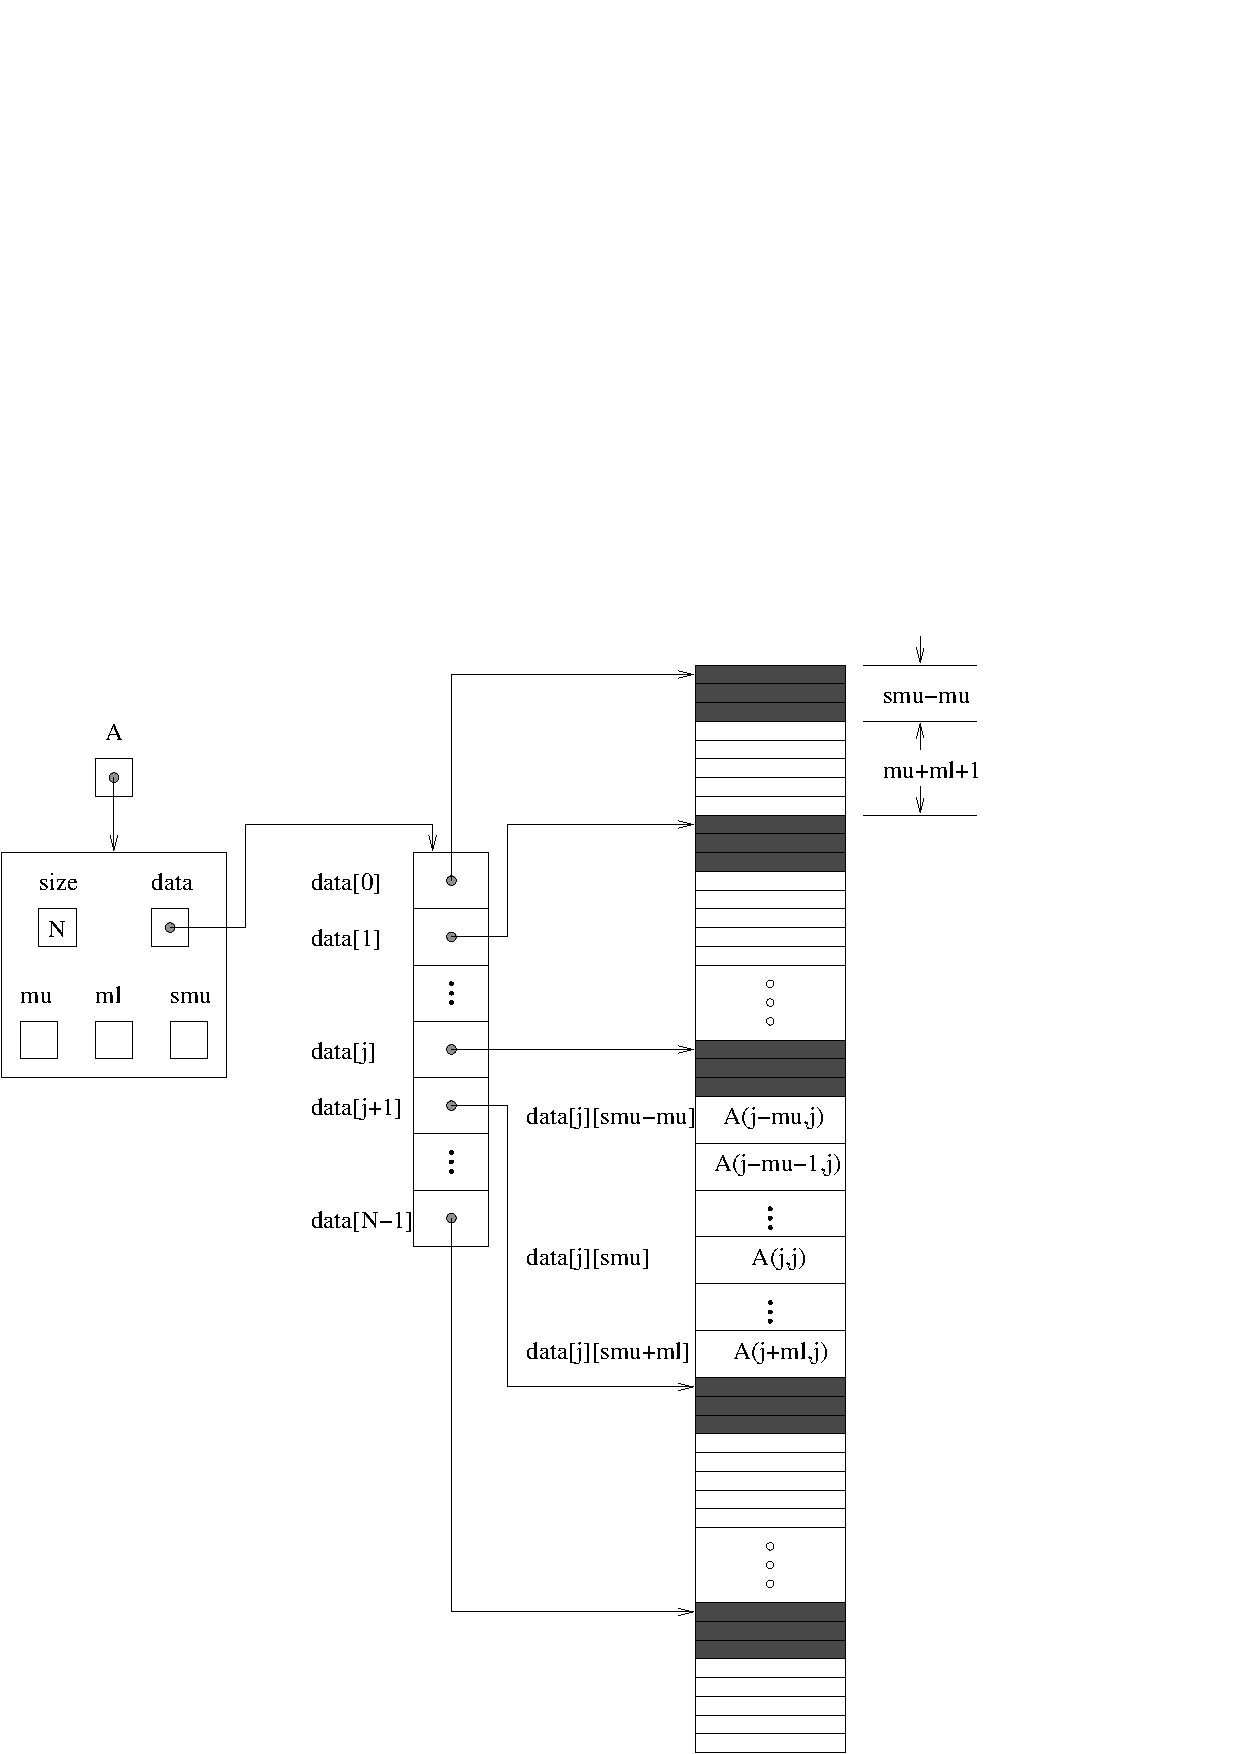
\includegraphics[width=4.5 in]{bandmat}}
\caption[Diagram of the storage for a {\sunmatband} object]
  {Diagram of the storage for the {\sunmatband} module. Here \id{A} is an
  $\id{N} \times \id{N}$ band matrix with upper and lower half-bandwidths \id{mu}
  and \id{ml}, respectively. The rows and columns of \id{A} are
  numbered from $0$ to $\id{N}-1$ and the ($i,j$)-th element of \id{A} is
  denoted \id{A(i,j)}. The greyed out areas of the underlying
  component storage are used by the associated {\sunlinsolband}
  linear solver.}\label{f:sunbandmat}
\end{figure}

\noindent The header file to include when using this module
is \id{sunmatrix/sunmatrix\_band.h}. The {\sunmatband} module
is accessible from all {\sundials} solvers \textit{without}
linking to the \newline
\id{libsundials\_sunmatrixband} module library.


% ====================================================================
\subsection{SUNMatrix\_Band accessor macros}
\label{ss:sunmat_band_macros}
% ====================================================================

The following macros are provided to access the
content of a {\sunmatband} matrix. The prefix \id{SM\_} in the names
denotes that these macros are for \emph{SUNMatrix} implementations,
and the suffix \id{\_B} denotes that these are specific to
the \emph{banded} version.
%%
\begin{itemize}

\item \ID{SM\_CONTENT\_B}

  This routine gives access to the contents of the
  banded \id{SUNMatrix}.

  The assignment \id{A\_cont} $=$ \id{SM\_CONTENT\_B(A)} sets
  \id{A\_cont} to be a pointer to the banded \id{SUNMatrix} content
  structure.

  Implementation:

  \verb|#define SM_CONTENT_B(A)     ( (SUNMatrixContent_Band)(A->content) )|

\item \ID{SM\_ROWS\_B}, \ID{SM\_COLUMNS\_B}, \ID{SM\_UBAND\_B}, \ID{SM\_LBAND\_B}, \ID{SM\_SUBAND\_B}, \ID{SM\_LDIM\_B}, and \ID{SM\_LDATA\_B}

  These macros give individual access to various lengths relevant to the
  content of a banded \id{SUNMatrix}.

  These may be used either to retrieve or to set these values.  For
  example, the assignment \id{A\_rows = SM\_ROWS\_B(A)} sets \id{A\_rows} to be
  the number of rows in the matrix \id{A}.  Similarly, the
  assignment \id{SM\_COLUMNS\_B(A) = A\_cols} sets the number of
  columns in \id{A} to equal \id{A\_cols}.

  Implementation:

  \verb|#define SM_ROWS_B(A)        ( SM_CONTENT_B(A)->M )|

  \verb|#define SM_COLUMNS_B(A)     ( SM_CONTENT_B(A)->N )|

  \verb|#define SM_UBAND_B(A)       ( SM_CONTENT_B(A)->mu )|

  \verb|#define SM_LBAND_B(A)       ( SM_CONTENT_B(A)->ml )|

  \verb|#define SM_SUBAND_B(A)      ( SM_CONTENT_B(A)->s_mu )|

  \verb|#define SM_LDIM_B(A)        ( SM_CONTENT_B(A)->ldim )|

  \verb|#define SM_LDATA_B(A)       ( SM_CONTENT_B(A)->ldata )|

\item \ID{SM\_DATA\_B} and \ID{SM\_COLS\_B}

  These macros give access to the \id{data} and \id{cols} pointers for
  the matrix entries.

  The assignment \id{A\_data = SM\_DATA\_B(A)} sets \id{A\_data} to be
  a pointer to the first component of the data array for the
  banded \id{SUNMatrix} \id{A}.  The assignment \id{SM\_DATA\_B(A) =
  A\_data} sets the data array of \id{A} to be \id{A\_data} by storing
  the pointer \id{A\_data}.

  Similarly, the assignment \id{A\_cols = SM\_COLS\_B(A)} sets \id{A\_cols} to be
  a pointer to the array of column pointers for the banded \id{SUNMatrix} \id{A}.
  The assignment \id{SM\_COLS\_B(A) = A\_cols} sets the column pointer
  array of \id{A} to be \id{A\_cols} by storing the pointer \id{A\_cols}.

  Implementation:

  \verb|#define SM_DATA_B(A)        ( SM_CONTENT_B(A)->data )|

  \verb|#define SM_COLS_B(A)        ( SM_CONTENT_B(A)->cols )|


\item \ID{SM\_COLUMN\_B}, \ID{SM\_COLUMN\_ELEMENT\_B}, and \ID{SM\_ELEMENT\_B}

  These macros give access to the individual columns and entries of
  the data array of a banded \id{SUNMatrix}.

  The assignments \id{SM\_ELEMENT\_B(A,i,j) = a\_ij} and \id{a\_ij =
  SM\_ELEMENT\_B(A,i,j)} reference the (\id{i},\id{j})-th element of the
  $\id{N} \times \id{N}$ band matrix \id{A}, where $0 \le \id{i}, \id{j} \le \id{N}-1$.
  The location (\id{i},\id{j}) should further satisfy
  \id{j}$-$\id{mu} $\le$ \id{i} $\le$ \id{j}$+$\id{ml}.

  The assignment \id{col\_j = SM\_COLUMN\_B(A,j)} sets \id{col\_j} to be
  a pointer to the diagonal element of the \id{j}-th column of the
  $\id{N} \times \id{N}$ band matrix \id{A}, $0 \le \id{j} \le \id{N}-1$.
  The type of the expression \id{SM\_COLUMN\_B(A,j)} is \id{realtype *}.
  The pointer returned by the call \id{SM\_COLUMN\_B(A,j)} can be treated as
  an array which is indexed from $-$\id{mu} to \id{ml}.

  The assignments \id{SM\_COLUMN\_ELEMENT\_B(col\_j,i,j) = a\_ij} and\\
  \id{a\_ij = SM\_COLUMN\_ELEMENT\_B(col\_j,i,j)} reference the
  (\id{i},\id{j})-th entry of the band matrix \id{A} when used in
  conjunction with \id{SM\_COLUMN\_B} to reference the \id{j}-th column
  through \id{col\_j}. The index (\id{i},\id{j}) should satisfy
  \id{j}$-$\id{mu} $\le$ \id{i} $\le$ \id{j}$+$\id{ml}.

  Implementation:

  \verb|#define SM_COLUMN_B(A,j)    ( ((SM_CONTENT_B(A)->cols)[j])+SM_SUBAND_B(A) )|

  \verb|#define SM_COLUMN_ELEMENT_B(col_j,i,j) (col_j[(i)-(j)])|

  \verb|#define SM_ELEMENT_B(A,i,j)|

  \hspace{1in} \verb|( (SM_CONTENT_B(A)->cols)[j][(i)-(j)+SM_SUBAND_B(A)] )|

\end{itemize}


% ====================================================================
\subsection{SUNMatrix\_Band functions}
\label{ss:sunmat_band_functions}
% ====================================================================

The {\sunmatband} module defines banded implementations of all matrix
operations listed in Table \ref{t:sunmatops}. Their names are obtained
from those in Table \ref{t:sunmatops} by appending the
suffix \id{\_Band} (e.g. \id{SUNMatCopy\_Band}).
All the standard matrix operations listed in \ref{t:sunmatops} with the suffix
\id{\_Band} appended are callable via the {\F} 2003 interface by prepending an
`F' (e.g. \id{FSUNMatCopy\_Band}).

The module {\sunmatband} provides the following additional user-callable routines:
%%--------------------------------------
\sunmodfunf{SUNBandMatrix}
{
  This constructor function creates and allocates memory for a banded \id{SUNMatrix}.
  Its arguments are the matrix size, \id{N}, and the upper and lower
  half-bandwidths of the matrix, \id{mu} and \id{ml}.  The stored
  upper bandwidth is set to \id{mu+ml} to accommodate subsequent
  factorization in the {\sunlinsolband} and {\sunlinsollapband} modules.
}
{
  SUNMatrix SUNBandMatrix(sunindextype N, sunindextype mu,
  sunindextype ml)
}
%%--------------------------------------
\sunmodfun{SUNBandMatrixStorage}
{
  This constructor function creates and allocates memory for a banded \id{SUNMatrix}.
  Its arguments are the matrix size, \id{N}, the upper and lower
  half-bandwidths of the matrix, \id{mu} and \id{ml}, and the stored
  upper bandwidth, \id{smu}.  When creating a band \id{SUNMatrix},
  this value should be
  \begin{itemize}
  \item at least min(\id{N}-1,\id{mu}+\id{ml}) if the matrix will be
    used by the {\sunlinsolband} module;
  \item exactly equal to \id{mu}+\id{ml} if the matrix will be used by
    the {\sunlinsollapband} module;
  \item at least \id{mu} if used in some other manner.
  \end{itemize}
  \emph{Note: it is strongly recommended that users call the default
    constructor, \id{SUNBandMatrix}, in all standard use cases.  This
    advanced constructor is used internally within {\sundials}
    solvers, and is provided to users who require banded matrices for
    non-default purposes.}
}
{
  SUNMatrix SUNBandMatrixStorage(sunindextype N, sunindextype mu,
  sunindextype ml, sunindextype smu)
}
%%--------------------------------------
\sunmodfun{SUNBandMatrix\_Print}
{
  This function prints the content of a banded \id{SUNMatrix} to the
  output stream specified by \id{outfile}.  Note: \id{stdout}
  or \id{stderr} may be used as arguments for \id{outfile} to print
  directly to standard output or standard error, respectively.
}
{
  void SUNBandMatrix\_Print(SUNMatrix A, FILE* outfile)
}
%%--------------------------------------
\sunmodfunf{SUNBandMatrix\_Rows}
{
  This function returns the number of rows in the banded \id{SUNMatrix}.
}
{
  sunindextype SUNBandMatrix\_Rows(SUNMatrix A)
}
%%--------------------------------------
\sunmodfunf{SUNBandMatrix\_Columns}
{
  This function returns the number of columns in the banded \id{SUNMatrix}.
}
{
  sunindextype SUNBandMatrix\_Columns(SUNMatrix A)
}
%%--------------------------------------
\sunmodfunf{SUNBandMatrix\_LowerBandwidth}
{
  This function returns the lower half-bandwidth of the banded \id{SUNMatrix}.
}
{
  sunindextype SUNBandMatrix\_LowerBandwidth(SUNMatrix A)
}
%%--------------------------------------
\sunmodfunf{SUNBandMatrix\_UpperBandwidth}
{
  This function returns the upper half-bandwidth of the banded \id{SUNMatrix}.
}
{
  sunindextype SUNBandMatrix\_UpperBandwidth(SUNMatrix A)
}
%%--------------------------------------
\sunmodfunf{SUNBandMatrix\_StoredUpperBandwidth}
{
  This function returns the stored upper half-bandwidth of the banded \id{SUNMatrix}.
}
{
  sunindextype SUNBandMatrix\_StoredUpperBandwidth(SUNMatrix A)
}
%%--------------------------------------
\sunmodfunf{SUNBandMatrix\_LDim}
{
  This function returns the length of the leading dimension of the banded \id{SUNMatrix}.
}
{
  sunindextype SUNBandMatrix\_LDim(SUNMatrix A)
}
%%--------------------------------------
\sunmodfunf{SUNBandMatrix\_Data}
{
  This function returns a pointer to the data array for the banded \id{SUNMatrix}.
}
{
  realtype* SUNBandMatrix\_Data(SUNMatrix A)
}
%%--------------------------------------
\sunmodfun{SUNBandMatrix\_Cols}
{
  This function returns a pointer to the cols array for the banded \id{SUNMatrix}.
}
{
  realtype** SUNBandMatrix\_Cols(SUNMatrix A)
}
%%--------------------------------------
\sunmodfunf{SUNBandMatrix\_Column}
{
  This function returns a pointer to the diagonal entry of the j-th
  column of the banded \id{SUNMatrix}.  The resulting pointer should
  be indexed over the range $-$\id{mu} to \id{ml}.
}
{
  realtype* SUNBandMatrix\_Column(SUNMatrix A, sunindextype j)
}
%%
%%------------------------------------
%%
\paragraph{\bf Notes}

\begin{itemize}

\item
  When looping over the components of a banded \id{SUNMatrix} \id{A},
  the most efficient approaches are to:
  \begin{itemize}
    \item First obtain the component array via \id{A\_data = SM\_DATA\_B(A)} or\\
    \id{A\_data = SUNBandMatrix\_Data(A)} and then
    access \id{A\_data[i]} within the loop.

    \item First obtain the array of column pointers via \id{A\_cols = SM\_COLS\_B(A)} or\\
    \id{A\_cols = SUNBandMatrix\_Cols(A)}, and then
    access \id{A\_cols[j][i]} within the loop.

    \item Within a loop over the columns, access the column pointer via\\
    \id{A\_colj = SUNBandMatrix\_Column(A,j)} and then to access the
    entries within that column using \id{SM\_COLUMN\_ELEMENT\_B(A\_colj,i,j)}.
  \end{itemize}
  All three of these are more efficient than
  using \id{SM\_ELEMENT\_B(A,i,j)} within a double loop.

\item
  {\warn} Within the \id{SUNMatMatvec\_Band} routine, internal
  consistency checks are performed to ensure that the matrix is called
  with consistent {\nvector} implementations.  These are currently
  limited to: {\nvecs}, {\nvecopenmp}, and {\nvecpthreads}.  As additional
  compatible vector implementations are added to {\sundials}, these
  will be included within this compatibility check.

\end{itemize}


% ====================================================================
\subsection{SUNMatrix\_Band Fortran interfaces}
\label{ss:sunmat_band_fortran}
% ====================================================================

The {\sunmatband} module provides a {\F} 2003 module as well as {\F} 77
style interface functions for use from {\F} applications.

\subsubsection*{FORTRAN 2003 interface module}
The \ID{fsunmatrix\_band\_mod} {\F} module defines interfaces to most
{\sunmatband} {\CC} functions using the intrinsic \id{iso\_c\_binding}
module which provides a standardized mechanism for interoperating with {\CC}. As
noted in the {\CC} function descriptions above, the interface functions are
named after the corresponding {\CC} function, but with a leading `F'. For
example, the function \id{SUNBandMatrix} is interfaced as
\id{FSUNBandMatrix}.

The {\F} 2003 {\sunmatband} interface module can be accessed with the \id{use}
statement, i.e. \id{use fsunmatrix\_band\_mod}, and linking to the library
\id{libsundials\_fsunmatrixband\_mod}.{\em lib} in addition to the {\CC} library.
For details on where the library and module file
\id{fsunmatrix\_band\_mod.mod} are installed see Appendix \ref{c:install}.
We note that the module is accessible from the {\F} 2003 {\sundials} integrators
\textit{without} separately linking to the
\id{libsundials\_fsunmatrixband\_mod} library.

\subsubsection*{FORTRAN 77 interface functions}
For solvers that include a {\F} interface module, the {\sunmatband}
module also includes the {\F}-callable
function \id{FSUNBandMatInit(code, N, mu, ml, ier)} to initialize
this {\sunmatband} module for a given {\sundials} solver.
Here \id{code} is an integer input solver id (1 for {\cvode}, 2 for {\ida}, 3
for {\kinsol}, 4 for {\arkode}); \id{N}, \id{mu}, and \id{ml}
are the corresponding band matrix construction arguments (declared
to match C type \id{long int}); and \id{ier} is an error return flag
equal to 0 for success and -1 for failure. Both \id{code} and \id{ier}
are declared to match C type \id{int}. Additionally, when using
{\arkode} with a non-identity mass matrix, the {\F}-callable
function \id{FSUNBandMassMatInit(N, mu, ml, ier)} initializes
this {\sunmatband} module for storing the mass matrix.

%% This is a shared SUNDIALS TEX file with a description of the
%% sparse sunmatrix implementation
%%
\section{The SUNMatrix\_Sparse implementation}\label{ss:sunmat_sparse}

The sparse implementation of the {\sunmatrix} module provided with
{\sundials}, {\sunmatsparse}, is designed to work with either
\emph{compressed-sparse-column} (CSC) or \emph{compressed-sparse-row}
(CSR) sparse matrix formats.  To this end, it defines the {\em
content} field of \id{SUNMatrix} to be the following structure:
%%
\begin{verbatim} 
struct _SUNMatrixContent_Sparse {
  sunindextype M;
  sunindextype N;
  sunindextype NNZ;
  sunindextype NP;
  realtype *data;
  int sparsetype;
  sunindextype *indexvals;
  sunindextype *indexptrs;
  /* CSC indices */
  sunindextype **rowvals;
  sunindextype **colptrs;
  /* CSR indices */
  sunindextype **colvals;
  sunindextype **rowptrs;
};
\end{verbatim}
%%
A diagram of the underlying data representation for a
CSC matrix is shown in Figure \ref{f:sparsemat} (the CSR format is
similar).  A more complete description of the parts of
this \emph{content} field is given below: 
\begin{args}[sparsetype]
  \item[M]  - number of rows
  \item[N]  - number of columns
  \item[NNZ]  - maximum number of nonzero entries in the matrix
    (allocated length of \id{data} and \id{indexvals} arrays)
  \item[NP]  - number of index pointers (e.g. number of column pointers for 
    CSC matrix). For CSC matrices $\id{NP}=\id{N}$, and for CSR
    matrices $\id{NP}=\id{M}$. This value is set automatically based
    the input for \verb|sparsetype|.
  \item[data]  - pointer to a contiguous block of \id{realtype}
    variables (of length \id{NNZ}), containing the values of the
    nonzero entries in the matrix
  \item[sparsetype]  - type of the sparse matrix (\id{CSC\_MAT} or \id{CSR\_MAT})
  \item[indexvals] - pointer to a contiguous block of \id{int} variables
    (of length \id{NNZ}), containing the row indices (if CSC) or column
   indices (if CSR) of each nonzero matrix entry held in \id{data}
  \item[indexptrs]  - pointer to a contiguous block of \id{int}
    variables (of length \id{NP+1}). For CSC matrices each 
    entry provides the index of the first column entry into the 
    \id{data} and \id{indexvals} arrays, e.g. if \id{indexptr[3]=7}, then 
    the first nonzero entry in the fourth column of the matrix is 
    located in \id{data[7]}, and is located in row \id{indexvals[7]} of the 
    matrix.  The last entry contains the total number of nonzero values in 
    the matrix and hence points one past the end of the active data in the 
    \id{data} and \id{indexvals} arrays. For CSR matrices, each entry provides 
    the index of the first row entry into the \id{data} and \id{indexvals} 
    arrays.
\end{args}
\noindent The following pointers are added to the \id{SlsMat} type for
  user convenience, to provide a more intuitive interface to the CSC
  and CSR sparse matrix data structures. They are set automatically
  when creating a sparse {\sunmatrix}, based on the sparse matrix storage
  type.  
\begin{args}[colptrs]
  \item[rowvals] - pointer to \verb|indexvals| when \id{sparsetype} is \id{CSC\_MAT},
    otherwise set to \verb|NULL|.
  \item[colptrs] - pointer to \verb|indexptrs| when \id{sparsetype} is \id{CSC\_MAT},
    otherwise set to \verb|NULL|.
  \item[colvals] - pointer to \verb|indexvals| when \id{sparsetype} is \id{CSR\_MAT},
    otherwise set to \verb|NULL|.
  \item[rowptrs] - pointer to \verb|indexptrs| when \id{sparsetype} is \id{CSR\_MAT},
    otherwise set to \verb|NULL|.
\end{args}
For example, the $5\times 4$ CSC matrix
\[
  \left[\begin{array}{cccc} 
     0 & 3 & 1 & 0\\
     3 & 0 & 0 & 2\\
     0 & 7 & 0 & 0\\
     1 & 0 & 0 & 9\\
     0 & 0 & 0 & 5
  \end{array}\right]
\]
could be stored in this structure as either
\begin{verbatim}
  M = 5;
  N = 4;
  NNZ = 8;
  NP = N;
  data = {3.0, 1.0, 3.0, 7.0, 1.0, 2.0, 9.0, 5.0};
  sparsetype = CSC_MAT;
  indexvals = {1, 3, 0, 2, 0, 1, 3, 4};
  indexptrs = {0, 2, 4, 5, 8};
\end{verbatim}
or 
\begin{verbatim}
  M = 5;
  N = 4;
  NNZ = 10;
  NP = N;
  data = {3.0, 1.0, 3.0, 7.0, 1.0, 2.0, 9.0, 5.0, *, *};
  sparsetype = CSC_MAT;
  indexvals = {1, 3, 0, 2, 0, 1, 3, 4, *, *};
  indexptrs = {0, 2, 4, 5, 8};
\end{verbatim}
where the first has no unused space, and the second has additional
storage (the entries marked with \texttt{*} may contain any values).
Note in both cases that the final value in \id{indexptrs} is $8$,
indicating the total number of nonzero entries in the matrix.

Similarly, in CSR format, the same matrix could be stored as
\begin{verbatim}
  M = 5;
  N = 4;
  NNZ = 8;
  NP = M;
  data = {3.0, 1.0, 3.0, 2.0, 7.0, 1.0, 9.0, 5.0};
  sparsetype = CSR_MAT;
  indexvals = {1, 2, 0, 3, 1, 0, 3, 3};
  indexptrs = {0, 2, 4, 5, 7, 8};
\end{verbatim}

%%
%%--------------------------------------------
%%
\begin{figure}
\centerline{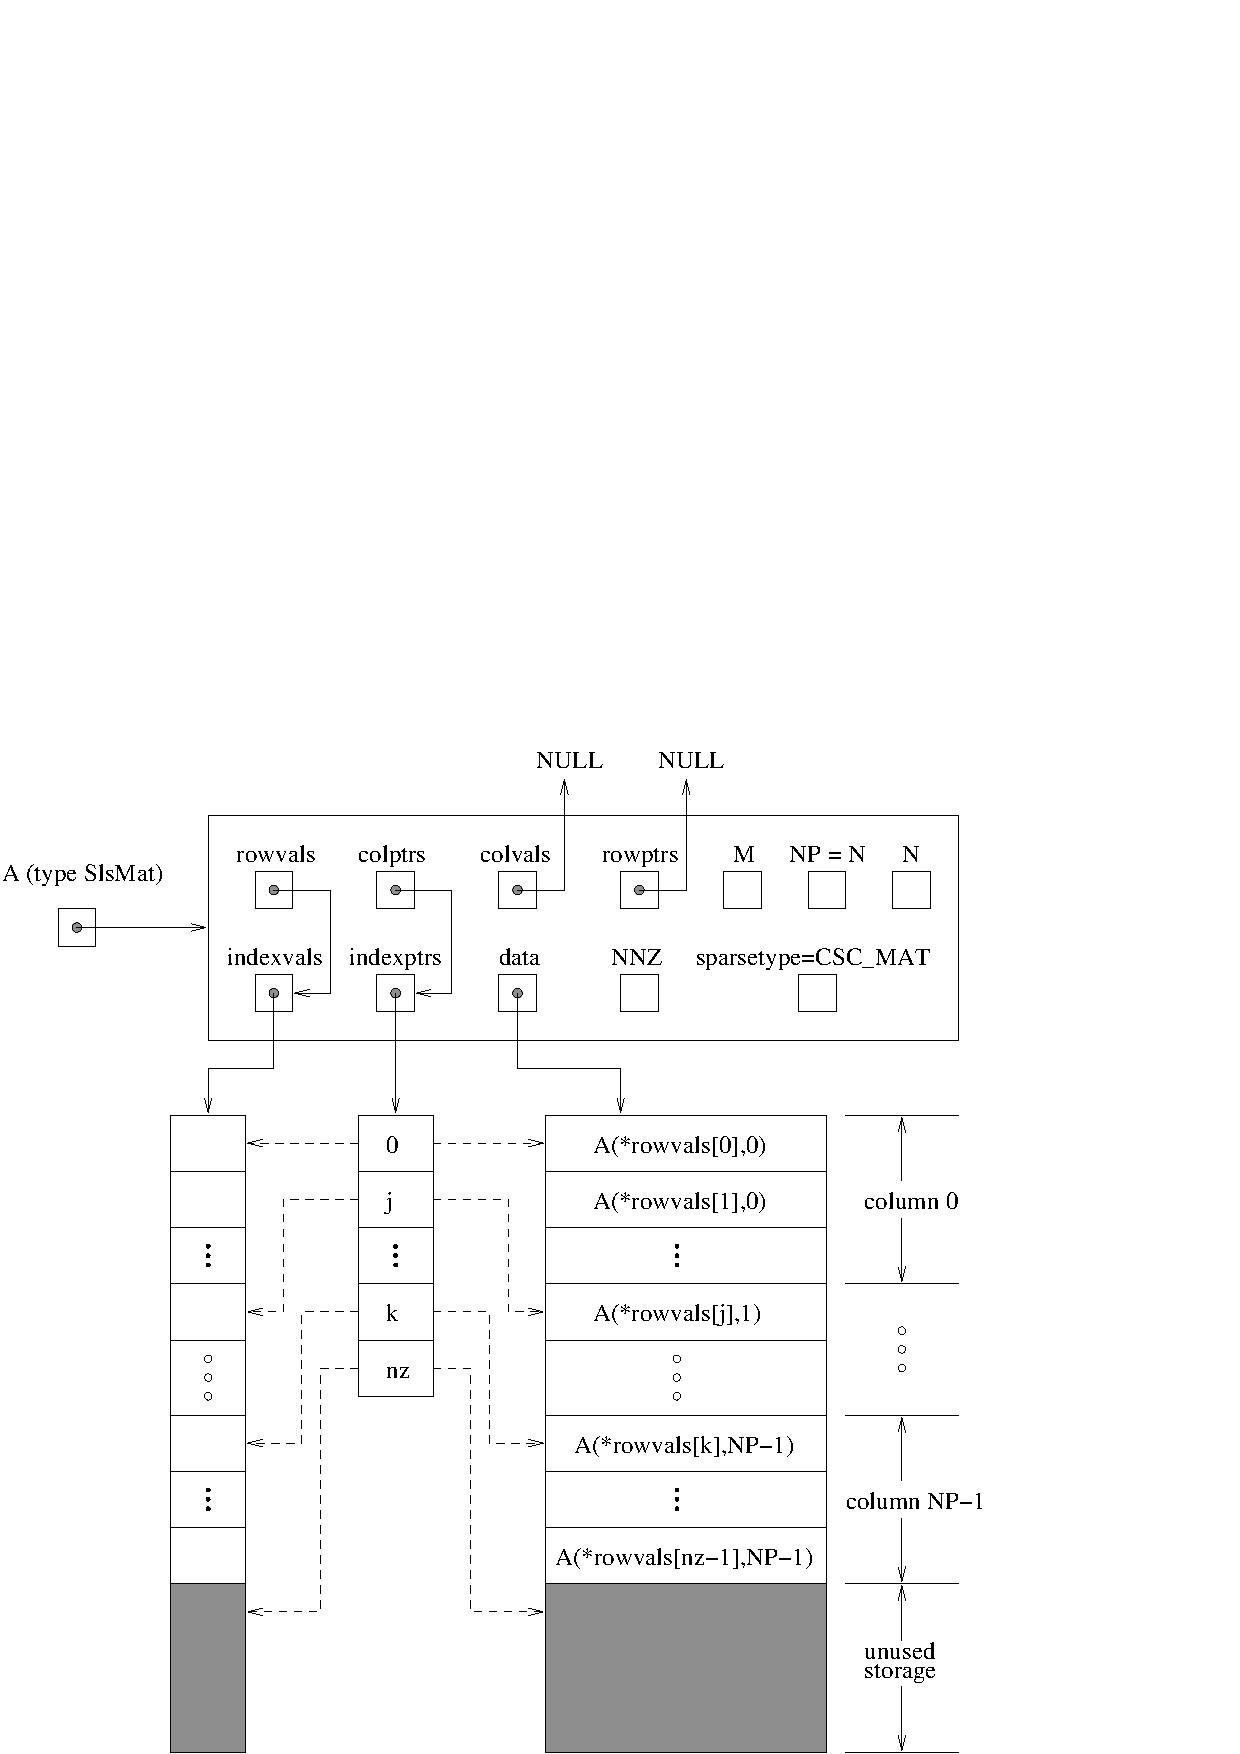
\includegraphics[width=4.5 in]{cscmat}}
\caption[Diagram of the storage for a compressed-sparse-column matrix] 
  {Diagram of the storage for a compressed-sparse-column
  matrix. Here \id{A} is an $\id{M} \times \id{N}$ sparse matrix with storage
  for up to \id{NNZ} nonzero entries (the allocated length of
  both \id{data} and \id{indexvals}).  The entries in \id{indexvals}
  may assume values from $0$ to $\id{M}-1$, corresponding to the row index
  (zero-based) of each nonzero value.  The entries in \id{data} contain
  the values of the nonzero entries, with the row $i$, column $j$
  entry of \id{A} (again, zero-based) denoted as \id{A(i,j)}.
  The \id{indexptrs} array contains $\id{N}+1$ entries; the first $\id{N}$
  denote the starting index of each column within the \id{indexvals}
  and \id{data} arrays, while the final entry points one past the
  final nonzero entry.  Here, although \id{NNZ} values are allocated,
  only \id{nz} are actually filled in; the greyed-out portions
  of \id{data} and \id{indexvals} indicate extra allocated
  space.}\label{f:sparsemat} 
\end{figure}

\noindent The header file to include when using this module 
is \id{sunmatrix/sunmatrix\_sparse.h}. The {\sunmatsparse} module
is accessible from all {\sundials} solvers \textit{without}
linking to the \\
\id{libsundials\_sunmatrixsparse} module library.


% ====================================================================
\subsection{SUNMatrix\_Sparse accessor macros}
\label{ss:sunmat_sparse_macros}
% ====================================================================

The following macros are provided to access the
content of a {\sunmatsparse} matrix. The prefix \id{SM\_} in the names
denotes that these macros are for \emph{SUNMatrix} implementations,
and the suffix \id{\_S} denotes that these are specific to
the \emph{sparse} version.
%%
\begin{itemize}

\item \ID{SM\_CONTENT\_S}
    
  This routine gives access to the contents of the
  sparse \id{SUNMatrix}.
  
  The assignment \id{A\_cont} $=$ \id{SM\_CONTENT\_S(A)} sets           
  \id{A\_cont} to be a pointer to the sparse \id{SUNMatrix} content  
  structure.                                             
                                                            
  Implementation: 
  
  \verb|#define SM_CONTENT_S(A)     ( (SUNMatrixContent_Sparse)(A->content) )|
  
\item \ID{SM\_ROWS\_S}, \ID{SM\_COLUMNS\_S}, \ID{SM\_NNZ\_S}, \ID{SM\_NP\_S}, and \ID{SM\_SPARSETYPE\_S}

  These macros give individual access to various lengths relevant to the
  content of a sparse \id{SUNMatrix}.
                                                               
  These may be used either to retrieve or to set these values.  For
  example, the assignment \id{A\_rows = SM\_ROWS\_S(A)} sets \id{A\_rows} to be
  the number of rows in the matrix \id{A}.  Similarly, the
  assignment \id{SM\_COLUMNS\_S(A) = A\_cols} sets the number of
  columns in \id{A} to equal \id{A\_cols}.
  
  Implementation: 
  
  \verb|#define SM_ROWS_S(A)        ( SM_CONTENT_S(A)->M )|

  \verb|#define SM_COLUMNS_S(A)     ( SM_CONTENT_S(A)->N )|

  \verb|#define SM_NNZ_S(A)         ( SM_CONTENT_S(A)->NNZ )|

  \verb|#define SM_NP_S(A)          ( SM_CONTENT_S(A)->NP )|

  \verb|#define SM_SPARSETYPE_S(A)  ( SM_CONTENT_S(A)->sparsetype )|


\item \ID{SM\_DATA\_S}, \ID{SM\_INDEXVALS\_S}, and \ID{SM\_INDEXPTRS\_S}
                                                            
  These macros give access to the \id{data} and index arrays for
  the matrix entries.

  The assignment \id{A\_data = SM\_DATA\_S(A)} sets \id{A\_data} to be     
  a pointer to the first component of the data array for the
  sparse \id{SUNMatrix} \id{A}.  The assignment \id{SM\_DATA\_S(A) =
  A\_data} sets the data array of \id{A} to be \id{A\_data} by storing
  the pointer \id{A\_data}. 
  
  Similarly, the assignment \id{A\_indexvals = SM\_INDEXVALS\_S(A)}
  sets \id{A\_indexvals} to be a pointer to the array of index values
  (i.e.~row indices for a CSC matrix, or column indices for a CSR
  matrix) for the sparse \id{SUNMatrix} \id{A}.  The
  assignment \id{A\_indexptrs = SM\_INDEXPTRS\_S(A)}
  sets \id{A\_indexptrs} to be a pointer to the array of index
  pointers (i.e.~the starting indices in the data/indexvals arrays for
  each row or column in CSR or CSC formats, respectively).
  
  Implementation:

  \verb|#define SM_DATA_S(A)        ( SM_CONTENT_S(A)->data )|

  \verb|#define SM_INDEXVALS_S(A)   ( SM_CONTENT_S(A)->indexvals )|

  \verb|#define SM_INDEXPTRS_S(A)   ( SM_CONTENT_S(A)->indexptrs )|

\end{itemize}


% ====================================================================
\subsection{SUNMatrix\_Sparse functions}
\label{ss:sunmat_sparse_functions}
% ====================================================================

The {\sunmatsparse} module defines sparse implementations of all matrix
operations listed in Section \ref{ss:sunmatrix_functions}. Their names are obtained
from those in Section \ref{ss:sunmatrix_functions} by appending the
suffix \id{\_Sparse} (e.g. \id{SUNMatCopy\_Sparse}). 
All the standard matrix operations listed in Section \ref{ss:sunmatrix_functions} with the suffix
\id{\_Sparse} appended are callable via the {\F} 2003 interface by prepending an
`F' (e.g. \id{FSUNMatCopy\_Sparse}).

The module {\sunmatsparse} provides the following additional
user-callable routines: 
%%--------------------------------------
\sunmodfunf{SUNSparseMatrix}
{
  This function creates and allocates memory for a sparse \id{SUNMatrix}.
  Its arguments are the number of rows and columns of the
  matrix, \id{M} and \id{N}, the maximum number of nonzeros to be
  stored in the matrix, \id{NNZ}, and a flag \id{sparsetype}
  indicating whether to use CSR or CSC format (valid arguments
  are \id{CSR\_MAT} or \id{CSC\_MAT}). 
}
{
  SUNMatrix SUNSparseMatrix(sunindextype M, sunindextype N,
  \newlinefill{SUNMatrix SUNSparseMatrix}
  sunindextype NNZ, int sparsetype)
}
%%--------------------------------------
\sunmodfunf{SUNSparseFromDenseMatrix}
{
  This function creates a new sparse matrix from an existing dense
  matrix by copying all values with magnitude larger than \id{droptol}
  into the sparse matrix structure.

  Requirements:
  \begin{itemize}
  \item \id{A} must have type \id{SUNMATRIX\_DENSE};
  \item \id{droptol} must be non-negative;
  \item \id{sparsetype} must be either \id{CSC\_MAT} or \id{CSR\_MAT}.
  \end{itemize}
  The function returns NULL if any requirements are violated, or if
  the matrix storage request cannot be satisfied. 
}
{
  SUNMatrix SUNSparseFromDenseMatrix(SUNMatrix A, realtype droptol,
  \newlinefill{SUNMatrix SUNSparseFromDenseMatrix}
  int sparsetype);
}
%%--------------------------------------
\sunmodfunf{SUNSparseFromBandMatrix}
{
  This function creates a new sparse matrix from an existing band
  matrix by copying all values with magnitude larger than \id{droptol}
  into the sparse matrix structure.

  Requirements:
  \begin{itemize}
  \item \id{A} must have type \id{SUNMATRIX\_BAND};
  \item \id{droptol} must be non-negative;
  \item \id{sparsetype} must be either \id{CSC\_MAT} or \id{CSR\_MAT}.
  \end{itemize}
  The function returns NULL if any requirements are violated, or if
  the matrix storage request cannot be satisfied. 
}
{
  SUNMatrix SUNSparseFromBandMatrix(SUNMatrix A, realtype droptol,
  \newlinefill{SUNMatrix SUNSparseFromBandMatrix}
  int sparsetype);
}
%%--------------------------------------
\sunmodfunf{SUNSparseMatrix\_Realloc}
{
  This function reallocates internal storage arrays in a sparse matrix
  so that the resulting sparse matrix has no wasted space (i.e.~the
  space allocated for nonzero entries equals the actual number of
  nonzeros, \id{indexptrs[NP]}). Returns 0 on success and 
  1 on failure (e.g.~if the input matrix is not sparse).
}
{
  int SUNSparseMatrix\_Realloc(SUNMatrix A)
}
%%--------------------------------------
\sunmodfunf{SUNSparseMatrix\_Reallocate}
{
  This function reallocates internal storage arrays in a sparse matrix
  so that the resulting sparse matrix has storage for a specified
  number of nonzeros. Returns 0 on success and 
  1 on failure (e.g.~if the input matrix is not sparse or if NNZ is
  negative). 
}
{
  int SUNSparseMatrix\_Reallocate(SUNMatrix A, sunindextype NNZ)
}
%%--------------------------------------
\sunmodfun{SUNSparseMatrix\_Print}
{
  This function prints the content of a sparse \id{SUNMatrix} to the
  output stream specified by \id{outfile}.  Note: \id{stdout}
  or \id{stderr} may be used as arguments for \id{outfile} to print
  directly to standard output or standard error, respectively.
}
{
  void SUNSparseMatrix\_Print(SUNMatrix A, FILE* outfile)
}
%%--------------------------------------
\sunmodfunf{SUNSparseMatrix\_Rows}
{
  This function returns the number of rows in the sparse \id{SUNMatrix}.
}
{
  sunindextype SUNSparseMatrix\_Rows(SUNMatrix A)
}
%%--------------------------------------
\sunmodfunf{SUNSparseMatrix\_Columns}
{
  This function returns the number of columns in the sparse \id{SUNMatrix}.
}
{
  sunindextype SUNSparseMatrix\_Columns(SUNMatrix A)
}
%%--------------------------------------
\sunmodfunf{SUNSparseMatrix\_NNZ}
{
  This function returns the number of entries allocated for nonzero
  storage for  the sparse matrix \id{SUNMatrix}.
}
{
  sunindextype SUNSparseMatrix\_NNZ(SUNMatrix A)
}
%%--------------------------------------
\sunmodfunf{SUNSparseMatrix\_NP}
{
  This function returns the number of columns/rows for the
  sparse \id{SUNMatrix}, depending on whether the matrix uses CSC/CSR
  format, respectively.  The \id{indexptrs} array has \id{NP+1} entries.
}
{
  sunindextype SUNSparseMatrix\_NP(SUNMatrix A)
}
%%--------------------------------------
\sunmodfunf{SUNSparseMatrix\_SparseType}
{
  This function returns the storage type (\id{CSR\_MAT}
  or \id{CSC\_MAT}) for the sparse \id{SUNMatrix}.
}
{
  int SUNSparseMatrix\_SparseType(SUNMatrix A)
}
%%--------------------------------------
\sunmodfunf{SUNSparseMatrix\_Data}
{
  This function returns a pointer to the data array for the
  sparse \id{SUNMatrix}. 
}
{
  realtype* SUNSparseMatrix\_Data(SUNMatrix A)
}
%%--------------------------------------
\sunmodfunf{SUNSparseMatrix\_IndexValues}
{
  This function returns a pointer to index value array for the sparse
  \id{SUNMatrix}: for CSR format this is the column index for each nonzero
  entry, for CSC format this is the row index for each nonzero entry.
}
{
  sunindextype* SUNSparseMatrix\_IndexValues(SUNMatrix A)
}
%%--------------------------------------
\sunmodfunf{SUNSparseMatrix\_IndexPointers}
{
  This function returns a pointer to the index pointer array for the
  sparse \id{SUNMatrix}: for CSR format this is the location of the first
  entry of each row in the \id{data} and \id{indexvalues} arrays, for
  CSC format this is the location of the first entry of each column.
}
{
  sunindextype* SUNSparseMatrix\_IndexPointers(SUNMatrix A)
}
%%
%%------------------------------------
%%
{\warn} Within the \id{SUNMatMatvec\_Sparse} routine, internal
consistency checks are performed to ensure that the matrix is called
with consistent {\nvector} implementations.  These are currently
limited to: {\nvecs}, {\nvecopenmp}, {\nvecpthreads}, and {\nveccuda}
when using managed memory.  As additional compatible vector implementations
are added to {\sundials}, these will be included within this compatibility check. 


% ====================================================================
\subsection{SUNMatrix\_Sparse Fortran interfaces}
\label{ss:sunmat_sparse_fortran}
% ====================================================================

The {\sunmatsparse} module provides a {\F} 2003 module as well as {\F} 77
style interface functions for use from {\F} applications.

\subsubsection*{FORTRAN 2003 interface module}
The \ID{fsunmatrix\_sparse\_mod} {\F} module defines interfaces to most
{\sunmatsparse} {\CC} functions using the intrinsic \id{iso\_c\_binding}
module which provides a standardized mechanism for interoperating with {\CC}. As
noted in the {\CC} function descriptions above, the interface functions are
named after the corresponding {\CC} function, but with a leading `F'. For
example, the function \id{SUNSparseMatrix} is interfaced as
\id{FSUNSparseMatrix}.

The {\F} 2003 {\sunmatsparse} interface module can be accessed with the \id{use}
statement, i.e. \id{use fsunmatrix\_sparse\_mod}, and linking to the library
\id{libsundials\_fsunmatrixsparse\_mod}.{\em lib} in addition to the {\CC} library.
For details on where the library and module file
\id{fsunmatrix\_sparse\_mod.mod} are installed see Appendix \ref{c:install}.
We note that the module is accessible from the {\F} 2003 {\sundials} integrators
\textit{without} separately linking to the
\id{libsundials\_fsunmatrixsparse\_mod} library.

\subsubsection*{FORTRAN 77 interface functions}
For solvers that include a Fortran interface module, the {\sunmatsparse}
module also includes the Fortran-callable
function \id{FSUNSparseMatInit(code, M, N, NNZ, sparsetype, ier)} to
initialize this {\sunmatsparse} module for a given {\sundials} solver.
Here \id{code} is an integer input for the solver id (1 for {\cvode},
2 for {\ida}, 3 for {\kinsol}, 4 for {\arkode}); \id{M}, \id{N}
and \id{NNZ} are the corresponding sparse matrix construction
arguments (declared to match C type \id{long
int}); \id{sparsetype} is an integer flag indicating the sparse
storage type (0 for CSC, 1 for CSR); and \id{ier} is an error return
flag equal to 0 for success and -1 for failure. Each of \id{code},
\id{sparsetype} and \id{ier} are declared so as to match C
type \id{int}. Additionally, when using {\arkode} with a non-identity
mass matrix, the Fortran-callable
function \id{FSUNSparseMassMatInit(M, N, NNZ, sparsetype, ier)} 
initializes this {\sunmatsparse} module for storing the mass matrix.

%% This is a shared SUNDIALS TEX file with a description of the
%% SuperLU_DIST SLUNRloc SUNMatrix implementation
%%
\section{The SUNMatrix\_SLUNRloc implementation}\label{ss:sunmat_slunrloc}

The {\sunmatslunrloc} implementation of the {\sunmatrix} module provided with
{\sundials} is an adapter for the \id{SuperMatrix} structure provided by the
{\superludist} sparse matrix factorization and solver library written by
X. Sherry Li \cite{SuperLUDIST_site,GDL:07,LD:03,SLUUG:99}.
It is designed to be used with the {\sunlinsolsludist} linear solver
discussed in Section~\ref{ss:sunlinsol_sludist}. To this end, it defines the
{\em content} field of \id{SUNMatrix} to be the following structure:
%%
\begin{verbatim}
struct _SUNMatrixContent_SLUNRloc {
  booleantype   own_data;
  gridinfo_t    *grid;
  sunindextype  *row_to_proc;
  pdgsmv_comm_t *gsmv_comm;
  SuperMatrix   *A_super;
  SuperMatrix   *ACS_super;
};
\end{verbatim}
%%

A more complete description of the this \emph{content} field is given below:

\begin{description}
  \item[own\_data] - a flag which indicates if the SUNMatrix is responsible for freeing
    \id{A\_super}
  \item[grid] - pointer to the {\superludist} structure that stores the 2D process grid
  \item[row\_to\_proc] - a mapping between the rows in the matrix and the process it
    resides on; will be \id{NULL} until the \id{SUNMatMatvecSetup} routine is called
  \item[gsmv\_comm] - pointer to the {\superludist} structure that stores the
    communication information needed for matrix-vector multiplication; will be
    \id{NULL} until the \id{SUNMatMatvecSetup} routine is called
  \item[A\_super] - pointer to the underlying {\superludist} \id{SuperMatrix} with
      \id{Stype = SLU\_NR\_loc, Dtype = SLU\_D, Mtype = SLU\_GE}; must have the
      full diagonal present to be used with \id{SUNMatScaleAddI} routine
  \item[ACS\_super] - a column-sorted version of the matrix needed to perform matrix-vector
    multiplication; will be \id{NULL} until the routine \id{SUNMatMatvecSetup}
    routine is called
\end{description}

\noindent The header file to include when using this module
is \id{sunmatrix/sunmatrix\_slunrloc.h}. The installed module
library to link to is \id{libsundials\_sunmatrixslunrloc.\textit{lib}}
where \id{\em.lib} is typically \id{.so} for shared libraries and
\id{.a} for static libraries.


% ====================================================================
\subsection{SUNMatrix\_SLUNRloc functions}
\label{ss:sunmat_slunrloc_functions}
% ====================================================================

The module {\sunmatslunrloc} provides the following user-callable routines:
%%--------------------------------------
%%
\ucfunction{SUNMatrix\_SLUNRloc}
{
  A = SUNMatrix\_SLUNRloc(Asuper, grid);
}
{
  The function \ID{SUNMatrix\_SLUNRloc} creates and allocates memory for a
  {\sunmatslunrloc} object.
}
{
  \begin{args}
  \item[Asuper] (\id{SuperMatrix*})
      a fully-allocated {\superludist} \id{SuperMatrix} that the SUNMatrix will
      wrap; must have \id{Stype = SLU\_NR\_loc, Dtype = SLU\_D, Mtype = SLU\_GE}
      to be compatible
  \item[grid] (\id{gridinfo\_t*}) the initialized {\superludist} 2D process grid structure
  \end{args}
}
{
  a \id{SUNMatrix} object if \id{Asuper} is compatible else \id{NULL}
}
{
}

\ucfunction{SUNMatrix\_SLUNRloc\_Print}
{
  SUNMatrix\_SLUNRloc\_Print(A, fp);
}
{
  The function \ID{SUNMatrix\_SLUNRloc\_Print} prints the underlying
  \id{SuperMatrix} content.
}
{
  \begin{args}
  \item[A] (\id{SUNMatrix}) the matrix to print
  \item[fp] (\id{FILE}) the file pointer used for printing
  \end{args}
}
{
  \id{void}
}
{
}

\ucfunction{SUNMatrix\_SLUNRloc\_SuperMatrix}
{
  Asuper = SUNMatrix\_SLUNRloc\_SuperMatrix(A);
}
{
  The function \ID{SUNMatrix\_SLUNRloc\_SuperMatrix} provides access
  to the underlying {\superludist} \id{SuperMatrix} of \id{A}.
}
{
  \begin{args}
  \item[A] (\id{SUNMatrix}) the matrix to access
  \end{args}
}
{
  \id{SuperMatrix*}
}
{
}

\ucfunction{SUNMatrix\_SLUNRloc\_ProcessGrid}
{
  grid = SUNMatrix\_SLUNRloc\_ProcessGrid(A);
}
{
  The function \ID{SUNMatrix\_SLUNRloc\_ProcessGrid} provides access
  to the {\superludist} \id{gridinfo\_t} structure associated with \id{A}.
}
{
  \begin{args}
  \item[A] (\id{SUNMatrix}) the matrix to access
  \end{args}
}
{
  \id{gridinfo\_t*}
}
{
}

\ucfunction{SUNMatrix\_SLUNRloc\_OwnData}
{
  does\_own\_data = SUNMatrix\_SLUNRloc\_OwnData(A);
}
{
  The function \ID{SUNMatrix\_SLUNRloc\_OwnData} returns true if the \id{SUNMatrix}
  object is responsible for freeing \id{A\_super}, otherwise it returns false.
}
{
  \begin{args}
  \item[A] (\id{SUNMatrix}) the matrix to access
  \end{args}
}
{
  \id{booleantype}
}
{
}

The {\sunmatslunrloc} module defines implementations of all generic \id{SUNMatrix} operations
listed in Table \ref{t:sunmatops}:

\begin{itemize}
  \item \id{SUNMatGetID\_SLUNRloc} - returns \id{SUNMATRIX\_SLUNRLOC}
  \item \id{SUNMatClone\_SLUNRloc}
  \item \id{SUNMatDestroy\_SLUNRloc}
  \item \id{SUNMatSpace\_SLUNRloc} - this only returns information for the storage within the
    matrix interface, i.e. storage for \id{row\_to\_proc}
  \item \id{SUNMatZero\_SLUNRloc}
  \item \id{SUNMatCopy\_SLUNRloc}
  \item \id{SUNMatScaleAdd\_SLUNRloc} - performs $A = cA + B$, but $A$ and $B$ must have the same sparsity pattern 
  \item \id{SUNMatScaleAddI\_SLUNRloc} - performs $A = cA + I$, but the diagonal of $A$ must be present
  \item \id{SUNMatMatvecSetup\_SLUNRloc} - initializes the {\superludist} parallel communication
    structures needed to perform a matrix-vector product; only needs to be called before the
    first call to \id{SUNMatMatvec} or if the matrix changed since the last setup
  \item \id{SUNMatMatvec\_SLUNRloc}
\end{itemize}

%%------------------------------------
%%
{\warn} The {\sunmatslunrloc} module requires that the complete diagonal, i.e. nonzeros and zeros,
is present in order to use the \id{SUNMatScaleAddI} operation.

% % ====================================================================
% \subsection{SUNMatrix\_SLUNRloc Fortran interfaces}
% \label{ss:sunmat_slunrloc_fortran}
% % ====================================================================

% The {\sunmatslunrloc} module provides a {\F} 2003 module as well as {\F} 77
% style interface functions for use from {\F} applications.

% \subsubsection*{FORTRAN 2003 interface module}
% The \ID{fsunmatrix\_slunrloc\_mod} {\F} module defines interfaces to most
% {\sunmatslunrloc} {\CC} functions using the intrinsic \id{iso\_c\_binding}
% module which provides a standardized mechanism for interoperating with {\CC}. As
% noted in the {\CC} function descriptions above, the interface functions are
% named after the corresponding {\CC} function, but with a leading `F'. For
% example, the function \id{SUNMatrix\_SLUNRloc} is interfaced as
% \id{FSUNMatrix\_SLUNRloc}.

% The {\F} 2003 {\sunmatslunrloc} interface module can be accessed with the \id{use}
% statement, i.e. \id{use fsunmatrix\_slunrloc\_mod}, and linking to the library
% \id{libsundials\_fsunmatrixslunrloc\_mod}.{\em lib} in addition to the {\CC} library.
% For details on where the library and module file \id{fsunmatrix\_slunrloc\_mod.mod}
% are installed see Appendix \ref{c:install}.



\clearemptydoublepage
%===============================================================
% Description of the SUNLinearSolver Concept
%===================================================================================
\chapter{Description of the SUNLinearSolver module}\label{s:sunlinsol}
%===================================================================================
\index{SUNLinearSolver@\texttt{SUNLinearSolver} module}
% This is a shared SUNDIALS TEX file with description of
% the generic sunlinsol abstraction
%
For problems that involve the solution of linear systems of equations,
the {\sundials} packages operate using generic linear solver modules
defined through the {\sunlinsol} API.  This allows {\sundials}
packages to utilize any valid {\sunlinsol} implementation that provides
a set of required functions.  These functions can be divided into
three categories.  The first are the core linear solver functions.  The
second group consists of ``set'' routines to supply the linear solver object
with functions provided by the {\sundials} package, or for modification
of solver parameters.  The last group consists of ``get'' routines for
retrieving artifacts (statistics, residual vectors, etc.) from the
linear solver.  All of these functions are defined in the header file
\Id{sundials/sundials\_linearsolver.h}.

The implementations provided with {\sundials} work in coordination
with the {\sundials} generic {\nvector} and {\sunmatrix} modules to
provide a set of compatible data structures and solvers for the
solution of linear systems using direct or matrix-free iterative
methods. Moreover, advanced users can provide a customized
\Id{SUNLineaerSolver} implementation to any {\sundials} package,
particularly in cases where they provide their own {\nvector} and/or
{\sunmatrix} modules.

Historically, the {\sundials} packages have been designed to specifically
leverage the use of either \emph{direct linear solvers} or matrix-free,
\emph{scaled, preconditioned, iterative linear solvers}.  However,
matrix-based iterative linear solvers are supported.

The iterative linear solvers packaged with {\sundials} leverage
scaling and preconditioning, as applicable, to balance error between
solution components and to accelerate convergence of the linear
solver.  To this end, instead of solving the  linear system $Ax = b$
directly, these apply the underlying iterative algorithm to the
transformed system
\begin{equation}
  \label{eq:transformed_linear_system}
  \tilde{A} \tilde{x} = \tilde{b}
\end{equation}
where
\begin{align}
  \notag
  \tilde{A} &= S_1 P_1^{-1} A P_2^{-1} S_2^{-1},\\
  \label{eq:transformed_linear_system_components}
  \tilde{b} &= S_1 P_1^{-1} b,\\
  \notag
  \tilde{x} &= S_2 P_2 x,
\end{align}
and where
\begin{itemize}
\item $P_1$ is the left preconditioner,
\item $P_2$ is the right preconditioner,
\item $S_1$ is a diagonal matrix of scale factors for $P_1^{-1} b$,
\item $S_2$ is a diagonal matrix of scale factors for $P_2 x$.
\end{itemize}
{\sundials} packages request that iterative linear solvers stop
based on the 2-norm of the scaled preconditioned residual meeting a
prescribed tolerance
\[
  \left\| \tilde{b} - \tilde{A} \tilde{x} \right\|_2  <  \text{tol}.
\]

When provided an iterative {\sunlinsol} implementation that does not
support the scaling matrices $S_1$ and $S_2$, {\sundials}'
packages will adjust the value of $\text{tol}$ accordingly.  In
this case, they instead request that iterative linear solvers stop
based on the criteria
\[
   \left\| P_1^{-1} b - P_1^{-1} A x \right\|_2  <  \text{tol}.
\]
We note that the corresponding adjustments to $\text{tol}$ in
this case are non-optimal, in that they cannot balance error between
specific entries of the solution $x$, only the aggregate error
in the overall solution vector.

We further note that not all of the {\sundials}-provided iterative
linear solvers support the full range of the above options (e.g.,
separate left/right preconditioning), and that some of the {\sundials}
packages only utilize a subset of these options.  Further details on
these exceptions are described in the documentation for each
{\sunlinsol} implementation, or for each {\sundials} package.

%---------------------------------------------------------------------------
\subsection{\id{SUNLinearSolver} core functions}\label{ss:sunlinsol_CoreFn}

The core linear solver functions consist of four required routines to get
the linear solver type \\ \noindent (\Id{SUNLinSolGetType}), initialize
the linear solver object once all solver-specific options have been
set (\Id{SUNLinSolInitialize}), set up the linear solver object
to utilize an updated matrix $A$ \\ \noindent (\Id{SUNLinSolSetup}),
and solve the linear system $Ax=b$ (\Id{SUNLinSolSolve}).
The remaining routine for destruction of the linear solver object
(\Id{SUNLinSolFree}) is optional.

% --------------------------------------------------------------------
\ucfunction{SUNLinSolGetType}
{
  type = SUNLinSolGetType(LS);
}
{
  The \textit{required} function \Id{SUNLinSolGetType} returns the
  type identifier for the linear solver \id{LS}. It is used to
  determine the solver type (direct or iterative) from
  the abstract \id{SUNLinearSolver} interface.  This is used to assess
  compatibility with {\sundials}-provided linear solver interfaces.
}
{
  \begin{args}[LS]
  \item[LS] (\id{SUNLinearSolver})
    a {\sunlinsol} object.
  \end{args}
}
{
  The return value \id{type} (of type \id{int}) will be one of the
  following:
  \begin{args}[SUNLINEARSOLVER\_ITERATIVE]
  \item[\Id{SUNNONLINEARSOLVER\_DIRECT}]
    \id{0}, the {\sunlinsol} module uses direct methods to solve the
    linear system.
  \item[\Id{SUNNONLINEARSOLVER\_ITERATIVE}]
    \id{1}, the {\sunlinsol} module iteratively solves the linear
    system, stopping when the linear residual is within a prescribed
    tolerance.
  \end{args}
}
{
}
% --------------------------------------------------------------------
\ucfunction{SUNLinSolInitialize}
{
  retval = SUNLinSolInitialize(LS);
}
{
  The \textit{required} function \Id{SUNLinSolInitialize} performs
  linear solver initialization (assumes that all solver-specific
  options have been set).
}
{
  \begin{args}[LS]
  \item[LS] (\id{SUNLinearSolver})
    a {\sunlinsol} object.
  \end{args}
}
{
  This should return zero for a
  successful call, and a negative value for a failure, ideally
  returning one of the generic error codes listed in Table
  \ref{t:sunlinsolerr}.
}
{
}
% --------------------------------------------------------------------
\ucfunction{SUNLinSolSetup}
{
  retval = SUNLinSolSetup(LS, A);
}
{
  The \textit{required} function \Id{SUNLinSolSetup} performs
  any linear solver setup needed, based on an updated system
  {\sunmatrix} \id{A}.  This may be called frequently (e.g. with a full
  Newton method) or infrequently (for a modified Newton method), based
  on the type of integrator and/or nonlinear solver requesting the
  solves.
}
{
  \begin{args}[LS]
  \item[LS] (\id{SUNLinearSolver})
    a {\sunlinsol} object.
  \item[A] (\id{SUNMatrix})
    a {\sunmatrix} object.
  \end{args}
}
{
  This should return zero for a successful call, a positive
  value for a recoverable failure and a negative value for an
  unrecoverable failure, ideally returning one of the generic error
  codes listed in Table \ref{t:sunlinsolerr}.
}
{
}
% --------------------------------------------------------------------
\ucfunction{SUNLinSolSolve}
{
  retval = SUNLinSolSolve(LS, A, x, b, tol);
}
{
  The \textit{required} function \Id{SUNLinSolSolve} solves a linear system $Ax = b$.
}
{
  \begin{args}[LS]
  \item[LS] (\id{SUNLinearSolver})
    a {\sunlinsol} object.
  \item[A] (\id{SUNMatrix})
    a {\sunmatrix} object.
  \item[x] (\id{N\_Vector})
    a {\nvector} object.
  \item[b] (\id{N\_Vector})
    a {\nvector} object.
  \item[tol] (\id{realtype})
    the desired linear solver tolerance.
  \end{args}
}
{
  This should return zero for
  a successful call, a positive value for a recoverable failure and a
  negative value for an unrecoverable failure, ideally returning one
  of the generic error codes listed in Table \ref{t:sunlinsolerr}.
}
{
  {\bf Direct solvers:} can ignore the  *tol* argument.

  {\bf Matrix-free solvers:} can ignore the {\sunmatrix} input \id{A}
  since a \id{NULL} argument will be passed (these should instead rely
  on the matrix-vector product function supplied through the routine
  \id{SUNLinSolSetATimes}.

  {\bf Iterative solvers:} These should attempt to solve to the
  specified tolerance \id{tol} in a weighted 2-norm.  If the solver
  does not support scaling then it should just use a 2-norm.
}
% --------------------------------------------------------------------
\ucfunction{SUNLinSolFree}
{
  retval = SUNLinSolFree(LS);
}
{
  The \textit{optional} function \Id{SUNLinSolFree} frees memory allocated by the linear solver.
}
{
  \begin{args}[LS]
  \item[LS] (\id{SUNLinearSolver})
    a {\sunlinsol} object.
  \end{args}
}
{
  This should return zero for a successful call and a negative value
  for a failure.
}
{
}
% --------------------------------------------------------------------


%---------------------------------------------------------------------------
\subsection{\id{SUNLinearSolver} set functions}\label{ss:sunlinsol_SetFn}

The following set functions are used to supply linear solver modules with
functions defined by the {\sundials} packages and to modify solver
parameters.  Only the routine for setting the matrix-vector product
routine is required, and that is only for matrix-free linear solver
modules.  Otherwise, all other set functions are optional.  {\sunlinsol}
implementations that do not provide the functionality for any optional
routine should leave the corresponding function pointer \id{NULL}
instead of supplying a dummy routine.

% --------------------------------------------------------------------
\ucfunction{SUNLinSolSetATimes}
{
  retval = SUNLinSolSetATimes(LS, A\_data, ATimes);
}
{
  The function \Id{SUNLinSolSetATimes} is required for matrix-free
  linear solvers; otherwise it is optional.

  This routine provides an \id{ATimesFn} function pointer, as well as
  a \id{void *} pointer to a data structure used by this routine, to a
  linear solver object.  {\sundials} packages will call this function
  to set the matrix-vector product function to either a
  solver-provided difference-quotient via vector operations or a
  user-supplied solver-specific routine.

}
{
  \begin{args}[ATimes]
  \item[LS] (\id{SUNLinearSolver})
    a {\sunlinsol} object.
  \item[A\_data] (\id{void*})
    data structure passed to \id{ATimes}.
  \item[ATimes] (\id{ATimesFn})
    function pointer implementing the matrix-vector product routine.
  \end{args}
}
{
  This routine should return zero for a successful call, and a
  negative value for a failure, ideally returning one of the generic
  error codes listed in Table \ref{t:sunlinsolerr}.
}
{
}
% --------------------------------------------------------------------
\ucfunction{SUNLinSolSetPreconditioner}
{
  retval = SUNLinSolSetPreconditioner(LS, Pdata, Pset, Psol);
}
{
  The \emph{optional} function \Id{SUNLinSolSetPreconditioner}
  provides \id{PSetupFn} and \id{PSolveFn} function pointers that
  implement the preconditioner solves $P_1^{-1}$ and $P_2^{-1}$ from
  equations
  \eqref{eq:transformed_linear_system}-\eqref{eq:transformed_linear_system_components}.
  This routine will be called by a {\sundials} package, which will
  provide translation between the generic \id{Pset} and \id{Psol}
  calls and the package- or user-supplied routines.
}
{
  \begin{args}[Pdata]
  \item[LS] (\id{SUNLinearSolver})
    a {\sunlinsol} object.
  \item[Pdata] (\id{void*})
    data structure passed to both \id{Pset} and \id{Psol}.
  \item[Pset] (\id{PSetupFn})
    function pointer implementing the preconditioner setup.
  \item[Psol] (\id{PSolveFn})
    function pointer implementing the preconditioner solve.
  \end{args}
}
{
  This routine should return zero for a successful call, and a
  negative value for a failure, ideally returning one of the generic
  error codes listed in Table \ref{t:sunlinsolerr}.
}
{
}
% --------------------------------------------------------------------
\ucfunction{SUNLinSolSetScalingVectors}
{
  retval = SUNLinSolSetScalingVectors(LS, s1, s2);
}
{
  The \emph{optional} function \Id{SUNLinSolSetScalingVectors}
  provides left/right scaling vectors for the linear system
  solve.  Here, \id{s1} and \id{s2} are {\nvector} of positive scale factors
  containing the diagonal of the matrices $S_1$ and $S_2$ from
  equations
  \eqref{eq:transformed_linear_system}-\eqref{eq:transformed_linear_system_components},
  respectively.
  Neither of these vectors need to be tested for positivity, and a \id{NULL}
  argument for either indicates that the corresponding scaling matrix
  is the identity.
}
{
  \begin{args}[LS]
  \item[LS] (\id{SUNLinearSolver})
    a {\sunlinsol} object.
  \item[s1] (\id{N\_Vector})
    diagonal of the matrix $S_1$
  \item[s2] (\id{N\_Vector})
    diagonal of the matrix $S_2$
  \end{args}
}
{
  This routine should return zero for a successful call, and a
  negative value for a failure, ideally returning one of the generic
  error codes listed in Table \ref{t:sunlinsolerr}.
}
{
}
% --------------------------------------------------------------------


%---------------------------------------------------------------------------
\subsection{\id{SUNLinearSolver} get functions}\label{ss:sunlinsol_GetFn}

The following get functions allow SUNDIALS packages to retrieve
results from the linear solve.  All routines are optional.

% --------------------------------------------------------------------
\ucfunction{SUNLinSolNumIters}
{
  its = SUNLinSolNumIters(LS);
}
{
  The \emph{optional} function \Id{SUNLinSolNumIters}
  should return the number of linear iterations performed in
  the last `solve' call.
}
{
  \begin{args}[LS]
  \item[LS] (\id{SUNLinearSolver})
    a {\sunlinsol} object.
  \end{args}
}
{
  \id{int} containing the number of iterations
}
{
}
% --------------------------------------------------------------------
\ucfunction{SUNLinSolResNorm}
{
  rnorm = SUNLinSolResNorm(LS);
}
{
  The \emph{optional} function \Id{SUNLinSolResNorm}
  should return the final residual norm from the last
  `solve' call.
}
{
  \begin{args}[LS]
  \item[LS] (\id{SUNLinearSolver})
    a {\sunlinsol} object.
  \end{args}
}
{
  \id{realtype} containing the final residual norm
}
{
}
% --------------------------------------------------------------------
\ucfunction{SUNLinSolResid}
{
  rvec = SUNLinSolResid(LS);
}
{
   If an iterative method computes the preconditioned initial residual
   and returns with a successful solve without performing any
   iterations (i.e. either the initial guess or the preconditioner is
   sufficiently accurate), then this \emph{optional} routine may be
   called by the SUNDIALS package.  This routine should return the
   {\nvector} containing the preconditioned initial residual vector
}
{
  \begin{args}[LS]
  \item[LS] (\id{SUNLinearSolver})
    a {\sunlinsol} object.
  \end{args}
}
{
  \id{N\_Vector} containing the final residual vector
}
{
  Since \id{N\_Vector} is actually a pointer, and the results
  are not modified, this routine should \emph{not} require additional
  memory allocation.  If the {\sunlinsol} object does not retain a
  vector for this purpose, then this function pointer should be left
  \id{NULL} in the implementation.
}
% --------------------------------------------------------------------
\ucfunction{SUNLinSolLastFlag}
{
  lflag = SUNLinSolLastFlag(LS);
}
{
  The \emph{optional} function \Id{SUNLinSolLastFlag}
  should return the last error flag encountered within the
  linear solver. This is not called by the {\sundials} packages
  directly; it allows the user to investigate linear solver issues
  after a failed solve.
}
{
  \begin{args}[LS]
  \item[LS] (\id{SUNLinearSolver})
    a {\sunlinsol} object.
  \end{args}
}
{
  \id{long int} containing the most recent error flag
}
{
}
% --------------------------------------------------------------------
\ucfunction{SUNLinSolSpace}
{
  retval = SUNLinSolSpace(LS, \&lrw, \&liw);
}
{
  The \emph{optional} function \Id{SUNLinSolSpace}
  should return the storage requirements for the linear
  solver \id{LS}.
}
{
  \begin{args}[lrw]
  \item[LS] (\id{SUNLinearSolver})
    a {\sunlinsol} object.
  \item[lrw] (\id{long int*})
    the number of realtype words stored by the linear solver.
  \item[liw] (\id{long int*})
    the number of integer words stored by the linear solver.
  \end{args}
}
{
  This should return zero for a successful call, and a negative value
  for a failure, ideally returning one of the generic error codes
  listed in Table \ref{t:sunlinsolerr}.
}
{
  This function is advisory only, for use in determining a user's
  total space requirements.
}
% --------------------------------------------------------------------



%---------------------------------------------------------------------------
\subsection{Functions provided by {\sundials} packages}\label{ss:sunlinsol_SUNSuppliedFn}

To interface with the {\sunlinsol} modules, the {\sundials} packages
supply a variety of routines for evaluating the matrix-vector product,
and setting up and applying the preconditioner.  These
package-provided routines translate between the user-supplied ODE, DAE
or nonlinear systems and the generic interfaces to the linear systems
of equations that result in their solution.  The types for functions
provided to a {\sunlinsol} module are defined in the header
file \id{sundials/sundials\_iterative.h}, and are described below.



% --------------------------------------------------------------------
\usfunction{ATimesFn}
{
  typedef int (*ATimesFn)(void *A\_data, N\_Vector v, N\_Vector z);
}
{
  These functions compute the action of a matrix on a vector,
  performing the operation $z = Av$.  Memory for \id{z} should already be
  allocted prior to calling this function.  The vector \id{v} should
  be left unchanged.
}
{
  \begin{args}
  \item[A\_data]
    is a pointer to client data, the same as that supplied to \id{SUNLinSolSetATimes}.
  \item[v]
    is the input vector to multiply.
  \item[z]
    is the output vector computed.
  \end{args}
}
{
  This routine should return 0 if successful and a
  non-zero value if unsuccessful.
}
{
}
% --------------------------------------------------------------------
\usfunction{PSetupFn}
{
  typedef int (*PSetupFn)(void *P\_data)
}
{
  These functions set up any requisite problem data in preparation
  for calls to the corresponding \id{PSolveFn}.
}
{
  \begin{args}
  \item[P\_data]
    is a pointer to client data, the same pointer as that supplied to the routine
    \id{SUNLinSolSetPreconditioner}.
  \end{args}
}
{
  This routine should return 0 if successful and a non-zero value if unsuccessful.
}
{
}
% --------------------------------------------------------------------
\usfunction{PSolveFn}
{
  typedef int (*PSolveFn)(&void *P\_data, N\_Vector r, N\_Vector z, \\
                          &realtype tol, int lr)
}
{
  These functions solve the preconditioner equation $Pz = r$
  for the vector $z$.  Memory for \id{z} should already be
  allocted prior to calling this function.  The
  parameter \id{P\_data} is a pointer to any information about $P$
  which the function needs in order to do its job (set up by the
  corresponding \id{PSetupFn}. The parameter \id{lr} is input, and
  indicates whether $P$ is to be taken as the left preconditioner or
  the right preconditioner: \id{lr} = 1 for left and \id{lr} = 2 for
  right.  If preconditioning is on one side only, \id{lr} can be
  ignored.  If the preconditioner is iterative, then it should strive
  to solve the preconditioner equation so that
  \[
      \| Pz - r \|_{\text{wrms}} < tol
  \]
  where the weight vector for the WRMS norm may be accessed from the
  main package memory structure.  The vector \id{r} should not be
  modified by the \id{PSolveFn}.
}
{
  \begin{args}
  \item[P\_data]
    is a pointer to client data, the same pointer as that supplied to the routine \id{SUNLinSolSetPreconditioner}.
  \item[r]
    is the right-hand side vector for the preconditioner system
  \item[z]
    is the solution vector for the preconditioner system
  \item[tol]
    is the desired tolerance for an iterative preconditioner
  \item[lr]
    is flag indicating whether the routine should perform left (1) or
    right (2) preconditioning.
  \end{args}
}
{
  This routine should return 0 if successful and a non-zero value if
  unsuccessful.  On a failure, a negative return value indicates an
  unrecoverable condition, while a positive value indicates a
  recoverable one, in which the calling routine may reattempt the
  solution after updating preconditioner data.
}
{
}
% --------------------------------------------------------------------



%---------------------------------------------------------------------------
\subsection{\id{SUNLinearSolver} return codes}\label{ss:sunlinsol_ErrorCodes}


The functions provided to {\sunlinsol} modules by each {\sundials}
package, and functions within the {\sundials}-provided {\sunlinsol}
implementations utilize a common set of return codes, shown in the
Table \ref{t:sunlinsolerr}.  These adhere to a
common pattern: 0 indicates success, a postitive value corresponds to
a recoverable failure, and a negative value indicates a
non-recoverable failure.  Aside from this pattern, the actual values
of each error code are primarily to provide additional information to
the user in case of a linear solver failure.

\newlength{\ColumnOne}
\settowidth{\ColumnOne}{\id{SUNLS\_PACKAGE\_FAIL\_UNREC}}
\newlength{\ColumnTwo}
\settowidth{\ColumnTwo}{\id{Value}}
\newlength{\ColumnThree}
\setlength{\ColumnThree}{\textwidth}
\addtolength{\ColumnThree}{-0.5in}
\addtolength{\ColumnThree}{-\ColumnOne}
\addtolength{\ColumnThree}{-\ColumnTwo}

\tablecaption{Description of the \id{SUNLinearSolver} error codes}\label{t:sunlinsolerr}
\tablehead{\hline {\rule{0mm}{5mm}}{\bf Name} & {\bf Value} & {\bf Description} \\[3mm] \hline\hline}
\tabletail{\hline \multicolumn{3}{|r|}{\small\slshape continued on next page} \\ \hline}
\begin{xtabular}{|p{\ColumnOne}|p{\ColumnTwo}|p{\ColumnThree}|}
%%
\id{SUNLS\_SUCCESS} & \id{0} & successful call or converged solve
\\[1mm]
%%
\id{SUNLS\_MEM\_NULL} & \id{-1} & the memory argument to the function is \id{NULL}
\\[1mm]
%%
\id{SUNLS\_ILL\_INPUT} & \id{-2} & an illegal input has been provided to the function
\\[1mm]
%%
\id{SUNLS\_MEM\_FAIL} & \id{-3} & failed memory access or allocation
\\[1mm]
%%
\id{SUNLS\_ATIMES\_FAIL\_UNREC} & \id{-4} & an unrecoverable failure
  occurred in the \id{ATimes} routine
\\[1mm]
%%
\id{SUNLS\_PSET\_FAIL\_UNREC} & \id{-5} & an unrecoverable failure
  occurred in the \id{Pset} routine
\\[1mm]
%%
\id{SUNLS\_PSOLVE\_FAIL\_UNREC} & \id{-6} & an unrecoverable failure
  occurred in the \id{Psolve} routine
\\[1mm]
%%
\id{SUNLS\_PACKAGE\_FAIL\_UNREC} & \id{-7} & an unrecoverable failure
  occurred in an external linear solver package
\\[1mm]
%%
\id{SUNLS\_GS\_FAIL} & \id{-8} & a failure occurred during
  Gram-Schmidt orthogonalization ({\sunlinsolspgmr}/{\sunlinsolspfgmr})
\\[1mm]
%%
\id{SUNLS\_QRSOL\_FAIL} & \id{-9} & a singular $R$ matrix was
  encountered in a QR factorization ({\sunlinsolspgmr}/{\sunlinsolspfgmr})
\\[1mm]
%%
\id{SUNLS\_RES\_REDUCED} & \id{1} &  an iterative solver reduced the
  residual, but did not converge to the desired tolerance
\\[1mm]
%%
\id{SUNLS\_CONV\_FAIL} & \id{2} &  an iterative solver did not
converge (and the residual was not reduced)
\\[1mm]
%%
\id{SUNLS\_ATIMES\_FAIL\_REC} & \id{3} & a recoverable failure occurred
  in the \id{ATimes} routine
\\[1mm]
%%
\id{SUNLS\_PSET\_FAIL\_REC} & \id{4} & a recoverable failure occurred
  in the \id{Pset} routine
\\[1mm]
%%
\id{SUNLS\_PSOLVE\_FAIL\_REC} & \id{5} & a recoverable failure occurred
  in the \id{Psolve} routine
\\[1mm]
%%
\id{SUNLS\_PACKAGE\_FAIL\_REC} & \id{6} &  a recoverable failure
  occurred in an external linear solver package
\\[1mm]
%%
\id{SUNLS\_QRFACT\_FAIL} & \id{7} & a singular matrix was encountered
  during a QR factorization ({\sunlinsolspgmr}/{\sunlinsolspfgmr})
\\[1mm]
%%
\id{SUNLS\_LUFACT\_FAIL} & \id{8} & a singular matrix was encountered
  during a LU factorization ({\sunlinsoldense}/{\sunlinsolband})
\\
\end{xtabular}
\bigskip


%---------------------------------------------------------------------------
\subsection{The generic \id{SUNLinearSolver} module}\label{ss:sunlinsol_Generic}

SUNDIALS packages interact with specific {\sunlinsol} implementations
through the generic {\sunlinsol} module on which all other {\sunlinsol}
iplementations are built.  The \id{SUNLinearSolver} type is a pointer
to a structure containing an implementation-dependent \emph{content} field,
and an \emph{ops} field.  The type \Id{SUNLinearSolver} is defined as
%%
%%
\begin{verbatim}
typedef struct _generic_SUNLinearSolver *SUNLinearSolver;

struct _generic_SUNLinearSolver {
  void *content;
  struct _generic_SUNLinearSolver_Ops *ops;
};
\end{verbatim}
%%
%%
where the \id{\_generic\_SUNLinearSolver\_Ops} structure is a list of
pointers to the various actual linear solver operations provided by a
specific implementation.  The \id{\_generic\_SUNLinearSolver\_Ops}
structure is defined as
%%
\begin{verbatim}
struct _generic_SUNLinearSolver_Ops {
  SUNLinearSolver_Type (*gettype)(SUNLinearSolver);
  int                  (*setatimes)(SUNLinearSolver, void*, ATimesFn);
  int                  (*setpreconditioner)(SUNLinearSolver, void*,
                                            PSetupFn, PSolveFn);
  int                  (*setscalingvectors)(SUNLinearSolver,
                                            N_Vector, N_Vector);
  int                  (*initialize)(SUNLinearSolver);
  int                  (*setup)(SUNLinearSolver, SUNMatrix);
  int                  (*solve)(SUNLinearSolver, SUNMatrix, N_Vector,
                                N_Vector, realtype);
  int                  (*numiters)(SUNLinearSolver);
  realtype             (*resnorm)(SUNLinearSolver);
  long int             (*lastflag)(SUNLinearSolver);
  int                  (*space)(SUNLinearSolver, long int*, long int*);
  N_Vector             (*resid)(SUNLinearSolver);
  int                  (*free)(SUNLinearSolver);
};
\end{verbatim}

The generic {\sunlinsol} module defines and implements the linear
solver operations defined in Sections
\ref{ss:sunlinsol_CoreFn}-\ref{ss:sunlinsol_GetFn}.  These routines
are in fact only wrappers to the linear solver operations
defined by a particular {\sunlinsol} implementation, which are
accessed through the {\em ops} field of the \id{SUNLinearSolver}
structure. To illustrate this point we show below the implementation
of a typical linear solver operation from the generic {\sunlinsol}
module, namely \id{SUNLinSolInitialize}, which initializes a
{\sunlinsol} object for use after it has been created and configured,
and returns a flag denoting a successful/failed operation:
%%
%%
\begin{verbatim}
int SUNLinSolInitialize(SUNLinearSolver S)
{
  return ((int) S->ops->initialize(S));
}
\end{verbatim}
%%
%%


\section{Compatibility of \id{SUNLinearSolver} modules}\label{ss:sunlinsol_compatibility}


We note that not all {\sunlinsol} types are compatible with all
{\sunmatrix} and {\nvector} types provided with {\sundials}.  In Table
\ref{t:linsol-matrix} we show the matrix-based linear solvers
available as {\sunlinsol} modules, and the compatible matrix
implementations.  Recall that Table \ref{t:solver-vector} shows the
compatibility between all {\sunlinsol} modules and vector
implementations.

\tablecaption{{\sundials} matrix-based linear solvers and matrix
              implementations that can be used for each.}\label{t:linsol-matrix}
\tablehead{\hline \multicolumn{1}{|p{2cm}|}{{Linear Solver Interface}} &
                  \multicolumn{1}{p{1.3cm}|}{{Dense Matrix}} &
                  \multicolumn{1}{p{1.3cm}|}{{Banded Matrix}} &
                  \multicolumn{1}{p{1.4cm}|}{{Sparse Matrix}} &
                  \multicolumn{1}{p{1.4cm}|}{{User Supplied}} \\ \hline}
\tabletail{\hline \multicolumn{5}{|r|}{\small\slshape continued on next page} \\ \hline}
\begin{center}
\begin{xtabular}{|l|c|c|c|c|}
%   Linear Solver &  Dense   & Banded & Sparse & User     \\
%   Interface     &          &        &        & Supplied \\
    Dense         &  \cm     &        &        & \cm      \\
    Band          &          & \cm    &        & \cm      \\
    LapackDense   &  \cm     &        &        & \cm      \\
    LapackBand    &          & \cm    &        & \cm      \\
    \klu          &          &        &  \cm   & \cm      \\
    \superlumt    &          &        &  \cm   & \cm      \\
    User supplied &  \cm     & \cm    &  \cm   & \cm      \\
    \hline
\end{xtabular}
\end{center}
\bigskip



\section{Implementing a custom \id{SUNLinearSolver} module}\label{ss:sunlinsol_custom}

A particular implementation of the {\sunlinsol} module must:
\begin{itemize}
\item Specify the {\em content} field of the \id{SUNLinearSolver} object.
\item Define and implement a minimal subset of the linear solver
  operations. See the documentation for each {\sundials} linear solver
  interface to determine which {\sunlinsol} operations they require.

  Note that the names of these routines should be unique to that
  implementation in order to permit using more than one {\sunlinsol}
  module (each with different \id{SUNLinearSolver} internal data
  representations) in the same code.
\item Define and implement user-callable constructor and destructor
  routines to create and free a \id{SUNLinearSolver} with
  the new {\em content} field and with {\em ops} pointing to the
  new linear solver operations.
\end{itemize}

We note that the function pointers for all unsupported optional
routines should be set to \id{NULL} in the \emph{ops} structure.  This
allows the {\sundials} package that is using the {\sunlinsol} object
to know that the associated functionality is not supported.

Additionally, a {\sunlinsol} implementation \emph{may} do the
following:
\begin{itemize}
\item Define and implement additional user-callable ``set'' routines
  acting on the \id{SUNLinearSolver}, e.g., for setting various
  configuration options to tune the linear solver to a
  particular problem.
\item Provide additional user-callable ``get'' routines acting on the
  \id{SUNLinearSolver} object, e.g., for returning various solve
  statistics.
\end{itemize}





%---------------------------------------------------------------------------
\section{The SUNLinearSolver\_Dense implementation}\label{ss:sunlinsol_dense}
%% This is a shared SUNDIALS TEX file with a description of the
%% dense sunlinsol implementation
%%

The dense implementation of the {\sunlinsol} module provided with
{\sundials}, {\sunlinsoldense}, is designed to be used with the
corresponding {\sunmatdense} matrix type, and one of the serial or
shared-memory {\nvector} implementations ({\nvecs}, {\nvecopenmp} or
{\nvecpthreads}).  The {\sunlinsoldense} module defines the {\em
content} field of a \id{SUNLinearSolver} to be the following structure:
%%
\begin{verbatim} 
struct _SUNLinearSolverContent_Dense {
  sunindextype N;
  sunindextype *pivots;
  long int last_flag;
};
\end{verbatim}
%%
These entries of the \emph{content} field contain the following
information:
\begin{description}
  \item[N] - size of the linear system,
  \item[pivots] - index array for partial pivoting in LU factorization,
  \item[last\_flag] - last error return flag from internal function evaluations.
\end{description}

This solver is constructed to perform the following operations:
\begin{itemize}
\item In the ``setup'' call, this performs a $LU$ factorization with
  partial (row) pivoting ($\mathcal O(N^3)$ cost), $PA=LU$, where $P$
  is a permutation matrix, $L$ is a lower triangular matrix with 1's
  on the diagonal, and $U$ is an upper triangular matrix.  This
  factorization is stored in-place on the input {\sunmatdense} object
  $A$, with pivoting information encoding $P$ stored in
  the \id{pivots} array.
\item In the ``solve'' call, this performs pivoting, forward and
  backward substitution using the stored \id{pivots} array and the
  $LU$ factors held in the {\sunmatdense} object ($\mathcal O(N^2)$
  cost).
\end{itemize}

\noindent The header file to be included when using this module 
is \id{sunlinsol/sunlinsol\_dense.h}. \\
%%
%%----------------------------------------------
%%
The {\sunlinsoldense} module defines dense implementations of all
``direct'' linear solver operations listed in
Table \ref{t:sunlinsolops}:
\begin{itemize}
\item \id{SUNLinSolGetType\_Dense}
\item \id{SUNLinSolInitialize\_Dense} -- this does nothing, since all
  consistency checks were performed at solver creation.
\item \id{SUNLinSolSetup\_Dense} -- this performs the $LU$ factorization.
\item \id{SUNLinSolSolve\_Dense} -- this uses the $LU$ factors
  and \id{pivots} array to perform the solve.
\item \id{SUNLinSolLastFlag\_Dense}
\item \id{SUNLinSolSpace\_Dense} -- this only returns information for
  the storage \emph{within} the solver object, i.e.~storage
  for \id{N}, \id{last\_flag} and \id{pivots}.
\item \id{SUNLinSolFree\_Dense}
\end{itemize}
The module {\sunlinsoldense} provides the following additional
user-callable routine: 
%%
\begin{itemize}

%%--------------------------------------

\item \ID{SUNDenseLinearSolver}

  This function creates and allocates memory for a dense \id{SUNLinearSolver}.
  Its arguments are an {\nvector} and {\sunmatrix}, that it uses to
  determine the linear system size and to assess compatibility with
  the linear solver implementation.

  This routine will perform consistency checks to ensure that it is
  called with consistent {\nvector} and {\sunmatrix} implementations.
  These are currently limited to the {\sunmatdense} matrix type, and
  the {\nvecs}, {\nvecopenmp} and {\nvecpthreads} vector types.  As
  additional compatible matrix and vector implementations are added to
  {\sundials}, these will be included within this compatibility check.

  If either \id{A} or \id{y} are incompatible then this routine will
  return \id{NULL}.

  \verb|SUNLinearSolver SUNDenseLinearSolver(N_Vector y, SUNMatrix A);|

\end{itemize}
%%
%%------------------------------------
%%
For solvers that include a Fortran interface module, the {\sunlinsoldense}
module also includes the Fortran-callable
function \id{FSUNDenseLinSolInit(code, ier)} to initialize
this {\sunlinsoldense} module for a given {\sundials} solver.
Here \id{code} is an input solver id (1 for {\cvode}, 2 for {\ida}, 3
for {\kinsol}, 4 for {\arkode}); \id{ier} is an error return flag 
equal 0 for success and -1 for failure (declared so as to match C type
\id{int}).  This routine must be called \emph{after} both the
{\nvector} and {\sunmatrix} objects have been initialized.
Additionally, when using {\arkode} with non-identity mass matrix, the
Fortran-callable function \id{FSUNMassDenseLinSolInit(ier)}  
initializes this {\sunlinsoldense} module for solving mass matrix
linear systems.


%---------------------------------------------------------------------------
\section{The SUNLinearSolver\_Band implementation}\label{ss:sunlinsol_band}
%% This is a shared SUNDIALS TEX file with a description of the
%% band sunlinsol implementation
%%

The band implementation of the {\sunlinsol} module provided with
{\sundials}, {\sunlinsolband}, is designed to be used with the
corresponding {\sunmatband} matrix type, and one of the serial or
shared-memory {\nvector} implementations ({\nvecs}, {\nvecopenmp} or
{\nvecpthreads}).


%---------------------------------------------------------------------------
\subsection{{\sunlinsolband} usage}\label{ss:sunlinsol_band_usage}

The header file to include when using this module is
\id{sunlinsol/sunlinsol\_band.h}. The {\sunlinsolband} module 
is accessible from all {\sundials} solvers \textit{without}
linking to the \\ \noindent
\id{libsundials\_sunlinsolband} module library.

The module {\sunlinsolband} provides the following user-callable constructor routine: 
%%
% --------------------------------------------------------------------
\ucfunction{SUNLinSol\_Band}
{
  LS = SUNLinSol\_Band(y, A);
}
{
  The function \ID{SUNLinSol\_Band} creates and allocates memory for
  a band \id{SUNLinearSolver} object.
}
{
  \begin{args}[y]
  \item[y] (\id{N\_Vector})
    a template for cloning vectors needed within the solver
  \item[A] (\id{SUNMatrix})
    a {\sunmatband} matrix template for cloning matrices needed
    within the solver 
  \end{args}
}
{
  This returns a \id{SUNLinearSolver} object.  If either \id{A} or
  \id{y} are incompatible then this routine will return \id{NULL}.
}
{
  This routine will perform consistency checks to ensure that it is
  called with consistent {\nvector} and {\sunmatrix} implementations.
  These are currently limited to the {\sunmatdense} matrix type and
  the {\nvecs}, {\nvecopenmp}, and {\nvecpthreads} vector types.  As
  additional compatible matrix and vector implementations are added to
  {\sundials}, these will be included within this compatibility check.

  Additionally, this routine will verify that the input matrix \id{A}
  is allocated with appropriate upper bandwidth storage for the $LU$
  factorization.
}
% --------------------------------------------------------------------
%%
For backwards compatibility, we also provide the wrapper functions:
\begin{itemize}

\item \ID{SUNBandLinearSolver}

  Wrapper function for \ID{SUNLinSol\_Band}, with identical input and
  output arguments.

\end{itemize}
%%
%%------------------------------------
%%
For solvers that include a Fortran interface module, the {\sunlinsolband}
module also includes a Fortran-callable function for creating a
\id{SUNLinearSolver} object.
\ucfunction{FSUNBANDLINSOLINIT}
{
  FSUNBANDLINSOLINIT(code, ier)
}
{
  The function \ID{FSUNBANDLINSOLINIT} can be called for Fortran programs
  to create a band \id{SUNLinearSolver} object.
}
{
  \begin{args}[code]
  \item[code] (\id{int*})
    is an integer input specifying the solver id (1 for {\cvode}, 2
    for {\ida}, 3 for {\kinsol}, and 4 for {\arkode}).
  \end{args}
}
{
  \id{ier} is a return completion flag equal to \id{0} for a success
  return and \id{-1} otherwise. See printed message for details in case
  of failure.
}
{
  This routine must be
  called \emph{after} both the {\nvector} and {\sunmatrix} objects have
  been initialized.
}
Additionally, when using {\arkode} with a non-identity
mass matrix, the {\sunlinsolband} module includes a Fortran-callable
function for creating a \id{SUNLinearSolver} mass matrix solver
object.
\ucfunction{FSUNMASSBANDLINSOLINIT}
{
  FSUNMASSBANDLINSOLINIT(ier)
}
{
  The function \ID{FSUNMASSBANDLINSOLINIT} can be called for Fortran programs
  to create a band \id{SUNLinearSolver} object for mass matrix linear
  systems.
}
{
}
{
  \id{ier} is a \id{int} return completion flag equal to \id{0} for a success
  return and \id{-1} otherwise. See printed message for details in case
  of failure.
}
{
  This routine must be
  called \emph{after} both the {\nvector} and {\sunmatrix} mass-matrix
  objects have been initialized.
}

%---------------------------------------------------------------------------
\subsection{{\sunlinsolband} description}\label{ss:sunlinsol_band_description}



The {\sunlinsolband} module defines the {\em
content} field of a \id{SUNLinearSolver} to be the following structure:
%%
\begin{verbatim} 
struct _SUNLinearSolverContent_Band {
  sunindextype N;
  sunindextype *pivots;
  long int last_flag;
};
\end{verbatim}
%%
These entries of the \emph{content} field contain the following
information:
\begin{description}
  \item[N] - size of the linear system,
  \item[pivots] - index array for partial pivoting in LU factorization,
  \item[last\_flag] - last error return flag from internal function evaluations.
\end{description}

This solver is constructed to perform the following operations:
\begin{itemize}
\item The ``setup'' call performs a $LU$ factorization with
  partial (row) pivoting, $PA=LU$, where $P$ is a permutation matrix,
  $L$ is a lower triangular matrix with 1's on the diagonal, and $U$
  is an upper triangular matrix.  This factorization is stored
  in-place on the input {\sunmatband} object $A$, with pivoting
  information encoding $P$ stored in the \id{pivots} array.
\item The ``solve'' call performs pivoting and forward and
  backward substitution using the stored \id{pivots} array and the
  $LU$ factors held in the {\sunmatband} object.
\item
  {\warn} $A$ must be allocated to accommodate the increase in upper
  bandwidth that occurs during factorization.  More precisely, if $A$
  is a band matrix with upper bandwidth \id{mu} and lower bandwidth
  \id{ml}, then the upper triangular factor $U$ can have upper
  bandwidth as big as \id{smu = MIN(N-1,mu+ml)}. The lower triangular
  factor $L$ has lower bandwidth \id{ml}.
\end{itemize}


%%
%%----------------------------------------------
%%

\noindent The {\sunlinsolband} module defines band implementations of all
``direct'' linear solver operations listed in Sections
\ref{ss:sunlinsol_CoreFn}-\ref{ss:sunlinsol_GetFn}:
\begin{itemize}
\item \id{SUNLinSolGetType\_Band}
\item \id{SUNLinSolInitialize\_Band} -- this does nothing, since all
  consistency checks are performed at solver creation.
\item \id{SUNLinSolSetup\_Band} -- this performs the $LU$ factorization.
\item \id{SUNLinSolSolve\_Band} -- this uses the $LU$ factors
  and \id{pivots} array to perform the solve.
\item \id{SUNLinSolLastFlag\_Band}
\item \id{SUNLinSolSpace\_Band} -- this only returns information for
  the storage \emph{within} the solver object, i.e.~storage
  for \id{N}, \id{last\_flag}, and \id{pivots}.
\item \id{SUNLinSolFree\_Band}
\end{itemize}


%---------------------------------------------------------------------------
\section{The SUNLinearSolver\_LapackDense implementation}\label{ss:sunlinsol_lapdense}
% ====================================================================
\section{The SUNLinearSolver\_LapackDense implementation}
\label{ss:sunlinsol_lapdense}
% ====================================================================

This section describes the {\sunlinsol} implementation for solving dense linear
systems with LAPACK. The {\sunlinsollapdense} module is designed to be used with the
corresponding {\sunmatdense} matrix type, and one of the serial or
shared-memory {\nvector} implementations ({\nvecs}, {\nvecopenmp}, or
{\nvecpthreads}).

To access the {\sunlinsollapdense} module, include the header file \newline
\id{sunlinsol/sunlinsol\_lapackdense.h}. The installed module library to link
to is \newline
\id{libsundials\_sunlinsollapackdense.\textit{lib}} where \id{\em.lib}
is typically \id{.so} for shared libraries and \id{.a} for static libraries.

The {\sunlinsollapdense} module is a {\sunlinsol} wrapper for
the LAPACK dense matrix factorization and solve routines, \id{*GETRF}
and \id{*GETRS}, where \id{*} is either \id{D} or \id{S}, depending on
whether {\sundials} was configured to have \id{realtype} set to
\id{double} or \id{single}, respectively (see Section \ref{s:types}).
In order to use the {\sunlinsollapdense} module it is assumed
that LAPACK has been installed on the system prior to installation of
{\sundials}, and that {\sundials} has been configured appropriately to
link with LAPACK (see Appendix \ref{c:install} for details).  
We note that since there do not exist 128-bit floating-point
factorization and solve routines in LAPACK, this interface cannot be
compiled when using \id{extended} precision for \id{realtype}.
Similarly, since there do not exist 64-bit integer LAPACK routines,
the {\sunlinsollapdense} module also cannot be compiled when using
64-bit integers for the \id{sunindextype}. {\warn}


% ====================================================================
\subsection{SUNLinearSolver\_LapackDense description}
\label{ss:sunlinsol_lapdense_description}
% ====================================================================

This solver is constructed to perform the following operations:
\begin{itemize}
\item The ``setup'' call performs a $LU$ factorization with
  partial (row) pivoting ($\mathcal O(N^3)$ cost), $PA=LU$, where $P$
  is a permutation matrix, $L$ is a lower triangular matrix with 1's
  on the diagonal, and $U$ is an upper triangular matrix.  This
  factorization is stored in-place on the input {\sunmatdense} object
  $A$, with pivoting information encoding $P$ stored in
  the \id{pivots} array.
\item The ``solve'' call performs pivoting and forward and
  backward substitution using the stored \id{pivots} array and the
  $LU$ factors held in the {\sunmatdense} object ($\mathcal O(N^2)$
  cost).
\end{itemize}


% ====================================================================
\subsection{SUNLinearSolver\_LapackDense functions}
\label{ss:sunlinsol_lapdense_functions}
% ====================================================================

The {\sunlinsollapdense} module provides the following user-callable constructor
for creating a \newline \id{SUNLinearSolver} object.
%
% --------------------------------------------------------------------
%
\ucfunctiond{SUNLinSol\_LapackDense}
{
  LS = SUNLinSol\_LapackDense(y, A);
}
{
  The function \ID{SUNLinSol\_LapackDense} creates and allocates memory for
  a LAPACK-based, dense \id{SUNLinearSolver} object.
}
{
  \begin{args}[y]
  \item[y] (\id{N\_Vector})
    a template for cloning vectors needed within the solver
  \item[A] (\id{SUNMatrix})
    a {\sunmatdense} matrix template for cloning matrices needed
    within the solver 
  \end{args}
}
{
  This returns a \id{SUNLinearSolver} object.  If either \id{A} or
  \id{y} are incompatible then this routine will return \id{NULL}.
}
{
  This routine will perform consistency checks to ensure that it is
  called with consistent {\nvector} and {\sunmatrix} implementations.
  These are currently limited to the {\sunmatdense} matrix type and
  the {\nvecs}, {\nvecopenmp}, and {\nvecpthreads} vector types.  As
  additional compatible matrix and vector implementations are added to
  {\sundials}, these will be included within this compatibility check.
}
{SUNLapackDense}
%
% --------------------------------------------------------------------
%
The {\sunlinsollapdense} module defines dense implementations of all
``direct'' linear solver operations listed in Sections
\ref{ss:sunlinsol_CoreFn} -- \ref{ss:sunlinsol_GetFn}:
\begin{itemize}
\item \id{SUNLinSolGetType\_LapackDense}
\item \id{SUNLinSolInitialize\_LapackDense} -- this does nothing, since all
  consistency checks are performed at solver creation.
\item \id{SUNLinSolSetup\_LapackDense} -- this calls either
  \id{DGETRF} or \id{SGETRF} to perform the $LU$ factorization.
\item \id{SUNLinSolSolve\_LapackDense} -- this calls either
  \id{DGETRS} or \id{SGETRS} to use the $LU$ factors and \id{pivots}
  array to perform the solve.
\item \id{SUNLinSolLastFlag\_LapackDense}
\item \id{SUNLinSolSpace\_LapackDense} -- this only returns information for
  the storage \emph{within} the solver object, i.e.~storage
  for \id{N}, \id{last\_flag}, and \id{pivots}.
\item \id{SUNLinSolFree\_LapackDense}
\end{itemize}


% ====================================================================
\subsection{SUNLinearSolver\_LapackDense Fortran interfaces}
\label{ss:sunlinsol_lapdense_fortran}
% ====================================================================

For solvers that include a {\F} 77 interface module, the {\sunlinsollapdense}
module also includes a Fortran-callable function for creating a
\id{SUNLinearSolver} object.
%
% --------------------------------------------------------------------
%
\ucfunction{FSUNLAPACKDENSEINIT}
{
  FSUNLAPACKDENSEINIT(code, ier)
}
{
  The function \ID{FSUNLAPACKDENSEINIT} can be called for Fortran programs
  to create a LAPACK-based dense \id{SUNLinearSolver} object.
}
{
  \begin{args}[code]
  \item[code] (\id{int*})
    is an integer input specifying the solver id (1 for {\cvode}, 2
    for {\ida}, 3 for {\kinsol}, and 4 for {\arkode}).
  \end{args}
}
{
  \id{ier} is a return completion flag equal to \id{0} for a success
  return and \id{-1} otherwise. See printed message for details in case
  of failure.
}
{
  This routine must be
  called \emph{after} both the {\nvector} and {\sunmatrix} objects have
  been initialized.
}
Additionally, when using {\arkode} with a non-identity
mass matrix, the {\sunlinsollapdense} module includes a Fortran-callable
function for creating a \id{SUNLinearSolver} mass matrix solver
object.
%
% --------------------------------------------------------------------
%
\ucfunction{FSUNMASSLAPACKDENSEINIT}
{
  FSUNMASSLAPACKDENSEINIT(ier)
}
{
  The function \ID{FSUNMASSLAPACKDENSEINIT} can be called for Fortran programs
  to create a LAPACK-based, dense \id{SUNLinearSolver} object for mass matrix linear
  systems.
}
{}
{
  \id{ier} is a \id{int} return completion flag equal to \id{0} for a success
  return and \id{-1} otherwise. See printed message for details in case
  of failure.
}
{
  This routine must be
  called \emph{after} both the {\nvector} and {\sunmatrix} mass-matrix
  objects have been initialized.
}


% ====================================================================
\subsection{SUNLinearSolver\_LapackDense content}
\label{ss:sunlinsol_lapdense_content}
% ====================================================================

The {\sunlinsollapdense} module defines the \textit{content} field of a
\id{SUNLinearSolver} as the following structure:
%%
\begin{verbatim} 
struct _SUNLinearSolverContent_Dense {
  sunindextype N;
  sunindextype *pivots;
  long int last_flag;
};
\end{verbatim}
%%
These entries of the \emph{content} field contain the following
information:
\begin{args}[last\_flag]
  \item[N] - size of the linear system,
  \item[pivots] - index array for partial pivoting in LU factorization,
  \item[last\_flag] - last error return flag from internal function evaluations.
\end{args}



%---------------------------------------------------------------------------
\section{The SUNLinearSolver\_LapackBand implementation}\label{ss:sunlinsol_lapband}
% ====================================================================
\section{The SUNLinearSolver\_LapackBand implementation}
\label{ss:sunlinsol_lapband}
% ====================================================================

This section describes the {\sunlinsol} implementation for solving banded linear
systems with LAPACK. The {\sunlinsollapband} module is designed to be used with the
corresponding {\sunmatband} matrix type, and one of the serial or
shared-memory {\nvector} implementations ({\nvecs}, {\nvecopenmp}, or
{\nvecpthreads}).

To access the {\sunlinsollapband} module, include the header file \newline
\id{sunlinsol/sunlinsol\_lapackband.h}. The installed module library to link
to is \newline
\id{libsundials\_sunlinsollapackband.\textit{lib}} where \id{\em.lib}
is typically \id{.so} for shared libraries and \id{.a} for static libraries.

The {\sunlinsollapband} module is a {\sunlinsol} wrapper for
the LAPACK band matrix factorization and solve routines, \id{*GBTRF}
and \id{*GBTRS}, where \id{*} is either \id{D} or \id{S}, depending on
whether {\sundials} was configured to have \id{realtype} set to
\id{double} or \id{single}, respectively (see Section \ref{s:types}).
In order to use the {\sunlinsollapband} module it is assumed
that LAPACK has been installed on the system prior to installation of
{\sundials}, and that {\sundials} has been configured appropriately to
link with LAPACK (see Appendix \ref{c:install} for details).  
We note that since there do not exist 128-bit floating-point
factorization and solve routines in LAPACK, this interface cannot be
compiled when using \id{extended} precision for \id{realtype}.
Similarly, since there do not exist 64-bit integer LAPACK routines,
the {\sunlinsollapband} module also cannot be compiled when using
64-bit integers for the \id{sunindextype}. {\warn}


% ====================================================================
\subsection{SUNLinearSolver\_LapackBand description}
\label{ss:sunlinsol_lapband_description}
% ====================================================================

This solver is constructed to perform the following operations:
\begin{itemize}
\item The ``setup'' call performs a $LU$ factorization with
  partial (row) pivoting, $PA=LU$, where $P$ is a permutation matrix,
  $L$ is a lower triangular matrix with 1's on the diagonal, and $U$
  is an upper triangular matrix.  This factorization is stored
  in-place on the input {\sunmatband} object $A$, with pivoting
  information encoding $P$ stored in the \id{pivots} array.
\item The ``solve'' call performs pivoting and forward and
  backward substitution using the stored \id{pivots} array and the
  $LU$ factors held in the {\sunmatband} object.
\item
  $A$ must be allocated to accommodate the increase in upper
  bandwidth that occurs during factorization.  More precisely, if $A$
  is a band matrix with upper bandwidth \id{mu} and lower bandwidth
  \id{ml}, then the upper triangular factor $U$ can have upper
  bandwidth as big as \id{smu = MIN(N-1,mu+ml)}. The lower triangular
  factor $L$ has lower bandwidth \id{ml}. {\warn}
\end{itemize}


% ====================================================================
\subsection{SUNLinearSolver\_LapackBand functions}
\label{ss:sunlinsol_lapband_functions}
% ====================================================================

The {\sunlinsollapband} module provides the following user-callable constructor
for creating a \newline \id{SUNLinearSolver} object.
%
% --------------------------------------------------------------------
%
\ucfunctiond{SUNLinSol\_LapackBand}
{
  LS = SUNLinSol\_LapackBand(y, A);
}
{
  The function \ID{SUNLinSol\_LapackBand} creates and allocates memory for
  a LAPACK-based, band \id{SUNLinearSolver} object.
}
{
  \begin{args}[y]
  \item[y] (\id{N\_Vector})
    a template for cloning vectors needed within the solver
  \item[A] (\id{SUNMatrix})
    a {\sunmatband} matrix template for cloning matrices needed
    within the solver 
  \end{args}
}
{
  This returns a \id{SUNLinearSolver} object.  If either \id{A} or
  \id{y} are incompatible then this routine will return \id{NULL}.
}
{
  This routine will perform consistency checks to ensure that it is
  called with consistent {\nvector} and {\sunmatrix} implementations.
  These are currently limited to the {\sunmatband} matrix type and
  the {\nvecs}, {\nvecopenmp}, and {\nvecpthreads} vector types.  As
  additional compatible matrix and vector implementations are added to
  {\sundials}, these will be included within this compatibility check.
  
  Additionally, this routine will verify that the input matrix \id{A}
  is allocated with appropriate upper bandwidth storage for the $LU$
  factorization.
}
{SUNLapackBand}
%
% --------------------------------------------------------------------
%
The {\sunlinsollapband} module defines band implementations of all
``direct'' linear solver operations listed in Sections
\ref{ss:sunlinsol_CoreFn} -- \ref{ss:sunlinsol_GetFn}:
\begin{itemize}
\item \id{SUNLinSolGetType\_LapackBand}
\item \id{SUNLinSolInitialize\_LapackBand} -- this does nothing, since all
  consistency checks are performed at solver creation.
\item \id{SUNLinSolSetup\_LapackBand} -- this calls either
  \id{DGBTRF} or \id{SGBTRF} to perform the $LU$ factorization.
\item \id{SUNLinSolSolve\_LapackBand} -- this calls either
  \id{DGBTRS} or \id{SGBTRS} to use the $LU$ factors and \id{pivots}
  array to perform the solve.
\item \id{SUNLinSolLastFlag\_LapackBand}
\item \id{SUNLinSolSpace\_LapackBand} -- this only returns information for
  the storage \emph{within} the solver object, i.e.~storage
  for \id{N}, \id{last\_flag}, and \id{pivots}.
\item \id{SUNLinSolFree\_LapackBand}
\end{itemize}


% ====================================================================
\subsection{SUNLinearSolver\_LapackBand Fortran interfaces}
\label{ss:sunlinsol_lapband_fortran}
% ====================================================================

For solvers that include a {\F} 77 interface module, the {\sunlinsollapband}
module also includes a Fortran-callable function for creating a
\id{SUNLinearSolver} object.
%
% --------------------------------------------------------------------
%
\ucfunction{FSUNLAPACKDENSEINIT}
{
  FSUNLAPACKBANDINIT(code, ier)
}
{
  The function \ID{FSUNLAPACKBANDINIT} can be called for Fortran programs
  to create a LAPACK-based band \id{SUNLinearSolver} object.
}
{
  \begin{args}[code]
  \item[code] (\id{int*})
    is an integer input specifying the solver id (1 for {\cvode}, 2
    for {\ida}, 3 for {\kinsol}, and 4 for {\arkode}).
  \end{args}
}
{
  \id{ier} is a return completion flag equal to \id{0} for a success
  return and \id{-1} otherwise. See printed message for details in case
  of failure.
}
{
  This routine must be
  called \emph{after} both the {\nvector} and {\sunmatrix} objects have
  been initialized.
}
Additionally, when using {\arkode} with a non-identity
mass matrix, the {\sunlinsollapband} module includes a Fortran-callable
function for creating a \id{SUNLinearSolver} mass matrix solver
object.
%
% --------------------------------------------------------------------
%
\ucfunction{FSUNMASSLAPACKBANDINIT}
{
  FSUNMASSLAPACKBANDINIT(ier)
}
{
  The function \ID{FSUNMASSLAPACKBANDINIT} can be called for Fortran programs
  to create a LAPACK-based, band \id{SUNLinearSolver} object for mass matrix linear
  systems.
}
{}
{
  \id{ier} is a \id{int} return completion flag equal to \id{0} for a success
  return and \id{-1} otherwise. See printed message for details in case
  of failure.
}
{
  This routine must be
  called \emph{after} both the {\nvector} and {\sunmatrix} mass-matrix
  objects have been initialized.
}


% ====================================================================
\subsection{SUNLinearSolver\_LapackBand content}
\label{ss:sunlinsol_lapband_content}
% ====================================================================

The {\sunlinsollapband} module defines the \textit{content} field of a
\id{SUNLinearSolver} as the following structure:
%%
\begin{verbatim} 
struct _SUNLinearSolverContent_Band {
  sunindextype N;
  sunindextype *pivots;
  long int last_flag;
};
\end{verbatim}
%%
These entries of the \emph{content} field contain the following
information:
\begin{args}[last\_flag]
  \item[N] - size of the linear system,
  \item[pivots] - index array for partial pivoting in LU factorization,
  \item[last\_flag] - last error return flag from internal function evaluations.
\end{args}



%---------------------------------------------------------------------------
\section{The SUNLinearSolver\_KLU implementation}\label{ss:sunlinsol_klu}
%% This is a shared SUNDIALS TEX file with a description of the
%% klu sunlinsol implementation
%%

The {\klu} implementation of the {\sunlinsol} module provided with
{\sundials}, {\sunlinsolklu}, is designed to be used with the
corresponding {\sunmatsparse} matrix type, and one of the serial or
shared-memory {\nvector} implementations ({\nvecs}, {\nvecopenmp}, or 
{\nvecpthreads}).  The {\sunlinsolklu} module defines the {\em
content} field of a \id{SUNLinearSolver} to be the following structure:
%%
\begin{verbatim} 
struct _SUNLinearSolverContent_KLU {
  long int         last_flag;
  int              first_factorize;
  sun_klu_symbolic *symbolic;
  sun_klu_numeric  *numeric;
  sun_klu_common   common;
  sunindextype     (*klu_solver)(sun_klu_symbolic*, sun_klu_numeric*,
                                 sunindextype, sunindextype,
                                 double*, sun_klu_common*);
};
\end{verbatim}
%%
These entries of the \emph{content} field contain the following
information:
\begin{description}
  \item[last\_flag] - last error return flag from internal function evaluations,
  \item[first\_factorize] - flag indicating whether the factorization
    has ever been performed, 
  \item[Symbolic] - {\klu} storage structure for symbolic factorization components,
  \item[Numeric] - {\klu} storage structure for numeric factorization components,
  \item[Common] - storage structure for common {\klu} solver components,
  \item[klu\_solver] -- pointer to the appropriate {\klu} solver function
    (depending on whether it is using a CSR or CSC sparse matrix).
\end{description}

{\warn} The {\sunlinsolklu} module is a {\sunlinsol} wrapper for
the {\klu} sparse matrix factorization and solver library written by Tim
Davis \cite{KLU_site,DaPa:10}.  In order to use the
{\sunlinsolklu} interface to {\klu}, it is assumed that {\klu} has
been installed on the system prior to installation of {\sundials}, and
that {\sundials} has been configured appropriately to link with {\klu}
(see Appendix \ref{c:install} for details).  Additionally, this
wrapper only supports double-precision calculations, and therefore
cannot be compiled if {\sundials} is configured to have \id{realtype}
set to either \id{extended} or \id{single} (see Section \ref{s:types}).
Since the {\klu} library supports both 32-bit and 64-bit integers, this
interface will be compiled for either of the available \id{sunindextype} options.

The {\klu} library has a symbolic factorization routine that computes
the permutation of the linear system matrix to block triangular form
and the permutations that will pre-order the diagonal blocks (the only
ones that need to be factored) to reduce fill-in (using AMD, COLAMD,
CHOLAMD, natural, or an ordering given by the user).  Of these
ordering choices, the default value in the {\sunlinsolklu} 
module is the COLAMD ordering.

{\klu} breaks the factorization into two separate parts.  The first is
a symbolic factorization and the second is a numeric factorization
that returns the factored matrix along with final pivot information.   
{\klu} also has a refactor routine that can be called instead of the numeric 
factorization.  This routine will reuse the pivot information.  This routine 
also returns diagnostic information that a user can examine to determine if 
numerical stability is being lost and a full numerical factorization should 
be done instead of the refactor.

Since the linear systems that arise within the context of {\sundials}
calculations will typically have identical sparsity patterns, the
{\sunlinsolklu} module is constructed to perform the
following operations:
\begin{itemize}
\item The first time that the ``setup'' routine is called, it
  performs the symbolic factorization, followed by an initial
  numerical factorization.  
\item On subsequent calls to the ``setup'' routine, it calls the
  appropriate {\klu} ``refactor'' routine, followed by estimates of
  the numerical conditioning using the relevant ``rcond'', and if
  necessary ``condest'', routine(s).  If these estimates of the
  condition number are larger than $\varepsilon^{-2/3}$ (where
  $\varepsilon$ is the double-precision unit roundoff), then a new
  factorization is performed.
\item The module includes the routine \id{SUNKLUReInit}, that 
  can be called by the user to force a full refactorization at the
  next ``setup'' call. 
\item The ``solve'' call performs pivoting and forward and
  backward substitution using the stored {\klu} data structures.  We
  note that in this solve {\klu} operates on the native data arrays
  for the right-hand side and solution vectors, without requiring
  costly data copies.
\end{itemize}


\noindent The header file to be included when using this module 
is \id{sunlinsol/sunlinsol\_klu.h}. \\
%%
%%----------------------------------------------
%%
The {\sunlinsolklu} module defines implementations of all
``direct'' linear solver operations listed in
Table \ref{t:sunlinsolops}:
\begin{itemize}
\item \id{SUNLinSolGetType\_KLU}
\item \id{SUNLinSolInitialize\_KLU} -- this sets the
  \id{first\_factorize} flag to 1, forcing both symbolic and numerical
  factorizations on the subsequent ``setup'' call.
\item \id{SUNLinSolSetup\_KLU} -- this performs either a $LU$
  factorization or refactorization of the input matrix.
\item \id{SUNLinSolSolve\_KLU} -- this calls the appropriate {\klu}
  solve routine to utilize the $LU$ factors to solve the linear
  system. 
\item \id{SUNLinSolLastFlag\_KLU}
\item \id{SUNLinSolSpace\_KLU} -- this only returns information for
  the storage within the solver \emph{interface}, i.e.~storage for the
  integers \id{last\_flag} and \id{first\_factorize}.  For additional
  space requirements, see the {\klu} documentation.
\item \id{SUNLinSolFree\_KLU}
\end{itemize}
The module {\sunlinsolklu} provides the following additional
user-callable routines: 
%%
\begin{itemize}

%%--------------------------------------

\item \ID{SUNKLU}

  This constructor function creates and allocates memory for a {\sunlinsolklu}
  object.  Its arguments are an {\nvector} and {\sunmatrix}, that it
  uses to determine the linear system size and to assess compatibility
  with the linear solver implementation. 

  This routine will perform consistency checks to ensure that it is
  called with consistent {\nvector} and {\sunmatrix} implementations.
  These are currently limited to the {\sunmatsparse} matrix type
  (using either CSR or CSC storage formats) and the {\nvecs},
  {\nvecopenmp}, and {\nvecpthreads} vector types.  As additional
  compatible matrix and vector implementations are added to
  {\sundials}, these will be included within this compatibility
  check. 

  If either \id{A} or \id{y} are incompatible then this routine will
  return \id{NULL}.

  \verb|SUNLinearSolver SUNKLU(N_Vector y, SUNMatrix A);|

%%--------------------------------------

\item \ID{SUNKLUReInit}

  This function reinitializes memory and flags for a new factorization
  (symbolic and numeric) to be conducted at the next solver setup
  call.  This routine is useful in the cases where the number of
  nonzeroes has changed or if the structure of the linear system has
  changed which would require a new symbolic (and numeric
  factorization). 

  The \id{reinit\_type} argument governs the level of
  reinitialization.  The allowed values are: 
  \begin{itemize}
  \item[1] The Jacobian matrix will be destroyed and a new one will be
    allocated based on the \id{nnz} value passed to this call.  New
    symbolic and numeric factorizations will be completed at the next
    solver setup.
  \item[2] Only symbolic and numeric factorizations will be completed.
    It is assumed that the Jacobian size has not exceeded the size of
    \id{nnz} given in the sparse matrix provided to the original
    constructor routine (or the previous \id{SUNKLUReInit} call). 
  \end{itemize}
  
  This routine assumes no other changes to solver use are necessary.

  The return values from this function are \id{SUNLS\_MEM\_NULL}
  (either \id{S} or \id{A} are \id{NULL}), \id{SUNLS\_ILL\_INPUT}
  (\id{A} does not have type \id{SUNMATRIX\_SPARSE} or
  \id{reinit\_type} is invalid), \id{SUNLS\_MEM\_FAIL} (reallocation
  of the sparse matrix failed) or \id{SUNLS\_SUCCESS}.
  
\begin{verbatim}
int SUNKLUReInit(SUNLinearSolver S, SUNMatrix A, 
                 sunindextype nnz, int reinit_type);
\end{verbatim}


%%--------------------------------------

\item \ID{SUNKLUSetOrdering}

  This function sets the ordering used by {\klu} for reducing fill in
  the linear solve.  Options for \id{ordering\_choice} are:
  \begin{itemize}
  \item[0] AMD,
  \item[1] COLAMD, and
  \item[2] the natural ordering.
  \end{itemize}
  The default is 1 for COLAMD.

  The return values from this function are \id{SUNLS\_MEM\_NULL}
  (\id{S} is \id{NULL}), \id{SUNLS\_ILL\_INPUT}
  (invalid \id{ordering\_choice}), or \id{SUNLS\_SUCCESS}.
  
  \verb|int SUNKLUSetOrdering(SUNLinearSolver S, int ordering_choice);|

\end{itemize}
%%
%%------------------------------------
%%
For solvers that include a Fortran interface module, the
{\sunlinsolklu} module also includes the Fortran-callable
function \id{FSUNKLUInit(code, ier)} to initialize this
{\sunlinsolklu} module for a given {\sundials} solver.  Here \id{code}
is an integer input solver id (1 for {\cvode}, 2 for {\ida}, 3 for {\kinsol},
4 for {\arkode}); \id{ier} is an error return flag equal to 0 for success
and -1 for failure. Both \id{code} and \id{ier}
are declared to match C type \id{int}. This
routine must be called \emph{after} both the {\nvector} and
{\sunmatrix} objects have been initialized.  Additionally, when using
{\arkode} with a non-identity mass matrix, the Fortran-callable function
\id{FSUNMassKLUInit(ier)} initializes this {\sunlinsolklu} module for
solving mass matrix linear systems.

The \id{SUNKLUReInit} and \ID{SUNKLUSetOrdering} routines also support
Fortran interfaces for the system and mass matrix solvers:
\begin{itemize}
\item \id{FSUNKLUReInit(code, NNZ, reinit\_type, ier)} -- \id{NNZ}
  should be commensurate with a C \id{long int} and \id{reinit\_type}
  should be commensurate with a C \id{int}
\item \id{FSUNMassKLUReInit(NNZ, reinit\_type, ier)}
\item \id{FSUNKLUSetOrdering(code, ordering, ier)} -- \id{ordering}
  should be commensurate with a C \id{int}
\item \id{FSUNMassKLUSetOrdering(ordering, ier)}
\end{itemize}


%---------------------------------------------------------------------------
\section{The SUNLinearSolver\_SuperLUMT implementation}\label{ss:sunlinsol_superlumt}
% ====================================================================
\section{The SUNLinearSolver\_SuperLUMT implementation}
\label{ss:sunlinsol_superlumt}
% ====================================================================

This section describes the {\sunlinsol} implementation for solving sparse linear
systems with SuperLU\_MT. The {\superlumt} module is designed to be used with the
corresponding {\sunmatsparse} matrix type, and one of the serial or
shared-memory {\nvector} implementations ({\nvecs}, {\nvecopenmp}, or 
{\nvecpthreads}). While these are compatible, it is not recommended
to use a threaded vector module with {\sunlinsolslumt} unless it is
the {\nvecopenmp} module and the {\superlumt} library has also been
compiled with OpenMP.

The header file to include when using this module 
is \id{sunlinsol/sunlinsol\_superlumt.h}. The installed module
library to link to is
\id{libsundials\_sunlinsolsuperlumt.\textit{lib}}
where \id{\em.lib} is typically \id{.so} for shared libraries and
\id{.a} for static libraries.

The {\sunlinsolslumt} module is a {\sunlinsol} wrapper for
the {\superlumt} sparse matrix factorization and solver library
written by X. Sherry Li \cite{SuperLUMT_site,Li:05,DGL:99}.  The
package performs matrix factorization using threads to enhance
efficiency in shared memory parallel environments.  It should be noted
that threads are only used in the factorization step.  In
order to use the {\sunlinsolslumt} interface to {\superlumt}, it is
assumed that {\superlumt} has been installed on the system prior to
installation of {\sundials}, and that {\sundials} has been configured
appropriately to link with {\superlumt} (see Appendix \ref{c:install}
for details).  Additionally, this wrapper only supports single- and
double-precision calculations, and therefore cannot be compiled if
{\sundials} is configured to have \id{realtype} set to \id{extended}
(see Section \ref{s:types}).  Moreover, since the {\superlumt} library
may be installed to support either 32-bit or 64-bit integers, it is
assumed that the {\superlumt} library is installed using the same
integer precision as the {\sundials} \id{sunindextype} option. {\warn}

% ====================================================================
\subsection{SUNLinearSolver\_SuperLUMT description}
\label{ss:sunlinsol_slumt_usage}
% ====================================================================

The {\superlumt} library has a symbolic factorization routine that
computes the permutation of the linear system matrix to reduce fill-in
on subsequent $LU$ factorizations (using COLAMD, minimal degree
ordering on $A^T*A$, minimal degree ordering on $A^T+A$, or natural
ordering).  Of these ordering choices, the default value in the
{\sunlinsolslumt} module is the COLAMD ordering. 

Since the linear systems that arise within the context of {\sundials}
calculations will typically have identical sparsity patterns, the
{\sunlinsolslumt} module is constructed to perform the
following operations:
\begin{itemize}
\item The first time that the ``setup'' routine is called, it
  performs the symbolic factorization, followed by an initial
  numerical factorization.  
\item On subsequent calls to the ``setup'' routine, it skips the
  symbolic factorization, and only refactors the input matrix.
\item The ``solve'' call performs pivoting and forward and
  backward substitution using the stored {\superlumt} data
  structures.  We note that in this solve {\superlumt} operates on the
  native data arrays for the right-hand side and solution vectors,
  without requiring costly data copies.
\end{itemize}


% ====================================================================
\subsection{SUNLinearSolver\_SuperLUMT functions}
\label{ss:sunlinsol_slumt_functions}
% ====================================================================

The module {\sunlinsolslumt} provides the following user-callable constructor
for creating a \newline \id{SUNLinearSolver} object.
%
% --------------------------------------------------------------------
%
\ucfunctiond{SUNLinSol\_SuperLUMT}
{
  LS = SUNLinSol\_SuperLUMT(y, A, num\_threads);
}
{
  The function \ID{SUNLinSol\_SuperLUMT} creates and allocates memory for
  a SuperLU\_MT-based \id{SUNLinearSolver} object.
}
{
  \begin{args}[num\_threads]
  \item[y] (\id{N\_Vector})
    a template for cloning vectors needed within the solver
  \item[A] (\id{SUNMatrix})
    a {\sunmatsparse} matrix template for cloning matrices needed
    within the solver 
  \item[num\_threads] (\id{int})
    desired number of threads (OpenMP or Pthreads, depending on how
    {\superlumt} was installed) to use during the factorization steps
  \end{args}
}
{
  This returns a \id{SUNLinearSolver} object.  If either \id{A} or
  \id{y} are incompatible then this routine will return \id{NULL}.
}
{
  This routine analyzes the input matrix and vector to determine the
  linear system size and to assess compatibility with the {\superlumt}
  library.

  This routine will perform consistency checks to ensure that it is
  called with consistent {\nvector} and {\sunmatrix} implementations.
  These are currently limited to the {\sunmatsparse} matrix type
  (using either CSR or CSC storage formats) and the {\nvecs},
  {\nvecopenmp}, and {\nvecpthreads} vector types.  As additional
  compatible matrix and vector implementations are added to
  {\sundials}, these will be included within this compatibility
  check.

  The \id{num\_threads} argument is not checked and is passed directly
  to {\superlumt} routines.
}
{SUNSuperLUMT}
%
% --------------------------------------------------------------------
%
\noindent The {\sunlinsolslumt} module defines implementations of all
``direct'' linear solver operations listed in Sections
\ref{ss:sunlinsol_CoreFn} -- \ref{ss:sunlinsol_GetFn}:
\begin{itemize}
\item \id{SUNLinSolGetType\_SuperLUMT}
\item \id{SUNLinSolInitialize\_SuperLUMT} -- this sets the
  \id{first\_factorize} flag to 1 and resets the internal {\superlumt}
  statistics variables.
\item \id{SUNLinSolSetup\_SuperLUMT} -- this performs either a $LU$
  factorization or refactorization of the input matrix.
\item \id{SUNLinSolSolve\_SuperLUMT} -- this calls the appropriate
  {\superlumt} solve routine to utilize the $LU$ factors to solve the
  linear system. 
\item \id{SUNLinSolLastFlag\_SuperLUMT}
\item \id{SUNLinSolSpace\_SuperLUMT} -- this only returns information for
  the storage within the solver \emph{interface}, i.e.~storage for the
  integers \id{last\_flag} and \id{first\_factorize}.  For additional
  space requirements, see the {\superlumt} documentation.
\item \id{SUNLinSolFree\_SuperLUMT}
\end{itemize}

The {\sunlinsolslumt} module also defines the following additional
user-callable function.
%
% --------------------------------------------------------------------
%
\ucfunctiond{SUNLinSol\_SuperLUMTSetOrdering}
{
  retval = SUNLinSol\_SuperLUMTSetOrdering(LS, ordering);
}
{
  This function sets the ordering used by {\superlumt} for reducing fill in
  the linear solve.
}
{
  \begin{args}[ordering]
  \item[LS] (\id{SUNLinearSolver})
    the {\sunlinsolslumt} object
  \item[ordering] (\id{int})
    a flag indicating the ordering algorithm to use, the options are:
    \begin{itemize}
    \item[0] natural ordering
    \item[1] minimal degree ordering on $A^TA$
    \item[2] minimal degree ordering on $A^T+A$
    \item[3] COLAMD ordering for unsymmetric matrices
    \end{itemize}
    The default is 3 for COLAMD.
  \end{args}
}
{
  The return values from this function are \id{SUNLS\_MEM\_NULL}
  (\id{S} is \id{NULL}), \newline \id{SUNLS\_ILL\_INPUT}
  (invalid ordering choice), or \id{SUNLS\_SUCCESS}.
}
{}
{SUNSuperLUMTSetOrdering}

% ====================================================================
\subsection{SUNLinearSolver\_SuperLUMT Fortran interfaces}
\label{ss:sunlinsol_slumt_fortran}
% ====================================================================

For solvers that include a Fortran interface module, the
{\sunlinsolslumt} module also includes a Fortran-callable function
for creating a \id{SUNLinearSolver} object.
%
% --------------------------------------------------------------------
%
\ucfunction{FSUNSUPERLUMTINIT}
{
  FSUNSUPERLUMTINIT(code, num\_threads, ier)
}
{
  The function \ID{FSUNSUPERLUMTINIT} can be called for Fortran programs
  to create a {\sunlinsolklu} object.
}
{
  \begin{args}[num\_threads]
  \item[code] (\id{int*})
    is an integer input specifying the solver id (1 for {\cvode}, 2
    for {\ida}, 3 for {\kinsol}, and 4 for {\arkode}).
  \item[num\_threads] (\id{int*})
    desired number of threads (OpenMP or Pthreads, depending on how
    {\superlumt} was installed) to use during the factorization steps
  \end{args}
}
{
  \id{ier} is a return completion flag equal to \id{0} for a success
  return and \id{-1} otherwise. See printed message for details in case
  of failure.
}
{
  This routine must be
  called \emph{after} both the {\nvector} and {\sunmatrix} objects have
  been initialized.
}
Additionally, when using {\arkode} with a non-identity
mass matrix, the {\sunlinsolslumt} module includes a Fortran-callable
function for creating a \id{SUNLinearSolver} mass matrix solver
object.
%
% --------------------------------------------------------------------
%
\ucfunction{FSUNMASSSUPERLUMTINIT}
{
  FSUNMASSSUPERLUMTINIT(num\_threads, ier)
}
{
  The function \ID{FSUNMASSSUPERLUMTINIT} can be called for Fortran programs
  to create a SuperLU\_MT-based \id{SUNLinearSolver} object for mass matrix linear
  systems.
}
{
  \begin{args}[num\_threads]
  \item[num\_threads] (\id{int*})
    desired number of threads (OpenMP or Pthreads, depending on how
    {\superlumt} was installed) to use during the factorization steps.
  \end{args}
}
{
  \id{ier} is a \id{int} return completion flag equal to \id{0} for a success
  return and \id{-1} otherwise. See printed message for details in case
  of failure.
}
{
  This routine must be
  called \emph{after} both the {\nvector} and {\sunmatrix} mass-matrix
  objects have been initialized.
}
The \ID{SUNLinSol\_SuperLUMTSetOrdering} routine also supports Fortran
interfaces for the system and mass matrix solvers:
%
% --------------------------------------------------------------------
%
\ucfunction{FSUNSUPERLUMTSETORDERING}
{
  FSUNSUPERLUMTSETORDERING(code, ordering, ier)
}
{
  The function \ID{FSUNSUPERLUMTSETORDERING} can be called for Fortran programs
  to update the ordering algorithm in a {\sunlinsolslumt} object.
}
{
  \begin{args}[ordering]
  \item[code] (\id{int*})
    is an integer input specifying the solver id (1 for {\cvode}, 2
    for {\ida}, 3 for {\kinsol}, and 4 for {\arkode}).
  \item[ordering] (\id{int*})
    a flag indicating the ordering algorithm, options are:
    \begin{itemize}
    \item[0] natural ordering
    \item[1] minimal degree ordering on $A^TA$
    \item[2] minimal degree ordering on $A^T+A$
    \item[3] COLAMD ordering for unsymmetric matrices
    \end{itemize}
    The default is 3 for COLAMD.
  \end{args}
}
{
  \id{ier} is a \id{int} return completion flag equal to \id{0} for a success
  return and \id{-1} otherwise. See printed message for details in case
  of failure.
}
{
  See \id{SUNLinSol\_SuperLUMTSetOrdering} for complete further
  documentation of this routine. 
}
%
% --------------------------------------------------------------------
%
\ucfunction{FSUNMASSUPERLUMTSETORDERING}
{
  FSUNMASSUPERLUMTSETORDERING(ordering, ier)
}
{
  The function \ID{FSUNMASSUPERLUMTSETORDERING} can be called for Fortran
  programs to update the ordering algorithm in a {\sunlinsolslumt}
  object for mass matrix linear systems.
}
{
  \begin{args}[ordering]
  \item[ordering] (\id{int*})
    a flag indicating the ordering algorithm, options are:
    \begin{itemize}
    \item[0] natural ordering
    \item[1] minimal degree ordering on $A^TA$
    \item[2] minimal degree ordering on $A^T+A$
    \item[3] COLAMD ordering for unsymmetric matrices
    \end{itemize}
    The default is 3 for COLAMD.
  \end{args}
}
{
  \id{ier} is a \id{int} return completion flag equal to \id{0} for a success
  return and \id{-1} otherwise. See printed message for details in case
  of failure.
}
{
  See \id{SUNLinSol\_SuperLUMTSetOrdering} for complete further
  documentation of this routine. 
}


% ====================================================================
\subsection{SUNLinearSolver\_SuperLUMT content}
\label{ss:sunlinsol_slumt_content}
% ====================================================================

The {\sunlinsolslumt} module defines the \textit{content} field of a
\id{SUNLinearSolver} as the following structure:
%%
\begin{verbatim} 
struct _SUNLinearSolverContent_SuperLUMT {
  long int     last_flag;
  int          first_factorize;
  SuperMatrix  *A, *AC, *L, *U, *B;
  Gstat_t      *Gstat;
  sunindextype *perm_r, *perm_c;
  sunindextype N;
  int          num_threads;
  realtype     diag_pivot_thresh; 
  int          ordering;
  superlumt_options_t *options;
};
\end{verbatim}
%%
These entries of the \emph{content} field contain the following
information:
\begin{args}[diag\_pivot\_thresh]
  \item[last\_flag] - last error return flag from internal function evaluations,
  \item[first\_factorize] - flag indicating whether the factorization
    has ever been performed, 
  \item[A, AC, L, U, B] - \id{SuperMatrix} pointers used in solve,
  \item[Gstat] - \id{GStat\_t} object used in solve,
  \item[perm\_r, perm\_c] - permutation arrays used in solve,
  \item[N] - size of the linear system,
  \item[num\_threads] - number of OpenMP/Pthreads threads to use,
  \item[diag\_pivot\_thresh] - threshold on diagonal pivoting,
  \item[ordering] - flag for which reordering algorithm to use,
  \item[options] - pointer to {\superlumt} options structure.
\end{args}



%---------------------------------------------------------------------------
\section{The SUNLinearSolver\_SPGMR implementation}\label{ss:sunlinsol_spgmr}
%% This is a shared SUNDIALS TEX file with a description of the
%% spgmr sunlinsol implementation
%%

The {\spgmr} (Scaled, Preconditioned, Generalized Minimum
Residual \cite{SaSc:86}) implementation of the {\sunlinsol} module
provided with {\sundials}, {\sunlinsolspgmr}, is an iterative linear
solver that is designed to be compatible with any {\nvector}
implementation (serial, threaded, parallel, user-supplied) that
supports a minimal subset of operations (\id{N\_VClone}, 
\id{N\_VDotProd}, \id{N\_VScale}, \id{N\_VLinearSum}, \id{N\_VProd},
\id{N\_VConst}, \id{N\_VDiv} and \id{N\_VDestroy}).  

The {\sunlinsolspgmr} module defines the {\em content} field of a
\id{SUNLinearSolver} to be the following structure:
%%
\begin{verbatim} 
struct _SUNLinearSolverContent_SPGMR {
  int maxl;
  int pretype;
  int gstype;
  int max_restarts;
  int numiters;
  realtype resnorm;
  long int last_flag;
  ATimesFn ATimes;
  void* ATData;
  PSetupFn Psetup;
  PSolveFn Psolve;
  void* PData;
  N_Vector s1;
  N_Vector s2;
  N_Vector *V;
  realtype **Hes;
  realtype *givens;
  N_Vector xcor;
  realtype *yg;
  N_Vector vtemp;
};
\end{verbatim}
%%
These entries of the \emph{content} field contain the following
information:
\begin{description}
  \item[maxl] - number of GMRES basis vectors to use (default is 5)
  \item[pretype] - flag for type of preconditioning to employ
    (default is none)
  \item[gstype] - flag for type of Gram-Schmidt orthogonalization
    (default is modified Gram-Schmidt)
  \item[max\_restarts] - number of GMRES restarts to allow
    (default is 0) 
  \item[numiters] - number of iterations from most-recent solve
  \item[resnorm] - final linear residual norm from most-recent solve
  \item[last\_flag] - last error return flag from internal function
  \item[ATimes] - function pointer to perform $Av$ product
  \item[ATData] - pointer to structure for \id{ATimes}
  \item[Psetup] - function pointer to preconditioner setup routine
  \item[Psolve] - function pointer to preconditioner solve routine
  \item[PData] - pointer to structure for \id{Psetup}, \id{Psolve}
  \item[s1, s2] - vector pointers for supplied scaling matrices
    (default are \id{NULL})
  \item[V] - the array of Krylov basis vectors
    $v_1, \ldots, v_{\text{\id{maxl}}+1}$, stored in \id{V[0]},
    \ldots, \id{V[maxl]}. Each $v_i$ is a vector of type {\nvector}.
  \item[Hes] - the $(\text{\id{maxl}}+1)\times\text{\id{maxl}}$
    Hessenberg matrix. It is stored row-wise so that the (i,j)th
    element is given by \id{Hes[i][j]}. 
  \item[givens] - a length \id{2*maxl} array which represents the
    Givens rotation matrices that arise in the GMRES algorithm. These
    matrices are $F_0, F_1, \ldots, F_j$, where
    $F_i = \begin{bmatrix}
      1 &        &   &     &      &   &        &   \\
        & \ddots &   &     &      &   &        &   \\
        &        & 1 &     &      &   &        &   \\
        &        &   & c_i & -s_i &   &        &   \\
        &        &   & s_i &  c_i &   &        &   \\
        &        &   &     &      & 1 &        &   \\
        &        &   &     &      &   & \ddots &   \\
        &        &   &     &      &   &        & 1\end{bmatrix}$
    are represented in the \id{givens} vector as \id{givens[0] =}
    $c_0$, \id{givens[1] = } $s_0$, \id{givens[2] = } $c_1$,
    \id{givens[3] = } $s_1$, \ldots \id{givens[2j] = } $c_j$,
    \id{givens[2j+1] = } $s_j$.
  \item[xcor] - a vector which holds the scaled, preconditioned
    correction to the initial guess 
  \item[yg] - a length \id{(maxl+1)} array of \id{realtype} values
    used to hold ``short'' vectors (e.g. $y$ and $g$).
  \item[vtemp] - temporary vector storage
\end{description}

This solver is constructed to perform the following operations:
\begin{itemize}
\item During construction, the \id{xcor} and \id{vtemp} arrays are
  cloned from a template {\nvector} that is input, and default solver
  parameters are set.
\item User-facing ``set'' routines may be called to modify default
  solver parameters.
\item Additional ``set'' routines are called by the {\sundials} solver
  that interfaces with {\sunlinsolspgmr} to supply the 
  \id{ATimes}, \id{PSetup} and \id{Psolve} function pointers and
  \id{s1} and \id{s2} scaling vectors.
\item In the ``initialize'' call, the remaining solver data is
  allocated (\id{V}, \id{Hes}, \id{givens}, \id{yg} )
\item In the ``setup'' call, any non-\id{NULL} 
  \id{PSetup} function is called.  Typically, this is provided by
  the {\sundials} solver itself, that translates between the
  generic \id{PSetup} function and the
  solver-specific routine (solver-supplied or user-supplied).
\item In the ``solve'' call the GMRES iteration is performed.  This
  will include scaling, preconditioning and restarts if those options
  have been supplied.
\end{itemize}

\noindent The header file to be included when using this module 
is \id{sunlinsol/sunlinsol\_spgmr.h}. \\
%%
%%----------------------------------------------
%%
The {\sunlinsolspgmr} module defines implementations of all
``iterative'' linear solver operations listed in Table
\ref{t:sunlinsolops}:
\begin{itemize}
\item \id{SUNLinSolGetType\_SPGMR}
\item \id{SUNLinSolInitialize\_SPGMR}
\item \id{SUNLinSolSetATimes\_SPGMR}
\item \id{SUNLinSolSetPreconditioner\_SPGMR}
\item \id{SUNLinSolSetScalingVectors\_SPGMR}
\item \id{SUNLinSolSetup\_SPGMR}
\item \id{SUNLinSolSolve\_SPGMR}
\item \id{SUNLinSolNumIters\_SPGMR}
\item \id{SUNLinSolResNorm\_SPGMR}
\item \id{SUNLinSolResid\_SPGMR}
\item \id{SUNLinSolLastFlag\_SPGMR}
\item \id{SUNLinSolSpace\_SPGMR}
\item \id{SUNLinSolFree\_SPGMR}
\end{itemize}
The module {\sunlinsolspgmr} provides the following additional
user-callable routines: 
%%
\begin{itemize}

%%--------------------------------------

\item \ID{SUNSPGMR}

  This function creates and allocates memory for a {\spgmr}
  \id{SUNLinearSolver}.  Its arguments are an {\nvector}, the desired
  type of preconditioning, and the number of Krylov basis vectors to use.

  This routine will perform consistency checks to ensure that it is
  called with a consistent {\nvector} implementation (i.e.~that it
  supplies the requisite vector operations).  If \id{y} is
  incompatible then this routine will return \id{NULL}.

  A \id{maxl} argument that is $\le0$ will result in the default
  value (5).

  Allowable inputs for \id{pretype} are \id{PREC\_NONE} (0),
  \id{PREC\_LEFT} (1), \id{PREC\_RIGHT} (2) and \id{PREC\_BOTH} (3);
  any other integer input will result in the default (no
  preconditioning).  We note that some {\sundials} solvers are
  designed to only work with right preconditioning ({\kinsol}, {\ida},
  {\idas}).  While it is possible to configure a {\sunlinsolspgmr}
  object to use \id{PREC\_LEFT} or \id{PREC\_BOTH} with these solvers,
  this use mode is not supported and may result in inferior
  performance.

  \verb|SUNLinearSolver SUNSPGMR(N_Vector y, int pretype, int maxl);|

%%--------------------------------------

\item \ID{SUNSPGMRSetPrecType}

  This function updates the type of preconditioning to use.  Supported
  values are \id{PREC\_NONE} (0), \id{PREC\_LEFT} (1),
  \id{PREC\_RIGHT} (2) and \id{PREC\_BOTH} (3).  

  This routine will return with one of the error codes
  \id{SUNLS\_ILL\_INPUT} (illegal \id{pretype}), \id{SUNLS\_MEM\_NULL}
  (\id{S} is \id{NULL}) or \id{SUNLS\_SUCCESS}.
  
  \verb|int SUNSPGMRSetPrecType(SUNLinearSolver S, int pretype);|

%%--------------------------------------

\item \ID{SUNSPGMRSetGSType}

  This function sets the type of Gram-Schmidt orthogonalization to
  use.  Supported values are \id{MODIFIED\_GS} (1) and
  \id{CLASSICAL\_GS} (2).  Any other integer input will result in a
  failure, returning error code \id{SUNLS\_ILL\_INPUT}.

  This routine will return with one of the error codes
  \id{SUNLS\_ILL\_INPUT} (illegal \id{gstype}), \id{SUNLS\_MEM\_NULL}
  (\id{S} is \id{NULL}) or \id{SUNLS\_SUCCESS}.
  
  \verb|int SUNSPGMRSetGSType(SUNLinearSolver S, int gstype);|


%%--------------------------------------

\item \ID{SUNSPGMRSetMaxRestarts}

  This function sets the number of GMRES restarts to 
  allow.  A negative input will result in the default of 0.

  This routine will return with one of the error codes
  \id{SUNLS\_MEM\_NULL} (\id{S} is \id{NULL}) or \id{SUNLS\_SUCCESS}.
  
  \verb|int SUNSPGMRSetMaxRestarts(SUNLinearSolver S, int maxrs);|

\end{itemize}
%%
%%------------------------------------
%%
For solvers that include a Fortran interface module, the
{\sunlinsolspgmr} module also includes the Fortran-callable
function \id{FSUNSPGMRInit(code, pretype, maxl, ier)} to initialize
this {\sunlinsolspgmr} module for a given {\sundials} solver.
Here \id{code} is an input solver id (1 for {\cvode}, 2 for {\ida}, 3
for {\kinsol}, 4 for {\arkode}); \id{pretype} and \id{maxl} are the
same as for the C function \ID{SUNSPGMR}; \id{ier} is an error return
flag equal 0 for success and -1 for failure.  All of these input
arguments should be declared so as to match C type \id{int}).  This
routine must be called \emph{after} the {\nvector} object has been
initialized.  Additionally, when using {\arkode} with non-identity
mass matrix, the Fortran-callable
function \id{FSUNMassSPGMRInit(pretype, maxl, ier)} initializes this 
{\sunlinsolspgmr} module for solving mass matrix linear systems.

The \id{SUNSPGMRSetPrecType}, \id{SUNSPGMRSetGSType} and
\id{SUNSPGMRSetMaxRestarts} routines also support Fortran interfaces
for the system and mass matrix solvers:
\begin{itemize}
\item \id{FSUNSPGMRSetGSType(code, gstype, ier)} -- all arguments
  should be commensurate with a C \id{int}
\item \id{FSUNMassSPGMRSetGSType(gstype, ier)}
\item \id{FSUNSPGMRSetPrecType(code, pretype, ier)} -- all arguments
  should be commensurate with a C \id{int}
\item \id{FSUNMassSPGMRSetPrecType(pretype, ier)}
\item \id{FSUNSPGMRSetMaxRS(code, maxrs, ier)} -- all arguments
  should be commensurate with a C \id{int}
\item \id{FSUNMassSPGMRSetMaxRS(maxrs, ier)}
\end{itemize}


%---------------------------------------------------------------------------
\section{The SUNLinearSolver\_SPFGMR implementation}\label{ss:sunlinsol_spfgmr}
%% This is a shared SUNDIALS TEX file with a description of the
%% spfgmr sunlinsol implementation
%%

The {\spfgmr} (Scaled, Preconditioned, Flexible, Generalized Minimum
Residual \cite{Saa:93}) implementation of the {\sunlinsol} module
provided with {\sundials}, {\sunlinsolspfgmr}, is an iterative linear
solver that is designed to be compatible with any {\nvector}
implementation (serial, threaded, parallel, and user-supplied) that
supports a minimal subset of operations (\id{N\_VClone},
\id{N\_VDotProd}, \id{N\_VScale}, \id{N\_VLinearSum}, \id{N\_VProd},
\id{N\_VConst}, \id{N\_VDiv}, and \id{N\_VDestroy}).  Unlike the other
Krylov iterative linear solvers supplied with {\sundials}, FGMRES is
specifically designed to work with a changing preconditioner
(e.g.~from an iterative method).

The {\sunlinsolspfgmr} module defines the {\em content} field of a
\id{SUNLinearSolver} to be the following structure:
%%
\begin{verbatim} 
struct _SUNLinearSolverContent_SPFGMR {
  int maxl;
  int pretype;
  int gstype;
  int max_restarts;
  int numiters;
  realtype resnorm;
  long int last_flag;
  ATimesFn ATimes;
  void* ATData;
  PSetupFn Psetup;
  PSolveFn Psolve;
  void* PData;
  N_Vector s1;
  N_Vector s2;
  N_Vector *V;
  N_Vector *Z;
  realtype **Hes;
  realtype *givens;
  N_Vector xcor;
  realtype *yg;
  N_Vector vtemp;
};
\end{verbatim}
%%
These entries of the \emph{content} field contain the following
information:
\begin{description}
  \item[maxl] - number of FGMRES basis vectors to use (default is 5),
  \item[pretype] - flag for use of preconditioning (default is none),
  \item[gstype] - flag for type of Gram-Schmidt orthogonalization
    (default is modified Gram-Schmidt),
  \item[max\_restarts] - number of FGMRES restarts to allow
    (default is 0),
  \item[numiters] - number of iterations from the most-recent solve,
  \item[resnorm] - final linear residual norm from the most-recent solve,
  \item[last\_flag] - last error return flag from an internal function,
  \item[ATimes] - function pointer to perform $Av$ product,
  \item[ATData] - pointer to structure for \id{ATimes},
  \item[Psetup] - function pointer to preconditioner setup routine,
  \item[Psolve] - function pointer to preconditioner solve routine,
  \item[PData] - pointer to structure for \id{Psetup} and \id{Psolve},
  \item[s1, s2] - vector pointers for supplied scaling matrices
    (default is \id{NULL}),
  \item[V] - the array of Krylov basis vectors
    $v_1, \ldots, v_{\text{\id{maxl}}+1}$, stored in \id{V[0]},
    \ldots, \id{V[maxl]}. Each $v_i$ is a vector of type {\nvector}.,
  \item[Z] - the array of preconditioned Krylov basis vectors
    $z_1, \ldots, z_{\text{\id{maxl}}+1}$, stored in \id{Z[0]},
    \ldots, \id{Z[maxl]}. Each $z_i$ is a vector of type {\nvector}.,
  \item[Hes] - the $(\text{\id{maxl}}+1)\times\text{\id{maxl}}$
    Hessenberg matrix. It is stored row-wise so that the (i,j)th
    element is given by \id{Hes[i][j]}.,
  \item[givens] - a length \id{2*maxl} array which represents the
    Givens rotation matrices that arise in the FGMRES algorithm. These
    matrices are $F_0, F_1, \ldots, F_j$, where
    $F_i = \begin{bmatrix}
      1 &        &   &     &      &   &        &   \\
        & \ddots &   &     &      &   &        &   \\
        &        & 1 &     &      &   &        &   \\
        &        &   & c_i & -s_i &   &        &   \\
        &        &   & s_i &  c_i &   &        &   \\
        &        &   &     &      & 1 &        &   \\
        &        &   &     &      &   & \ddots &   \\
        &        &   &     &      &   &        & 1\end{bmatrix}$,
    are represented in the \id{givens} vector as \id{givens[0] =}
    $c_0$, \id{givens[1] = } $s_0$, \id{givens[2] = } $c_1$,
    \id{givens[3] = } $s_1$, \ldots \id{givens[2j] = } $c_j$,
    \id{givens[2j+1] = } $s_j$.,
  \item[xcor] - a vector which holds the scaled, preconditioned
    correction to the initial guess,
  \item[yg] - a length \id{(maxl+1)} array of \id{realtype} values
    used to hold ``short'' vectors (e.g. $y$ and $g$),
  \item[vtemp] - temporary vector storage.
\end{description}

This solver is constructed to perform the following operations:
\begin{itemize}
\item During construction, the \id{xcor} and \id{vtemp} arrays are
  cloned from a template {\nvector} that is input, and default solver
  parameters are set.
\item User-facing ``set'' routines may be called to modify default
  solver parameters.
\item Additional ``set'' routines are called by the {\sundials} solver
  that interfaces with {\sunlinsolspfgmr} to supply the 
  \id{ATimes}, \id{PSetup}, and \id{Psolve} function pointers and
  \id{s1} and \id{s2} scaling vectors.
\item In the ``initialize'' call, the remaining solver data is
  allocated (\id{V}, \id{Hes}, \id{givens}, and \id{yg} )
\item In the ``setup'' call, any non-\id{NULL}
  \id{PSetup} function is called.  Typically, this is provided by
  the {\sundials} solver itself, that translates between the
  generic \id{PSetup} function and the
  solver-specific routine (solver-supplied or user-supplied).
\item In the ``solve'' call, the FGMRES iteration is performed.  This
  will include scaling, preconditioning, and restarts if those options
  have been supplied.
\end{itemize}

\noindent The header file to include when using this module 
is \id{sunlinsol/sunlinsol\_spfgmr.h}. The {\sunlinsolspfgmr} module
is accessible from all {\sundials} solvers \textit{without}
linking to the \\
\id{libsundials\_sunlinsolspfgmr} module library. \\

%%
%%----------------------------------------------
%%

\noindent The {\sunlinsolspfgmr} module defines implementations of all
``iterative'' linear solver operations listed in Table
\ref{t:sunlinsolops}:
\begin{itemize}
\item \id{SUNLinSolGetType\_SPFGMR}
\item \id{SUNLinSolInitialize\_SPFGMR}
\item \id{SUNLinSolSetATimes\_SPFGMR}
\item \id{SUNLinSolSetPreconditioner\_SPFGMR}
\item \id{SUNLinSolSetScalingVectors\_SPFGMR}
\item \id{SUNLinSolSetup\_SPFGMR}
\item \id{SUNLinSolSolve\_SPFGMR}
\item \id{SUNLinSolNumIters\_SPFGMR}
\item \id{SUNLinSolResNorm\_SPFGMR}
\item \id{SUNLinSolResid\_SPFGMR}
\item \id{SUNLinSolLastFlag\_SPFGMR}
\item \id{SUNLinSolSpace\_SPFGMR}
\item \id{SUNLinSolFree\_SPFGMR}
\end{itemize}
The module {\sunlinsolspfgmr} provides the following additional
user-callable routines: 
%%
\begin{itemize}

%%--------------------------------------

\item \ID{SUNSPFGMR}

  This constructor function creates and allocates memory for a {\spfgmr}
  \id{SUNLinearSolver}.  Its arguments are an {\nvector}, a flag
  indicating to use preconditioning, and the number of Krylov basis
  vectors to use. 

  This routine will perform consistency checks to ensure that it is
  called with a consistent {\nvector} implementation (i.e.~that it
  supplies the requisite vector operations).  If \id{y} is
  incompatible, then this routine will return \id{NULL}.

  A \id{maxl} argument that is $\le0$ will result in the default
  value (5).

  Since the FGMRES algorithm is designed to only support right
  preconditioning, then any of the \id{pretype}
  inputs \id{PREC\_LEFT} (1), \id{PREC\_RIGHT} (2), or \id{PREC\_BOTH}
  (3) will result in use of \id{PREC\_RIGHT};  any other integer input
  will result in the default (no preconditioning).  We note that some
  SUNDIALS solvers are designed to only work with left preconditioning
  ({\ida} and {\idas}). While it is possible to use a
  right-preconditioned {\sunlinsolspfgmr} object for these packages,
  this use mode is not supported and may result in inferior
  performance.

  \verb|SUNLinearSolver SUNSPFGMR(N_Vector y, int pretype, int maxl);|

%%--------------------------------------

\item \ID{SUNSPFGMRSetPrecType}

  This function updates the flag indicating use of preconditioning.
  Since the FGMRES algorithm is designed to only support right
  preconditioning, then any of the \id{pretype}
  inputs \id{PREC\_LEFT} (1), \id{PREC\_RIGHT} (2), or \id{PREC\_BOTH}
  (3) will result in use of \id{PREC\_RIGHT};  any other integer input
  will result in the default (no preconditioning).

  This routine will return with one of the error codes
  \id{SUNLS\_MEM\_NULL} (\id{S} is \id{NULL}) or \id{SUNLS\_SUCCESS}.
  
  \verb|int SUNSPFGMRSetPrecType(SUNLinearSolver S, int pretype);|

%%--------------------------------------

\item \ID{SUNSPFGMRSetGSType}

  This function sets the type of Gram-Schmidt orthogonalization to
  use.  Supported values are \id{MODIFIED\_GS} (1) and
  \id{CLASSICAL\_GS} (2).  Any other integer input will result in a
  failure, returning error code \id{SUNLS\_ILL\_INPUT}.

  This routine will return with one of the error codes
  \id{SUNLS\_ILL\_INPUT} (illegal \id{gstype}), \\ \noindent
  \id{SUNLS\_MEM\_NULL} (\id{S} is \id{NULL}), or \id{SUNLS\_SUCCESS}.
  
  \verb|int SUNSPFGMRSetGSType(SUNLinearSolver S, int gstype);|


%%--------------------------------------

\item \ID{SUNSPFGMRSetMaxRestarts}

  This function sets the number of FGMRES restarts to 
  allow.  A negative input will result in the default of 0.

  This routine will return with one of the error codes
  \id{SUNLS\_MEM\_NULL} (\id{S} is \id{NULL}) or \id{SUNLS\_SUCCESS}.
  
  \verb|int SUNSPFGMRSetMaxRestarts(SUNLinearSolver S, int maxrs);|

\end{itemize}
%%
%%------------------------------------
%%
For solvers that include a Fortran interface module, the
{\sunlinsolspfgmr} module also includes the Fortran-callable
function \id{FSUNSPFGMRInit(code, pretype, maxl, ier)} to initialize
this {\sunlinsolspfgmr} module for a given {\sundials} solver.
Here \id{code} is an integer input solver id (1 for {\cvode}, 2 for {\ida}, 3
for {\kinsol}, 4 for {\arkode}); \id{pretype} and \id{maxl} are the
same as for the C function \ID{SUNSPFGMR}; \id{ier} is an error return
flag equal to 0 for success and -1 for failure.  All of these input
arguments should be declared so as to match C type \id{int}.  This
routine must be called \emph{after} the {\nvector} object has been
initialized.  Additionally, when using {\arkode} with a non-identity
mass matrix, the Fortran-callable
function \id{FSUNMassSPFGMRInit(pretype, maxl, ier)} initializes this 
{\sunlinsolspfgmr} module for solving mass matrix linear systems.

The \id{SUNSPFGMRSetPrecType}, \id{SUNSPFGMRSetGSType}, and
\id{SUNSPFGMRSetMaxRestarts} routines also support Fortran interfaces
for the system and mass matrix solvers (all arguments should be
commensurate with a C \id{int}): 
\begin{itemize}
\item \id{FSUNSPFGMRSetGSType(code, gstype, ier)}
\item \id{FSUNMassSPFGMRSetGSType(gstype, ier)}
\item \id{FSUNSPFGMRSetPrecType(code, pretype, ier)}
\item \id{FSUNMassSPFGMRSetPrecType(pretype, ier)}
\item \id{FSUNSPFGMRSetMaxRS(code, maxrs, ier)}
\item \id{FSUNMassSPFGMRSetMaxRS(maxrs, ier)}
\end{itemize}


%---------------------------------------------------------------------------
\section{The SUNLinearSolver\_SPBCGS implementation}\label{ss:sunlinsol_spbcgs}
% ====================================================================
\section{The SUNLinearSolver\_SPBCGS implementation}
\label{ss:sunlinsol_spbcgs}
% ====================================================================

This section describes the {\sunlinsol} implementation of the {\spbcgs}
(Scaled, Preconditioned, Bi-Conjugate Gradient, Stabilized \cite{Van:92})
iterative linear solver. The {\sunlinsolspbcgs} module is designed to be
compatible with any {\nvector} implementation that supports a minimal subset
of operations (\id{N\_VClone}, \id{N\_VDotProd}, \id{N\_VScale},
\id{N\_VLinearSum}, \id{N\_VProd}, \id{N\_VDiv}, and
\id{N\_VDestroy}). Unlike the {\spgmr} and {\spfgmr} algorithms, {\spbcgs}
requires a fixed amount of memory that does not increase with the number of
allowed iterations.

To access the {\sunlinsolspbcgs} module, include the header file
\id{sunlinsol/sunlinsol\_spbcgs.h}. We note that the {\sunlinsolspbcgs} module is
accessible from {\sundials} packages \textit{without} separately linking to
the \id{libsundials\_sunlinsolspbcgs} module library.


% ====================================================================
\subsection{SUNLinearSolver\_SPBCGS description}
\label{ss:sunlinsol_spbcgs_description}
% ====================================================================

This solver is constructed to perform the following operations:
\begin{itemize}
\item During construction all {\nvector} solver data is allocated,
  with vectors cloned from a template {\nvector} that is input, and
  default solver parameters are set.
\item User-facing ``set'' routines may be called to modify default
  solver parameters.
\item Additional ``set'' routines are called by the {\sundials} solver
  that interfaces with {\sunlinsolspbcgs} to supply the
  \id{ATimes}, \id{PSetup}, and \id{Psolve} function pointers and
  \id{s1} and \id{s2} scaling vectors.
\item In the ``initialize'' call, the solver parameters are checked
  for validity.
\item In the ``setup'' call, any non-\id{NULL}
  \id{PSetup} function is called.  Typically, this is provided by
  the {\sundials} solver itself, that translates between the
  generic \id{PSetup} function and the
  solver-specific routine (solver-supplied or user-supplied).
\item In the ``solve'' call the {\spbcgs} iteration is performed.  This
  will include scaling and preconditioning if those options have been
  supplied.
\end{itemize}


% ====================================================================
\subsection{SUNLinearSolver\_SPBCGS functions}
\label{ss:sunlinsol_spbcgs_functions}
% ====================================================================

The {\sunlinsolspbcgs} module provides the following user-callable constructor
for creating a \newline \id{SUNLinearSolver} object.
%
% --------------------------------------------------------------------
%
\ucfunctiondf{SUNLinSol\_SPBCGS}
{
  LS = SUNLinSol\_SPBCGS(y, pretype, maxl);
}
{
  The function \ID{SUNLinSol\_SPBCGS} creates and allocates memory for
  a {\spbcgs} \newline \id{SUNLinearSolver} object.
}
{
  \begin{args}[pretype]
  \item[y] (\id{N\_Vector})
    a template for cloning vectors needed within the solver
  \item[pretype] (\id{int})
    flag indicating the desired type of preconditioning, allowed
    values are:
    \begin{itemize}
    \item \id{PREC\_NONE} (0)
    \item \id{PREC\_LEFT} (1)
    \item \id{PREC\_RIGHT} (2)
    \item \id{PREC\_BOTH} (3)
    \end{itemize}
    Any other integer input will result in the default (no
    preconditioning).
  \item[maxl] (\id{int})
    the number of linear iterations to allow. Values $\le0$ will
    result in the default value (5).
  \end{args}
}
{
  This returns a \id{SUNLinearSolver} object.  If either \id{y} is
  incompatible then this routine will return \id{NULL}.
}
{
  This routine will perform consistency checks to ensure that it is
  called with a consistent {\nvector} implementation (i.e.~that it
  supplies the requisite vector operations).  If \id{y} is
  incompatible, then this routine will return \id{NULL}.

  We note that some {\sundials} solvers are designed to only work
  with left preconditioning ({\ida} and {\idas}) and others with only
  right preconditioning ({\kinsol}). While it is possible to configure
  a {\sunlinsolspbcgs} object to use any of the preconditioning options
  with these solvers, this use mode is not supported and may result in
  inferior performance.
}
{SUNSPBCGS}
%
% --------------------------------------------------------------------
%
The {\sunlinsolspbcgs} module defines implementations of all
``iterative'' linear solver operations listed in Sections
\ref{ss:sunlinsol_CoreFn} -- \ref{ss:sunlinsol_GetFn}:
\begin{itemize}
\item \id{SUNLinSolGetType\_SPBCGS}
\item \id{SUNLinSolInitialize\_SPBCGS}
\item \id{SUNLinSolSetATimes\_SPBCGS}
\item \id{SUNLinSolSetPreconditioner\_SPBCGS}
\item \id{SUNLinSolSetScalingVectors\_SPBCGS}
\item \id{SUNLinSolSetup\_SPBCGS}
\item \id{SUNLinSolSolve\_SPBCGS}
\item \id{SUNLinSolNumIters\_SPBCGS}
\item \id{SUNLinSolResNorm\_SPBCGS}
\item \id{SUNLinSolResid\_SPBCGS}
\item \id{SUNLinSolLastFlag\_SPBCGS}
\item \id{SUNLinSolSpace\_SPBCGS}
\item \id{SUNLinSolFree\_SPBCGS}
\end{itemize}
All of the listed operations are callable via the {\F} 2003 interface module
by prepending an `F' to the function name.

The {\sunlinsolspbcgs} module also defines the following additional
user-callable functions.
%
% --------------------------------------------------------------------
%
\ucfunctiondf{SUNLinSol\_SPBCGSSetPrecType}
{
  retval = SUNLinSol\_SPBCGSSetPrecType(LS, pretype);
}
{
  The function \ID{SUNLinSol\_SPBCGSSetPrecType} updates the type of
  preconditioning to use in the {\sunlinsolspbcgs} object.
}
{
  \begin{args}[pretype]
  \item[LS] (\id{SUNLinearSolver})
    the {\sunlinsolspbcgs} object to update
  \item[pretype] (\id{int})
    flag indicating the desired type of preconditioning, allowed
    values match those discussed in \id{SUNLinSol\_SPBCGS}.
  \end{args}
}
{
  This routine will return with one of the error codes
  \id{SUNLS\_ILL\_INPUT} (illegal \id{pretype}), \id{SUNLS\_MEM\_NULL}
  (\id{S} is \id{NULL}) or \id{SUNLS\_SUCCESS}.
}
{}
{SUNSPBCGSSetPrecType}
%
% --------------------------------------------------------------------
%
\ucfunctiondf{SUNLinSol\_SPBCGSSetMaxl}
{
  retval = SUNLinSol\_SPBCGSSetMaxl(LS, maxl);
}
{
  The function \ID{SUNLinSol\_SPBCGSSetMaxl} updates the number of
  linear solver iterations to allow.
}
{
  \begin{args}[maxl]
  \item[LS] (\id{SUNLinearSolver})
    the {\sunlinsolspbcgs} object to update
  \item[maxl] (\id{int})
    flag indicating the number of iterations to allow. Values $\le0$
    will result in the default value (5).
  \end{args}
}
{
  This routine will return with one of the error codes
  \id{SUNLS\_MEM\_NULL} (\id{S} is \id{NULL}) or \id{SUNLS\_SUCCESS}.
}
{}
{SUNSPBCGSSetMaxl}
%
% --------------------------------------------------------------------
%
\ucfunctionf{SUNLinSolSetInfoFile\_SPBCGS}
{
  retval = SUNLinSolSetInfoFile\_SPBCGS(LS, info\_file);
}
{
  The function \ID{SUNLinSolSetInfoFile\_SPBCGS} sets the
  output file where all informative (non-error) messages should be directed.
}
{
  \begin{args}[info\_file]
    \item[LS] (\id{SUNLinearSolver})
      a {\sunnonlinsol} object
    \item[info\_file] (\id{FILE*}) pointer to output file (\id{stdout} by default);
      a \id{NULL} input will disable output
  \end{args}
}
{
  The return value is
  \begin{itemize}
    \item \id{SUNLS\_SUCCESS} if successful
    \item \id{SUNLS\_MEM\_NULL} if the SUNLinearSolver memory was \id{NULL}
    \item \id{SUNLS\_ILL\_INPUT} if {\sundials} was not built with monitoring enabled
  \end{itemize}
}
{
  This function is intended for users that wish to monitor the linear
  solver progress. By default, the file pointer is set to \id{stdout}.

  \textbf{{\sundials} must be built with the CMake option
  \id{SUNDIALS\_BUILD\_WITH\_MONITORING}, to utilize this function.}
  See section \ref{ss:configuration_options_nix} for more information.
}
%
% --------------------------------------------------------------------
%
\ucfunctionf{SUNLinSolSetPrintLevel\_SPBCGS}
{
  retval = SUNLinSolSetPrintLevel\_SPBCGS(NLS, print\_level);
}
{
  The function \ID{SUNLinSolSetPrintLevel\_SPBCGS} specifies the level
  of verbosity of the output.
}
{
  \begin{args}[print\_level]
  \item[LS] (\id{SUNLinearSolver})
    a {\sunnonlinsol} object
  \item[print\_level] (\id{int}) flag indicating level of verbosity;
    must be one of:
    \begin{itemize}
      \item 0, no information is printed (default)
      \item 1, for each linear iteration the residual norm is printed
    \end{itemize}
  \end{args}
}
{
  The return value is
  \begin{itemize}
    \item \id{SUNLS\_SUCCESS} if successful
    \item \id{SUNLS\_MEM\_NULL} if the SUNLinearSolver memory was \id{NULL}
    \item \id{SUNLS\_ILL\_INPUT} if {\sundials} was not built with monitoring enabled,
      or the print level value was invalid
  \end{itemize}
}
{
  This function is intended for users that wish to monitor the linear
  solver progress. By default, the print level is 0.

  \textbf{{\sundials} must be built with the CMake option
  \id{SUNDIALS\_BUILD\_WITH\_MONITORING}, to utilize this function.}
  See section \ref{ss:configuration_options_nix} for more information.
}


% ====================================================================
\subsection{SUNLinearSolver\_SPBCGS Fortran interfaces}
\label{ss:sunlinsol_spbcgs_fortran}
% ====================================================================

The {\sunlinsolspbcgs} module provides a {\F} 2003 module as well as {\F} 77
style interface functions for use from {\F} applications.

\subsubsection*{FORTRAN 2003 interface module}
The \ID{fsunlinsol\_spbcgs\_mod} {\F} module defines interfaces to all
{\sunlinsolspbcgs} {\CC} functions using the intrinsic \id{iso\_c\_binding}
module which provides a standardized mechanism for interoperating with {\CC}. As
noted in the {\CC} function descriptions above, the interface functions are
named after the corresponding {\CC} function, but with a leading `F'. For
example, the function \id{SUNLinSol\_SPBCGS} is interfaced as
\id{FSUNLinSol\_SPBCGS}.

The {\F} 2003 {\sunlinsolspbcgs} interface module can be accessed with the \id{use}
statement, i.e. \id{use fsunlinsol\_spbcgs\_mod}, and linking to the library
\id{libsundials\_fsunlinsolspbcgs\_mod}.{\em lib} in addition to the {\CC} library.
For details on where the library and module file \newline
\id{fsunlinsol\_spbcgs\_mod.mod} are installed see Appendix \ref{c:install}.
We note that the module is accessible from the {\F} 2003 {\sundials} integrators
\textit{without} separately linking to the \newline
\id{libsundials\_fsunlinsolspbcgs\_mod} library.

\subsubsection*{FORTRAN 77 interface functions}
For solvers that include a {\F} 77 interface module, the
{\sunlinsolspbcgs} module also includes a Fortran-callable function
for creating a \id{SUNLinearSolver} object.
%
% --------------------------------------------------------------------
%
\ucfunction{FSUNSPBCGSINIT}
{
  FSUNSPBCGSINIT(code, pretype, maxl, ier)
}
{
  The function \ID{FSUNSPBCGSINIT} can be called for Fortran programs
  to create a {\sunlinsolspbcgs} object.
}
{
  \begin{args}[pretype]
  \item[code] (\id{int*})
    is an integer input specifying the solver id (1 for {\cvode}, 2
    for {\ida}, 3 for {\kinsol}, and 4 for {\arkode}).
  \item[pretype] (\id{int*})
    flag indicating desired preconditioning type
  \item[maxl] (\id{int*})
    flag indicating number of iterations to allow
  \end{args}
}
{
  \id{ier} is a return completion flag equal to \id{0} for a success
  return and \id{-1} otherwise. See printed message for details in case
  of failure.
}
{
  This routine must be called \emph{after} the {\nvector} object has
  been initialized.

  Allowable values for \id{pretype} and \id{maxl} are the same as for
  the {\CC} function \newline \ID{SUNLinSol\_SPBCGS}.
}
Additionally, when using {\arkode} with a non-identity
mass matrix, the {\sunlinsolspbcgs} module includes a Fortran-callable
function for creating a \id{SUNLinearSolver} mass matrix solver
object.
%
% --------------------------------------------------------------------
%
\ucfunction{FSUNMASSSPBCGSINIT}
{
  FSUNMASSSPBCGSINIT(pretype, maxl, ier)
}
{
  The function \ID{FSUNMASSSPBCGSINIT} can be called for Fortran programs
  to create a {\sunlinsolspbcgs} object for mass matrix linear systems.
}
{
  \begin{args}[pretype]
  \item[pretype] (\id{int*})
    flag indicating desired preconditioning type
  \item[maxl] (\id{int*})
    flag indicating number of iterations to allow
  \end{args}
}
{
  \id{ier} is a \id{int} return completion flag equal to \id{0} for a success
  return and \id{-1} otherwise. See printed message for details in case
  of failure.
}
{
  This routine must be called \emph{after} the {\nvector} object has
  been initialized.

  Allowable values for \id{pretype} and \id{maxl} are the same as for
  the {\CC} function \newline \ID{SUNLinSol\_SPBCGS}.
}
%
% --------------------------------------------------------------------
%
The \id{SUNLinSol\_SPBCGSSetPrecType} and
\id{SUNLinSol\_SPBCGSSetMaxl} routines also support Fortran interfaces
for the system and mass matrix solvers.
%
% --------------------------------------------------------------------
%
\ucfunction{FSUNSPBCGSSETPRECTYPE}
{
  FSUNSPBCGSSETPRECTYPE(code, pretype, ier)
}
{
  The function \ID{FSUNSPBCGSSETPRECTYPE} can be called for Fortran
  programs to change the type of preconditioning to use.
}
{
  \begin{args}[pretype]
  \item[code] (\id{int*})
    is an integer input specifying the solver id (1 for {\cvode}, 2
    for {\ida}, 3 for {\kinsol}, and 4 for {\arkode}).
  \item[pretype] (\id{int*})
    flag indicating the type of preconditioning to use.
  \end{args}
}
{
  \id{ier} is a \id{int} return completion flag equal to \id{0} for a success
  return and \id{-1} otherwise. See printed message for details in case
  of failure.
}
{
  See \id{SUNLinSol\_SPBCGSSetPrecType} for complete further documentation of
  this routine.
}
%
% --------------------------------------------------------------------
%
\ucfunction{FSUNMASSSPBCGSSETPRECTYPE}
{
  FSUNMASSSPBCGSSETPRECTYPE(pretype, ier)
}
{
  The function \ID{FSUNMASSSPBCGSSETPRECTYPE} can be called for Fortran
  programs to change the type of preconditioning for mass matrix
  linear systems.
}
{
  The arguments are identical to \id{FSUNSPBCGSSETPRECTYPE} above, except that
  \id{code} is not needed since mass matrix linear systems only arise
  in {\arkode}.
}
{
  \id{ier} is a \id{int} return completion flag equal to \id{0} for a success
  return and \id{-1} otherwise. See printed message for details in case
  of failure.
}
{
  See \id{SUNLinSol\_SPBCGSSetPrecType} for complete further documentation of
  this routine.
}
%
% --------------------------------------------------------------------
%
\ucfunction{FSUNSPBCGSSETMAXL}
{
  FSUNSPBCGSSETMAXL(code, maxl, ier)
}
{
  The function \ID{FSUNSPBCGSSETMAXL} can be called for Fortran
  programs to change the maximum number of iterations to allow.
}
{
  \begin{args}[maxl]
  \item[code] (\id{int*})
    is an integer input specifying the solver id (1 for {\cvode}, 2
    for {\ida}, 3 for {\kinsol}, and 4 for {\arkode}).
  \item[maxl] (\id{int*})
    the number of iterations to allow.
  \end{args}
}
{
  \id{ier} is a \id{int} return completion flag equal to \id{0} for a success
  return and \id{-1} otherwise. See printed message for details in case
  of failure.
}
{
  See \id{SUNLinSol\_SPBCGSSetMaxl} for complete further
  documentation of this routine.
}
%
% --------------------------------------------------------------------
%
\ucfunction{FSUNMASSSPBCGSSETMAXL}
{
  FSUNMASSSPBCGSSETMAXL(maxl, ier)
}
{
  The function \ID{FSUNMASSSPBCGSSETMAXL} can be called for Fortran
  programs to change the type of preconditioning for mass matrix
  linear systems.
}
{
  The arguments are identical to \id{FSUNSPBCGSSETMAXL} above, except that
  \id{code} is not needed since mass matrix linear systems only arise
  in {\arkode}.
}
{
  \id{ier} is a \id{int} return completion flag equal to \id{0} for a success
  return and \id{-1} otherwise. See printed message for details in case
  of failure.
}
{
  See \id{SUNLinSol\_SPBCGSSetMaxl} for complete further
  documentation of this routine.
}
%
% --------------------------------------------------------------------
%

% ====================================================================
\subsection{SUNLinearSolver\_SPBCGS content}
\label{ss:sunlinsol_spbcgs_content}
% ====================================================================

The {\sunlinsolspbcgs} module defines the \textit{content} field of a
\id{SUNLinearSolver} as the following structure:
%%
\begin{verbatim}
struct _SUNLinearSolverContent_SPBCGS {
  int maxl;
  int pretype;
  int numiters;
  realtype resnorm;
  int last_flag;
  ATimesFn ATimes;
  void* ATData;
  PSetupFn Psetup;
  PSolveFn Psolve;
  void* PData;
  N_Vector s1;
  N_Vector s2;
  N_Vector r;
  N_Vector r_star;
  N_Vector p;
  N_Vector q;
  N_Vector u;
  N_Vector Ap;
  N_Vector vtemp;
  int      print_level;
  FILE*    info_file;
};
\end{verbatim}
%%
These entries of the \emph{content} field contain the following
information:
\begin{args}[print\_level]
  \item[maxl] - number of {\spbcgs} iterations to allow (default is 5),
  \item[pretype] - flag for type of preconditioning to employ
    (default is none),
  \item[numiters] - number of iterations from the most-recent solve,
  \item[resnorm] - final linear residual norm from the most-recent solve,
  \item[last\_flag] - last error return flag from an internal function,
  \item[ATimes] - function pointer to perform $Av$ product,
  \item[ATData] - pointer to structure for \id{ATimes},
  \item[Psetup] - function pointer to preconditioner setup routine,
  \item[Psolve] - function pointer to preconditioner solve routine,
  \item[PData] - pointer to structure for \id{Psetup} and \id{Psolve},
  \item[s1, s2] - vector pointers for supplied scaling matrices
    (default is \id{NULL}),
  \item[r] - a {\nvector} which holds the current scaled,
    preconditioned linear system residual,
  \item[r\_star] - a {\nvector} which holds the initial scaled,
    preconditioned linear system residual,
  \item[p, q, u, Ap, vtemp] - {\nvector}s used for workspace by the
    {\spbcgs} algorithm.
  \item[print\_level] - controls the amount of information to be printed to the info file
  \item[info\_file]   - the file where all informative (non-error) messages will be directed
\end{args}


%---------------------------------------------------------------------------
\section{The SUNLinearSolver\_SPTFQMR implementation}\label{ss:sunlinsol_sptfqmr}
% ====================================================================
\section{The SUNLinearSolver\_SPTFQMR implementation}
\label{ss:sunlinsol_sptfqmr}
% ====================================================================

This section describes the {\sunlinsol} implementation of the {\sptfqmr}
(Scaled, Preconditioned, \newline Transpose-Free Quasi-Minimum Residual \cite{Fre:93})
iterative linear solver. The {\sunlinsolsptfqmr} module is designed to be
compatible with any {\nvector} implementation that supports a minimal subset
of operations (\id{N\_VClone}, \id{N\_VDotProd}, \id{N\_VScale},
\id{N\_VLinearSum}, \id{N\_VProd}, \id{N\_VConst}, \id{N\_VDiv}, and
\id{N\_VDestroy}). Unlike the {\spgmr} and {\spfgmr} algorithms, {\sptfqmr}
requires a fixed amount of memory that does not increase with the number of
allowed iterations.

To access the {\sunlinsolsptfqmr} module, include the header file \newline
\id{sunlinsol/sunlinsol\_sptfqmr.h}. We note that the {\sunlinsolsptfqmr} module is
accessible from {\sundials} packages \textit{without} separately linking to
the \id{libsundials\_sunlinsolsptfqmr} module library.


% ====================================================================
\subsection{SUNLinearSolver\_SPTFQMR description}
\label{ss:sunlinsol_sptfqmr_description}
% ====================================================================

This solver is constructed to perform the following operations:
\begin{itemize}
\item During construction all {\nvector} solver data is allocated,
  with vectors cloned from a template {\nvector} that is input, and
  default solver parameters are set.
\item User-facing ``set'' routines may be called to modify default
  solver parameters.
\item Additional ``set'' routines are called by the {\sundials} solver
  that interfaces with \newline {\sunlinsolsptfqmr} to supply the
  \id{ATimes}, \id{PSetup}, and \id{Psolve} function pointers and
  \id{s1} and \id{s2} scaling vectors.
\item In the ``initialize'' call, the solver parameters are checked
  for validity.
\item In the ``setup'' call, any non-\id{NULL}
  \id{PSetup} function is called.  Typically, this is provided by
  the {\sundials} solver itself, that translates between the
  generic \id{PSetup} function and the
  solver-specific routine (solver-supplied or user-supplied).
\item In the ``solve'' call the TFQMR iteration is performed.  This
  will include scaling and preconditioning if those options have been
  supplied.
\end{itemize}


% ====================================================================
\subsection{SUNLinearSolver\_SPTFQMR functions}
\label{ss:sunlinsol_sptfqmr_functions}
% ====================================================================

The {\sunlinsolsptfqmr} module provides the following user-callable constructor
for creating a \newline \id{SUNLinearSolver} object.
%
% --------------------------------------------------------------------
%
\ucfunctiondf{SUNLinSol\_SPTFQMR}
{
  LS = SUNLinSol\_SPTFQMR(y, pretype, maxl);
}
{
  The function \ID{SUNLinSol\_SPTFQMR} creates and allocates memory for
  a {\sptfqmr} \newline \id{SUNLinearSolver} object.
}
{
  \begin{args}[pretype]
  \item[y] (\id{N\_Vector})
    a template for cloning vectors needed within the solver
  \item[pretype] (\id{int})
    flag indicating the desired type of preconditioning, allowed
    values are:
    \begin{itemize}
    \item \id{PREC\_NONE} (0)
    \item \id{PREC\_LEFT} (1)
    \item \id{PREC\_RIGHT} (2)
    \item \id{PREC\_BOTH} (3)
    \end{itemize}
    Any other integer input will result in the default (no
    preconditioning).
  \item[maxl] (\id{int})
    the number of linear iterations to allow. Values $\le0$ will
    result in the default value (5).
  \end{args}
}
{
  This returns a \id{SUNLinearSolver} object.  If either \id{y} is
  incompatible then this routine will return \id{NULL}.
}
{
  This routine will perform consistency checks to ensure that it is
  called with a consistent {\nvector} implementation (i.e.~that it
  supplies the requisite vector operations).  If \id{y} is
  incompatible, then this routine will return \id{NULL}.

  We note that some {\sundials} solvers are designed to only work
  with left preconditioning ({\ida} and {\idas}) and others with only
  right preconditioning ({\kinsol}). While it is possible to configure
  a {\sunlinsolsptfqmr} object to use any of the preconditioning options
  with these solvers, this use mode is not supported and may result in
  inferior performance.
}
{SUNSPTFQMR}
%
% --------------------------------------------------------------------
%
The {\sunlinsolsptfqmr} module defines implementations of all
``iterative'' linear solver operations listed in Sections
\ref{ss:sunlinsol_CoreFn} -- \ref{ss:sunlinsol_GetFn}:
\begin{itemize}
\item \id{SUNLinSolGetType\_SPTFQMR}
\item \id{SUNLinSolInitialize\_SPTFQMR}
\item \id{SUNLinSolSetATimes\_SPTFQMR}
\item \id{SUNLinSolSetPreconditioner\_SPTFQMR}
\item \id{SUNLinSolSetScalingVectors\_SPTFQMR}
\item \id{SUNLinSolSetup\_SPTFQMR}
\item \id{SUNLinSolSolve\_SPTFQMR}
\item \id{SUNLinSolNumIters\_SPTFQMR}
\item \id{SUNLinSolResNorm\_SPTFQMR}
\item \id{SUNLinSolResid\_SPTFQMR}
\item \id{SUNLinSolLastFlag\_SPTFQMR}
\item \id{SUNLinSolSpace\_SPTFQMR}
\item \id{SUNLinSolFree\_SPTFQMR}
\end{itemize}
All of the listed operations are callable via the {\F} 2003 interface module
by prepending an `F' to the function name.

The {\sunlinsolsptfqmr} module also defines the following additional
user-callable functions.
%
% --------------------------------------------------------------------
%
\ucfunctiondf{SUNLinSol\_SPTFQMRSetPrecType}
{
  retval = SUNLinSol\_SPTFQMRSetPrecType(LS, pretype);
}
{
  The function \ID{SUNLinSol\_SPTFQMRSetPrecType} updates the type of
  preconditioning to use in the {\sunlinsolsptfqmr} object.
}
{
  \begin{args}[pretype]
  \item[LS] (\id{SUNLinearSolver})
    the {\sunlinsolsptfqmr} object to update
  \item[pretype] (\id{int})
    flag indicating the desired type of preconditioning, allowed
    values match those discussed in \id{SUNLinSol\_SPTFQMR}.
  \end{args}
}
{
  This routine will return with one of the error codes
  \id{SUNLS\_ILL\_INPUT} (illegal \id{pretype}), \id{SUNLS\_MEM\_NULL}
  (\id{S} is \id{NULL}) or \id{SUNLS\_SUCCESS}.
}
{}
{SUNSPTFQMRSetPrecType}
%
% --------------------------------------------------------------------
%
\ucfunctionf{SUNLinSol\_SPTFQMRSetMaxl}
{
  retval = SUNLinSol\_SPTFQMRSetMaxl(LS, maxl);
}
{
  The function \ID{SUNLinSol\_SPTFQMRSetMaxl} updates the number of
  linear solver iterations to allow.
}
{
  \begin{args}[maxl]
  \item[LS] (\id{SUNLinearSolver})
    the {\sunlinsolsptfqmr} object to update
  \item[maxl] (\id{int})
    flag indicating the number of iterations to allow; values $\le0$
    will result in the default value (5)
  \end{args}
}
{
  This routine will return with one of the error codes
  \id{SUNLS\_MEM\_NULL} (\id{S} is \id{NULL}) or \id{SUNLS\_SUCCESS}.
}
{}
{SUNSPTFQMRSetMaxl}


% ====================================================================
\subsection{SUNLinearSolver\_SPTFQMR Fortran interfaces}
\label{ss:sunlinsol_sptfqmr_fortran}
% ====================================================================

The {\sunlinsolspfgmr} module provides a {\F} 2003 module as well as {\F} 77
style interface functions for use from {\F} applications.

\subsubsection*{FORTRAN 2003 interface module}
The \ID{fsunlinsol\_sptfqmr\_mod} {\F} module defines interfaces to all
{\sunlinsolspfgmr} {\CC} functions using the intrinsic \id{iso\_c\_binding}
module which provides a standardized mechanism for interoperating with {\CC}. As
noted in the {\CC} function descriptions above, the interface functions are
named after the corresponding {\CC} function, but with a leading `F'. For
example, the function \id{SUNLinSol\_SPTFQMR} is interfaced as
\id{FSUNLinSol\_SPTFQMR}.

The {\F} 2003 {\sunlinsolspfgmr} interface module can be accessed with the \id{use}
statement, i.e. \id{use fsunlinsol\_sptfqmr\_mod}, and linking to the library
\id{libsundials\_fsunlinsolsptfqmr\_mod}.{\em lib} in addition to the {\CC} library.
For details on where the library and module file \newline
\id{fsunlinsol\_sptfqmr\_mod.mod} are installed see Appendix \ref{c:install}.
We note that the module is accessible from the {\F} 2003 {\sundials} integrators
\textit{without} separately linking to the \newline
\id{libsundials\_fsunlinsolsptfqmr\_mod} library.

\subsubsection*{FORTRAN 77 interface functions}
For solvers that include a {\F} 77 interface module, the
{\sunlinsolsptfqmr} module also includes a Fortran-callable function
for creating a \id{SUNLinearSolver} object.
%
% --------------------------------------------------------------------
%
\ucfunction{FSUNSPTFQMRINIT}
{
  FSUNSPTFQMRINIT(code, pretype, maxl, ier)
}
{
  The function \ID{FSUNSPTFQMRINIT} can be called for Fortran programs
  to create a {\sunlinsolsptfqmr} object.
}
{
  \begin{args}[pretype]
  \item[code] (\id{int*})
    is an integer input specifying the solver id (1 for {\cvode}, 2
    for {\ida}, 3 for {\kinsol}, and 4 for {\arkode}).
  \item[pretype] (\id{int*})
    flag indicating desired preconditioning type
  \item[maxl] (\id{int*})
    flag indicating number of iterations to allow
  \end{args}
}
{
  \id{ier} is a return completion flag equal to \id{0} for a success
  return and \id{-1} otherwise. See printed message for details in case
  of failure.
}
{
  This routine must be called \emph{after} the {\nvector} object has
  been initialized.

  Allowable values for \id{pretype} and \id{maxl} are the same as for
  the {\CC} function \newline \ID{SUNLinSol\_SPTFQMR}.
}
Additionally, when using {\arkode} with a non-identity
mass matrix, the {\sunlinsolsptfqmr} module includes a Fortran-callable
function for creating a \id{SUNLinearSolver} mass matrix solver
object.
%
% --------------------------------------------------------------------
%
\ucfunction{FSUNMASSSPTFQMRINIT}
{
  FSUNMASSSPTFQMRINIT(pretype, maxl, ier)
}
{
  The function \ID{FSUNMASSSPTFQMRINIT} can be called for Fortran programs
  to create a {\sunlinsolsptfqmr} object for mass matrix linear systems.
}
{
  \begin{args}[pretype]
  \item[pretype] (\id{int*})
    flag indicating desired preconditioning type
  \item[maxl] (\id{int*})
    flag indicating number of iterations to allow
  \end{args}
}
{
  \id{ier} is a \id{int} return completion flag equal to \id{0} for a success
  return and \id{-1} otherwise. See printed message for details in case
  of failure.
}
{
  This routine must be called \emph{after} the {\nvector} object has
  been initialized.

  Allowable values for \id{pretype} and \id{maxl} are the same as for
  the {\CC} function \newline \ID{SUNLinSol\_SPTFQMR}.
}
%
% --------------------------------------------------------------------
%
The \id{SUNLinSol\_SPTFQMRSetPrecType} and
\id{SUNLinSol\_SPTFQMRSetMaxl} routines also support Fortran
interfaces for the system and mass matrix solvers.
%
% --------------------------------------------------------------------
%
\ucfunction{FSUNSPTFQMRSETPRECTYPE}
{
  FSUNSPTFQMRSETPRECTYPE(code, pretype, ier)
}
{
  The function \ID{FSUNSPTFQMRSETPRECTYPE} can be called for Fortran
  programs to change the type of preconditioning to use.
}
{
  \begin{args}[pretype]
  \item[code] (\id{int*})
    is an integer input specifying the solver id (1 for {\cvode}, 2
    for {\ida}, 3 for {\kinsol}, and 4 for {\arkode}).
  \item[pretype] (\id{int*})
    flag indicating the type of preconditioning to use.
  \end{args}
}
{
  \id{ier} is a \id{int} return completion flag equal to \id{0} for a success
  return and \id{-1} otherwise. See printed message for details in case
  of failure.
}
{
  See \id{SUNLinSol\_SPTFQMRSetPrecType} for complete further documentation of
  this routine.
}
%
% --------------------------------------------------------------------
%
\ucfunction{FSUNMASSSPTFQMRSETPRECTYPE}
{
  FSUNMASSSPTFQMRSETPRECTYPE(pretype, ier)
}
{
  The function \ID{FSUNMASSSPTFQMRSETPRECTYPE} can be called for Fortran
  programs to change the type of preconditioning for mass matrix
  linear systems.
}
{
  The arguments are identical to \id{FSUNSPTFQMRSETPRECTYPE} above,
  except that \id{code} is not needed since mass matrix linear systems
  only arise in {\arkode}.
}
{
  \id{ier} is a \id{int} return completion flag equal to \id{0} for a success
  return and \id{-1} otherwise. See printed message for details in case
  of failure.
}
{
  See \id{SUNLinSol\_SPTFQMRSetPrecType} for complete further documentation of
  this routine.
}
%
% --------------------------------------------------------------------
%
\ucfunction{FSUNSPTFQMRSETMAXL}
{
  FSUNSPTFQMRSETMAXL(code, maxl, ier)
}
{
  The function \ID{FSUNSPTFQMRSETMAXL} can be called for Fortran
  programs to change the maximum number of iterations to allow.
}
{
  \begin{args}[maxl]
  \item[code] (\id{int*})
    is an integer input specifying the solver id (1 for {\cvode}, 2
    for {\ida}, 3 for {\kinsol}, and 4 for {\arkode}).
  \item[maxl] (\id{int*})
    the number of iterations to allow.
  \end{args}
}
{
  \id{ier} is a \id{int} return completion flag equal to \id{0} for a success
  return and \id{-1} otherwise. See printed message for details in case
  of failure.
}
{
  See \id{SUNLinSol\_SPTFQMRSetMaxl} for complete further
  documentation of this routine.
}
%
% --------------------------------------------------------------------
%
\ucfunction{FSUNMASSSPTFQMRSETMAXL}
{
  FSUNMASSSPTFQMRSETMAXL(maxl, ier)
}
{
  The function \ID{FSUNMASSSPTFQMRSETMAXL} can be called for Fortran
  programs to change the type of preconditioning for mass matrix
  linear systems.
}
{
  The arguments are identical to \id{FSUNSPTFQMRSETMAXL} above, except that
  \id{code} is not needed since mass matrix linear systems only arise
  in {\arkode}.
}
{
  \id{ier} is a \id{int} return completion flag equal to \id{0} for a success
  return and \id{-1} otherwise. See printed message for details in case
  of failure.
}
{
  See \id{SUNLinSol\_SPTFQMRSetMaxl} for complete further
  documentation of this routine.
}
%
% --------------------------------------------------------------------
%

% ====================================================================
\subsection{SUNLinearSolver\_SPTFQMR content}
\label{ss:sunlinsol_sptfqmr_content}
% ====================================================================

The {\sunlinsolsptfqmr} module defines the \textit{content} field of a
\id{SUNLinearSolver} as the following structure:
%%
\begin{verbatim}
struct _SUNLinearSolverContent_SPTFQMR {
  int maxl;
  int pretype;
  int numiters;
  realtype resnorm;
  long int last_flag;
  ATimesFn ATimes;
  void* ATData;
  PSetupFn Psetup;
  PSolveFn Psolve;
  void* PData;
  N_Vector s1;
  N_Vector s2;
  N_Vector r_star;
  N_Vector q;
  N_Vector d;
  N_Vector v;
  N_Vector p;
  N_Vector *r;
  N_Vector u;
  N_Vector vtemp1;
  N_Vector vtemp2;
  N_Vector vtemp3;
};
\end{verbatim}
%%
These entries of the \emph{content} field contain the following
information:
\begin{args}[last\_flag]
  \item[maxl] - number of TFQMR iterations to allow (default is 5),
  \item[pretype] - flag for type of preconditioning to employ
    (default is none),
  \item[numiters] - number of iterations from the most-recent solve,
  \item[resnorm] - final linear residual norm from the most-recent solve,
  \item[last\_flag] - last error return flag from an internal function,
  \item[ATimes] - function pointer to perform $Av$ product,
  \item[ATData] - pointer to structure for \id{ATimes},
  \item[Psetup] - function pointer to preconditioner setup routine,
  \item[Psolve] - function pointer to preconditioner solve routine,
  \item[PData] - pointer to structure for \id{Psetup} and \id{Psolve},
  \item[s1, s2] - vector pointers for supplied scaling matrices
    (default is \id{NULL}),
  \item[r\_star] - a {\nvector} which holds the initial scaled,
    preconditioned linear system residual,
  \item[q, d, v, p, u] - {\nvector}s used for workspace by the SPTFQMR
    algorithm,
  \item [r] - array of two {\nvector}s used for workspace within the
    SPTFQMR algorithm,
  \item[vtemp1, vtemp2, vtemp3] - temporary vector storage.
\end{args}



%---------------------------------------------------------------------------
\section{The SUNLinearSolver\_PCG implementation}\label{ss:sunlinsol_pcg}
%% This is a shared SUNDIALS TEX file with a description of the
%% pcg sunlinsol implementation
%%

The {\pcg} (Preconditioned Conjugate Gradient \cite{HeSt:52})
implementation of the {\sunlinsol} module provided with {\sundials},
{\sunlinsolpcg}, is an iterative linear solver that is designed to be
compatible with any {\nvector} implementation (serial, threaded,
parallel, user-supplied) that supports a minimal subset of operations
(\id{N\_VClone}, \id{N\_VDotProd}, \id{N\_VScale}, \id{N\_VLinearSum},
\id{N\_VProd} and \id{N\_VDestroy}).  Unlike the {\spgmr} and {\spfgmr}
algorithms, {\pcg} requires a fixed amount of memory that does not
scale with the number of allowed iterations.

Unlike all of the other iterative linear solvers supplied with
{\sundials}, {\pcg} should only be used on \emph{symmetric} linear
systems (e.g.~mass matrix linear systems encountered in
{\arkode}). As a result, the explanation of the role of scaling and
preconditioning matrices given in general must be modified in this
scenario.  The {\pcg} algorithm solves a linear system $Ax = b$ where  
$A$ is a symmetric ($A^T=A$), real-valued matrix.  Preconditioning is
allowed, and is applied in a symmetric fashion on both the right and
left.  Scaling is also allowed and is applied symmetrically.  We
denote the preconditioner and scaling matrices as follows:
\begin{itemize}
\item $P$ is the preconditioner (assumed symmetric),
\item $S$ is a diagonal matrix of scale factors.
\end{itemize}
The matrices $A$ and $P$ are not required explicitly; only routines
that provide $A$ and $P^{-1}$ as operators are required.  The diagonal
of the matrix $S$ is held in a single {\nvector}, supplied by the user
of this module.

In this notation, {\pcg} applies the underlying CG algorithm to the
equivalent transformed system 
\begin{equation}
  \label{eq:transformed_linear_systemPCG}
  \tilde{A} \tilde{x} = \tilde{b}
\end{equation}
where
\begin{align}
  \notag
  \tilde{A} &= S P^{-1} A P^{-1} S,\\
  \label{eq:transformed_linear_system_componentsPCG}
  \tilde{b} &= S P^{-1} b,\\
  \notag
  \tilde{x} &= S^{-1} P x.
\end{align} 
The scaling matrix must be chosen so that the vectors $SP^{-1}b$ and
$S^{-1}Px$ have dimensionless components.

The stopping test for the PCG iterations is on the L2 norm of the
scaled preconditioned residual:
\begin{align*}
  &\| \tilde{b} - \tilde{A} \tilde{x} \|_2  <  \delta\\
  \Leftrightarrow\quad &\\
  &\| S P^{-1} b - S P^{-1} A x \|_2  <  \delta\\
  \Leftrightarrow\quad &\\
  &\| P^{-1} b - P^{-1} A x \|_S  <  \delta
\end{align*}
where $\| v \|_S = \sqrt{v^T S^T S v}$, with an input tolerance $\delta$.

The {\sunlinsolpcg} module defines the {\em content} field of a
\id{SUNLinearSolver} to be the following structure:
%%
\begin{verbatim} 
struct _SUNLinearSolverContent_PCG {
  int maxl;
  int pretype;
  int numiters;
  realtype resnorm;
  long int last_flag;
  ATSetupFn ATSetup;
  ATimesFn ATimes;
  void* ATData;
  PSetupFn Psetup;
  PSolveFn Psolve;
  void* PData;
  N_Vector s;
  N_Vector r;
  N_Vector p;
  N_Vector z;
  N_Vector Ap;
};
\end{verbatim}
%%
These entries of the \emph{content} field contain the following
information:
\begin{description}
  \item[maxl] - number of {\pcg} iterations to allow (default is 5)
  \item[pretype] - flag for use of preconditioning (default is none)
  \item[numiters] - number of iterations from most-recent solve
  \item[resnorm] - final linear residual norm from most-recent solve
  \item[last\_flag] - last error return flag from internal function
  \item[ATSetup] - function pointer to setup routine for \id{ATimes} data
  \item[ATimes] - function pointer to perform $Av$ product
  \item[ATData] - pointer to structure for \id{ATSetup}, \id{ATimes}
  \item[Psetup] - function pointer to preconditioner setup routine
  \item[Psolve] - function pointer to preconditioner solve routine
  \item[PData] - pointer to structure for \id{Psetup}, \id{Psolve}
  \item[s] - vector pointer for supplied scaling matrix
    (default is \id{NULL})
  \item[r] - a {\nvector} which holds the preconditioned linear system
    residual
  \item[p, z, Ap] - {\nvector}s used for workspace by the
    {\pcg} algorithm. 
\end{description}

This solver is constructed to perform the following operations:
\begin{itemize}
\item During construction all {\nvector} solver data is allocated,
  with vectors cloned from a template {\nvector} that is input, and
  default solver parameters are set.
\item User-facing ``set'' routines may be called to modify default
  solver parameters.
\item Additional ``set'' routines are called by the {\sundials} solver
  that interfaces with {\sunlinsolpcg} to supply the \id{ATSetup},
  \id{ATimes}, \id{PSetup} and \id{Psolve} function pointers and
  \id{s} scaling vector.
\item In the ``initialize'' call, the solver parameters are checked
  for validity.
\item In the ``setup'' call, any non-\id{NULL} \id{ATSetup} and
  \id{PSetup} functions are called.  Typically, these are provided by
  the {\sundials} solvers themselves, that translate between the
  generic \id{ATSetup} and \id{PSetup} functions and the
  solver-specific routines (solver-supplied or user-supplied).
\item In the ``solve'' call the {\pcg} iteration is performed.  This
  will include scaling and preconditioning if those options have been
  supplied.
\end{itemize}

\noindent The header file to be included when using this module 
is \id{sunlinsol/sunlinsol\_pcg.h}. \\
%%
%%----------------------------------------------
%%
The {\sunlinsolpcg} module defines implementations of all
``iterative'' linear solver operations listed in Table
\ref{t:sunlinsolops}:
\begin{itemize}
\item \id{SUNLinSolGetType\_PCG}
\item \id{SUNLinSolInitialize\_PCG}
\item \id{SUNLinSolSetATimes\_PCG}
\item \id{SUNLinSolSetPreconditioner\_PCG}
\item \id{SUNLinSolSetScalingVectors\_PCG} -- since {\pcg} only
  supports symmetric scaling, the second {\nvector} argument to this
  function is ignored
\item \id{SUNLinSolSetup\_PCG}
\item \id{SUNLinSolSolve\_PCG}
\item \id{SUNLinSolNumIters\_PCG}
\item \id{SUNLinSolResNorm\_PCG}
\item \id{SUNLinSolResid\_PCG}
\item \id{SUNLinSolLastFlag\_PCG}
\item \id{SUNLinSolSpace\_PCG}
\item \id{SUNLinSolFree\_PCG}
\end{itemize}
The module {\sunlinsolpcg} provides the following additional
user-callable routines: 
%%
\begin{itemize}

%%--------------------------------------

\item \ID{SUNPCG}

  This function creates and allocates memory for a {\pcg}
  \id{SUNLinearSolver}.  Its arguments are an {\nvector}, a flag
  indicating to use preconditioning, and the number of linear
  iterations to allow. 

  This routine will perform consistency checks to ensure that it is
  called with a consistent {\nvector} implementation (i.e.~that it
  supplies the requisite vector operations).  If \id{y} is
  incompatible then this routine will return \id{NULL}.

  A \id{maxl} argument that is $\le0$ will result in the default
  value (5).

  Since the {\pcg} algorithm is designed to only support symmetric
  preconditioning, then any of the \id{pretype} inputs \id{PREC\_LEFT}
  (1), \id{PREC\_RIGHT} (2), or \id{PREC\_BOTH} (3) will result in use
  of the symmetric preconditioner;  any other integer input will
  result in the default (no preconditioning).

  \verb|SUNLinearSolver SUNPCG(N_Vector y, int pretype, int maxl);|

%%--------------------------------------

\item \ID{SUNPCGSetPrecType}

  This function updates the flag indicating use of preconditioning.
  As above, any one of the input values, \id{PREC\_LEFT} (1),
  \id{PREC\_RIGHT} (2) and \id{PREC\_BOTH} (3) will enable
  preconditioning; \id{PREC\_NONE} (0) disables preconditioning.

  This routine will return with one of the error codes
  \id{SUNLS\_ILL\_INPUT} (illegal \id{pretype}), \id{SUNLS\_MEM\_NULL}
  (\id{S} is \id{NULL}) or \id{SUNLS\_SUCCESS}.
  
  \verb|int SUNPCGSetPrecType(SUNLinearSolver S, int pretype);|

%%--------------------------------------

\item \ID{SUNPCGSetMaxl}

  This function updates the number of linear solver iterations to
  allow. 

  A \id{maxl} argument that is $\le0$ will result in the default
  value (5).

  This routine will return with one of the error codes
  \id{SUNLS\_MEM\_NULL} (\id{S} is \id{NULL}) or \id{SUNLS\_SUCCESS}.
  
  \verb|int SUNPCGSetMaxl(SUNLinearSolver S, int maxl);|

\end{itemize}
%%
%%------------------------------------
%%
For solvers that include a Fortran interface module, the
{\sunlinsolpcg} module also includes the Fortran-callable
function \id{FSUNPCGInit(code, pretype, maxl, ier)} to initialize
this {\sunlinsolpcg} module for a given {\sundials} solver.
Here \id{code} is an input solver id (1 for {\cvode}, 2 for {\ida}, 3
for {\kinsol}, 4 for {\arkode}); \id{pretype} and \id{maxl} are the
same as for the C function \ID{SUNPCG}; \id{ier} is an error return
flag equal 0 for success and -1 for failure.  All of these input
arguments should be declared so as to match C type \id{int}).  This
routine must be called \emph{after} the {\nvector} object has been
initialized.  Additionally, when using {\arkode} with non-identity
mass matrix, the Fortran-callable function 
\id{FSUNMassPCGInit(pretype, maxl, ier)} initializes this
{\sunlinsolpcg} module for solving mass matrix linear systems.

The \id{SUNPCGSetPrecType} and \id{SUNPCGSetMaxl} routines also
support Fortran interfaces for the system and mass matrix solvers:
\begin{itemize}
\item \id{FSUNPCGSetPrecType(code, pretype, ier)} -- all arguments
  should be commensurate with a C \id{int}
\item \id{FSUNMassPCGSetPrecType(pretype, ier)}
\item \id{FSUNPCGSetMaxl(code, maxl, ier)} -- all arguments
  should be commensurate with a C \id{int}
\item \id{FSUNMassPCGSetMaxl(maxl, ier)}
\end{itemize}


%---------------------------------------------------------------------------

\section{SUNLinearSolver Examples}\label{ss:sunlinsol_examples}

There are \id{SUNLinearSolver} examples that may be installed for each
implementation; these make use of the functions in \id{test\_sunlinsol.c}.
These example functions show simple usage of the \id{SUNLinearSolver} family
of functions.  The inputs to the examples depend on the linear solver type,
and are output to \texttt{stdout} if the example is run without the
appropriate number of command-line arguments.

\noindent The following is a list of the example functions in \id{test\_sunlinsol.c}:
\begin{itemize}
\item \id{Test\_SUNLinSolGetType}: Verifies the returned solver type against
  the value that should be returned.
\item \id{Test\_SUNLinSolInitialize}: Verifies that \id{SUNLinSolInitialize}
  can be called and returns successfully.
\item \id{Test\_SUNLinSolSetup}: Verifies that \id{SUNLinSolSetup} can
  be called and returns successfully.
\item \id{Test\_SUNLinSolSolve}: Given a {\sunmatrix} object $A$,
  {\nvector} objects $x$ and $b$ (where $Ax=b$) and a desired solution
  tolerance \texttt{tol}, this routine clones $x$ into a new vector $y$,
  calls \\ \noindent
  \id{SUNLinSolSolve} to fill $y$ as the solution to $Ay=b$ (to
  the input tolerance), verifies that each entry in $x$ and $y$
  match to within \texttt{10*tol}, and overwrites $x$ with $y$ prior
  to returning (in case the calling routine would like to investigate
  further).
\item \id{Test\_SUNLinSolSetATimes} (iterative solvers only): Verifies that
  \id{SUNLinSolSetATimes} can be called and returns successfully.
\item \id{Test\_SUNLinSolSetPreconditioner} (iterative solvers only):
  Verifies that \\ \noindent
  \id{SUNLinSolSetPreconditioner} can be called and
  returns successfully.
\item \id{Test\_SUNLinSolSetScalingVectors} (iterative solvers only):
  Verifies that \\ \noindent
  \id{SUNLinSolSetScalingVectors} can be called and
  returns successfully.
\item \id{Test\_SUNLinSolLastFlag}: Verifies that \id{SUNLinSolLastFlag} can
  be called, and outputs the result to \texttt{stdout}.
\item \id{Test\_SUNLinSolNumIters} (iterative solvers only): Verifies that
  \id{SUNLinSolNumIters} can be called, and outputs the result to
  \texttt{stdout}.
\item \id{Test\_SUNLinSolResNorm} (iterative solvers only): Verifies that
  \id{SUNLinSolResNorm} can be called, and that the result is
  non-negative.
\item \id{Test\_SUNLinSolResid} (iterative solvers only): Verifies that
  \id{SUNLinSolResid} can be called.
\item \id{Test\_SUNLinSolSpace} verifies that \id{SUNLinSolSpace} can be
  called, and outputs the results to \texttt{stdout}.
\end{itemize}
We'll note that these tests should be performed in a particular
order.  For either direct or iterative linear
solvers, \id{Test\_SUNLinSolInitialize} must be called
before \id{Test\_SUNLinSolSetup}, which must be called
before \id{Test\_SUNLinSolSolve}.  Additionally, for iterative linear
solvers \\ \noindent
\id{Test\_SUNLinSolSetATimes}, \id{Test\_SUNLinSolSetPreconditioner}
and \\ \noindent
\id{Test\_SUNLinSolSetScalingVectors} should be called
before \id{Test\_SUNLinSolInitialize};
similarly \id{Test\_SUNLinSolNumIters}, \id{Test\_SUNLinSolResNorm}
and \id{Test\_SUNLinSolResid} should be called
after \id{Test\_SUNLinSolSolve}.  These are called in the appropriate
order in all of the example problems.



%---------------------------------------------------------------------------
\section{CVODES SUNLinearSolver interface}
\label{s:sunlinsol_interface}
%---------------------------------------------------------------------------

Table \ref{t:sunlinsoluse} below lists the {\sunlinsol} module linear solver
functions used within the {\cvls} interface. As with the {\sunmatrix} module, we
emphasize that the {\cvodes} user does not need to know detailed usage of linear
solver functions by the {\cvodes} code modules in order to use {\cvodes}. The
information is presented as an implementation detail for the interested reader.

The linear solver functions listed below are marked with \cm to
indicate that they are required, or with $\dagger$ to indicate that
they are only called if they are non-\id{NULL} in the {\sunlinsol}
implementation that is being used. Note:
\begin{enumerate}
\item \id{SUNLinSolNumIters} is only used to accumulate overall
  iterative linear solver statistics.  If it is not implemented by
  the {\sunlinsol} module, then {\cvls} will consider all solves as
  requiring zero iterations.
\item Although {\cvls} does not call \id{SUNLinSolLastFlag}
  directly, this routine is available for users to query linear solver
  issues directly.
\item Although {\cvls} does not call \id{SUNLinSolFree}
  directly, this routine should be available for users to call when
  cleaning up from a simulation.
\end{enumerate}

\begin{table}[htb]
\centering
\caption{List of linear solver function usage in the {\cvls} interface}\label{t:sunlinsoluse}
\medskip
\begin{tabular}{|r|c|c|c|} \hline
                                                    &
\begin{sideways}{DIRECT}             \end{sideways} &
\begin{sideways}{ITERATIVE}          \end{sideways} &
\begin{sideways}{MATRIX\_ITERATIVE}  \end{sideways} \\ \hline\hline
%                                  DIRECT       ITER    & MAT-ITER
\id{SUNLinSolGetType}           &    \cm    &    \cm    &   \cm     \\ \hline
\id{SUNLinSolSetATimes}         & $\dagger$ &    \cm    & $\dagger$ \\ \hline
\id{SUNLinSolSetPreconditioner} & $\dagger$ & $\dagger$ & $\dagger$ \\ \hline
\id{SUNLinSolSetScalingVectors} & $\dagger$ & $\dagger$ & $\dagger$ \\ \hline
\id{SUNLinSolInitialize}        &    \cm    &    \cm    &   \cm     \\ \hline
\id{SUNLinSolSetup}             &    \cm    &    \cm    &   \cm     \\ \hline
\id{SUNLinSolSolve}             &    \cm    &    \cm    &   \cm     \\ \hline
$^1$\id{SUNLinSolNumIters}      &           & $\dagger$ & $\dagger$ \\ \hline
$^2$\id{SUNLinSolLastFlag}      &           &           &           \\ \hline
$^3$\id{SUNLinSolFree}          &           &           &           \\ \hline
\id{SUNLinSolSpace}             & $\dagger$ & $\dagger$ & $\dagger$ \\ \hline
\end{tabular}
\end{table}

Since there are a wide range of potential {\sunlinsol} use cases, the following
subsections describe some details of the {\cvls} interface, in the case that
interested users wish to develop custom {\sunlinsol} modules.

%---------------------------------------------------------------------------
\subsection{Lagged matrix information}
\label{ss:sunlinsol_lagged_matrix}
%---------------------------------------------------------------------------

If the {\sunlinsol} object self-identifies as having type
\id{SUNLINEARSOLVER\_DIRECT} or \\ \noindent
\id{SUNLINEARSOLVER\_MATRIX\_ITERATIVE}, then the {\sunlinsol} object solves a
linear system \emph{defined} by a {\sunmatrix} object. {\cvls} will update the
matrix information infrequently according to the strategies outlined in
\S\ref{ss:ivp_sol}. To this end, we differentiate between the \emph{desired}
linear system $Mx=b$ with $M = (I-\gamma J)$, and the \emph{actual}
linear system
\[
  \bar{M}\bar{x} = b \quad\Leftrightarrow\quad (I-\bar{\gamma} J)\bar{x} = b.
\]
Since {\cvls} updates the {\sunmatrix} object infrequently, it is
likely that $\gamma\ne\bar{\gamma}$, and in turn $M\ne\bar{M}$.
When using a BDF method, after calling the {\sunlinsol}-provided \id{SUNLinSolSolve}
routine, we test whether $\gamma / \bar{\gamma} \ne 1$, and if this is
the case we scale the solution $\bar{x}$ to correct the linear system
solution $x$ via
\begin{equation}
  \label{eq:rescaling}
  x = \frac{2}{1 + \gamma / \bar{\gamma}} \bar{x}.
\end{equation}
The motivation for this selection of the scaling factor $c = 2/(1 +
\gamma/\bar{\gamma})$ is discussed in detail in \cite{BBH:89,Hin:00}.
In short, if we consider a stationary iteration for the linear system
as consisting of a solve with $\bar{M}$ followed by scaling by $c$,
then for a linear constant-coefficient problem, the error in the
solution vector will be reduced at each iteration by the error matrix
$E = I - c \bar{M}^{-1} M$, with a convergence rate given by the
spectral radius of $E$.  Assuming that stiff systems have a spectrum
spread widely over the left half-plane, $c$ is chosen to minimize the
magnitude of the eigenvalues of $E$.

%---------------------------------------------------------------------------
\subsection{Iterative linear solver tolerance}
\label{ss:sunlinsol_iterative_tolerance}
%---------------------------------------------------------------------------

If the {\sunlinsol} object self-identifies as having type
\id{SUNLINEARSOLVER\_ITERATIVE} or \newline
\id{SUNLINEARSOLVER\_MATRIX\_ITERATIVE} then {\cvls} will set the input
tolerance \id{delta} as described in \S\ref{ss:ivp_sol}. However, if the
iterative linear solver does not support scaling matrices (i.e., the \newline
\id{SUNLinSolSetScalingVectors} routine is \id{NULL}), then {\cvls} will attempt
to adjust the linear solver tolerance to account for this lack of functionality.
To this end, the following assumptions are made:
\begin{enumerate}
\item All solution components have similar magnitude; hence the error
  weight vector $W$ used in the WRMS norm (see \S\ref{ss:ivp_sol})
  should satisfy the assumption
  \[
    W_i \approx W_{mean},\quad \text{for}\quad i=0,\ldots,n-1.
  \]
\item The {\sunlinsol} object uses a standard 2-norm to measure
  convergence.
\end{enumerate}

Since {\cvode} uses identical left and right scaling matrices,
$S_1 = S_2 = S = \operatorname{diag}(W)$, then the linear
solver convergence requirement is converted as follows
(using the notation from equations
\eqref{eq:transformed_linear_system}-\eqref{eq:transformed_linear_system_components}):
\begin{align*}
  &\left\| \tilde{b} - \tilde{A} \tilde{x} \right\|_2  <  \text{tol}\\
  \Leftrightarrow \quad & \left\| S P_1^{-1} b - S P_1^{-1} A x \right\|_2  <  \text{tol}\\
  \Leftrightarrow \quad & \sum_{i=0}^{n-1} \left[W_i \left(P_1^{-1} (b - A x)\right)_i\right]^2  <  \text{tol}^2\\
  \Leftrightarrow \quad & W_{mean}^2 \sum_{i=0}^{n-1} \left[\left(P_1^{-1} (b - A x)\right)_i\right]^2  <  \text{tol}^2\\
  \Leftrightarrow \quad & \sum_{i=0}^{n-1} \left[\left(P_1^{-1} (b - A x)\right)_i\right]^2  <  \left(\frac{\text{tol}}{W_{mean}}\right)^2\\
  \Leftrightarrow \quad & \left\| P_1^{-1} (b - A x)\right\|_2  <  \frac{\text{tol}}{W_{mean}}
\end{align*}
Therefore the tolerance scaling factor
\[
  W_{mean} = \|W\|_2 / \sqrt{n}
\]
is computed and the scaled tolerance \id{delta}$= \text{tol} / W_{mean}$ is
supplied to the {\sunlinsol} object.

%---------------------------------------------------------------------------
% sunlinsol module sections
%---------------------------------------------------------------------------

%% This is a shared SUNDIALS TEX file with a description of the
%% dense sunlinsol implementation
%%

The dense implementation of the {\sunlinsol} module provided with
{\sundials}, {\sunlinsoldense}, is designed to be used with the
corresponding {\sunmatdense} matrix type, and one of the serial or
shared-memory {\nvector} implementations ({\nvecs}, {\nvecopenmp} or
{\nvecpthreads}).  The {\sunlinsoldense} module defines the {\em
content} field of a \id{SUNLinearSolver} to be the following structure:
%%
\begin{verbatim} 
struct _SUNLinearSolverContent_Dense {
  sunindextype N;
  sunindextype *pivots;
  long int last_flag;
};
\end{verbatim}
%%
These entries of the \emph{content} field contain the following
information:
\begin{description}
  \item[N] - size of the linear system,
  \item[pivots] - index array for partial pivoting in LU factorization,
  \item[last\_flag] - last error return flag from internal function evaluations.
\end{description}

This solver is constructed to perform the following operations:
\begin{itemize}
\item In the ``setup'' call, this performs a $LU$ factorization with
  partial (row) pivoting ($\mathcal O(N^3)$ cost), $PA=LU$, where $P$
  is a permutation matrix, $L$ is a lower triangular matrix with 1's
  on the diagonal, and $U$ is an upper triangular matrix.  This
  factorization is stored in-place on the input {\sunmatdense} object
  $A$, with pivoting information encoding $P$ stored in
  the \id{pivots} array.
\item In the ``solve'' call, this performs pivoting, forward and
  backward substitution using the stored \id{pivots} array and the
  $LU$ factors held in the {\sunmatdense} object ($\mathcal O(N^2)$
  cost).
\end{itemize}

\noindent The header file to be included when using this module 
is \id{sunlinsol/sunlinsol\_dense.h}. \\
%%
%%----------------------------------------------
%%
The {\sunlinsoldense} module defines dense implementations of all
``direct'' linear solver operations listed in
Table \ref{t:sunlinsolops}:
\begin{itemize}
\item \id{SUNLinSolGetType\_Dense}
\item \id{SUNLinSolInitialize\_Dense} -- this does nothing, since all
  consistency checks were performed at solver creation.
\item \id{SUNLinSolSetup\_Dense} -- this performs the $LU$ factorization.
\item \id{SUNLinSolSolve\_Dense} -- this uses the $LU$ factors
  and \id{pivots} array to perform the solve.
\item \id{SUNLinSolLastFlag\_Dense}
\item \id{SUNLinSolSpace\_Dense} -- this only returns information for
  the storage \emph{within} the solver object, i.e.~storage
  for \id{N}, \id{last\_flag} and \id{pivots}.
\item \id{SUNLinSolFree\_Dense}
\end{itemize}
The module {\sunlinsoldense} provides the following additional
user-callable routine: 
%%
\begin{itemize}

%%--------------------------------------

\item \ID{SUNDenseLinearSolver}

  This function creates and allocates memory for a dense \id{SUNLinearSolver}.
  Its arguments are an {\nvector} and {\sunmatrix}, that it uses to
  determine the linear system size and to assess compatibility with
  the linear solver implementation.

  This routine will perform consistency checks to ensure that it is
  called with consistent {\nvector} and {\sunmatrix} implementations.
  These are currently limited to the {\sunmatdense} matrix type, and
  the {\nvecs}, {\nvecopenmp} and {\nvecpthreads} vector types.  As
  additional compatible matrix and vector implementations are added to
  {\sundials}, these will be included within this compatibility check.

  If either \id{A} or \id{y} are incompatible then this routine will
  return \id{NULL}.

  \verb|SUNLinearSolver SUNDenseLinearSolver(N_Vector y, SUNMatrix A);|

\end{itemize}
%%
%%------------------------------------
%%
For solvers that include a Fortran interface module, the {\sunlinsoldense}
module also includes the Fortran-callable
function \id{FSUNDenseLinSolInit(code, ier)} to initialize
this {\sunlinsoldense} module for a given {\sundials} solver.
Here \id{code} is an input solver id (1 for {\cvode}, 2 for {\ida}, 3
for {\kinsol}, 4 for {\arkode}); \id{ier} is an error return flag 
equal 0 for success and -1 for failure (declared so as to match C type
\id{int}).  This routine must be called \emph{after} both the
{\nvector} and {\sunmatrix} objects have been initialized.
Additionally, when using {\arkode} with non-identity mass matrix, the
Fortran-callable function \id{FSUNMassDenseLinSolInit(ier)}  
initializes this {\sunlinsoldense} module for solving mass matrix
linear systems.

%% This is a shared SUNDIALS TEX file with a description of the
%% band sunlinsol implementation
%%

The band implementation of the {\sunlinsol} module provided with
{\sundials}, {\sunlinsolband}, is designed to be used with the
corresponding {\sunmatband} matrix type, and one of the serial or
shared-memory {\nvector} implementations ({\nvecs}, {\nvecopenmp} or
{\nvecpthreads}).


%---------------------------------------------------------------------------
\subsection{{\sunlinsolband} usage}\label{ss:sunlinsol_band_usage}

The header file to include when using this module is
\id{sunlinsol/sunlinsol\_band.h}. The {\sunlinsolband} module 
is accessible from all {\sundials} solvers \textit{without}
linking to the \\ \noindent
\id{libsundials\_sunlinsolband} module library.

The module {\sunlinsolband} provides the following user-callable constructor routine: 
%%
% --------------------------------------------------------------------
\ucfunction{SUNLinSol\_Band}
{
  LS = SUNLinSol\_Band(y, A);
}
{
  The function \ID{SUNLinSol\_Band} creates and allocates memory for
  a band \id{SUNLinearSolver} object.
}
{
  \begin{args}[y]
  \item[y] (\id{N\_Vector})
    a template for cloning vectors needed within the solver
  \item[A] (\id{SUNMatrix})
    a {\sunmatband} matrix template for cloning matrices needed
    within the solver 
  \end{args}
}
{
  This returns a \id{SUNLinearSolver} object.  If either \id{A} or
  \id{y} are incompatible then this routine will return \id{NULL}.
}
{
  This routine will perform consistency checks to ensure that it is
  called with consistent {\nvector} and {\sunmatrix} implementations.
  These are currently limited to the {\sunmatdense} matrix type and
  the {\nvecs}, {\nvecopenmp}, and {\nvecpthreads} vector types.  As
  additional compatible matrix and vector implementations are added to
  {\sundials}, these will be included within this compatibility check.

  Additionally, this routine will verify that the input matrix \id{A}
  is allocated with appropriate upper bandwidth storage for the $LU$
  factorization.
}
% --------------------------------------------------------------------
%%
For backwards compatibility, we also provide the wrapper functions:
\begin{itemize}

\item \ID{SUNBandLinearSolver}

  Wrapper function for \ID{SUNLinSol\_Band}, with identical input and
  output arguments.

\end{itemize}
%%
%%------------------------------------
%%
For solvers that include a Fortran interface module, the {\sunlinsolband}
module also includes a Fortran-callable function for creating a
\id{SUNLinearSolver} object.
\ucfunction{FSUNBANDLINSOLINIT}
{
  FSUNBANDLINSOLINIT(code, ier)
}
{
  The function \ID{FSUNBANDLINSOLINIT} can be called for Fortran programs
  to create a band \id{SUNLinearSolver} object.
}
{
  \begin{args}[code]
  \item[code] (\id{int*})
    is an integer input specifying the solver id (1 for {\cvode}, 2
    for {\ida}, 3 for {\kinsol}, and 4 for {\arkode}).
  \end{args}
}
{
  \id{ier} is a return completion flag equal to \id{0} for a success
  return and \id{-1} otherwise. See printed message for details in case
  of failure.
}
{
  This routine must be
  called \emph{after} both the {\nvector} and {\sunmatrix} objects have
  been initialized.
}
Additionally, when using {\arkode} with a non-identity
mass matrix, the {\sunlinsolband} module includes a Fortran-callable
function for creating a \id{SUNLinearSolver} mass matrix solver
object.
\ucfunction{FSUNMASSBANDLINSOLINIT}
{
  FSUNMASSBANDLINSOLINIT(ier)
}
{
  The function \ID{FSUNMASSBANDLINSOLINIT} can be called for Fortran programs
  to create a band \id{SUNLinearSolver} object for mass matrix linear
  systems.
}
{
}
{
  \id{ier} is a \id{int} return completion flag equal to \id{0} for a success
  return and \id{-1} otherwise. See printed message for details in case
  of failure.
}
{
  This routine must be
  called \emph{after} both the {\nvector} and {\sunmatrix} mass-matrix
  objects have been initialized.
}

%---------------------------------------------------------------------------
\subsection{{\sunlinsolband} description}\label{ss:sunlinsol_band_description}



The {\sunlinsolband} module defines the {\em
content} field of a \id{SUNLinearSolver} to be the following structure:
%%
\begin{verbatim} 
struct _SUNLinearSolverContent_Band {
  sunindextype N;
  sunindextype *pivots;
  long int last_flag;
};
\end{verbatim}
%%
These entries of the \emph{content} field contain the following
information:
\begin{description}
  \item[N] - size of the linear system,
  \item[pivots] - index array for partial pivoting in LU factorization,
  \item[last\_flag] - last error return flag from internal function evaluations.
\end{description}

This solver is constructed to perform the following operations:
\begin{itemize}
\item The ``setup'' call performs a $LU$ factorization with
  partial (row) pivoting, $PA=LU$, where $P$ is a permutation matrix,
  $L$ is a lower triangular matrix with 1's on the diagonal, and $U$
  is an upper triangular matrix.  This factorization is stored
  in-place on the input {\sunmatband} object $A$, with pivoting
  information encoding $P$ stored in the \id{pivots} array.
\item The ``solve'' call performs pivoting and forward and
  backward substitution using the stored \id{pivots} array and the
  $LU$ factors held in the {\sunmatband} object.
\item
  {\warn} $A$ must be allocated to accommodate the increase in upper
  bandwidth that occurs during factorization.  More precisely, if $A$
  is a band matrix with upper bandwidth \id{mu} and lower bandwidth
  \id{ml}, then the upper triangular factor $U$ can have upper
  bandwidth as big as \id{smu = MIN(N-1,mu+ml)}. The lower triangular
  factor $L$ has lower bandwidth \id{ml}.
\end{itemize}


%%
%%----------------------------------------------
%%

\noindent The {\sunlinsolband} module defines band implementations of all
``direct'' linear solver operations listed in Sections
\ref{ss:sunlinsol_CoreFn}-\ref{ss:sunlinsol_GetFn}:
\begin{itemize}
\item \id{SUNLinSolGetType\_Band}
\item \id{SUNLinSolInitialize\_Band} -- this does nothing, since all
  consistency checks are performed at solver creation.
\item \id{SUNLinSolSetup\_Band} -- this performs the $LU$ factorization.
\item \id{SUNLinSolSolve\_Band} -- this uses the $LU$ factors
  and \id{pivots} array to perform the solve.
\item \id{SUNLinSolLastFlag\_Band}
\item \id{SUNLinSolSpace\_Band} -- this only returns information for
  the storage \emph{within} the solver object, i.e.~storage
  for \id{N}, \id{last\_flag}, and \id{pivots}.
\item \id{SUNLinSolFree\_Band}
\end{itemize}

% ====================================================================
\section{The SUNLinearSolver\_LapackDense implementation}
\label{ss:sunlinsol_lapdense}
% ====================================================================

This section describes the {\sunlinsol} implementation for solving dense linear
systems with LAPACK. The {\sunlinsollapdense} module is designed to be used with the
corresponding {\sunmatdense} matrix type, and one of the serial or
shared-memory {\nvector} implementations ({\nvecs}, {\nvecopenmp}, or
{\nvecpthreads}).

To access the {\sunlinsollapdense} module, include the header file \newline
\id{sunlinsol/sunlinsol\_lapackdense.h}. The installed module library to link
to is \newline
\id{libsundials\_sunlinsollapackdense.\textit{lib}} where \id{\em.lib}
is typically \id{.so} for shared libraries and \id{.a} for static libraries.

The {\sunlinsollapdense} module is a {\sunlinsol} wrapper for
the LAPACK dense matrix factorization and solve routines, \id{*GETRF}
and \id{*GETRS}, where \id{*} is either \id{D} or \id{S}, depending on
whether {\sundials} was configured to have \id{realtype} set to
\id{double} or \id{single}, respectively (see Section \ref{s:types}).
In order to use the {\sunlinsollapdense} module it is assumed
that LAPACK has been installed on the system prior to installation of
{\sundials}, and that {\sundials} has been configured appropriately to
link with LAPACK (see Appendix \ref{c:install} for details).  
We note that since there do not exist 128-bit floating-point
factorization and solve routines in LAPACK, this interface cannot be
compiled when using \id{extended} precision for \id{realtype}.
Similarly, since there do not exist 64-bit integer LAPACK routines,
the {\sunlinsollapdense} module also cannot be compiled when using
64-bit integers for the \id{sunindextype}. {\warn}


% ====================================================================
\subsection{SUNLinearSolver\_LapackDense description}
\label{ss:sunlinsol_lapdense_description}
% ====================================================================

This solver is constructed to perform the following operations:
\begin{itemize}
\item The ``setup'' call performs a $LU$ factorization with
  partial (row) pivoting ($\mathcal O(N^3)$ cost), $PA=LU$, where $P$
  is a permutation matrix, $L$ is a lower triangular matrix with 1's
  on the diagonal, and $U$ is an upper triangular matrix.  This
  factorization is stored in-place on the input {\sunmatdense} object
  $A$, with pivoting information encoding $P$ stored in
  the \id{pivots} array.
\item The ``solve'' call performs pivoting and forward and
  backward substitution using the stored \id{pivots} array and the
  $LU$ factors held in the {\sunmatdense} object ($\mathcal O(N^2)$
  cost).
\end{itemize}


% ====================================================================
\subsection{SUNLinearSolver\_LapackDense functions}
\label{ss:sunlinsol_lapdense_functions}
% ====================================================================

The {\sunlinsollapdense} module provides the following user-callable constructor
for creating a \newline \id{SUNLinearSolver} object.
%
% --------------------------------------------------------------------
%
\ucfunctiond{SUNLinSol\_LapackDense}
{
  LS = SUNLinSol\_LapackDense(y, A);
}
{
  The function \ID{SUNLinSol\_LapackDense} creates and allocates memory for
  a LAPACK-based, dense \id{SUNLinearSolver} object.
}
{
  \begin{args}[y]
  \item[y] (\id{N\_Vector})
    a template for cloning vectors needed within the solver
  \item[A] (\id{SUNMatrix})
    a {\sunmatdense} matrix template for cloning matrices needed
    within the solver 
  \end{args}
}
{
  This returns a \id{SUNLinearSolver} object.  If either \id{A} or
  \id{y} are incompatible then this routine will return \id{NULL}.
}
{
  This routine will perform consistency checks to ensure that it is
  called with consistent {\nvector} and {\sunmatrix} implementations.
  These are currently limited to the {\sunmatdense} matrix type and
  the {\nvecs}, {\nvecopenmp}, and {\nvecpthreads} vector types.  As
  additional compatible matrix and vector implementations are added to
  {\sundials}, these will be included within this compatibility check.
}
{SUNLapackDense}
%
% --------------------------------------------------------------------
%
The {\sunlinsollapdense} module defines dense implementations of all
``direct'' linear solver operations listed in Sections
\ref{ss:sunlinsol_CoreFn} -- \ref{ss:sunlinsol_GetFn}:
\begin{itemize}
\item \id{SUNLinSolGetType\_LapackDense}
\item \id{SUNLinSolInitialize\_LapackDense} -- this does nothing, since all
  consistency checks are performed at solver creation.
\item \id{SUNLinSolSetup\_LapackDense} -- this calls either
  \id{DGETRF} or \id{SGETRF} to perform the $LU$ factorization.
\item \id{SUNLinSolSolve\_LapackDense} -- this calls either
  \id{DGETRS} or \id{SGETRS} to use the $LU$ factors and \id{pivots}
  array to perform the solve.
\item \id{SUNLinSolLastFlag\_LapackDense}
\item \id{SUNLinSolSpace\_LapackDense} -- this only returns information for
  the storage \emph{within} the solver object, i.e.~storage
  for \id{N}, \id{last\_flag}, and \id{pivots}.
\item \id{SUNLinSolFree\_LapackDense}
\end{itemize}


% ====================================================================
\subsection{SUNLinearSolver\_LapackDense Fortran interfaces}
\label{ss:sunlinsol_lapdense_fortran}
% ====================================================================

For solvers that include a {\F} 77 interface module, the {\sunlinsollapdense}
module also includes a Fortran-callable function for creating a
\id{SUNLinearSolver} object.
%
% --------------------------------------------------------------------
%
\ucfunction{FSUNLAPACKDENSEINIT}
{
  FSUNLAPACKDENSEINIT(code, ier)
}
{
  The function \ID{FSUNLAPACKDENSEINIT} can be called for Fortran programs
  to create a LAPACK-based dense \id{SUNLinearSolver} object.
}
{
  \begin{args}[code]
  \item[code] (\id{int*})
    is an integer input specifying the solver id (1 for {\cvode}, 2
    for {\ida}, 3 for {\kinsol}, and 4 for {\arkode}).
  \end{args}
}
{
  \id{ier} is a return completion flag equal to \id{0} for a success
  return and \id{-1} otherwise. See printed message for details in case
  of failure.
}
{
  This routine must be
  called \emph{after} both the {\nvector} and {\sunmatrix} objects have
  been initialized.
}
Additionally, when using {\arkode} with a non-identity
mass matrix, the {\sunlinsollapdense} module includes a Fortran-callable
function for creating a \id{SUNLinearSolver} mass matrix solver
object.
%
% --------------------------------------------------------------------
%
\ucfunction{FSUNMASSLAPACKDENSEINIT}
{
  FSUNMASSLAPACKDENSEINIT(ier)
}
{
  The function \ID{FSUNMASSLAPACKDENSEINIT} can be called for Fortran programs
  to create a LAPACK-based, dense \id{SUNLinearSolver} object for mass matrix linear
  systems.
}
{}
{
  \id{ier} is a \id{int} return completion flag equal to \id{0} for a success
  return and \id{-1} otherwise. See printed message for details in case
  of failure.
}
{
  This routine must be
  called \emph{after} both the {\nvector} and {\sunmatrix} mass-matrix
  objects have been initialized.
}


% ====================================================================
\subsection{SUNLinearSolver\_LapackDense content}
\label{ss:sunlinsol_lapdense_content}
% ====================================================================

The {\sunlinsollapdense} module defines the \textit{content} field of a
\id{SUNLinearSolver} as the following structure:
%%
\begin{verbatim} 
struct _SUNLinearSolverContent_Dense {
  sunindextype N;
  sunindextype *pivots;
  long int last_flag;
};
\end{verbatim}
%%
These entries of the \emph{content} field contain the following
information:
\begin{args}[last\_flag]
  \item[N] - size of the linear system,
  \item[pivots] - index array for partial pivoting in LU factorization,
  \item[last\_flag] - last error return flag from internal function evaluations.
\end{args}


% ====================================================================
\section{The SUNLinearSolver\_LapackBand implementation}
\label{ss:sunlinsol_lapband}
% ====================================================================

This section describes the {\sunlinsol} implementation for solving banded linear
systems with LAPACK. The {\sunlinsollapband} module is designed to be used with the
corresponding {\sunmatband} matrix type, and one of the serial or
shared-memory {\nvector} implementations ({\nvecs}, {\nvecopenmp}, or
{\nvecpthreads}).

To access the {\sunlinsollapband} module, include the header file \newline
\id{sunlinsol/sunlinsol\_lapackband.h}. The installed module library to link
to is \newline
\id{libsundials\_sunlinsollapackband.\textit{lib}} where \id{\em.lib}
is typically \id{.so} for shared libraries and \id{.a} for static libraries.

The {\sunlinsollapband} module is a {\sunlinsol} wrapper for
the LAPACK band matrix factorization and solve routines, \id{*GBTRF}
and \id{*GBTRS}, where \id{*} is either \id{D} or \id{S}, depending on
whether {\sundials} was configured to have \id{realtype} set to
\id{double} or \id{single}, respectively (see Section \ref{s:types}).
In order to use the {\sunlinsollapband} module it is assumed
that LAPACK has been installed on the system prior to installation of
{\sundials}, and that {\sundials} has been configured appropriately to
link with LAPACK (see Appendix \ref{c:install} for details).  
We note that since there do not exist 128-bit floating-point
factorization and solve routines in LAPACK, this interface cannot be
compiled when using \id{extended} precision for \id{realtype}.
Similarly, since there do not exist 64-bit integer LAPACK routines,
the {\sunlinsollapband} module also cannot be compiled when using
64-bit integers for the \id{sunindextype}. {\warn}


% ====================================================================
\subsection{SUNLinearSolver\_LapackBand description}
\label{ss:sunlinsol_lapband_description}
% ====================================================================

This solver is constructed to perform the following operations:
\begin{itemize}
\item The ``setup'' call performs a $LU$ factorization with
  partial (row) pivoting, $PA=LU$, where $P$ is a permutation matrix,
  $L$ is a lower triangular matrix with 1's on the diagonal, and $U$
  is an upper triangular matrix.  This factorization is stored
  in-place on the input {\sunmatband} object $A$, with pivoting
  information encoding $P$ stored in the \id{pivots} array.
\item The ``solve'' call performs pivoting and forward and
  backward substitution using the stored \id{pivots} array and the
  $LU$ factors held in the {\sunmatband} object.
\item
  $A$ must be allocated to accommodate the increase in upper
  bandwidth that occurs during factorization.  More precisely, if $A$
  is a band matrix with upper bandwidth \id{mu} and lower bandwidth
  \id{ml}, then the upper triangular factor $U$ can have upper
  bandwidth as big as \id{smu = MIN(N-1,mu+ml)}. The lower triangular
  factor $L$ has lower bandwidth \id{ml}. {\warn}
\end{itemize}


% ====================================================================
\subsection{SUNLinearSolver\_LapackBand functions}
\label{ss:sunlinsol_lapband_functions}
% ====================================================================

The {\sunlinsollapband} module provides the following user-callable constructor
for creating a \newline \id{SUNLinearSolver} object.
%
% --------------------------------------------------------------------
%
\ucfunctiond{SUNLinSol\_LapackBand}
{
  LS = SUNLinSol\_LapackBand(y, A);
}
{
  The function \ID{SUNLinSol\_LapackBand} creates and allocates memory for
  a LAPACK-based, band \id{SUNLinearSolver} object.
}
{
  \begin{args}[y]
  \item[y] (\id{N\_Vector})
    a template for cloning vectors needed within the solver
  \item[A] (\id{SUNMatrix})
    a {\sunmatband} matrix template for cloning matrices needed
    within the solver 
  \end{args}
}
{
  This returns a \id{SUNLinearSolver} object.  If either \id{A} or
  \id{y} are incompatible then this routine will return \id{NULL}.
}
{
  This routine will perform consistency checks to ensure that it is
  called with consistent {\nvector} and {\sunmatrix} implementations.
  These are currently limited to the {\sunmatband} matrix type and
  the {\nvecs}, {\nvecopenmp}, and {\nvecpthreads} vector types.  As
  additional compatible matrix and vector implementations are added to
  {\sundials}, these will be included within this compatibility check.
  
  Additionally, this routine will verify that the input matrix \id{A}
  is allocated with appropriate upper bandwidth storage for the $LU$
  factorization.
}
{SUNLapackBand}
%
% --------------------------------------------------------------------
%
The {\sunlinsollapband} module defines band implementations of all
``direct'' linear solver operations listed in Sections
\ref{ss:sunlinsol_CoreFn} -- \ref{ss:sunlinsol_GetFn}:
\begin{itemize}
\item \id{SUNLinSolGetType\_LapackBand}
\item \id{SUNLinSolInitialize\_LapackBand} -- this does nothing, since all
  consistency checks are performed at solver creation.
\item \id{SUNLinSolSetup\_LapackBand} -- this calls either
  \id{DGBTRF} or \id{SGBTRF} to perform the $LU$ factorization.
\item \id{SUNLinSolSolve\_LapackBand} -- this calls either
  \id{DGBTRS} or \id{SGBTRS} to use the $LU$ factors and \id{pivots}
  array to perform the solve.
\item \id{SUNLinSolLastFlag\_LapackBand}
\item \id{SUNLinSolSpace\_LapackBand} -- this only returns information for
  the storage \emph{within} the solver object, i.e.~storage
  for \id{N}, \id{last\_flag}, and \id{pivots}.
\item \id{SUNLinSolFree\_LapackBand}
\end{itemize}


% ====================================================================
\subsection{SUNLinearSolver\_LapackBand Fortran interfaces}
\label{ss:sunlinsol_lapband_fortran}
% ====================================================================

For solvers that include a {\F} 77 interface module, the {\sunlinsollapband}
module also includes a Fortran-callable function for creating a
\id{SUNLinearSolver} object.
%
% --------------------------------------------------------------------
%
\ucfunction{FSUNLAPACKDENSEINIT}
{
  FSUNLAPACKBANDINIT(code, ier)
}
{
  The function \ID{FSUNLAPACKBANDINIT} can be called for Fortran programs
  to create a LAPACK-based band \id{SUNLinearSolver} object.
}
{
  \begin{args}[code]
  \item[code] (\id{int*})
    is an integer input specifying the solver id (1 for {\cvode}, 2
    for {\ida}, 3 for {\kinsol}, and 4 for {\arkode}).
  \end{args}
}
{
  \id{ier} is a return completion flag equal to \id{0} for a success
  return and \id{-1} otherwise. See printed message for details in case
  of failure.
}
{
  This routine must be
  called \emph{after} both the {\nvector} and {\sunmatrix} objects have
  been initialized.
}
Additionally, when using {\arkode} with a non-identity
mass matrix, the {\sunlinsollapband} module includes a Fortran-callable
function for creating a \id{SUNLinearSolver} mass matrix solver
object.
%
% --------------------------------------------------------------------
%
\ucfunction{FSUNMASSLAPACKBANDINIT}
{
  FSUNMASSLAPACKBANDINIT(ier)
}
{
  The function \ID{FSUNMASSLAPACKBANDINIT} can be called for Fortran programs
  to create a LAPACK-based, band \id{SUNLinearSolver} object for mass matrix linear
  systems.
}
{}
{
  \id{ier} is a \id{int} return completion flag equal to \id{0} for a success
  return and \id{-1} otherwise. See printed message for details in case
  of failure.
}
{
  This routine must be
  called \emph{after} both the {\nvector} and {\sunmatrix} mass-matrix
  objects have been initialized.
}


% ====================================================================
\subsection{SUNLinearSolver\_LapackBand content}
\label{ss:sunlinsol_lapband_content}
% ====================================================================

The {\sunlinsollapband} module defines the \textit{content} field of a
\id{SUNLinearSolver} as the following structure:
%%
\begin{verbatim} 
struct _SUNLinearSolverContent_Band {
  sunindextype N;
  sunindextype *pivots;
  long int last_flag;
};
\end{verbatim}
%%
These entries of the \emph{content} field contain the following
information:
\begin{args}[last\_flag]
  \item[N] - size of the linear system,
  \item[pivots] - index array for partial pivoting in LU factorization,
  \item[last\_flag] - last error return flag from internal function evaluations.
\end{args}


%% This is a shared SUNDIALS TEX file with a description of the
%% klu sunlinsol implementation
%%

The {\klu} implementation of the {\sunlinsol} module provided with
{\sundials}, {\sunlinsolklu}, is designed to be used with the
corresponding {\sunmatsparse} matrix type, and one of the serial or
shared-memory {\nvector} implementations ({\nvecs}, {\nvecopenmp}, or 
{\nvecpthreads}).  The {\sunlinsolklu} module defines the {\em
content} field of a \id{SUNLinearSolver} to be the following structure:
%%
\begin{verbatim} 
struct _SUNLinearSolverContent_KLU {
  long int         last_flag;
  int              first_factorize;
  sun_klu_symbolic *symbolic;
  sun_klu_numeric  *numeric;
  sun_klu_common   common;
  sunindextype     (*klu_solver)(sun_klu_symbolic*, sun_klu_numeric*,
                                 sunindextype, sunindextype,
                                 double*, sun_klu_common*);
};
\end{verbatim}
%%
These entries of the \emph{content} field contain the following
information:
\begin{description}
  \item[last\_flag] - last error return flag from internal function evaluations,
  \item[first\_factorize] - flag indicating whether the factorization
    has ever been performed, 
  \item[Symbolic] - {\klu} storage structure for symbolic factorization components,
  \item[Numeric] - {\klu} storage structure for numeric factorization components,
  \item[Common] - storage structure for common {\klu} solver components,
  \item[klu\_solver] -- pointer to the appropriate {\klu} solver function
    (depending on whether it is using a CSR or CSC sparse matrix).
\end{description}

{\warn} The {\sunlinsolklu} module is a {\sunlinsol} wrapper for
the {\klu} sparse matrix factorization and solver library written by Tim
Davis \cite{KLU_site,DaPa:10}.  In order to use the
{\sunlinsolklu} interface to {\klu}, it is assumed that {\klu} has
been installed on the system prior to installation of {\sundials}, and
that {\sundials} has been configured appropriately to link with {\klu}
(see Appendix \ref{c:install} for details).  Additionally, this
wrapper only supports double-precision calculations, and therefore
cannot be compiled if {\sundials} is configured to have \id{realtype}
set to either \id{extended} or \id{single} (see Section \ref{s:types}).
Since the {\klu} library supports both 32-bit and 64-bit integers, this
interface will be compiled for either of the available \id{sunindextype} options.

The {\klu} library has a symbolic factorization routine that computes
the permutation of the linear system matrix to block triangular form
and the permutations that will pre-order the diagonal blocks (the only
ones that need to be factored) to reduce fill-in (using AMD, COLAMD,
CHOLAMD, natural, or an ordering given by the user).  Of these
ordering choices, the default value in the {\sunlinsolklu} 
module is the COLAMD ordering.

{\klu} breaks the factorization into two separate parts.  The first is
a symbolic factorization and the second is a numeric factorization
that returns the factored matrix along with final pivot information.   
{\klu} also has a refactor routine that can be called instead of the numeric 
factorization.  This routine will reuse the pivot information.  This routine 
also returns diagnostic information that a user can examine to determine if 
numerical stability is being lost and a full numerical factorization should 
be done instead of the refactor.

Since the linear systems that arise within the context of {\sundials}
calculations will typically have identical sparsity patterns, the
{\sunlinsolklu} module is constructed to perform the
following operations:
\begin{itemize}
\item The first time that the ``setup'' routine is called, it
  performs the symbolic factorization, followed by an initial
  numerical factorization.  
\item On subsequent calls to the ``setup'' routine, it calls the
  appropriate {\klu} ``refactor'' routine, followed by estimates of
  the numerical conditioning using the relevant ``rcond'', and if
  necessary ``condest'', routine(s).  If these estimates of the
  condition number are larger than $\varepsilon^{-2/3}$ (where
  $\varepsilon$ is the double-precision unit roundoff), then a new
  factorization is performed.
\item The module includes the routine \id{SUNKLUReInit}, that 
  can be called by the user to force a full refactorization at the
  next ``setup'' call. 
\item The ``solve'' call performs pivoting and forward and
  backward substitution using the stored {\klu} data structures.  We
  note that in this solve {\klu} operates on the native data arrays
  for the right-hand side and solution vectors, without requiring
  costly data copies.
\end{itemize}


\noindent The header file to be included when using this module 
is \id{sunlinsol/sunlinsol\_klu.h}. \\
%%
%%----------------------------------------------
%%
The {\sunlinsolklu} module defines implementations of all
``direct'' linear solver operations listed in
Table \ref{t:sunlinsolops}:
\begin{itemize}
\item \id{SUNLinSolGetType\_KLU}
\item \id{SUNLinSolInitialize\_KLU} -- this sets the
  \id{first\_factorize} flag to 1, forcing both symbolic and numerical
  factorizations on the subsequent ``setup'' call.
\item \id{SUNLinSolSetup\_KLU} -- this performs either a $LU$
  factorization or refactorization of the input matrix.
\item \id{SUNLinSolSolve\_KLU} -- this calls the appropriate {\klu}
  solve routine to utilize the $LU$ factors to solve the linear
  system. 
\item \id{SUNLinSolLastFlag\_KLU}
\item \id{SUNLinSolSpace\_KLU} -- this only returns information for
  the storage within the solver \emph{interface}, i.e.~storage for the
  integers \id{last\_flag} and \id{first\_factorize}.  For additional
  space requirements, see the {\klu} documentation.
\item \id{SUNLinSolFree\_KLU}
\end{itemize}
The module {\sunlinsolklu} provides the following additional
user-callable routines: 
%%
\begin{itemize}

%%--------------------------------------

\item \ID{SUNKLU}

  This constructor function creates and allocates memory for a {\sunlinsolklu}
  object.  Its arguments are an {\nvector} and {\sunmatrix}, that it
  uses to determine the linear system size and to assess compatibility
  with the linear solver implementation. 

  This routine will perform consistency checks to ensure that it is
  called with consistent {\nvector} and {\sunmatrix} implementations.
  These are currently limited to the {\sunmatsparse} matrix type
  (using either CSR or CSC storage formats) and the {\nvecs},
  {\nvecopenmp}, and {\nvecpthreads} vector types.  As additional
  compatible matrix and vector implementations are added to
  {\sundials}, these will be included within this compatibility
  check. 

  If either \id{A} or \id{y} are incompatible then this routine will
  return \id{NULL}.

  \verb|SUNLinearSolver SUNKLU(N_Vector y, SUNMatrix A);|

%%--------------------------------------

\item \ID{SUNKLUReInit}

  This function reinitializes memory and flags for a new factorization
  (symbolic and numeric) to be conducted at the next solver setup
  call.  This routine is useful in the cases where the number of
  nonzeroes has changed or if the structure of the linear system has
  changed which would require a new symbolic (and numeric
  factorization). 

  The \id{reinit\_type} argument governs the level of
  reinitialization.  The allowed values are: 
  \begin{itemize}
  \item[1] The Jacobian matrix will be destroyed and a new one will be
    allocated based on the \id{nnz} value passed to this call.  New
    symbolic and numeric factorizations will be completed at the next
    solver setup.
  \item[2] Only symbolic and numeric factorizations will be completed.
    It is assumed that the Jacobian size has not exceeded the size of
    \id{nnz} given in the sparse matrix provided to the original
    constructor routine (or the previous \id{SUNKLUReInit} call). 
  \end{itemize}
  
  This routine assumes no other changes to solver use are necessary.

  The return values from this function are \id{SUNLS\_MEM\_NULL}
  (either \id{S} or \id{A} are \id{NULL}), \id{SUNLS\_ILL\_INPUT}
  (\id{A} does not have type \id{SUNMATRIX\_SPARSE} or
  \id{reinit\_type} is invalid), \id{SUNLS\_MEM\_FAIL} (reallocation
  of the sparse matrix failed) or \id{SUNLS\_SUCCESS}.
  
\begin{verbatim}
int SUNKLUReInit(SUNLinearSolver S, SUNMatrix A, 
                 sunindextype nnz, int reinit_type);
\end{verbatim}


%%--------------------------------------

\item \ID{SUNKLUSetOrdering}

  This function sets the ordering used by {\klu} for reducing fill in
  the linear solve.  Options for \id{ordering\_choice} are:
  \begin{itemize}
  \item[0] AMD,
  \item[1] COLAMD, and
  \item[2] the natural ordering.
  \end{itemize}
  The default is 1 for COLAMD.

  The return values from this function are \id{SUNLS\_MEM\_NULL}
  (\id{S} is \id{NULL}), \id{SUNLS\_ILL\_INPUT}
  (invalid \id{ordering\_choice}), or \id{SUNLS\_SUCCESS}.
  
  \verb|int SUNKLUSetOrdering(SUNLinearSolver S, int ordering_choice);|

\end{itemize}
%%
%%------------------------------------
%%
For solvers that include a Fortran interface module, the
{\sunlinsolklu} module also includes the Fortran-callable
function \id{FSUNKLUInit(code, ier)} to initialize this
{\sunlinsolklu} module for a given {\sundials} solver.  Here \id{code}
is an integer input solver id (1 for {\cvode}, 2 for {\ida}, 3 for {\kinsol},
4 for {\arkode}); \id{ier} is an error return flag equal to 0 for success
and -1 for failure. Both \id{code} and \id{ier}
are declared to match C type \id{int}. This
routine must be called \emph{after} both the {\nvector} and
{\sunmatrix} objects have been initialized.  Additionally, when using
{\arkode} with a non-identity mass matrix, the Fortran-callable function
\id{FSUNMassKLUInit(ier)} initializes this {\sunlinsolklu} module for
solving mass matrix linear systems.

The \id{SUNKLUReInit} and \ID{SUNKLUSetOrdering} routines also support
Fortran interfaces for the system and mass matrix solvers:
\begin{itemize}
\item \id{FSUNKLUReInit(code, NNZ, reinit\_type, ier)} -- \id{NNZ}
  should be commensurate with a C \id{long int} and \id{reinit\_type}
  should be commensurate with a C \id{int}
\item \id{FSUNMassKLUReInit(NNZ, reinit\_type, ier)}
\item \id{FSUNKLUSetOrdering(code, ordering, ier)} -- \id{ordering}
  should be commensurate with a C \id{int}
\item \id{FSUNMassKLUSetOrdering(ordering, ier)}
\end{itemize}

%% This is a shared SUNDIALS TEX file with a description of the
%% superludist sunlinsol implementation
%%
\section{The SUNLinearSolver\_SuperLUDIST implementation}\label{ss:sunlinsol_sludist}

The {\superludist} implementation of the {\sunlinsol} module provided with
{\sundials},\\
\noindent{\sunlinsolsludist}, is designed to be used with the
corresponding {\sunmatslunrloc} matrix type, and one of the serial, threaded
or parallel {\nvector} implementations ({\nvecs}, {\nvecopenmp}, {\nvecpthreads},
{\nvecp}, or {\nvecph}).

The header file to include when using this module
is \id{sunlinsol/sunlinsol\_superludist.h}. The installed module
library to link to is
\id{libsundials\_sunlinsolsuperludist.\textit{lib}}
where \id{\em.lib} is typically \id{.so} for shared libraries and
\id{.a} for static libraries.


% --------------------------------------------------------------------
\subsection{SUNLinearSolver\_SuperLUDIST description}\label{ss:sunlinsol_sludist_description}

The {\sunlinsolsludist} module is a {\sunlinsol} adapter for the
{\superludist} sparse matrix factorization and solver library written by
X. Sherry Li \cite{SuperLUDIST_site,GDL:07,LD:03,SLUUG:99}.
The package uses a SPMD parallel programming model and multithreading
to enhance efficiency in distributed-memory parallel environments with
multicore nodes and possibly GPU accelerators. It uses {\mpi} for communication,
{\openmp} for threading, and {\cuda} for GPU support. In order to use the
{\sunlinsolsludist} interface to {\superludist}, it is assumed that {\superludist}
has been installed on the system prior to installation of {\sundials}, and
that {\sundials} has been configured appropriately to link with {\superludist}
(see Appendix \ref{c:install} for details). Additionally, the adapter only
supports double-precision calculations, and therefore cannot be compiled if {\sundials}
is configured to use single or extended precision. Moreover, since the {\superludist}
library may be installed to support either 32-bit or 64-bit integers,
it is assumed that the {\superludist} library is installed using the same
integer size as {\sundials}.

The {\superludist} library provides many options to control how a linear
system will be solved. These options may be set by a user on an instance
of the \id{superlu\_dist\_options\_t} struct, and then it may be provided
as an argument to the {\sunlinsolsludist} constructor. The {\sunlinsolsludist}
module will respect all options set except for \id{Fact} -- this option is
necessarily modified by the {\sunlinsolsludist} module in the setup and solve routines.

Since the linear systems that arise within the context of {\sundials}
calculations will typically have identical sparsity patterns, the
{\sunlinsolsludist} module is constructed to perform the
following operations:
\begin{itemize}
\item The first time that the ``setup'' routine is called, it
  sets the {\superludist} option \id{Fact} to \id{DOFACT} so that a subsequent
  call to the ``solve'' routine will perform a symbolic factorization,
  followed by an initial numerical factorization before continuing
  to solve the system.
\item On subsequent calls to the ``setup'' routine, it sets the
  {\superludist} option \id{Fact} to \id{SamePattern} so that
  a subsequent call to ``solve'' will perform factorization assuming
  the same sparsity pattern as prior, i.e. it will reuse the column
  permutation vector.
\item If ``setup'' is called prior to the ``solve'' routine, then the ``solve''
  routine will perform a symbolic factorization, followed by an initial
  numerical factorization before continuing to the sparse triangular
  solves, and, potentially, iterative refinement. If ``setup'' is not
  called prior, ``solve'' will skip to the triangular solve step. We
  note that in this solve {\superludist} operates on the native data arrays
  for the right-hand side and solution vectors, without requiring costly data copies.
\end{itemize}


\subsection{SUNLinearSolver\_SuperLUDIST functions}\label{ss:sunlinsol_sludist_functions}

The {\sunlinsolsludist} module defines implementations of all
``direct'' linear solver operations listed in Sections
\ref{ss:sunlinsol_CoreFn}-\ref{ss:sunlinsol_GetFn}:
\begin{itemize}
\item \id{SUNLinSolGetType\_SuperLUDIST}
\item \id{SUNLinSolInitialize\_SuperLUDIST} -- this sets the
  \id{first\_factorize} flag to 1 and resets the internal {\superludist}
  statistics variables.
\item \id{SUNLinSolSetup\_SuperLUDIST} -- this sets the appropriate
  {\superludist} options so that a subsequent solve will perform a
  symbolic and numerical factorization before proceeding with the
  triangular solves
\item \id{SUNLinSolSolve\_SuperLUDIST} -- this calls the {\superludist}
  solve routine to perform factorization (if the setup routine
  was called prior) and then use the $LU$ factors to solve the
  linear system.
\item \id{SUNLinSolLastFlag\_SuperLUDIST}
\item \id{SUNLinSolSpace\_SuperLUDIST} -- this only returns information for
  the storage within the solver \emph{interface}, i.e.~storage for the
  integers \id{last\_flag} and \id{first\_factorize}.  For additional
  space requirements, see the {\superludist} documentation.
\item \id{SUNLinSolFree\_SuperLUDIST}
\end{itemize}

In addition, the module {\sunlinsolsludist} provides the following user-callable routines:
%%
% --------------------------------------------------------------------
\ucfunction{SUNLinSol\_SuperLUDIST}
{
  LS = SUNLinSol\_SuperLUDIST(y, A, grid, lu, scaleperm, solve, stat, options);
}
{
  The function \ID{SUNLinSol\_SuperLUDIST} creates and allocates memory for a
  {\sunlinsolsludist} object.
}
{
  \begin{args}[options]
  \item[y] (\id{N\_Vector})
    a template for cloning vectors needed within the solver
  \item[A] (\id{SUNMatrix})
    a {\sunmatslunrloc} matrix template for cloning matrices needed
    within the solver
  \item[grid] (\id{gridinfo\_t*})
  \item[lu] (\id{LUstruct\_t*})
  \item[scaleperm] (\id{ScalePermstruct\_t*})
  \item[solve] (\id{SOLVEstruct\_t*})
  \item[stat] (\id{SuperLUStat\_t*})
  \item[options] (\id{superlu\_dist\_options\_t*})
  \end{args}
}
{
  This returns a \id{SUNLinearSolver} object.  If either \id{A} or
  \id{y} are incompatible then this routine will return \id{NULL}.
}
{
  This routine analyzes the input matrix and vector to determine the
  linear system size and to assess compatibility with the {\superludist}
  library.

  This routine will perform consistency checks to ensure that it is
  called with consistent {\nvector} and {\sunmatrix} implementations.
  These are currently limited to the {\sunmatslunrloc} matrix type
  and the {\nvecs}, {\nvecp}, {\nvecph}, {\nvecopenmp}, and {\nvecpthreads}
  vector types. As additional compatible matrix and vector implementations
  are added to {\sundials}, these will be included within this compatibility
  check.

  The \id{grid}, \id{lu}, \id{scaleperm}, \id{solve}, and \id{options} arguments
  are not checked and are passed directly to {\superludist} routines.

  Some struct members of the \id{options} argument are modified internally
  by the {\sunlinsolsludist} solver. Specifically the member \id{Fact},
  is modified in the setup and solve routines.
}

% --------------------------------------------------------------------
\ucfunction{SUNLinSol\_SuperLUDIST\_GetBerr}
{
  realtype berr = SUNLinSol\_SuperLUDIST\_GetBerr(LS);
}
{
  The function \ID{SUNLinSol\_SuperLUDIST\_GetBerr} returns the componentwise
  relative backward error of the computed solution.
}
{
  \begin{args}[LS]
  \item[LS] (\id{SUNLinearSolver})
    the {\sunlinsolsludist} object
  \end{args}
}
{
  \id{realtype}
}
{
}

% --------------------------------------------------------------------
\ucfunction{SUNLinSol\_SuperLUDIST\_GetGridinfo}
{
  gridinfo\_t *grid = SUNLinSol\_SuperLUDIST\_GetGridinfo(LS);
}
{
  The function \ID{SUNLinSol\_SuperLUDIST\_GetGridinfo} returns the
  {\superludist} structure that contains the 2D process grid.
}
{
  \begin{args}[LS]
  \item[LS] (\id{SUNLinearSolver})
    the {\sunlinsolsludist} object
  \end{args}
}
{
  \id{gridinfo\_t*}
}
{
}

% --------------------------------------------------------------------
\ucfunction{SUNLinSol\_SuperLUDIST\_GetLUstruct}
{
  LUstruct\_t *lu = SUNLinSol\_SuperLUDIST\_GetLUstruct(LS);
}
{
  The function \ID{SUNLinSol\_SuperLUDIST\_GetLUstruct} returns the
  {\superludist} structure that contains the distributed $L$ and $U$ factors.
}
{
  \begin{args}[LS]
  \item[LS] (\id{SUNLinearSolver})
    the {\sunlinsolsludist} object
  \end{args}
}
{
  \id{LUstruct\_t*}
}
{
}

% --------------------------------------------------------------------
\ucfunction{SUNLinSol\_SuperLUDIST\_GetSuperLUOptions}
{
  superlu\_dist\_options\_t *opts = SUNLinSol\_SuperLUDIST\_GetSuperLUOptions(LS);
}
{
  The function \ID{SUNLinSol\_SuperLUDIST\_GetSuperLUOptions} returns the
  {\superludist} structure that contains the options which control how
  the linear system is factorized and solved.
}
{
  \begin{args}[LS]
  \item[LS] (\id{SUNLinearSolver})
    the {\sunlinsolsludist} object
  \end{args}
}
{
  \id{superlu\_dist\_options\_t*}
}
{
}

% --------------------------------------------------------------------
\ucfunction{SUNLinSol\_SuperLUDIST\_GetScalePermstruct}
{
  ScalePermstruct\_t *sp = SUNLinSol\_SuperLUDIST\_GetScalePermstruct(LS);
}
{
  The function \ID{SUNLinSol\_SuperLUDIST\_GetScalePermstruct} returns the
  {\superludist} structure that contains the vectors that describe the
  transformations done to the matrix, $A$.
}
{
  \begin{args}[LS]
  \item[LS] (\id{SUNLinearSolver})
    the {\sunlinsolsludist} object
  \end{args}
}
{
  \id{ScalePermstruct\_t*}
}
{
}

% --------------------------------------------------------------------
\ucfunction{SUNLinSol\_SuperLUDIST\_GetSOLVEstruct}
{
  SOLVEstruct\_t *solve = SUNLinSol\_SuperLUDIST\_GetSOLVEstruct(LS);
}
{
  The function \ID{SUNLinSol\_SuperLUDIST\_GetSOLVEstruct} returns the
  {\superludist} structure that contains information for communication
  during the solution phase.
}
{
  \begin{args}[LS]
  \item[LS] (\id{SUNLinearSolver})
    the {\sunlinsolsludist} object
  \end{args}
}
{
  \id{SOLVEstruct\_t*}
}
{
}

% --------------------------------------------------------------------
\ucfunction{SUNLinSol\_SuperLUDIST\_GetSuperLUStat}
{
  SuperLUStat\_t *stat = SUNLinSol\_SuperLUDIST\_GetSuperLUStat(LS);
}
{
  The function \ID{SUNLinSol\_SuperLUDIST\_GetSuperLUStat} returns the
  {\superludist} structure that stores information about runtime and
  flop count.
}
{
  \begin{args}[LS]
  \item[LS] (\id{SUNLinearSolver})
    the {\sunlinsolsludist} object
  \end{args}
}
{
  \id{SuperLUStat\_t*}
}
{
}


% --------------------------------------------------------------------
\subsection{SUNLinearSolver\_SuperLUDIST content}\label{ss:sunlinsol_sludist_content}

The {\sunlinsolsludist} module defines the {\em
content} field of a \id{SUNLinearSolver} to be the following structure:
%%
\begin{verbatim}
struct _SUNLinearSolverContent_SuperLUDIST {
  booleantype             first_factorize;
  int                     last_flag;
  realtype                berr;
  gridinfo_t              *grid;
  LUstruct_t              *lu;
  superlu_dist_options_t  *options;
  ScalePermstruct_t       *scaleperm;
  SOLVEstruct_t           *solve;
  SuperLUStat_t           *stat;
  sunindextype            N;
};
\end{verbatim}
%%
These entries of the \emph{content} field contain the following
information:
\begin{description}
  \item[first\_factorize] - flag indicating whether the factorization
    has ever been performed,
  \item[last\_flag] - last error return flag from calls to internal routines,
  \item[berr] - the componentwise relative backward error of the computed solution,
  \item[grid] - pointer to the {\superludist} structure that stores the 2D process grid,
  \item[lu] - pointer to the {\superludist} structure that stores the distributed $L$
    and $U$ factors,
  \item[options] - pointer to {\superludist} options structure,
  \item[scaleperm] - pointer to the {\superludist} structure that stores vectors describing
    the transformations done to the matrix, $A$,
  \item[solve] - pointer to the {\superludist} solve structure,
  \item[stat] - pointer to the {\superludist} structure that stores information about runtime
    and flop count,
  \item[N] - the number of equations in the system
\end{description}

% ====================================================================
\section{The SUNLinearSolver\_SuperLUMT implementation}
\label{ss:sunlinsol_superlumt}
% ====================================================================

This section describes the {\sunlinsol} implementation for solving sparse linear
systems with SuperLU\_MT. The {\superlumt} module is designed to be used with the
corresponding {\sunmatsparse} matrix type, and one of the serial or
shared-memory {\nvector} implementations ({\nvecs}, {\nvecopenmp}, or 
{\nvecpthreads}). While these are compatible, it is not recommended
to use a threaded vector module with {\sunlinsolslumt} unless it is
the {\nvecopenmp} module and the {\superlumt} library has also been
compiled with OpenMP.

The header file to include when using this module 
is \id{sunlinsol/sunlinsol\_superlumt.h}. The installed module
library to link to is
\id{libsundials\_sunlinsolsuperlumt.\textit{lib}}
where \id{\em.lib} is typically \id{.so} for shared libraries and
\id{.a} for static libraries.

The {\sunlinsolslumt} module is a {\sunlinsol} wrapper for
the {\superlumt} sparse matrix factorization and solver library
written by X. Sherry Li \cite{SuperLUMT_site,Li:05,DGL:99}.  The
package performs matrix factorization using threads to enhance
efficiency in shared memory parallel environments.  It should be noted
that threads are only used in the factorization step.  In
order to use the {\sunlinsolslumt} interface to {\superlumt}, it is
assumed that {\superlumt} has been installed on the system prior to
installation of {\sundials}, and that {\sundials} has been configured
appropriately to link with {\superlumt} (see Appendix \ref{c:install}
for details).  Additionally, this wrapper only supports single- and
double-precision calculations, and therefore cannot be compiled if
{\sundials} is configured to have \id{realtype} set to \id{extended}
(see Section \ref{s:types}).  Moreover, since the {\superlumt} library
may be installed to support either 32-bit or 64-bit integers, it is
assumed that the {\superlumt} library is installed using the same
integer precision as the {\sundials} \id{sunindextype} option. {\warn}

% ====================================================================
\subsection{SUNLinearSolver\_SuperLUMT description}
\label{ss:sunlinsol_slumt_usage}
% ====================================================================

The {\superlumt} library has a symbolic factorization routine that
computes the permutation of the linear system matrix to reduce fill-in
on subsequent $LU$ factorizations (using COLAMD, minimal degree
ordering on $A^T*A$, minimal degree ordering on $A^T+A$, or natural
ordering).  Of these ordering choices, the default value in the
{\sunlinsolslumt} module is the COLAMD ordering. 

Since the linear systems that arise within the context of {\sundials}
calculations will typically have identical sparsity patterns, the
{\sunlinsolslumt} module is constructed to perform the
following operations:
\begin{itemize}
\item The first time that the ``setup'' routine is called, it
  performs the symbolic factorization, followed by an initial
  numerical factorization.  
\item On subsequent calls to the ``setup'' routine, it skips the
  symbolic factorization, and only refactors the input matrix.
\item The ``solve'' call performs pivoting and forward and
  backward substitution using the stored {\superlumt} data
  structures.  We note that in this solve {\superlumt} operates on the
  native data arrays for the right-hand side and solution vectors,
  without requiring costly data copies.
\end{itemize}


% ====================================================================
\subsection{SUNLinearSolver\_SuperLUMT functions}
\label{ss:sunlinsol_slumt_functions}
% ====================================================================

The module {\sunlinsolslumt} provides the following user-callable constructor
for creating a \newline \id{SUNLinearSolver} object.
%
% --------------------------------------------------------------------
%
\ucfunctiond{SUNLinSol\_SuperLUMT}
{
  LS = SUNLinSol\_SuperLUMT(y, A, num\_threads);
}
{
  The function \ID{SUNLinSol\_SuperLUMT} creates and allocates memory for
  a SuperLU\_MT-based \id{SUNLinearSolver} object.
}
{
  \begin{args}[num\_threads]
  \item[y] (\id{N\_Vector})
    a template for cloning vectors needed within the solver
  \item[A] (\id{SUNMatrix})
    a {\sunmatsparse} matrix template for cloning matrices needed
    within the solver 
  \item[num\_threads] (\id{int})
    desired number of threads (OpenMP or Pthreads, depending on how
    {\superlumt} was installed) to use during the factorization steps
  \end{args}
}
{
  This returns a \id{SUNLinearSolver} object.  If either \id{A} or
  \id{y} are incompatible then this routine will return \id{NULL}.
}
{
  This routine analyzes the input matrix and vector to determine the
  linear system size and to assess compatibility with the {\superlumt}
  library.

  This routine will perform consistency checks to ensure that it is
  called with consistent {\nvector} and {\sunmatrix} implementations.
  These are currently limited to the {\sunmatsparse} matrix type
  (using either CSR or CSC storage formats) and the {\nvecs},
  {\nvecopenmp}, and {\nvecpthreads} vector types.  As additional
  compatible matrix and vector implementations are added to
  {\sundials}, these will be included within this compatibility
  check.

  The \id{num\_threads} argument is not checked and is passed directly
  to {\superlumt} routines.
}
{SUNSuperLUMT}
%
% --------------------------------------------------------------------
%
\noindent The {\sunlinsolslumt} module defines implementations of all
``direct'' linear solver operations listed in Sections
\ref{ss:sunlinsol_CoreFn} -- \ref{ss:sunlinsol_GetFn}:
\begin{itemize}
\item \id{SUNLinSolGetType\_SuperLUMT}
\item \id{SUNLinSolInitialize\_SuperLUMT} -- this sets the
  \id{first\_factorize} flag to 1 and resets the internal {\superlumt}
  statistics variables.
\item \id{SUNLinSolSetup\_SuperLUMT} -- this performs either a $LU$
  factorization or refactorization of the input matrix.
\item \id{SUNLinSolSolve\_SuperLUMT} -- this calls the appropriate
  {\superlumt} solve routine to utilize the $LU$ factors to solve the
  linear system. 
\item \id{SUNLinSolLastFlag\_SuperLUMT}
\item \id{SUNLinSolSpace\_SuperLUMT} -- this only returns information for
  the storage within the solver \emph{interface}, i.e.~storage for the
  integers \id{last\_flag} and \id{first\_factorize}.  For additional
  space requirements, see the {\superlumt} documentation.
\item \id{SUNLinSolFree\_SuperLUMT}
\end{itemize}

The {\sunlinsolslumt} module also defines the following additional
user-callable function.
%
% --------------------------------------------------------------------
%
\ucfunctiond{SUNLinSol\_SuperLUMTSetOrdering}
{
  retval = SUNLinSol\_SuperLUMTSetOrdering(LS, ordering);
}
{
  This function sets the ordering used by {\superlumt} for reducing fill in
  the linear solve.
}
{
  \begin{args}[ordering]
  \item[LS] (\id{SUNLinearSolver})
    the {\sunlinsolslumt} object
  \item[ordering] (\id{int})
    a flag indicating the ordering algorithm to use, the options are:
    \begin{itemize}
    \item[0] natural ordering
    \item[1] minimal degree ordering on $A^TA$
    \item[2] minimal degree ordering on $A^T+A$
    \item[3] COLAMD ordering for unsymmetric matrices
    \end{itemize}
    The default is 3 for COLAMD.
  \end{args}
}
{
  The return values from this function are \id{SUNLS\_MEM\_NULL}
  (\id{S} is \id{NULL}), \newline \id{SUNLS\_ILL\_INPUT}
  (invalid ordering choice), or \id{SUNLS\_SUCCESS}.
}
{}
{SUNSuperLUMTSetOrdering}

% ====================================================================
\subsection{SUNLinearSolver\_SuperLUMT Fortran interfaces}
\label{ss:sunlinsol_slumt_fortran}
% ====================================================================

For solvers that include a Fortran interface module, the
{\sunlinsolslumt} module also includes a Fortran-callable function
for creating a \id{SUNLinearSolver} object.
%
% --------------------------------------------------------------------
%
\ucfunction{FSUNSUPERLUMTINIT}
{
  FSUNSUPERLUMTINIT(code, num\_threads, ier)
}
{
  The function \ID{FSUNSUPERLUMTINIT} can be called for Fortran programs
  to create a {\sunlinsolklu} object.
}
{
  \begin{args}[num\_threads]
  \item[code] (\id{int*})
    is an integer input specifying the solver id (1 for {\cvode}, 2
    for {\ida}, 3 for {\kinsol}, and 4 for {\arkode}).
  \item[num\_threads] (\id{int*})
    desired number of threads (OpenMP or Pthreads, depending on how
    {\superlumt} was installed) to use during the factorization steps
  \end{args}
}
{
  \id{ier} is a return completion flag equal to \id{0} for a success
  return and \id{-1} otherwise. See printed message for details in case
  of failure.
}
{
  This routine must be
  called \emph{after} both the {\nvector} and {\sunmatrix} objects have
  been initialized.
}
Additionally, when using {\arkode} with a non-identity
mass matrix, the {\sunlinsolslumt} module includes a Fortran-callable
function for creating a \id{SUNLinearSolver} mass matrix solver
object.
%
% --------------------------------------------------------------------
%
\ucfunction{FSUNMASSSUPERLUMTINIT}
{
  FSUNMASSSUPERLUMTINIT(num\_threads, ier)
}
{
  The function \ID{FSUNMASSSUPERLUMTINIT} can be called for Fortran programs
  to create a SuperLU\_MT-based \id{SUNLinearSolver} object for mass matrix linear
  systems.
}
{
  \begin{args}[num\_threads]
  \item[num\_threads] (\id{int*})
    desired number of threads (OpenMP or Pthreads, depending on how
    {\superlumt} was installed) to use during the factorization steps.
  \end{args}
}
{
  \id{ier} is a \id{int} return completion flag equal to \id{0} for a success
  return and \id{-1} otherwise. See printed message for details in case
  of failure.
}
{
  This routine must be
  called \emph{after} both the {\nvector} and {\sunmatrix} mass-matrix
  objects have been initialized.
}
The \ID{SUNLinSol\_SuperLUMTSetOrdering} routine also supports Fortran
interfaces for the system and mass matrix solvers:
%
% --------------------------------------------------------------------
%
\ucfunction{FSUNSUPERLUMTSETORDERING}
{
  FSUNSUPERLUMTSETORDERING(code, ordering, ier)
}
{
  The function \ID{FSUNSUPERLUMTSETORDERING} can be called for Fortran programs
  to update the ordering algorithm in a {\sunlinsolslumt} object.
}
{
  \begin{args}[ordering]
  \item[code] (\id{int*})
    is an integer input specifying the solver id (1 for {\cvode}, 2
    for {\ida}, 3 for {\kinsol}, and 4 for {\arkode}).
  \item[ordering] (\id{int*})
    a flag indicating the ordering algorithm, options are:
    \begin{itemize}
    \item[0] natural ordering
    \item[1] minimal degree ordering on $A^TA$
    \item[2] minimal degree ordering on $A^T+A$
    \item[3] COLAMD ordering for unsymmetric matrices
    \end{itemize}
    The default is 3 for COLAMD.
  \end{args}
}
{
  \id{ier} is a \id{int} return completion flag equal to \id{0} for a success
  return and \id{-1} otherwise. See printed message for details in case
  of failure.
}
{
  See \id{SUNLinSol\_SuperLUMTSetOrdering} for complete further
  documentation of this routine. 
}
%
% --------------------------------------------------------------------
%
\ucfunction{FSUNMASSUPERLUMTSETORDERING}
{
  FSUNMASSUPERLUMTSETORDERING(ordering, ier)
}
{
  The function \ID{FSUNMASSUPERLUMTSETORDERING} can be called for Fortran
  programs to update the ordering algorithm in a {\sunlinsolslumt}
  object for mass matrix linear systems.
}
{
  \begin{args}[ordering]
  \item[ordering] (\id{int*})
    a flag indicating the ordering algorithm, options are:
    \begin{itemize}
    \item[0] natural ordering
    \item[1] minimal degree ordering on $A^TA$
    \item[2] minimal degree ordering on $A^T+A$
    \item[3] COLAMD ordering for unsymmetric matrices
    \end{itemize}
    The default is 3 for COLAMD.
  \end{args}
}
{
  \id{ier} is a \id{int} return completion flag equal to \id{0} for a success
  return and \id{-1} otherwise. See printed message for details in case
  of failure.
}
{
  See \id{SUNLinSol\_SuperLUMTSetOrdering} for complete further
  documentation of this routine. 
}


% ====================================================================
\subsection{SUNLinearSolver\_SuperLUMT content}
\label{ss:sunlinsol_slumt_content}
% ====================================================================

The {\sunlinsolslumt} module defines the \textit{content} field of a
\id{SUNLinearSolver} as the following structure:
%%
\begin{verbatim} 
struct _SUNLinearSolverContent_SuperLUMT {
  long int     last_flag;
  int          first_factorize;
  SuperMatrix  *A, *AC, *L, *U, *B;
  Gstat_t      *Gstat;
  sunindextype *perm_r, *perm_c;
  sunindextype N;
  int          num_threads;
  realtype     diag_pivot_thresh; 
  int          ordering;
  superlumt_options_t *options;
};
\end{verbatim}
%%
These entries of the \emph{content} field contain the following
information:
\begin{args}[diag\_pivot\_thresh]
  \item[last\_flag] - last error return flag from internal function evaluations,
  \item[first\_factorize] - flag indicating whether the factorization
    has ever been performed, 
  \item[A, AC, L, U, B] - \id{SuperMatrix} pointers used in solve,
  \item[Gstat] - \id{GStat\_t} object used in solve,
  \item[perm\_r, perm\_c] - permutation arrays used in solve,
  \item[N] - size of the linear system,
  \item[num\_threads] - number of OpenMP/Pthreads threads to use,
  \item[diag\_pivot\_thresh] - threshold on diagonal pivoting,
  \item[ordering] - flag for which reordering algorithm to use,
  \item[options] - pointer to {\superlumt} options structure.
\end{args}


%% This is a shared SUNDIALS TEX file with a description of the
%% cusolversp batch QR sunlinsol implementation
%%
\section{The SUNLinearSolver\_cuSolverSp\_batchQR implementation}\label{ss:sunlinsol_cuspbqr}

The \id{SUNLinearSolver\_cuSolverSp\_batchQR} implementation of the {\sunlinsol} API is
designed to be used with the \id{SUNMATRIX\_CUSPARSE} matrix, and the {\nveccuda} vector.
The header file to include when using this module is \id{sunlinsol/sunlinsol\_cusolversp\_batchqr.h}.
The installed library to link to is \id{libsundials\_sunlinsolcusolversp.\textit{lib}}
where \id{\em.lib} is typically \id{.so} for shared libraries and \id{.a} for static libraries.
\newline
\newline
{\warn}The \id{SUNLinearSolver\_cuSolverSp\_batchQR} module is experimental and subject to change.

% --------------------------------------------------------------------
\subsection{SUNLinearSolver\_cuSolverSp\_batchQR description}\label{ss:sunlinsol_cuspbqr_description}

The \id{SUNLinearSolver\_cuSolverSp\_batchQR} implementation provides an interface to
the batched sparse QR factorization method provided by the NVIDIA cuSOLVER library
\cite{cuSOLVER_site}. The module is designed for solving block diagonal linear systems
of the form
\begin{equation*}
  \begin{bmatrix}
    \mathbf{A_1} & 0 & \cdots & 0\\
    0 & \mathbf{A_2} & \cdots & 0\\
    \vdots & \vdots & \ddots & \vdots\\
    0 & 0 & \cdots & \mathbf{A_n}\\
  \end{bmatrix}
  x_j
  =
  b_j
\end{equation*}
where all block matrices $\mathbf{A_j}$ share the same sparsisty pattern. The matrix
must be the \id{SUNMATRIX\_CUSPAESE} module.


% % --------------------------------------------------------------------
\subsection{SUNLinearSolver\_cuSolverSp\_batchQR functions}\label{ss:sunlinsol_cuspbqr_functions}

The \id{SUNLinearSolver\_cuSolverSp\_batchQR} module defines implementations of
all ``direct'' linear solver operations listed in
Sections \ref{ss:sunlinsol_CoreFn}-\ref{ss:sunlinsol_GetFn}:
%%
%%
\begin{itemize}
\item \id{SUNLinSolGetType\_cuSolverSp\_batchQR}
\item \id{SUNLinSolInitialize\_cuSolverSp\_batchQR} -- this sets the
  \id{first\_factorize} flag to 1
\item \id{SUNLinSolSetup\_cuSolverSp\_batchQR} -- this always copies the
  relevant {\sunmatsparse} data to the GPU; if this is the first setup
  it will perform symbolic analysis on the system
\item \id{SUNLinSolSolve\_cuSolverSp\_batchQR} -- this calls the
  \id{cusolverSpXcsrqrsvBatched} routine to perform factorization
\item \id{SUNLinSolLastFlag\_cuSolverSp\_batchQR}
\item \id{SUNLinSolFree\_cuSolverSp\_batchQR}
\end{itemize}
%%
%%
In addition, the module provides the following user-callable routines:
%%
%%
\ucfunction{SUNLinSol\_cuSolverSp\_batchQR}
{
  LS = SUNLinSol\_cuSolverSp\_batchQR(y, A, cusol);
}
{
  The function \ID{SUNLinSol\_cuSolverSp\_batchQR} creates and allocates memory for a
  {\sunlinsol} object.
}
{
  \begin{args}[subsys\_size]
  \item[y] (\id{N\_Vector})
    a {\nveccuda} vector for checking compatibility with the solver
  \item[A] (\id{SUNMatrix})
    a {\sunmatsparse} matrix for checking compatibility with the solver
  \item[cusol] (\id{cusolverHandle\_t}) a valid cuSOLVER handle
  \end{args}
}
{
  This returns a \id{SUNLinearSolver} object.  If either \id{A} or
  \id{y} are incompatible then this routine will return \id{NULL}.
}
{
  This routine analyzes the input matrix and vector to determine the
  linear system size and to assess compatibility with the solver.

  This routine will perform consistency checks to ensure that it is
  called with consistent {\nvector} and {\sunmatrix} implementations.
  These are currently limited to the \id{SUNMAT\_CUSPARSE} matrix type
  and the {\nveccuda} vector type. As additional compatible matrix and
  vector implementations are added to {\sundials}, these will be included
  within this compatibility check.
}
%
%
\ucfunction{SUNLinSol\_cuSolverSp\_batchQR\_GetDescription}
{
  SUNLinSol\_cuSolverSp\_batchQR\_GetDescription(LS, \&desc);
}
{
  The function \ID{SUNLinSol\_cuSolverSp\_batchQR\_GetDescription}
  accesses the string description of the object (empty by default).
}
{
  \begin{args}[options]
  \item[LS] (\id{SUNLinearSolver})
    a \id{SUNLinSol\_cuSolverSp\_batchQR} object
  \item[desc] (\id{char **})
    the string description of the linear solver
  \end{args}
}
{ None }
{}
%%
%%
\ucfunction{SUNLinSol\_cuSolverSp\_batchQR\_SetDescription}
{
  SUNLinSol\_cuSolverSp\_batchQR\_SetDescription(LS, desc);
}
{
  The function \ID{SUNLinSol\_cuSolverSp\_batchQR\_SetDescription}
  sets the string description of the object (empty by default).
}
{
  \begin{args}[options]
  \item[LS] (\id{SUNLinearSolver})
    a \id{SUNLinSol\_cuSolverSp\_batchQR} object
  \item[desc] (\id{const char *})
    the string description of the linear solver
  \end{args}
}
{ None }
{}
%%
%%
\ucfunction{SUNLinSol\_cuSolverSp\_batchQR\_GetDeviceSpace}
{
  SUNLinSol\_cuSolverSp\_batchQR\_GetDeviceSpace(LS, cuSolverInternal, cuSolverWorkspace);
}
{
  The function \id{SUNLinSol\_cuSolverSp\_batchQR\_GetDeviceSpace}
  returns the cuSOLVER batch QR method internal buffer size, in bytes,
  in the argument \id{cuSolverInternal} and the cuSOLVER
  batch QR workspace buffer size, in bytes, in the agrument
  \id{cuSolverWorkspace}. The size of the internal buffer is
  proportional to the number of matrix blocks while the size
  of the workspace is almost independent of the number of blocks.
}
{
  \begin{args}[options]
  \item[LS] (\id{SUNLinearSolver})
    a \id{SUNLinSol\_cuSolverSp\_batchQR} object
  \item[cuSolverInternal] (\id{size\_t *})
    output -- the size of the cuSOLVER internal buffer in bytes
  \item[cuSolverWorkspace] (\id{size\_t *})
    output -- the size of the cuSOLVER workspace buffer in bytes
  \end{args}
}
{ None }
{}

% --------------------------------------------------------------------
\subsection{SUNLinearSolver\_cuSolverSp\_batchQR content}\label{ss:sunlinsol_cuspbqr_content}

The \id{SUNLinearSolver\_cuSolverSp\_batchQR} module defines the
{\em content} field of a \id{SUNLinearSolver} to be the following structure:
%%
\begin{verbatim}
struct _SUNLinearSolverContent_cuSolverSp_batchQR {
  int                last_flag;          /* last return flag                                     */
  booleantype        first_factorize;    /* is this the first factorization?                     */
  size_t             internal_size;      /* size of cusolver internal buffer for Q and R         */
  size_t             workspace_size;     /* size of cusolver memory block for num. factorization */
  cusolverSpHandle_t cusolver_handle;    /* cuSolverSp context                                   */
  csrqrInfo_t        info;               /* opaque cusolver data structure                       */
  void*              workspace;          /* memory block used by cusolver                        */
  const char*        desc;               /* description of this linear solver                    */
};
\end{verbatim}

%%
\section{The SUNLinearSolver\_MagmaDense implementation}\label{ss:sunlinsol_magmadense}

The \id{SUNLinearSolver\_MagmaDense} implementation of the {\sunlinsol} API is
designed to be used with the \id{SUNMATRIX\_MAGMADENSE} matrix, and a
GPU-enabled vector. This implementation interfaces to the MAGMA
(\href{https://icl.utk.edu/magma/}) linear algebra library and can target
NVIDIA's CUDA programming model or AMD's HIP programming model \cite{magma_ref}.

The header file to include when using this module is
\id{sunlinsol/sunlinsol\_magmadense.h}. The installed library to link to is
\id{libsundials\_sunlinsolmagmadense.\textit{lib}} where \id{\em.lib} is
typically \id{.so} for shared libraries and \id{.a} for static libraries.
\newline
\newline
{\warn}The \id{SUNLinearSolver\_MagmaDense} module is experimental and subject to change.

% --------------------------------------------------------------------
\subsection{SUNLinearSolver\_MagmaDense description}\label{ss:sunlinsol_magmadense_description}

The \id{SUNLinearSolver\_MagmaDense} implementation provides an interface to
the dense LU and dense batched LU methods in the MAGMA linear algebra library
\cite{magma_site}. The batched LU methods are leveraged when solving block diagonal
linear systems of the form
\begin{equation*}
  \begin{bmatrix}
    \mathbf{A_0} & 0 & \cdots & 0\\
    0 & \mathbf{A_1} & \cdots & 0\\
    \vdots & \vdots & \ddots & \vdots\\
    0 & 0 & \cdots & \mathbf{A_{n-1}}\\
  \end{bmatrix}
  x_j
  =
  b_j.
\end{equation*}


% % --------------------------------------------------------------------
\subsection{SUNLinearSolver\_MagmaDense functions}\label{ss:sunlinsol_magmadense_functions}

The \id{SUNLinearSolver\_MagmaDense} module defines implementations of
all ``direct'' linear solver operations listed in
Sections \ref{ss:sunlinsol_CoreFn}-\ref{ss:sunlinsol_GetFn}:
%%
%%
\begin{itemize}
\item \id{SUNLinSolGetType\_MagmaDense}
\item \id{SUNLinSolInitialize\_MagmaDense}
\item \id{SUNLinSolSetup\_MagmaDense}
\item \id{SUNLinSolSolve\_MagmaDense}
\item \id{SUNLinSolLastFlag\_MagmaDense}
\item \id{SUNLinSolFree\_MagmaDense}
\end{itemize}
%%
%%
In addition, the module provides the following user-callable routines:
%%
%%
\ucfunction{SUNLinSol\_MagmaDense}
{
  LS = SUNLinSol\_MagmaDense(y, A);
}
{
  The function \ID{SUNLinSol\_MagmaDense} creates and allocates memory for a
  {\sunlinsol} object.
}
{
  \begin{args}[A]
  \item[y] (\id{N\_Vector})
    a vector for checking compatibility with the solver
  \item[A] (\id{SUNMatrix})
    a \id{SUNMATRIX\_MAGMADENSE} matrix for checking compatibility with the solver
  \end{args}
}
{
  This returns a \id{SUNLinearSolver} object.  If either \id{A} or
  \id{y} are incompatible then this routine will return \id{NULL}.
}
{
  This routine analyzes the input matrix and vector to determine the
  linear system size and to assess compatibility with the solver.
}
%%
%%
\ucfunction{SUNLinSol\_MagmaDense\_SetAsync}
{
  SUNLinSol\_MagmaDense\_SetAsync(SUNLinearSolver LS, booleantype onoff);
}
{
  The function \id{SUNLinSol\_MagmaDense\_SetAsync} can be used to toggle the
  linear solver between asynchronous and synchronous modes. In asynchronous
  mode, \id{SUNLinearSolver} operations are asynchronous with respect to the
  host. In synchronous mode, the host and GPU device are synchronized prior to
  the operation returning.
}
{
  \begin{args}[onoff]
  \item[LS] (\id{SUNLinearSolver})
    a \id{SUNLinSol\_MagmaDense} object
  \item[onoff] (\id{booleantype})
    set to 0 for synchronous mode, or 1 for asynchronous mode
  \end{args}
}
{ None }
{
  The default is asynchronous mode.
}

% --------------------------------------------------------------------
\subsection{SUNLinearSolver\_MagmaDense content}\label{ss:sunlinsol_magmadense_content}

The \id{SUNLinearSolver\_MagmaDense} module defines the
{\em content} field of a \id{SUNLinearSolver} to be the following structure:
%%
\begin{verbatim}
struct _SUNLinearSolverContent_MagmaDense {
  int             last_flag;
  booleantype     async;
  sunindextype    N;
  SUNMemory       pivots;
  SUNMemory       pivotsarr;
  SUNMemory       dpivotsarr;
  SUNMemory       infoarr;
  SUNMemory       rhsarr;
  SUNMemoryHelper memhelp;
  magma_queue_t   q;
};
\end{verbatim}

%% This is a shared SUNDIALS TEX file with a description of the
%% spgmr sunlinsol implementation
%%

The {\spgmr} (Scaled, Preconditioned, Generalized Minimum
Residual \cite{SaSc:86}) implementation of the {\sunlinsol} module
provided with {\sundials}, {\sunlinsolspgmr}, is an iterative linear
solver that is designed to be compatible with any {\nvector}
implementation (serial, threaded, parallel, user-supplied) that
supports a minimal subset of operations (\id{N\_VClone}, 
\id{N\_VDotProd}, \id{N\_VScale}, \id{N\_VLinearSum}, \id{N\_VProd},
\id{N\_VConst}, \id{N\_VDiv} and \id{N\_VDestroy}).  

The {\sunlinsolspgmr} module defines the {\em content} field of a
\id{SUNLinearSolver} to be the following structure:
%%
\begin{verbatim} 
struct _SUNLinearSolverContent_SPGMR {
  int maxl;
  int pretype;
  int gstype;
  int max_restarts;
  int numiters;
  realtype resnorm;
  long int last_flag;
  ATimesFn ATimes;
  void* ATData;
  PSetupFn Psetup;
  PSolveFn Psolve;
  void* PData;
  N_Vector s1;
  N_Vector s2;
  N_Vector *V;
  realtype **Hes;
  realtype *givens;
  N_Vector xcor;
  realtype *yg;
  N_Vector vtemp;
};
\end{verbatim}
%%
These entries of the \emph{content} field contain the following
information:
\begin{description}
  \item[maxl] - number of GMRES basis vectors to use (default is 5)
  \item[pretype] - flag for type of preconditioning to employ
    (default is none)
  \item[gstype] - flag for type of Gram-Schmidt orthogonalization
    (default is modified Gram-Schmidt)
  \item[max\_restarts] - number of GMRES restarts to allow
    (default is 0) 
  \item[numiters] - number of iterations from most-recent solve
  \item[resnorm] - final linear residual norm from most-recent solve
  \item[last\_flag] - last error return flag from internal function
  \item[ATimes] - function pointer to perform $Av$ product
  \item[ATData] - pointer to structure for \id{ATimes}
  \item[Psetup] - function pointer to preconditioner setup routine
  \item[Psolve] - function pointer to preconditioner solve routine
  \item[PData] - pointer to structure for \id{Psetup}, \id{Psolve}
  \item[s1, s2] - vector pointers for supplied scaling matrices
    (default are \id{NULL})
  \item[V] - the array of Krylov basis vectors
    $v_1, \ldots, v_{\text{\id{maxl}}+1}$, stored in \id{V[0]},
    \ldots, \id{V[maxl]}. Each $v_i$ is a vector of type {\nvector}.
  \item[Hes] - the $(\text{\id{maxl}}+1)\times\text{\id{maxl}}$
    Hessenberg matrix. It is stored row-wise so that the (i,j)th
    element is given by \id{Hes[i][j]}. 
  \item[givens] - a length \id{2*maxl} array which represents the
    Givens rotation matrices that arise in the GMRES algorithm. These
    matrices are $F_0, F_1, \ldots, F_j$, where
    $F_i = \begin{bmatrix}
      1 &        &   &     &      &   &        &   \\
        & \ddots &   &     &      &   &        &   \\
        &        & 1 &     &      &   &        &   \\
        &        &   & c_i & -s_i &   &        &   \\
        &        &   & s_i &  c_i &   &        &   \\
        &        &   &     &      & 1 &        &   \\
        &        &   &     &      &   & \ddots &   \\
        &        &   &     &      &   &        & 1\end{bmatrix}$
    are represented in the \id{givens} vector as \id{givens[0] =}
    $c_0$, \id{givens[1] = } $s_0$, \id{givens[2] = } $c_1$,
    \id{givens[3] = } $s_1$, \ldots \id{givens[2j] = } $c_j$,
    \id{givens[2j+1] = } $s_j$.
  \item[xcor] - a vector which holds the scaled, preconditioned
    correction to the initial guess 
  \item[yg] - a length \id{(maxl+1)} array of \id{realtype} values
    used to hold ``short'' vectors (e.g. $y$ and $g$).
  \item[vtemp] - temporary vector storage
\end{description}

This solver is constructed to perform the following operations:
\begin{itemize}
\item During construction, the \id{xcor} and \id{vtemp} arrays are
  cloned from a template {\nvector} that is input, and default solver
  parameters are set.
\item User-facing ``set'' routines may be called to modify default
  solver parameters.
\item Additional ``set'' routines are called by the {\sundials} solver
  that interfaces with {\sunlinsolspgmr} to supply the 
  \id{ATimes}, \id{PSetup} and \id{Psolve} function pointers and
  \id{s1} and \id{s2} scaling vectors.
\item In the ``initialize'' call, the remaining solver data is
  allocated (\id{V}, \id{Hes}, \id{givens}, \id{yg} )
\item In the ``setup'' call, any non-\id{NULL} 
  \id{PSetup} function is called.  Typically, this is provided by
  the {\sundials} solver itself, that translates between the
  generic \id{PSetup} function and the
  solver-specific routine (solver-supplied or user-supplied).
\item In the ``solve'' call the GMRES iteration is performed.  This
  will include scaling, preconditioning and restarts if those options
  have been supplied.
\end{itemize}

\noindent The header file to be included when using this module 
is \id{sunlinsol/sunlinsol\_spgmr.h}. \\
%%
%%----------------------------------------------
%%
The {\sunlinsolspgmr} module defines implementations of all
``iterative'' linear solver operations listed in Table
\ref{t:sunlinsolops}:
\begin{itemize}
\item \id{SUNLinSolGetType\_SPGMR}
\item \id{SUNLinSolInitialize\_SPGMR}
\item \id{SUNLinSolSetATimes\_SPGMR}
\item \id{SUNLinSolSetPreconditioner\_SPGMR}
\item \id{SUNLinSolSetScalingVectors\_SPGMR}
\item \id{SUNLinSolSetup\_SPGMR}
\item \id{SUNLinSolSolve\_SPGMR}
\item \id{SUNLinSolNumIters\_SPGMR}
\item \id{SUNLinSolResNorm\_SPGMR}
\item \id{SUNLinSolResid\_SPGMR}
\item \id{SUNLinSolLastFlag\_SPGMR}
\item \id{SUNLinSolSpace\_SPGMR}
\item \id{SUNLinSolFree\_SPGMR}
\end{itemize}
The module {\sunlinsolspgmr} provides the following additional
user-callable routines: 
%%
\begin{itemize}

%%--------------------------------------

\item \ID{SUNSPGMR}

  This function creates and allocates memory for a {\spgmr}
  \id{SUNLinearSolver}.  Its arguments are an {\nvector}, the desired
  type of preconditioning, and the number of Krylov basis vectors to use.

  This routine will perform consistency checks to ensure that it is
  called with a consistent {\nvector} implementation (i.e.~that it
  supplies the requisite vector operations).  If \id{y} is
  incompatible then this routine will return \id{NULL}.

  A \id{maxl} argument that is $\le0$ will result in the default
  value (5).

  Allowable inputs for \id{pretype} are \id{PREC\_NONE} (0),
  \id{PREC\_LEFT} (1), \id{PREC\_RIGHT} (2) and \id{PREC\_BOTH} (3);
  any other integer input will result in the default (no
  preconditioning).  We note that some {\sundials} solvers are
  designed to only work with right preconditioning ({\kinsol}, {\ida},
  {\idas}).  While it is possible to configure a {\sunlinsolspgmr}
  object to use \id{PREC\_LEFT} or \id{PREC\_BOTH} with these solvers,
  this use mode is not supported and may result in inferior
  performance.

  \verb|SUNLinearSolver SUNSPGMR(N_Vector y, int pretype, int maxl);|

%%--------------------------------------

\item \ID{SUNSPGMRSetPrecType}

  This function updates the type of preconditioning to use.  Supported
  values are \id{PREC\_NONE} (0), \id{PREC\_LEFT} (1),
  \id{PREC\_RIGHT} (2) and \id{PREC\_BOTH} (3).  

  This routine will return with one of the error codes
  \id{SUNLS\_ILL\_INPUT} (illegal \id{pretype}), \id{SUNLS\_MEM\_NULL}
  (\id{S} is \id{NULL}) or \id{SUNLS\_SUCCESS}.
  
  \verb|int SUNSPGMRSetPrecType(SUNLinearSolver S, int pretype);|

%%--------------------------------------

\item \ID{SUNSPGMRSetGSType}

  This function sets the type of Gram-Schmidt orthogonalization to
  use.  Supported values are \id{MODIFIED\_GS} (1) and
  \id{CLASSICAL\_GS} (2).  Any other integer input will result in a
  failure, returning error code \id{SUNLS\_ILL\_INPUT}.

  This routine will return with one of the error codes
  \id{SUNLS\_ILL\_INPUT} (illegal \id{gstype}), \id{SUNLS\_MEM\_NULL}
  (\id{S} is \id{NULL}) or \id{SUNLS\_SUCCESS}.
  
  \verb|int SUNSPGMRSetGSType(SUNLinearSolver S, int gstype);|


%%--------------------------------------

\item \ID{SUNSPGMRSetMaxRestarts}

  This function sets the number of GMRES restarts to 
  allow.  A negative input will result in the default of 0.

  This routine will return with one of the error codes
  \id{SUNLS\_MEM\_NULL} (\id{S} is \id{NULL}) or \id{SUNLS\_SUCCESS}.
  
  \verb|int SUNSPGMRSetMaxRestarts(SUNLinearSolver S, int maxrs);|

\end{itemize}
%%
%%------------------------------------
%%
For solvers that include a Fortran interface module, the
{\sunlinsolspgmr} module also includes the Fortran-callable
function \id{FSUNSPGMRInit(code, pretype, maxl, ier)} to initialize
this {\sunlinsolspgmr} module for a given {\sundials} solver.
Here \id{code} is an input solver id (1 for {\cvode}, 2 for {\ida}, 3
for {\kinsol}, 4 for {\arkode}); \id{pretype} and \id{maxl} are the
same as for the C function \ID{SUNSPGMR}; \id{ier} is an error return
flag equal 0 for success and -1 for failure.  All of these input
arguments should be declared so as to match C type \id{int}).  This
routine must be called \emph{after} the {\nvector} object has been
initialized.  Additionally, when using {\arkode} with non-identity
mass matrix, the Fortran-callable
function \id{FSUNMassSPGMRInit(pretype, maxl, ier)} initializes this 
{\sunlinsolspgmr} module for solving mass matrix linear systems.

The \id{SUNSPGMRSetPrecType}, \id{SUNSPGMRSetGSType} and
\id{SUNSPGMRSetMaxRestarts} routines also support Fortran interfaces
for the system and mass matrix solvers:
\begin{itemize}
\item \id{FSUNSPGMRSetGSType(code, gstype, ier)} -- all arguments
  should be commensurate with a C \id{int}
\item \id{FSUNMassSPGMRSetGSType(gstype, ier)}
\item \id{FSUNSPGMRSetPrecType(code, pretype, ier)} -- all arguments
  should be commensurate with a C \id{int}
\item \id{FSUNMassSPGMRSetPrecType(pretype, ier)}
\item \id{FSUNSPGMRSetMaxRS(code, maxrs, ier)} -- all arguments
  should be commensurate with a C \id{int}
\item \id{FSUNMassSPGMRSetMaxRS(maxrs, ier)}
\end{itemize}

%% This is a shared SUNDIALS TEX file with a description of the
%% spfgmr sunlinsol implementation
%%

The {\spfgmr} (Scaled, Preconditioned, Flexible, Generalized Minimum
Residual \cite{Saa:93}) implementation of the {\sunlinsol} module
provided with {\sundials}, {\sunlinsolspfgmr}, is an iterative linear
solver that is designed to be compatible with any {\nvector}
implementation (serial, threaded, parallel, and user-supplied) that
supports a minimal subset of operations (\id{N\_VClone},
\id{N\_VDotProd}, \id{N\_VScale}, \id{N\_VLinearSum}, \id{N\_VProd},
\id{N\_VConst}, \id{N\_VDiv}, and \id{N\_VDestroy}).  Unlike the other
Krylov iterative linear solvers supplied with {\sundials}, FGMRES is
specifically designed to work with a changing preconditioner
(e.g.~from an iterative method).

The {\sunlinsolspfgmr} module defines the {\em content} field of a
\id{SUNLinearSolver} to be the following structure:
%%
\begin{verbatim} 
struct _SUNLinearSolverContent_SPFGMR {
  int maxl;
  int pretype;
  int gstype;
  int max_restarts;
  int numiters;
  realtype resnorm;
  long int last_flag;
  ATimesFn ATimes;
  void* ATData;
  PSetupFn Psetup;
  PSolveFn Psolve;
  void* PData;
  N_Vector s1;
  N_Vector s2;
  N_Vector *V;
  N_Vector *Z;
  realtype **Hes;
  realtype *givens;
  N_Vector xcor;
  realtype *yg;
  N_Vector vtemp;
};
\end{verbatim}
%%
These entries of the \emph{content} field contain the following
information:
\begin{description}
  \item[maxl] - number of FGMRES basis vectors to use (default is 5),
  \item[pretype] - flag for use of preconditioning (default is none),
  \item[gstype] - flag for type of Gram-Schmidt orthogonalization
    (default is modified Gram-Schmidt),
  \item[max\_restarts] - number of FGMRES restarts to allow
    (default is 0),
  \item[numiters] - number of iterations from the most-recent solve,
  \item[resnorm] - final linear residual norm from the most-recent solve,
  \item[last\_flag] - last error return flag from an internal function,
  \item[ATimes] - function pointer to perform $Av$ product,
  \item[ATData] - pointer to structure for \id{ATimes},
  \item[Psetup] - function pointer to preconditioner setup routine,
  \item[Psolve] - function pointer to preconditioner solve routine,
  \item[PData] - pointer to structure for \id{Psetup} and \id{Psolve},
  \item[s1, s2] - vector pointers for supplied scaling matrices
    (default is \id{NULL}),
  \item[V] - the array of Krylov basis vectors
    $v_1, \ldots, v_{\text{\id{maxl}}+1}$, stored in \id{V[0]},
    \ldots, \id{V[maxl]}. Each $v_i$ is a vector of type {\nvector}.,
  \item[Z] - the array of preconditioned Krylov basis vectors
    $z_1, \ldots, z_{\text{\id{maxl}}+1}$, stored in \id{Z[0]},
    \ldots, \id{Z[maxl]}. Each $z_i$ is a vector of type {\nvector}.,
  \item[Hes] - the $(\text{\id{maxl}}+1)\times\text{\id{maxl}}$
    Hessenberg matrix. It is stored row-wise so that the (i,j)th
    element is given by \id{Hes[i][j]}.,
  \item[givens] - a length \id{2*maxl} array which represents the
    Givens rotation matrices that arise in the FGMRES algorithm. These
    matrices are $F_0, F_1, \ldots, F_j$, where
    $F_i = \begin{bmatrix}
      1 &        &   &     &      &   &        &   \\
        & \ddots &   &     &      &   &        &   \\
        &        & 1 &     &      &   &        &   \\
        &        &   & c_i & -s_i &   &        &   \\
        &        &   & s_i &  c_i &   &        &   \\
        &        &   &     &      & 1 &        &   \\
        &        &   &     &      &   & \ddots &   \\
        &        &   &     &      &   &        & 1\end{bmatrix}$,
    are represented in the \id{givens} vector as \id{givens[0] =}
    $c_0$, \id{givens[1] = } $s_0$, \id{givens[2] = } $c_1$,
    \id{givens[3] = } $s_1$, \ldots \id{givens[2j] = } $c_j$,
    \id{givens[2j+1] = } $s_j$.,
  \item[xcor] - a vector which holds the scaled, preconditioned
    correction to the initial guess,
  \item[yg] - a length \id{(maxl+1)} array of \id{realtype} values
    used to hold ``short'' vectors (e.g. $y$ and $g$),
  \item[vtemp] - temporary vector storage.
\end{description}

This solver is constructed to perform the following operations:
\begin{itemize}
\item During construction, the \id{xcor} and \id{vtemp} arrays are
  cloned from a template {\nvector} that is input, and default solver
  parameters are set.
\item User-facing ``set'' routines may be called to modify default
  solver parameters.
\item Additional ``set'' routines are called by the {\sundials} solver
  that interfaces with {\sunlinsolspfgmr} to supply the 
  \id{ATimes}, \id{PSetup}, and \id{Psolve} function pointers and
  \id{s1} and \id{s2} scaling vectors.
\item In the ``initialize'' call, the remaining solver data is
  allocated (\id{V}, \id{Hes}, \id{givens}, and \id{yg} )
\item In the ``setup'' call, any non-\id{NULL}
  \id{PSetup} function is called.  Typically, this is provided by
  the {\sundials} solver itself, that translates between the
  generic \id{PSetup} function and the
  solver-specific routine (solver-supplied or user-supplied).
\item In the ``solve'' call, the FGMRES iteration is performed.  This
  will include scaling, preconditioning, and restarts if those options
  have been supplied.
\end{itemize}

\noindent The header file to include when using this module 
is \id{sunlinsol/sunlinsol\_spfgmr.h}. The {\sunlinsolspfgmr} module
is accessible from all {\sundials} solvers \textit{without}
linking to the \\
\id{libsundials\_sunlinsolspfgmr} module library. \\

%%
%%----------------------------------------------
%%

\noindent The {\sunlinsolspfgmr} module defines implementations of all
``iterative'' linear solver operations listed in Table
\ref{t:sunlinsolops}:
\begin{itemize}
\item \id{SUNLinSolGetType\_SPFGMR}
\item \id{SUNLinSolInitialize\_SPFGMR}
\item \id{SUNLinSolSetATimes\_SPFGMR}
\item \id{SUNLinSolSetPreconditioner\_SPFGMR}
\item \id{SUNLinSolSetScalingVectors\_SPFGMR}
\item \id{SUNLinSolSetup\_SPFGMR}
\item \id{SUNLinSolSolve\_SPFGMR}
\item \id{SUNLinSolNumIters\_SPFGMR}
\item \id{SUNLinSolResNorm\_SPFGMR}
\item \id{SUNLinSolResid\_SPFGMR}
\item \id{SUNLinSolLastFlag\_SPFGMR}
\item \id{SUNLinSolSpace\_SPFGMR}
\item \id{SUNLinSolFree\_SPFGMR}
\end{itemize}
The module {\sunlinsolspfgmr} provides the following additional
user-callable routines: 
%%
\begin{itemize}

%%--------------------------------------

\item \ID{SUNSPFGMR}

  This constructor function creates and allocates memory for a {\spfgmr}
  \id{SUNLinearSolver}.  Its arguments are an {\nvector}, a flag
  indicating to use preconditioning, and the number of Krylov basis
  vectors to use. 

  This routine will perform consistency checks to ensure that it is
  called with a consistent {\nvector} implementation (i.e.~that it
  supplies the requisite vector operations).  If \id{y} is
  incompatible, then this routine will return \id{NULL}.

  A \id{maxl} argument that is $\le0$ will result in the default
  value (5).

  Since the FGMRES algorithm is designed to only support right
  preconditioning, then any of the \id{pretype}
  inputs \id{PREC\_LEFT} (1), \id{PREC\_RIGHT} (2), or \id{PREC\_BOTH}
  (3) will result in use of \id{PREC\_RIGHT};  any other integer input
  will result in the default (no preconditioning).  We note that some
  SUNDIALS solvers are designed to only work with left preconditioning
  ({\ida} and {\idas}). While it is possible to use a
  right-preconditioned {\sunlinsolspfgmr} object for these packages,
  this use mode is not supported and may result in inferior
  performance.

  \verb|SUNLinearSolver SUNSPFGMR(N_Vector y, int pretype, int maxl);|

%%--------------------------------------

\item \ID{SUNSPFGMRSetPrecType}

  This function updates the flag indicating use of preconditioning.
  Since the FGMRES algorithm is designed to only support right
  preconditioning, then any of the \id{pretype}
  inputs \id{PREC\_LEFT} (1), \id{PREC\_RIGHT} (2), or \id{PREC\_BOTH}
  (3) will result in use of \id{PREC\_RIGHT};  any other integer input
  will result in the default (no preconditioning).

  This routine will return with one of the error codes
  \id{SUNLS\_MEM\_NULL} (\id{S} is \id{NULL}) or \id{SUNLS\_SUCCESS}.
  
  \verb|int SUNSPFGMRSetPrecType(SUNLinearSolver S, int pretype);|

%%--------------------------------------

\item \ID{SUNSPFGMRSetGSType}

  This function sets the type of Gram-Schmidt orthogonalization to
  use.  Supported values are \id{MODIFIED\_GS} (1) and
  \id{CLASSICAL\_GS} (2).  Any other integer input will result in a
  failure, returning error code \id{SUNLS\_ILL\_INPUT}.

  This routine will return with one of the error codes
  \id{SUNLS\_ILL\_INPUT} (illegal \id{gstype}), \\ \noindent
  \id{SUNLS\_MEM\_NULL} (\id{S} is \id{NULL}), or \id{SUNLS\_SUCCESS}.
  
  \verb|int SUNSPFGMRSetGSType(SUNLinearSolver S, int gstype);|


%%--------------------------------------

\item \ID{SUNSPFGMRSetMaxRestarts}

  This function sets the number of FGMRES restarts to 
  allow.  A negative input will result in the default of 0.

  This routine will return with one of the error codes
  \id{SUNLS\_MEM\_NULL} (\id{S} is \id{NULL}) or \id{SUNLS\_SUCCESS}.
  
  \verb|int SUNSPFGMRSetMaxRestarts(SUNLinearSolver S, int maxrs);|

\end{itemize}
%%
%%------------------------------------
%%
For solvers that include a Fortran interface module, the
{\sunlinsolspfgmr} module also includes the Fortran-callable
function \id{FSUNSPFGMRInit(code, pretype, maxl, ier)} to initialize
this {\sunlinsolspfgmr} module for a given {\sundials} solver.
Here \id{code} is an integer input solver id (1 for {\cvode}, 2 for {\ida}, 3
for {\kinsol}, 4 for {\arkode}); \id{pretype} and \id{maxl} are the
same as for the C function \ID{SUNSPFGMR}; \id{ier} is an error return
flag equal to 0 for success and -1 for failure.  All of these input
arguments should be declared so as to match C type \id{int}.  This
routine must be called \emph{after} the {\nvector} object has been
initialized.  Additionally, when using {\arkode} with a non-identity
mass matrix, the Fortran-callable
function \id{FSUNMassSPFGMRInit(pretype, maxl, ier)} initializes this 
{\sunlinsolspfgmr} module for solving mass matrix linear systems.

The \id{SUNSPFGMRSetPrecType}, \id{SUNSPFGMRSetGSType}, and
\id{SUNSPFGMRSetMaxRestarts} routines also support Fortran interfaces
for the system and mass matrix solvers (all arguments should be
commensurate with a C \id{int}): 
\begin{itemize}
\item \id{FSUNSPFGMRSetGSType(code, gstype, ier)}
\item \id{FSUNMassSPFGMRSetGSType(gstype, ier)}
\item \id{FSUNSPFGMRSetPrecType(code, pretype, ier)}
\item \id{FSUNMassSPFGMRSetPrecType(pretype, ier)}
\item \id{FSUNSPFGMRSetMaxRS(code, maxrs, ier)}
\item \id{FSUNMassSPFGMRSetMaxRS(maxrs, ier)}
\end{itemize}

% ====================================================================
\section{The SUNLinearSolver\_SPBCGS implementation}
\label{ss:sunlinsol_spbcgs}
% ====================================================================

This section describes the {\sunlinsol} implementation of the {\spbcgs}
(Scaled, Preconditioned, Bi-Conjugate Gradient, Stabilized \cite{Van:92})
iterative linear solver. The {\sunlinsolspbcgs} module is designed to be
compatible with any {\nvector} implementation that supports a minimal subset
of operations (\id{N\_VClone}, \id{N\_VDotProd}, \id{N\_VScale},
\id{N\_VLinearSum}, \id{N\_VProd}, \id{N\_VDiv}, and
\id{N\_VDestroy}). Unlike the {\spgmr} and {\spfgmr} algorithms, {\spbcgs}
requires a fixed amount of memory that does not increase with the number of
allowed iterations.

To access the {\sunlinsolspbcgs} module, include the header file
\id{sunlinsol/sunlinsol\_spbcgs.h}. We note that the {\sunlinsolspbcgs} module is
accessible from {\sundials} packages \textit{without} separately linking to
the \id{libsundials\_sunlinsolspbcgs} module library.


% ====================================================================
\subsection{SUNLinearSolver\_SPBCGS description}
\label{ss:sunlinsol_spbcgs_description}
% ====================================================================

This solver is constructed to perform the following operations:
\begin{itemize}
\item During construction all {\nvector} solver data is allocated,
  with vectors cloned from a template {\nvector} that is input, and
  default solver parameters are set.
\item User-facing ``set'' routines may be called to modify default
  solver parameters.
\item Additional ``set'' routines are called by the {\sundials} solver
  that interfaces with {\sunlinsolspbcgs} to supply the
  \id{ATimes}, \id{PSetup}, and \id{Psolve} function pointers and
  \id{s1} and \id{s2} scaling vectors.
\item In the ``initialize'' call, the solver parameters are checked
  for validity.
\item In the ``setup'' call, any non-\id{NULL}
  \id{PSetup} function is called.  Typically, this is provided by
  the {\sundials} solver itself, that translates between the
  generic \id{PSetup} function and the
  solver-specific routine (solver-supplied or user-supplied).
\item In the ``solve'' call the {\spbcgs} iteration is performed.  This
  will include scaling and preconditioning if those options have been
  supplied.
\end{itemize}


% ====================================================================
\subsection{SUNLinearSolver\_SPBCGS functions}
\label{ss:sunlinsol_spbcgs_functions}
% ====================================================================

The {\sunlinsolspbcgs} module provides the following user-callable constructor
for creating a \newline \id{SUNLinearSolver} object.
%
% --------------------------------------------------------------------
%
\ucfunctiondf{SUNLinSol\_SPBCGS}
{
  LS = SUNLinSol\_SPBCGS(y, pretype, maxl);
}
{
  The function \ID{SUNLinSol\_SPBCGS} creates and allocates memory for
  a {\spbcgs} \newline \id{SUNLinearSolver} object.
}
{
  \begin{args}[pretype]
  \item[y] (\id{N\_Vector})
    a template for cloning vectors needed within the solver
  \item[pretype] (\id{int})
    flag indicating the desired type of preconditioning, allowed
    values are:
    \begin{itemize}
    \item \id{PREC\_NONE} (0)
    \item \id{PREC\_LEFT} (1)
    \item \id{PREC\_RIGHT} (2)
    \item \id{PREC\_BOTH} (3)
    \end{itemize}
    Any other integer input will result in the default (no
    preconditioning).
  \item[maxl] (\id{int})
    the number of linear iterations to allow. Values $\le0$ will
    result in the default value (5).
  \end{args}
}
{
  This returns a \id{SUNLinearSolver} object.  If either \id{y} is
  incompatible then this routine will return \id{NULL}.
}
{
  This routine will perform consistency checks to ensure that it is
  called with a consistent {\nvector} implementation (i.e.~that it
  supplies the requisite vector operations).  If \id{y} is
  incompatible, then this routine will return \id{NULL}.

  We note that some {\sundials} solvers are designed to only work
  with left preconditioning ({\ida} and {\idas}) and others with only
  right preconditioning ({\kinsol}). While it is possible to configure
  a {\sunlinsolspbcgs} object to use any of the preconditioning options
  with these solvers, this use mode is not supported and may result in
  inferior performance.
}
{SUNSPBCGS}
%
% --------------------------------------------------------------------
%
The {\sunlinsolspbcgs} module defines implementations of all
``iterative'' linear solver operations listed in Sections
\ref{ss:sunlinsol_CoreFn} -- \ref{ss:sunlinsol_GetFn}:
\begin{itemize}
\item \id{SUNLinSolGetType\_SPBCGS}
\item \id{SUNLinSolInitialize\_SPBCGS}
\item \id{SUNLinSolSetATimes\_SPBCGS}
\item \id{SUNLinSolSetPreconditioner\_SPBCGS}
\item \id{SUNLinSolSetScalingVectors\_SPBCGS}
\item \id{SUNLinSolSetup\_SPBCGS}
\item \id{SUNLinSolSolve\_SPBCGS}
\item \id{SUNLinSolNumIters\_SPBCGS}
\item \id{SUNLinSolResNorm\_SPBCGS}
\item \id{SUNLinSolResid\_SPBCGS}
\item \id{SUNLinSolLastFlag\_SPBCGS}
\item \id{SUNLinSolSpace\_SPBCGS}
\item \id{SUNLinSolFree\_SPBCGS}
\end{itemize}
All of the listed operations are callable via the {\F} 2003 interface module
by prepending an `F' to the function name.

The {\sunlinsolspbcgs} module also defines the following additional
user-callable functions.
%
% --------------------------------------------------------------------
%
\ucfunctiondf{SUNLinSol\_SPBCGSSetPrecType}
{
  retval = SUNLinSol\_SPBCGSSetPrecType(LS, pretype);
}
{
  The function \ID{SUNLinSol\_SPBCGSSetPrecType} updates the type of
  preconditioning to use in the {\sunlinsolspbcgs} object.
}
{
  \begin{args}[pretype]
  \item[LS] (\id{SUNLinearSolver})
    the {\sunlinsolspbcgs} object to update
  \item[pretype] (\id{int})
    flag indicating the desired type of preconditioning, allowed
    values match those discussed in \id{SUNLinSol\_SPBCGS}.
  \end{args}
}
{
  This routine will return with one of the error codes
  \id{SUNLS\_ILL\_INPUT} (illegal \id{pretype}), \id{SUNLS\_MEM\_NULL}
  (\id{S} is \id{NULL}) or \id{SUNLS\_SUCCESS}.
}
{}
{SUNSPBCGSSetPrecType}
%
% --------------------------------------------------------------------
%
\ucfunctiondf{SUNLinSol\_SPBCGSSetMaxl}
{
  retval = SUNLinSol\_SPBCGSSetMaxl(LS, maxl);
}
{
  The function \ID{SUNLinSol\_SPBCGSSetMaxl} updates the number of
  linear solver iterations to allow.
}
{
  \begin{args}[maxl]
  \item[LS] (\id{SUNLinearSolver})
    the {\sunlinsolspbcgs} object to update
  \item[maxl] (\id{int})
    flag indicating the number of iterations to allow. Values $\le0$
    will result in the default value (5).
  \end{args}
}
{
  This routine will return with one of the error codes
  \id{SUNLS\_MEM\_NULL} (\id{S} is \id{NULL}) or \id{SUNLS\_SUCCESS}.
}
{}
{SUNSPBCGSSetMaxl}
%
% --------------------------------------------------------------------
%
\ucfunctionf{SUNLinSolSetInfoFile\_SPBCGS}
{
  retval = SUNLinSolSetInfoFile\_SPBCGS(LS, info\_file);
}
{
  The function \ID{SUNLinSolSetInfoFile\_SPBCGS} sets the
  output file where all informative (non-error) messages should be directed.
}
{
  \begin{args}[info\_file]
    \item[LS] (\id{SUNLinearSolver})
      a {\sunnonlinsol} object
    \item[info\_file] (\id{FILE*}) pointer to output file (\id{stdout} by default);
      a \id{NULL} input will disable output
  \end{args}
}
{
  The return value is
  \begin{itemize}
    \item \id{SUNLS\_SUCCESS} if successful
    \item \id{SUNLS\_MEM\_NULL} if the SUNLinearSolver memory was \id{NULL}
    \item \id{SUNLS\_ILL\_INPUT} if {\sundials} was not built with monitoring enabled
  \end{itemize}
}
{
  This function is intended for users that wish to monitor the linear
  solver progress. By default, the file pointer is set to \id{stdout}.

  \textbf{{\sundials} must be built with the CMake option
  \id{SUNDIALS\_BUILD\_WITH\_MONITORING}, to utilize this function.}
  See section \ref{ss:configuration_options_nix} for more information.
}
%
% --------------------------------------------------------------------
%
\ucfunctionf{SUNLinSolSetPrintLevel\_SPBCGS}
{
  retval = SUNLinSolSetPrintLevel\_SPBCGS(NLS, print\_level);
}
{
  The function \ID{SUNLinSolSetPrintLevel\_SPBCGS} specifies the level
  of verbosity of the output.
}
{
  \begin{args}[print\_level]
  \item[LS] (\id{SUNLinearSolver})
    a {\sunnonlinsol} object
  \item[print\_level] (\id{int}) flag indicating level of verbosity;
    must be one of:
    \begin{itemize}
      \item 0, no information is printed (default)
      \item 1, for each linear iteration the residual norm is printed
    \end{itemize}
  \end{args}
}
{
  The return value is
  \begin{itemize}
    \item \id{SUNLS\_SUCCESS} if successful
    \item \id{SUNLS\_MEM\_NULL} if the SUNLinearSolver memory was \id{NULL}
    \item \id{SUNLS\_ILL\_INPUT} if {\sundials} was not built with monitoring enabled,
      or the print level value was invalid
  \end{itemize}
}
{
  This function is intended for users that wish to monitor the linear
  solver progress. By default, the print level is 0.

  \textbf{{\sundials} must be built with the CMake option
  \id{SUNDIALS\_BUILD\_WITH\_MONITORING}, to utilize this function.}
  See section \ref{ss:configuration_options_nix} for more information.
}


% ====================================================================
\subsection{SUNLinearSolver\_SPBCGS Fortran interfaces}
\label{ss:sunlinsol_spbcgs_fortran}
% ====================================================================

The {\sunlinsolspbcgs} module provides a {\F} 2003 module as well as {\F} 77
style interface functions for use from {\F} applications.

\subsubsection*{FORTRAN 2003 interface module}
The \ID{fsunlinsol\_spbcgs\_mod} {\F} module defines interfaces to all
{\sunlinsolspbcgs} {\CC} functions using the intrinsic \id{iso\_c\_binding}
module which provides a standardized mechanism for interoperating with {\CC}. As
noted in the {\CC} function descriptions above, the interface functions are
named after the corresponding {\CC} function, but with a leading `F'. For
example, the function \id{SUNLinSol\_SPBCGS} is interfaced as
\id{FSUNLinSol\_SPBCGS}.

The {\F} 2003 {\sunlinsolspbcgs} interface module can be accessed with the \id{use}
statement, i.e. \id{use fsunlinsol\_spbcgs\_mod}, and linking to the library
\id{libsundials\_fsunlinsolspbcgs\_mod}.{\em lib} in addition to the {\CC} library.
For details on where the library and module file \newline
\id{fsunlinsol\_spbcgs\_mod.mod} are installed see Appendix \ref{c:install}.
We note that the module is accessible from the {\F} 2003 {\sundials} integrators
\textit{without} separately linking to the \newline
\id{libsundials\_fsunlinsolspbcgs\_mod} library.

\subsubsection*{FORTRAN 77 interface functions}
For solvers that include a {\F} 77 interface module, the
{\sunlinsolspbcgs} module also includes a Fortran-callable function
for creating a \id{SUNLinearSolver} object.
%
% --------------------------------------------------------------------
%
\ucfunction{FSUNSPBCGSINIT}
{
  FSUNSPBCGSINIT(code, pretype, maxl, ier)
}
{
  The function \ID{FSUNSPBCGSINIT} can be called for Fortran programs
  to create a {\sunlinsolspbcgs} object.
}
{
  \begin{args}[pretype]
  \item[code] (\id{int*})
    is an integer input specifying the solver id (1 for {\cvode}, 2
    for {\ida}, 3 for {\kinsol}, and 4 for {\arkode}).
  \item[pretype] (\id{int*})
    flag indicating desired preconditioning type
  \item[maxl] (\id{int*})
    flag indicating number of iterations to allow
  \end{args}
}
{
  \id{ier} is a return completion flag equal to \id{0} for a success
  return and \id{-1} otherwise. See printed message for details in case
  of failure.
}
{
  This routine must be called \emph{after} the {\nvector} object has
  been initialized.

  Allowable values for \id{pretype} and \id{maxl} are the same as for
  the {\CC} function \newline \ID{SUNLinSol\_SPBCGS}.
}
Additionally, when using {\arkode} with a non-identity
mass matrix, the {\sunlinsolspbcgs} module includes a Fortran-callable
function for creating a \id{SUNLinearSolver} mass matrix solver
object.
%
% --------------------------------------------------------------------
%
\ucfunction{FSUNMASSSPBCGSINIT}
{
  FSUNMASSSPBCGSINIT(pretype, maxl, ier)
}
{
  The function \ID{FSUNMASSSPBCGSINIT} can be called for Fortran programs
  to create a {\sunlinsolspbcgs} object for mass matrix linear systems.
}
{
  \begin{args}[pretype]
  \item[pretype] (\id{int*})
    flag indicating desired preconditioning type
  \item[maxl] (\id{int*})
    flag indicating number of iterations to allow
  \end{args}
}
{
  \id{ier} is a \id{int} return completion flag equal to \id{0} for a success
  return and \id{-1} otherwise. See printed message for details in case
  of failure.
}
{
  This routine must be called \emph{after} the {\nvector} object has
  been initialized.

  Allowable values for \id{pretype} and \id{maxl} are the same as for
  the {\CC} function \newline \ID{SUNLinSol\_SPBCGS}.
}
%
% --------------------------------------------------------------------
%
The \id{SUNLinSol\_SPBCGSSetPrecType} and
\id{SUNLinSol\_SPBCGSSetMaxl} routines also support Fortran interfaces
for the system and mass matrix solvers.
%
% --------------------------------------------------------------------
%
\ucfunction{FSUNSPBCGSSETPRECTYPE}
{
  FSUNSPBCGSSETPRECTYPE(code, pretype, ier)
}
{
  The function \ID{FSUNSPBCGSSETPRECTYPE} can be called for Fortran
  programs to change the type of preconditioning to use.
}
{
  \begin{args}[pretype]
  \item[code] (\id{int*})
    is an integer input specifying the solver id (1 for {\cvode}, 2
    for {\ida}, 3 for {\kinsol}, and 4 for {\arkode}).
  \item[pretype] (\id{int*})
    flag indicating the type of preconditioning to use.
  \end{args}
}
{
  \id{ier} is a \id{int} return completion flag equal to \id{0} for a success
  return and \id{-1} otherwise. See printed message for details in case
  of failure.
}
{
  See \id{SUNLinSol\_SPBCGSSetPrecType} for complete further documentation of
  this routine.
}
%
% --------------------------------------------------------------------
%
\ucfunction{FSUNMASSSPBCGSSETPRECTYPE}
{
  FSUNMASSSPBCGSSETPRECTYPE(pretype, ier)
}
{
  The function \ID{FSUNMASSSPBCGSSETPRECTYPE} can be called for Fortran
  programs to change the type of preconditioning for mass matrix
  linear systems.
}
{
  The arguments are identical to \id{FSUNSPBCGSSETPRECTYPE} above, except that
  \id{code} is not needed since mass matrix linear systems only arise
  in {\arkode}.
}
{
  \id{ier} is a \id{int} return completion flag equal to \id{0} for a success
  return and \id{-1} otherwise. See printed message for details in case
  of failure.
}
{
  See \id{SUNLinSol\_SPBCGSSetPrecType} for complete further documentation of
  this routine.
}
%
% --------------------------------------------------------------------
%
\ucfunction{FSUNSPBCGSSETMAXL}
{
  FSUNSPBCGSSETMAXL(code, maxl, ier)
}
{
  The function \ID{FSUNSPBCGSSETMAXL} can be called for Fortran
  programs to change the maximum number of iterations to allow.
}
{
  \begin{args}[maxl]
  \item[code] (\id{int*})
    is an integer input specifying the solver id (1 for {\cvode}, 2
    for {\ida}, 3 for {\kinsol}, and 4 for {\arkode}).
  \item[maxl] (\id{int*})
    the number of iterations to allow.
  \end{args}
}
{
  \id{ier} is a \id{int} return completion flag equal to \id{0} for a success
  return and \id{-1} otherwise. See printed message for details in case
  of failure.
}
{
  See \id{SUNLinSol\_SPBCGSSetMaxl} for complete further
  documentation of this routine.
}
%
% --------------------------------------------------------------------
%
\ucfunction{FSUNMASSSPBCGSSETMAXL}
{
  FSUNMASSSPBCGSSETMAXL(maxl, ier)
}
{
  The function \ID{FSUNMASSSPBCGSSETMAXL} can be called for Fortran
  programs to change the type of preconditioning for mass matrix
  linear systems.
}
{
  The arguments are identical to \id{FSUNSPBCGSSETMAXL} above, except that
  \id{code} is not needed since mass matrix linear systems only arise
  in {\arkode}.
}
{
  \id{ier} is a \id{int} return completion flag equal to \id{0} for a success
  return and \id{-1} otherwise. See printed message for details in case
  of failure.
}
{
  See \id{SUNLinSol\_SPBCGSSetMaxl} for complete further
  documentation of this routine.
}
%
% --------------------------------------------------------------------
%

% ====================================================================
\subsection{SUNLinearSolver\_SPBCGS content}
\label{ss:sunlinsol_spbcgs_content}
% ====================================================================

The {\sunlinsolspbcgs} module defines the \textit{content} field of a
\id{SUNLinearSolver} as the following structure:
%%
\begin{verbatim}
struct _SUNLinearSolverContent_SPBCGS {
  int maxl;
  int pretype;
  int numiters;
  realtype resnorm;
  int last_flag;
  ATimesFn ATimes;
  void* ATData;
  PSetupFn Psetup;
  PSolveFn Psolve;
  void* PData;
  N_Vector s1;
  N_Vector s2;
  N_Vector r;
  N_Vector r_star;
  N_Vector p;
  N_Vector q;
  N_Vector u;
  N_Vector Ap;
  N_Vector vtemp;
  int      print_level;
  FILE*    info_file;
};
\end{verbatim}
%%
These entries of the \emph{content} field contain the following
information:
\begin{args}[print\_level]
  \item[maxl] - number of {\spbcgs} iterations to allow (default is 5),
  \item[pretype] - flag for type of preconditioning to employ
    (default is none),
  \item[numiters] - number of iterations from the most-recent solve,
  \item[resnorm] - final linear residual norm from the most-recent solve,
  \item[last\_flag] - last error return flag from an internal function,
  \item[ATimes] - function pointer to perform $Av$ product,
  \item[ATData] - pointer to structure for \id{ATimes},
  \item[Psetup] - function pointer to preconditioner setup routine,
  \item[Psolve] - function pointer to preconditioner solve routine,
  \item[PData] - pointer to structure for \id{Psetup} and \id{Psolve},
  \item[s1, s2] - vector pointers for supplied scaling matrices
    (default is \id{NULL}),
  \item[r] - a {\nvector} which holds the current scaled,
    preconditioned linear system residual,
  \item[r\_star] - a {\nvector} which holds the initial scaled,
    preconditioned linear system residual,
  \item[p, q, u, Ap, vtemp] - {\nvector}s used for workspace by the
    {\spbcgs} algorithm.
  \item[print\_level] - controls the amount of information to be printed to the info file
  \item[info\_file]   - the file where all informative (non-error) messages will be directed
\end{args}

% ====================================================================
\section{The SUNLinearSolver\_SPTFQMR implementation}
\label{ss:sunlinsol_sptfqmr}
% ====================================================================

This section describes the {\sunlinsol} implementation of the {\sptfqmr}
(Scaled, Preconditioned, \newline Transpose-Free Quasi-Minimum Residual \cite{Fre:93})
iterative linear solver. The {\sunlinsolsptfqmr} module is designed to be
compatible with any {\nvector} implementation that supports a minimal subset
of operations (\id{N\_VClone}, \id{N\_VDotProd}, \id{N\_VScale},
\id{N\_VLinearSum}, \id{N\_VProd}, \id{N\_VConst}, \id{N\_VDiv}, and
\id{N\_VDestroy}). Unlike the {\spgmr} and {\spfgmr} algorithms, {\sptfqmr}
requires a fixed amount of memory that does not increase with the number of
allowed iterations.

To access the {\sunlinsolsptfqmr} module, include the header file \newline
\id{sunlinsol/sunlinsol\_sptfqmr.h}. We note that the {\sunlinsolsptfqmr} module is
accessible from {\sundials} packages \textit{without} separately linking to
the \id{libsundials\_sunlinsolsptfqmr} module library.


% ====================================================================
\subsection{SUNLinearSolver\_SPTFQMR description}
\label{ss:sunlinsol_sptfqmr_description}
% ====================================================================

This solver is constructed to perform the following operations:
\begin{itemize}
\item During construction all {\nvector} solver data is allocated,
  with vectors cloned from a template {\nvector} that is input, and
  default solver parameters are set.
\item User-facing ``set'' routines may be called to modify default
  solver parameters.
\item Additional ``set'' routines are called by the {\sundials} solver
  that interfaces with \newline {\sunlinsolsptfqmr} to supply the
  \id{ATimes}, \id{PSetup}, and \id{Psolve} function pointers and
  \id{s1} and \id{s2} scaling vectors.
\item In the ``initialize'' call, the solver parameters are checked
  for validity.
\item In the ``setup'' call, any non-\id{NULL}
  \id{PSetup} function is called.  Typically, this is provided by
  the {\sundials} solver itself, that translates between the
  generic \id{PSetup} function and the
  solver-specific routine (solver-supplied or user-supplied).
\item In the ``solve'' call the TFQMR iteration is performed.  This
  will include scaling and preconditioning if those options have been
  supplied.
\end{itemize}


% ====================================================================
\subsection{SUNLinearSolver\_SPTFQMR functions}
\label{ss:sunlinsol_sptfqmr_functions}
% ====================================================================

The {\sunlinsolsptfqmr} module provides the following user-callable constructor
for creating a \newline \id{SUNLinearSolver} object.
%
% --------------------------------------------------------------------
%
\ucfunctiondf{SUNLinSol\_SPTFQMR}
{
  LS = SUNLinSol\_SPTFQMR(y, pretype, maxl);
}
{
  The function \ID{SUNLinSol\_SPTFQMR} creates and allocates memory for
  a {\sptfqmr} \newline \id{SUNLinearSolver} object.
}
{
  \begin{args}[pretype]
  \item[y] (\id{N\_Vector})
    a template for cloning vectors needed within the solver
  \item[pretype] (\id{int})
    flag indicating the desired type of preconditioning, allowed
    values are:
    \begin{itemize}
    \item \id{PREC\_NONE} (0)
    \item \id{PREC\_LEFT} (1)
    \item \id{PREC\_RIGHT} (2)
    \item \id{PREC\_BOTH} (3)
    \end{itemize}
    Any other integer input will result in the default (no
    preconditioning).
  \item[maxl] (\id{int})
    the number of linear iterations to allow. Values $\le0$ will
    result in the default value (5).
  \end{args}
}
{
  This returns a \id{SUNLinearSolver} object.  If either \id{y} is
  incompatible then this routine will return \id{NULL}.
}
{
  This routine will perform consistency checks to ensure that it is
  called with a consistent {\nvector} implementation (i.e.~that it
  supplies the requisite vector operations).  If \id{y} is
  incompatible, then this routine will return \id{NULL}.

  We note that some {\sundials} solvers are designed to only work
  with left preconditioning ({\ida} and {\idas}) and others with only
  right preconditioning ({\kinsol}). While it is possible to configure
  a {\sunlinsolsptfqmr} object to use any of the preconditioning options
  with these solvers, this use mode is not supported and may result in
  inferior performance.
}
{SUNSPTFQMR}
%
% --------------------------------------------------------------------
%
The {\sunlinsolsptfqmr} module defines implementations of all
``iterative'' linear solver operations listed in Sections
\ref{ss:sunlinsol_CoreFn} -- \ref{ss:sunlinsol_GetFn}:
\begin{itemize}
\item \id{SUNLinSolGetType\_SPTFQMR}
\item \id{SUNLinSolInitialize\_SPTFQMR}
\item \id{SUNLinSolSetATimes\_SPTFQMR}
\item \id{SUNLinSolSetPreconditioner\_SPTFQMR}
\item \id{SUNLinSolSetScalingVectors\_SPTFQMR}
\item \id{SUNLinSolSetup\_SPTFQMR}
\item \id{SUNLinSolSolve\_SPTFQMR}
\item \id{SUNLinSolNumIters\_SPTFQMR}
\item \id{SUNLinSolResNorm\_SPTFQMR}
\item \id{SUNLinSolResid\_SPTFQMR}
\item \id{SUNLinSolLastFlag\_SPTFQMR}
\item \id{SUNLinSolSpace\_SPTFQMR}
\item \id{SUNLinSolFree\_SPTFQMR}
\end{itemize}
All of the listed operations are callable via the {\F} 2003 interface module
by prepending an `F' to the function name.

The {\sunlinsolsptfqmr} module also defines the following additional
user-callable functions.
%
% --------------------------------------------------------------------
%
\ucfunctiondf{SUNLinSol\_SPTFQMRSetPrecType}
{
  retval = SUNLinSol\_SPTFQMRSetPrecType(LS, pretype);
}
{
  The function \ID{SUNLinSol\_SPTFQMRSetPrecType} updates the type of
  preconditioning to use in the {\sunlinsolsptfqmr} object.
}
{
  \begin{args}[pretype]
  \item[LS] (\id{SUNLinearSolver})
    the {\sunlinsolsptfqmr} object to update
  \item[pretype] (\id{int})
    flag indicating the desired type of preconditioning, allowed
    values match those discussed in \id{SUNLinSol\_SPTFQMR}.
  \end{args}
}
{
  This routine will return with one of the error codes
  \id{SUNLS\_ILL\_INPUT} (illegal \id{pretype}), \id{SUNLS\_MEM\_NULL}
  (\id{S} is \id{NULL}) or \id{SUNLS\_SUCCESS}.
}
{}
{SUNSPTFQMRSetPrecType}
%
% --------------------------------------------------------------------
%
\ucfunctionf{SUNLinSol\_SPTFQMRSetMaxl}
{
  retval = SUNLinSol\_SPTFQMRSetMaxl(LS, maxl);
}
{
  The function \ID{SUNLinSol\_SPTFQMRSetMaxl} updates the number of
  linear solver iterations to allow.
}
{
  \begin{args}[maxl]
  \item[LS] (\id{SUNLinearSolver})
    the {\sunlinsolsptfqmr} object to update
  \item[maxl] (\id{int})
    flag indicating the number of iterations to allow; values $\le0$
    will result in the default value (5)
  \end{args}
}
{
  This routine will return with one of the error codes
  \id{SUNLS\_MEM\_NULL} (\id{S} is \id{NULL}) or \id{SUNLS\_SUCCESS}.
}
{}
{SUNSPTFQMRSetMaxl}


% ====================================================================
\subsection{SUNLinearSolver\_SPTFQMR Fortran interfaces}
\label{ss:sunlinsol_sptfqmr_fortran}
% ====================================================================

The {\sunlinsolspfgmr} module provides a {\F} 2003 module as well as {\F} 77
style interface functions for use from {\F} applications.

\subsubsection*{FORTRAN 2003 interface module}
The \ID{fsunlinsol\_sptfqmr\_mod} {\F} module defines interfaces to all
{\sunlinsolspfgmr} {\CC} functions using the intrinsic \id{iso\_c\_binding}
module which provides a standardized mechanism for interoperating with {\CC}. As
noted in the {\CC} function descriptions above, the interface functions are
named after the corresponding {\CC} function, but with a leading `F'. For
example, the function \id{SUNLinSol\_SPTFQMR} is interfaced as
\id{FSUNLinSol\_SPTFQMR}.

The {\F} 2003 {\sunlinsolspfgmr} interface module can be accessed with the \id{use}
statement, i.e. \id{use fsunlinsol\_sptfqmr\_mod}, and linking to the library
\id{libsundials\_fsunlinsolsptfqmr\_mod}.{\em lib} in addition to the {\CC} library.
For details on where the library and module file \newline
\id{fsunlinsol\_sptfqmr\_mod.mod} are installed see Appendix \ref{c:install}.
We note that the module is accessible from the {\F} 2003 {\sundials} integrators
\textit{without} separately linking to the \newline
\id{libsundials\_fsunlinsolsptfqmr\_mod} library.

\subsubsection*{FORTRAN 77 interface functions}
For solvers that include a {\F} 77 interface module, the
{\sunlinsolsptfqmr} module also includes a Fortran-callable function
for creating a \id{SUNLinearSolver} object.
%
% --------------------------------------------------------------------
%
\ucfunction{FSUNSPTFQMRINIT}
{
  FSUNSPTFQMRINIT(code, pretype, maxl, ier)
}
{
  The function \ID{FSUNSPTFQMRINIT} can be called for Fortran programs
  to create a {\sunlinsolsptfqmr} object.
}
{
  \begin{args}[pretype]
  \item[code] (\id{int*})
    is an integer input specifying the solver id (1 for {\cvode}, 2
    for {\ida}, 3 for {\kinsol}, and 4 for {\arkode}).
  \item[pretype] (\id{int*})
    flag indicating desired preconditioning type
  \item[maxl] (\id{int*})
    flag indicating number of iterations to allow
  \end{args}
}
{
  \id{ier} is a return completion flag equal to \id{0} for a success
  return and \id{-1} otherwise. See printed message for details in case
  of failure.
}
{
  This routine must be called \emph{after} the {\nvector} object has
  been initialized.

  Allowable values for \id{pretype} and \id{maxl} are the same as for
  the {\CC} function \newline \ID{SUNLinSol\_SPTFQMR}.
}
Additionally, when using {\arkode} with a non-identity
mass matrix, the {\sunlinsolsptfqmr} module includes a Fortran-callable
function for creating a \id{SUNLinearSolver} mass matrix solver
object.
%
% --------------------------------------------------------------------
%
\ucfunction{FSUNMASSSPTFQMRINIT}
{
  FSUNMASSSPTFQMRINIT(pretype, maxl, ier)
}
{
  The function \ID{FSUNMASSSPTFQMRINIT} can be called for Fortran programs
  to create a {\sunlinsolsptfqmr} object for mass matrix linear systems.
}
{
  \begin{args}[pretype]
  \item[pretype] (\id{int*})
    flag indicating desired preconditioning type
  \item[maxl] (\id{int*})
    flag indicating number of iterations to allow
  \end{args}
}
{
  \id{ier} is a \id{int} return completion flag equal to \id{0} for a success
  return and \id{-1} otherwise. See printed message for details in case
  of failure.
}
{
  This routine must be called \emph{after} the {\nvector} object has
  been initialized.

  Allowable values for \id{pretype} and \id{maxl} are the same as for
  the {\CC} function \newline \ID{SUNLinSol\_SPTFQMR}.
}
%
% --------------------------------------------------------------------
%
The \id{SUNLinSol\_SPTFQMRSetPrecType} and
\id{SUNLinSol\_SPTFQMRSetMaxl} routines also support Fortran
interfaces for the system and mass matrix solvers.
%
% --------------------------------------------------------------------
%
\ucfunction{FSUNSPTFQMRSETPRECTYPE}
{
  FSUNSPTFQMRSETPRECTYPE(code, pretype, ier)
}
{
  The function \ID{FSUNSPTFQMRSETPRECTYPE} can be called for Fortran
  programs to change the type of preconditioning to use.
}
{
  \begin{args}[pretype]
  \item[code] (\id{int*})
    is an integer input specifying the solver id (1 for {\cvode}, 2
    for {\ida}, 3 for {\kinsol}, and 4 for {\arkode}).
  \item[pretype] (\id{int*})
    flag indicating the type of preconditioning to use.
  \end{args}
}
{
  \id{ier} is a \id{int} return completion flag equal to \id{0} for a success
  return and \id{-1} otherwise. See printed message for details in case
  of failure.
}
{
  See \id{SUNLinSol\_SPTFQMRSetPrecType} for complete further documentation of
  this routine.
}
%
% --------------------------------------------------------------------
%
\ucfunction{FSUNMASSSPTFQMRSETPRECTYPE}
{
  FSUNMASSSPTFQMRSETPRECTYPE(pretype, ier)
}
{
  The function \ID{FSUNMASSSPTFQMRSETPRECTYPE} can be called for Fortran
  programs to change the type of preconditioning for mass matrix
  linear systems.
}
{
  The arguments are identical to \id{FSUNSPTFQMRSETPRECTYPE} above,
  except that \id{code} is not needed since mass matrix linear systems
  only arise in {\arkode}.
}
{
  \id{ier} is a \id{int} return completion flag equal to \id{0} for a success
  return and \id{-1} otherwise. See printed message for details in case
  of failure.
}
{
  See \id{SUNLinSol\_SPTFQMRSetPrecType} for complete further documentation of
  this routine.
}
%
% --------------------------------------------------------------------
%
\ucfunction{FSUNSPTFQMRSETMAXL}
{
  FSUNSPTFQMRSETMAXL(code, maxl, ier)
}
{
  The function \ID{FSUNSPTFQMRSETMAXL} can be called for Fortran
  programs to change the maximum number of iterations to allow.
}
{
  \begin{args}[maxl]
  \item[code] (\id{int*})
    is an integer input specifying the solver id (1 for {\cvode}, 2
    for {\ida}, 3 for {\kinsol}, and 4 for {\arkode}).
  \item[maxl] (\id{int*})
    the number of iterations to allow.
  \end{args}
}
{
  \id{ier} is a \id{int} return completion flag equal to \id{0} for a success
  return and \id{-1} otherwise. See printed message for details in case
  of failure.
}
{
  See \id{SUNLinSol\_SPTFQMRSetMaxl} for complete further
  documentation of this routine.
}
%
% --------------------------------------------------------------------
%
\ucfunction{FSUNMASSSPTFQMRSETMAXL}
{
  FSUNMASSSPTFQMRSETMAXL(maxl, ier)
}
{
  The function \ID{FSUNMASSSPTFQMRSETMAXL} can be called for Fortran
  programs to change the type of preconditioning for mass matrix
  linear systems.
}
{
  The arguments are identical to \id{FSUNSPTFQMRSETMAXL} above, except that
  \id{code} is not needed since mass matrix linear systems only arise
  in {\arkode}.
}
{
  \id{ier} is a \id{int} return completion flag equal to \id{0} for a success
  return and \id{-1} otherwise. See printed message for details in case
  of failure.
}
{
  See \id{SUNLinSol\_SPTFQMRSetMaxl} for complete further
  documentation of this routine.
}
%
% --------------------------------------------------------------------
%

% ====================================================================
\subsection{SUNLinearSolver\_SPTFQMR content}
\label{ss:sunlinsol_sptfqmr_content}
% ====================================================================

The {\sunlinsolsptfqmr} module defines the \textit{content} field of a
\id{SUNLinearSolver} as the following structure:
%%
\begin{verbatim}
struct _SUNLinearSolverContent_SPTFQMR {
  int maxl;
  int pretype;
  int numiters;
  realtype resnorm;
  long int last_flag;
  ATimesFn ATimes;
  void* ATData;
  PSetupFn Psetup;
  PSolveFn Psolve;
  void* PData;
  N_Vector s1;
  N_Vector s2;
  N_Vector r_star;
  N_Vector q;
  N_Vector d;
  N_Vector v;
  N_Vector p;
  N_Vector *r;
  N_Vector u;
  N_Vector vtemp1;
  N_Vector vtemp2;
  N_Vector vtemp3;
};
\end{verbatim}
%%
These entries of the \emph{content} field contain the following
information:
\begin{args}[last\_flag]
  \item[maxl] - number of TFQMR iterations to allow (default is 5),
  \item[pretype] - flag for type of preconditioning to employ
    (default is none),
  \item[numiters] - number of iterations from the most-recent solve,
  \item[resnorm] - final linear residual norm from the most-recent solve,
  \item[last\_flag] - last error return flag from an internal function,
  \item[ATimes] - function pointer to perform $Av$ product,
  \item[ATData] - pointer to structure for \id{ATimes},
  \item[Psetup] - function pointer to preconditioner setup routine,
  \item[Psolve] - function pointer to preconditioner solve routine,
  \item[PData] - pointer to structure for \id{Psetup} and \id{Psolve},
  \item[s1, s2] - vector pointers for supplied scaling matrices
    (default is \id{NULL}),
  \item[r\_star] - a {\nvector} which holds the initial scaled,
    preconditioned linear system residual,
  \item[q, d, v, p, u] - {\nvector}s used for workspace by the SPTFQMR
    algorithm,
  \item [r] - array of two {\nvector}s used for workspace within the
    SPTFQMR algorithm,
  \item[vtemp1, vtemp2, vtemp3] - temporary vector storage.
\end{args}


%% This is a shared SUNDIALS TEX file with a description of the
%% pcg sunlinsol implementation
%%

The {\pcg} (Preconditioned Conjugate Gradient \cite{HeSt:52})
implementation of the {\sunlinsol} module provided with {\sundials},
{\sunlinsolpcg}, is an iterative linear solver that is designed to be
compatible with any {\nvector} implementation (serial, threaded,
parallel, user-supplied) that supports a minimal subset of operations
(\id{N\_VClone}, \id{N\_VDotProd}, \id{N\_VScale}, \id{N\_VLinearSum},
\id{N\_VProd} and \id{N\_VDestroy}).  Unlike the {\spgmr} and {\spfgmr}
algorithms, {\pcg} requires a fixed amount of memory that does not
scale with the number of allowed iterations.

Unlike all of the other iterative linear solvers supplied with
{\sundials}, {\pcg} should only be used on \emph{symmetric} linear
systems (e.g.~mass matrix linear systems encountered in
{\arkode}). As a result, the explanation of the role of scaling and
preconditioning matrices given in general must be modified in this
scenario.  The {\pcg} algorithm solves a linear system $Ax = b$ where  
$A$ is a symmetric ($A^T=A$), real-valued matrix.  Preconditioning is
allowed, and is applied in a symmetric fashion on both the right and
left.  Scaling is also allowed and is applied symmetrically.  We
denote the preconditioner and scaling matrices as follows:
\begin{itemize}
\item $P$ is the preconditioner (assumed symmetric),
\item $S$ is a diagonal matrix of scale factors.
\end{itemize}
The matrices $A$ and $P$ are not required explicitly; only routines
that provide $A$ and $P^{-1}$ as operators are required.  The diagonal
of the matrix $S$ is held in a single {\nvector}, supplied by the user
of this module.

In this notation, {\pcg} applies the underlying CG algorithm to the
equivalent transformed system 
\begin{equation}
  \label{eq:transformed_linear_systemPCG}
  \tilde{A} \tilde{x} = \tilde{b}
\end{equation}
where
\begin{align}
  \notag
  \tilde{A} &= S P^{-1} A P^{-1} S,\\
  \label{eq:transformed_linear_system_componentsPCG}
  \tilde{b} &= S P^{-1} b,\\
  \notag
  \tilde{x} &= S^{-1} P x.
\end{align} 
The scaling matrix must be chosen so that the vectors $SP^{-1}b$ and
$S^{-1}Px$ have dimensionless components.

The stopping test for the PCG iterations is on the L2 norm of the
scaled preconditioned residual:
\begin{align*}
  &\| \tilde{b} - \tilde{A} \tilde{x} \|_2  <  \delta\\
  \Leftrightarrow\quad &\\
  &\| S P^{-1} b - S P^{-1} A x \|_2  <  \delta\\
  \Leftrightarrow\quad &\\
  &\| P^{-1} b - P^{-1} A x \|_S  <  \delta
\end{align*}
where $\| v \|_S = \sqrt{v^T S^T S v}$, with an input tolerance $\delta$.

The {\sunlinsolpcg} module defines the {\em content} field of a
\id{SUNLinearSolver} to be the following structure:
%%
\begin{verbatim} 
struct _SUNLinearSolverContent_PCG {
  int maxl;
  int pretype;
  int numiters;
  realtype resnorm;
  long int last_flag;
  ATSetupFn ATSetup;
  ATimesFn ATimes;
  void* ATData;
  PSetupFn Psetup;
  PSolveFn Psolve;
  void* PData;
  N_Vector s;
  N_Vector r;
  N_Vector p;
  N_Vector z;
  N_Vector Ap;
};
\end{verbatim}
%%
These entries of the \emph{content} field contain the following
information:
\begin{description}
  \item[maxl] - number of {\pcg} iterations to allow (default is 5)
  \item[pretype] - flag for use of preconditioning (default is none)
  \item[numiters] - number of iterations from most-recent solve
  \item[resnorm] - final linear residual norm from most-recent solve
  \item[last\_flag] - last error return flag from internal function
  \item[ATSetup] - function pointer to setup routine for \id{ATimes} data
  \item[ATimes] - function pointer to perform $Av$ product
  \item[ATData] - pointer to structure for \id{ATSetup}, \id{ATimes}
  \item[Psetup] - function pointer to preconditioner setup routine
  \item[Psolve] - function pointer to preconditioner solve routine
  \item[PData] - pointer to structure for \id{Psetup}, \id{Psolve}
  \item[s] - vector pointer for supplied scaling matrix
    (default is \id{NULL})
  \item[r] - a {\nvector} which holds the preconditioned linear system
    residual
  \item[p, z, Ap] - {\nvector}s used for workspace by the
    {\pcg} algorithm. 
\end{description}

This solver is constructed to perform the following operations:
\begin{itemize}
\item During construction all {\nvector} solver data is allocated,
  with vectors cloned from a template {\nvector} that is input, and
  default solver parameters are set.
\item User-facing ``set'' routines may be called to modify default
  solver parameters.
\item Additional ``set'' routines are called by the {\sundials} solver
  that interfaces with {\sunlinsolpcg} to supply the \id{ATSetup},
  \id{ATimes}, \id{PSetup} and \id{Psolve} function pointers and
  \id{s} scaling vector.
\item In the ``initialize'' call, the solver parameters are checked
  for validity.
\item In the ``setup'' call, any non-\id{NULL} \id{ATSetup} and
  \id{PSetup} functions are called.  Typically, these are provided by
  the {\sundials} solvers themselves, that translate between the
  generic \id{ATSetup} and \id{PSetup} functions and the
  solver-specific routines (solver-supplied or user-supplied).
\item In the ``solve'' call the {\pcg} iteration is performed.  This
  will include scaling and preconditioning if those options have been
  supplied.
\end{itemize}

\noindent The header file to be included when using this module 
is \id{sunlinsol/sunlinsol\_pcg.h}. \\
%%
%%----------------------------------------------
%%
The {\sunlinsolpcg} module defines implementations of all
``iterative'' linear solver operations listed in Table
\ref{t:sunlinsolops}:
\begin{itemize}
\item \id{SUNLinSolGetType\_PCG}
\item \id{SUNLinSolInitialize\_PCG}
\item \id{SUNLinSolSetATimes\_PCG}
\item \id{SUNLinSolSetPreconditioner\_PCG}
\item \id{SUNLinSolSetScalingVectors\_PCG} -- since {\pcg} only
  supports symmetric scaling, the second {\nvector} argument to this
  function is ignored
\item \id{SUNLinSolSetup\_PCG}
\item \id{SUNLinSolSolve\_PCG}
\item \id{SUNLinSolNumIters\_PCG}
\item \id{SUNLinSolResNorm\_PCG}
\item \id{SUNLinSolResid\_PCG}
\item \id{SUNLinSolLastFlag\_PCG}
\item \id{SUNLinSolSpace\_PCG}
\item \id{SUNLinSolFree\_PCG}
\end{itemize}
The module {\sunlinsolpcg} provides the following additional
user-callable routines: 
%%
\begin{itemize}

%%--------------------------------------

\item \ID{SUNPCG}

  This function creates and allocates memory for a {\pcg}
  \id{SUNLinearSolver}.  Its arguments are an {\nvector}, a flag
  indicating to use preconditioning, and the number of linear
  iterations to allow. 

  This routine will perform consistency checks to ensure that it is
  called with a consistent {\nvector} implementation (i.e.~that it
  supplies the requisite vector operations).  If \id{y} is
  incompatible then this routine will return \id{NULL}.

  A \id{maxl} argument that is $\le0$ will result in the default
  value (5).

  Since the {\pcg} algorithm is designed to only support symmetric
  preconditioning, then any of the \id{pretype} inputs \id{PREC\_LEFT}
  (1), \id{PREC\_RIGHT} (2), or \id{PREC\_BOTH} (3) will result in use
  of the symmetric preconditioner;  any other integer input will
  result in the default (no preconditioning).

  \verb|SUNLinearSolver SUNPCG(N_Vector y, int pretype, int maxl);|

%%--------------------------------------

\item \ID{SUNPCGSetPrecType}

  This function updates the flag indicating use of preconditioning.
  As above, any one of the input values, \id{PREC\_LEFT} (1),
  \id{PREC\_RIGHT} (2) and \id{PREC\_BOTH} (3) will enable
  preconditioning; \id{PREC\_NONE} (0) disables preconditioning.

  This routine will return with one of the error codes
  \id{SUNLS\_ILL\_INPUT} (illegal \id{pretype}), \id{SUNLS\_MEM\_NULL}
  (\id{S} is \id{NULL}) or \id{SUNLS\_SUCCESS}.
  
  \verb|int SUNPCGSetPrecType(SUNLinearSolver S, int pretype);|

%%--------------------------------------

\item \ID{SUNPCGSetMaxl}

  This function updates the number of linear solver iterations to
  allow. 

  A \id{maxl} argument that is $\le0$ will result in the default
  value (5).

  This routine will return with one of the error codes
  \id{SUNLS\_MEM\_NULL} (\id{S} is \id{NULL}) or \id{SUNLS\_SUCCESS}.
  
  \verb|int SUNPCGSetMaxl(SUNLinearSolver S, int maxl);|

\end{itemize}
%%
%%------------------------------------
%%
For solvers that include a Fortran interface module, the
{\sunlinsolpcg} module also includes the Fortran-callable
function \id{FSUNPCGInit(code, pretype, maxl, ier)} to initialize
this {\sunlinsolpcg} module for a given {\sundials} solver.
Here \id{code} is an input solver id (1 for {\cvode}, 2 for {\ida}, 3
for {\kinsol}, 4 for {\arkode}); \id{pretype} and \id{maxl} are the
same as for the C function \ID{SUNPCG}; \id{ier} is an error return
flag equal 0 for success and -1 for failure.  All of these input
arguments should be declared so as to match C type \id{int}).  This
routine must be called \emph{after} the {\nvector} object has been
initialized.  Additionally, when using {\arkode} with non-identity
mass matrix, the Fortran-callable function 
\id{FSUNMassPCGInit(pretype, maxl, ier)} initializes this
{\sunlinsolpcg} module for solving mass matrix linear systems.

The \id{SUNPCGSetPrecType} and \id{SUNPCGSetMaxl} routines also
support Fortran interfaces for the system and mass matrix solvers:
\begin{itemize}
\item \id{FSUNPCGSetPrecType(code, pretype, ier)} -- all arguments
  should be commensurate with a C \id{int}
\item \id{FSUNMassPCGSetPrecType(pretype, ier)}
\item \id{FSUNPCGSetMaxl(code, maxl, ier)} -- all arguments
  should be commensurate with a C \id{int}
\item \id{FSUNMassPCGSetMaxl(maxl, ier)}
\end{itemize}

\section{SUNLinearSolver Examples}\label{ss:sunlinsol_examples}

There are \id{SUNLinearSolver} examples that may be installed for each
implementation; these make use of the functions in \id{test\_sunlinsol.c}.
These example functions show simple usage of the \id{SUNLinearSolver} family
of functions.  The inputs to the examples depend on the linear solver type,
and are output to \texttt{stdout} if the example is run without the
appropriate number of command-line arguments.

\noindent The following is a list of the example functions in \id{test\_sunlinsol.c}:
\begin{itemize}
\item \id{Test\_SUNLinSolGetType}: Verifies the returned solver type against
  the value that should be returned.
\item \id{Test\_SUNLinSolInitialize}: Verifies that \id{SUNLinSolInitialize}
  can be called and returns successfully.
\item \id{Test\_SUNLinSolSetup}: Verifies that \id{SUNLinSolSetup} can
  be called and returns successfully.
\item \id{Test\_SUNLinSolSolve}: Given a {\sunmatrix} object $A$,
  {\nvector} objects $x$ and $b$ (where $Ax=b$) and a desired solution
  tolerance \texttt{tol}, this routine clones $x$ into a new vector $y$,
  calls \\ \noindent
  \id{SUNLinSolSolve} to fill $y$ as the solution to $Ay=b$ (to
  the input tolerance), verifies that each entry in $x$ and $y$
  match to within \texttt{10*tol}, and overwrites $x$ with $y$ prior
  to returning (in case the calling routine would like to investigate
  further).
\item \id{Test\_SUNLinSolSetATimes} (iterative solvers only): Verifies that
  \id{SUNLinSolSetATimes} can be called and returns successfully.
\item \id{Test\_SUNLinSolSetPreconditioner} (iterative solvers only):
  Verifies that \\ \noindent
  \id{SUNLinSolSetPreconditioner} can be called and
  returns successfully.
\item \id{Test\_SUNLinSolSetScalingVectors} (iterative solvers only):
  Verifies that \\ \noindent
  \id{SUNLinSolSetScalingVectors} can be called and
  returns successfully.
\item \id{Test\_SUNLinSolLastFlag}: Verifies that \id{SUNLinSolLastFlag} can
  be called, and outputs the result to \texttt{stdout}.
\item \id{Test\_SUNLinSolNumIters} (iterative solvers only): Verifies that
  \id{SUNLinSolNumIters} can be called, and outputs the result to
  \texttt{stdout}.
\item \id{Test\_SUNLinSolResNorm} (iterative solvers only): Verifies that
  \id{SUNLinSolResNorm} can be called, and that the result is
  non-negative.
\item \id{Test\_SUNLinSolResid} (iterative solvers only): Verifies that
  \id{SUNLinSolResid} can be called.
\item \id{Test\_SUNLinSolSpace} verifies that \id{SUNLinSolSpace} can be
  called, and outputs the results to \texttt{stdout}.
\end{itemize}
We'll note that these tests should be performed in a particular
order.  For either direct or iterative linear
solvers, \id{Test\_SUNLinSolInitialize} must be called
before \id{Test\_SUNLinSolSetup}, which must be called
before \id{Test\_SUNLinSolSolve}.  Additionally, for iterative linear
solvers \\ \noindent
\id{Test\_SUNLinSolSetATimes}, \id{Test\_SUNLinSolSetPreconditioner}
and \\ \noindent
\id{Test\_SUNLinSolSetScalingVectors} should be called
before \id{Test\_SUNLinSolInitialize};
similarly \id{Test\_SUNLinSolNumIters}, \id{Test\_SUNLinSolResNorm}
and \id{Test\_SUNLinSolResid} should be called
after \id{Test\_SUNLinSolSolve}.  These are called in the appropriate
order in all of the example problems.


\clearemptydoublepage
%===============================================================
% Description of the SUNNonlinearSolver API and modules
%===============================================================================
\chapter{Description of the SUNNonlinearSolver module}\label{c:sunnonlinsol}
%===============================================================================
\index{SUNNonlinearSolver@\texttt{SUNNonlinearSolver} module}
{\sundials} packages are written in terms of generic nonlinear solver
operations defined by the {\sunnonlinsol} API and implemented by a
particular {\sunnonlinsol} module of type \Id{SUNNonlinearSolver}.
Users can supply their own {\sunnonlinsol} module, or use one of the
modules provided with {\sundials}. The following section presents the
{\sunnonlinsol} API and its implementation. The subsequent sections in
this chapter describe the {\sunnonlinsol} modules provided with
{\sundials}.


% ====================================================================
\section{The SUNNonlinearSolver API}
\label{s:sunnonlinsol_api}
% ====================================================================

The {\sunnonlinsol} API defines several nonlinear solver operations
that enable {\sundials} packages to utilize any {\sunnonlinsol}
implementation that provides the required functions. These functions
can be divided into three categories. The first are the core nonlinear
solver functions: get type, initialization, setup, solve, and free.
The second group of functions consists set routines to supply the
nonlinear solver with functions provided by the {\sundials} package
and to modify solver parameters. The final group consists of get
routines for retrieving nonlinear solver statistics. All of these
functions are defined in the header file
\id{sundials/sundials\_nonlinearsolver.h}.

% ====================================================================
\subsection{SUNNonlinearSolver core functions}
\label{ss:sunnonlinsol_corefn}
% ====================================================================
\ucfunction{SUNNonlinSolGetType}
{
  type = SUNNonlinSolGetType(NLS);
}
{
  The \textit{required} function \ID{SUNNonlinSolGetType} returns the
  type identifier for the nonlinear solver \id{NLS} and is used to
  determine the solver type.
}
{
  \begin{args}[NLS]
  \item[NLS] (\id{SUNNonlinearSolver})
    a {\sunnonlinsol} object.
  \end{args}
}
{
  The return value \id{type} (of type \id{int}) will be one of the
  following:
  \begin{args}[SUNNONLINEARSOLVER\_STATIONARY]
  \item[\Id{SUNNONLINEARSOLVER\_ROOTFIND}]
    \id{0}, the {\sunnonlinsol} module solves $F(y) = 0$.
  \item[\Id{SUNNONLINEARSOLVER\_STATIONARY}]
    \id{1}, the {\sunnonlinsol} module solves $G(y) = y$.
  \end{args}
}
{}
% --------------------------------------------------------------------
\ucfunction{SUNNonlinSolInitialize}
{
  retval = SUNNonlinSolInitialize(NLS);
}
{
  The \textit{required} function \ID{SUNNonlinSolInitialize} preforms
  nonlinear solver initialization.
}
{
  \begin{args}[NLS]
  \item[NLS] (\id{SUNNonlinearSolver})
    a {\sunnonlinsol} object.
  \end{args}
}
{
  The return value \id{retval} (of type \id{int}) should be zero for a
  successful call and a negative value for a failure.
}
{
  This function assumes all solver-specific options have been set prior
  to being called.
}
% --------------------------------------------------------------------
\ucfunction{SUNNonlinSolSetup}
{
  retval = SUNNonlinSolSetup(NLS, y, mem);
}
{
  The \textit{optional} function \ID{SUNNonlinSolSetup} preforms any
  solver setup needed before a nonlinear solve.
}
{
  \begin{args}[NLS]
  \item[NLS] (\id{SUNNonlinearSolver})
    a {\sunnonlinsol} object.
  \item[y] (\id{N\_Vector})
    the initial iteration passed to the nonlinear solver.
  \item[mem] (\id{void *})
    the {\sundials} package memory structure.
  \end{args}
}
{
  The return value \id{retval} (of type \id{int}) should be zero for a
  successful call and a negative value for a failure.
}
{
  {\sunnonlinsol} implementations that do not require setup may set
  this operation to \id{NULL}.
}
% --------------------------------------------------------------------
\ucfunction{SUNNonlinSolSolve}
{
  retval = SUNNonlinSolSolve(NLS, y0, y, w, tol, callSetup, mem);
}
{
  The \textit{required} function \ID{SUNNonlinSolSolve} solves the
  nonlinear system $F(y)=0$ or $G(y)=y$.
}
{
  \begin{args}[callSetup]
  \item[NLS] (\id{SUNNonlinearSolver})
    a {\sunnonlinsol} object.
  \item[y0] (\id{N\_Vector})
    the initial iterate for the nonlinear solver and should be left
    unchanged.
  \item[y] (\id{N\_Vector})
    the solution to the nonlinear system.
  \item[w] (\id{N\_Vector})
    the weight vector used in computing weighted norms.
  \item[tol] (\id{realtype})
    the specified tolerance in a weight root mean square norm.
  \item[callSetup] (\id{booleantype})
    a flag indicating if the linear solver setup function should be
    called. 
  \item[mem] (\id{void *})
    the {\sundials} package memory structure.
  \end{args}
}
{
  The return value \id{retval} (of type \id{int}) should be one of the
  following:
  \begin{args}[SUN\_NLS\_CONV\_RECVR]
  \item[\Id{SUN\_NLS\_SUCCESS}]
    the solve was successful.
  \item[\Id{SUN\_NLS\_CONV\_RECVR}]
    the solve failed to converge and the integrator should attempt to
    recover.
  \item[\id{*\_RHSFUNC\_RECVR}]
    the ODE right-hand side function returned a recoverable error
  \item[\id{*\_RES\_RECVR}]
    the DAE residual function returned a recoverable error
  \item[\id{*\_LSETUP\_RECVR}]
    the linear solver setup function returned a recoverable error
  \item[\id{*\_LSOLVE\_RECVR}]
    the linear solver solve function returned a recoverable error
  \item[\id{*\_MEM\_NULL}]
    the {\sundials} package memory was \id{NULL}
  \item[\id{*\_RHSFUNC\_FAIL}]
    the ODE right-hand side function returned an unrecoverable error
  \item[\id{*\_RES\_FAIL}]
    the DAE residual function returned an unrecoverable error
  \item[\id{*\_LSETUP\_FAIL}]
    the linear solver setup function returned an unrecoverable error
  \item[\id{*\_LSOLVE\_FAIL}]
    the linear solver solve function returned an unrecoverable error
  \end{args}
  In the above return codes \id{*} is a {\sundials} package specific
  prefix (\id{CV} for {\cvode} or {\cvodes}, \id{IDA} for {\ida} or
  {\idas}, and \id{ARK} for {\arkode}).
}
{}
% --------------------------------------------------------------------
\ucfunction{SUNNonlinSolFree}
{
  retval = SUNNonlinSolFree(NLS);
}
{
  The \textit{required} function \ID{SUNNonlinSolFree} frees memory
  allocated by the nonlinear solver.
}
{
  \begin{args}[NLS]
  \item[NLS] (\id{SUNNonlinearSolver})
    a {\sunnonlinsol} object.
  \end{args}
}
{
  The return value \id{retval} (of type \id{int}) should be zero for a
  successful call, and a negative value for a failure.
}
{}


% ====================================================================
\subsection{SUNNonlinearSolver set functions}
\label{ss:sunnonlinsol_setfn}
% ====================================================================
\ucfunction{SUNNonlinSetSysFn}
{
  retval = SUNNonlinSolSetSysFn(NLS, SysFn);
}
{
  The \textit{required} function \ID{SUNNonlinSolSetSysFn} is used
  to provide the nonlinear solver with the function defining the
  nonlinear system. This is the function $F(y)=0$ for
  \wtt{SUNNONLINERASOLVER\_ROOTFIND} modules or $G(y)=y$ for
  \wtt{SUNNONLINEARSOLVER\_STATIONARY} modules.
}
{
  \begin{args}[SysFn]
  \item[NLS] (\id{SUNNonlinearSolver})
    a {\sunnonlinsol} object.
  \item[SysFn] (\id{SUNNonlinSolSysFn})
    the function defining the nonlinear system. See
    \ref{ss:sunnonlinsol_sunsuppliedfn} for the definition of
    \id{SUNNonlinSolSysFn}.
  \end{args}
}
{
  The return value \id{retval} (of type \id{int}) should be zero for a
  successful call, and a negative value for a failure.
}
{}
% --------------------------------------------------------------------
\ucfunction{SUNNonlinSetLSetupFn}
{
  retval = SUNNonlinSolSetLSetupFn(NLS, LSetupFn);
}
{
  The \textit{optional} function \ID{SUNNonlinSolLSetupFn} is used to
  provide the nonlinear solver with a wrapper function to the
  {\sundials} package's linear solver setup function.
}
{
  \begin{args}[LSetupFn]
  \item[NLS] (\id{SUNNonlinearSolver})
    a {\sunnonlinsol} object.
  \item[LSetupFn] (\id{SUNNonlinSolLSetupFn})
    a wrapper function to the {\sundials} package's linear solver
    setup function. See \ref{ss:sunnonlinsol_sunsuppliedfn} for the
    definition of \id{SUNNonlinLSetupFn}.
  \end{args}
}
{
  The return value \id{retval} (of type \id{int}) should be zero for a
  successful call, and a negative value for a failure.
}
{
  {\sunnonlinsol} implementations not utilizing {\sunlinsol} modules
  may set this operation to \id{NULL}.
}
% --------------------------------------------------------------------
\ucfunction{SUNNonlinSetLSolveFn}
{
  retval = SUNNonlinSolLSolve(NLS, LSolveFn);
}
{
  The \textit{optional} function \ID{SUNNonlinSolLSolve} is used to
  provide the nonlinear solver with a wrapper function to the
  {\sundials} package's linear solver solve function.
}
{
  \begin{args}[LSolveFn]
  \item[NLS] (\id{SUNNonlinearSolver})
    a {\sunnonlinsol} object
  \item[LSolveFn] (\id{SUNNonlinSolLSolveFn})
    a wrapper function to the {\sundials} package's linear solver
    solve function. See \ref{ss:sunnonlinsol_sunsuppliedfn} for the
    definition of \id{SUNNonlinSolLSolveFn}.
  \end{args}
}
{
  The return value \id{retval} (of type \id{int}) should be zero for a
  successful call, and a negative value for a failure.
}
{
  {\sunnonlinsol} implementations not utilizing {\sunlinsol} modules
  may set this operation to \id{NULL}.
}
% --------------------------------------------------------------------
\ucfunction{SUNNonlinSetConvTestFn}
{
  retval = SUNNonlinSolSetConvTestFn(NLS, CTestFn);
}
{
  The \textit{optional} function \ID{SUNNonlinSolSetConvTestFn} is
  used to provide the nonlinear solver with a function for determining
  if the nonlinear solver iteration has converged.
}
{
  \begin{args}[CTestFn]
  \item[NLS] (\id{SUNNonlinearSolver})
    a {\sunnonlinsol} object.
  \item[CTestFn] (\id{SUNNonlinearSolConvTestFn})
    a {\sundials} package nonlinear solver convergence test function.
    See \ref{ss:sunnonlinsol_sunsuppliedfn} for the definition of
    \id{SUNNonlinSolConvTestFn}.
  \end{args}
}
{
  The return value \id{retval} (of type \id{int}) should be zero for a
  successful call, and a negative value for a failure.
}
{
  {\sunnonlinsol} implementations utilizing their own convergence test
  criteria may set this function to \id{NULL}.
}
% --------------------------------------------------------------------
\ucfunction{SUNNonlinSetMaxIters}
{
  retval = SUNNonlinSolSetMaxIters(NLS, maxiters);
}
{
  The \textit{optional} function \ID{SUNNonlinSolSetMaxIters} sets the
  maximum number of nonlinear solver iterations.
}
{
  \begin{args}[maxiters]
  \item[NLS] (\id{SUNNonlinearSolver})
    a {\sunnonlinsol} object.
  \item[maxiters] (\id{int})
    the maximum number of nonlinear iterations.
  \end{args}
}
{
  The return value \id{retval} (of type \id{int}) should be zero for a
  successful call, and a negative value for a failure
  (e.g., $\id{maxiters} < 1$).
}
{}


% ====================================================================
\subsection{SUNNonlinearSolver get functions}
\label{ss:sunnonlinsol_getfn}
% ====================================================================
\ucfunction{SUNNonlinGetNumIters}
{
  retval = SUNNonlinSolGetNumIters(NLS, numiters);
}
{
  The \textit{optional} function \ID{SUNNonlinSolGetNumIters} to get
  the total number of nonlinear solver iterations.
}
{
  \begin{args}[numiters]
  \item[NLS] (\id{SUNNonlinearSolver})
    a {\sunnonlinsol} object
  \item[numiters] (\id{long int})
    the total number of nonlinear solver iterations.
  \end{args}
}
{
  The return value \id{retval} (of type \id{int}) should be zero for a
  successful call, and a negative value for a failure.
}
{}


% ====================================================================
\subsection{SUNDIALS package provided SUNNonlinearSolver routines}
\label{ss:sunnonlinsol_sunsuppliedfn}
% ====================================================================

The {\sundials} packages provide the {\sunnonlinsol} module with
routines for evaluating the nonlinear system, calling the {\sunlinsol}
setup and solve functions, and testing the nonlinear iteration for
convergence. The function types for each of these functions are
defined in the header file \id{sundials/sundials\_nonlinearsolver.h},
and are described below. 
% --------------------------------------------------------------------
\usfunction{SUNNonlinSolSysFn}
{
  typedef int (*SUNNonlinSolSysFn)(N\_Vector y, N\_Vector F, void* mem);
}
{
  These functions evaluate the nonlinear system $F(y)$
  for \wtt{SUNNONLINEARSOLVER\_ROOTFIND} type modules or $G(y)$
  for \wtt{SUNNONLINEARSOLVER\_STATIONARY} type modules. Memory
  for \id{F} should already be allocated prior to calling this
  function. The vector \id{y} should be left unchanged.
}
{
  \begin{args}[mem]
  \item[y]
    is the state vector at which the nonlinear system should be evaluated.
  \item[F]
    is the output vector containing $F(y)$ or $G(y)$, depending on the
    solver type.
  \item[mem]
    is the {\sundials} package memory structure.
  \end{args}
}
{
  The return value \id{retval} (of type \id{int}) will be one of the
  following:
  \begin{args}[*\_RHSFUNC\_RECVR]
  \item[\id{*\_SUCCESS}]
    the function evaluation was successful
  \item[\id{*\_RHSFUNC\_RECVR}]
    the ODE right-hand side function returned a recoverable error
  \item[\id{*\_RES\_RECVR}]
    the DAE residual function returned a recoverable error
  \item[\id{*\_RHSFUNC\_FAIL}]
    the ODE right-hand side function returned an unrecoverable error
  \item[\id{*\_RES\_FAIL}]
    the DAE residual function returned an unrecoverable error
  \item[\id{*\_MEM\_NULL}]
    the {\sundials} package memory was \id{NULL}
  \end{args}
  In the above return codes \id{*} is a {\sundials} package specific
  prefix (\id{CV} for {\cvode} or {\cvodes}, \id{IDA} for {\ida} or
  {\idas}, and \id{ARK} for {\arkode}).
}
{}
% --------------------------------------------------------------------
\usfunction{SUNNonlinSolLSetupFn}
{
  typedef int (*SUNNonlinSolLSetupFn)(N\_Vector y, N\_Vector F, void* mem);
}
{
  These functions are wrappers to the {\sundials} package's function
  for setting up linear solves with {\sunlinsol} modules.
}
{
  \begin{args}[mem]
  \item[y]
    is the state vector at which the linear system should be setup.
  \item[F]
    is the value of the nonlinear system function at \id{y}.
  \item[mem]
    is the {\sundials} package memory structure.
  \end{args}
}
{
  The return value \id{retval} (of type \id{int}) will be one of the
  following:
  \begin{args}[*\_LSETUP\_RECVR]
  \item[\id{*\_SUCCESS}]
    the linear solver setup was successful
  \item[\id{*\_LSETUP\_RECVR}]
    the linear solver setup function returned a recoverable error
  \item[\id{*\_LSETUP\_FAIL}]
    the linear solver setup function returned an unrecoverable error
  \item[\id{*\_MEM\_NULL}]
    the {\sundials} package memory was \id{NULL}
  \end{args}
  In the above return codes \id{*} is a {\sundials} package specific
  prefix (\id{CV} for {\cvode} or {\cvodes}, \id{IDA} for {\ida} or
  {\idas}, and \id{ARK} for {\arkode}).
}
{
  {\sunnonlinsol} modules not utilizing {\sunlinsol} linear solvers
  may ignore these functions and will need to handle any linear system
  setup.
}
% --------------------------------------------------------------------
\usfunction{SUNNonlinSolLSolveFn}
{
  typedef int (*SUNNonlinSolLSolveFn)(N\_Vector y, N\_Vector b, void* mem);
}
{
  These functions are wrappers to the {\sundials} package's function
  for solving linear systems with {\sunlinsol} modules.
}
{
  \begin{args}[mem]
  \item[y]
    is the input vector containing the current nonlinear iteration.
  \item[b]
    contains the right-hand side vector for the linear solve on input
    and the solution to the linear system on output.
  \item[mem]
    is the {\sundials} package memory structure.
  \end{args}
}
{
  The return value \id{retval} (of type \id{int}) will be one of the
  following:
  \begin{args}[*\_LSOLVE\_RECVR]
  \item[\id{*\_SUCCESS}]
    the linear solve was successful
  \item[\id{*\_LSOLVE\_RECVR}]
    the linear solver solve function returned a recoverable error
  \item[\id{*\_LSOLVE\_FAIL}]
    the linear solver solve function returned an unrecoverable error
  \item[\id{*\_MEM\_NULL}]
    the {\sundials} package memory was \id{NULL}
  \end{args}
  In the above return codes \id{*} is a {\sundials} package specific
  prefix (\id{CV} for {\cvode} or {\cvodes}, \id{IDA} for {\ida} or
  {\idas}, and \id{ARK} for {\arkode}).
}
{
  {\sunnonlinsol} modules not utilizing {\sunlinsol} linear solvers
  may ignore these functions and will need to handle solving linear
  systems.
}
% --------------------------------------------------------------------
\usfunction{SUNNonlinSolConvTestFn}
{
  typedef int (*SUNNonlinSolConvTestFn)(&int m, realtype delnrm,\\
                                        &realtype tol, void* mem);
}
{
  These functions are {\sundials} package specific convergence tests of
  nonlinear solvers.
}
{
  \begin{args}[delnrm]
  \item[m]
    is the value of the nonlinear iteration counter, starting from
  zero for the initial iteration.
  \item[delnrm]
    is the WRMS norm of the iteration update vector $\delta^{(m)}$ in
    $y^{(m+1)} = y^{(m)} + \delta^{(m+1)}$.
  \item[tol]
    is the nonlinear solver tolerance.
  \item[mem]
    is the {\sundials} package memory structure.
  \end{args}
}
{
  The return value of this routine will be one of the following: 
  \begin{args}[SUN\_NLS\_CONV\_RECVR]
  \item[\id{SUN\_NLS\_SUCCESS}]
    the iteration is converged.
  \item[\id{SUN\_NLS\_CONTINUE}]
    the iteration has not converged, keep iterating.
  \item[\id{SUN\_NLS\_CONV\_RECVR}]
    the iteration appears to be diverging, try to recover.
  \item[\id{*\_MEM\_NULL}]
    the {\sundials} package memory was \id{NULL}
  \end{args}
  In the above return codes \id{*} is a {\sundials} package specific
  prefix (\id{CV} for {\cvode} or {\cvodes}, \id{IDA} for {\ida} or
  {\idas}, and \id{ARK} for {\arkode}).
}
{
  {\sunnonlinsol} modules utilizing their own convergence criteria may
  ignore these functions.
}


% ====================================================================
\subsection{SUNNonlinearSolver return codes}
\label{ss:sunnonlinsol_returncodes}
% ====================================================================

The functions provided to {\sunnonlinsol} modules and functions within
the {\sundials}-provided {\sunnonlinsol} implementations utilize a
common set of return codes, shown below in Table \ref{t:sunnonlinsol_returncodes}.

\newlength{\ColumnOneA}
\settowidth{\ColumnOneA}{\id{SUN\_NLS\_CONV\_RECVR}}
\newlength{\ColumnTwoA}
\settowidth{\ColumnTwoA}{\id{Value}}
\newlength{\ColumnThreeA}
\setlength{\ColumnThreeA}{\textwidth}
\addtolength{\ColumnThreeA}{-0.5in}
\addtolength{\ColumnThreeA}{-\ColumnOneA}
\addtolength{\ColumnThreeA}{-\ColumnTwoA}

\tablecaption{Description of the \id{SUNNonlinearSolver} return codes}\label{t:sunnonlinsol_returncodes}
\tablehead{\hline {\rule{0mm}{5mm}}{\bf Name} & {\bf Value} & {\bf Description} \\[3mm] \hline\hline}
\tabletail{\hline \multicolumn{3}{|r|}{\small\slshape continued on next page} \\ \hline}
\begin{xtabular}{|p{\ColumnOneA}|p{\ColumnTwoA}|p{\ColumnThreeA}|}
%%
\id{SUN\_NLS\_SUCCESS}     & \id{0}  & successful call or converged solve
\\[1mm]
%%
\id{SUN\_NLS\_CONTINUE}    & \id{1}  & the nonlinear solver is not
                                      converged, keep iterating 
\\[1mm]
%%
\id{SUN\_NLS\_CONV\_RECVR} & \id{2}  & the nonlinear solver appears to
                                       be diverging, try to recover
\\[1mm]
%%
\id{SUN\_NLS\_MEM\_NULL}   & \id{-1} & a memory argument is \id{NULL}
\\[1mm]
%%
\id{SUN\_NLS\_MEM\_FAIL}   & \id{-2} & a memory access or allocation failed
\\[1mm]
%%
\id{SUN\_NLS\_ILL\_INPUT}  & \id{-3} & an illegal input option was provided
\\
\end{xtabular}
\bigskip


% ====================================================================
\subsection{The generic SUNNonlinearSolver module}
\label{ss:sunnonlinsol_generic}
% ====================================================================

{\sundials} packages interact with a specific {\sunnonlinsol}
implementation through the generic {\sunnonlinsol} module on which all
other {\sunnonlinsol} are built. The \wtt{SUNNonlinearSolver} type is
a pointer to a structure containing an implementation-dependent
\textit{content} field and an \textit{ops} field. The type
\wtt{SUNNonlinearSolver} is defined as follows:
%%
%%
\begin{verbatim}
typedef struct _generic_SUNNonlinearSolver *SUNNonlinearSolver;

struct _generic_SUNNonlinearSolver {
  void *content;
  struct _generic_SUNNonlinearSolver_Ops *ops;
};
\end{verbatim}
%%
%%
where the \wtt{\_generic\_SUNLinearSolver\_Ops} structure is a list of 
pointers to the various actual linear solver operations provided by a
specific implementation. The \wtt{\_generic\_SUNLinearSolver\_Ops}
structure is defined as
%%
%%
\begin{verbatim}
struct _generic_SUNNonlinearSolver_Ops {
  SUNNonlinearSolver_Type (*gettype)(SUNNonlinearSolver);
  int                     (*initialize)(SUNNonlinearSolver);
  int                     (*setup)(SUNNonlinearSolver, N_Vector, void*);
  int                     (*solve)(SUNNonlinearSolver, N_Vector, N_Vector,
                                   N_Vector, realtype, booleantype, void*);
  int                     (*free)(SUNNonlinearSolver);
  int                     (*setsysfn)(SUNNonlinearSolver, SUNNonlinSolSysFn);
  int                     (*setlsetupfn)(SUNNonlinearSolver, SUNNonlinSolLSetupFn);
  int                     (*setlsolvefn)(SUNNonlinearSolver, SUNNonlinSolLSolveFn);
  int                     (*setctestfn)(SUNNonlinearSolver, SUNNonlinSolConvTestFn);
  int                     (*setmaxiters)(SUNNonlinearSolver, int);
  int                     (*getnumiters)(SUNNonlinearSolver, long int*);
};
\end{verbatim}
%%
%%
The generic {\sunnonlinsol} module defines and implements the nonlinear
solver operations defined in Sections \ref{ss:sunnonlinsol_corefn}
-- \ref{ss:sunnonlinsol_getfn}. These routines are in fact only
wrappers to the nonlinear solver operations provided by a particular
{\sunnonlinsol} implementation, which are accessed through the ops
field of the \id{SUNNonlinearSolver} structure. To illustrate this
point we show below the implementation of a typical nonlinear solver
operation from the generic \{sunnonlinsol} module,
namely \wtt{SUNNonlinSolInitialize}, which initializes a
{\sunnonlinsol} object for use after it has been created and
configured, and returns a flag denoting a successful/failed operation:
%%
%%
\begin{verbatim}
int SUNNonlinSolInitialize(SUNNonlinearSolver NLS)
{
  return ((int) NLS->ops->initialize(NLS));
}
\end{verbatim}


% ====================================================================
\subsection{Implementing a SUNNonlinearSolver Module}
\label{ss:sunnonlinsol_custom}
% ====================================================================

A {\sunnonlinsol} implementation \textit{must} do the following:
\begin{enumerate}
\item Specify the content of the {\sunnonlinsol} module.
\item Define and implement the required nonlinear solver operations
  defined in Sections \ref{ss:sunnonlinsol_corefn}
  -- \ref{ss:sunnonlinsol_getfn}. Note that the names of the module
  routines should be unique to that implementation in order to permit
  using more than one {\sunlinsol} module (each with different
  \wtt{SUNLinearSolver} internal data representations) in
  the same code.
\item Define and implement a user-callable constructor to create a
  \wtt{SUNNonlinearSolver} object.
\end{enumerate}
Additionally, a {\sunnonlinsol} implementation \textit{may} do the
following:
\begin{enumerate}
\item Define and implement additional user-callable routines acting on
  a newly created \wtt{SUNNonlinearSolver} object that are not defined
  in the {\sunnonlinsol} API. For example, routines to set various
  configuration options for tuning the performance of the nonlinear
  solver.
\item Provide functions as needed for the particular {\sunnonlinsol}
  implementation to access different parts in the {\em content}
  structure of the newly defined \wtt{SUNLinearSolver} object 
  (e.g., routines to return various statistics from the solver).
\end{enumerate}


% ====================================================================
\section{The SUNNonlinearSolver\_Newton implementation}\label{s:sunnonlinsol_newton}
This section describes the {\sunnonlinsol} implementation of Newton's method. To
access the {\sunnonlinsolnewton} module, include the header file
\id{sunnonlinsol/sunnonlinsol\_newton.h}. We note that the {\sunnonlinsolnewton}
module is accessible from {\sundials} integrators \textit{without} separately
linking to the \id{libsundials\_sunnonlinsolnewton} module library.

% ====================================================================
\subsection{SUNNonlinearSolver\_Newton description}
\label{ss:sunnonlinsolnewton_math}
% ====================================================================

To find the solution to
\begin{equation}\label{e:newton_sys}
  F(y) = 0 \,
\end{equation}
given an initial guess $y^{(0)}$, Newton's method computes a series of
approximate solutions
\begin{equation}
  y^{(m+1)} = y^{(m)} + \delta^{(m+1)}
\end{equation}
where $m$ is the Newton iteration index, and the Newton update $\delta^{(m+1)}$
is the solution of the linear system
\begin{equation}\label{e:newton_linsys}
  A(y^{(m)}) \delta^{(m+1)} = -F(y^{(m)}) \, ,
\end{equation}
in which $A$ is the Jacobian matrix
\begin{equation}\label{e:newton_mat}
  A \equiv \partial F / \partial y \, .
\end{equation}
Depending on the linear solver used, the {\sunnonlinsolnewton} module
will employ either a Modified Newton method, or an Inexact Newton
method~\cite{Bro:87,BrSa:90,DES:82,DeSc:96,Kel:95}. When used with a direct
linear solver, the Jacobian matrix $A$ is held constant during the Newton
iteration, resulting in a Modified Newton method. With a matrix-free iterative
linear solver, the iteration is an Inexact Newton method.

In both cases, calls to the integrator-supplied \id{SUNNonlinSolLSetupFn}
function are made infrequently to amortize the increased cost of
matrix operations (updating $A$ and its factorization within direct
linear solvers, or updating the preconditioner within iterative linear
solvers).  Specifically, {\sunnonlinsolnewton} will call the
\id{SUNNonlinSolLSetupFn} function in two instances:
\begin{itemize}
\item[(a)] when requested by the integrator (the input
  \id{callLSetSetup} is \id{SUNTRUE}) before attempting the Newton
  iteration, or
\item[(b)] when reattempting the nonlinear solve after a recoverable
  failure occurs in the Newton iteration with stale Jacobian
  information (\id{jcur} is \id{SUNFALSE}).  In this case,
  {\sunnonlinsolnewton} will set \id{jbad} to \id{SUNTRUE} before
  calling the \id{SUNNonlinSolLSetupFn} function.
\end{itemize}
Whether the Jacobian matrix $A$ is fully or partially updated depends
on logic unique to each integrator-supplied \id{SUNNonlinSolSetupFn}
routine. We refer to the discussion of nonlinear solver strategies
provided in Chapter \ref{s:math} for details on this decision.

The default maximum number of iterations and the stopping criteria for
the Newton iteration are supplied by the {\sundials} integrator when
{\sunnonlinsolnewton} is attached to it.  Both the maximum number of
iterations and the convergence test function may be modified by the
user by calling the \id{SUNNonlinSolSetMaxIters} and/or
\id{SUNNonlinSolSetConvTestFn} functions after attaching the
{\sunnonlinsolnewton} object to the integrator.

% ====================================================================
\subsection{SUNNonlinearSolver\_Newton functions}
\label{ss:sunnonlinsolnewton_functions}
% ====================================================================

The {\sunnonlinsolnewton} module provides the following constructors
for creating a \\ \noindent
% --------------------------------------------------------------------
\id{SUNNonlinearSolver} object.

\ucfunction{SUNNonlinSol\_Newton}
{
  NLS = SUNNonlinSol\_Newton(y);
}
{
  The function \ID{SUNNonlinSol\_Newton} creates a
  \id{SUNNonlinearSolver} object for use with {\sundials} integrators to
  solve nonlinear systems of the form $F(y) = 0$ using Newton's method.
}
{
  \begin{args}[y]
  \item[y] (\id{N\_Vector})
    a template for cloning vectors needed within the solver.
  \end{args}
}
{
  The return value \id{NLS} (of type \id{SUNNonlinearSolver}) will be
  a {\sunnonlinsol} object if the constructor exits successfully,
  otherwise \id{NLS} will be \id{NULL}.
}
{}
% --------------------------------------------------------------------
\ucfunction{SUNNonlinSol\_NewtonSens}
{
  NLS = SUNNonlinSol\_NewtonSens(count, y);
}
{
  The function \ID{SUNNonlinSol\_NewtonSens} creates a
  \id{SUNNonlinearSolver} object for use with {\sundials} sensitivity enabled
  integrators ({\cvodes} and {\idas}) to solve nonlinear systems of the form
  $F(y) = 0$ using Newton's method.
}
{
  \begin{args}[count]
  \item[count] (\id{int})
    the number of vectors in the nonlinear solve. When integrating a system
    containing \id{Ns} sensitivities the value of \id{count} is:
    \begin{itemize}
      \item \id{Ns+1} if using a \textit{simultaneous} corrector approach.
      \item \id{Ns} if using a \textit{staggered} corrector approach.
    \end{itemize}
  \item[y] (\id{N\_Vector})
    a template for cloning vectors needed within the solver.
  \end{args}
}
{
  The return value \id{NLS} (of type \id{SUNNonlinearSolver}) will be
  a {\sunnonlinsol} object if the constructor exits successfully,
  otherwise \id{NLS} will be \id{NULL}.
}
{}
% --------------------------------------------------------------------
The {\sunnonlinsolnewton} module implements all of the functions
defined in sections \ref{ss:sunnonlinsol_corefn} --
\ref{ss:sunnonlinsol_getfn} except for the \id{SUNNonlinSolSetup} function. The
{\sunnonlinsolnewton} functions have the same names as those defined
by the generic {\sunnonlinsol} API with \id{\_Newton} appended to the
function name. Unless using the {\sunnonlinsolnewton} module as a
standalone nonlinear solver the generic functions defined in sections
\ref{ss:sunnonlinsol_corefn} -- \ref{ss:sunnonlinsol_getfn} should be
called in favor of the {\sunnonlinsolnewton}-specific implementations.

The {\sunnonlinsolnewton} module also defines the following additional
user-callable function.
% --------------------------------------------------------------------
\ucfunction{SUNNonlinSolGetSysFn\_Newton}
{
  retval = SUNNonlinSolGetSysFn\_Newton(NLS, SysFn);
}
{
  The function \ID{SUNNonlinSolGetSysFn\_Newton} returns the residual function
  that defines the nonlinear system.
}
{
  \begin{args}[SysFn]
  \item[NLS] (\id{SUNNonlinearSolver})
    a {\sunnonlinsol} object
  \item[SysFn] (\id{SUNNonlinSolSysFn*})
    the function defining the nonlinear system.
  \end{args}
}
{
  The return value \id{retval} (of type \id{int}) should be zero for a
  successful call, and a negative value for a failure.
}
{
  This function is intended for users that wish to evaluate the
  nonlinear residual in a custom convergence test function for the
  {\sunnonlinsolnewton} module.  We note that {\sunnonlinsolnewton}
  will not leverage the results from any user calls to \id{SysFn}.
}


% ====================================================================
\subsection{SUNNonlinearSolver\_Newton content}
\label{ss:sunnonlinsolnewton_content}
% ====================================================================

The \textit{content} field of the {\sunnonlinsolnewton} module is the
following structure.
%%
%%
\begin{verbatim}
struct _SUNNonlinearSolverContent_Newton {

  SUNNonlinSolSysFn      Sys;
  SUNNonlinSolLSetupFn   LSetup;
  SUNNonlinSolLSolveFn   LSolve;
  SUNNonlinSolConvTestFn CTest;

  N_Vector    delta;
  booleantype jcur;
  int         curiter;
  int         maxiters;
  long int    niters;
};
\end{verbatim}
%%
%%
These entries of the \emph{content} field contain the following
information:
\begin{args}[maxiters]
  \item[Sys]      - the function for evaluating the nonlinear system,
  \item[LSetup]   - the package-supplied function for setting up the linear solver,
  \item[LSolve]   - the package-supplied function for performing a linear solve,
  \item[CTest]    - the function for checking convergence of the Newton
                    iteration,
  \item[delta]    - the Newton iteration update vector,
  \item[jcur]     - the Jacobian status (\id{SUNTRUE} = current,
                    \id{SUNFALSE} = stale),
  \item[curiter]  - the current number of iterations in the solve attempt,
  \item[maxiters] - the maximum number of Newton iterations allowed in
                    a solve, and
  \item[niters]   - the total number of nonlinear iterations across all
                    solves.
\end{args}


% ====================================================================
\subsection{SUNNonlinearSolver\_Newton Fortran interface}
\label{ss:sunnonlinsolnewton_fortran}
% ====================================================================

For {\sundials} integrators that include a Fortran interface, the
{\sunnonlinsolnewton} module also includes a Fortran-callable
function for creating a \id{SUNNonlinearSolver} object.
\ucfunction{FSUNNEWTONINIT}
{
  FSUNNEWTONINIT(code, ier);
}
{
  The function \ID{FSUNNEWTONINIT} can be called for Fortran programs
  to create a\\
  \id{SUNNonlinearSolver} object for use with {\sundials}
  integrators to solve nonlinear systems of the form $F(y) = 0$ with
  Newton's method.
}
{
  \begin{args}[code]
  \item[code] (\id{int*})
    is an integer input specifying the solver id (1 for {\cvode}, 2
    for {\ida}, 3 for {\kinsol}, and 4 for {\arkode}).
  \end{args}
}
{
  \id{ier} is a return completion flag equal to \id{0} for a success
  return and \id{-1} otherwise. See printed message for details in case
  of failure.
}
{}

% ====================================================================

% LocalWords:  API


%---------------------------------------------------------------------------
\section{CVODES SUNNonlinearSolver interface}
\label{s:sunnonlinsol_interface}
%---------------------------------------------------------------------------

As discussed in Chapter \ref{s:math} each integration step requires the
(approximate) solution of a nonlinear system. This system can be formulated as
the rootfinding problem
\begin{equation}
  F(y^n) \equiv y^n - h_n \beta_{n,0} f(t_n,y^n) - a_n = 0 \, ,
\end{equation}
or as the fixed-point problem
\begin{equation}
  G(y^n) \equiv h_n \beta_{n,0} f(t_n,y^n) + a_n = y^n \, ,
\end{equation}
where $a_n\equiv\sum_{i>0}(\alpha_{n,i}y^{n-i}+h_n\beta_{n,i} {\dot{y}}^{n-i})$.

Rather than solving the above nonlinear systems for the new state $y^n$
{\cvodes} reformulates the above problems to solve for the correction $y_{cor}$
to the predicted new state $y_{pred}$ so that $y^n = y_{pred} + y_{cor}$.
The nonlinear systems rewritten in terms of $y_{cor}$ are
\begin{equation} \label{eq:res_corrector}
  F(y_{cor}) \equiv y_{cor} - \gamma f(t_n, y^n) - \tilde{a}_n = 0 \, ,
\end{equation}
for the rootfinding problem and
\begin{equation} \label{eq:fp_corrector}
  G(y_{cor}) \equiv \gamma f(t_n, y^n) + \tilde{a}_n = y_{cor} \, .
\end{equation}
for the fixed-point problem.
Similarly in the forward sensitivity analysis case the combined state and
sensitivity nonlinear systems are also reformulated in terms of the correction
to the predicted state and sensitivities.

The nonlinear system functions provided by {\cvodes} to the nonlinear solver
module internally update the current value of the new state (and the
sensitvities) based on the input correction vector(s) i.e.,
$y^n = y_{pred} + y_{cor}$ and $s_i^n = s_{i,pred} + s_{i,cor}$. The updated
vector(s) are used when calling the right-hand side function and when setting
up linear solves (e.g., updating the Jacobian or preconditioner).

{\cvodes} provides several advanced functions that will not be needed by most
users, but might be useful for users who choose to provide their own
implementation of the \id{SUNNonlinearSolver} API. For example, such a user
might need access to the current value of $\gamma$ to compute Jacobian data.

\ucfunctionf{CVodeGetCurrentGamma}
{
  flag = CVodeGetCurrentGamma(cvode\_mem, \&gamma);
}
{
  The function \ID{CVodeGetCurrentGamma} returns the current
  value of the scalar $\gamma$.
}
{
  \begin{args}[cvode\_mem]
  \item[cvode\_mem] (\id{void *})
    pointer to the {\cvodes} memory block.
  \item[gamma] (\id{realtype *})
      the current value of the scalar $\gamma$ appearing in the
      Newton equation $M = I - \gamma J$.
  \end{args}
}
{
  The return value \id{flag} (of type \id{int}) is one of
  \begin{args}[CV\_MEM\_NULL]
  \item[CV\_SUCCESS]
    The optional output value has been successfully set.
  \item[CV\_MEM\_NULL]
    The \id{cvode\_mem} pointer is \id{NULL}.
  \end{args}
}
{}
%%
%%
\ucfunctionf{CVodeGetCurrentState}
{
  flag = CVodeGetCurrentState(cvode\_mem, \&y);
}
{
  The function \ID{CVodeGetCurrentState} returns the current state vector. When
  called within the computation of a step (i.e., during a nonlinear solve) this
  is $y^n = y_{pred} + y_{cor}$. Otherwise this is the current internal solution
  vector $y(t)$. In either case the corresponding solution time can be obtained
  from \id{CVodeGetCurrentTime}.
}
{
  \begin{args}[cvode\_mem]
  \item[cvode\_mem] (\id{void *})
    pointer to the {\cvodes} memory block.
  \item[y] (\id{N\_Vector *})
    pointer that is set to the current state vector
  \end{args}
}
{
  The return value \id{flag} (of type \id{int}) is one of
  \begin{args}[CV\_MEM\_NULL]
  \item[CV\_SUCCESS]
    The optional output value has been successfully set.
  \item[CV\_MEM\_NULL]
    The \id{cvode\_mem} pointer is \id{NULL}.
  \end{args}
}
{}
%%
%%
\ucfunctionf{CVodeGetCurrentStateSens}
{
  flag = CVodeGetCurrentStateSens(cvode\_mem, \&yS);
}
{
  The function \ID{CVodeGetCurrentStateSens} returns the current sensitivity
  state vector array.
}
{
  \begin{args}[cvode\_mem]
  \item[cvode\_mem] (\id{void *})
    pointer to the {\cvodes} memory block.
  \item[yS] (\id{N\_Vector **})
    pointer to the vector array that is set to the current sensitivity state
    vector array
  \end{args}
}
{
  The return value \id{flag} (of type \id{int}) is one of
  \begin{args}[CV\_MEM\_NULL]
  \item[CV\_SUCCESS]
    The optional output value has been successfully set.
  \item[CV\_MEM\_NULL]
    The \id{cvode\_mem} pointer is \id{NULL}.
  \end{args}
}
{}
%%
%%
\ucfunctionf{CVodeGetCurrentSensSolveIndex}
{
  flag = CVodeGetCurrentSensSolveIndex(cvode\_mem, \&index);
}
{
  The function \ID{CVodeGetCurrentSensSolveIndex} returns the index of the
  current sensitivity solve when using the \id{CV\_STAGGERED1} solver.
}
{
  \begin{args}[cvode\_mem]
  \item[cvode\_mem] (\id{void *})
    pointer to the {\cvodes} memory block.
  \item[index] (\id{int *})
    will be set to the index of the current sensitivity solve
  \end{args}
}
{
  The return value \id{flag} (of type \id{int}) is one of
  \begin{args}[CV\_MEM\_NULL]
  \item[CV\_SUCCESS]
    The optional output value has been successfully set.
  \item[CV\_MEM\_NULL]
    The \id{cvode\_mem} pointer is \id{NULL}.
  \end{args}
}
{}
%%
%%
\ucfunctionf{CVodeGetNonlinearSystemData}
{
  flag = CVodeGetNonlinearSystemData(&cvode\_mem, \&tn, \&ypred, \&yn, \&fn,\\
                                     &\&gamma, \&rl1, \&zn1, \&user\_data);
}
{
  The function \ID{CVodeGetNonlinearSystemData} returns all internal
  data required to construct the current nonlinear system
  \eqref{eq:res_corrector} or \eqref{eq:fp_corrector}.
}
{
  \begin{args}[cvode\_mem]
  \item[cvode\_mem] (\id{void *}) pointer to the {\cvodes} memory block.
  \item[tn] (\id{realtype*}) current value of the independent variable $t_n$.
  \item[ypred] (\id{N\_Vector*}) predicted state vector $y_{pred}$ at $t_n$.
    This vector must not be changed.
  \item[yn] (\id{N\_Vector*}) state vector $y^n$. This vector may be
    not current and may need to be filled (see the note below).
  \item[fn] (\id{N\_Vector*}) the right-hand side function evaluated at the
    current time and state, $f(t_n, y^n)$. This vector may be
    not current and may need to be filled (see the note below).
  \item[gamma] (\id{realtype*}) current value of $\gamma$.
  \item[rl1] (\id{realtype*}) a scaling factor used to compute $\tilde{a}_n = $
    \id{rl1 * zn1}.
  \item[zn1] (\id{N\_Vector*}) a vector used to compute $\tilde{a}_n = $
    \id{rl1 * zn1}.
  \item[user\_data] (\id{void**}) pointer to the user-defined data structures
  \end{args}
}
{
  The return value \id{flag} (of type \id{int}) is one of
  \begin{args}[CV\_MEM\_NULL]
  \item[CV\_SUCCESS]
    The optional output values have been successfully set.
  \item[CV\_MEM\_NULL]
    The \id{cvode\_mem} pointer is \id{NULL}.
  \end{args}
}
{
  This routine is intended for users who whish to attach a custom
  \id{SUNNonlinSolSysFn} (see \S\ref{ss:sunnonlinsol_sunsuppliedfn}) to an
  existing \id{SUNNonlinearSolver} object (through a call to
  \id{SUNNonlinSolSetSysFn}) or who need access to nonlinear system data to
  compute the nonlinear system fucntion as part of a custom
  \id{SUNNonlinearSolver} object.

  When supplying a custom \id{SUNNonlinSolSysFn} to an existing
  \id{SUNNonlinearSolver} object, the user should call
  \id{CVodeGetNonlinearSystemData} \textbf{inside} the nonlinear system
  function to access the requisite data for evaluting the nonlinear system
  function of their choosing. Additionlly, if the \id{SUNNonlinearSolver} object
  (existing or custom) leverages the \id{SUNNonlinSolLSetupFn} and/or
  \id{SUNNonlinSolLSolveFn} functions supplied by {\cvodes} (through calls to
  \id{SUNNonlinSolSetLSetupFn} and \id{SUNNonlinSolSetLSolveFn} respectively)
  the vectors \id{yn} and \id{fn} \textbf{must be filled} in by the user's
  \id{SUNNonlinSolSysFn} with the current state and corresponding evaluation of
  the right-hand side function respectively i.e.,
  \begin{align*}
    yn &= y_{pred} + y_{cor}, \\
    fn &= f\left(t_{n}, y^n\right),
  \end{align*}
  where $y_{cor}$ was the first argument supplied to the \id{SUNNonlinSolSysFn}.

  If this function is called as part of a custom linear solver (i.e., the
  default \id{SUNNonlinSolSysFn} is used) then the vectors \id{yn} and \id{fn}
  are only current when \id{CVodeGetNonlinearSystemData} is called after an
  evaluation of the nonlinear system function.
}
%%
%%
\ucfunctionf{CVodeGetNonlinearSystemDataSens}
{
  flag = CVodeGetNonlinearSystemDataSens(&cvode\_mem, \&tn, \&ySpred, \&ySn,\\
                                         &\&gamma, \&rlS1, \&znS1, \&user\_data);
}
{
  The function \ID{CVodeGetNonlinearSystemDataSens} returns all internal
  sensitivity data required to construct the current nonlinear system
  \eqref{eq:res_corrector} or \eqref{eq:fp_corrector}.
}
{
  \begin{args}[cvode\_mem]
  \item[cvode\_mem] (\id{void *}) pointer to the {\cvodes} memory block.
  \item[tn] (\id{realtype*}) current value of the independent variable $t_n$.
  \item[ySpred] (\id{N\_Vector**}) predicted state vectors $yS_{i,pred}$ at
    $t_n$ for $i = 0 \dots N_s - 1$.
    This vector must not be changed.
  \item[ySn] (\id{N\_Vector**}) state vectors $yS_i^n$ for
    $i = 0 \dots N_s - 1$. These vectors may be not current (see the note
    below).
  \item[gamma] (\id{realtype*}) current value of $\gamma$.
  \item[rlS1] (\id{realtype*}) a scaling factor used to compute $\tilde{a}S_n = $
    \id{rlS1 * znS1}.
  \item[znS1] (\id{N\_Vector**}) a vectors used to compute $\tilde{a}S_{i,n} = $
    \id{rlS1 * znS1}.
  \item[user\_data] (\id{void**}) pointer to the user-defined data structures
  \end{args}
}
{
  The return value \id{flag} (of type \id{int}) is one of
  \begin{args}[CV\_MEM\_NULL]
  \item[CV\_SUCCESS]
    The optional output values have been successfully set.
  \item[CV\_MEM\_NULL]
    The \id{cvode\_mem} pointer is \id{NULL}.
  \end{args}
}
{
  This routine is intended for users who whish to attach a custom
  \id{SUNNonlinSolSysFn} (see \S\ref{ss:sunnonlinsol_sunsuppliedfn}) to an
  existing \id{SUNNonlinearSolver} object (through a call to
  \id{SUNNonlinSolSetSysFn}) or who need access to nonlinear system data to
  compute the nonlinear system fucntion as part of a custom
  \id{SUNNonlinearSolver} object.

  When supplying a custom \id{SUNNonlinSolSysFn} to an existing
  \id{SUNNonlinearSolver} object, the user should call
  \id{CVodeGetNonlinearSystemDataSens} \textbf{inside} the nonlinear system
  function used in the sensitivity nonlinear solve to access the requisite data
  for evaluting the nonlinear system function of their choosing. This could be
  the same function used for solving for the new state (the simultaneous
  approach) or a different function (the staggered or stagggered1 approaches).
  Additionlly, the vectors \id{ySn} are only provided as additional
  worksapce and do not need to be filled in by the user's
  \id{SUNNonlinSolSysFn}.

  If this function is called as part of a custom linear solver (i.e., the
  default \id{SUNNonlinSolSysFn} is used) then the vectors \id{ySn}
  are only current when \id{CVodeGetNonlinearSystemDataSens} is called after an
  evaluation of the nonlinear system function.
}
%%
%%
\ucfunctionf{CVodeComputeState}
{
  flag = CVodeComputeState(cvode\_mem, ycor, yn);
}
{
  The function computes the current $y(t)$ vector based on stored prediction and
  the given correction vector from the nonlinear solver i.e.,
  $y^n = y_{pred} + y_{cor}$.
}
{
  \begin{args}[cvode\_mem]
    \item[cvode\_mem] (\id{void *}) pointer to the {\cvodes} memory block
    \item[ycor] (\id{N\_Vector}) the correction
    \item[yn] (\id{N\_Vector}) the output vector
  \end{args}
}
{
  The return value \id{flag} (of type \id{int}) is one of
  \begin{args}[CVODE\_MEM\_NULL]
  \item[CV\_SUCCESS]
    The optional output value has been successfully set.
  \item[CV\_MEM\_NULL]
    The \id{cvode\_mem} pointer is \id{NULL}.
  \end{args}
}
{}
%%
%%
\ucfunctionf{CVodeComputeStateSens}
{
  flag = CVodeComputeStateSens(cvode\_mem, yScor, ySn);
}
{
  The function computes the current sensitivity vector $yS(t)$ for all
  sensitivities based on stored prediction and the given correction vector from
  the nonlinear solver i.e., $yS^n = yS_{pred} + yS_{cor}$.
}
{
  \begin{args}[cvode\_mem]
    \item[cvode\_mem] (\id{void *}) pointer to the {\cvodes} memory block
    \item[yScor] (\id{N\_Vector*}) the correction
    \item[ySn] (\id{N\_Vector*}) the output vector
  \end{args}
}
{
  The return value \id{flag} (of type \id{int}) is one of
  \begin{args}[CVODE\_MEM\_NULL]
  \item[CV\_SUCCESS]
    The optional output value has been successfully set.
  \item[CV\_MEM\_NULL]
    The \id{cvode\_mem} pointer is \id{NULL}.
  \end{args}
}
{}
%%
%%
\ucfunctionf{CVodeComputeStateSens1}
{
  flag = CVodeComputeStateSens1(cvode\_mem, idx, yScor1, ySn1);
}
{
  The function computes the current sensitivity vector $yS_i(t)$ for the
  sensitivity at the given index based on stored prediction and the given
  correction vector from the nonlinear solver i.e.,
  $yS_i^n = yS_{i,pred} + yS_{i,cor}$.
}
{
  \begin{args}[cvode\_mem]
    \item[cvode\_mem] (\id{void *}) pointer to the {\cvodes} memory block
    \item[index] (\id{int}) the index of the sensitivity to update
    \item[yScor] (\id{N\_Vector}) the correction
    \item[ySn] (\id{N\_Vector}) the output vector
  \end{args}
}
{
  The return value \id{flag} (of type \id{int}) is one of
  \begin{args}[CVODE\_MEM\_NULL]
  \item[CV\_SUCCESS]
    The optional output value has been successfully set.
  \item[CV\_MEM\_NULL]
    The \id{cvode\_mem} pointer is \id{NULL}.
  \end{args}
}
{}

%---------------------------------------------------------------------------
% sunnonlinsol module sections
%---------------------------------------------------------------------------

This section describes the {\sunnonlinsol} implementation of Newton's method. To
access the {\sunnonlinsolnewton} module, include the header file
\id{sunnonlinsol/sunnonlinsol\_newton.h}. We note that the {\sunnonlinsolnewton}
module is accessible from {\sundials} integrators \textit{without} separately
linking to the \id{libsundials\_sunnonlinsolnewton} module library.

% ====================================================================
\subsection{SUNNonlinearSolver\_Newton description}
\label{ss:sunnonlinsolnewton_math}
% ====================================================================

To find the solution to
\begin{equation}\label{e:newton_sys}
  F(y) = 0 \,
\end{equation}
given an initial guess $y^{(0)}$, Newton's method computes a series of
approximate solutions
\begin{equation}
  y^{(m+1)} = y^{(m)} + \delta^{(m+1)}
\end{equation}
where $m$ is the Newton iteration index, and the Newton update $\delta^{(m+1)}$
is the solution of the linear system
\begin{equation}\label{e:newton_linsys}
  A(y^{(m)}) \delta^{(m+1)} = -F(y^{(m)}) \, ,
\end{equation}
in which $A$ is the Jacobian matrix
\begin{equation}\label{e:newton_mat}
  A \equiv \partial F / \partial y \, .
\end{equation}
Depending on the linear solver used, the {\sunnonlinsolnewton} module
will employ either a Modified Newton method, or an Inexact Newton
method~\cite{Bro:87,BrSa:90,DES:82,DeSc:96,Kel:95}. When used with a direct
linear solver, the Jacobian matrix $A$ is held constant during the Newton
iteration, resulting in a Modified Newton method. With a matrix-free iterative
linear solver, the iteration is an Inexact Newton method.

In both cases, calls to the integrator-supplied \id{SUNNonlinSolLSetupFn}
function are made infrequently to amortize the increased cost of
matrix operations (updating $A$ and its factorization within direct
linear solvers, or updating the preconditioner within iterative linear
solvers).  Specifically, {\sunnonlinsolnewton} will call the
\id{SUNNonlinSolLSetupFn} function in two instances:
\begin{itemize}
\item[(a)] when requested by the integrator (the input
  \id{callLSetSetup} is \id{SUNTRUE}) before attempting the Newton
  iteration, or
\item[(b)] when reattempting the nonlinear solve after a recoverable
  failure occurs in the Newton iteration with stale Jacobian
  information (\id{jcur} is \id{SUNFALSE}).  In this case,
  {\sunnonlinsolnewton} will set \id{jbad} to \id{SUNTRUE} before
  calling the \id{SUNNonlinSolLSetupFn} function.
\end{itemize}
Whether the Jacobian matrix $A$ is fully or partially updated depends
on logic unique to each integrator-supplied \id{SUNNonlinSolSetupFn}
routine. We refer to the discussion of nonlinear solver strategies
provided in Chapter \ref{s:math} for details on this decision.

The default maximum number of iterations and the stopping criteria for
the Newton iteration are supplied by the {\sundials} integrator when
{\sunnonlinsolnewton} is attached to it.  Both the maximum number of
iterations and the convergence test function may be modified by the
user by calling the \id{SUNNonlinSolSetMaxIters} and/or
\id{SUNNonlinSolSetConvTestFn} functions after attaching the
{\sunnonlinsolnewton} object to the integrator.

% ====================================================================
\subsection{SUNNonlinearSolver\_Newton functions}
\label{ss:sunnonlinsolnewton_functions}
% ====================================================================

The {\sunnonlinsolnewton} module provides the following constructors
for creating a \\ \noindent
% --------------------------------------------------------------------
\id{SUNNonlinearSolver} object.

\ucfunction{SUNNonlinSol\_Newton}
{
  NLS = SUNNonlinSol\_Newton(y);
}
{
  The function \ID{SUNNonlinSol\_Newton} creates a
  \id{SUNNonlinearSolver} object for use with {\sundials} integrators to
  solve nonlinear systems of the form $F(y) = 0$ using Newton's method.
}
{
  \begin{args}[y]
  \item[y] (\id{N\_Vector})
    a template for cloning vectors needed within the solver.
  \end{args}
}
{
  The return value \id{NLS} (of type \id{SUNNonlinearSolver}) will be
  a {\sunnonlinsol} object if the constructor exits successfully,
  otherwise \id{NLS} will be \id{NULL}.
}
{}
% --------------------------------------------------------------------
\ucfunction{SUNNonlinSol\_NewtonSens}
{
  NLS = SUNNonlinSol\_NewtonSens(count, y);
}
{
  The function \ID{SUNNonlinSol\_NewtonSens} creates a
  \id{SUNNonlinearSolver} object for use with {\sundials} sensitivity enabled
  integrators ({\cvodes} and {\idas}) to solve nonlinear systems of the form
  $F(y) = 0$ using Newton's method.
}
{
  \begin{args}[count]
  \item[count] (\id{int})
    the number of vectors in the nonlinear solve. When integrating a system
    containing \id{Ns} sensitivities the value of \id{count} is:
    \begin{itemize}
      \item \id{Ns+1} if using a \textit{simultaneous} corrector approach.
      \item \id{Ns} if using a \textit{staggered} corrector approach.
    \end{itemize}
  \item[y] (\id{N\_Vector})
    a template for cloning vectors needed within the solver.
  \end{args}
}
{
  The return value \id{NLS} (of type \id{SUNNonlinearSolver}) will be
  a {\sunnonlinsol} object if the constructor exits successfully,
  otherwise \id{NLS} will be \id{NULL}.
}
{}
% --------------------------------------------------------------------
The {\sunnonlinsolnewton} module implements all of the functions
defined in sections \ref{ss:sunnonlinsol_corefn} --
\ref{ss:sunnonlinsol_getfn} except for the \id{SUNNonlinSolSetup} function. The
{\sunnonlinsolnewton} functions have the same names as those defined
by the generic {\sunnonlinsol} API with \id{\_Newton} appended to the
function name. Unless using the {\sunnonlinsolnewton} module as a
standalone nonlinear solver the generic functions defined in sections
\ref{ss:sunnonlinsol_corefn} -- \ref{ss:sunnonlinsol_getfn} should be
called in favor of the {\sunnonlinsolnewton}-specific implementations.

The {\sunnonlinsolnewton} module also defines the following additional
user-callable function.
% --------------------------------------------------------------------
\ucfunction{SUNNonlinSolGetSysFn\_Newton}
{
  retval = SUNNonlinSolGetSysFn\_Newton(NLS, SysFn);
}
{
  The function \ID{SUNNonlinSolGetSysFn\_Newton} returns the residual function
  that defines the nonlinear system.
}
{
  \begin{args}[SysFn]
  \item[NLS] (\id{SUNNonlinearSolver})
    a {\sunnonlinsol} object
  \item[SysFn] (\id{SUNNonlinSolSysFn*})
    the function defining the nonlinear system.
  \end{args}
}
{
  The return value \id{retval} (of type \id{int}) should be zero for a
  successful call, and a negative value for a failure.
}
{
  This function is intended for users that wish to evaluate the
  nonlinear residual in a custom convergence test function for the
  {\sunnonlinsolnewton} module.  We note that {\sunnonlinsolnewton}
  will not leverage the results from any user calls to \id{SysFn}.
}


% ====================================================================
\subsection{SUNNonlinearSolver\_Newton content}
\label{ss:sunnonlinsolnewton_content}
% ====================================================================

The \textit{content} field of the {\sunnonlinsolnewton} module is the
following structure.
%%
%%
\begin{verbatim}
struct _SUNNonlinearSolverContent_Newton {

  SUNNonlinSolSysFn      Sys;
  SUNNonlinSolLSetupFn   LSetup;
  SUNNonlinSolLSolveFn   LSolve;
  SUNNonlinSolConvTestFn CTest;

  N_Vector    delta;
  booleantype jcur;
  int         curiter;
  int         maxiters;
  long int    niters;
};
\end{verbatim}
%%
%%
These entries of the \emph{content} field contain the following
information:
\begin{args}[maxiters]
  \item[Sys]      - the function for evaluating the nonlinear system,
  \item[LSetup]   - the package-supplied function for setting up the linear solver,
  \item[LSolve]   - the package-supplied function for performing a linear solve,
  \item[CTest]    - the function for checking convergence of the Newton
                    iteration,
  \item[delta]    - the Newton iteration update vector,
  \item[jcur]     - the Jacobian status (\id{SUNTRUE} = current,
                    \id{SUNFALSE} = stale),
  \item[curiter]  - the current number of iterations in the solve attempt,
  \item[maxiters] - the maximum number of Newton iterations allowed in
                    a solve, and
  \item[niters]   - the total number of nonlinear iterations across all
                    solves.
\end{args}


% ====================================================================
\subsection{SUNNonlinearSolver\_Newton Fortran interface}
\label{ss:sunnonlinsolnewton_fortran}
% ====================================================================

For {\sundials} integrators that include a Fortran interface, the
{\sunnonlinsolnewton} module also includes a Fortran-callable
function for creating a \id{SUNNonlinearSolver} object.
\ucfunction{FSUNNEWTONINIT}
{
  FSUNNEWTONINIT(code, ier);
}
{
  The function \ID{FSUNNEWTONINIT} can be called for Fortran programs
  to create a\\
  \id{SUNNonlinearSolver} object for use with {\sundials}
  integrators to solve nonlinear systems of the form $F(y) = 0$ with
  Newton's method.
}
{
  \begin{args}[code]
  \item[code] (\id{int*})
    is an integer input specifying the solver id (1 for {\cvode}, 2
    for {\ida}, 3 for {\kinsol}, and 4 for {\arkode}).
  \end{args}
}
{
  \id{ier} is a return completion flag equal to \id{0} for a success
  return and \id{-1} otherwise. See printed message for details in case
  of failure.
}
{}

This section describes the {\sunnonlinsol} implementation of a fixed point
(functional) iteration with optional Anderson acceleration. To access the
{\sunnonlinsolfixedpoint} module, include the header file
\id{sunnonlinsol/sunnonlinsol\_fixedpoint.h}. We note that the
{\sunnonlinsolfixedpoint} module is accessible from {\sundials} integrators
\textit{without} separately linking to the\\
\noindent\id{libsundials\_sunnonlinsolfixedpoint} module library. 

% ====================================================================
\subsection{SUNNonlinearSolver\_FixedPoint description}
\label{ss:sunnonlinsolfixedpoint_math}
% ====================================================================

To find the solution to
\begin{equation}\label{e:fixed_point_sys}
  G(y) = y \, 
\end{equation}
given an initial guess $y^{(0)}$, the fixed point iteration computes a series of
approximate solutions
\begin{equation}\label{e:fixed_point_iteration}
  y^{(n+1)} = G(y^{(n)})
\end{equation}
where $n$ is the iteration index. The convergence of this iteration may be
accelerated using Anderson's method \cite{Anderson65, Walker-Ni09, Fang-Saad09,
LWWY11}. With Anderson acceleration using subspace size $m$, the series of
approximate solutions can be formulated as the linear combination
\begin{equation}\label{e:accelerated_fixed_point_iteration}
  y^{(n+1)} = \sum_{i=0}^{m_n} \alpha_i^{(n)} G(y^{(n-m_n+i)})
\end{equation}
where $m_n = \min\{m,n\}$ and the factors
\begin{equation}
\alpha^{(n)} =(\alpha_0^{(n)}, \ldots, \alpha_{m_n}^{(n)})
\end{equation}
solve the minimization problem $\min_\alpha  \| F_n \alpha^T \|_2$ under the
constraint that $\sum_{i=0}^{m_n} \alpha_i = 1$ where 
\begin{equation}
F_{n} = (f_{n-m_n}, \ldots, f_{n}) 
\end{equation}
with $f_i = G(y^{(i)}) - y^{(i)}$. Due to this constraint, in the limit of $m=0$
the accelerated fixed point iteration formula
\eqref{e:accelerated_fixed_point_iteration} simplifies to the standard
fixed point iteration \eqref{e:fixed_point_iteration}.

Following the recommendations made in \cite{Walker-Ni09}, the
{\sunnonlinsolfixedpoint} implementation computes the series of approximate
solutions as
\begin{equation}\label{e:accelerated_fixed_point_iteration_impl}
y^{(n+1)} = G(y^{(n)})-\sum_{i=0}^{m_n-1} \gamma_i^{(n)} \Delta g_{n-m_n+i}
\end{equation}
with $\Delta g_i = G(y^{(i+1)}) - G(y^{(i)})$ and where the factors
\begin{equation}
\gamma^{(n)} =(\gamma_0^{(n)}, \ldots, \gamma_{m_n-1}^{(n)})
\end{equation}
solve the unconstrained minimization problem
 $\min_\gamma \| f_n - \Delta F_n \gamma^T \|_2$ where 
\begin{equation}
\Delta F_{n} = (\Delta f_{n-m_n}, \ldots, \Delta f_{n-1}),
\end{equation}
with $\Delta f_i = f_{i+1} - f_i$. The least-squares problem is solved by
applying a QR factorization to $\Delta F_n = Q_n R_n$ and solving
 $R_n \gamma = Q_n^T f_n$.

The acceleration subspace size $m$ is required when constructing the
{\sunnonlinsolfixedpoint} object.  The default maximum number of
iterations and the stopping criteria for the fixed point iteration are
supplied by the {\sundials} integrator when {\sunnonlinsolfixedpoint}
is attached to it.  Both the maximum number of iterations and the
convergence test function may be modified by the user by calling
\id{SUNNonlinSolSetMaxIters} and \id{SUNNonlinSolSetConvTest}
functions after attaching the {\sunnonlinsolfixedpoint} object to the
integrator.

% ====================================================================
\subsection{SUNNonlinearSolver\_FixedPoint functions}
\label{ss:sunnonlinsolfixedpoint_functions}
% ====================================================================

The {\sunnonlinsolfixedpoint} module provides the following constructor
for creating the\\ \noindent
\id{SUNNonlinearSolver} object.
% --------------------------------------------------------------------
\ucfunction{SUNNonlinSol\_FixedPoint}
{
  NLS = SUNNonlinSol\_FixedPoint(y, m);
}
{
  The function \ID{SUNNonlinSol\_FixedPoint} creates a
  \id{SUNNonlinearSolver} object for use with {\sundials} integrators to
  solve nonlinear systems of the form $G(y) = y$.
}
{
  \begin{args}[y]
  \item[y] (\id{N\_Vector})
    a template for cloning vectors needed within the solver
  \item[m] (\id{int})
    the number of acceleration vectors to use
  \end{args}
}
{
  The return value \id{NLS} (of type \id{SUNNonlinearSolver}) will be
  a {\sunnonlinsol} object if the constructor exits successfully,
  otherwise \id{NLS} will be \id{NULL}.
}
{}
% --------------------------------------------------------------------
Since the accelerated fixed point iteration
\eqref{e:fixed_point_iteration} does not require the setup or solution
of any linear systems, the {\sunnonlinsolfixedpoint} module implements
all of the functions defined in sections \ref{ss:sunnonlinsol_corefn} --
\ref{ss:sunnonlinsol_getfn} except for the \id{SUNNonlinSolveSetup},
\id{SUNNonlinSolSetLSetupFn}, and \\ \noindent
\id{SUNNonlinSolSetLSolveFn} functions, that are set to \id{NULL}.
The {\sunnonlinsolfixedpoint} functions have the same names as those
defined by the generic {\sunnonlinsol} API with \id{\_FixedPoint}
appended to the function name.  Unless using the
{\sunnonlinsolfixedpoint} module as a standalone nonlinear solver the
generic functions defined in sections \ref{ss:sunnonlinsol_corefn} --
\ref{ss:sunnonlinsol_getfn} should be called in favor of the
{\sunnonlinsolfixedpoint}-specific implementations. 

The {\sunnonlinsolfixedpoint} module also defines the following additional
user-callable function.
% --------------------------------------------------------------------
\ucfunction{SUNNonlinSolGetSysFn\_FixedPoint}
{
  retval = SUNNonlinSolGetSysFn\_FixedPoint(NLS, SysFn);
}
{
  The function \ID{SUNNonlinSolGetSysFn\_FixedPoint} returns the fixed-point
  function that defines the nonlinear system.
}
{
  \begin{args}[SysFn]
  \item[NLS] (\id{SUNNonlinearSolver})
    a {\sunnonlinsol} object
  \item[SysFn] (\id{SUNNonlinSolSysFn*})
    the function defining the nonlinear system.
  \end{args}
}
{
  The return value \id{retval} (of type \id{int}) should be zero for a
  successful call, and a negative value for a failure.
}
{
  This function is intended for users that wish to evaluate the
  fixed-point function in a custom convergence test function for the
  {\sunnonlinsolfixedpoint} module. We note that {\sunnonlinsolfixedpoint}
  will not leverage the results from any user calls to \id{SysFn}.
}


% ====================================================================
\subsection{SUNNonlinearSolver\_FixedPoint content}
\label{ss:sunnonlinsolfixedpoint_content}
% ====================================================================

The \textit{content} field of the {\sunnonlinsolfixedpoint} module is the
following structure.
%%
%%
\begin{verbatim}
struct _SUNNonlinearSolverContent_FixedPoint {

  SUNNonlinSolSysFn      Sys;
  SUNNonlinSolConvTestFn CTest;

  int       m;
  int      *imap;
  realtype *R;
  realtype *gamma;
  realtype *cvals;
  N_Vector *df;
  N_Vector *dg;
  N_Vector *q;
  N_Vector *Xvecs;
  N_Vector  yprev;
  N_Vector  gy;
  N_Vector  fold;
  N_Vector  gold;
  N_Vector  delta;
  int       curiter;
  int       maxiters;
  long int  niters;
};
\end{verbatim}
%%
%%
The following entries of the \emph{content} field are always
allocated:
\begin{args}[maxiters]
  \item[Sys]      - function for evaluating the nonlinear system,
  \item[CTest]    - function for checking convergence of the fixed point iteration,
  \item[yprev]    - \id{N\_Vector} used to store previous fixed-point iterate,
  \item[gy]       - \id{N\_Vector} used to store $G(y)$ in fixed-point algorithm,
  \item[delta]    - \id{N\_Vector} used to store difference between successive fixed-point iterates,
  \item[curiter]  - the current number of iterations in the solve attempt,
  \item[maxiters] - the maximum number of fixed-point iterations allowed in
                    a solve, and
  \item[niters]   - the total number of nonlinear iterations across all
                    solves.
  \item[m]        - number of acceleration vectors,
\end{args}
If Anderson acceleration is requested (i.e., $m>0$ in the call to
\ID{SUNNonlinSol\_FixedPoint}), then the following items are also
allocated within the \emph{content} field:
\begin{args}[Xvecs]
  \item[imap]  - index array used in acceleration algorithm (length \id{m})
  \item[R]     - small matrix used in acceleration algorithm (length \id{m*m})
  \item[gamma] - small vector used in acceleration algorithm (length \id{m})
  \item[cvals] - small vector used in acceleration algorithm (length \id{m+1})
  \item[df]    - array of \id{N\_Vectors} used in acceleration algorithm (length \id{m})
  \item[dg]    - array of \id{N\_Vectors} used in acceleration algorithm (length \id{m})
  \item[q]     - array of \id{N\_Vectors} used in acceleration algorithm (length \id{m})
  \item[Xvecs] - \id{N\_Vector} pointer array used in acceleration algorithm (length \id{m+1})
  \item[fold]  - \id{N\_Vector} used in acceleration algorithm
  \item[gold]  - \id{N\_Vector} used in acceleration algorithm
\end{args}


% ====================================================================
\subsection{SUNNonlinearSolver\_FixedPoint Fortran interface}
\label{ss:sunnonlinsolfixedpoint_fortran}
% ====================================================================

For {\sundials} integrators that include a Fortran interface, the
{\sunnonlinsolfixedpoint} module also includes a Fortran-callable
function for creating a \id{SUNNonlinearSolver} object.
\ucfunction{FSUNFIXEDPOINTINIT}
{
  FSUNFIXEDPOINTINIT(code, m, ier);
}
{
  The function \ID{FSUNFIXEDPOINTINIT} can be called for Fortran programs
  to create a\\
  \id{SUNNonlinearSolver} object for use with {\sundials}
  integrators to solve nonlinear systems of the form $G(y) = y$.
}
{
  \begin{args}[code]
  \item[code] (\id{int*})
    is an integer input specifying the solver id (1 for {\cvode}, 2
    for {\ida}, 3 for {\kinsol}, and 4 for {\arkode}).
  \item[m] (\id{int*})
    is an integer input specifying the number of acceleration vectors.
  \end{args}
}
{
  \id{ier} is a return completion flag equal to \id{0} for a success
  return and \id{-1} otherwise. See printed message for details in case
  of failure.
}
{}

% ====================================================================
\section{The SUNNonlinearSolver\_PetscSNES implementation}
\label{s:sunnonlinsolpetsc}
% ====================================================================
This section describes the {\sunnonlinsol} interface to the PETSc SNES nonlinear
solver(s). To enable the {\sunnonlinsolpetsc} module, SUNDIALS must be
configured to use PETSc. Instructions on how to do this are given in
Chapter~\ref{ss:building_with_petsc}. To access the module, users must include
the header file \id{sunnonlinsol/sunnonlinsol\_petscsnes.h}. The library to link
to is \id{libsundials\_sunnonlinsolpetsc}{\em .lib} where {\em .lib} is .so for
shared libaries and .a for static libraries. Users of the {\sunnonlinsolpetsc}
should also see the section {\nvecpetsc} \ref{ss:nvec_petsc} which discusses the
{\nvector} interface to the PETSc Vec API.

% ====================================================================
\subsection{SUNNonlinearSolver\_PetscSNES description}
\label{ss:sunnonlinsolpetsc_description}
% ====================================================================

The {\sunnonlinsolpetsc} implementation allows users to utilize a PETSc SNES
nonlinear solver to solve the nonlinear systems that arise in the {\sundials}
integrators. Since SNES uses the KSP linear solver interface underneath it, the
{\sunnonlinsolpetsc} implementation does not interface with {\sundials} linear
solvers. Instead, users should set nonlinear solver options, linear solver
options, and preconditioner options through the PETSc SNES, KSP, and PC APIs
\cite{petsc-user-ref}.

{\warn}

Important usage notes for the {\sunnonlinsolpetsc} implementation are provided
below:

\begin{itemize}
\item The {\sunnonlinsolpetsc} implementation handles calling \id{SNESSetFunction}
at construction. The actual residual function $F(y)$ is set by the {\sundials}
integrator when the {\sunnonlinsolpetsc} object is attached to it. Therefore, a
user should not call \id{SNESSetFunction} on a \id{SNES} object that is being
used with {\sunnonlinsolpetsc}. For these reasons, it is recommended, although
not always necessary, that the user calls \id{SUNNonlinSol\_PetscSNES} with the
new \id{SNES} object immediately after calling

\item The number of nonlinear iterations is tracked by {\sundials} separately
from the count kept by SNES. As such, the function \id{SUNNonlinSolGetNumIters}
reports the cumulative number of iterations across the lifetime of the
{\sunnonlinsol} object.

\item Some ``converged'' and ``diverged'' convergence reasons returned by SNES
are treated as recoverable convergence failures by {\sundials}. Therefore, the
count of convergence failures returned by \id{SUNNonlinSolGetNumConvFails} will
reflect the number of recoverable convergence failures as determined by
{\sundials}, and may differ from the count returned by
\id{SNESGetNonlinearStepFailures}.

\item The {\sunnonlinsolpetsc} module is not currently compatible with the
{\cvodes} or {\idas} staggered or simultaneous sensitivity strategies.
\end{itemize}

% ====================================================================
\subsection{SUNNonlinearSolver\_PetscSNES functions}
\label{ss:sunnonlinsolpetsc_functions}
% ====================================================================

The {\sunnonlinsolpetsc} module provides the following constructor
for creating a \id{SUNNonlinearSolver} object.
% --------------------------------------------------------------------
\ucfunction{SUNNonlinSol\_PetscSNES}
{
  NLS = SUNNonlinSol\_PetscSNES(y, snes);
}
{
  The function \ID{SUNNonlinSol\_PetscSNES} creates a \id{SUNNonlinearSolver}
  object that wraps a PETSc \id{SNES} object for use with {\sundials}.
  This will call \id{SNESSetFunction} on the provided \id{SNES} object.
}
{
  \begin{args}[snes]
  \item[snes] (\id{SNES})
    a PETSc \id{SNES} object
  \item[y] (\id{N\_Vector})
    a \id{N\_Vector} object of type {\nvecpetsc} that used as a template
    for the residual vector
  \end{args}
}
{
  A {\sunnonlinsol} object if the constructor exits successfully,
  otherwise \id{NLS} will be \id{NULL}.
}
{
  {\warn} This function calls \id{SNESSetFunction} and will overwrite
  whatever function was previously set. Users should not call
  \id{SNESSetFunction} on the \id{SNES} object provided to the constructor.
}

% --------------------------------------------------------------------
The {\sunnonlinsolpetsc} module implements all of the functions
defined in sections \ref{ss:sunnonlinsol_corefn} --
\ref{ss:sunnonlinsol_getfn} except for \id{SUNNonlinSolSetup},
\id{SUNNonlinSolSetLSetupFn},\newline \id{SUNNonlinSolSetLSolveFn},
\id{SUNNonlinSolSetConvTestFn}, and \id{SUNNonlinSolSetMaxIters}.

The {\sunnonlinsolpetsc} functions have the same names as those defined
by the generic {\sunnonlinsol} API with \id{\_PetscSNES} appended to the
function name. Unless using the {\sunnonlinsolpetsc} module as a
standalone nonlinear solver the generic functions defined in sections
\ref{ss:sunnonlinsol_corefn} -- \ref{ss:sunnonlinsol_getfn} should be
called in favor of the {\sunnonlinsolpetsc}-specific implementations.

The {\sunnonlinsolpetsc} module also defines the following additional
user-callable functions.
% --------------------------------------------------------------------
\ucfunction{SUNNonlinSolGetSNES\_PetscSNES}
{
  retval = SUNNonlinSolGetSNES\_PetscSNES(NLS, SNES* snes);
}
{
  The function \ID{SUNNonlinSolGetSNES\_PetscSNES} gets the
  SNES context that was wrapped.
}
{
  \begin{args}[SysFn]
  \item[NLS] (\id{SUNNonlinearSolver})
    a {\sunnonlinsol} object
  \item[snes] (\id{SNES*})
    a pointer to a PETSc \id{SNES} object that will be set upon return
  \end{args}
}
{
  The return value \id{retval} (of type \id{int}) should be zero for a
  successful call, and a negative value for a failure.
}
{}
% --------------------------------------------------------------------
\ucfunction{SUNNonlinSolGetPetscError\_PetscSNES}
{
  retval = SUNNonlinSolGetPetscError\_PetscSNES(NLS, PestcErrorCode* error);
}
{
  The function \ID{SUNNonlinSolGetPetscError\_PetscSNES} gets the last error
  code returned by the last internal call to a PETSc API function.
}
{
  \begin{args}[SysFn]
  \item[NLS] (\id{SUNNonlinearSolver})
    a {\sunnonlinsol} object
  \item[error] (\id{PestcErrorCode*})
    a pointer to a PETSc error integer that will be set upon return
  \end{args}
}
{
  The return value \id{retval} (of type \id{int}) should be zero for a
  successful call, and a negative value for a failure.
}
{}
% --------------------------------------------------------------------
\ucfunction{SUNNonlinSolGetSysFn\_PetscSNES}
{
  retval = SUNNonlinSolGetSysFn\_PetscSNES(NLS, SysFn);
}
{
  The function \ID{SUNNonlinSolGetSysFn\_PetscSNES} returns the residual
  function that defines the nonlinear system.
}
{
  \begin{args}[SysFn]
  \item[NLS] (\id{SUNNonlinearSolver})
    a {\sunnonlinsol} object
  \item[SysFn] (\id{SUNNonlinSolSysFn*})
    the function defining the nonlinear system
  \end{args}
}
{
  The return value \id{retval} (of type \id{int}) should be zero for a
  successful call, and a negative value for a failure.
}
{}

% ====================================================================
\subsection{SUNNonlinearSolver\_PetscSNES content}
\label{ss:sunnonlinsolpetsc_content}
% ====================================================================

The {\sunnonlinsolpetsc} module defines the {\textit{content} field of a
\id{SUNNonlinearSolver} as the following structure:
%%
%%
\begin{verbatim}
struct _SUNNonlinearSolverContent_PetscSNES {
  int sysfn_last_err;
  PetscErrorCode petsc_last_err;
  long int nconvfails;
  long int nni;
  void *imem;
  SNES snes;
  Vec r;
  N_Vector y, f;
  SUNNonlinSolSysFn Sys;
};
\end{verbatim}
%%
%%
These entries of the \emph{content} field contain the following
information:
\begin{args}[Sys]
  \item[sysfn\_last\_err]  - last error returned by the system defining function,
  \item[petsc\_last\_err]  - last error returned by PETSc
  \item[nconvfails]        - number of nonlinear converge failures (recoverable or not),
  \item[nni]               - number of nonlinear iterations,
  \item[imem]              - {\sundials} integrator memory,
  \item[snes]              - PETSc SNES context,
  \item[r]                 - the nonlinear residual,
  \item[y]                 - wrapper for PETSc vectors used in the system function,
  \item[f]                 - wrapper for PETSc vectors used in the system function,
  \item[Sys]               - nonlinear system definining function.
\end{args}


\clearemptydoublepage
%===============================================================
% Description of the SUNMemory API and modules
%===================================================================================
\chapter{Description of the SUNMemory module}\label{c:sunmemory}
%===================================================================================
\index{SUNMemory@\texttt{SUNMemory} module}
To support applications which leverage memory pools, or utilize a memory
abstraction layer, {\sundials} provides a set of utilities we will
collectively refer to as the \id{SUNMemoryHelper} API. The goal of this
API is to allow users to leverage operations defined by native {\sundials} data
structures while allowing the user to have finer-grained control of the memory
management.

% ====================================================================
\section{The SUNMemoryHelper API}\label{s:sunmemory}
% ====================================================================

This API consists of three new {\sundials} types: \id{SUNMemoryType},
\id{SUNMemory}, and \id{SUNMemoryHelper}, which we now define.

The \ID{SUNMemory} structure wraps a pointer to actual data. This structure
is defined as
\begin{verbatim}
typedef struct _SUNMemory
{
  void*         ptr;
  SUNMemoryType type;
  booleantype   own;
} *SUNMemory;
\end{verbatim}

The \ID{SUNMemoryType} type is an enumeration that defines the four supported
memory types:
\begin{verbatim}
typedef enum
{
  SUNMEMTYPE_HOST,      /* pageable memory accessible on the host     */
  SUNMEMTYPE_PINNED,    /* page-locked memory accesible on the host   */
  SUNMEMTYPE_DEVICE,    /* memory accessible from the device          */
  SUNMEMTYPE_UVM        /* memory accessible from the host or device  */
} SUNMemoryType;
\end{verbatim}

Finally, the \ID{SUNMemoryHelper} structure is defined as
\begin{verbatim}
struct _SUNMemoryHelper
{
  void*               content;
  SUNMemoryHelper_Ops ops;
} *SUNMemoryHelper;
\end{verbatim}
where \id{SUNMemoryHelper\_Ops} is defined as
\begin{verbatim}
typedef struct _SUNMemoryHelper_Ops
{
  /* operations that implementations are required to provide */
  int             (*alloc)(SUNMemoryHelper, SUNMemory* memptr, size_t mem_size, SUNMemoryType mem_type);
  int             (*dealloc)(SUNMemoryHelper, SUNMemory mem);
  int             (*copy)(SUNMemoryHelper, SUNMemory dst, SUNMemory src, size_t mem_size);

  /* operations that provide default implementations */
  int             (*copyasync)(SUNMemoryHelper, SUNMemory dst, SUNMemory src,
                                size_t mem_size, void* ctx);
  SUNMemoryHelper (*clone)(SUNMemoryHelper);
  int             (*destroy)(SUNMemoryHelper);
} *SUNMemoryHelper_Ops;
\end{verbatim}


%
%
\subsection{Implementation defined operations}\label{ss:sunmemory_ops}

The \id{SUNMemory} API also defines the following operations which do
require a \id{SUNMemoryHelper} instance and \textbf{require} the implementation
to define them:

\ucfunction{SUNMemoryHelper\_Alloc}
{
  retval = SUNMemoryHelper\_Alloc(helper, *memptr, mem\_size, mem\_type);
}
{
  Allocates a \id{SUNMemory} object whose \id{ptr} field is allocated for
  \id{mem\_size} bytes and is of type \id{mem\_type}. The new object will
  have ownership of \id{ptr} and will be deallocated when
  \id{SUNMemoryHelper\_Dealloc} is called.
}
{
  \begin{args}[mem\_type]
  \item[helper] (\id{SUNMemoryHelper}) the \id{SUNMemoryHelper} object
  \item[memptr] (\id{SUNMemory*}) pointer to the allocated \id{SUNMemory}
  \item[mem\_size] (\id{size\_t}) the size in bytes of the \id{ptr}
  \item[mem\_type] (\id{SUNMemoryType}) the \id{SUNMemoryType} of the \id{ptr}
  \end{args}
}
{
  An \id{int} flag indicating success (zero) or failure (non-zero).
}
{}

\ucfunction{SUNMemoryHelper\_Dealloc}
{
  retval = SUNMemoryHelper\_Dealloc(helper, mem);
}
{
  Deallocates the \id{mem->ptr} field if it is owned by \id{mem}, and then
  deallocates the \id{mem} object.
}
{
  \begin{args}[helper]
  \item[helper] (\id{SUNMemoryHelper}) the \id{SUNMemoryHelper} object
  \item[mem] (\id{SUNMemory}) the \id{SUNMemory} object
  \end{args}
}
{
  An \id{int} flag indicating success (zero) or failure (non-zero).
}
{}

\ucfunction{SUNMemoryHelper\_Copy}
{
  retval = SUNMemoryHelper\_Copy(helper, dst, src, mem\_size);
}
{
  Synchronously copies \id{mem\_size} bytes from the the source memory to the
  destination memory.  The copy can be across memory spaces, e.g. host to
  device, or within a memory space, e.g. host to host.  The \id{helper}
  object should use the memory types of \id{dst} and \id{src} to determine
  the appropriate transfer type necessary.
}
{
  \begin{args}[mem\_size]
  \item[helper] (\id{SUNMemoryHelper}) the \id{SUNMemoryHelper} object
  \item[dst] (\id{SUNMemory}) the destination memory to copy to
  \item[src] (\id{SUNMemory}) the source memory to copy from
  \item[mem\_size] (\id{size\_t}) the number of bytes to copy
  \end{args}
}
{
  An \id{int} flag indicating success (zero) or failure (non-zero).
}
{}


%
%
\subsection{Utility Functions}

The \id{SUNMemoryHelper} API defines the following functions which do not
require a \id{SUNMemoryHelper} instance:

\ucfunction{SUNMemoryHelper\_Alias}
{
  mem2 = SUNMemoryHelper\_Alias(mem1);
}
{
  Returns a \id{SUNMemory} object whose \id{ptr} field points to the same address
  as \id{mem1}. The new object \textit{will not} have
  ownership of \id{ptr}, therefore, it will not free \id{ptr} when
  \id{SUNMemoryHelper\_Dealloc} is called.
}
{
  \begin{args}[mem1]
    \item[mem1] (\id{SUNMemory}) a \id{SUNMemory} object
  \end{args}
}
{
  A \id{SUNMemory} object.
}
{}

\ucfunction{SUNMemoryHelper\_Wrap}
{
  mem = SUNMemoryHelper\_Wrap(ptr, mem\_type);
}
{
  Returns a \id{SUNMemory} object whose \id{ptr} field points to the \id{ptr}
  argument passed to the function. The new object \textit{will not} have
  ownership of \id{ptr}, therefore, it will not free \id{ptr} when
  \id{SUNMemoryHelper\_Dealloc} is called.
}
{
  \begin{args}[mem\_type]
  \item[ptr] (\id{SUNMemoryType}) the data pointer to wrap in a \id{SUNMemory} object
  \item[mem\_type] (\id{SUNMemoryType}) the \id{SUNMemoryType} of the \id{ptr}
  \end{args}
}
{
  A \id{SUNMemory} object.
}
{}

\ucfunction{SUNMemoryHelper\_NewEmpty}
{
  helper = SUNMemoryHelper\_NewEmpty();
}
{
  Returns an empty \id{SUNMemoryHelper}.
  This is useful for building custom \id{SUNMemoryHelper} implementations.
}
{
}
{
  A \id{SUNMemoryHelper} object.
}
{}

\ucfunction{SUNMemoryHelper\_CopyOps}
{
  retval = SUNMemoryHelper\_CopyOps(src, dst);
}
{
  Copies the \id{ops} field of \id{src} to the \id{ops} field of \id{dst}.
  This is useful for building custom \id{SUNMemoryHelper} implementations.
}
{
  \begin{args}[dst]
  \item[src] (\id{SUNMemoryHelper}) the object to copy from
  \item[dst] (\id{SUNMemoryHelper}) the object to copy to
  \end{args}
}
{
  An \id{int} flag indicating success (zero) or failure (non-zero).
}
{}


%
%
\subsection{Implementation overridable operations with defaults}\label{ss:sunmemory_overridable_ops}

In addition, the \id{SUNMemoryHelper} API defines the following \textit{optionally
overridable} operations which do require a \id{SUNMemoryHelper} instance:

\ucfunction{SUNMemoryHelper\_CopyAsync}
{
  retval = SUNMemoryHelper\_CopyAsync(helper, dst, src, mem\_size, ctx);
}
{
  Asynchronously copies \id{mem\_size} bytes from the the source memory to the
  destination memory.  The copy can be across memory spaces, e.g. host to
  device, or within a memory space, e.g. host to host.  The \id{helper} object
  should use the memory types of \id{dst} and \id{src} to determine the
  appropriate transfer type necessary.  The \id{ctx} argument is used when a
  different execution ``stream'' needs to be provided to perform the copy in,
  e.g. with \id{CUDA} this would be a \id{cudaStream\_t}.
}
{
  \begin{args}[mem\_size]
  \item[helper] (\id{SUNMemoryHelper}) the \id{SUNMemoryHelper} object
  \item[dst] (\id{SUNMemory}) the destination memory to copy to
  \item[src] (\id{SUNMemory}) the source memory to copy from
  \item[mem\_size] (\id{size\_t}) the number of bytes to copy
  \item[ctx] (\id{void *}) typically a handle for an object representing an
  alternate execution stream, but it can be any implementation specific data
  \end{args}
}
{
  An \id{int} flag indicating success (zero) or failure (non-zero).
}
{
  \warn If this operation is not defined by the implementation, then
  \id{SUNMemoryHelper\_Copy} will be used.
}

\ucfunction{SUNMemoryHelper\_Clone}
{
  helper2 = SUNMemoryHelper\_Clone(helper);
}
{
  Clones the \id{SUNMemoryHelper} object itself.
}
{
  \begin{args}[helper]
  \item[helper] (\id{SUNMemoryHelper}) the \id{SUNMemoryHelper} object to clone
  \end{args}
}
{
  A \id{SUNMemoryHelper} object.
}
{
  \warn If this operation is not defined by the implementation, then the default
  clone will only copy the \id{SUNMemoryHelper\_Ops} structure stored in
  \id{helper->ops}, and not the \id{helper->content} field.
}

\ucfunction{SUNMemoryHelper\_Destroy}
{
  retval = SUNMemoryHelper\_Destroy(helper);
}
{
  Destroys (frees) the \id{SUNMemoryHelper} object itself.
}
{
  \begin{args}[helper]
  \item[helper] (\id{SUNMemoryHelper}) the \id{SUNMemoryHelper} object to destroy
  \end{args}
}
{
  An \id{int} flag indicating success (zero) or failure (non-zero).
}
{
  \warn If this operation is not defined by the implementation, then the default
  destroy will only free the \id{helper->ops} field and the \id{helper} itself.
  The \id{helper->content} field will not be freed.
}


%
%
\subsection{Implementing a custom \id{SUNMemoryHelper}}\label{ss:sunmemory_custom}

A particular implementation of the \id{SUNMemoryHelper} API must:
\begin{itemize}
\item Define and implement the required operations.
  Note that the names of these routines should be unique to that implementation
  in order to permit using more than one \id{SUNMemoryHelper} module in the
  same code.
\item Optionally, specify the {\em content} field of \id{SUNMemoryHelper}.
\item Optionally, define and implement additional user-callable routines
  acting on the newly defined \id{SUNMemoryHelper}.
\end{itemize}
An example of a custom \id{SUNMemoryHelper} is given in
\id{examples/utilities/custom\_memory\_helper.h}.

% ===================================================================
\section{The \id{SUNMemoryHelper\_Cuda} implementation}\label{s:sunmemory_cuda}
% ====================================================================

The \id{SUNMemoryHelper\_Cuda} module is an implementation of the \id{SUNMemoryHelper} API
that interfaces to the NVIDIA CUDA \cite{cuda_site} library.  The implementation defines
the constructor

\ucfunction{SUNMemoryHelper\_Cuda}
{
  helper = SUNMemoryHelper\_Cuda();
}
{
  Allocates and returns a \id{SUNMemoryHelper} object for handling CUDA memory.
}
{}
{
  A \id{SUNMemoryHelper} object if successful, or \id{NULL} if not.
}
{}


%
%
\subsection{\id{SUNMemoryHelper} API functions}\label{ss:sunmemcuda_functions}

The implementation provides the following operations defined by the \id{SUNMemoryHelper} API:

\ucfunction{SUNMemoryHelper\_Alloc\_Cuda}
{
  retval = SUNMemoryHelper\_Alloc\_Cuda(helper, *memptr, mem\_size, mem\_type);
}
{
  Allocates a \id{SUNMemory} object whose \id{ptr} field is allocated for
  \id{mem\_size} bytes and is of type \id{mem\_type}. The new object will
  have ownership of \id{ptr} and will be deallocated when
  \id{SUNMemoryHelper\_Dealloc} is called.

  The \id{SUNMemoryType} supported are
  \begin{itemize}
    \item \id{SUNMEMTYPE\_HOST} -- memory is allocated with a call to \id{malloc}
    \item \id{SUNMEMTYPE\_PINNED} -- memory is allocated with a call to \id{cudaMallocHost}
    \item \id{SUNMEMTYPE\_DEVICE} -- memory is allocated with a call to \id{cudaMalloc}
    \item \id{SUNMEMTYPE\_UVM} -- memory is allocated with a call to \id{cudaMallocManaged}
  \end{itemize}
}
{
  \begin{args}[mem\_type]
  \item[helper] (\id{SUNMemoryHelper}) the \id{SUNMemoryHelper} object
  \item[memptr] (\id{SUNMemory*}) pointer to the allocated \id{SUNMemory}
  \item[mem\_size] (\id{size\_t}) the size in bytes of the \id{ptr}
  \item[mem\_type] (\id{SUNMemoryType}) the \id{SUNMemoryType} of the \id{ptr}
  \end{args}
}
{
  An \id{int} flag indicating success (zero) or failure (non-zero).
}
{}

\ucfunction{SUNMemoryHelper\_Dealloc\_Cuda}
{
  retval = SUNMemoryHelper\_Dealloc\_Cuda(helper, mem);
}
{
  Deallocates the \id{mem->ptr} field if it is owned by \id{mem}, and then
  deallocates the \id{mem} object.
}
{
  \begin{args}[helper]
  \item[helper] (\id{SUNMemoryHelper}) the \id{SUNMemoryHelper} object
  \item[mem] (\id{SUNMemory}) the \id{SUNMemory} object
  \end{args}
}
{
  An \id{int} flag indicating success (zero) or failure (non-zero).
}
{}

\ucfunction{SUNMemoryHelper\_Copy\_Cuda}
{
  retval = SUNMemoryHelper\_Copy\_Cuda(helper, dst, src, mem\_size);
}
{
  Synchronously copies \id{mem\_size} bytes from the the source memory to the
  destination memory.  The copy can be across memory spaces, e.g. host to
  device, or within a memory space, e.g. host to host. The \id{helper}
  object will use the memory types of \id{dst} and \id{src} to determine
  the appropriate transfer type necessary.
}
{
  This operation uses \id{cudaMemcpy} underneath.
}
{
  \begin{args}[mem\_size]
  \item[helper] (\id{SUNMemoryHelper}) the \id{SUNMemoryHelper} object
  \item[dst] (\id{SUNMemory}) the destination memory to copy to
  \item[src] (\id{SUNMemory}) the source memory to copy from
  \item[mem\_size] (\id{size\_t}) the number of bytes to copy
  \end{args}
}
{
  An \id{int} flag indicating success (zero) or failure (non-zero).
}
{}

\ucfunction{SUNMemoryHelper\_CopyAsync\_Cuda}
{
  retval = SUNMemoryHelper\_CopyAsync\_Cuda(helper, dst, src, mem\_size, ctx);
}
{
  Asynchronously copies \id{mem\_size} bytes from the the source memory to the
  destination memory.  The copy can be across memory spaces, e.g. host to
  device, or within a memory space, e.g. host to host. The \id{helper}
  object will use the memory types of \id{dst} and \id{src} to determine
  the appropriate transfer type necessary.
}
{
  This operation uses \id{cudaMemcpyAsync} underneath.
}
{
  \begin{args}[mem\_size]
  \item[helper] (\id{SUNMemoryHelper}) the \id{SUNMemoryHelper} object
  \item[dst] (\id{SUNMemory}) the destination memory to copy to
  \item[src] (\id{SUNMemory}) the source memory to copy from
  \item[mem\_size] (\id{size\_t}) the number of bytes to copy
  \item[ctx] (\id{void *}) the \id{cudaStream\_t} handle for the stream that the copy
  will be performed on
  \end{args}
}
{
  An \id{int} flag indicating success (zero) or failure (non-zero).
}
{}

\clearemptydoublepage
%% %===============================================================
%% % Providing a new linear solver module
%% %===================================================================================
\chapter{Providing Alternate Linear Solver Modules}\label{s:new_linsolv}
%===================================================================================
The central {\cvodes} module interfaces with the linear solver module to be
used by way of calls to four routines.  These are denoted here by 
\id{linit}, \id{lsetup}, \id{lsolve}, and \id{lfree}.
Briefly, their purposes are as follows:
%%
%%
\begin{itemize}
\item \id{linit}: initialize and allocate memory specific to the
  linear solver;
\item \id{lsetup}: evaluate and preprocess the Jacobian or preconditioner;
\item \id{lsolve}: solve the linear system;
\item \id{lfree}: free the linear solver memory.
\end{itemize}
%%
%%
A linear solver module must also provide a user-callable specification routine
(like those described in \S\ref{sss:lin_solv_init}) which will attach the above four 
routines to the main {\cvodes} memory block. The return value of the specification 
routine should be: \id{SUCCESS} = 0 if the routine was successful,
\id{LMEM\_FAIL} = -1 if a memory allocation failed, or \id{LIN\_ILL\_INPUT} = -2
if some input was illegal.

These four routines that interface between {\cvodes} and the linear solver module
necessarily have fixed call sequences.  Thus a user wishing to implement another 
linear solver within the {\cvodes} package must adhere to this set of interfaces.
The following is a complete description of the call list for each of
these routines.  Note that the call list of each routine includes a
pointer to the main {\cvodes} memory block, by which the routine can access
various data related to the {\cvodes} solution.  The contents of this memory
block are given in the file \id{cvodes.h} (but not reproduced here, for
the sake of space).

%------------------------------------------------------------------------------

\paragraph{Initialization routine.}
The type definition of \ID{linit} is
\usfunction{linit}
{
  int (*linit)(CVodeMem cv\_mem);
}
{
  The purpose of \id{linit} is to complete initializations for      
  specific linear solver, such as counters and statistics.        
}
{
  \begin{args}[cv\_mem]
  \item[cv\_mem]
    is the {\cvodes} memory pointer of type \id{CVodeMem}.
  \end{args}
}
{
  An \id{linit} function should return \ID{LINIT\_OK} = 0 if it 
  has successfully initialized the {\cvodes} linear solver and 
  \ID{LINIT\_ERR} = -1 otherwise. 
}
{
  If an error does occur, an appropriate message should be sent 
  to \id{cv\_mem->cv\_errfp}.
}

%------------------------------------------------------------------------------

\paragraph{Setup routine.} 
The type definition of \id{lsetup} is
\usfunction{lsetup}
{
   int (*lsetup)(&CVodeMem cv\_mem, int convfail, N\_Vector ypred, \\
                 &N\_Vector fpred, booleantype *jcurPtr,           \\
                 &N\_Vector vtemp1, N\_Vector vtemp2, N\_Vector vtemp3); 
}
{
  The job of \id{lsetup} is to prepare the linear solver for subsequent 
  calls to \id{lsolve}. It may re-compute Jacobian-related data is it 
  deems necessary. 
}
{
   \begin{args}[convfail]
  
   \item[cv\_mem] 
     is the {\cvodes} memory pointer of type \id{CVodeMem}.
  
   \item[convfail]
     is an input flag used to indicate any problem that occurred during  
     the solution of the nonlinear equation on the current time step for which 
     the linear solver is being used. This flag can be used to help decide     
     whether the Jacobian data kept by a {\cvodes} linear solver needs to be updated 
     or not. Its possible values are:
     \begin{itemize}
     \item \id{NO\_FAILURES}: this value is passed to \id{lsetup} if 
       either this is the first call for this step, or the local error test failed on the 
       previous attempt at this step (but the Newton iteration converged).
     \item \id{FAIL\_BAD\_J}: this value is passed to \id{lsetup} if
       (a) the previous Newton corrector iteration did not converge and the linear solver's      
       setup routine indicated that its Jacobian-related data is not current,
       or                            
       (b) during the previous Newton corrector iteration, the linear solver's solve routine  
       failed in a recoverable manner and the linear solver's setup routine indicated that  
       its Jacobian-related data is not current.
     \item \id{FAIL\_OTHER}: this value is passed to \id{lsetup} if 
       during the current internal step try, the previous Newton iteration failed to 
       converge even though the linear solver was using current Jacobian-related data.
     \end{itemize}
  
   \item[ypred]
     is the predicted \id{y} vector for the current {\cvodes} internal step.
  
   \item[fpred]
     is the value of the right-hand side at \id{ypred}, i.e. $f(t_n, y_{pred})$.
  
   \item[jcurPtr]
     is a pointer to a boolean to be filled in by \id{lsetup}.  
     The function should set \id{*jcurPtr = TRUE} if its Jacobian 
     data is current after the call and should set         
     \id{*jcurPtr = FALSE} if its Jacobian data is not current.   
     If \id{lsetup} calls for re-evaluation of         
     Jacobian data (based on \id{convfail} and {\cvodes} state      
     data), it should return \id{*jcurPtr = TRUE} unconditionally;
     otherwise an infinite loop can result.                
    
   \item[vtemp1] 
   \item[vtemp2]
   \item[vtemp3] 
     are temporary variables of type \id{N\_Vector} provided for use by \id{lsetup}.      
  
   \end{args}
}
{
  The \id{lsetup} routine should return \id{0} if successful,            
  a positive value for a recoverable error, and a negative value  
  for an unrecoverable error.  
}
{}

%------------------------------------------------------------------------------

\paragraph{Solve routine.}
The type definition of \id{lsolve} is
\usfunction{lsolve}
{
  int (*lsolve)(&CVodeMem cv\_mem, N\_Vector b, N\_Vector weight, \\
                &N\_Vector ycur, N\_Vector fcur);  
}
{
  The routine \id{lsolve} must solve the linear equation $M x = b$, where         
  $M$ is some approximation to $I - \gamma J$, $J = (\dfdyI)(t_n, y_{cur})$  
  and the right-hand side vector $b$ is input. 
}
{
  \begin{args}[cv\_mem]
  \item[cv\_mem]
    is the {\cvodes} memory pointer of type \id{CVodeMem}.
  \item[b]
    is the right-hand side vector $b$. The solution is to be    
    returned in the vector \id{b}.
  \item[weight]
    is a vector that contains the error weights.
    These are the reciprocals of the $W_i$ of (\ref{e:errwt}).
  \item[ycur]
    is a vector that contains the solver's current approximation to $y(t_n)$.
  \item[fcur]
    is a vector that contains $f(t_n,y_{cur})$. 
  \end{args}
}
{
  \id{lsolve} returns a positive value    
  for a recoverable error and a negative value for an             
  unrecoverable error. Success is indicated by a \id{0} return value.
}
{}

%------------------------------------------------------------------------------

\paragraph{Memory deallocation routine.}
The type definition of \id{lfree} is
\usfunction{lfree}
{
  void (*lfree)(CVodeMem cv\_mem);
}
{
  The routine \id{lfree} should free up any memory allocated by the linear
  solver.
}
{
  The argument \id{cv\_mem} is the {\cvodes} memory pointer of type \id{CVodeMem}.
}
{
  This routine has no return value.
}
{
  This routine is called once a problem has been completed and the 
  linear solver is no longer needed.
}
%% \clearemptydoublepage
%% %===============================================================
%% % Generic linear solvers
%% These generic linear solver modules in {\sundials} are organized in
two families of solvers, the {\em dls} family, which includes direct
linear solvers appropriate for sequential computations; and the {\em spils}
family, which includes scaled preconditioned iterative (Krylov) linear solvers.
The solvers in each family share common data structures and functions.

The {\em dls} family contains the following two generic linear solvers:
\begin{itemize}
\item The {\dense} package, a linear solver for dense matrices either specified 
  through a matrix type (defined below) or as simple arrays.
\item The {\band} package, a linear solver for banded matrices either specified 
  through a matrix type (defined below) or as simple arrays.
\end{itemize}
Note that this family also includes the Blas/Lapack linear solvers (dense and band) 
available to the {\sundials} solvers, but these are not discussed here.

The {\em spils} family contains the following three generic linear solvers:
\begin{itemize}
\item The {\spgmr} package, a solver for the scaled preconditioned GMRES method.
\item The {\spbcg} package, a solver for the scaled preconditioned Bi-CGStab method.
\item The {\sptfqmr} package, a solver for the scaled preconditioned TFQMR method.
\end{itemize}

For reasons related to installation, the names of the files involved
in these generic solvers begin with the prefix \id{sundials\_}.  But
despite this, each of the solvers is in fact generic, in that it is
usable completely independently of {\sundials}.

For the sake of space, the functions for the \id{dense} and \id{band} modules
that work with a matrix type and the functions in the {\spgmr}, {\spbcg}, and {\sptfqmr}
modules are only summarized briefly, since they are less likely to be of direct use
in connection with a {\sundials} solver.  However, the functions for dense matrices 
treated as simple arrays are fully described, because we expect that they will be 
useful in the implementation of preconditioners used with the combination of one of
the {\sundials} solvers and one of the {\em spils} linear solvers.



% ====================================================================================
\section{The DLS modules: DENSE and BAND}\label{s:dls}
% ====================================================================================

\index{generic linear solvers!DENSE@{\dense}}
\index{generic linear solvers!BAND@{\band}}
The files comprising the {\dense} generic linear solver, and their locations
in the {\sundials} {\em srcdir}, are as follows:
\begin{itemize}
\item header files (located in {\em srcdir}\id{/include/sundials})\\
  \id{sundials\_direct.h} \id{sundials\_dense.h} \\
  \id{sundials\_types.h} \id{sundials\_math.h}  \id{sundials\_config.h}
\item source files (located in {\em srcdir}\id{/src/sundials})\\
  \id{sundials\_direct.c} \id{sundials\_dense.c} \id{sundials\_math.c}
\end{itemize}
The files comprising the {\band} generic linear solver are as follows:
\begin{itemize}
\item header files (located in {\em srcdir}\id{/include/sundials})\\
  \id{sundials\_direct.h} \id{sundials\_band.h} \\
  \id{sundials\_types.h} \id{sundials\_math.h}  \id{sundials\_config.h}
\item source files (located in {\em srcdir}\id{/src/sundials})\\
  \id{sundials\_direct.c} \id{sundials\_band.c} \id{sundials\_math.c}
\end{itemize}
%%
Only two of the preprocessing directives in the header file \id{sundials\_config.h} 
are relevant to the {\dense} and {\band} packages by themselves (see
\S\ref{ss:no_config} for details):
\begin{itemize}
\item (required) definition of the precision of the {\sundials} type \id{realtype}. 
  One of the following lines must be present:\\
  \id{\#define SUNDIALS\_DOUBLE\_PRECISION 1}\\
  \id{\#define SUNDIALS\_SINGLE\_PRECISION 1}\\
  \id{\#define SUNDIALS\_EXTENDED\_PRECISION 1}
\item (optional) use of generic math functions:
  \id{\#define SUNDIALS\_USE\_GENERIC\_MATH 1}
\end{itemize}
The \id{sundials\_types.h} header file defines the {\sundials}
\id{realtype} and \id{booleantype} types and the macro \id{RCONST}, while the 
\id{sundials\_math.h} header file is needed for the \id{MIN}, \id{MAX}, and 
\id{ABS} macros and \id{RAbs} function.

The files listed above for either module can be extracted  from the {\sundials} 
{\em srcdir} and compiled by themselves into a separate library or into a larger user code.

% ------------------------------------------------------------------------------
\subsection{Type DlsMat}
% ------------------------------------------------------------------------------
%%
\index{DENSE@{\dense} generic linear solver!type \id{DlsMat}|(}
\index{BAND@{\band} generic linear solver!type \id{DlsMat}|(}
The type \ID{DlsMat}, defined in \id{sundials\_direct.h} is a pointer to a 
structure defining a generic matrix, and is used with all linear solvers in 
the {\em dls} family:
\begin{verbatim}
typedef struct _DlsMat {
  int type;
  long int M;
  long int N;
  long int ldim;
  long int mu;
  long int ml;
  long int s_mu;
  realtype *data;
  long int ldata;
  realtype **cols;
} *DlsMat;
\end{verbatim}
%%
For the {\dense} module, the relevant fields of this structure are as follows.
Note that a dense matrix of type \id{DlsMat} need not be square.
\begin{description}
  \item[type]  - \id{SUNDIALS\_DENSE} (=1)
  \item[M]  - number of rows
  \item[N]  - number of columns
  \item[ldim]  - leading dimension (\id{ldim} $\ge$ \id{M})
  \item[data]  - pointer to a contiguous block of \id{realtype} variables
  \item[ldata] - length of the data array ($=$ \id{ldim}$\cdot$\id{N}).
    The (\id{i},\id{j})-th element of a dense matrix \id{A} of type \id{DlsMat}
    (with $0 \le$ \id{i} $<$ \id{M} and $ 0 \le$ \id{j} $<$ \id{N}) 
    is given by the expression \id{(A->data)[0][j*M+i]}
  \item[cols]  - array of pointers. \id{cols[j]} points to the first element 
    of the j-th column of the matrix in the array data.
    The (\id{i},\id{j})-th element of a dense matrix \id{A} of type \id{DlsMat}
    (with $0 \le$ \id{i} $<$ \id{M} and $ 0 \le$ \id{j} $<$ \id{N}) 
    is given by the expression \id{(A->cols)[j][i]} 
\end{description}
%%
For the {\band} module, the relevant fields of this structure are as follows
(see Figure \ref{f:bandmat} for a diagram of the underlying data representation
in a banded matrix of type \id{DlsMat}). Note that only square band matrices are 
allowed.
\begin{description}
  \item[type]  - \id{SUNDIALS\_BAND} (=2)
  \item[M]  - number of rows
  \item[N]  - number of columns (\id{N} = \id{M})
  \item[mu]    - upper half-bandwidth, $0 \le$ \id{mu} $<$ min(\id{M},\id{N})
  \item[ml]    - lower half-bandwidth, $0 \le$ \id{ml} $<$ min(\id{M},\id{N})
  \item[s\_mu]  - storage upper bandwidth, \id{mu} $\le$ \id{s\_mu} $<$ \id{N}.
    The LU decomposition routine writes the LU factors into the storage 
    for A. The upper triangular factor U, however, may have 
    an upper bandwidth as big as min(\id{N}-1,\id{mu}+\id{ml}) because of 
    partial pivoting. The \id{s\_mu} field holds the upper half-bandwidth allocated for A.
  \item[ldim]  - leading dimension (\id{ldim} $\ge$ \id{s\_mu})
  \item[data]  - pointer to a contiguous block of \id{realtype} variables.
    The elements of a banded matrix of type \id{DlsMat} are      
    stored columnwise (i.e. columns are stored one on top  
    of the other in memory). Only elements within the      
    specified half-bandwidths are stored.     
    \id{data} is a pointer to \id{ldata} contiguous locations   
    which hold the elements within the band of A.  
  \item[ldata] - length of the data array ($=$ \id{ldim}$\cdot$(\id{s\_mu}+\id{ml}+1)
  \item[cols]  - array of pointers. \id{cols[j]} is a pointer to the uppermost element 
    within the band  in the j-th column. This pointer may be treated as   
    an array indexed from \id{s\_mu}$-$\id{mu} (to access the uppermost element within the 
    band in the j-th column) to \id{s\_mu}$+$\id{ml} (to access the lowest element     
    within the band in the j-th column). Indices from $0$ to \id{s\_mu}$-$\id{mu}$-1$ give 
    access to extra storage elements required by the LU decomposition function.
    Finally, \id{cols[j][i-j+s\_mu]} is the $(i,j)$-th element, $j-$\id{mu} $\le i \le j+$\id{ml}. 
\end{description}
%%
%%
\begin{figure}
\centerline{\psfig{figure=bandmat.eps,width=4.5 in}}
\caption[Diagram of the storage for a banded matrix of type \id{DlsMat}]
  {Diagram of the storage for a banded matrix of type \id{DlsMat}. Here \id{A} is an
  $N \times N$ band matrix of type \id{DlsMat} with upper and lower half-bandwidths \id{mu}
  and \id{ml}, respectively. The rows and columns of \id{A} are numbered from $0$ to $N-1$
  and the ($i,j$)-th element of \id{A} is denoted \id{A(i,j)}. The greyed out areas of
  the underlying component storage are used by the \id{BandGBTRF} and
  \id{BandGBTRS} routines.}\label{f:bandmat}
\end{figure}
%%
%%

% ------------------------------------------------------------------------------
\subsection{Accessor macros for the DLS modules}
% ------------------------------------------------------------------------------

The macros below allow a user to efficiently access individual matrix           
elements without writing out explicit data structure           
references and without knowing too much about the underlying   
element storage. The only storage assumption needed is that    
elements are stored columnwise and that a pointer to the \id{j}-th 
column of elements can be obtained via the \id{DENSE\_COL} or \id{BAND\_COL} macros.    
Users should use these macros whenever possible.               
\index{BAND@{\band} generic linear solver!type \id{DlsMat}|)}
\index{DENSE@{\dense} generic linear solver!type \id{DlsMat}|)}

\index{DENSE@{\dense} generic linear solver!macros|(}
The following two macros are defined by the {\dense} module to provide
access to data in the \id{DlsMat} type:
\begin{itemize}
\item \ID{DENSE\_ELEM}
  \par Usage : \id{DENSE\_ELEM(A,i,j) = a\_ij;} or
  \id{a\_ij = DENSE\_ELEM(A,i,j);}
  \par \id{DENSE\_ELEM} references the (\id{i},\id{j})-th element of the $M \times N$
  \id{DlsMat} \id{A}, $0 \le$ \id{i} $< M$, $0 \le$ \id{j} $< N$.
  
\item \ID{DENSE\_COL}
  \par Usage : \id{col\_j = DENSE\_COL(A,j);}
  \par \id{DENSE\_COL} references the \id{j}-th column of the $M \times N$
  \id{DlsMat} \id{A}, $0 \le$ \id{j} $< N$. The type of the expression          
  \id{DENSE\_COL(A,j)} is \id{realtype *} . After the assignment in the usage    
  above, \id{col\_j} may be treated as an array indexed from $0$ to $M-1$. 
  The (\id{i}, \id{j})-th element of \id{A} is referenced by \id{col\_j[i]}.  
\end{itemize}
\index{DENSE@{\dense} generic linear solver!macros|)}

\index{BAND@{\band} generic linear solver!macros|(}
The following three macros are defined by the {\band} module to provide
access to data in the \id{DlsMat} type:
\begin{itemize}
\item \ID{BAND\_ELEM}
  \par Usage : \id{BAND\_ELEM(A,i,j) = a\_ij;} or \id{a\_ij = BAND\_ELEM(A,i,j);}
  \par \id{BAND\_ELEM} references the (\id{i},\id{j})-th element of the
  $N \times N$ band matrix \id{A}, where $0 \le$ \id{i}, \id{j} $\le N-1$.
  The location (\id{i},\id{j}) should further satisfy 
  \id{j}$-$\id{(A->mu)} $\le$ \id{i} $\le$ \id{j}$+$\id{(A->ml)}.
\item \ID{BAND\_COL}
  \par Usage : \id{col\_j = BAND\_COL(A,j);}
  \par \id{BAND\_COL} references the diagonal element of the \id{j}-th
  column of the $N \times N$ band matrix \id{A}, $0 \le$ \id{j} $\le N-1$.
  The type of the expression \id{BAND\_COL(A,j)} is \id{realtype *}. 
  The pointer returned by the call \id{BAND\_COL(A,j)} can be treated as 
  an array which is indexed from $-$\id{(A->mu)} to \id{(A->ml)}.
\item \ID{BAND\_COL\_ELEM}
  \par Usage : \id{BAND\_COL\_ELEM(col\_j,i,j) = a\_ij;} or
  \id{a\_ij = BAND\_COL\_ELEM(col\_j,i,j);}
  \par This macro references the (\id{i},\id{j})-th entry of the band matrix \id{A}
  when used in conjunction with \id{BAND\_COL} to reference the \id{j}-th column through
  \id{col\_j}. The index (\id{i},\id{j}) should satisfy 
  \id{j}$-$\id{(A->mu)} $\le$ \id{i} $\le$ \id{j}$+$\id{(A->ml)}.
\end{itemize}
\index{BAND@{\band} generic linear solver!macros|)}



% ------------------------------------------------------------------------------
\subsection{Functions in the DENSE module}\label{ss:dense}
% ------------------------------------------------------------------------------

The {\dense} module defines two sets of functions with corresponding names.
The first set contains functions (with names starting with a capital letter)
that act on dense matrices of type \id{DlsMat}.  The second set contains functions
(with names starting with a lower case letter) that act on matrices represented 
as simple arrays.

\index{DENSE@{\dense} generic linear solver!functions!large matrix|(}
The following functions for \id{DlsMat} dense matrices are available
in the {\dense} package.  For full details, see the header files
\id{sundials\_direct.h} and \id{sundials\_dense.h}.
\begin{itemize}
\item \id{NewDenseMat}: allocation of a \id{DlsMat} dense matrix;
\item \id{DestroyMatrix}: free memory for a \id{DlsMat} matrix;
\item \id{PrintMat}: print a \id{DlsMat} matrix to standard output.
\item \id{NewLintArray}: allocation of an array of \id{long int} integers for use
  as pivots with \id{DenseGETRF} and \id{DenseGETRS};
\item \id{NewIntArray}: allocation of an array of \id{int} integers for use
  as pivots with the Lapack dense solvers;
\item \id{NewRealArray}: allocation of an array of \id{realtype} for use
  as right-hand side with \id{DenseGETRS};
\item \id{DestroyArray}: free memory for an array;
\item \id{SetToZero}: load a matrix with zeros;
\item \id{AddIdentity}: increment a square matrix by the identity matrix;
\item \id{DenseCopy}: copy one matrix to another;
\item \id{DenseScale}: scale a matrix by a scalar;
\item \id{DenseGETRF}: LU factorization with partial pivoting;
\item \id{DenseGETRS}: solution of $Ax = b$ using LU factorization (for square matrices $A$);
\item \id{DensePOTRF}: Cholesky factorization of a real symmetric positive matrix;
\item \id{DensePOTRS}: solution of $Ax = b$ using the Cholesky factorization of $A$;
\item \id{DenseGEQRF}: QR factorization of an $m \times n$ matrix, with $m \ge n$;
\item \id{DenseORMQR}: compute the product $w = Qv$, with $Q$ calculated using \id{DenseGEQRF};
\end{itemize}
\index{DENSE@{\dense} generic linear solver!functions!large matrix|)}

\index{DENSE@{\dense} generic linear solver!functions!small matrix|(}
The following functions for small dense matrices are available in the
{\dense} package:
%
\begin{itemize}

\item \ID{newDenseMat}
  \par \id{newDenseMat(m,n)} allocates storage for an \id{m} by \id{n}
  dense matrix. It returns a pointer to the newly allocated storage if            
  successful. If the memory request cannot be satisfied, then    
  \id{newDenseMat} returns \id{NULL}. The underlying type of the dense matrix 
  returned is \id{realtype**}. If we allocate a dense matrix \id{realtype** a} by 
  \id{a = newDenseMat(m,n)}, then \id{a[j][i]} references the (\id{i},\id{j})-th element   
  of the matrix \id{a}, $0 \le$ \id{i} $<$ \id{m}, $0 \le$ \id{j} $<n$, and \id{a[j]} 
  is a pointer to the first element in the \id{j}-th column of \id{a}. 
  The location \id{a[0]} contains a pointer to \id{m} $\times$ \id{n} contiguous 
  locations which contain the elements of \id{a}.

\item \ID{destroyMat}
  \par \id{destroyMat(a)} frees the dense matrix \id{a} allocated by \id{newDenseMat};

\item \ID{newLintArray}
  \par \id{newLintArray(n)} allocates an array of \id{n} integers, all \id{long int}.
  It returns a pointer to the first element in the array if successful. 
  It returns \id{NULL} if the memory request could not be satisfied.

\item \ID{newIntArray}
  \par \id{newIntArray(n)} allocates an array of \id{n} integers, all \id{int}.
  It returns a pointer to the first element in the array if successful. 
  It returns \id{NULL} if the memory request could not be satisfied.

\item \ID{newRealArray}
  \par \id{newRealArray(n)} allocates an array of \id{n} \id{realtype} values. 
  It returns a pointer to the first element in the array if successful. 
  It returns \id{NULL} if the memory request could not be satisfied.

\item \ID{destroyArray}
  \par \id{destroyArray(p)} frees the array \id{p} allocated by \id{newLintArray},
  \id{newIntArray}, or \id{newRealArray};

\item \ID{denseCopy}
  \par \id{denseCopy(a,b,m,n)} copies the \id{m} by \id{n} dense matrix \id{a} into the
  \id{m} by \id{n} dense matrix \id{b};

\item \ID{denseScale}
  \par \id{denseScale(c,a,m,n)} scales every element in the \id{m} by \id{n} dense
  matrix \id{a} by the scalar \id{c};

\item \ID{denseAddIdentity}
  \par \id{denseAddIdentity(a,n)} increments the {\em square} \id{n} by \id{n} dense matrix 
  \id{a} by the identity matrix $I_n$;

\item \ID{denseGETRF}
  \par \id{denseGETRF(a,m,n,p)} factors the \id{m} by \id{n} dense matrix \id{a},
  using Gaussian elimination with row pivoting. 
  It overwrites the elements of \id{a} with its LU factors and keeps track of the
  pivot rows chosen in the pivot array \id{p}.

  A successful LU factorization leaves the matrix \id{a} and the      
  pivot array \id{p} with the following information:                  
  \begin{enumerate}
  \item 
    \id{p[k]} contains the row number of the pivot element chosen   
    at the beginning of elimination step \id{k}, 
    \id{k} $ = 0, 1, ..., $\id{n}$-1$.  

  \item 
    If the unique LU factorization of \id{a} is given by $Pa = LU$,   
    where $P$ is a permutation matrix, $L$ is an \id{m} by \id{n}
    lower trapezoidal matrix with all diagonal elements equal to $1$, 
    and $U$ is an \id{n} by \id{n} upper triangular matrix, 
    then the upper triangular part of \id{a} (including its diagonal) 
    contains $U$ and the strictly lower trapezoidal part of \id{a} 
    contains the multipliers, $I-L$. 
    If \id{a} is square, $L$ is a unit lower triangular matrix.
                      
    \id{denseGETRF} returns 0 if successful. Otherwise it encountered a zero  
    diagonal element during the factorization, indicating that the matrix \id{a}
    does not have full column rank.
    In this case it returns the column index (numbered from one) at which it       
    encountered the zero.
    \end{enumerate}

\item \ID{denseGETRS}
  \par \id{denseGETRS(a,n,p,b)} solves the \id{n} by \id{n} linear system $ax = b$. 
  It assumes that \id{a} (of size \id{n} $\times$ \id{n}) has been LU-factored 
  and the pivot array \id{p} has been set by a successful call to 
  \id{denseGETRF(a,n,n,p)}. The solution $x$ is written into the \id{b} array.

\item \ID{densePOTRF}
  \par \id{densePOTRF(a,m)} calculates the Cholesky decomposition of the \id{m} by \id{m}
  dense matrix \id{a}, assumed to be symmetric positive definite. Only the lower triangle
  of \id{a} is accessed and overwritten with the Cholesky factor.

\item \ID{densePOTRS}
  \par \id{densePOTRS(a,m,b)} solves the \id{m} by \id{m} linear system $ax = b$.
  It assumes that the Cholesky factorization of \id{a} has been calculated in the
  lower triangular part of \id{a} by a successful call to \id{densePOTRF(a,m)}.

\item \ID{denseGEQRF}
  \par \id{denseGEQRF(a,m,n,beta,wrk)} calculates the QR decomposition of the \id{m} by \id{n}
  matrix \id{a} (\id{m} $\ge$ \id{n}) using Householder reflections. On exit, the elements
  on and above the diagonal of \id{a} contain the \id{n} by \id{n} upper triangular matrix \id{R};
  the elements below the diagonal, with the array \id{beta}, represent the orthogonal matrix \id{Q}
  as a product of elementary reflectors. The real array \id{wrk}, of length \id{m}, must be provided
  as temporary workspace.

\item \ID{denseORMQR}
  \par \id{denseORMQR(a,m,n,beta,v,w,wrk)} calculates the product $w = Qv$ for a given vector
  \id{v} of length \id{n}, where the orthogonal matrix $Q$ is encoded in the \id{m} by \id{n}
  matrix \id{a} and the vector \id{beta} of length \id{n}, after a successful call to
  \id{denseGEQRF(a,m,n,beta,wrk)}. The real array \id{wrk}, of length \id{m}, must be provided
  as temporary workspace.

\end{itemize}
\index{DENSE@{\dense} generic linear solver!functions!small matrix|)}


% ------------------------------------------------------------------------------
\subsection{Functions in the BAND module}\label{ss:band}
% ------------------------------------------------------------------------------

The {\band} module defines two sets of functions with corresponding names.
The first set contains functions (with names starting with a capital letter)
that act on band matrices of type \id{DlsMat}.  The second set contains functions
(with names starting with a lower case letter) that act on matrices represented 
as simple arrays.

\index{BAND@{\band} generic linear solver!functions|(}
The following functions for \id{DlsMat} banded matrices are available
in the {\band} package.  For full details, see the header files
\id{sundials\_direct.h} and \id{sundials\_band.h}.
\begin{itemize}
\item \id{NewBandMat}: allocation of a \id{DlsMat} band matrix;
\item \id{DestroyMatrix}: free memory for a \id{DlsMat} matrix;
\item \id{PrintMat}: print a \id{DlsMat} matrix to standard output.
\item \id{NewLintArray}: allocation of an array of \id{int} integers for use
  as pivots with \id{BandGBRF} and \id{BandGBRS};
\item \id{NewIntArray}: allocation of an array of \id{int} integers for use
  as pivots with the Lapack band solvers;
\item \id{NewRealArray}: allocation of an array of \id{realtype} for use
  as right-hand side with \id{BandGBRS};
\item \id{DestroyArray}: free memory for an array;
\item \id{SetToZero}: load a matrix with zeros;
\item \id{AddIdentity}: increment a square matrix by the identity matrix;
\item \id{BandCopy}: copy one matrix to another;
\item \id{BandScale}: scale a matrix by a scalar;
\item \id{BandGBTRF}: LU factorization with partial pivoting;
\item \id{BandGBTRS}: solution of $Ax = b$ using LU factorization;
\end{itemize}
\index{BAND@{\band} generic linear solver!functions|)}

\index{BAND@{\band} generic linear solver!functions!small matrix|(}
The following functions for small band matrices are available in the
{\band} package:
\begin{itemize}

\item \ID{newBandMat}
  \par \id{newBandMat(n, smu, ml)} allocates storage for an \id{n} by \id{n}
  band matrix with lower half-bandwidth \id{ml}.

\item \ID{destroyMat}
  \par \id{destroyMat(a)} frees the band matrix \id{a} allocated by \id{newBandMat};

\item \ID{newLintArray}
  \par \id{newLintArray(n)} allocates an array of \id{n} integers, all \id{long int}. 
  It returns a pointer to the first element in the array if successful. 
  It returns \id{NULL} if the memory request could not be satisfied.

\item \ID{newIntArray}
  \par \id{newIntArray(n)} allocates an array of \id{n} integers, all \id{int}.
  It returns a pointer to the first element in the array if successful. 
  It returns \id{NULL} if the memory request could not be satisfied.

\item \ID{newRealArray}
  \par \id{newRealArray(n)} allocates an array of \id{n} \id{realtype} values. 
  It returns a pointer to the first element in the array if successful. 
  It returns \id{NULL} if the memory request could not be satisfied.

\item \ID{destroyArray}
  \par \id{destroyArray(p)} frees the array \id{p} allocated by \id{newLintArray},
  \id{newIntArray}, or \id{newRealArray};

\item \ID{bandCopy}
  \par \id{bandCopy(a,b,n,a\_smu, b\_smu,copymu, copyml)} copies the \id{n} by \id{n} band 
  matrix \id{a} into the \id{n} by \id{n} band matrix \id{b};

\item \ID{bandScale}
  \par \id{bandScale(c,a,n,mu,ml,smu)} scales every element in the \id{n} by \id{n} band
  matrix \id{a} by \id{c};

\item \ID{bandAddIdentity}
  \par \id{bandAddIdentity(a,n,smu)} increments the \id{n} by \id{n} band matrix \id{a} by the
  identity matrix;

\item \ID{bandGETRF}
  \par \id{bandGETRF(a,n,mu,ml,smu,p)} factors the \id{n} by \id{n} band matrix \id{a},
  using Gaussian elimination with row pivoting. 
  It overwrites the elements of \id{a} with its LU factors and keeps track of the
  pivot rows chosen in the pivot array \id{p}.

\item \ID{bandGETRS}
  \par \id{bandGETRS(a,n,smu,ml,p,b)} solves the \id{n} by \id{n} linear system $ax = b$. 
  It assumes that \id{a} (of size \id{n} $\times$ \id{n}) has been LU-factored 
  and the pivot array \id{p} has been set by a successful call to 
  \id{bandGETRF(a,n,mu,ml,smu,p)}. The solution $x$ is written into the \id{b} array.

\end{itemize}
\index{BAND@{\band} generic linear solver!functions!small matrix|)}





% ====================================================================================
\section{The SPILS modules: SPGMR, SPBCG, and SPTFQMR}\label{s:spils}
% ====================================================================================

{\warn}A linear solver module from the {\em spils} family can only be used in conjunction 
with an actual {\nvector} implementation library, such as the {\nvecs} or {\nvecp} provided 
with {\sundials}.


% ------------------------------------------------------------------------------
\subsection{The SPGMR module}\label{ss:spgmr}
% ------------------------------------------------------------------------------

\index{generic linear solvers!SPGMR@{\spgmr}}
\index{SPGMR@{\spgmr} generic linear solver!description of|(} 
The {\spgmr} package, in the files \id{sundials\_spgmr.h} and \id{sundials\_spgmr.c}, includes an
implementation of the scaled preconditioned GMRES\index{GMRES method} method.  
A separate code module, implemented in \id{sundials\_iterative.(h,c)}, contains auxiliary
functions that support {\spgmr}, as well as the other Krylov solvers in {\sundials}
({\spbcg} and {\sptfqmr}).
For full details, including usage instructions, see the header
files \id{sundials\_spgmr.h} and \id{sundials\_iterative.h}.

\index{SPGMR@{\spgmr} generic linear solver!description of|)}
The files comprising the {\spgmr} generic linear solver, and their locations
in the {\sundials} {\em srcdir}, are as follows:
\begin{itemize}
\item header files (located in {\em srcdir}\id{/include/sundials})\\
  \id{sundials\_spgmr.h} \id{sundials\_iterative.h} \id{sundials\_nvector.h} \\
  \id{sundials\_types.h} \id{sundials\_math.h}  \id{sundials\_config.h}
\item source files (located in {\em srcdir}\id{/src/sundials})\\
  \id{sundials\_spgmr.c} \id{sundials\_iterative.c} \id{sundials\_nvector.c}
\end{itemize}
Only two of the preprocessing directives in the header file \id{sundials\_config.h} 
are required to use the {\spgmr} package by itself (see \S\ref{ss:no_config} for details):
\begin{itemize}
\item (required) definition of the precision of the {\sundials} type \id{realtype}. 
  One of the following lines must be present:\\
  \id{\#define SUNDIALS\_DOUBLE\_PRECISION 1}\\
  \id{\#define SUNDIALS\_SINGLE\_PRECISION 1}\\
  \id{\#define SUNDIALS\_EXTENDED\_PRECISION 1}
\item (optional) use of generic math functions:\\
  \id{\#define SUNDIALS\_USE\_GENERIC\_MATH 1}
\end{itemize}
The \id{sundials\_types.h} header file defines the {\sundials}
\id{realtype} and \id{booleantype} types and the macro \id{RCONST}, while the 
\id{sundials\_math.h} header file is needed for the \id{MAX} and \id{ABS} macros
and \id{RAbs} and \id{RSqrt} functions.

The generic {\nvector} files, \id{sundials\_nvector.(h,c)} are needed for the
definition of the generic \id{N\_Vector} type and functions. 
The {\nvector} functions used by the {\spgmr} module are: 
\id{N\_VDotProd}, \id{N\_VLinearSum}, \id{N\_VScale}, \id{N\_VProd}, \id{N\_VDiv}, 
\id{N\_VConst}, \id{N\_VClone}, \id{N\_VCloneVectorArray}, \id{N\_VDestroy}, and
\id{N\_VDestroyVectorArray}.

The nine files listed above can be extracted from the {\sundials} {\em srcdir} and
compiled by themselves into an {\spgmr} library or into a larger user code.
 
\index{SPGMR@{\spgmr} generic linear solver!functions|(}
The following functions are available in the {\spgmr} package:  
\begin{itemize}
\item \id{SpgmrMalloc}: allocation of memory for \id{SpgmrSolve};
\item \id{SpgmrSolve}: solution of $Ax = b$ by the {\spgmr} method;
\item \id{SpgmrFree}: free memory allocated by \id{SpgmrMalloc}.
\end{itemize}
\index{SPGMR@{\spgmr} generic linear solver!functions|)}
%
\index{SPGMR@{\spgmr} generic linear solver!support functions|(}
The following functions are available in the support package 
\id{sundials\_iterative.(h,c)}:
\begin{itemize}
\item \id{ModifiedGS}: performs modified Gram-Schmidt procedure;
\item \id{ClassicalGS}: performs classical Gram-Schmidt procedure; 
\item \id{QRfact}: performs QR factorization of Hessenberg matrix;
\item \id{QRsol}: solves a least squares problem with a Hessenberg
       matrix factored by \id{QRfact}.
\end{itemize}
\index{SPGMR@{\spgmr} generic linear solver!support functions|)}


% ------------------------------------------------------------------------------
\subsection{The SPBCG module}\label{ss:spbcg}
% ------------------------------------------------------------------------------

\index{generic linear solvers!SPBCG@{\spbcg}}
\index{SPBCG@{\spbcg} generic linear solver!description of|(} 
The {\spbcg} package, in the files \id{sundials\_spbcgs.h} and \id{sundials\_spbcgs.c}, includes an
implementation of the scaled preconditioned Bi-CGStab\index{Bi-CGStab method} method.  
For full details, including usage instructions, see the file \id{sundials\_spbcgs.h}.
\index{SPBCG@{\spbcg} generic linear solver!description of|)}

The files needed to use the {\spbcg} module by itself are the same as for the
{\spgmr} module, but with \id{sundials\_spbcgs.(h,c)} in place of
\id{sundials\_spgmr.(h,c)}.

\index{SPBCG@{\spbcg} generic linear solver!functions|(}
The following functions are available in the {\spbcg} package:  
\begin{itemize}
\item \id{SpbcgMalloc}: allocation of memory for \id{SpbcgSolve};
\item \id{SpbcgSolve}: solution of $Ax = b$ by the {\spbcg} method;
\item \id{SpbcgFree}: free memory allocated by \id{SpbcgMalloc}.
\end{itemize}
\index{SPBCG@{\spbcg} generic linear solver!functions|)}



% ------------------------------------------------------------------------------
\subsection{The SPTFQMR module}\label{ss:sptfqmr}
% ------------------------------------------------------------------------------

\index{generic linear solvers!SPTFQMR@{\sptfqmr}}
\index{SPTFQMR@{\sptfqmr} generic linear solver!description of|(} 
The {\sptfqmr} package, in the files \id{sundials\_sptfqmr.h} and \id{sundials\_sptfqmr.c}, includes an
implementation of the scaled preconditioned TFQMR\index{TFQMR method} method.  
For full details, including usage instructions, see the file \id{sundials\_sptfqmr.h}.
\index{SPTFQMR@{\sptfqmr} generic linear solver!description of|)}

The files needed to use the {\sptfqmr} module by itself are the same as for the
{\spgmr} module, but with \id{sundials\_sptfqmr.(h,c)} in place of
\id{sundials\_spgmr.(h,c)}.

\index{SPTFQMR@{\sptfqmr} generic linear solver!functions|(}
The following functions are available in the {\sptfqmr} package:  
\begin{itemize}
\item \id{SptfqmrMalloc}: allocation of memory for \id{SptfqmrSolve};
\item \id{SptfqmrSolve}: solution of $Ax = b$ by the {\sptfqmr} method;
\item \id{SptfqmrFree}: free memory allocated by \id{SptfqmrMalloc}.
\end{itemize}
\index{SPTFQMR@{\sptfqmr} generic linear solver!functions|)}
%% \clearemptydoublepage
%===============================================================
\appendix
%===============================================================
% SUNDIALS installation procedure
\chapter{SUNDIALS Package Installation Procedure}\label{c:install}

The installation of any {\sundials} package is accomplished by installing the
{\sundials} suite as a whole, according to the instructions that
follow. The same procedure applies whether or not the downloaded
file contains one or all solvers in {\sundials}.

The {\sundials} suite (or individual solvers) are distributed as
compressed archives (\id{.tar.gz}). The name of the distribution
archive is of the form {\em solver}\id{-x.y.z.tar.gz}, where {\em solver}
is one of: \id{sundials}, \id{cvode}, \id{cvodes}, \id{arkode}, \id{ida},
\id{idas}, or \id{kinsol}, and \id{x.y.z} represents the version number
(of the {\sundials} suite or of the individual solver).
%%
To begin the installation, first uncompress and expand the sources, by issuing
\begin{verbatim}
   % tar xzf solver-x.y.z.tar.gz
\end{verbatim}
This will extract source files under a directory {\em solver}\id{-x.y.z}.

Starting with version \id{2.6.0} of {\sundials}, CMake is the only supported method
of installation.
The explanations of the installation procedure begins with a few common observations:
%%
\begin{itemize}

\item The remainder of this chapter will follow these conventions:
  \begin{description}
  \item[{\em solverdir}] 
    is the directory {\em solver}\id{-x.y.z} created above; i.e., the 
    directory containing the {\sundials} sources.
  \item[{\em builddir}]
    is the (temporary) directory under which {\sundials} is built.
  \item[{\em instdir}]
    is the directory under which the {\sundials} exported header files
    and libraries will be installed. Typically, header files are exported under a directory
    {\em instdir}\id{/include} while libraries are installed under {\em instdir}\id{/lib},
    with {\em instdir} specified at configuration time.
  \end{description}

\item For {\sundials} CMake-based installation, in-source builds are prohibited; in other words, the
  build directory {\em builddir} can {\bf not} be the same as {\em solverdir}
  and such an attempt will lead to an error. This
  prevents ``polluting'' the source tree and allows efficient builds
  for different configurations and/or options.

\item {\warn}The installation directory {\em instdir} can {\bf not} be the same as
  the source directory {\em solverdir}.

\item By default, only the libraries and header files are exported to the installation
  directory {\em instdir}.  If enabled by the user (with the
  appropriate toggle for CMake), the
  examples distributed with {\sundials} will be built together with
  the solver libraries but the installation step will result in
  exporting (by default in a subdirectory of the installation
  directory) the example sources and sample outputs together with
  automatically generated configuration files that reference the {\em
  installed} {\sundials} headers and libraries.  As such, these
  configuration files for the {\sundials} examples can be used as
  ``templates'' for your own problems. CMake installs \id{CMakeLists.txt} files and also
  (as an option available only under Unix/Linux) \id{Makefile} files. Note this
  installation approach also allows the option of building the
  {\sundials} examples without having to install them.  (This can be
  used as a sanity check for the freshly built libraries.)

\item Even if generation of shared libraries is enabled, only static libraries
  are created for the FCMIX modules.  (Because of the use of fixed names for
  the Fortran user-provided subroutines, FCMIX shared libraries would result in
  ``undefined symbol'' errors at link time.)

\end{itemize}


%%===============================================================================
\section{CMake-based installation}\label{s:cmake_inst}
%%===============================================================================

CMake-based installation provides a platform-independent build system. CMake can generate
Unix and Linux Makefiles, as well as KDevelop, Visual Studio, and 
(Apple) XCode project files from the same configuration file.
In addition, CMake also provides a GUI front end and which allows an interactive build and
installation process.

The {\sundials} build process requires CMake version \id{3.0.2} or
higher and a working {\CC} compiler.  On Unix-like operating systems, it
also requires Make (and \id{curses}, including its development libraries,
for the GUI front end to CMake, \id{ccmake}), while on Windows it
requires Visual Studio.  While many Linux distributions offer CMake,
the version included may be out of date.  Many new CMake
features have been added recently, and you should download the latest
version from {\tt http://www.cmake.org}.  Build instructions for CMake
(only necessary for Unix-like systems) can be found on the CMake website.
Once CMake is installed, Linux/Unix users will be able to use \id{ccmake},
while Windows users will be able to use \id{CMakeSetup}.

As previously noted, when using CMake to configure, build and install {\sundials}, it is always
required to use a separate build directory. While in-source builds are possible, they are
explicitly prohibited by the {\sundials} CMake scripts (one of the reasons being that, unlike
autotools, CMake does not provide a \id{make distclean} procedure and it is therefore
difficult to clean-up the source tree after an in-source build). By ensuring a separate build
directory, it is an easy task for the user to clean-up all traces of the build by simply removing
the build directory. CMake does generate a \id{make clean} which will remove files generated by the
compiler and linker.

\subsection{Configuring, building, and installing on Unix-like systems}

The default CMake configuration will build all included solvers and
associated examples and will build static and shared libraries. The
{\em instdir} defaults to \id{/usr/local} and can be changed by
setting the \id{CMAKE\_INSTALL\_PREFIX} variable.  Support for FORTRAN
and all other options are disabled.

CMake can be used from the command line with the \id{cmake} command, or from a \id{curses}-based GUI
by using the \id{ccmake} command. Examples for using both methods will be presented.
For the examples shown it is assumed that there is a top level {\sundials} directory
with appropriate source, build and install directories:

\begin{verbatim}
   % mkdir (...)sundials/instdir
   % mkdir (...)sundials/builddir
   % cd (...)sundials/builddir
\end{verbatim}

%%
%% Building with the GUI configuration
%%
\subsubsection*{Building with the GUI}

Using CMake with the GUI follows this general process:  
\begin{itemize}
\item Select and modify values, run configure (\id{c} key)
\item New values are denoted with an asterisk
\item To set a variable, move the cursor to the variable and press enter
  \begin{itemize}
  \item If it is a boolean (ON/OFF) it will toggle the value
  \item If it is string or file, it will allow editing of the string
  \item For file and directories, the \id{<tab>} key can be used to complete 
  \end{itemize}
\item Repeat until all values are set as desired and the generate option is available (\id{g} key)
\item Some variables (advanced variables) are not visible right away
\item To see advanced variables, toggle to advanced mode (\id{t} key)
\item To search for a variable press \id{/} key, and to repeat the search, press the
\id{n} key
\end{itemize}

To build the default configuration using the GUI, from the {\em builddir} enter
the ccmake command and point to the {\em solverdir}:

\begin{verbatim}
    % ccmake ../solverdir
\end{verbatim}

The default configuration screen is shown in Figure
\ref{f:ccmakedefault}. 
\begin{figure}[!ht]
{\centerline{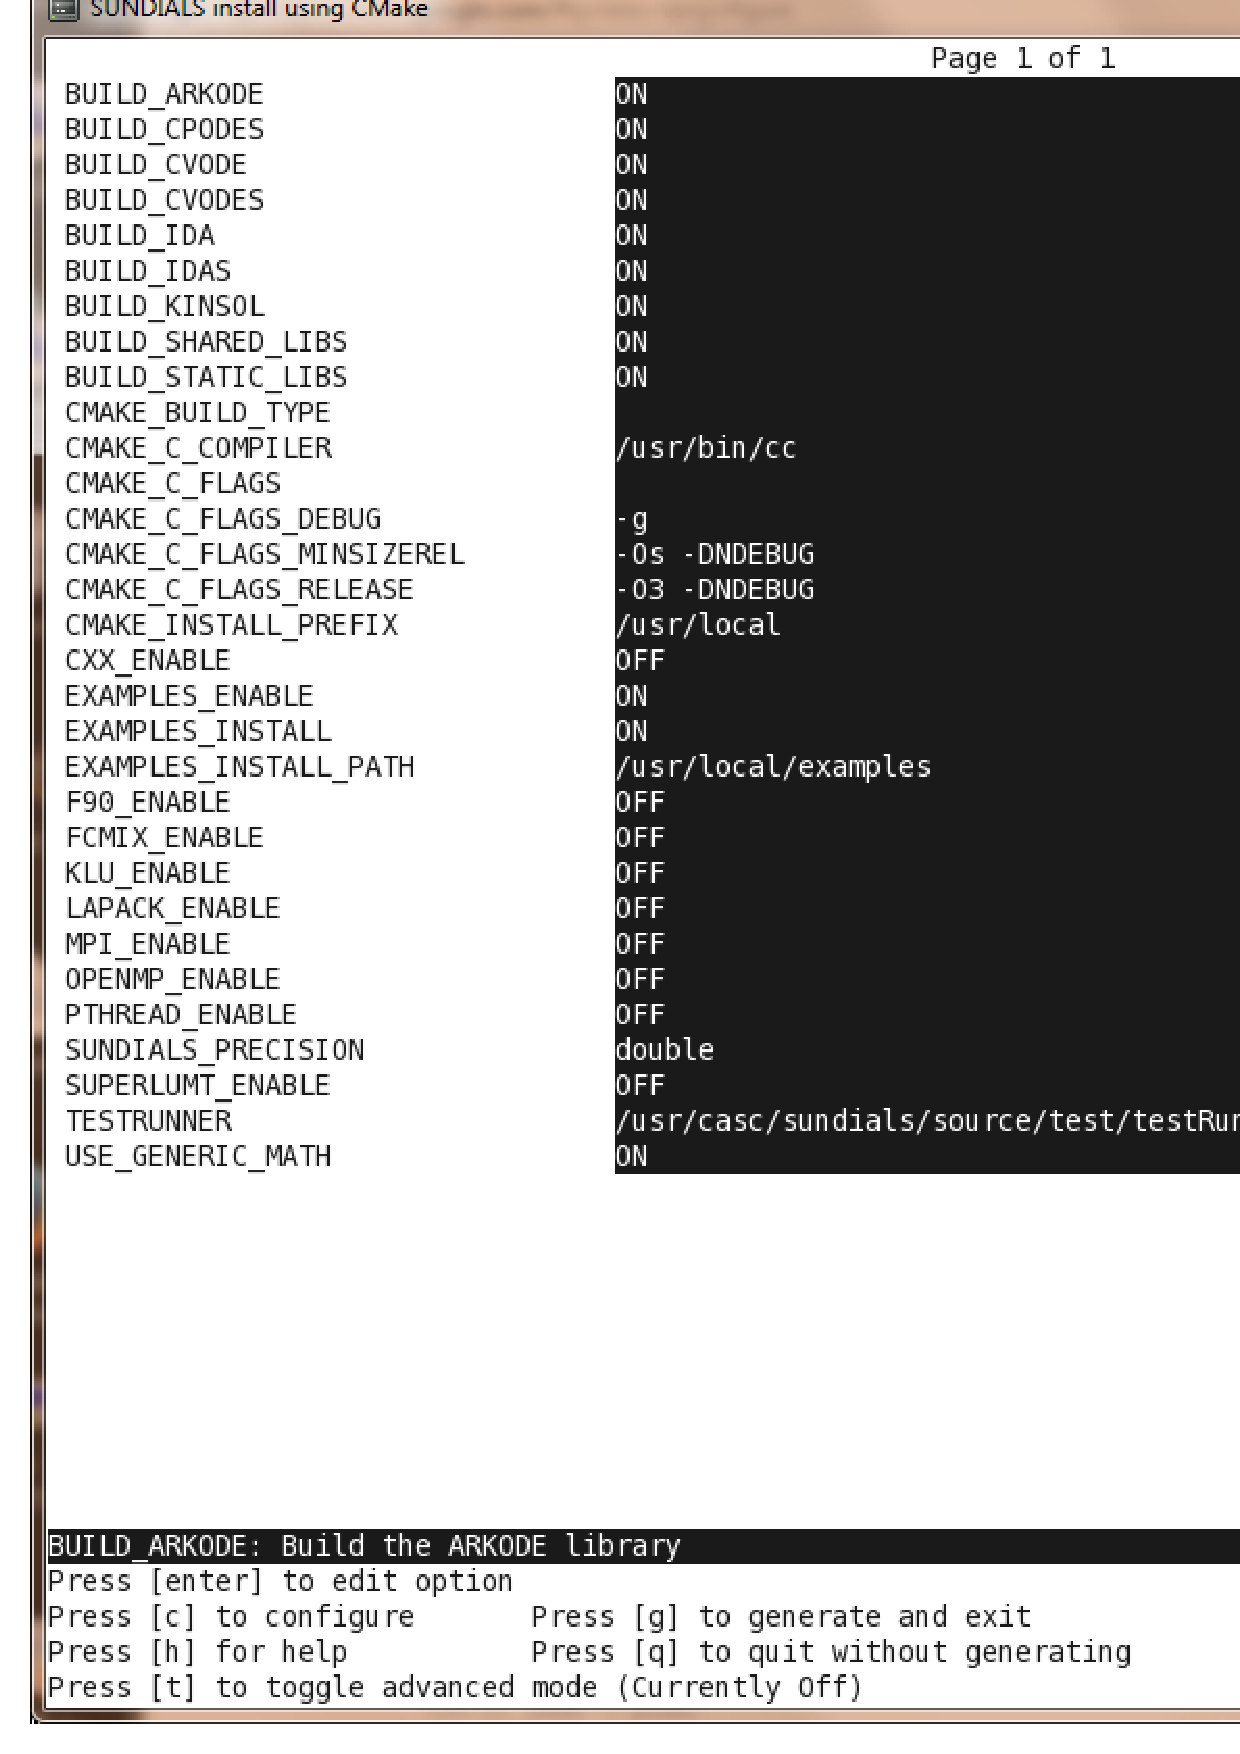
\includegraphics[width=\textwidth]{ccmakedefault}}}
\caption [Initial {\em ccmake} configuration screen]
{Default configuration screen. Note: Initial screen is empty.
To get this default configuration, press 'c' repeatedly (accepting default values denoted with asterisk)
until the 'g' option is available.}
\label{f:ccmakedefault}
\end{figure}

The default {\em instdir} for both {\sundials} and corresponding examples
can be changed by setting the \id{CMAKE\_INSTALL\_PREFIX} and
the \id{EXAMPLES\_INSTALL\_PATH} as shown in figure
\ref{f:ccmakeprefix}. 
\begin{figure}[!ht]
{\centerline{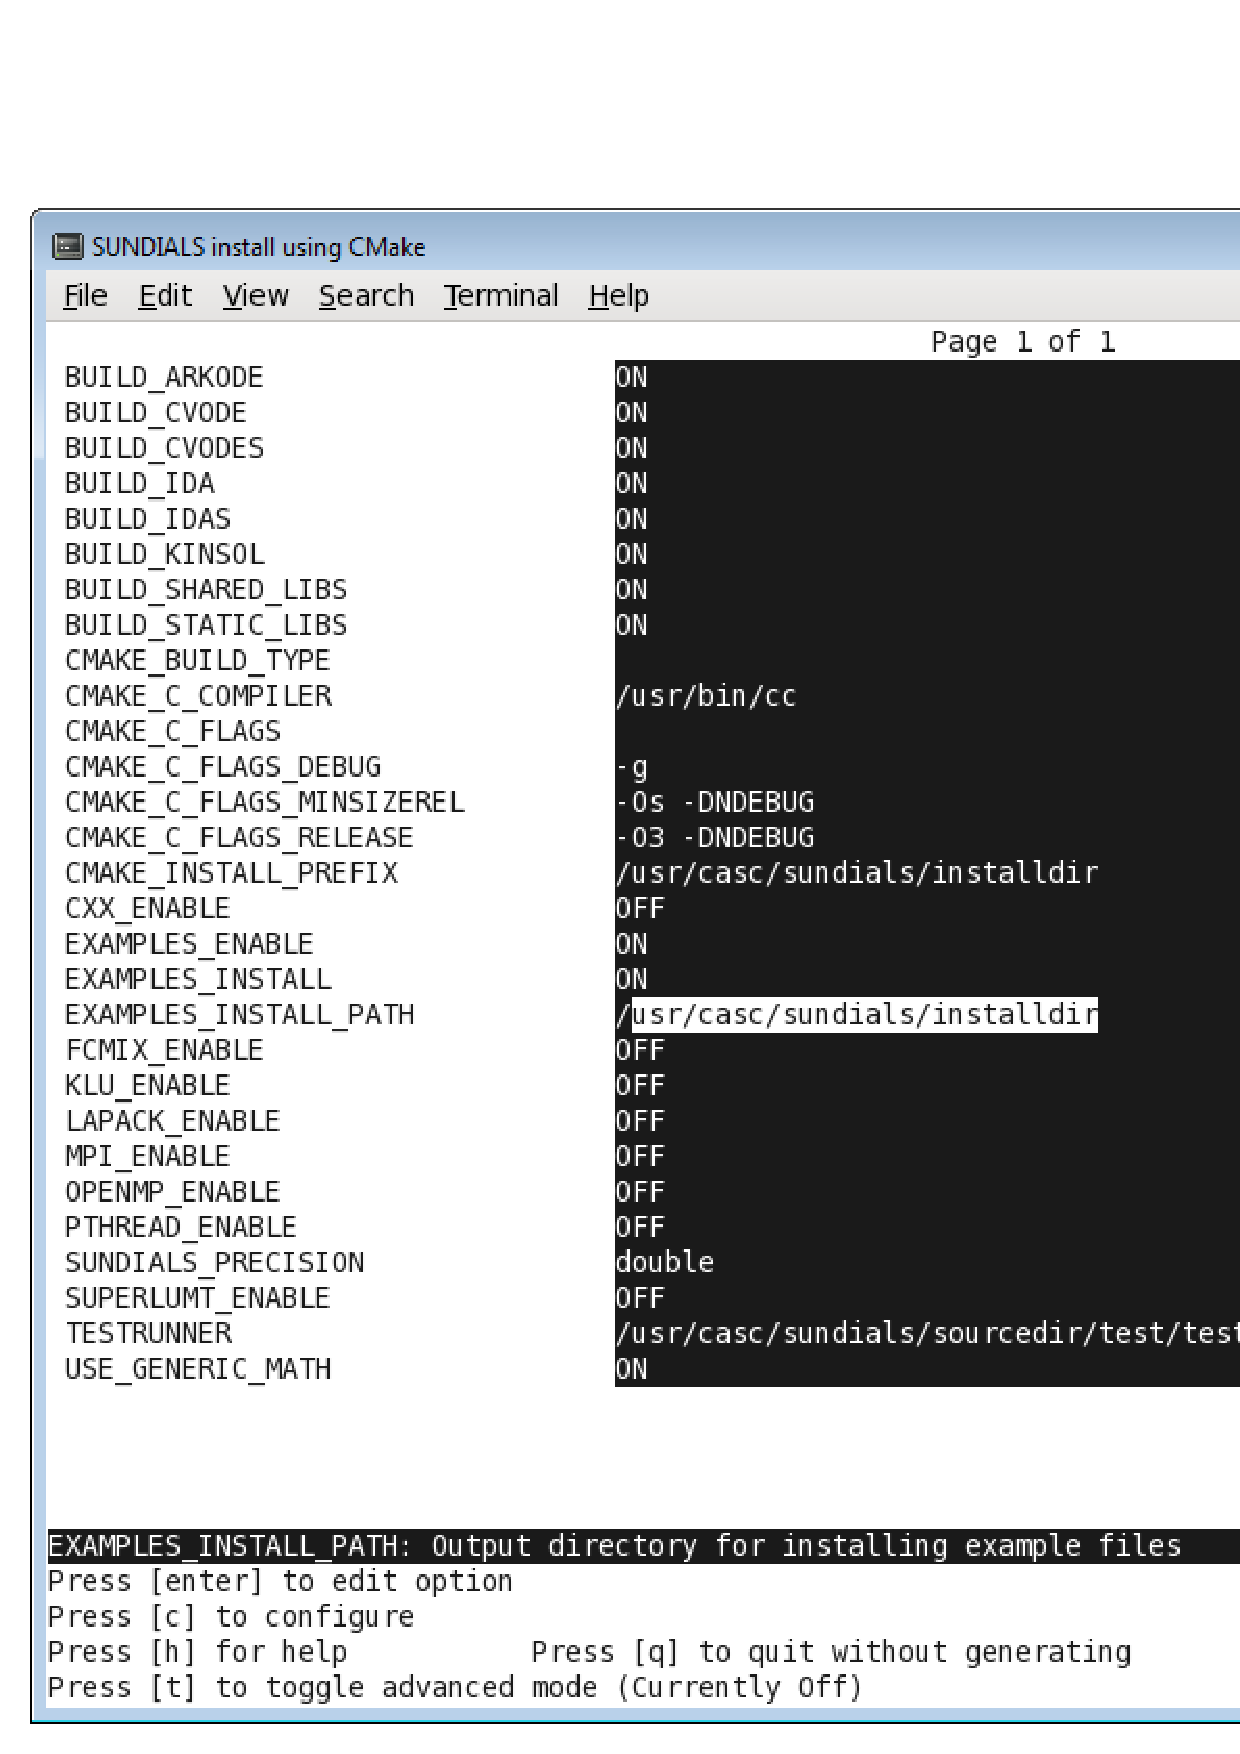
\includegraphics[width=\textwidth]{ccmakeprefix}}}
\caption [Changing the {\em instdir}]
{Changing the {\em instdir} for {\sundials} and
corresponding {\id examples} }
\label{f:ccmakeprefix}
\end{figure}

Pressing the (\id{g} key) will generate makefiles including all dependencies
and all rules to build {\sundials} on this system. 
Back at the command prompt, you can now run:

\begin{verbatim}
  % make
\end{verbatim}

To install {\sundials} in the installation directory specified in the configuration, simply run:

\begin{verbatim}
  % make install
\end{verbatim}

%%
%% *** NOTE: The TestRunner will not be distributed at this time.
%% *** Thus the following is commented out from the documentation.
%% TestRunner
%%
%\subsubsection*{Testing Installation}
%The distribution of {\sundials} includes several examples corresponding to the solvers to be
%installed. Also included in the source bundle is a test script: \id{testRunner}, configured by CMake
%to test the included examples.
%To run the tests, enter:

%\begin{verbatim}
%  % make test
%\end{verbatim}
%The output of \id{testRunner} should look similar to the screens in figure
%\ref{f:testrunner}. The success of each test is based on a line-by-line comparison of expected output files, bundled with the source code, with
%the output of the newly compiled examples. The file compare does allow some differences in rounding for float values.\\\\
%NOTE: Some tests may {\em fail} due to differences in machine architecture, compiler versions, third party libraries etc.{\warn}

%\begin{figure}[!ht]
%{\centerline{\includegraphics{figure=testrunnertop.eps,width=\textwidth}}}
%\vspace{3 mm}
%{\centerline{\includegraphics{figure=testrunnerbot.eps,width=\textwidth}}}
%\caption [Running {\em testRunner}]
%{Invoking {\em testRunner} with {\id make test} to execute all configured
%{\id examples} }
%\label{f:testrunner}
%\end{figure}

 
%%
%% Building from the command line
%%
\subsubsection*{Building from the command line}

Using CMake from the command line is simply a matter of specifying CMake variable settings
with the \id{cmake} command.  The following will build the default configuration:  

\begin{verbatim}
   % cmake -DCMAKE_INSTALL_PREFIX=/home/myname/sundials/instdir \
   > -DEXAMPLES_INSTALL_PATH=/home/myname/sundials/instdir/examples \
   > ../solverdir
   % make
   % make install
\end{verbatim}


\subsection{Configuration options (Unix/Linux)}\label{ss:configuration_options_nix}

A complete list of all available options for a CMake-based {\sundials}
configuration is provide below. Note that the default values shown are for 
a typical configuration on a Linux system and are provided as illustration only.

\begin{description}
\item[\id{BLAS\_ENABLE}] - 
  Enable BLAS support
  \\
  Default: OFF
  \\
  Note: Setting this option to ON will trigger additional CMake
  options. See additional information on building with BLAS enabled
  in \ref{ss:externallibs}.
\item[\id{BLAS\_LIBRARIES}] - 
  BLAS library
  \\
  Default: /usr/lib/libblas.so
  \\
  Note: CMake will search for libraries in your \id{LD\_LIBRARY\_PATH} prior
  to searching default system paths.
\item[\id{BUILD\_ARKODE}] - 
  Build the ARKODE library 
  \\
  Default: ON
\item[\id{BUILD\_CVODE}] - 
  Build the CVODE library 
  \\
  Default: ON
\item[\id{BUILD\_CVODES}] - 
  Build the CVODES library 
  \\
  Default: ON
\item[\id{BUILD\_IDA}] - 
   Build the IDA library 
  \\
   Default: ON
\item[\id{BUILD\_IDAS}] - 
  Build the IDAS library 
  \\
  Default: ON
\item[\id{BUILD\_KINSOL}] - 
  Build the KINSOL library 
  \\
  Default: ON
\item[\id{BUILD\_SHARED\_LIBS}] - 
  Build shared libraries
  \\
  Default: ON
\item[\id{BUILD\_STATIC\_LIBS}] - 
  Build static libraries
  \\
  Default: ON 
\item[\id{CMAKE\_BUILD\_TYPE}] -  
  Choose the type of build, options are: 
  \id{None} (CMAKE\_C\_FLAGS used), \id{Debug}, \id{Release},
  \id{RelWithDebInfo}, and \id{MinSizeRel}
  \\
  Default:
  \\
  Note: Specifying a build type will trigger the corresponding
  build type specific compiler flag options below which will be
  appended to the flags set by
  CMAKE\_{\textless}language{\textgreater}\_FLAGS. 
\item[\id{CMAKE\_C\_COMPILER}] - 
  C compiler
  \\
  Default: /usr/bin/cc 
\item[\id{CMAKE\_C\_FLAGS}] -  
  Flags for C compiler
  \\
  Default:
\item[\id{CMAKE\_C\_FLAGS\_DEBUG}] -      
  Flags used by the C compiler during debug builds
  \\
  Default: -g 
\item[\id{CMAKE\_C\_FLAGS\_MINSIZEREL}] -  
  Flags used by the C compiler during release minsize builds
  \\
  Default: -Os -DNDEBUG 
\item[\id{CMAKE\_C\_FLAGS\_RELEASE}] -    
  Flags used by the C compiler during release builds
  \\
  Default: -O3 -DNDEBUG 
\item[\id{CMAKE\_CXX\_COMPILER}] - 
  {\CPP} compiler
  \\
  Default: /usr/bin/c++
  \\
  Note: A {\CPP} compiler (and all related options) are only
  triggered if {\CPP} examples are enabled (\id{EXAMPLES\_ENABLE\_CXX}
  is ON). All {\sundials} solvers can be used from {\CPP} applications 
  by default without setting any additional configuration options.
\item[\id{CMAKE\_CXX\_FLAGS}] -
  Flags for {\CPP} compiler
  \\
  Default:
\item[\id{CMAKE\_CXX\_FLAGS\_DEBUG}] -
  Flags used by the {\CPP} compiler during debug builds
  \\
  Default: -g 
\item[\id{CMAKE\_CXX\_FLAGS\_MINSIZEREL}] -
  Flags used by the {\CPP} compiler during release minsize builds
  \\
  Default: -Os -DNDEBUG 
\item[\id{CMAKE\_CXX\_FLAGS\_RELEASE}] -
  Flags used by the {\CPP} compiler during release builds
  \\
  Default: -O3 -DNDEBUG
\item[\id{CMAKE\_Fortran\_COMPILER}] - 
  Fortran compiler
  \\
  Default: /usr/bin/gfortran
  \\
  Note: Fortran support (and all related options) are triggered only if
  either Fortran-C support is enabled (\id{FCMIX\_ENABLE} is ON) or
  BLAS/LAPACK support is enabled (\id{BLAS\_ENABLE} or \id{LAPACK\_ENABLE} is ON).
\item[\id{CMAKE\_Fortran\_FLAGS}] - 
  Flags for Fortran compiler
  \\
  Default:
\item[\id{CMAKE\_Fortran\_FLAGS\_DEBUG}] - 
  Flags used by the Fortran compiler during debug builds
  \\
  Default: -g
\item[\id{CMAKE\_Fortran\_FLAGS\_MINSIZEREL}] - 
  Flags used by the Fortran compiler during release minsize builds
  \\
  Default: -Os
\item[\id{CMAKE\_Fortran\_FLAGS\_RELEASE}] - 
  Flags used by the Fortran compiler during release builds
  \\
  Default: -O3
\item[\id{CMAKE\_INSTALL\_PREFIX}] -   
  Install path prefix, prepended onto install directories
  \\
  Default: /usr/local 
  \\
  Note: The user must have write access to the location specified through
  this option. Exported {\sundials} header files and libraries will be 
  installed under subdirectories \id{include} and \id{lib} of 
  \id{CMAKE\_INSTALL\_PREFIX}, respectively.
\item[\id{CUDA\_ENABLE}] -
  Build the {\sundials} {\cuda} vector module.
  \\
  Default: OFF
\item[\id{EXAMPLES\_ENABLE\_C}] -
  Build the {\sundials} {\CC} examples
  \\
  Default: ON
\item[\id{EXAMPLES\_ENABLE\_CUDA}] -
  Build the {\sundials} {\cuda} examples
  \\
  Default: OFF
  \\
  Note: You need to enable {\cuda} support to build these examples.
\item[\id{EXAMPLES\_ENABLE\_CXX}] -
  Build the {\sundials} {\CPP} examples
  \\
  Default: OFF
\item[\id{EXAMPLES\_ENABLE\_RAJA}] -
  Build the {\sundials} {\raja} examples
  \\
  Default: OFF
  \\
  Note: You need to enable {\cuda} and {\raja} support to build these examples.
\item[\id{EXAMPLES\_ENABLE\_F77}] -
  Build the {\sundials} Fortran77 examples
  \\
  Default: ON (if \id{FCMIX\_ENABLE} is ON)
\item[\id{EXAMPLES\_ENABLE\_F90}] -
  Build the {\sundials} Fortran90 examples
  \\
  Default: OFF
\item[\id{EXAMPLES\_INSTALL}] - 
  Install example files
  \\
  Default: ON
  \\
  Note: This option is triggered when any of the {\sundials}
  example programs are enabled \\
  (\id{EXAMPLES\_ENABLE\_$<$language$>$} is ON). If the user requires
  installation of example programs then the sources and sample output files
  for all {\sundials} modules that are currently enabled will be exported to
  the directory specified by \id{EXAMPLES\_INSTALL\_PATH}. A CMake configuration
  script will also be automatically generated and exported to the same directory.
  Additionally, if the configuration is done under a Unix-like system, makefiles
  for the compilation of the example programs (using the installed {\sundials} libraries)
  will be automatically generated and exported to the directory
  specified by \id{EXAMPLES\_INSTALL\_PATH}.
\item[\id{EXAMPLES\_INSTALL\_PATH}] - 
  Output directory for installing example files
  \\
  Default: /usr/local/examples
  \\
  Note: The actual default value for this option will be an \id{examples}
  subdirectory created under \id{CMAKE\_INSTALL\_PREFIX}.
\item[\id{FCMIX\_ENABLE}] - 
  Enable Fortran-C support   
  \\
  Default: OFF 
\item[\id{HYPRE\_ENABLE}] - 
  Enable \textit{hypre} support
  \\
  Default: OFF 
  \\
  Note: See additional information on building with \textit{hypre} enabled in
  \ref{ss:externallibs}. 
\item[\id{HYPRE\_INCLUDE\_DIR}] - 
  Path to \textit{hypre} header files
\item[\id{HYPRE\_LIBRARY\_DIR}] - 
  Path to \textit{hypre} installed library files
\item[\id{KLU\_ENABLE}] - 
  Enable KLU support
  \\
  Default: OFF 
  \\
  Note: See additional information on building with KLU enabled in
  \ref{ss:externallibs}. 
\item[\id{KLU\_INCLUDE\_DIR}] - 
  Path to SuiteSparse header files
\item[\id{KLU\_LIBRARY\_DIR}] - 
  Path to SuiteSparse installed library files
\item[\id{LAPACK\_ENABLE}] -  
  Enable LAPACK support
  \\
  Default: OFF
  \\
  Note: Setting this option to ON will trigger additional CMake
  options. See additional information on building with LAPACK enabled
  in \ref{ss:externallibs}.
\item[\id{LAPACK\_LIBRARIES}] - 
  LAPACK (and BLAS) libraries
  \\
  Default: /usr/lib/liblapack.so;/usr/lib/libblas.so
  \\
  Note: CMake will search for libraries in your \id{LD\_LIBRARY\_PATH} prior
  to searching default system paths.
\item[\id{MPI\_ENABLE}] -
  Enable MPI support (build the parallel nvector).
  \\
  Default: OFF 
  \\
  Note: Setting this option to ON will trigger several additional options
  related to MPI.
\item[\id{MPI\_C\_COMPILER}] -
  \id{mpicc} program
  \\
  Default: 
\item[\id{MPI\_CXX\_COMPILER}] -
  \id{mpicxx} program
  \\
  Default: 
  \\
  Note: This option is triggered only if MPI is enabled
  (\id{MPI\_ENABLE} is ON) and {\CPP} examples are enabled
  (\id{EXAMPLES\_ENABLE\_CXX} is ON). All {\sundials}
  solvers can be used from {\CPP} MPI applications by default
  without setting any additional configuration options other than
  \id{MPI\_ENABLE}.
\item[\id{MPI\_Fortran\_COMPILER}] -
  \id{mpif77} or \id{mpif90} program
  \\
  Default: 
  \\
  Note: This option is triggered only if MPI is enabled
  (\id{MPI\_ENABLE} is ON), Fortran-C support is enabled
  (\id{FCMIX\_ENABLE} is ON), and Fortran77 or Fortran90
  examples are enabled (\id{EXAMPLES\_ENABLE\_F77} or
  \id{EXAMPLES\_ENABLE\_F90} are ON).
\item[\id{MPIEXEC}] -
  Specify the executable for running MPI programs
  \\
  Default: \id{mpirun}
  \\
  Note: This option is triggered only if MPI is enabled
  (\id{MPI\_ENABLE} is ON).
  %% \\
  %% Note: This can either be set to \id{mpirun} for OpenMPI or \id{srun} if jobs are
  %% managed by \id{SLURM} - Simple Linux Utility for Resource Management as exists on
  %% LLNL's high performance computing clusters. 
\item[\id{OPENMP\_ENABLE}] -
  Enable OpenMP support (build the OpenMP nvector).
  \\
  Default: OFF 
\item[\id{PETSC\_ENABLE}] - 
  Enable PETSc support
  \\
  Default: OFF 
  \\
  Note: See additional information on building with PETSc enabled
  in \ref{ss:externallibs}.
\item[\id{PETSC\_INCLUDE\_DIR}] -
  Path to PETSc header files
\item[\id{PETSC\_LIBRARY\_DIR}] - 
  Path to PETSc installed library files
\item[\id{PTHREAD\_ENABLE}] -  
  Enable Pthreads support (build the Pthreads nvector).
  \\
  Default: OFF 
\item[\id{RAJA\_ENABLE}] - 
  Enable {\raja} support (build the {\raja} nvector).
  \\
  Default: OFF 
  \\
  Note: You need to enable {\cuda} in order to build the {\raja} vector module.
\item[\id{SUNDIALS\_F77\_FUNC\_CASE}] - \textbf{advanced option} -
  Specify the case to use in the Fortran name-mangling scheme, options
  are: \id{lower} or \id{upper}
  \\
  Default:
  \\
  Note: The build system will attempt to infer the Fortran
  name-mangling scheme using the Fortran compiler. This option should
  only be used if a Fortran compiler is not available or to override
  the inferred or default (\id{lower}) scheme if one can not be
  determined. If used, \id{SUNDIALS\_F77\_FUNC\_UNDERSCORES} must also
  be set.
\item[\id{SUNDIALS\_F77\_FUNC\_UNDERSCORES}] - \textbf{advanced option} -
  Specify the number of underscores to append in the Fortran
  name-mangling scheme, options are: \id{none}, \id{one}, or \id{two}
  \\
  Default:
  \\
  Note: The build system will attempt to infer the Fortran
  name-mangling scheme using the Fortran compiler. This option should
  only be used if a Fortran compiler is not available or to override
  the inferred or default (\id{one}) scheme if one can not be
  determined. If used, \id{SUNDIALS\_F77\_FUNC\_CASE} must also be set.
\item[\id{SUNDIALS\_INDEX\_TYPE}] - 
  Integer type used for {\sundials} indices, options are: \id{int32\_t} or \id{int64\_t}
  \\
  Default: \id{int64\_t}
\item[\id{SUNDIALS\_PRECISION}] -   
  Precision used in {\sundials}, options are: \id{double}, \id{single}, or \id{extended}
  \\
  Default: \id{double}
\item[\id{SUPERLUMT\_ENABLE}] - 
  Enable SuperLU\_MT support   
  \\
  Default: OFF 
  \\
  Note: See additional information on building with SuperLU\_MT enabled
  in \ref{ss:externallibs}.
\item[\id{SUPERLUMT\_INCLUDE\_DIR}] - 
  Path to SuperLU\_MT header files (typically SRC directory)
\item[\id{SUPERLUMT\_LIBRARY\_DIR}] - 
  Path to SuperLU\_MT installed library files
\item[\id{SUPERLUMT\_THREAD\_TYPE}] - 
  Must be set to Pthread or OpenMP
  \\
  Default: Pthread
\item[\id{USE\_GENERIC\_MATH}] -   
  Use generic (stdc) math libraries
  \\
  Default: ON 
\end{description}

\subsubsection*{xSDK Configuration Options}

{\sundials} supports CMake configuration options defined by the
Extreme-scale Scientific Software Development Kit (xSDK) community
policies (see {\tt https://xsdk.info} for more information). xSDK
CMake options are unused by default but may be activated by setting
\id{USE\_XSDK\_DEFAULTS} to ON.

{\warn} When xSDK options are active, they will overwrite the
corresponding {\sundials} option and may have different default values
(see details below). As such the equivalent {\sundials} options should
not be used when configuring with xSDK options. In the GUI front end
to CMake (\id{ccmake}), setting \id{USE\_XSDK\_DEFAULTS} to ON will
hide the corresponding {\sundials} options as advanced CMake variables.
During configuration, messages are output detailing
which xSDK flags are active and the equivalent {\sundials} options
that are replaced. Below is a complete list xSDK options and the
corresponding {\sundials} options if applicable.

\begin{description}
\item[\id{TPL\_BLAS\_LIBRARIES}] - 
  BLAS library
  \\
  Default: /usr/lib/libblas.so
  \\
  {\sundials} equivalent: \id{BLAS\_LIBRARIES}
  \\
  Note: CMake will search for libraries in your \id{LD\_LIBRARY\_PATH} prior
  to searching default system paths.
\item[\id{TPL\_ENABLE\_BLAS}] - 
  Enable BLAS support
  \\
  Default: OFF
  \\
  {\sundials} equivalent: \id{BLAS\_ENABLE}
\item[\id{TPL\_ENABLE\_HYPRE}] - 
  Enable \textit{hypre} support
  \\
  Default: OFF
  \\
  {\sundials} equivalent: \id{HYPRE\_ENABLE}
\item[\id{TPL\_ENABLE\_KLU}] - 
  Enable KLU support
  \\
  Default: OFF
  \\
  {\sundials} equivalent: \id{KLU\_ENABLE}
\item[\id{TPL\_ENABLE\_PETSC}] - 
  Enable PETSc support
  \\
  Default: OFF
  \\
  {\sundials} equivalent: \id{PETSC\_ENABLE}
\item[\id{TPL\_ENABLE\_LAPACK}] - 
  Enable LAPACK support
  \\
  Default: OFF
  \\
  {\sundials} equivalent: \id{LAPACK\_ENABLE}
\item[\id{TPL\_ENABLE\_SUPERLUMT}] - 
  Enable SuperLU\_MT support
  \\
  Default: OFF
  \\
  {\sundials} equivalent: \id{SUPERLUMT\_ENABLE}
\item[\id{TPL\_HYPRE\_INCLUDE\_DIRS}] - 
  Path to \textit{hypre} header files
  \\
  {\sundials} equivalent: \id{HYPRE\_INCLUDE\_DIR}
\item[\id{TPL\_HYPRE\_LIBRARIES}] - 
  \textit{hypre} library
  \\
  {\sundials} equivalent: N/A
\item[\id{TPL\_KLU\_INCLUDE\_DIRS}] - 
  Path to KLU header files
  \\
  {\sundials} equivalent: \id{KLU\_INCLUDE\_DIR}
\item[\id{TPL\_KLU\_LIBRARIES}] - 
  KLU library
  \\
  {\sundials} equivalent: N/A
\item[\id{TPL\_LAPACK\_LIBRARIES}] - 
  LAPACK (and BLAS) libraries
  \\
  Default: /usr/lib/liblapack.so;/usr/lib/libblas.so
  \\
  {\sundials} equivalent: \id{LAPACK\_LIBRARIES}
  \\
  Note: CMake will search for libraries in your \id{LD\_LIBRARY\_PATH} prior
  to searching default system paths.
\item[\id{TPL\_PETSC\_INCLUDE\_DIRS}] - 
  Path to PETSc header files
  \\
  {\sundials} equivalent: \id{PETSC\_INCLUDE\_DIR}
\item[\id{TPL\_PETSC\_LIBRARIES}] - 
  PETSc library
  \\
  {\sundials} equivalent: N/A
\item[\id{TPL\_SUPERLUMT\_INCLUDE\_DIRS}] - 
  Path to SuperLU\_MT header files
  \\
  {\sundials} equivalent: \id{SUPERLUMT\_INCLUDE\_DIR}
\item[\id{TPL\_SUPERLUMT\_LIBRARIES}] - 
  SuperLU\_MT library
  \\
  {\sundials} equivalent: N/A
\item[\id{TPL\_SUPERLUMT\_THREAD\_TYPE}] - 
  SuperLU\_MT library thread type
  \\
  {\sundials} equivalent: \id{SUPERLUMT\_THREAD\_TYPE}
\item[\id{USE\_XSDK\_DEFAULTS}] - 
  Enable xSDK default configuration settings
  \\
  Default: OFF
  \\
  {\sundials} equivalent: N/A
  \\
  Note: Enabling xSDK defaults also sets \id{CMAKE\_BUILD\_TYPE} to \id{Debug}
\item[\id{XSDK\_ENABLE\_FORTRAN}] -
  Enable {\sundials} Fortran interface
  \\
  Default: OFF
  \\
  {\sundials} equivalent: \id{FCMIX\_ENABLE}
\item[\id{XSDK\_INDEX\_SIZE}] -
  Integer size (bits) used for indices in {\sundials}, options are: \id{32} or \id{64}
  \\
  Default: \id{32}
  \\
  {\sundials} equivalent: \id{SUNDIALS\_INDEX\_TYPE}
\item[\id{XSDK\_PRECISION}] -
  Precision used in {\sundials}, options are: \id{double}, \id{single}, or \id{quad}
  \\
  Default: \id{double}
  \\
  {\sundials} equivalent: \id{SUNDIALS\_PRECISION}
\end{description}



%%===============================================================================

\subsection{Configuration examples}

The following examples will help demonstrate usage of the CMake configure options.

\noindent To configure {\sundials} using the default C and Fortran compilers,
and default \id{mpicc} and \id{mpif77} parallel compilers, 
enable compilation of examples, and install libraries, headers, and
example sources under subdirectories of
\id{/home/myname/sundials/}, use:

\begin{verbatim}
   % cmake \
   > -DCMAKE_INSTALL_PREFIX=/home/myname/sundials/instdir \
   > -DEXAMPLES_INSTALL_PATH=/home/myname/sundials/instdir/examples \
   > -DMPI_ENABLE=ON \
   > -DFCMIX_ENABLE=ON \
   > /home/myname/sundials/solverdir
   %
   % make install
   % 
\end{verbatim}

\noindent To disable installation of the examples, use:
\begin{verbatim}
   % cmake \
   > -DCMAKE_INSTALL_PREFIX=/home/myname/sundials/instdir \
   > -DEXAMPLES_INSTALL_PATH=/home/myname/sundials/instdir/examples \
   > -DMPI_ENABLE=ON \
   > -DFCMIX_ENABLE=ON \
   > -DEXAMPLES_INSTALL=OFF \
   > /home/myname/sundials/solverdir
   %
   % make install
   % 
\end{verbatim}

%%===============================================================================
\subsection{Working with external Libraries} \label{ss:externallibs}

The {\sundials} suite contains many options to enable implementation flexibility
when developing solutions. The following are some notes addressing specific configurations
when using the supported third party libraries.
When building {\sundials} as a shared library external libraries any
used with {\sundials} must also be build as a shared library or as a
static library compiled with the \id{-fPIC} flag.{\warn}

\subsubsection*{Building with BLAS}
{\sundials} does not utilize BLAS directly but it may be needed by other
external libraries that {\sundials} can be built with (e.g. LAPACK,
PETSc, SuperLU\_MT, etc.). To enable BLAS, set the \id{BLAS\_ENABLE}
option to \id{ON}. If the directory containing the BLAS library is in
the \id{LD\_LIBRARY\_PATH} environment variable, CMake will set the
\id{BLAS\_LIBRARIES} variable accordingly, otherwise CMake will
attempt to find the BLAS library in standard system locations. To
explicitly tell CMake what libraries to use, the \id{BLAS\_LIBRARIES}
variable can be set to the desired library. Example:
\begin{verbatim}
   % cmake \
   > -DCMAKE_INSTALL_PREFIX=/home/myname/sundials/instdir \
   > -DEXAMPLES_INSTALL_PATH=/home/myname/sundials/instdir/examples \
   > -DBLAS_ENABLE=ON \
   > -DBLAS_LIBRARIES=/myblaspath/lib/libblas.so \
   > -DSUPERLUMT_ENABLE=ON \
   > -DSUPERLUMT_INCLUDE_DIR=/mysuperlumtpath/SRC
   > -DSUPERLUMT_LIBRARY_DIR=/mysuperlumtpath/lib
   > /home/myname/sundials/solverdir
   %
   % make install
   % 
\end{verbatim}
{\warn}When allowing CMake to automatically locate the LAPACK library,
CMake \textit{may} also locate the corresponding BLAS library.

If a working Fortran compiler is not available to infer the Fortran
name-mangling scheme, the options \id{SUNDIALS\_F77\_FUNC\_CASE} and
\id{SUNDIALS\_F77\_FUNC\_UNDERSCORES} \textit{must} be set in order to
bypass the check for a Fortran compiler and define the name-mangling
scheme. The defaults for these options in earlier versions of
{\sundials} were \id{lower} and \id{one} respectively.


\subsubsection*{Building with LAPACK}
To enable LAPACK, set the \id{LAPACK\_ENABLE} option to \id{ON}.
If the directory containing the LAPACK library is in the
\id{LD\_LIBRARY\_PATH} environment variable, CMake will set the
\id{LAPACK\_LIBRARIES} variable accordingly, otherwise CMake will
attempt to find the LAPACK library in standard system locations. To
explicitly tell CMake what library to use, the \id{LAPACK\_LIBRARIES}
variable can be set to the desired libraries. {\warn}When setting
the LAPACK location explicitly the location of the corresponding BLAS
library will also need to be set. Example:
\begin{verbatim}
   % cmake \
   > -DCMAKE_INSTALL_PREFIX=/home/myname/sundials/instdir \
   > -DEXAMPLES_INSTALL_PATH=/home/myname/sundials/instdir/examples \
   > -DBLAS_ENABLE=ON \
   > -DBLAS_LIBRARIES=/mylapackpath/lib/libblas.so \
   > -DLAPACK_ENABLE=ON \
   > -DLAPACK_LIBRARIES=/mylapackpath/lib/liblapack.so \
   > /home/myname/sundials/solverdir
   %
   % make install
   % 
\end{verbatim}
{\warn}When allowing CMake to automatically locate the LAPACK library,
CMake \textit{may} also locate the corresponding BLAS library.

If a working Fortran compiler is not available to infer the Fortran
name-mangling scheme, the options \id{SUNDIALS\_F77\_FUNC\_CASE} and
\id{SUNDIALS\_F77\_FUNC\_UNDERSCORES} \textit{must} be set in order to
bypass the check for a Fortran compiler and define the name-mangling
scheme. The defaults for these options in earlier versions of
{\sundials} were \id{lower} and \id{one} respectively.

\subsubsection*{Building with KLU}
The KLU libraries are part of SuiteSparse, a suite of sparse matrix software,
available from the Texas A\&M University website: {\tt http://faculty.cse.tamu.edu/davis/suitesparse.html}.
{\sundials} has been tested with SuiteSparse version 4.5.3.
To enable KLU, set \id{KLU\_ENABLE} to \id{ON}, set \id{KLU\_INCLUDE\_DIR} to the \id{include}
path of the KLU installation and set \id{KLU\_LIBRARY\_DIR} to the \id{lib} path of the KLU installation.
The CMake configure will result in populating the following variables: \id{AMD\_LIBRARY},
\id{AMD\_LIBRARY\_DIR}, \id{BTF\_LIBRARY}, \id{BTF\_LIBRARY\_DIR},
\id{COLAMD\_LIBRARY}, \id{COLAMD\_LIBRARY\_DIR}, and
\newline\id{KLU\_LIBRARY}.

\subsubsection*{Building with SuperLU\_MT}
The SuperLU\_MT libraries are available for download from the Lawrence Berkeley National Laboratory website:
{\tt http://crd-legacy.lbl.gov/$\sim$xiaoye/SuperLU/\#superlu\_mt}. 
{\sundials} has been tested with SuperLU\_MT version 3.1. 
To enable SuperLU\_MT, set  \id{SUPERLUMT\_ENABLE} to \id{ON}, set \id{SUPERLUMT\_INCLUDE\_DIR}
to the \id{SRC} path of the SuperLU\_MT installation, and set the variable
\newline\id{SUPERLUMT\_LIBRARY\_DIR} to the \id{lib} path of the SuperLU\_MT installation.
At the same time, the variable
\id{SUPERLUMT\_THREAD\_TYPE} must be set to either \id{Pthread} or \id{OpenMP}.

\noindent Do not mix thread types when building {\sundials} solvers.
If threading is enabled for {\sundials} by having either \id{OPENMP\_ENABLE} or \id{PTHREAD\_ENABLE} set to \id{ON}
then SuperLU\_MT should be set to use the same threading type.{\warn}

\subsubsection*{Building with PETSc}
The PETSc libraries are available for download from the Argonne National Laboratory website:
{\tt http://www.mcs.anl.gov/petsc}. 
{\sundials} has been tested with PETSc version 3.7.2. 
To enable PETSc, set  \id{PETSC\_ENABLE} to \id{ON}, set \id{PETSC\_INCLUDE\_DIR}
to the \id{include} path of the PETSc installation, and set the variable
\id{PETSC\_LIBRARY\_DIR} to the \id{lib} path of the PETSc installation.


\subsubsection*{Building with \textit{hypre}}
The \textit{hypre} libraries are available for download from the Lawrence Livermore
National Laboratory website: {\tt http://computation.llnl.gov/projects/hypre}.
%{\tt http://computation.llnl.gov/projects/hypre-scalable-linear-solvers-multigrid-methods}.
{\sundials} has been tested with \textit{hypre} version 2.11.1. 
To enable \textit{hypre}, set  \id{HYPRE\_ENABLE} to \id{ON}, set \id{HYPRE\_INCLUDE\_DIR}
to the \id{include} path of the \textit{hypre} installation, and set the variable
\id{HYPRE\_LIBRARY\_DIR} to the \id{lib} path of the \textit{hypre} installation.

\subsubsection*{Building with CUDA}
{\sundials} {\cuda} modules and examples have been tested with version 8.0 of the 
{\cuda} toolkit. To build them, you need to install the Toolkit and compatible
NVIDIA drivers. Both are available for download from the NVIDIA website:
{\tt https://developer.nvidia.com/cuda-downloads}. To enable {\cuda}, 
set \id{CUDA\_ENABLE} to \id{ON}. If {\cuda} is installed in a
nonstandard location, you may be prompted to set the variable
\id{CUDA\_TOOLKIT\_ROOT\_DIR} with your {\cuda} Toolkit installation
path. To enable {\cuda} examples, set \id{EXAMPLES\_ENABLE\_CUDA} to \id{ON}.

\subsubsection*{Building with RAJA}
{\raja} is a performance portability layer developed by Lawrence
Livermore National Laboratory and can be obtained from {\tt https://github.com/LLNL/RAJA}.
{\sundials} {\raja} modules and examples have been tested with {\raja}
version 0.3. Building {\sundials} {\raja} modules requires a
{\cuda}-enabled {\raja} installation. To enable {\raja}, set
\id{CUDA\_ENABLE} and \id{RAJA\_ENABLE} to \id{ON}. If {\raja} is
installed in a nonstandard location you will be prompted to set the
variable \id{RAJA\_DIR} with the path to the {\raja} CMake
configuration file. To enable building the {\raja} examples set
\id{EXAMPLES\_ENABLE\_RAJA} to \id{ON}.

\subsection{Testing the build and installation}

If {\sundials} was configured with
\id{EXAMPLES\_ENABLE\_$<$language$>$} options to \id{ON}, then a set of
regression tests can be run after building with the \id{make} command
by running: 
\begin{verbatim}
  % make test
\end{verbatim}
Additionally, if \id{EXAMPLES\_INSTALL} was also set to \id{ON}, then
a set of smoke tests can be run after installing with the \id{make install} 
command by running:
\begin{verbatim}
  % make test_install
\end{verbatim}

%%===============================================================================
\section{Building and Running Examples}
%%===============================================================================
Each of the {\sundials} solvers is distributed with a set of examples
demonstrating basic usage. To build and install the examples, set at
least of the \id{EXAMPLES\_ENABLE\_$<$language$>$} options to \id{ON}, and
set \id{EXAMPLES\_INSTALL} to \id{ON}.
Specify the installation path for the examples with the variable \id{EXAMPLES\_INSTALL\_PATH}. CMake will generate
\id{CMakeLists.txt} configuration files (and \id{Makefile} files if on Linux/Unix) that reference the
{\em installed} {\sundials} headers and libraries.

Either the \id{CMakeLists.txt} file or the traditional \id{Makefile} may be used to build the examples
as well as serve as a template for creating user developed solutions.
To use the supplied \id{Makefile} simply run \id{make} to compile and generate the executables.
To use CMake from within the installed example directory, run \id{cmake} (or \id{ccmake} to use the GUI)
followed by \id{make} to compile the example code.
Note that if CMake is used, it will overwrite the traditional \id{Makefile} with a new CMake-generated \id{Makefile}.
The resulting output from running the examples can be compared with example output bundled
in the {\sundials} distribution.

\noindent NOTE: There will potentially be differences in the output due to machine architecture, compiler versions,
use of third party libraries etc.{\warn} 


%%===============================================================================
\section{Configuring, building, and installing  on Windows}\label{s:cmake_windows}
%%===============================================================================
CMake can also be used to build {\sundials} on Windows. To build {\sundials} for
use with Visual Studio the following steps should be performed:
\begin{enumerate}
\item Unzip the downloaded tar file(s) into a directory. This will be the {\em solverdir} 
\item Create a separate {\em builddir}
\item Open a Visual Studio Command Prompt and cd to {\em builddir}
\item Run cmake-gui ../{\em solverdir}
\begin{enumerate}
\item Hit Configure
\item Check/Uncheck solvers to be built
\item Change CMAKE\_INSTALL\_PREFIX to {\em instdir}
\item Set other options as desired
\item Hit Generate
\end{enumerate}
\item Back in the VS Command Window:
\begin{enumerate}
\item Run msbuild ALL\_BUILD.vcxproj
\item Run msbuild INSTALL.vcxproj
\end{enumerate} 
\end{enumerate}

\noindent The resulting libraries will be in the {\em instdir}.
\noindent The {\sundials} project can also now be opened in Visual Studio.
Double click on the ALL\_BUILD.vcxproj file to open the project.
Build the whole {\em solution} to create the {\sundials} libraries.
To use the {\sundials} libraries in your own projects, you must
set the include directories for your project,
add the {\sundials} libraries to your project solution,
and set the {\sundials} libraries as dependencies for your project.

%%===============================================================================
\section{Installed libraries and exported header files}
%%===============================================================================

Using the CMake {\sundials} build system, the command
\begin{verbatim}
   % make install
\end{verbatim}
will install the libraries under {\em libdir} and the public header
files under {\em includedir}. The values for these directories are
{\em instdir}\id{/lib} and {\em instdir}\id{/include},
respectively. The location can be changed by setting the CMake variable \id{CMAKE\_INSTALL\_PREFIX}.
Although all installed libraries reside under {\em libdir}\id{/lib}, the public header files
are further organized into subdirectories under {\em includedir}\id{/include}.

The installed libraries and exported header files are listed for
reference in Table \ref{t:sundials_files}.
The file extension .{\em lib}
is typically \id{.so} for shared libraries and \id{.a} for static libraries.
Note that, in the Tables, names are relative to {\em libdir}
for libraries and to {\em includedir} for header files.

A typical user program need not explicitly include any of the shared
{\sundials} header files from under the {\em includedir}\id{/include}\id{/sundials}
directory since they are explicitly included by the appropriate solver
header files ({\em e.g.}, \id{cvode\_dense.h} includes
\id{sundials\_dense.h}). However, it is both legal and safe to do so,
and would be useful, for example, if the functions declared in \id{sundials\_dense.h} 
are to be used in building a preconditioner.

%---------------------------------------------------------------------------
% Table of installed files
%---------------------------------------------------------------------------

\newlength{\colLenOne}
\settowidth{\colLenOne}{{\sunlinsollapdense}}

\newlength{\colLenTwo}
\settowidth{\colLenTwo}{Header files}

\newlength{\colLenThree}
\setlength{\colLenThree}{\textwidth}
\addtolength{\colLenThree}{-0.5in}
\addtolength{\colLenThree}{-\colLenOne}
\addtolength{\colLenThree}{-\colLenTwo}

%\caption{{\sundials} libraries and header files (cont.)}\label{t:sundials_files2}

\tablecaption{{\sundials} libraries and header files}\label{t:sundials_files}
\tablefirsthead{\hline}
\tablehead{\hline \multicolumn{4}{|l|}{\small\slshape continued from last page} \\
           \hline}
\tabletail{\hline \multicolumn{4}{|r|}{\small\slshape continued on next page} \\ \hline}
\begin{xtabular}{|p{\colLenOne}|p{\colLenTwo}|p{0.5\colLenThree} p{0.5\colLenThree}|}

%% --------------------------------------------------
{\shared}
 & Libraries    & n/a  & \\
\cline{2-4}
 & Header files & sundials/sundials\_config.h        & sundials/sundials\_fconfig.h  \\
 &              & sundials/sundials\_types.h         & sundials/sundials\_math.h     \\
 &              & sundials/sundials\_nvector.h       & sundials/sundials\_fnvector.h \\
 &              & sundials/sundials\_iterative.h     & sundials/sundials\_direct.h   \\
 &              & sundials/sundials\_dense.h         & sundials/sundials\_band.h     \\
 &              & sundials/sundials\_matrix.h        & sundials/sundials\_version.h  \\
 &              & sundials/sundials\_linearsolver.h  & \\
\hline
%% --------------------------------------------------
{\nvecs}
 & Libraries    & libsundials\_nvecserial.{\em lib} & libsundials\_fnvecserial.a \\ 
\cline{2-4}
 & Header files & nvector/nvector\_serial.h         & \\ 
\hline
%% --------------------------------------------------
{\nvecp}
 & Libraries    & libsundials\_nvecparallel.{\em lib} & libsundials\_fnvecparallel.a \\
\cline{2-4}
 & Header files & nvector/nvector\_parallel.h         & \\
\hline
%% --------------------------------------------------
{\nvecopenmp}
 & Libraries    & libsundials\_nvecopenmp.{\em lib} & libsundials\_fnvecopenmp.a \\ 
\cline{2-4}
 & Header files & nvector/nvector\_openmp.h         & \\ 
\hline
%% --------------------------------------------------
{\nvecpthreads}
 & Libraries    & libsundials\_nvecpthreads.{\em lib} & libsundials\_fnvecpthreads.a \\ 
\cline{2-4}
 & Header files & nvector/nvector\_pthreads.h         & \\ 
\hline
%% --------------------------------------------------
{\nvecph}
 & Libraries    & libsundials\_nvecparhyp.{\em lib} & \\
\cline{2-4}
 & Header files & nvector/nvector\_parhyp.h         & \\ 
\hline
%% --------------------------------------------------
{\nvecpetsc}
 & Libraries    & libsundials\_nvecpetsc.{\em lib} & \\ 
\cline{2-4}
 & Header files & nvector/nvector\_petsc.h         & \\ 
\hline
%% --------------------------------------------------
{\nveccuda}
 & Libraries    & libsundials\_nveccuda.{\em lib}     & \\ 
\cline{2-4}
 & Header files & nvector/nvector\_cuda.h             & \\
 &              & nvector/cuda/ThreadPartitioning.hpp & \\
 &              & nvector/cuda/Vector.hpp             & \\
 &              & nvector/cuda/VectorKernels.cuh      & \\
\hline
%% --------------------------------------------------
{\nvecraja}
 & Libraries    & libsundials\_nvecraja.{\em lib} & \\ 
\cline{2-4}
 & Header files & nvector/nvector\_raja.h         & \\
 &              & nvector/raja/Vector.hpp         & \\
\hline
%% --------------------------------------------------
{\sunmatband}
 & Libraries    & libsundials\_sunmatrixband.{\em lib} & \\ 
 &              & libsundials\_fsunmatrixband.a        & \\ 
\cline{2-4}
 & Header files & sunmatrix/sunmatrix\_band.h          & \\ 
\hline
%% --------------------------------------------------
{\sunmatdense}
 & Libraries    & libsundials\_sunmatrixdense.{\em lib} & \\
 &              & libsundials\_fsunmatrixdense.a        & \\
\cline{2-4}
 & Header files & sunmatrix/sunmatrix\_dense.h          & \\
\hline
%% --------------------------------------------------
{\sunmatsparse}
 & Libraries    & libsundials\_sunmatrixsparse.{\em lib} & \\ 
 &              & libsundials\_fsunmatrixsparse.a        & \\ 
\cline{2-4}
 & Header files & sunmatrix/sunmatrix\_sparse.h          & \\ 
\hline
%% --------------------------------------------------
{\sunlinsolband}
 & Libraries    & libsundials\_sunlinsolband.{\em lib} & \\ 
 &              & libsundials\_fsunlinsolband.a        & \\ 
\cline{2-4}
 & Header files & sunlinsol/sunlinsol\_band.h          & \\ 
\hline
%% --------------------------------------------------
{\sunlinsoldense}
 & Libraries    & libsundials\_sunlinsoldense.{\em lib} & \\ 
 &              & libsundials\_fsunlinsoldense.a        & \\ 
\cline{2-4}
 & Header files & sunlinsol/sunlinsol\_dense.h          & \\ 
\hline
%% --------------------------------------------------
{\sunlinsolklu}
 & Libraries    & libsundials\_sunlinsolklu.{\em lib} & \\ 
 &              & libsundials\_fsunlinsolklu.a        & \\ 
\cline{2-4}
 & Header files & sunlinsol/sunlinsol\_klu.h          & \\ 
\hline
%% --------------------------------------------------
{\sunlinsollapband}
 & Libraries    & libsundials\_sunlinsollapackband.{\em lib} & \\ 
 &              & libsundials\_fsunlinsollapackband.a        & \\ 
\cline{2-4}
 & Header files & sunlinsol/sunlinsol\_lapackband.h          & \\ 
\hline
%% --------------------------------------------------
{\sunlinsollapdense}
 & Libraries    & libsundials\_sunlinsollapackdense.{\em lib} & \\ 
 &              & libsundials\_fsunlinsollapackdense.a        & \\ 
\cline{2-4}
 & Header files & sunlinsol/sunlinsol\_lapackdense.h          & \\ 
\hline
%% --------------------------------------------------
{\sunlinsolpcg}
 & Libraries    & libsundials\_sunlinsolpcg.{\em lib} & \\ 
 &              & libsundials\_fsunlinsolpcg.a        & \\ 
\cline{2-4}
 & Header files & sunlinsol/sunlinsol\_pcg.h          & \\ 
\hline
%% --------------------------------------------------
{\sunlinsolspbcgs}
 & Libraries    & libsundials\_sunlinsolspbcgs.{\em lib} & \\ 
 &              & libsundials\_fsunlinsolspbcgs.a        & \\ 
\cline{2-4}
 & Header files & sunlinsol/sunlinsol\_spbcgs.h          & \\ 
\hline
%% --------------------------------------------------
{\sunlinsolspfgmr}
 & Libraries    & libsundials\_sunlinsolspfgmr.{\em lib} & \\ 
 &              & libsundials\_fsunlinsolspfgmr.a        & \\ 
\cline{2-4}
 & Header files & sunlinsol/sunlinsol\_spfgmr.h          & \\ 
\hline
%% --------------------------------------------------
{\sunlinsolspgmr}
 & Libraries    & libsundials\_sunlinsolspgmr.{\em lib} & \\ 
 &              & libsundials\_fsunlinsolspgmr.a        & \\ 
\cline{2-4}
 & Header files & sunlinsol/sunlinsol\_spgmr.h          & \\ 
\hline
%% --------------------------------------------------
{\sunlinsolsptfqmr}
 & Libraries    & libsundials\_sunlinsolsptfqmr.{\em lib} & \\ 
 &              & libsundials\_fsunlinsolsptfqmr.a        & \\ 
\cline{2-4}
 & Header files & sunlinsol/sunlinsol\_sptfqmr.h          & \\ 
\hline
%% --------------------------------------------------
{\sunlinsolslumt}
 & Libraries    & libsundials\_sunlinsolsuperlumt.{\em lib} & \\ 
 &              & libsundials\_fsunlinsolsuperlumt.a        & \\ 
\cline{2-4}
 & Header files & sunlinsol/sunlinsol\_superlumt.h          & \\ 
\hline
%% --------------------------------------------------
{\cvode}
 & Libraries    & libsundials\_cvode.{\em lib} & libsundials\_fcvode.a \\
\cline{2-4}
 & Header files & cvode/cvode.h                & cvode/cvode\_impl.h   \\
 &              & cvode/cvode\_direct.h        & cvode/cvode\_spils.h  \\
 &              & cvode/cvode\_bandpre.h       & cvode/cvode\_bbdpre.h \\
\hline
%% --------------------------------------------------
{\cvodes}
 & Libraries    & libsundials\_cvodes.{\em lib} & \\
\cline{2-4}
 & Header files & cvodes/cvodes.h               & cvodes/cvodes\_impl.h   \\
 &              & cvodes/cvodes\_direct.h       & cvodes/cvodes\_spils.h  \\
 &              & cvodes/cvodes\_bandpre.h      & cvodes/cvodes\_bbdpre.h \\
\hline
%% --------------------------------------------------
{\arkode}
 & Libraries    & libsundials\_arkode.{\em lib} & libsundials\_farkode.a \\
\cline{2-4}
 & Header files & arkode/arkode.h               & arkode/arkode\_impl.h   \\
 &              & arkode/arkode\_direct.h       & arkode/arkode\_spils.h  \\
 &              & arkode/arkode\_bandpre.h      & arkode/arkode\_bbdpre.h \\
\hline
%% --------------------------------------------------
{\ida}
 & Libraries    & libsundials\_ida.{\em lib} & libsundials\_fida.a \\
\cline{2-4}
 & Header files & ida/ida.h                  & ida/ida\_impl.h     \\
 &              & ida/ida\_direct.h          & ida/ida\_spils.h    \\
 &              & ida/ida\_bbdpre.h          & \\
\hline
%% --------------------------------------------------
{\idas}
 & Libraries    & libsundials\_idas.{\em lib} & \\
\cline{2-4}
 & Header files & idas/idas.h                 & idas/idas\_impl.h     \\
 &              & idas/idas\_direct.h         & idas/idas\_spils.h    \\
 &              & idas/idas\_bbdpre.h         & \\
\hline 
%% --------------------------------------------------
{\kinsol}
 & Libraries    & libsundials\_kinsol.{\em lib} & libsundials\_fkinsol.a \\
\cline{2-4}
 & Header files & kinsol/kinsol.h               & kinsol/kinsol\_impl.h     \\
 &              & kinsol/kinsol\_direct.h       & kinsol/kinsol\_spils.h    \\
 &              & kinsol/kinsol\_bbdpre.h       & \\
\hline
 %% --------------------------------------------------
\end{xtabular}

\clearemptydoublepage
%===============================================================
% CVODES constants
%%========================================================================
\chapter{CVODES Constants}\label{c:constants}
%%========================================================================

Below we list all input and output constants used by the main solver and 
linear solver modules, together with their numerical values and a short
description of their meaning.

%%-------------------------------------------------------------------------
%% Supertabular setings

\newlength{\tcolone}
\settowidth{\tcolone}{\id{SPGMR\_PSOLVE\_FAIL\_UNREC}}
\newlength{\tcoltwo}
\settowidth{\tcoltwo}{-20}
\newlength{\tcolthree}
\setlength{\tcolthree}{\textwidth}
\addtolength{\tcolthree}{-0.5in}
\addtolength{\tcolthree}{-\tcolone}
\addtolength{\tcolthree}{-\tcoltwo}

\tablefirsthead{}
\tablehead{}
\tabletail{}
\tablelasttail{}

%%-------------------------------------------------------------------------

\section{CVODES input constants}

\noindent {\bf {\cvodes} main solver module}

\vspace{0.1in}
\noindent
\begin{supertabular*}{\textwidth}{p{\tcolone}rp{\tcolthree}}
\id{CV\_ADAMS}            & 1 & Adams-Moulton linear multistep method. \\
\id{CV\_BDF}              & 2 & BDF linear multistep method. \\
\id{CV\_FUNCTIONAL}       & 1 & Nonlinear system solution through functional iterations. \\
\id{CV\_NEWTON}           & 2 & Nonlinear system solution through Newton iterations. \\
\id{CV\_SS}               & 1 & Scalar relative tolerance, scalar absolute tolerance. \\
\id{CV\_SV}               & 2 & Scalar relative tolerance, vector absolute tolerance. \\
\id{CV\_EE}               & 2 & Estimated relative tolerance and absolute tolerance for sensitivity variables. \\
\id{CV\_NORMAL}           & 1 & Solver returns at specified output time. \\
\id{CV\_ONE\_STEP}        & 2 & Solver returns after each successful step. \\
\id{CV\_NORMAL\_TSTOP}    & 3 & Solver returns at specified output time, but does not proceed past the specified stopping time. \\
\id{CV\_ONE\_STEP\_TSTOP} & 4 & Solver returns after each successful step, but does not proceed past the specified stopping time. \\
\id{CV\_SIMULTANEOUS}     & 1 & Simultaneous corrector forward sensitivity method. \\
\id{CV\_STAGGERED}        & 2 & Staggered corrector forward sensitivity method. \\
\id{CV\_STAGGERED1}       & 3 & Staggered (variant) corrector forward sensitivity method. \\
\end{supertabular*}
\vspace{0.1in}

\noindent {\bf Iterative linear solver module}

\vspace{0.1in}
\noindent
\begin{supertabular*}{\textwidth}{p{\tcolone}rp{\tcolthree}}
\id{PREC\_NONE} & 0 & No preconditioning \\
\id{PREC\_LEFT} & 1 & Preconditioning on the left only. \\
\id{PREC\_RIGHT} & 2 & Preconditioning on the right only. \\
\id{PREC\_BOTH} & 3 & Preconditioning on both the left and the right. \\
\id{MODIFIED\_GS} & 1 & Use modified Gram-Schmidt procedure. \\
\id{CLASSICAL\_GS} & 2 & Use classical Gram-Schmidt procedure. \\
\end{supertabular*}
\vspace{0.1in}

%%-------------------------------------------------------------------------

\section{CVODES output constants}

\noindent {\bf {\cvodes} main solver module}

\vspace{0.1in}
\noindent
\begin{supertabular*}{\textwidth}{p{\tcolone}rp{\tcolthree}}
\id{CV\_SUCCESS}         &  0  & Successful function return. \\
\id{CV\_TSTOP\_RETURN}   &  1  & \id{CVode} succeeded by reaching the specified stopping point. \\
\id{CV\_ROOT\_RETURN}    &  2  & \id{CVode} succeeded and found one or more roots. \\
\id{CV\_MEM\_NULL}       & -1  & The \id{cvode\_mem} argument was \id{NULL}. \\
\id{CV\_ILL\_INPUT}      & -2  & One of the function inputs is illegal. \\
\id{CV\_NO\_MALLOC}      & -3  & The {\cvode} memory was not allocated by a call to \id{CVodeMalloc}. \\
\id{CV\_TOO\_MUCH\_WORK} & -4  & The solver took \id{mxstep} internal steps but could not reach tout.\\
\id{CV\_TOO\_MUCH\_ACC}  & -5  & The solver could not satisfy the accuracy demanded by the user for some internal step.\\
\id{CV\_ERR\_FAILURE}    & -6  & Error test failures occurred too many times during one internal time step or minimum step size was reached. \\
\id{CV\_CONV\_FAILURE}   & -7  & Convergence test failures occurred too many times during one internal time step or minimum step size was reached. \\
\id{CV\_LINIT\_FAIL}     & -8  & The linear solver's initialization function failed.  \\
\id{CV\_LSETUP\_FAIL}    & -9  & The linear solver's setup function failed in an unrecoverable manner. \\
\id{CV\_LSOLVE\_FAIL}    & -10 & The linear solver's solve function failed in an unrecoverable manner. \\
\id{CV\_MEM\_FAIL}       & -11 & A memory allocation failed. \\
\id{CV\_RTFUNC\_NULL}    & -12 & The user-supplied root function is \id{NULL}.\\
\id{CV\_NO\_SLDET}       & -13 & The stability limit detection algorithm was not activated. \\
\id{CV\_BAD\_K}          & -14 & The derivative order $k$ is larger than the order used. \\
\id{CV\_BAD\_T}          & -15 & The time $t$ s outside the last step taken. \\
\id{CV\_BAD\_DKY}        & -16 & The output derivative vector is \id{NULL}. \\
\id{CV\_PDATA\_NULL}     & -17 & The preconditioner module has not been initialized. \\
\id{CV\_BAD\_IS}         & -18 & The sensitivity index is larger than the number of sensitivities computed.\\
\id{CV\_NO\_QUAD}        & -20 & Quadrature integration was not activated. \\
\id{CV\_NO\_SENS}        & -21 & Forward sensitivity integration was not activated. \\
\end{supertabular*} 
\vspace{0.1in}


\noindent {\bf {\cvodea} adjoint solver module}

\vspace{0.1in}
\noindent
\begin{supertabular*}{\textwidth}{p{\tcolone}rp{\tcolthree}}
\id{CV\_ADJMEM\_NULL} & -101 & The \id{cvadj\_mem} argument was \id{NULL}. \\
\id{CV\_BAD\_TB0}     & -103 & The final time for the adjoint problem is outside the interval over which the forward problem was solved.\\
\id{CV\_BCKMEM\_NULL} & -104 & The \id{cvodes} memory for the backward problem was not created. \\
\id{CV\_REIFWD\_FAIL} & -105 & Reinitialization of the forward problem failed at the first checkpoint. \\
\id{CV\_FWD\_FAIL}    & -106 & An error occured during the integration of the forward problem.\\
\id{CV\_BAD\_ITASK}   & -107 & Wrong task for backward integration. \\
\id{CV\_BAD\_TBOUT}   & -108 & The desired output time is outside the interval over which the forward problem was solved.\\
\id{CV\_GETY\_BADT}   & -109 & Wrong time in Hermite interpolation function. \\
\end{supertabular*} 
\vspace{0.1in}


\noindent {\bf {\cvdense} linear solver module}

\vspace{0.1in}
\noindent
\begin{supertabular*}{\textwidth}{p{\tcolone}rp{\tcolthree}}
\id{CVDENSE\_SUCCESS}    &  0 & Successful function return. \\
\id{CVDENSE\_MEM\_NULL}  & -1 & The \id{cvode\_mem} argument was \id{NULL}.\\
\id{CVDENSE\_LMEM\_NULL} & -2 & The {\cvdense} linear solver has not been initialized.\\
\id{CVDENSE\_ILL\_INPUT} & -3 & The {\cvdense} solver is not compatible with the current {\nvector} module.\\
\id{CVDENSE\_MEM\_FAIL}  & -4 & A memory allocation request failed.\\
\end{supertabular*} 
\vspace{0.1in}

\noindent {\bf {\cvband} linear solver module}

\vspace{0.1in}
\noindent
\begin{supertabular*}{\textwidth}{p{\tcolone}rp{\tcolthree}}
\id{CVBAND\_SUCCESS}    &  0 & Successful function return. \\
\id{CVBAND\_MEM\_NULL}  & -1 & The \id{cvode\_mem} argument was \id{NULL}.\\
\id{CVBAND\_LMEM\_NULL} & -2 & The {\cvband} linear solver has not been initialized.\\
\id{CVBAND\_ILL\_INPUT} & -3 & The {\cvband} solver is not compatible with the current {\nvector} module.\\
\id{CVBAND\_MEM\_FAIL}  & -4 & A memory allocation request failed.\\
\end{supertabular*} 
\vspace{0.1in}

\noindent {\bf {\cvdiag} linear solver module}

\vspace{0.1in}
\noindent
\begin{supertabular*}{\textwidth}{p{\tcolone}rp{\tcolthree}}
\id{CVDIAG\_SUCCESS}    &  0 & Successful function return. \\
\id{CVDIAG\_MEM\_NULL}  & -1 & The \id{cvode\_mem} argument was \id{NULL}.\\
\id{CVDIAG\_LMEM\_NULL} & -2 & The {\cvdiag} linear solver has not been initialized.\\
\id{CVDIAG\_ILL\_INPUT} & -3 & The {\cvdiag} solver is not compatible with the current {\nvector} module.\\
\id{CVDIAG\_MEM\_FAIL}  & -4 & A memory allocation request failed.\\
\end{supertabular*} 
\vspace{0.1in}

\noindent {\bf {\cvspgmr} linear solver module}

\vspace{0.1in}
\noindent
\begin{supertabular*}{\textwidth}{p{\tcolone}rp{\tcolthree}}
\id{CVSPGMR\_SUCCESS}    &  0 & Successful function return. \\
\id{CVSPGMR\_MEM\_NULL}  & -1 & The \id{cvode\_mem} argument was \id{NULL}.\\
\id{CVSPGMR\_LMEM\_NULL} & -2 & The {\cvspgmr} linear solver has not been initialized.\\
\id{CVSPGMR\_ILL\_INPUT} & -3 & The {\cvspgmr} solver is not compatible with the current {\nvector} module.\\
\id{CVSPGMR\_MEM\_FAIL}  & -4 & A memory allocation request failed.\\
\end{supertabular*} 
\vspace{0.1in}

\noindent {\bf {\spgmr} generic linear solver module}

\vspace{0.1in}
\noindent
\begin{supertabular*}{\textwidth}{p{\tcolone}rp{\tcolthree}}
\id{SPGMR\_SUCCESS}            &  0 & Converged. \\
\id{SPGMR\_RES\_REDUCED}       &  1 & No convergence, but the residual norm was reduced. \\
\id{SPGMR\_CONV\_FAIL}         &  2 & Failure to converge. \\
\id{SPGMR\_QRFACT\_FAIL}       &  3 & A singular matrix was found during the QR factorization. \\
\id{SPGMR\_PSOLVE\_FAIL\_REC}  &  4 & The preconditioner solve function failed recoverably.\\
\id{SPGMR\_MEM\_NULL}          & -1 & The {\spgmr} memory is \id{NULL}\\
\id{SPGMR\_ATIMES\_FAIL}       & -2 & The Jacobian tims vector function failed. \\
\id{SPGMR\_PSOLVE\_FAIL\_UNREC} & -3 & The preconditioner solve function failed unrecoverably. \\
\id{SPGMR\_GS\_FAIL}           & -4 & Failure in the Gram-Schmidt procedure. \\
\id{SPGMR\_QRSOL\_FAIL}        & -5 & The matrix $R$ was found to be singular during the QR solve phase. \\
\end{supertabular*} 
\vspace{0.1in}

\clearemptydoublepage
%===============================================================
% SUNDIALS release history
%% =============================================================================
\chapter{SUNDIALS Release History}
\label{c:releasehistory}
%% =============================================================================

\tablecaption{Release History}\label{t:releasehistory}
\tablefirsthead{\hline \multicolumn{2}{|c|}{\bf Date} & {\bf SUNDIALS} & {\bf ARKODE}
  & {\bf CVODE} & {\bf CVODES} & {\bf IDA} & {\bf IDAS} & {\bf KINSOL} {\rule{0mm}{5mm}}\\[3mm]
  \hline\hline}
\tablehead{\hline \multicolumn{9}{|l|}{\small\slshape continued from last page} \\
  \hline \multicolumn{2}{|c|}{\bf Date} & {\bf SUNDIALS} & {\bf ARKODE}
  & {\bf CVODE} & {\bf CVODES} & {\bf IDA} & {\bf IDAS} & {\bf KINSOL} {\rule{0mm}{5mm}}\\[3mm]
  \hline\hline}
\tabletail{\hline \multicolumn{9}{|r|}{\small\slshape continued on next page}
  \\ \hline}
\tablelasttail{\hline \multicolumn{9}{|l|}{$^1${\cvode} written, $^2${\pvode} written,
    $^3${\cvode} and {\pvode} combined, $^4${\ida} written, $^5${\kinsol} written}\\ \hline}
\begin{xtabular}{|ll|c|c|c|c|c|c|c|}
  %% Version Table
Sep & 2019 & 5.0.0-dev.2 & 4.0.0-dev.2 & 5.0.0-dev.2 & 5.0.0-dev.2 & 5.0.0-dev.2 & 4.0.0-dev.2 & 5.0.0-dev.2 \\
Jun & 2019 & 5.0.0-dev.1 & 4.0.0-dev.1 & 5.0.0-dev.1 & 5.0.0-dev.1 & 5.0.0-dev.1 & 4.0.0-dev.1 & 5.0.0-dev.1 \\
Mar & 2019 & 5.0.0-dev.0 & 4.0.0-dev.0 & 5.0.0-dev.0   & 5.0.0-dev.0 & 5.0.0-dev.0 & 4.0.0-dev.0 & 5.0.0-dev.0\\
Feb & 2019 & 4.1.0       & 3.1.0       & 4.1.0         & 4.1.0       & 4.1.0       & 3.1.0       & 4.1.0\\
Jan & 2019 & 4.0.2       & 3.0.2       & 4.0.2         & 4.0.2       & 4.0.2       & 3.0.2       & 4.0.2\\
Dec & 2018 & 4.0.1       & 3.0.1       & 4.0.1         & 4.0.1       & 4.0.1       & 3.0.1       & 4.0.1\\
Dec & 2018 & 4.0.0       & 3.0.0       & 4.0.0         & 4.0.0       & 4.0.0       & 3.0.0       & 4.0.0\\
Oct & 2018 & 3.2.1       & 2.2.1       & 3.2.1         & 3.2.1       & 3.2.1       & 2.2.1       & 3.2.1\\
Sep & 2018 & 3.2.0       & 2.2.0       & 3.2.0         & 3.2.0       & 3.2.0       & 2.2.0       & 3.2.0\\
Jul & 2018 & 3.1.2       & 2.1.2       & 3.1.2         & 3.1.2       & 3.1.2       & 2.1.2       & 3.1.2\\
May & 2018 & 3.1.1       & 2.1.1       & 3.1.1         & 3.1.1       & 3.1.1       & 2.1.1       & 3.1.1\\
Nov & 2017 & 3.1.0       & 2.1.0       & 3.1.0         & 3.1.0       & 3.1.0       & 2.1.0       & 3.1.0\\
Sep & 2017 & 3.0.0       & 2.0.0       & 3.0.0         & 3.0.0       & 3.0.0       & 2.0.0       & 3.0.0\\
Sep & 2016 & 2.7.0       & 1.1.0       & 2.9.0         & 2.9.0       & 2.9.0       & 1.3.0       & 2.9.0\\
Aug & 2015 & 2.6.2       & 1.0.2       & 2.8.2         & 2.8.2       & 2.8.2       & 1.2.2       & 2.8.2\\
Mar & 2015 & 2.6.1       & 1.0.1       & 2.8.1         & 2.8.1       & 2.8.1       & 1.2.1       & 2.8.1\\
Mar & 2015 & 2.6.0       & 1.0.0       & 2.8.0         & 2.8.0       & 2.8.0       & 1.2.0       & 2.8.0\\
Mar & 2012 & 2.5.0       & --          & 2.7.0         & 2.7.0       & 2.7.0       & 1.1.0       & 2.7.0\\
May & 2009 & 2.4.0       & --          & 2.6.0         & 2.6.0       & 2.6.0       & 1.0.0       & 2.6.0\\
Nov & 2006 & 2.3.0       & --          & 2.5.0         & 2.5.0       & 2.5.0       & --          & 2.5.0\\
Mar & 2006 & 2.2.0       & --          & 2.4.0         & 2.4.0       & 2.4.0       & --          & 2.4.0\\
May & 2005 & 2.1.1       & --          & 2.3.0         & 2.3.0       & 2.3.0       & --          & 2.3.0\\
Apr & 2005 & 2.1.0       & --          & 2.3.0         & 2.2.0       & 2.3.0       & --          & 2.3.0\\
Mar & 2005 & 2.0.2       & --          & 2.2.2         & 2.1.2       & 2.2.2       & --          & 2.2.2\\
Jan & 2005 & 2.0.1       & --          & 2.2.1         & 2.1.1       & 2.2.1       & --          & 2.2.1\\
Dec & 2004 & 2.0.0       & --          & 2.2.0         & 2.1.0       & 2.2.0       & --          & 2.2.0\\
Jul & 2002 & 1.0.0       & --          & 2.0.0         & 1.0.0       & 2.0.0       & --          & 2.0.0\\
Mar & 2002 & --          & --          & $1.0.0^3$     & --          & --          & --          & --\\
Feb & 1999 & --          & --          & --            & --          & $1.0.0^4$   & --          & --\\
Aug & 1998 & --          & --          & --            & --          & --          & --          & $1.0.0^5$\\
Jul & 1997 & --          & --          & $1.0.0^2$     & --          & --          & --          & --\\
Sep & 1994 & --          & --          & $1.0.0^1$     & --          & --          & --          & --\\
\end{xtabular}

\clearemptydoublepage
%===============================================================
% References
\bibliographystyle{plain}
\bibliography{biblio}
\clearemptydoublepage
%===============================================================
% Index
\printindex
\clearemptydoublepage
%===============================================================
\end{document}
